\documentclass[ number=5
			   ,series=sidl
			   ,isbn=xxx-x-xxxxxx-xx-x
			   ,url=http://langsci-press.org/catalog/book/17
			   ,output=long   % long|short|inprep              
			   %,blackandwhite
			   %,smallfont
			   ,draftmode   
			  ]{LSP/langsci}                          

\usepackage{LSP/lsp-styles/lsp-gb4e}		% verhindert Komma bei mehrfachen Fußnoten?
                                                      
\usepackage{layout}
\usepackage{lipsum}

%%%% ABOVE FOR LangSciPress %%%%
%%%% ABOVE FOR LangSciPress %%%%
%%%% ABOVE FOR LangSciPress %%%%
\usepackage{libertine}%work-around solution for rendering problematic characters ʦ, ͡  (mostly in \textbf{})

\usepackage{longtable}%Double-lines (\hline\hline) aren’t typeset properly in ‘longtable’-environment across several pages! conflict with other package (maybe xcolor with option ‘tables’?)

\usepackage{multirow}

\usepackage{array} %allows, among other things, centering column content in a table while also specifying width, creates new column style "x" for center-alignment, "y" for right-alignment
\newcolumntype{x}[1]{>{\centering\hspace{0pt}}p{#1}}%
\newcolumntype{y}[1]{>{\raggedleft\hspace{0pt}}p{#1}}%

\usepackage[]{placeins}%using \FloatBarrier command, all floats still floating at that point will be typeset, and cannot cross that boundary. the option here \usepackage[section]{placeins} automatically adds \FloatBarrier to every \section command (only works for \section commands, nothing lower than that!)
%\usepackage{afterpage}%by using the command \afterpage{\clearpage}, all floats will appear, but no new page will be started, thus avoiding bad page breaks around floats

\usepackage{vowel} %for vowel space chart


%%%IS THIS NECESSARY??
%%%%following allows you to refer to footnotes (from http://anthony.liekens.net/index.php/LaTeX/MultipleFootnoteReferences)
%\newcommand{\footnoteremember}[2]{
%  \footnote{#2}
%  \newcounter{#1}
%  \setcounter{#1}{\value{footnote}}
%} \newcommand{\footnoterecall}[1]{
%  \footnotemark[\value{#1}]} 
%%%%previous allows you to refer to footnotes: use \footnoteremember{referenceText} in footnote, then \footnoterecall{referenceText} to refer.

\usepackage{tikz}%
\usetikzlibrary{plothandlers,matrix,decorations.text,shapes.arrows,shadows,chains,positioning,scopes}

\usepackage{synttree} %zeichnet linguistische Bäume
\branchheight{36pt}%sets height between rows in synttree

\usepackage{lscape}%used for landscape pages in index (list of recordings)

\usepackage{polyglossia}
\setmainlanguage{english}


%%%TAKE OUT FOR FINAL VERSION:
%%%TAKE OUT FOR FINAL VERSION:
%%%TAKE OUT FOR FINAL VERSION:

%%%%following readjusts margin text!
%\setlength{\marginparwidth}{20mm}
%\let\oldmarginpar\marginpar
%\renewcommand\marginpar[1]{\-\oldmarginpar[\raggedleft\footnotesize\vspace{-7pt}\color{red}\It{→ #1}]%
%{\raggedright\footnotesize\vspace{-7pt}\color{red}\It{→ #1}}}
%%%%previous readjusts margin text!

%%%The following lines set depth of ToC (LSP default is only 3 levels)!
%%%\renewcommand{\contentsname}{Table of Contents} % überschrift des inhaltsverzeichnisses
%\setcounter{secnumdepth}{5}%sets how deep section/subsection/subsubsections are numbered
%\setcounter{tocdepth}{5}%sets the depth of the ToC %but this doesn't seem to work!!!

%% new commands for LSP book (Grammar of Pite Saami, by J. Wilbur)

\newcommand{\PS}{Pite Saami}
\newcommand{\PSDP}{Pite Saami Documentation Project}
\newcommand{\WLP}{Wordlist Project}

\newcommand{\HANG}{\everypar{\hangindent15pt \hangafter1}}%also useful for table cells
\newcommand{\FB}{\FloatBarrier}%shortcut for this command to print all floats w/o pagebreak

\newcommand{\REF}[1]{(\ref{#1})}%adds parenthesis around the reference number, particularly useful for examples.%\Ref had clash with LSP!
\newcommand{\dline}{\hline\hline}%makes a double line in a table
\newcommand{\superS}[1]{\textsuperscript{#1}}%adds superscript element
\newcommand{\sub}[1]{$_{#1}$}%adds subscript element
\newcommand{\Sc}[1]{\textsc{#1}}%shortcut for small capitals (not to be confused with \sc, which changes the font from that point on)
\newcommand{\It}[1]{\textit{#1}}%shortcut for italics (not to be confused with \it, which changes the font from that point on)
\newcommand{\Bf}[1]{\textbf{#1}}%shortcut for bold (not to be confused with \bf, which changes the font from that point on)
\newcommand{\BfIt}[1]{\textbf{\textit{#1}}}
\newcommand{\BfSc}[1]{\textbf{\textsc{#1}}}
\newcommand{\Tn}[1]{\textnormal{#1}}%shortcut for normal text (undo italics, bolt, etc.)
\newcommand{\MC}{\multicolumn}%shortcut for multicolumn command in tabular environment - only replaces command, not variables!
\newcommand{\MR}{\multirow}%shortcut for multicolumn command in tabular environment - only replaces command, not variables!
\newcommand{\TILDE}{∼}%U+223C %OLD:~}%shortcut for tilde%command ‘\Tilde’ clashes with LSP!%
\newcommand{\BS}{\textbackslash}%backslash
\newcommand{\Red}[1]{{\color{red}{#1}}}%for red text
\newcommand{\Blue}[1]{{\color{blue}{#1}}}%for blue text
\newcommand{\PLUS}{+}%nicer looking plus symbol
\newcommand{\MINUS}{-}%nicer looking plus symbol
%    Was die Pfeile betrifft, kannst Du mal \Rightarrow \mapsto \textrightarrow probieren und dann \mathbf \boldsymbol oder \pbm dazutun.
\newcommand{\ARROW}{\textrightarrow}%→%dieser dicke Pfeil ➜ wird nicht von der LSP-Font unterstützt: %\newcommand{\ARROW}{{\fontspec{DejaVu Sans}➜}}
\newcommand{\DARROW}{\textleftrightarrow}%↔︎%DoubleARROW
\newcommand{\BULLET}{•}%
%%✓ does not exist in the default LSP font!
\newcommand{\CH}{\checkmark}%%\newcommand{\CH}{\fontspec{Arial Unicode MS}✓}%CH as in CHeck
%%following used to separate alternation forms for consonant gradation and umlaut patterns:
\newcommand{\Div}{‑}%↔︎⬌⟷⬄⟺⇔%non-breaking hyphen: ‑  
\newcommand{\QUES}{\textsuperscript{?}}%marks questionable/uncertain forms

\newcommand{\jvh}{\mbox{\It{j}-suffix} vowel harmony}%
%\newcommand{\Ptcl}{\Sc{ptcl} }%just shortcut for glossing ‘particle’
%\newcommand{\ATTR}{{\Sc{attributive}}}%shortcut for ATTRIBUTIVE in small caps
%\newcommand{\PRED}{{\Sc{predicative}}}%shortcut for PREDICATIVE in small caps
%\newcommand{\COMP}{{\Sc{comparative}}}%shortcut for COMPARATIVE in small caps
%\newcommand{\SUPERL}{{\Sc{superlative}}}%shortcut for SUPERLATIVE in small caps
\newcommand{\SG}{{\Sc{singular}}}%shortcut for SINGULAR in small caps
\newcommand{\DU}{{\Sc{dual}}}%shortcut for DUAL in small caps
\newcommand{\PL}{{\Sc{plural}}}%shortcut for PLURAL in small caps
%\newcommand{\NOM}{{\Sc{nominative}}}%shortcut for NOMINATIVE in small caps
%\newcommand{\ACC}{{\Sc{accusative}}}%shortcut for ACCUSATIVE in small caps
%\newcommand{\GEN}{{\Sc{genitive}}}%shortcut for GENITIVE in small caps
%\newcommand{\ILL}{{\Sc{illative}}}%shortcut for ILLATIVE in small caps
%\newcommand{\INESS}{{\Sc{inessive}}}%shortcut for INESSIVE in small caps
\newcommand{\ELAT}{{\Sc{elative}}}%shortcut for ELATIVE in small caps
%\newcommand{\COM}{{\Sc{comitative}}}%shortcut for COMITATIVE in small caps
%\newcommand{\ABESS}{{\Sc{abessive}}}%shortcut for ABESSIVE in small caps
%\newcommand{\ESS}{{\Sc{essive}}}%shortcut for ESSIVE in small caps
%\newcommand{\DIM}{{\Sc{diminutive}}}%shortcut for DIMINUTIVE in small caps
%\newcommand{\ORD}{{\Sc{ordinal}}}%shortcut for ORDINAL in small caps
%\newcommand{\CARD}{{\Sc{cardinal}}}%shortcut for CARDINAL in small caps
%\newcommand{\PROX}{{\Sc{proximal}}}%shortcut for PROXIMAL in small caps
%\newcommand{\DIST}{{\Sc{distal}}}%shortcut for DISTAL in small caps
%\newcommand{\RMT}{{\Sc{remote}}}%shortcut for REMOTE in small caps
%\newcommand{\REFL}{{\Sc{reflexive}}}%shortcut for REFLEXIVE in small caps
%\newcommand{\PRS}{{\Sc{present}}}%shortcut for PRESENT in small caps
%\newcommand{\PST}{{\Sc{past}}}%shortcut for PAST in small caps
%\newcommand{\IMP}{{\Sc{imperative}}}%shortcut for IMPERATIVE in small caps
%\newcommand{\POT}{{\Sc{potential}}}%shortcut for POTENTIAL in small caps
\newcommand{\PROG}{{\Sc{progressive}}}%shortcut for PROGRESSIVE in small caps
\newcommand{\PRF}{{\Sc{perfect}}}%shortcut for PERFECT in small caps
\newcommand{\INF}{{\Sc{infinitive}}}%shortcut for INFINITIVE in small caps
%\newcommand{\NEG}{{\Sc{negative}}}%shortcut for NEGATIVE in small caps
\newcommand{\CONNEG}{{\Sc{connegative}}}%shortcut for CONNEGATIVE in small caps
\newcommand{\ATTRs}{{\Sc{attr}}}%shortcut for ATTR in small caps
\newcommand{\PREDs}{{\Sc{pred}}}%shortcut for PRED in small caps
%\newcommand{\COMPs}{{\Sc{comp}}}%shortcut for COMP in small caps
%\newcommand{\SUPERLs}{{\Sc{superl}}}%shortcut for SUPERL in small caps
\newcommand{\SGs}{{\Sc{sg}}}%shortcut for SG in small caps
\newcommand{\DUs}{{\Sc{du}}}%shortcut for DU in small caps
\newcommand{\PLs}{{\Sc{pl}}}%shortcut for PL in small caps
\newcommand{\NOMs}{{\Sc{nom}}}%shortcut for NOM in small caps
\newcommand{\ACCs}{{\Sc{acc}}}%shortcut for ACC in small caps
\newcommand{\GENs}{{\Sc{gen}}}%shortcut for GEN in small caps
\newcommand{\ILLs}{{\Sc{ill}}}%shortcut for ILL in small caps
\newcommand{\INESSs}{{\Sc{iness}}}%shortcut for INESS in small caps
\newcommand{\ELATs}{{\Sc{elat}}}%shortcut for ELAT in small caps
\newcommand{\COMs}{{\Sc{com}}}%shortcut for COM in small caps
\newcommand{\ABESSs}{{\Sc{abess}}}%shortcut for ABESS in small caps
\newcommand{\ESSs}{{\Sc{ess}}}%shortcut for ESS in small caps
%\newcommand{\DIMs}{{\Sc{dim}}}%shortcut for DIM in small caps
%\newcommand{\ORDs}{{\Sc{ord}}}%shortcut for ORD in small caps
%\newcommand{\CARDs}{{\Sc{card}}}%shortcut for CARD in small caps
\newcommand{\PROXs}{{\Sc{prox}}}%shortcut for PROX in small caps
\newcommand{\DISTs}{{\Sc{dist}}}%shortcut for DIST in small caps
\newcommand{\RMTs}{{\Sc{rmt}}}%shortcut for RMT in small caps
\newcommand{\REFLs}{{\Sc{refl}}}%shortcut for REFL in small caps
\newcommand{\PRSs}{{\Sc{prs}}}%shortcut for PRS in small caps
\newcommand{\PSTs}{{\Sc{pst}}}%shortcut for PST in small caps
\newcommand{\IMPs}{{\Sc{imp}}}%shortcut for IMP in small caps
\newcommand{\POTs}{{\Sc{pot}}}%shortcut for POT in small caps
\newcommand{\PROGs}{{\Sc{prog}}}%shortcut for PROG in small caps
\newcommand{\PRFs}{{\Sc{prf}}}%shortcut for PRF in small caps
\newcommand{\INFs}{{\Sc{inf}}}%shortcut for INF in small caps
\newcommand{\NEGs}{{\Sc{neg}}}%shortcut for NEG in small caps
\newcommand{\CONNEGs}{{\Sc{conneg}}}%shortcut for CONNEG in small caps

\newcommand{\subNP}{{\footnotesize\sub{NP}}}%shortcut for NP (nominal phrase) in subscript
\newcommand{\subVC}{{\footnotesize\sub{VC}}}%shortcut for VC (verb complex) in subscript
\newcommand{\subAP}{{\footnotesize\sub{AP}}}%shortcut for NP (adjectival phrase) in subscript
\newcommand{\subAdvP}{{\footnotesize\sub{AdvP}}}%shortcut for AdvP (adverbial phrase) in subscript
\newcommand{\subPP}{{\footnotesize\sub{PP}}}%shortcut for NP (postpoistional phrase) in subscript

\newcommand{\ipa}[1]{{\fontspec{Linux Libertine}#1}}%specifying font for IPA characters

\newcommand{\SEC}{§}%standardize section symbol and spacing afterwards
%\newcommand{\SEC}{§\,}%

\newcommand{\Nth}{{\footnotesize(\It{n})}}%used in table of numerals in ADJ chapter

%%newcommands for tables in introductionSDL.tex:
\newcommand{\cliticExs}[3]{\Tn{\begin{tabular}{p{28mm} c p{28mm} p{35mm}}\It{#1}&\ARROW &\It{#2} & ‘#3’\\\end{tabular}}}%specifically for the two clitic examples
\newcommand{\Grapheme}[1]{\It{#1}}%formatting for graphemes in orthography tables
%%new command for the section on orthographic examples; syntax: #1=orthography, #2=phonology, #3=gloss
\newcommand{\SpellEx}[3]{\Tn{\begin{tabular}{p{70pt} p{70pt} l}\ipa{/#2/}&\It{#1}& ‘#3’ \\\end{tabular}}}%formatting for orthographic examples (intro-Chapter)


%%new transl tier in gb4e; syntax: #1=free translation (in single quotes), #2=additional comments, z.B. literal meaning:
\newcommand{\Transl}[2]{\trans\Tn{‘#1’ #2}}%new transl tier in gb4e;
\newcommand{\TranslMulti}[2]{\trans\hspace{12pt}\Tn{‘#1’ #2}}%new transl tier in gb4e for a dialog to be included under a single example number


%% used for examples in the Prosody and Segmental phonology chapters:
\newcommand{\PhonGloss}[7]{%PhonGloss = Phonology Gloss;
%pattern: \PhonGloss{label}{phonemic}{phonetic}{orthographic}{gloss}{recording}{utterance}
\ea\label{#1}
\Tn{\begin{tabular}[t]{p{30mm} l}
\ipa{/#2/}	& \It{#4} \\
\ipa{[#3]}	&\HANG ‘#5’\\%no table row can start with square brackets! thus the workaround with \MC
\end{tabular}\hfill\hyperlink{#6}{{\small\textnormal[pit#6#7]}}%\index{Z\Red{rec}!\Red{pit#6}}\index{Z\Red{utt}!\Red{pit#6#7} \Blue{Phon}}
}
\z}
\newcommand{\PhonGlossWL}[6]{%PhonGloss = Phonology Gloss for words from WORDLIST, not from corpus!;
%pattern: \PhonGloss{label}{phonemic}{phonetic}{orthographic}{gloss}{wordListNumber}
\ea\label{#1}
\Tn{\begin{tabular}[t]{p{30mm} l}
\ipa{/#2/}	& \It{#4} \\
\ipa{[#3]}	&\HANG ‘#5’\\%no table row can start with square brackets! thus the workaround with \MC
\end{tabular}\hfill\hyperlink{explExs}{{\small\textnormal[#6]}}%\index{Z\Red{wl}!\Red{#6}\Blue{Phon}}
}
\z}

%%for derivation examples in the derivational morphology chapter!
%syntax: \DerivExam{#1}{#2}{#3}{#4}{#5}{#6}
%#1: base, #2: base-gloss, #3: derived form, #4: derived form gloss, #5: derived form translation, #6: pit-recording, #7: utterance number
\newcommand{\DW}{28mm}%for following three commands, to align arrows throughout
%%%%OLD:
%%%\newcommand{\DerivExam}[7]{\Tn{\begin{tabular}[t]{p{\DW}cl}\It{#1}&\ARROW&\It{#3}\\#2&&#4\\\end{tabular}\hfill\pbox{.3\textwidth}{\hfill‘#5’\\\hbox{}\hfill\hyperlink{pit#6}{{\small\textnormal[pit#6.#7]}}}
%%%%\index{Z\Red{rec}!\Red{pit#6}}\index{Z\Red{utt}!\Red{pit#6.#7}}
%%%}}
%NEW:
\newcommand{\DerivExam}[7]{\Tn{
\begin{tabular}[t]{p{\DW}x{5mm}l}\It{#1}&\ARROW&\It{#3}\\\end{tabular}\hfill‘#5’\\
\hspace{1mm}\begin{tabular}[t]{p{\DW}x{5mm}l}#2&&#4\\\end{tabular}\hfill\hyperlink{pit#6}{{\small\textnormal[pit#6.#7]}}
%\index{Z\Red{rec}!\Red{pit#6}}\index{Z\Red{utt}!\Red{pit#6.#7}}
}}
%%same as above, but supress any reference to a specific utterance
\newcommand{\DerivExamX}[7]{\Tn{
\begin{tabular}[t]{p{\DW}x{5mm}l}\It{#1}&\ARROW&\It{#3}\\\end{tabular}\hfill‘#5’\\
\hspace{1mm}\begin{tabular}[t]{p{\DW}x{5mm}l}#2&&#4\\\end{tabular}\hfill\hyperlink{pit#6}{{\small\textnormal[pit#6]\It{e}}}
%\index{Z\Red{rec}!\Red{pit#6}}\index{Z\Red{utt}!\Red{pit#6.#7}}
}}
\newcommand{\DerivExamWL}[6]{\Tn{
\begin{tabular}[t]{p{\DW}x{5mm}l}\It{#1}&\ARROW&\It{#3}\\\end{tabular}\hfill‘#5’\\
\hspace{1mm}\begin{tabular}[t]{p{\DW}x{5mm}l}#2&&#4\\\end{tabular}\hfill\hyperlink{explExs}{{\small\textnormal[#6]}}
%\index{Z\Red{wl}!\Red{#6}}
}}


%formatting of corpus source information (after \transl in gb4e-environments):
\newcommand{\Corpus}[2]{\hspace*{1pt}\hfill{\small\mbox{\hyperlink{pit#1}{\Tn{[pit#1.#2]}}}}%\index{Z\Red{rec}!\Red{pit#1}}\index{Z\Red{utt}!\Red{pit#1.#2}}
}%
\newcommand{\CorpusE}[2]{\hspace*{1pt}\hfill{\small\mbox{\hyperlink{pit#1}{\Tn{[pit#1.#2]}}\It{e}}}%\index{Z\Red{rec}!\Red{pit#1}}\index{Z\Red{utt}!\Red{pit#1.#2}\Blue{-E}}
}%
%%as above, but necessary for recording names which include an underline because the first variable in \href understands _ but the second variable requires \_
\newcommand{\CorpusLink}[3]{\hspace*{1pt}\hfill{\small\mbox{\hyperlink{pit#1}{\Tn{[pit#2.#3]}}}}%\index{Z\Red{rec}!\Red{pit#2}}\index{Z\Red{utt}!\Red{pit#2.#3}}
}%
%%as above, but for newer recordings which begin with sje20 instead of pit
\newcommand{\CorpusSJE}[2]{\hspace*{1pt}\hfill{\small\mbox{\hyperlink{sje20#1}{\Tn{[sje20#1.#2]}}}}%\index{Z\Red{rec}!\Red{sje20#1}}\index{Z\Red{utt}!\Red{sje20#1.#2}}
}%
\newcommand{\CorpusSJEE}[2]{\hspace*{1pt}\hfill{\small\mbox{\hyperlink{sje20#1}{\Tn{[sje20#1.#2]}}\It{e}}}%\index{Z\Red{rec}!\Red{sje20#1}}\index{Z\Red{utt}!\Red{sje20#1.#2}\Blue{-E}}
}%












%%hyphenation points for line breaks
%%add to TeX file before \begin{document} with:
%%%%hyphenation points for line breaks
%%add to TeX file before \begin{document} with:
%%%%hyphenation points for line breaks
%%add to TeX file before \begin{document} with:
%%\include{hyphenationSDL}
\hyphenation{
ab-es-sive
affri-ca-te
affri-ca-tes
Ahka-javv-re
al-ve-o-lar
com-ple-ments
%check this:
de-cad-es
fri-ca-tive
fri-ca-tives
gemi-nate
gemi-nates
gra-pheme
gra-phemes
ho-mo-pho-nous
ho-mor-ga-nic
mor-pho-syn-tac-tic
or-tho-gra-phic
pho-neme
pho-ne-mes
phra-ses
post-po-si-tion
post-po-si-tion-al
pre-as-pi-ra-te
pre-as-pi-ra-ted
pre-as-pi-ra-tion
seg-ment
un-voiced
wor-king-ver-sion
}
\hyphenation{
ab-es-sive
affri-ca-te
affri-ca-tes
Ahka-javv-re
al-ve-o-lar
com-ple-ments
%check this:
de-cad-es
fri-ca-tive
fri-ca-tives
gemi-nate
gemi-nates
gra-pheme
gra-phemes
ho-mo-pho-nous
ho-mor-ga-nic
mor-pho-syn-tac-tic
or-tho-gra-phic
pho-neme
pho-ne-mes
phra-ses
post-po-si-tion
post-po-si-tion-al
pre-as-pi-ra-te
pre-as-pi-ra-ted
pre-as-pi-ra-tion
seg-ment
un-voiced
wor-king-ver-sion
}
\hyphenation{
ab-es-sive
affri-ca-te
affri-ca-tes
Ahka-javv-re
al-ve-o-lar
com-ple-ments
%check this:
de-cad-es
fri-ca-tive
fri-ca-tives
gemi-nate
gemi-nates
gra-pheme
gra-phemes
ho-mo-pho-nous
ho-mor-ga-nic
mor-pho-syn-tac-tic
or-tho-gra-phic
pho-neme
pho-ne-mes
phra-ses
post-po-si-tion
post-po-si-tion-al
pre-as-pi-ra-te
pre-as-pi-ra-ted
pre-as-pi-ra-tion
seg-ment
un-voiced
wor-king-ver-sion
}

\title{A grammar of \\ Pite Saami}%\title{A corpus-based grammar \\ of spoken Pite Saami}  
%\subtitle{?based on a spoken language documentation corpus}  
\author{Joshua Wilbur}
\dedication{Muv vienagijda Árjepluovest} 
\renewcommand{\lsBackBody}{This grammar of \PS\ (Uralic; Sweden) is a grammar of \PS.}%for back cover text
\renewcommand{\lsBackTitle}{Biddumsáme giella}%for back title

%adds index tags to margin of text:
%\iflsDraft\proofmodetrue\fi

\begin{document}
\maketitle  
\frontmatter 

%%%%%%% TABLE OF CONTENTS
%\setcounter{page}{1}
%\pagenumbering{roman}
%\addcontentsline{toc}{chapter}{Table of Contents}
\tableofcontents

%%%%%%% LIST OF FIGURES
\cleardoublepage\phantomsection%this allows href and page number in ToC to be correct for bibliography
%\pagenumbering{roman}
\ohead{List of Figures}
\addcontentsline{toc}{chapter}{List of Figures}
\listoffigures

%%%%%%% LIST OF TABLES
\cleardoublepage\phantomsection%this allows href and page number in ToC to be correct for bibliography
\ohead{List of Tables}
\addcontentsline{toc}{chapter}{List of Tables}
\listoftables

%%%%%%% ABBREVIATIONS
\cleardoublepage\phantomsection%this allows href and page number in ToC to be correct for bibliography
\addcontentsline{toc}{chapter}{Abbreviations and symbols}
\ohead{Abbreviations and symbols}
%\documentclass[ number=5
			   ,series=sidl
			   ,isbn=xxx-x-xxxxxx-xx-x
			   ,url=http://langsci-press.org/catalog/book/17
			   ,output=long   % long|short|inprep              
			   %,blackandwhite
			   %,smallfont
			   ,draftmode   
			  ]{LSP/langsci}                          

\usepackage{LSP/lsp-styles/lsp-gb4e}		% verhindert Komma bei mehrfachen Fußnoten?
                                                      
\usepackage{layout}
\usepackage{lipsum}

%%%% ABOVE FOR LangSciPress %%%%
%%%% ABOVE FOR LangSciPress %%%%
%%%% ABOVE FOR LangSciPress %%%%
\usepackage{libertine}%work-around solution for rendering problematic characters ʦ, ͡  (mostly in \textbf{})

\usepackage{longtable}%Double-lines (\hline\hline) aren’t typeset properly in ‘longtable’-environment across several pages! conflict with other package (maybe xcolor with option ‘tables’?)

\usepackage{multirow}

\usepackage{array} %allows, among other things, centering column content in a table while also specifying width, creates new column style "x" for center-alignment, "y" for right-alignment
\newcolumntype{x}[1]{>{\centering\hspace{0pt}}p{#1}}%
\newcolumntype{y}[1]{>{\raggedleft\hspace{0pt}}p{#1}}%

\usepackage[]{placeins}%using \FloatBarrier command, all floats still floating at that point will be typeset, and cannot cross that boundary. the option here \usepackage[section]{placeins} automatically adds \FloatBarrier to every \section command (only works for \section commands, nothing lower than that!)
%\usepackage{afterpage}%by using the command \afterpage{\clearpage}, all floats will appear, but no new page will be started, thus avoiding bad page breaks around floats

\usepackage{vowel} %for vowel space chart


%%%IS THIS NECESSARY??
%%%%following allows you to refer to footnotes (from http://anthony.liekens.net/index.php/LaTeX/MultipleFootnoteReferences)
%\newcommand{\footnoteremember}[2]{
%  \footnote{#2}
%  \newcounter{#1}
%  \setcounter{#1}{\value{footnote}}
%} \newcommand{\footnoterecall}[1]{
%  \footnotemark[\value{#1}]} 
%%%%previous allows you to refer to footnotes: use \footnoteremember{referenceText} in footnote, then \footnoterecall{referenceText} to refer.

\usepackage{tikz}%
\usetikzlibrary{plothandlers,matrix,decorations.text,shapes.arrows,shadows,chains,positioning,scopes}

\usepackage{synttree} %zeichnet linguistische Bäume
\branchheight{36pt}%sets height between rows in synttree

\usepackage{lscape}%used for landscape pages in index (list of recordings)

\usepackage{polyglossia}
\setmainlanguage{english}


%%%TAKE OUT FOR FINAL VERSION:
%%%TAKE OUT FOR FINAL VERSION:
%%%TAKE OUT FOR FINAL VERSION:

%%%%following readjusts margin text!
%\setlength{\marginparwidth}{20mm}
%\let\oldmarginpar\marginpar
%\renewcommand\marginpar[1]{\-\oldmarginpar[\raggedleft\footnotesize\vspace{-7pt}\color{red}\It{→ #1}]%
%{\raggedright\footnotesize\vspace{-7pt}\color{red}\It{→ #1}}}
%%%%previous readjusts margin text!

%%%The following lines set depth of ToC (LSP default is only 3 levels)!
%%%\renewcommand{\contentsname}{Table of Contents} % überschrift des inhaltsverzeichnisses
%\setcounter{secnumdepth}{5}%sets how deep section/subsection/subsubsections are numbered
%\setcounter{tocdepth}{5}%sets the depth of the ToC %but this doesn't seem to work!!!
%% new commands for LSP book (Grammar of Pite Saami, by J. Wilbur)

\newcommand{\PS}{Pite Saami}
\newcommand{\PSDP}{Pite Saami Documentation Project}
\newcommand{\WLP}{Wordlist Project}

\newcommand{\HANG}{\everypar{\hangindent15pt \hangafter1}}%also useful for table cells
\newcommand{\FB}{\FloatBarrier}%shortcut for this command to print all floats w/o pagebreak

\newcommand{\REF}[1]{(\ref{#1})}%adds parenthesis around the reference number, particularly useful for examples.%\Ref had clash with LSP!
\newcommand{\dline}{\hline\hline}%makes a double line in a table
\newcommand{\superS}[1]{\textsuperscript{#1}}%adds superscript element
\newcommand{\sub}[1]{$_{#1}$}%adds subscript element
\newcommand{\Sc}[1]{\textsc{#1}}%shortcut for small capitals (not to be confused with \sc, which changes the font from that point on)
\newcommand{\It}[1]{\textit{#1}}%shortcut for italics (not to be confused with \it, which changes the font from that point on)
\newcommand{\Bf}[1]{\textbf{#1}}%shortcut for bold (not to be confused with \bf, which changes the font from that point on)
\newcommand{\BfIt}[1]{\textbf{\textit{#1}}}
\newcommand{\BfSc}[1]{\textbf{\textsc{#1}}}
\newcommand{\Tn}[1]{\textnormal{#1}}%shortcut for normal text (undo italics, bolt, etc.)
\newcommand{\MC}{\multicolumn}%shortcut for multicolumn command in tabular environment - only replaces command, not variables!
\newcommand{\MR}{\multirow}%shortcut for multicolumn command in tabular environment - only replaces command, not variables!
\newcommand{\TILDE}{∼}%U+223C %OLD:~}%shortcut for tilde%command ‘\Tilde’ clashes with LSP!%
\newcommand{\BS}{\textbackslash}%backslash
\newcommand{\Red}[1]{{\color{red}{#1}}}%for red text
\newcommand{\Blue}[1]{{\color{blue}{#1}}}%for blue text
\newcommand{\PLUS}{+}%nicer looking plus symbol
\newcommand{\MINUS}{-}%nicer looking plus symbol
%    Was die Pfeile betrifft, kannst Du mal \Rightarrow \mapsto \textrightarrow probieren und dann \mathbf \boldsymbol oder \pbm dazutun.
\newcommand{\ARROW}{\textrightarrow}%→%dieser dicke Pfeil ➜ wird nicht von der LSP-Font unterstützt: %\newcommand{\ARROW}{{\fontspec{DejaVu Sans}➜}}
\newcommand{\DARROW}{\textleftrightarrow}%↔︎%DoubleARROW
\newcommand{\BULLET}{•}%
%%✓ does not exist in the default LSP font!
\newcommand{\CH}{\checkmark}%%\newcommand{\CH}{\fontspec{Arial Unicode MS}✓}%CH as in CHeck
%%following used to separate alternation forms for consonant gradation and umlaut patterns:
\newcommand{\Div}{‑}%↔︎⬌⟷⬄⟺⇔%non-breaking hyphen: ‑  
\newcommand{\QUES}{\textsuperscript{?}}%marks questionable/uncertain forms

\newcommand{\jvh}{\mbox{\It{j}-suffix} vowel harmony}%
%\newcommand{\Ptcl}{\Sc{ptcl} }%just shortcut for glossing ‘particle’
%\newcommand{\ATTR}{{\Sc{attributive}}}%shortcut for ATTRIBUTIVE in small caps
%\newcommand{\PRED}{{\Sc{predicative}}}%shortcut for PREDICATIVE in small caps
%\newcommand{\COMP}{{\Sc{comparative}}}%shortcut for COMPARATIVE in small caps
%\newcommand{\SUPERL}{{\Sc{superlative}}}%shortcut for SUPERLATIVE in small caps
\newcommand{\SG}{{\Sc{singular}}}%shortcut for SINGULAR in small caps
\newcommand{\DU}{{\Sc{dual}}}%shortcut for DUAL in small caps
\newcommand{\PL}{{\Sc{plural}}}%shortcut for PLURAL in small caps
%\newcommand{\NOM}{{\Sc{nominative}}}%shortcut for NOMINATIVE in small caps
%\newcommand{\ACC}{{\Sc{accusative}}}%shortcut for ACCUSATIVE in small caps
%\newcommand{\GEN}{{\Sc{genitive}}}%shortcut for GENITIVE in small caps
%\newcommand{\ILL}{{\Sc{illative}}}%shortcut for ILLATIVE in small caps
%\newcommand{\INESS}{{\Sc{inessive}}}%shortcut for INESSIVE in small caps
\newcommand{\ELAT}{{\Sc{elative}}}%shortcut for ELATIVE in small caps
%\newcommand{\COM}{{\Sc{comitative}}}%shortcut for COMITATIVE in small caps
%\newcommand{\ABESS}{{\Sc{abessive}}}%shortcut for ABESSIVE in small caps
%\newcommand{\ESS}{{\Sc{essive}}}%shortcut for ESSIVE in small caps
%\newcommand{\DIM}{{\Sc{diminutive}}}%shortcut for DIMINUTIVE in small caps
%\newcommand{\ORD}{{\Sc{ordinal}}}%shortcut for ORDINAL in small caps
%\newcommand{\CARD}{{\Sc{cardinal}}}%shortcut for CARDINAL in small caps
%\newcommand{\PROX}{{\Sc{proximal}}}%shortcut for PROXIMAL in small caps
%\newcommand{\DIST}{{\Sc{distal}}}%shortcut for DISTAL in small caps
%\newcommand{\RMT}{{\Sc{remote}}}%shortcut for REMOTE in small caps
%\newcommand{\REFL}{{\Sc{reflexive}}}%shortcut for REFLEXIVE in small caps
%\newcommand{\PRS}{{\Sc{present}}}%shortcut for PRESENT in small caps
%\newcommand{\PST}{{\Sc{past}}}%shortcut for PAST in small caps
%\newcommand{\IMP}{{\Sc{imperative}}}%shortcut for IMPERATIVE in small caps
%\newcommand{\POT}{{\Sc{potential}}}%shortcut for POTENTIAL in small caps
\newcommand{\PROG}{{\Sc{progressive}}}%shortcut for PROGRESSIVE in small caps
\newcommand{\PRF}{{\Sc{perfect}}}%shortcut for PERFECT in small caps
\newcommand{\INF}{{\Sc{infinitive}}}%shortcut for INFINITIVE in small caps
%\newcommand{\NEG}{{\Sc{negative}}}%shortcut for NEGATIVE in small caps
\newcommand{\CONNEG}{{\Sc{connegative}}}%shortcut for CONNEGATIVE in small caps
\newcommand{\ATTRs}{{\Sc{attr}}}%shortcut for ATTR in small caps
\newcommand{\PREDs}{{\Sc{pred}}}%shortcut for PRED in small caps
%\newcommand{\COMPs}{{\Sc{comp}}}%shortcut for COMP in small caps
%\newcommand{\SUPERLs}{{\Sc{superl}}}%shortcut for SUPERL in small caps
\newcommand{\SGs}{{\Sc{sg}}}%shortcut for SG in small caps
\newcommand{\DUs}{{\Sc{du}}}%shortcut for DU in small caps
\newcommand{\PLs}{{\Sc{pl}}}%shortcut for PL in small caps
\newcommand{\NOMs}{{\Sc{nom}}}%shortcut for NOM in small caps
\newcommand{\ACCs}{{\Sc{acc}}}%shortcut for ACC in small caps
\newcommand{\GENs}{{\Sc{gen}}}%shortcut for GEN in small caps
\newcommand{\ILLs}{{\Sc{ill}}}%shortcut for ILL in small caps
\newcommand{\INESSs}{{\Sc{iness}}}%shortcut for INESS in small caps
\newcommand{\ELATs}{{\Sc{elat}}}%shortcut for ELAT in small caps
\newcommand{\COMs}{{\Sc{com}}}%shortcut for COM in small caps
\newcommand{\ABESSs}{{\Sc{abess}}}%shortcut for ABESS in small caps
\newcommand{\ESSs}{{\Sc{ess}}}%shortcut for ESS in small caps
%\newcommand{\DIMs}{{\Sc{dim}}}%shortcut for DIM in small caps
%\newcommand{\ORDs}{{\Sc{ord}}}%shortcut for ORD in small caps
%\newcommand{\CARDs}{{\Sc{card}}}%shortcut for CARD in small caps
\newcommand{\PROXs}{{\Sc{prox}}}%shortcut for PROX in small caps
\newcommand{\DISTs}{{\Sc{dist}}}%shortcut for DIST in small caps
\newcommand{\RMTs}{{\Sc{rmt}}}%shortcut for RMT in small caps
\newcommand{\REFLs}{{\Sc{refl}}}%shortcut for REFL in small caps
\newcommand{\PRSs}{{\Sc{prs}}}%shortcut for PRS in small caps
\newcommand{\PSTs}{{\Sc{pst}}}%shortcut for PST in small caps
\newcommand{\IMPs}{{\Sc{imp}}}%shortcut for IMP in small caps
\newcommand{\POTs}{{\Sc{pot}}}%shortcut for POT in small caps
\newcommand{\PROGs}{{\Sc{prog}}}%shortcut for PROG in small caps
\newcommand{\PRFs}{{\Sc{prf}}}%shortcut for PRF in small caps
\newcommand{\INFs}{{\Sc{inf}}}%shortcut for INF in small caps
\newcommand{\NEGs}{{\Sc{neg}}}%shortcut for NEG in small caps
\newcommand{\CONNEGs}{{\Sc{conneg}}}%shortcut for CONNEG in small caps

\newcommand{\subNP}{{\footnotesize\sub{NP}}}%shortcut for NP (nominal phrase) in subscript
\newcommand{\subVC}{{\footnotesize\sub{VC}}}%shortcut for VC (verb complex) in subscript
\newcommand{\subAP}{{\footnotesize\sub{AP}}}%shortcut for NP (adjectival phrase) in subscript
\newcommand{\subAdvP}{{\footnotesize\sub{AdvP}}}%shortcut for AdvP (adverbial phrase) in subscript
\newcommand{\subPP}{{\footnotesize\sub{PP}}}%shortcut for NP (postpoistional phrase) in subscript

\newcommand{\ipa}[1]{{\fontspec{Linux Libertine}#1}}%specifying font for IPA characters

\newcommand{\SEC}{§}%standardize section symbol and spacing afterwards
%\newcommand{\SEC}{§\,}%

\newcommand{\Nth}{{\footnotesize(\It{n})}}%used in table of numerals in ADJ chapter

%%newcommands for tables in introductionSDL.tex:
\newcommand{\cliticExs}[3]{\Tn{\begin{tabular}{p{28mm} c p{28mm} p{35mm}}\It{#1}&\ARROW &\It{#2} & ‘#3’\\\end{tabular}}}%specifically for the two clitic examples
\newcommand{\Grapheme}[1]{\It{#1}}%formatting for graphemes in orthography tables
%%new command for the section on orthographic examples; syntax: #1=orthography, #2=phonology, #3=gloss
\newcommand{\SpellEx}[3]{\Tn{\begin{tabular}{p{70pt} p{70pt} l}\ipa{/#2/}&\It{#1}& ‘#3’ \\\end{tabular}}}%formatting for orthographic examples (intro-Chapter)


%%new transl tier in gb4e; syntax: #1=free translation (in single quotes), #2=additional comments, z.B. literal meaning:
\newcommand{\Transl}[2]{\trans\Tn{‘#1’ #2}}%new transl tier in gb4e;
\newcommand{\TranslMulti}[2]{\trans\hspace{12pt}\Tn{‘#1’ #2}}%new transl tier in gb4e for a dialog to be included under a single example number


%% used for examples in the Prosody and Segmental phonology chapters:
\newcommand{\PhonGloss}[7]{%PhonGloss = Phonology Gloss;
%pattern: \PhonGloss{label}{phonemic}{phonetic}{orthographic}{gloss}{recording}{utterance}
\ea\label{#1}
\Tn{\begin{tabular}[t]{p{30mm} l}
\ipa{/#2/}	& \It{#4} \\
\ipa{[#3]}	&\HANG ‘#5’\\%no table row can start with square brackets! thus the workaround with \MC
\end{tabular}\hfill\hyperlink{#6}{{\small\textnormal[pit#6#7]}}%\index{Z\Red{rec}!\Red{pit#6}}\index{Z\Red{utt}!\Red{pit#6#7} \Blue{Phon}}
}
\z}
\newcommand{\PhonGlossWL}[6]{%PhonGloss = Phonology Gloss for words from WORDLIST, not from corpus!;
%pattern: \PhonGloss{label}{phonemic}{phonetic}{orthographic}{gloss}{wordListNumber}
\ea\label{#1}
\Tn{\begin{tabular}[t]{p{30mm} l}
\ipa{/#2/}	& \It{#4} \\
\ipa{[#3]}	&\HANG ‘#5’\\%no table row can start with square brackets! thus the workaround with \MC
\end{tabular}\hfill\hyperlink{explExs}{{\small\textnormal[#6]}}%\index{Z\Red{wl}!\Red{#6}\Blue{Phon}}
}
\z}

%%for derivation examples in the derivational morphology chapter!
%syntax: \DerivExam{#1}{#2}{#3}{#4}{#5}{#6}
%#1: base, #2: base-gloss, #3: derived form, #4: derived form gloss, #5: derived form translation, #6: pit-recording, #7: utterance number
\newcommand{\DW}{28mm}%for following three commands, to align arrows throughout
%%%%OLD:
%%%\newcommand{\DerivExam}[7]{\Tn{\begin{tabular}[t]{p{\DW}cl}\It{#1}&\ARROW&\It{#3}\\#2&&#4\\\end{tabular}\hfill\pbox{.3\textwidth}{\hfill‘#5’\\\hbox{}\hfill\hyperlink{pit#6}{{\small\textnormal[pit#6.#7]}}}
%%%%\index{Z\Red{rec}!\Red{pit#6}}\index{Z\Red{utt}!\Red{pit#6.#7}}
%%%}}
%NEW:
\newcommand{\DerivExam}[7]{\Tn{
\begin{tabular}[t]{p{\DW}x{5mm}l}\It{#1}&\ARROW&\It{#3}\\\end{tabular}\hfill‘#5’\\
\hspace{1mm}\begin{tabular}[t]{p{\DW}x{5mm}l}#2&&#4\\\end{tabular}\hfill\hyperlink{pit#6}{{\small\textnormal[pit#6.#7]}}
%\index{Z\Red{rec}!\Red{pit#6}}\index{Z\Red{utt}!\Red{pit#6.#7}}
}}
%%same as above, but supress any reference to a specific utterance
\newcommand{\DerivExamX}[7]{\Tn{
\begin{tabular}[t]{p{\DW}x{5mm}l}\It{#1}&\ARROW&\It{#3}\\\end{tabular}\hfill‘#5’\\
\hspace{1mm}\begin{tabular}[t]{p{\DW}x{5mm}l}#2&&#4\\\end{tabular}\hfill\hyperlink{pit#6}{{\small\textnormal[pit#6]\It{e}}}
%\index{Z\Red{rec}!\Red{pit#6}}\index{Z\Red{utt}!\Red{pit#6.#7}}
}}
\newcommand{\DerivExamWL}[6]{\Tn{
\begin{tabular}[t]{p{\DW}x{5mm}l}\It{#1}&\ARROW&\It{#3}\\\end{tabular}\hfill‘#5’\\
\hspace{1mm}\begin{tabular}[t]{p{\DW}x{5mm}l}#2&&#4\\\end{tabular}\hfill\hyperlink{explExs}{{\small\textnormal[#6]}}
%\index{Z\Red{wl}!\Red{#6}}
}}


%formatting of corpus source information (after \transl in gb4e-environments):
\newcommand{\Corpus}[2]{\hspace*{1pt}\hfill{\small\mbox{\hyperlink{pit#1}{\Tn{[pit#1.#2]}}}}%\index{Z\Red{rec}!\Red{pit#1}}\index{Z\Red{utt}!\Red{pit#1.#2}}
}%
\newcommand{\CorpusE}[2]{\hspace*{1pt}\hfill{\small\mbox{\hyperlink{pit#1}{\Tn{[pit#1.#2]}}\It{e}}}%\index{Z\Red{rec}!\Red{pit#1}}\index{Z\Red{utt}!\Red{pit#1.#2}\Blue{-E}}
}%
%%as above, but necessary for recording names which include an underline because the first variable in \href understands _ but the second variable requires \_
\newcommand{\CorpusLink}[3]{\hspace*{1pt}\hfill{\small\mbox{\hyperlink{pit#1}{\Tn{[pit#2.#3]}}}}%\index{Z\Red{rec}!\Red{pit#2}}\index{Z\Red{utt}!\Red{pit#2.#3}}
}%
%%as above, but for newer recordings which begin with sje20 instead of pit
\newcommand{\CorpusSJE}[2]{\hspace*{1pt}\hfill{\small\mbox{\hyperlink{sje20#1}{\Tn{[sje20#1.#2]}}}}%\index{Z\Red{rec}!\Red{sje20#1}}\index{Z\Red{utt}!\Red{sje20#1.#2}}
}%
\newcommand{\CorpusSJEE}[2]{\hspace*{1pt}\hfill{\small\mbox{\hyperlink{sje20#1}{\Tn{[sje20#1.#2]}}\It{e}}}%\index{Z\Red{rec}!\Red{sje20#1}}\index{Z\Red{utt}!\Red{sje20#1.#2}\Blue{-E}}
}%











%%hyphenation points for line breaks
%%add to TeX file before \begin{document} with:
%%%%hyphenation points for line breaks
%%add to TeX file before \begin{document} with:
%%\include{hyphenationSDL}
\hyphenation{
ab-es-sive
affri-ca-te
affri-ca-tes
Ahka-javv-re
al-ve-o-lar
com-ple-ments
%check this:
de-cad-es
fri-ca-tive
fri-ca-tives
gemi-nate
gemi-nates
gra-pheme
gra-phemes
ho-mo-pho-nous
ho-mor-ga-nic
mor-pho-syn-tac-tic
or-tho-gra-phic
pho-neme
pho-ne-mes
phra-ses
post-po-si-tion
post-po-si-tion-al
pre-as-pi-ra-te
pre-as-pi-ra-ted
pre-as-pi-ra-tion
seg-ment
un-voiced
wor-king-ver-sion
}
\hyphenation{
ab-es-sive
affri-ca-te
affri-ca-tes
Ahka-javv-re
al-ve-o-lar
com-ple-ments
%check this:
de-cad-es
fri-ca-tive
fri-ca-tives
gemi-nate
gemi-nates
gra-pheme
gra-phemes
ho-mo-pho-nous
ho-mor-ga-nic
mor-pho-syn-tac-tic
or-tho-gra-phic
pho-neme
pho-ne-mes
phra-ses
post-po-si-tion
post-po-si-tion-al
pre-as-pi-ra-te
pre-as-pi-ra-ted
pre-as-pi-ra-tion
seg-ment
un-voiced
wor-king-ver-sion
}\begin{document}

%%%%%%%%%%%%%%%%%%%%%%%%%%%%%%%% ALL THE ABOVE TO BE COMMENTED OUT FOR COMPLETE DOCUMENT! %%%%%%%%%%%

\chapter*{Abbreviations and symbols}\label{abbreviations}
%\Red{\Large Move to front material!!!} \\
%Particularly when glossing \PS\ text, abbreviations are used to save space. 
Table \vref{abbrevList} provides a list of abbreviations used in the present study and their full forms; grammatical categories are represented by text in \Sc{small capitals}. 
Table \ref{symbolList} lists symbols used and what they indicate. 

\begin{longtable}{ll}%\centering
\caption{List of abbreviations used in this study\label{abbrevList}}\\%longtable-caption a bit special: needs \label{} inside caption, needs \\ at end of line, comes after \begin{longtable}{cclr}...
\hline\It{abbreviation} & \It{full form} \\\hline
\endfirsthead
%\begin{tabular}{ l  l }%\hline
\hline\It{abbreviation} & \It{full form} \\\hline\endhead%\hline
\hline
\endfoot
%\hline\\
%\endlastfoot
\Sc{abess}	& abessive \\
\Sc{acc}	& accusative \\
%adj & adjective\\
\Sc{adjz}	& adjectivalizer \\
AdvP	&adverbial phrase\\
\Sc{advz}	& adverbializer \\
AP		&adjectival phrase\\
\Sc{attr} 	& attributive\\
%adv & adverb \Red{nec.?}\\
C		&consonant segment\\
CC		&two-segment consonant cluster\\
CCC		&three-segment consonant cluster\\
\Sc{card}	& cardinal number \\
\Sc{com}	& comitative \\
\Sc{comp}	& comparative \\
\Sc{conneg}& connegative \\
\Sc{dem}	& demonstrative\\
\Sc{dim}	& diminutive \\
\Sc{dist}	& distal \\
\Sc{elat}	& elative \\
\Sc{ess}	& essive \\
\Sc{gen}	& genitive \\
\Sc{ill}	& illative \\
\Sc{imp}	& imperative \\
\Sc{iness}	& inessive \\
\Sc{inf}	& infinitive \\
%\Sc{med}	& medial \\%decided not to use this anymore
\Sc{nmlz}	& nominalizer \\
\Sc{nom}	& nominative \\
%n&noun \Red{nec.?}\\
NP&nominal phrase\\
%num& numeral \Red{nec.?}\\
\Sc{ord}	& ordinal number \\
%part&particle \Red{nec.?}\\
\Sc{pl}	& plural \\
%pn&pronoun \Red{nec.?}\\
PP&postpositional phrase\\
%postp&postposition \Red{nec.?}\\
\Sc{pot}	& potential \\
\Sc{pred} & predicative\\
\Sc{prf}	& perfective aspect \\
\Sc{prog}	& progressive aspect \\
\Sc{prox}	& proximal \\
\Sc{prs}	& present tense \\
%PSDP	& the \PSDP\ \Red{nec.?} \\
\Sc{pst}	& past tense \\
%\Sc{purp}	& purposive  \Red{nec.?}\\
\Sc{Q}	& question marker \\
\Sc{refl}	& reflexive\\
\Sc{rel}	& relative pronoun \\
\Sc{rmt}	& remote \\
%sf&suffix \Red{nec.?}\\
\Sc{sg}	& singular \\
str		&strong grade (consonant gradation) \\
\Sc{subord}& subordinator \\
\Sc{superl}& superlative \\
Sw.		& Swedish \\
%interj&interjection \Red{nec.?}\\
%v&verb \Red{nec.?}\\
V		&vowel segment\\
\Sc{vblz}	& verbalizer \\
VC		&verbal complex\\
VH		&vowel harmony\\
wk		&weak grade (consonant gradation) \\
%?&unsure \Red{nec.?}\\%\hline
%\hline
%\\%\end{tabular}
%\caption{List of abbreviations used in this study.}\label{abbrevList}
\end{longtable}

\begin{table}\centering
\caption{List of symbols used in this study}\label{symbolList}
\begin{tabular}{c l }\hline
\It{symbol	}&\It{indicates} 	\\\hline
\MINUS	& segmentable morpheme boundary \\
\BS		& morpheme via stem alternation (non-segmentable) \\
\PLUS	& compound boundary \\%\Red{nec.?} \\
=		& clitic boundary \\
.		& syllable boundary\\
σ		& syllable \\
∑		& morphological stem \\
*		& ungrammatical form \\%\Red{nec.?}\\
<		& source language \\
/ /		& phonological representation\\
\verb|[ ]|		& phonetic form\\%%\verb => for short verbatim text. the delimiters can be anything except <*>; here I use |
< >		& orthographic representation\\\hline
\end{tabular}
\end{table}



%\end{document}
\cleardoublepage\phantomsection%this allows href and page number in ToC to be correct for bibliography

%%%% ACKNOWLEDGEMENTS
\ohead{Acknowledgements}
%\documentclass[ number=5
			   ,series=sidl
			   ,isbn=xxx-x-xxxxxx-xx-x
			   ,url=http://langsci-press.org/catalog/book/17
			   ,output=long   % long|short|inprep              
			   %,blackandwhite
			   %,smallfont
			   ,draftmode   
			  ]{LSP/langsci}                          

\usepackage{LSP/lsp-styles/lsp-gb4e}		% verhindert Komma bei mehrfachen Fußnoten?
                                                      
\usepackage{layout}
\usepackage{lipsum}

%%%% ABOVE FOR LangSciPress %%%%
%%%% ABOVE FOR LangSciPress %%%%
%%%% ABOVE FOR LangSciPress %%%%
\usepackage{libertine}%work-around solution for rendering problematic characters ʦ, ͡  (mostly in \textbf{})

\usepackage{longtable}%Double-lines (\hline\hline) aren’t typeset properly in ‘longtable’-environment across several pages! conflict with other package (maybe xcolor with option ‘tables’?)

\usepackage{multirow}

\usepackage{array} %allows, among other things, centering column content in a table while also specifying width, creates new column style "x" for center-alignment, "y" for right-alignment
\newcolumntype{x}[1]{>{\centering\hspace{0pt}}p{#1}}%
\newcolumntype{y}[1]{>{\raggedleft\hspace{0pt}}p{#1}}%

\usepackage[]{placeins}%using \FloatBarrier command, all floats still floating at that point will be typeset, and cannot cross that boundary. the option here \usepackage[section]{placeins} automatically adds \FloatBarrier to every \section command (only works for \section commands, nothing lower than that!)
%\usepackage{afterpage}%by using the command \afterpage{\clearpage}, all floats will appear, but no new page will be started, thus avoiding bad page breaks around floats

\usepackage{vowel} %for vowel space chart


%%%IS THIS NECESSARY??
%%%%following allows you to refer to footnotes (from http://anthony.liekens.net/index.php/LaTeX/MultipleFootnoteReferences)
%\newcommand{\footnoteremember}[2]{
%  \footnote{#2}
%  \newcounter{#1}
%  \setcounter{#1}{\value{footnote}}
%} \newcommand{\footnoterecall}[1]{
%  \footnotemark[\value{#1}]} 
%%%%previous allows you to refer to footnotes: use \footnoteremember{referenceText} in footnote, then \footnoterecall{referenceText} to refer.

\usepackage{tikz}%
\usetikzlibrary{plothandlers,matrix,decorations.text,shapes.arrows,shadows,chains,positioning,scopes}

\usepackage{synttree} %zeichnet linguistische Bäume
\branchheight{36pt}%sets height between rows in synttree

\usepackage{lscape}%used for landscape pages in index (list of recordings)

\usepackage{polyglossia}
\setmainlanguage{english}


%%%TAKE OUT FOR FINAL VERSION:
%%%TAKE OUT FOR FINAL VERSION:
%%%TAKE OUT FOR FINAL VERSION:

%%%%following readjusts margin text!
%\setlength{\marginparwidth}{20mm}
%\let\oldmarginpar\marginpar
%\renewcommand\marginpar[1]{\-\oldmarginpar[\raggedleft\footnotesize\vspace{-7pt}\color{red}\It{→ #1}]%
%{\raggedright\footnotesize\vspace{-7pt}\color{red}\It{→ #1}}}
%%%%previous readjusts margin text!

%%%The following lines set depth of ToC (LSP default is only 3 levels)!
%%%\renewcommand{\contentsname}{Table of Contents} % überschrift des inhaltsverzeichnisses
%\setcounter{secnumdepth}{5}%sets how deep section/subsection/subsubsections are numbered
%\setcounter{tocdepth}{5}%sets the depth of the ToC %but this doesn't seem to work!!!
%% new commands for LSP book (Grammar of Pite Saami, by J. Wilbur)

\newcommand{\PS}{Pite Saami}
\newcommand{\PSDP}{Pite Saami Documentation Project}
\newcommand{\WLP}{Wordlist Project}

\newcommand{\HANG}{\everypar{\hangindent15pt \hangafter1}}%also useful for table cells
\newcommand{\FB}{\FloatBarrier}%shortcut for this command to print all floats w/o pagebreak

\newcommand{\REF}[1]{(\ref{#1})}%adds parenthesis around the reference number, particularly useful for examples.%\Ref had clash with LSP!
\newcommand{\dline}{\hline\hline}%makes a double line in a table
\newcommand{\superS}[1]{\textsuperscript{#1}}%adds superscript element
\newcommand{\sub}[1]{$_{#1}$}%adds subscript element
\newcommand{\Sc}[1]{\textsc{#1}}%shortcut for small capitals (not to be confused with \sc, which changes the font from that point on)
\newcommand{\It}[1]{\textit{#1}}%shortcut for italics (not to be confused with \it, which changes the font from that point on)
\newcommand{\Bf}[1]{\textbf{#1}}%shortcut for bold (not to be confused with \bf, which changes the font from that point on)
\newcommand{\BfIt}[1]{\textbf{\textit{#1}}}
\newcommand{\BfSc}[1]{\textbf{\textsc{#1}}}
\newcommand{\Tn}[1]{\textnormal{#1}}%shortcut for normal text (undo italics, bolt, etc.)
\newcommand{\MC}{\multicolumn}%shortcut for multicolumn command in tabular environment - only replaces command, not variables!
\newcommand{\MR}{\multirow}%shortcut for multicolumn command in tabular environment - only replaces command, not variables!
\newcommand{\TILDE}{∼}%U+223C %OLD:~}%shortcut for tilde%command ‘\Tilde’ clashes with LSP!%
\newcommand{\BS}{\textbackslash}%backslash
\newcommand{\Red}[1]{{\color{red}{#1}}}%for red text
\newcommand{\Blue}[1]{{\color{blue}{#1}}}%for blue text
\newcommand{\PLUS}{+}%nicer looking plus symbol
\newcommand{\MINUS}{-}%nicer looking plus symbol
%    Was die Pfeile betrifft, kannst Du mal \Rightarrow \mapsto \textrightarrow probieren und dann \mathbf \boldsymbol oder \pbm dazutun.
\newcommand{\ARROW}{\textrightarrow}%→%dieser dicke Pfeil ➜ wird nicht von der LSP-Font unterstützt: %\newcommand{\ARROW}{{\fontspec{DejaVu Sans}➜}}
\newcommand{\DARROW}{\textleftrightarrow}%↔︎%DoubleARROW
\newcommand{\BULLET}{•}%
%%✓ does not exist in the default LSP font!
\newcommand{\CH}{\checkmark}%%\newcommand{\CH}{\fontspec{Arial Unicode MS}✓}%CH as in CHeck
%%following used to separate alternation forms for consonant gradation and umlaut patterns:
\newcommand{\Div}{‑}%↔︎⬌⟷⬄⟺⇔%non-breaking hyphen: ‑  
\newcommand{\QUES}{\textsuperscript{?}}%marks questionable/uncertain forms

\newcommand{\jvh}{\mbox{\It{j}-suffix} vowel harmony}%
%\newcommand{\Ptcl}{\Sc{ptcl} }%just shortcut for glossing ‘particle’
%\newcommand{\ATTR}{{\Sc{attributive}}}%shortcut for ATTRIBUTIVE in small caps
%\newcommand{\PRED}{{\Sc{predicative}}}%shortcut for PREDICATIVE in small caps
%\newcommand{\COMP}{{\Sc{comparative}}}%shortcut for COMPARATIVE in small caps
%\newcommand{\SUPERL}{{\Sc{superlative}}}%shortcut for SUPERLATIVE in small caps
\newcommand{\SG}{{\Sc{singular}}}%shortcut for SINGULAR in small caps
\newcommand{\DU}{{\Sc{dual}}}%shortcut for DUAL in small caps
\newcommand{\PL}{{\Sc{plural}}}%shortcut for PLURAL in small caps
%\newcommand{\NOM}{{\Sc{nominative}}}%shortcut for NOMINATIVE in small caps
%\newcommand{\ACC}{{\Sc{accusative}}}%shortcut for ACCUSATIVE in small caps
%\newcommand{\GEN}{{\Sc{genitive}}}%shortcut for GENITIVE in small caps
%\newcommand{\ILL}{{\Sc{illative}}}%shortcut for ILLATIVE in small caps
%\newcommand{\INESS}{{\Sc{inessive}}}%shortcut for INESSIVE in small caps
\newcommand{\ELAT}{{\Sc{elative}}}%shortcut for ELATIVE in small caps
%\newcommand{\COM}{{\Sc{comitative}}}%shortcut for COMITATIVE in small caps
%\newcommand{\ABESS}{{\Sc{abessive}}}%shortcut for ABESSIVE in small caps
%\newcommand{\ESS}{{\Sc{essive}}}%shortcut for ESSIVE in small caps
%\newcommand{\DIM}{{\Sc{diminutive}}}%shortcut for DIMINUTIVE in small caps
%\newcommand{\ORD}{{\Sc{ordinal}}}%shortcut for ORDINAL in small caps
%\newcommand{\CARD}{{\Sc{cardinal}}}%shortcut for CARDINAL in small caps
%\newcommand{\PROX}{{\Sc{proximal}}}%shortcut for PROXIMAL in small caps
%\newcommand{\DIST}{{\Sc{distal}}}%shortcut for DISTAL in small caps
%\newcommand{\RMT}{{\Sc{remote}}}%shortcut for REMOTE in small caps
%\newcommand{\REFL}{{\Sc{reflexive}}}%shortcut for REFLEXIVE in small caps
%\newcommand{\PRS}{{\Sc{present}}}%shortcut for PRESENT in small caps
%\newcommand{\PST}{{\Sc{past}}}%shortcut for PAST in small caps
%\newcommand{\IMP}{{\Sc{imperative}}}%shortcut for IMPERATIVE in small caps
%\newcommand{\POT}{{\Sc{potential}}}%shortcut for POTENTIAL in small caps
\newcommand{\PROG}{{\Sc{progressive}}}%shortcut for PROGRESSIVE in small caps
\newcommand{\PRF}{{\Sc{perfect}}}%shortcut for PERFECT in small caps
\newcommand{\INF}{{\Sc{infinitive}}}%shortcut for INFINITIVE in small caps
%\newcommand{\NEG}{{\Sc{negative}}}%shortcut for NEGATIVE in small caps
\newcommand{\CONNEG}{{\Sc{connegative}}}%shortcut for CONNEGATIVE in small caps
\newcommand{\ATTRs}{{\Sc{attr}}}%shortcut for ATTR in small caps
\newcommand{\PREDs}{{\Sc{pred}}}%shortcut for PRED in small caps
%\newcommand{\COMPs}{{\Sc{comp}}}%shortcut for COMP in small caps
%\newcommand{\SUPERLs}{{\Sc{superl}}}%shortcut for SUPERL in small caps
\newcommand{\SGs}{{\Sc{sg}}}%shortcut for SG in small caps
\newcommand{\DUs}{{\Sc{du}}}%shortcut for DU in small caps
\newcommand{\PLs}{{\Sc{pl}}}%shortcut for PL in small caps
\newcommand{\NOMs}{{\Sc{nom}}}%shortcut for NOM in small caps
\newcommand{\ACCs}{{\Sc{acc}}}%shortcut for ACC in small caps
\newcommand{\GENs}{{\Sc{gen}}}%shortcut for GEN in small caps
\newcommand{\ILLs}{{\Sc{ill}}}%shortcut for ILL in small caps
\newcommand{\INESSs}{{\Sc{iness}}}%shortcut for INESS in small caps
\newcommand{\ELATs}{{\Sc{elat}}}%shortcut for ELAT in small caps
\newcommand{\COMs}{{\Sc{com}}}%shortcut for COM in small caps
\newcommand{\ABESSs}{{\Sc{abess}}}%shortcut for ABESS in small caps
\newcommand{\ESSs}{{\Sc{ess}}}%shortcut for ESS in small caps
%\newcommand{\DIMs}{{\Sc{dim}}}%shortcut for DIM in small caps
%\newcommand{\ORDs}{{\Sc{ord}}}%shortcut for ORD in small caps
%\newcommand{\CARDs}{{\Sc{card}}}%shortcut for CARD in small caps
\newcommand{\PROXs}{{\Sc{prox}}}%shortcut for PROX in small caps
\newcommand{\DISTs}{{\Sc{dist}}}%shortcut for DIST in small caps
\newcommand{\RMTs}{{\Sc{rmt}}}%shortcut for RMT in small caps
\newcommand{\REFLs}{{\Sc{refl}}}%shortcut for REFL in small caps
\newcommand{\PRSs}{{\Sc{prs}}}%shortcut for PRS in small caps
\newcommand{\PSTs}{{\Sc{pst}}}%shortcut for PST in small caps
\newcommand{\IMPs}{{\Sc{imp}}}%shortcut for IMP in small caps
\newcommand{\POTs}{{\Sc{pot}}}%shortcut for POT in small caps
\newcommand{\PROGs}{{\Sc{prog}}}%shortcut for PROG in small caps
\newcommand{\PRFs}{{\Sc{prf}}}%shortcut for PRF in small caps
\newcommand{\INFs}{{\Sc{inf}}}%shortcut for INF in small caps
\newcommand{\NEGs}{{\Sc{neg}}}%shortcut for NEG in small caps
\newcommand{\CONNEGs}{{\Sc{conneg}}}%shortcut for CONNEG in small caps

\newcommand{\subNP}{{\footnotesize\sub{NP}}}%shortcut for NP (nominal phrase) in subscript
\newcommand{\subVC}{{\footnotesize\sub{VC}}}%shortcut for VC (verb complex) in subscript
\newcommand{\subAP}{{\footnotesize\sub{AP}}}%shortcut for NP (adjectival phrase) in subscript
\newcommand{\subAdvP}{{\footnotesize\sub{AdvP}}}%shortcut for AdvP (adverbial phrase) in subscript
\newcommand{\subPP}{{\footnotesize\sub{PP}}}%shortcut for NP (postpoistional phrase) in subscript

\newcommand{\ipa}[1]{{\fontspec{Linux Libertine}#1}}%specifying font for IPA characters

\newcommand{\SEC}{§}%standardize section symbol and spacing afterwards
%\newcommand{\SEC}{§\,}%

\newcommand{\Nth}{{\footnotesize(\It{n})}}%used in table of numerals in ADJ chapter

%%newcommands for tables in introductionSDL.tex:
\newcommand{\cliticExs}[3]{\Tn{\begin{tabular}{p{28mm} c p{28mm} p{35mm}}\It{#1}&\ARROW &\It{#2} & ‘#3’\\\end{tabular}}}%specifically for the two clitic examples
\newcommand{\Grapheme}[1]{\It{#1}}%formatting for graphemes in orthography tables
%%new command for the section on orthographic examples; syntax: #1=orthography, #2=phonology, #3=gloss
\newcommand{\SpellEx}[3]{\Tn{\begin{tabular}{p{70pt} p{70pt} l}\ipa{/#2/}&\It{#1}& ‘#3’ \\\end{tabular}}}%formatting for orthographic examples (intro-Chapter)


%%new transl tier in gb4e; syntax: #1=free translation (in single quotes), #2=additional comments, z.B. literal meaning:
\newcommand{\Transl}[2]{\trans\Tn{‘#1’ #2}}%new transl tier in gb4e;
\newcommand{\TranslMulti}[2]{\trans\hspace{12pt}\Tn{‘#1’ #2}}%new transl tier in gb4e for a dialog to be included under a single example number


%% used for examples in the Prosody and Segmental phonology chapters:
\newcommand{\PhonGloss}[7]{%PhonGloss = Phonology Gloss;
%pattern: \PhonGloss{label}{phonemic}{phonetic}{orthographic}{gloss}{recording}{utterance}
\ea\label{#1}
\Tn{\begin{tabular}[t]{p{30mm} l}
\ipa{/#2/}	& \It{#4} \\
\ipa{[#3]}	&\HANG ‘#5’\\%no table row can start with square brackets! thus the workaround with \MC
\end{tabular}\hfill\hyperlink{#6}{{\small\textnormal[pit#6#7]}}%\index{Z\Red{rec}!\Red{pit#6}}\index{Z\Red{utt}!\Red{pit#6#7} \Blue{Phon}}
}
\z}
\newcommand{\PhonGlossWL}[6]{%PhonGloss = Phonology Gloss for words from WORDLIST, not from corpus!;
%pattern: \PhonGloss{label}{phonemic}{phonetic}{orthographic}{gloss}{wordListNumber}
\ea\label{#1}
\Tn{\begin{tabular}[t]{p{30mm} l}
\ipa{/#2/}	& \It{#4} \\
\ipa{[#3]}	&\HANG ‘#5’\\%no table row can start with square brackets! thus the workaround with \MC
\end{tabular}\hfill\hyperlink{explExs}{{\small\textnormal[#6]}}%\index{Z\Red{wl}!\Red{#6}\Blue{Phon}}
}
\z}

%%for derivation examples in the derivational morphology chapter!
%syntax: \DerivExam{#1}{#2}{#3}{#4}{#5}{#6}
%#1: base, #2: base-gloss, #3: derived form, #4: derived form gloss, #5: derived form translation, #6: pit-recording, #7: utterance number
\newcommand{\DW}{28mm}%for following three commands, to align arrows throughout
%%%%OLD:
%%%\newcommand{\DerivExam}[7]{\Tn{\begin{tabular}[t]{p{\DW}cl}\It{#1}&\ARROW&\It{#3}\\#2&&#4\\\end{tabular}\hfill\pbox{.3\textwidth}{\hfill‘#5’\\\hbox{}\hfill\hyperlink{pit#6}{{\small\textnormal[pit#6.#7]}}}
%%%%\index{Z\Red{rec}!\Red{pit#6}}\index{Z\Red{utt}!\Red{pit#6.#7}}
%%%}}
%NEW:
\newcommand{\DerivExam}[7]{\Tn{
\begin{tabular}[t]{p{\DW}x{5mm}l}\It{#1}&\ARROW&\It{#3}\\\end{tabular}\hfill‘#5’\\
\hspace{1mm}\begin{tabular}[t]{p{\DW}x{5mm}l}#2&&#4\\\end{tabular}\hfill\hyperlink{pit#6}{{\small\textnormal[pit#6.#7]}}
%\index{Z\Red{rec}!\Red{pit#6}}\index{Z\Red{utt}!\Red{pit#6.#7}}
}}
%%same as above, but supress any reference to a specific utterance
\newcommand{\DerivExamX}[7]{\Tn{
\begin{tabular}[t]{p{\DW}x{5mm}l}\It{#1}&\ARROW&\It{#3}\\\end{tabular}\hfill‘#5’\\
\hspace{1mm}\begin{tabular}[t]{p{\DW}x{5mm}l}#2&&#4\\\end{tabular}\hfill\hyperlink{pit#6}{{\small\textnormal[pit#6]\It{e}}}
%\index{Z\Red{rec}!\Red{pit#6}}\index{Z\Red{utt}!\Red{pit#6.#7}}
}}
\newcommand{\DerivExamWL}[6]{\Tn{
\begin{tabular}[t]{p{\DW}x{5mm}l}\It{#1}&\ARROW&\It{#3}\\\end{tabular}\hfill‘#5’\\
\hspace{1mm}\begin{tabular}[t]{p{\DW}x{5mm}l}#2&&#4\\\end{tabular}\hfill\hyperlink{explExs}{{\small\textnormal[#6]}}
%\index{Z\Red{wl}!\Red{#6}}
}}


%formatting of corpus source information (after \transl in gb4e-environments):
\newcommand{\Corpus}[2]{\hspace*{1pt}\hfill{\small\mbox{\hyperlink{pit#1}{\Tn{[pit#1.#2]}}}}%\index{Z\Red{rec}!\Red{pit#1}}\index{Z\Red{utt}!\Red{pit#1.#2}}
}%
\newcommand{\CorpusE}[2]{\hspace*{1pt}\hfill{\small\mbox{\hyperlink{pit#1}{\Tn{[pit#1.#2]}}\It{e}}}%\index{Z\Red{rec}!\Red{pit#1}}\index{Z\Red{utt}!\Red{pit#1.#2}\Blue{-E}}
}%
%%as above, but necessary for recording names which include an underline because the first variable in \href understands _ but the second variable requires \_
\newcommand{\CorpusLink}[3]{\hspace*{1pt}\hfill{\small\mbox{\hyperlink{pit#1}{\Tn{[pit#2.#3]}}}}%\index{Z\Red{rec}!\Red{pit#2}}\index{Z\Red{utt}!\Red{pit#2.#3}}
}%
%%as above, but for newer recordings which begin with sje20 instead of pit
\newcommand{\CorpusSJE}[2]{\hspace*{1pt}\hfill{\small\mbox{\hyperlink{sje20#1}{\Tn{[sje20#1.#2]}}}}%\index{Z\Red{rec}!\Red{sje20#1}}\index{Z\Red{utt}!\Red{sje20#1.#2}}
}%
\newcommand{\CorpusSJEE}[2]{\hspace*{1pt}\hfill{\small\mbox{\hyperlink{sje20#1}{\Tn{[sje20#1.#2]}}\It{e}}}%\index{Z\Red{rec}!\Red{sje20#1}}\index{Z\Red{utt}!\Red{sje20#1.#2}\Blue{-E}}
}%











%%hyphenation points for line breaks
%%add to TeX file before \begin{document} with:
%%%%hyphenation points for line breaks
%%add to TeX file before \begin{document} with:
%%\include{hyphenationSDL}
\hyphenation{
ab-es-sive
affri-ca-te
affri-ca-tes
Ahka-javv-re
al-ve-o-lar
com-ple-ments
%check this:
de-cad-es
fri-ca-tive
fri-ca-tives
gemi-nate
gemi-nates
gra-pheme
gra-phemes
ho-mo-pho-nous
ho-mor-ga-nic
mor-pho-syn-tac-tic
or-tho-gra-phic
pho-neme
pho-ne-mes
phra-ses
post-po-si-tion
post-po-si-tion-al
pre-as-pi-ra-te
pre-as-pi-ra-ted
pre-as-pi-ra-tion
seg-ment
un-voiced
wor-king-ver-sion
}
\hyphenation{
ab-es-sive
affri-ca-te
affri-ca-tes
Ahka-javv-re
al-ve-o-lar
com-ple-ments
%check this:
de-cad-es
fri-ca-tive
fri-ca-tives
gemi-nate
gemi-nates
gra-pheme
gra-phemes
ho-mo-pho-nous
ho-mor-ga-nic
mor-pho-syn-tac-tic
or-tho-gra-phic
pho-neme
pho-ne-mes
phra-ses
post-po-si-tion
post-po-si-tion-al
pre-as-pi-ra-te
pre-as-pi-ra-ted
pre-as-pi-ra-tion
seg-ment
un-voiced
wor-king-ver-sion
}\begin{document}

%%%%%%%%%%%%%%%%%%%%%%%%%%%%%%%% ALL THE ABOVE TO BE COMMENTED OUT FOR COMPLETE DOCUMENT! %%%%%%%%%%%


\chapter*{Acknowledgements}\label{acknowledgements}\hypertarget{acknowledgements}{}
\addcontentsline{toc}{chapter}{Acknowledgements}


A number of individuals played a vital role in enabling the research for and the writing of this grammar. 

\vspace{10pt}
I am particularly indebted to the \PS\ community in Arjeplog for graciously allowing me to document their fascinating language and culture. %I am very pleased to have been allowed to participate in their enthusiasm
%\linebreak
Specifically, I would like to thank Nils-Henrik Bengtsson, Inger and Sven Anders Fjällås, Anders-Erling Fjällås, Elsy Rankvist, and Dagny and Edgar\superS{†} Skaile. 
%\vspace{-10pt}

{\centering\It{Gijtov adnet!}\\}
\vspace{10pt}

My PhD supervisor, Ulrike Mosel, who agreed to the task of guiding me quite late in the project leading up to this book, even after much of the data for the present corpus had already been collected, provided invaluable criticism and played an essential role in the development of this grammar \textendash\ \It{mataa kurusu!} %JW: ‘mataa kurusu’ is Teop for thank you very much, according to Teop lexical database. %, and keeping form and function separate, and meta-language 

My sincere thanks are also due %to: %various other individuals: % in Germany, Sweden, Norway, the Netherlands and the United States: 
to Michael Rießler for his motivation, comments and support, particularly concerning Saami linguistics; 
%Marijn van ’t Veer and Erica Knödler for saving me when my computer died shortly before my final deadline; 
to the Hans Rausing Endangered Languages Project for supporting the \PSDP\ for five years. %, and the Department for Northern European Studies at Humboldt-Universität zu Berlin for hosting that project; 
%and to Bruce Morén-Duolljá and Øystein Vangsnes for allowing me to participate in other Saami linguistics projects and financially survive the final year of my PhD project. 

Many thanks also to:
Yvonne Ericson, 
Ciprian Gerstenberger, 
Martin Hilpert, 
Elena Karvovskaya, 
Erica Knödler, 
Kristina Kotcheva, 
Bruce Morén-Duoll\-já, 
Maar\-ten Mous, 
Stanly Oomen, 
John Peterson, 
Christian Rapold, 
Robert Rißmann, 
Florian Siegl, 
Peter Steggo, 
Mulugeta Tsegaye, 
Øystein Vangsnes, 
Riitta-Liisa Valijärvi and 
Marijn van ’t Veer. 

%all of my friends and colleagues in my unofficial home in Leiden. 

And last but far from least, my appreciation and love go out to Rebecca, Miranda, Reuben, Shirley and Lee for their love and support in the past, present and future!

\vspace{24pt}
\hfill \It{Freiburg, March 2014}










%\end{document}%
\cleardoublepage%\phantomsection%this allows href and page number in ToC to be correct for bibliography
%%%% ACKNOWLEDGEMENTS

\mainmatter

%\documentclass[ number=5
			   ,series=sidl
			   ,isbn=xxx-x-xxxxxx-xx-x
			   ,url=http://langsci-press.org/catalog/book/17
			   ,output=long   % long|short|inprep              
			   %,blackandwhite
			   %,smallfont
			   ,draftmode   
			  ]{LSP/langsci}                          

\usepackage{LSP/lsp-styles/lsp-gb4e}		% verhindert Komma bei mehrfachen Fußnoten?
                                                      
\usepackage{layout}
\usepackage{lipsum}

%%%% ABOVE FOR LangSciPress %%%%
%%%% ABOVE FOR LangSciPress %%%%
%%%% ABOVE FOR LangSciPress %%%%
\usepackage{libertine}%work-around solution for rendering problematic characters ʦ, ͡  (mostly in \textbf{})

\usepackage{longtable}%Double-lines (\hline\hline) aren’t typeset properly in ‘longtable’-environment across several pages! conflict with other package (maybe xcolor with option ‘tables’?)

\usepackage{multirow}

\usepackage{array} %allows, among other things, centering column content in a table while also specifying width, creates new column style "x" for center-alignment, "y" for right-alignment
\newcolumntype{x}[1]{>{\centering\hspace{0pt}}p{#1}}%
\newcolumntype{y}[1]{>{\raggedleft\hspace{0pt}}p{#1}}%

\usepackage[]{placeins}%using \FloatBarrier command, all floats still floating at that point will be typeset, and cannot cross that boundary. the option here \usepackage[section]{placeins} automatically adds \FloatBarrier to every \section command (only works for \section commands, nothing lower than that!)
%\usepackage{afterpage}%by using the command \afterpage{\clearpage}, all floats will appear, but no new page will be started, thus avoiding bad page breaks around floats

\usepackage{vowel} %for vowel space chart


%%%IS THIS NECESSARY??
%%%%following allows you to refer to footnotes (from http://anthony.liekens.net/index.php/LaTeX/MultipleFootnoteReferences)
%\newcommand{\footnoteremember}[2]{
%  \footnote{#2}
%  \newcounter{#1}
%  \setcounter{#1}{\value{footnote}}
%} \newcommand{\footnoterecall}[1]{
%  \footnotemark[\value{#1}]} 
%%%%previous allows you to refer to footnotes: use \footnoteremember{referenceText} in footnote, then \footnoterecall{referenceText} to refer.

\usepackage{tikz}%
\usetikzlibrary{plothandlers,matrix,decorations.text,shapes.arrows,shadows,chains,positioning,scopes}

\usepackage{synttree} %zeichnet linguistische Bäume
\branchheight{36pt}%sets height between rows in synttree

\usepackage{lscape}%used for landscape pages in index (list of recordings)

\usepackage{polyglossia}
\setmainlanguage{english}


%%%TAKE OUT FOR FINAL VERSION:
%%%TAKE OUT FOR FINAL VERSION:
%%%TAKE OUT FOR FINAL VERSION:

%%%%following readjusts margin text!
%\setlength{\marginparwidth}{20mm}
%\let\oldmarginpar\marginpar
%\renewcommand\marginpar[1]{\-\oldmarginpar[\raggedleft\footnotesize\vspace{-7pt}\color{red}\It{→ #1}]%
%{\raggedright\footnotesize\vspace{-7pt}\color{red}\It{→ #1}}}
%%%%previous readjusts margin text!

%%%The following lines set depth of ToC (LSP default is only 3 levels)!
%%%\renewcommand{\contentsname}{Table of Contents} % überschrift des inhaltsverzeichnisses
%\setcounter{secnumdepth}{5}%sets how deep section/subsection/subsubsections are numbered
%\setcounter{tocdepth}{5}%sets the depth of the ToC %but this doesn't seem to work!!!
%% new commands for LSP book (Grammar of Pite Saami, by J. Wilbur)

\newcommand{\PS}{Pite Saami}
\newcommand{\PSDP}{Pite Saami Documentation Project}
\newcommand{\WLP}{Wordlist Project}

\newcommand{\HANG}{\everypar{\hangindent15pt \hangafter1}}%also useful for table cells
\newcommand{\FB}{\FloatBarrier}%shortcut for this command to print all floats w/o pagebreak

\newcommand{\REF}[1]{(\ref{#1})}%adds parenthesis around the reference number, particularly useful for examples.%\Ref had clash with LSP!
\newcommand{\dline}{\hline\hline}%makes a double line in a table
\newcommand{\superS}[1]{\textsuperscript{#1}}%adds superscript element
\newcommand{\sub}[1]{$_{#1}$}%adds subscript element
\newcommand{\Sc}[1]{\textsc{#1}}%shortcut for small capitals (not to be confused with \sc, which changes the font from that point on)
\newcommand{\It}[1]{\textit{#1}}%shortcut for italics (not to be confused with \it, which changes the font from that point on)
\newcommand{\Bf}[1]{\textbf{#1}}%shortcut for bold (not to be confused with \bf, which changes the font from that point on)
\newcommand{\BfIt}[1]{\textbf{\textit{#1}}}
\newcommand{\BfSc}[1]{\textbf{\textsc{#1}}}
\newcommand{\Tn}[1]{\textnormal{#1}}%shortcut for normal text (undo italics, bolt, etc.)
\newcommand{\MC}{\multicolumn}%shortcut for multicolumn command in tabular environment - only replaces command, not variables!
\newcommand{\MR}{\multirow}%shortcut for multicolumn command in tabular environment - only replaces command, not variables!
\newcommand{\TILDE}{∼}%U+223C %OLD:~}%shortcut for tilde%command ‘\Tilde’ clashes with LSP!%
\newcommand{\BS}{\textbackslash}%backslash
\newcommand{\Red}[1]{{\color{red}{#1}}}%for red text
\newcommand{\Blue}[1]{{\color{blue}{#1}}}%for blue text
\newcommand{\PLUS}{+}%nicer looking plus symbol
\newcommand{\MINUS}{-}%nicer looking plus symbol
%    Was die Pfeile betrifft, kannst Du mal \Rightarrow \mapsto \textrightarrow probieren und dann \mathbf \boldsymbol oder \pbm dazutun.
\newcommand{\ARROW}{\textrightarrow}%→%dieser dicke Pfeil ➜ wird nicht von der LSP-Font unterstützt: %\newcommand{\ARROW}{{\fontspec{DejaVu Sans}➜}}
\newcommand{\DARROW}{\textleftrightarrow}%↔︎%DoubleARROW
\newcommand{\BULLET}{•}%
%%✓ does not exist in the default LSP font!
\newcommand{\CH}{\checkmark}%%\newcommand{\CH}{\fontspec{Arial Unicode MS}✓}%CH as in CHeck
%%following used to separate alternation forms for consonant gradation and umlaut patterns:
\newcommand{\Div}{‑}%↔︎⬌⟷⬄⟺⇔%non-breaking hyphen: ‑  
\newcommand{\QUES}{\textsuperscript{?}}%marks questionable/uncertain forms

\newcommand{\jvh}{\mbox{\It{j}-suffix} vowel harmony}%
%\newcommand{\Ptcl}{\Sc{ptcl} }%just shortcut for glossing ‘particle’
%\newcommand{\ATTR}{{\Sc{attributive}}}%shortcut for ATTRIBUTIVE in small caps
%\newcommand{\PRED}{{\Sc{predicative}}}%shortcut for PREDICATIVE in small caps
%\newcommand{\COMP}{{\Sc{comparative}}}%shortcut for COMPARATIVE in small caps
%\newcommand{\SUPERL}{{\Sc{superlative}}}%shortcut for SUPERLATIVE in small caps
\newcommand{\SG}{{\Sc{singular}}}%shortcut for SINGULAR in small caps
\newcommand{\DU}{{\Sc{dual}}}%shortcut for DUAL in small caps
\newcommand{\PL}{{\Sc{plural}}}%shortcut for PLURAL in small caps
%\newcommand{\NOM}{{\Sc{nominative}}}%shortcut for NOMINATIVE in small caps
%\newcommand{\ACC}{{\Sc{accusative}}}%shortcut for ACCUSATIVE in small caps
%\newcommand{\GEN}{{\Sc{genitive}}}%shortcut for GENITIVE in small caps
%\newcommand{\ILL}{{\Sc{illative}}}%shortcut for ILLATIVE in small caps
%\newcommand{\INESS}{{\Sc{inessive}}}%shortcut for INESSIVE in small caps
\newcommand{\ELAT}{{\Sc{elative}}}%shortcut for ELATIVE in small caps
%\newcommand{\COM}{{\Sc{comitative}}}%shortcut for COMITATIVE in small caps
%\newcommand{\ABESS}{{\Sc{abessive}}}%shortcut for ABESSIVE in small caps
%\newcommand{\ESS}{{\Sc{essive}}}%shortcut for ESSIVE in small caps
%\newcommand{\DIM}{{\Sc{diminutive}}}%shortcut for DIMINUTIVE in small caps
%\newcommand{\ORD}{{\Sc{ordinal}}}%shortcut for ORDINAL in small caps
%\newcommand{\CARD}{{\Sc{cardinal}}}%shortcut for CARDINAL in small caps
%\newcommand{\PROX}{{\Sc{proximal}}}%shortcut for PROXIMAL in small caps
%\newcommand{\DIST}{{\Sc{distal}}}%shortcut for DISTAL in small caps
%\newcommand{\RMT}{{\Sc{remote}}}%shortcut for REMOTE in small caps
%\newcommand{\REFL}{{\Sc{reflexive}}}%shortcut for REFLEXIVE in small caps
%\newcommand{\PRS}{{\Sc{present}}}%shortcut for PRESENT in small caps
%\newcommand{\PST}{{\Sc{past}}}%shortcut for PAST in small caps
%\newcommand{\IMP}{{\Sc{imperative}}}%shortcut for IMPERATIVE in small caps
%\newcommand{\POT}{{\Sc{potential}}}%shortcut for POTENTIAL in small caps
\newcommand{\PROG}{{\Sc{progressive}}}%shortcut for PROGRESSIVE in small caps
\newcommand{\PRF}{{\Sc{perfect}}}%shortcut for PERFECT in small caps
\newcommand{\INF}{{\Sc{infinitive}}}%shortcut for INFINITIVE in small caps
%\newcommand{\NEG}{{\Sc{negative}}}%shortcut for NEGATIVE in small caps
\newcommand{\CONNEG}{{\Sc{connegative}}}%shortcut for CONNEGATIVE in small caps
\newcommand{\ATTRs}{{\Sc{attr}}}%shortcut for ATTR in small caps
\newcommand{\PREDs}{{\Sc{pred}}}%shortcut for PRED in small caps
%\newcommand{\COMPs}{{\Sc{comp}}}%shortcut for COMP in small caps
%\newcommand{\SUPERLs}{{\Sc{superl}}}%shortcut for SUPERL in small caps
\newcommand{\SGs}{{\Sc{sg}}}%shortcut for SG in small caps
\newcommand{\DUs}{{\Sc{du}}}%shortcut for DU in small caps
\newcommand{\PLs}{{\Sc{pl}}}%shortcut for PL in small caps
\newcommand{\NOMs}{{\Sc{nom}}}%shortcut for NOM in small caps
\newcommand{\ACCs}{{\Sc{acc}}}%shortcut for ACC in small caps
\newcommand{\GENs}{{\Sc{gen}}}%shortcut for GEN in small caps
\newcommand{\ILLs}{{\Sc{ill}}}%shortcut for ILL in small caps
\newcommand{\INESSs}{{\Sc{iness}}}%shortcut for INESS in small caps
\newcommand{\ELATs}{{\Sc{elat}}}%shortcut for ELAT in small caps
\newcommand{\COMs}{{\Sc{com}}}%shortcut for COM in small caps
\newcommand{\ABESSs}{{\Sc{abess}}}%shortcut for ABESS in small caps
\newcommand{\ESSs}{{\Sc{ess}}}%shortcut for ESS in small caps
%\newcommand{\DIMs}{{\Sc{dim}}}%shortcut for DIM in small caps
%\newcommand{\ORDs}{{\Sc{ord}}}%shortcut for ORD in small caps
%\newcommand{\CARDs}{{\Sc{card}}}%shortcut for CARD in small caps
\newcommand{\PROXs}{{\Sc{prox}}}%shortcut for PROX in small caps
\newcommand{\DISTs}{{\Sc{dist}}}%shortcut for DIST in small caps
\newcommand{\RMTs}{{\Sc{rmt}}}%shortcut for RMT in small caps
\newcommand{\REFLs}{{\Sc{refl}}}%shortcut for REFL in small caps
\newcommand{\PRSs}{{\Sc{prs}}}%shortcut for PRS in small caps
\newcommand{\PSTs}{{\Sc{pst}}}%shortcut for PST in small caps
\newcommand{\IMPs}{{\Sc{imp}}}%shortcut for IMP in small caps
\newcommand{\POTs}{{\Sc{pot}}}%shortcut for POT in small caps
\newcommand{\PROGs}{{\Sc{prog}}}%shortcut for PROG in small caps
\newcommand{\PRFs}{{\Sc{prf}}}%shortcut for PRF in small caps
\newcommand{\INFs}{{\Sc{inf}}}%shortcut for INF in small caps
\newcommand{\NEGs}{{\Sc{neg}}}%shortcut for NEG in small caps
\newcommand{\CONNEGs}{{\Sc{conneg}}}%shortcut for CONNEG in small caps

\newcommand{\subNP}{{\footnotesize\sub{NP}}}%shortcut for NP (nominal phrase) in subscript
\newcommand{\subVC}{{\footnotesize\sub{VC}}}%shortcut for VC (verb complex) in subscript
\newcommand{\subAP}{{\footnotesize\sub{AP}}}%shortcut for NP (adjectival phrase) in subscript
\newcommand{\subAdvP}{{\footnotesize\sub{AdvP}}}%shortcut for AdvP (adverbial phrase) in subscript
\newcommand{\subPP}{{\footnotesize\sub{PP}}}%shortcut for NP (postpoistional phrase) in subscript

\newcommand{\ipa}[1]{{\fontspec{Linux Libertine}#1}}%specifying font for IPA characters

\newcommand{\SEC}{§}%standardize section symbol and spacing afterwards
%\newcommand{\SEC}{§\,}%

\newcommand{\Nth}{{\footnotesize(\It{n})}}%used in table of numerals in ADJ chapter

%%newcommands for tables in introductionSDL.tex:
\newcommand{\cliticExs}[3]{\Tn{\begin{tabular}{p{28mm} c p{28mm} p{35mm}}\It{#1}&\ARROW &\It{#2} & ‘#3’\\\end{tabular}}}%specifically for the two clitic examples
\newcommand{\Grapheme}[1]{\It{#1}}%formatting for graphemes in orthography tables
%%new command for the section on orthographic examples; syntax: #1=orthography, #2=phonology, #3=gloss
\newcommand{\SpellEx}[3]{\Tn{\begin{tabular}{p{70pt} p{70pt} l}\ipa{/#2/}&\It{#1}& ‘#3’ \\\end{tabular}}}%formatting for orthographic examples (intro-Chapter)


%%new transl tier in gb4e; syntax: #1=free translation (in single quotes), #2=additional comments, z.B. literal meaning:
\newcommand{\Transl}[2]{\trans\Tn{‘#1’ #2}}%new transl tier in gb4e;
\newcommand{\TranslMulti}[2]{\trans\hspace{12pt}\Tn{‘#1’ #2}}%new transl tier in gb4e for a dialog to be included under a single example number


%% used for examples in the Prosody and Segmental phonology chapters:
\newcommand{\PhonGloss}[7]{%PhonGloss = Phonology Gloss;
%pattern: \PhonGloss{label}{phonemic}{phonetic}{orthographic}{gloss}{recording}{utterance}
\ea\label{#1}
\Tn{\begin{tabular}[t]{p{30mm} l}
\ipa{/#2/}	& \It{#4} \\
\ipa{[#3]}	&\HANG ‘#5’\\%no table row can start with square brackets! thus the workaround with \MC
\end{tabular}\hfill\hyperlink{#6}{{\small\textnormal[pit#6#7]}}%\index{Z\Red{rec}!\Red{pit#6}}\index{Z\Red{utt}!\Red{pit#6#7} \Blue{Phon}}
}
\z}
\newcommand{\PhonGlossWL}[6]{%PhonGloss = Phonology Gloss for words from WORDLIST, not from corpus!;
%pattern: \PhonGloss{label}{phonemic}{phonetic}{orthographic}{gloss}{wordListNumber}
\ea\label{#1}
\Tn{\begin{tabular}[t]{p{30mm} l}
\ipa{/#2/}	& \It{#4} \\
\ipa{[#3]}	&\HANG ‘#5’\\%no table row can start with square brackets! thus the workaround with \MC
\end{tabular}\hfill\hyperlink{explExs}{{\small\textnormal[#6]}}%\index{Z\Red{wl}!\Red{#6}\Blue{Phon}}
}
\z}

%%for derivation examples in the derivational morphology chapter!
%syntax: \DerivExam{#1}{#2}{#3}{#4}{#5}{#6}
%#1: base, #2: base-gloss, #3: derived form, #4: derived form gloss, #5: derived form translation, #6: pit-recording, #7: utterance number
\newcommand{\DW}{28mm}%for following three commands, to align arrows throughout
%%%%OLD:
%%%\newcommand{\DerivExam}[7]{\Tn{\begin{tabular}[t]{p{\DW}cl}\It{#1}&\ARROW&\It{#3}\\#2&&#4\\\end{tabular}\hfill\pbox{.3\textwidth}{\hfill‘#5’\\\hbox{}\hfill\hyperlink{pit#6}{{\small\textnormal[pit#6.#7]}}}
%%%%\index{Z\Red{rec}!\Red{pit#6}}\index{Z\Red{utt}!\Red{pit#6.#7}}
%%%}}
%NEW:
\newcommand{\DerivExam}[7]{\Tn{
\begin{tabular}[t]{p{\DW}x{5mm}l}\It{#1}&\ARROW&\It{#3}\\\end{tabular}\hfill‘#5’\\
\hspace{1mm}\begin{tabular}[t]{p{\DW}x{5mm}l}#2&&#4\\\end{tabular}\hfill\hyperlink{pit#6}{{\small\textnormal[pit#6.#7]}}
%\index{Z\Red{rec}!\Red{pit#6}}\index{Z\Red{utt}!\Red{pit#6.#7}}
}}
%%same as above, but supress any reference to a specific utterance
\newcommand{\DerivExamX}[7]{\Tn{
\begin{tabular}[t]{p{\DW}x{5mm}l}\It{#1}&\ARROW&\It{#3}\\\end{tabular}\hfill‘#5’\\
\hspace{1mm}\begin{tabular}[t]{p{\DW}x{5mm}l}#2&&#4\\\end{tabular}\hfill\hyperlink{pit#6}{{\small\textnormal[pit#6]\It{e}}}
%\index{Z\Red{rec}!\Red{pit#6}}\index{Z\Red{utt}!\Red{pit#6.#7}}
}}
\newcommand{\DerivExamWL}[6]{\Tn{
\begin{tabular}[t]{p{\DW}x{5mm}l}\It{#1}&\ARROW&\It{#3}\\\end{tabular}\hfill‘#5’\\
\hspace{1mm}\begin{tabular}[t]{p{\DW}x{5mm}l}#2&&#4\\\end{tabular}\hfill\hyperlink{explExs}{{\small\textnormal[#6]}}
%\index{Z\Red{wl}!\Red{#6}}
}}


%formatting of corpus source information (after \transl in gb4e-environments):
\newcommand{\Corpus}[2]{\hspace*{1pt}\hfill{\small\mbox{\hyperlink{pit#1}{\Tn{[pit#1.#2]}}}}%\index{Z\Red{rec}!\Red{pit#1}}\index{Z\Red{utt}!\Red{pit#1.#2}}
}%
\newcommand{\CorpusE}[2]{\hspace*{1pt}\hfill{\small\mbox{\hyperlink{pit#1}{\Tn{[pit#1.#2]}}\It{e}}}%\index{Z\Red{rec}!\Red{pit#1}}\index{Z\Red{utt}!\Red{pit#1.#2}\Blue{-E}}
}%
%%as above, but necessary for recording names which include an underline because the first variable in \href understands _ but the second variable requires \_
\newcommand{\CorpusLink}[3]{\hspace*{1pt}\hfill{\small\mbox{\hyperlink{pit#1}{\Tn{[pit#2.#3]}}}}%\index{Z\Red{rec}!\Red{pit#2}}\index{Z\Red{utt}!\Red{pit#2.#3}}
}%
%%as above, but for newer recordings which begin with sje20 instead of pit
\newcommand{\CorpusSJE}[2]{\hspace*{1pt}\hfill{\small\mbox{\hyperlink{sje20#1}{\Tn{[sje20#1.#2]}}}}%\index{Z\Red{rec}!\Red{sje20#1}}\index{Z\Red{utt}!\Red{sje20#1.#2}}
}%
\newcommand{\CorpusSJEE}[2]{\hspace*{1pt}\hfill{\small\mbox{\hyperlink{sje20#1}{\Tn{[sje20#1.#2]}}\It{e}}}%\index{Z\Red{rec}!\Red{sje20#1}}\index{Z\Red{utt}!\Red{sje20#1.#2}\Blue{-E}}
}%











%%hyphenation points for line breaks
%%add to TeX file before \begin{document} with:
%%%%hyphenation points for line breaks
%%add to TeX file before \begin{document} with:
%%\include{hyphenationSDL}
\hyphenation{
ab-es-sive
affri-ca-te
affri-ca-tes
Ahka-javv-re
al-ve-o-lar
com-ple-ments
%check this:
de-cad-es
fri-ca-tive
fri-ca-tives
gemi-nate
gemi-nates
gra-pheme
gra-phemes
ho-mo-pho-nous
ho-mor-ga-nic
mor-pho-syn-tac-tic
or-tho-gra-phic
pho-neme
pho-ne-mes
phra-ses
post-po-si-tion
post-po-si-tion-al
pre-as-pi-ra-te
pre-as-pi-ra-ted
pre-as-pi-ra-tion
seg-ment
un-voiced
wor-king-ver-sion
}
\hyphenation{
ab-es-sive
affri-ca-te
affri-ca-tes
Ahka-javv-re
al-ve-o-lar
com-ple-ments
%check this:
de-cad-es
fri-ca-tive
fri-ca-tives
gemi-nate
gemi-nates
gra-pheme
gra-phemes
ho-mo-pho-nous
ho-mor-ga-nic
mor-pho-syn-tac-tic
or-tho-gra-phic
pho-neme
pho-ne-mes
phra-ses
post-po-si-tion
post-po-si-tion-al
pre-as-pi-ra-te
pre-as-pi-ra-ted
pre-as-pi-ra-tion
seg-ment
un-voiced
wor-king-ver-sion
}\begin{document}\tableofcontents\clearpage

%%%%%%%%%%%%%%%%%%%%%%%%%%%%%%%% ALL THE ABOVE TO BE COMMENTED OUT FOR COMPLETE DOCUMENT! %%%%%%%%%%%


\chapter{Introduction}\label{introChapter}%\index{sociolinguistic situation}

\korr{055}This grammatical description of the \PS\ language is intended to provide an introduction to phonological and linguistic structures found in the language for a general linguistics audience. It is based on a corpus of spoken language collected over several years previous to writing it, including both free speech and elicitation sessions. It focuses mainly on phonology, morphology and phrasal structures, and how these interplay, while also providing a sketch of the clausal phenomena. 

The present chapter provides background information on \PS. It includes an overview of the language and its speakers in Section \ref{PSbackground}, provides details about the documentation project which this study is based on in Section \ref{lingDoc}, and presents a typological profile in Section \ref{typologicalProfile}. 


\section{The \PS\ language and its speakers}\label{PSbackground}

\subsection{Linguistic genealogy}\label{PSandUralic}
The Saami languages form a sub-branch of the Finno-Ugric branch of the Uralic language family\index{Uralic}\index{language family}\index{Finno-Ugric}. \PS\ is classified as the southern-most Western Saami language in the Northern group. 
Together, the Saami languages form a dialect continuum; \PS\ is therefore most closely related to Lule Saami and Ume Saami, the two languages spoken directly to the north and to the south, respectively.\footnote{Cf. Sammallahti (\citeyear[151]{Sammallahti1985}, \citeyear[20-24]{Sammallahti1998}) and \citet[161-162]{Larsson1985b} 
%\Red{and O. Korhonen p.c.?} 
for more discussion on the linguistic features which motivate the division of the dialect continuum into ten Saami languages.} 
%, and is thus closely related to North Saami and Lule Saami. The neighboring Ume Saami (to the south) is also closely related, but seems to be less mutually intelligible than Lule Saami, thus supporting the traditional division between the northern group and the southern group of Western Saami languages between Pite and Ume Saami based on features such as consonant gradation patterns (\citet[151]{Sammallahti1985}; \citet[20-24]{Sammallahti1998}; \citet[161-162]{Larsson1985b}; \Red{O. Korhonen?}). 
Figure \vref{familyTree} shows the Saami %\marginpar{Saami\Bf{c}? (with -c)} %MR: no, not really here
subbranch \korr{013}of the Uralic family tree. % and \PS's position in it.
\begin{figure}
\centering
\resizebox{\textwidth}{!} {
\begin{tabular}{c}
\synttree{7}[\BfIt{Saami}[\BfIt{Western Saami}[Southern group[South][Ume]][\BfIt{Northern group}[\BfIt{Pite}][Lule][North]]][Eastern Saami[Mainland group[Inari][Skolt][Akkala]][Peninsular group[Kildin][Ter]]]] %synttree syntax: {3} = maximum tree depth, .b = send to bottom, [node]
\end{tabular}}
\caption[The Uralic language family]{\PS\ within the Saami sub-branch of the Uralic language family (based on \cite[1-34]{Sammallahti1998})}\label{familyTree}
\end{figure}


\subsection{Names for \PS}\label{onomastics}\index{names for \PS}
While \It{Pite Saami}\footnote{In English, Saami is also spelled \It{Sámi} or \It{Sami}.} %\footnote{The Swedish cognate is \It{pitesamiska}. others?} 
is the term used in the present study to refer to the language spoken by the \PS\ people, the language also has other names. It has been called \It{Arjeplog Saami} (cf. %\citet{Halasz1893}; %Halasz1893 just refers to the geography (in the title), doesn’t actually give PS a name.
%\citet{Lagercrantz1926}; %Lagercratz1926 just refers to ‘westlappish, arjeplog dialect’
\cite{Lehtiranta1992}), referring to Arjeplog, the main municipality it is spoken in. The endonym is \It{bidumsáme giella} or \It{bisumsáme giella}, which literally mean ‘\PS’s language’, as shown in example \REF{bidumsaamegiella}. 
\ea\label{bidumsaamegiella}
\glll Bidumsáme giella\\ %\Source{090702.319} \\ %
	bidum+sáme giella\\
	Pite+Saami\BS\Sc{gen.sg} language\BS\Sc{nom.sg}\\\nopagebreak
\Transl{the \PS\ language}{} \CorpusE{080621}{41m10s}
\z
Nonetheless, speakers of \PS\ (as is true for speakers of other Saami languages) generally refer to themselves and the individual language they speak simply as ‘Saami’, without further specification. This is likely the reason why there is no consensus concerning the endonym, which has \korr{014} two forms (see above); indeed, some speakers are quite unsure that an endonym exists at all. % as \It{Pite} Saami.\footnote{This is in fact the case for all Saami languages.} 

Germanic cultures have often referred to Saami peoples using the exonym \It{Lapps} (cf. the place name \It{Lapland}), and thus the language has also been referred to as \It{Pite Lappish} in the past. This term is no longer considered respectful by many \PS\ individuals; the name \It{Saami} is preferred, as it is borrowed from the endonym \It{sábme} or \It{sáme}. Nonetheless, a number of speakers I have worked with still refer to their own language as \It{lapska} when speaking Swedish. 

\subsection{Geography}\label{geography}
The Saami languages are spoken in an area traditionally referred to as \It{Sápmi}; this covers a territory stretching from south-central Norway and central Sweden, across northern Norway, Sweden and Finland and over most of the Kola Peninsula in the Russian Federation, as illustrated in Figure \vref{sabme}. 
\begin{figure}
\centering
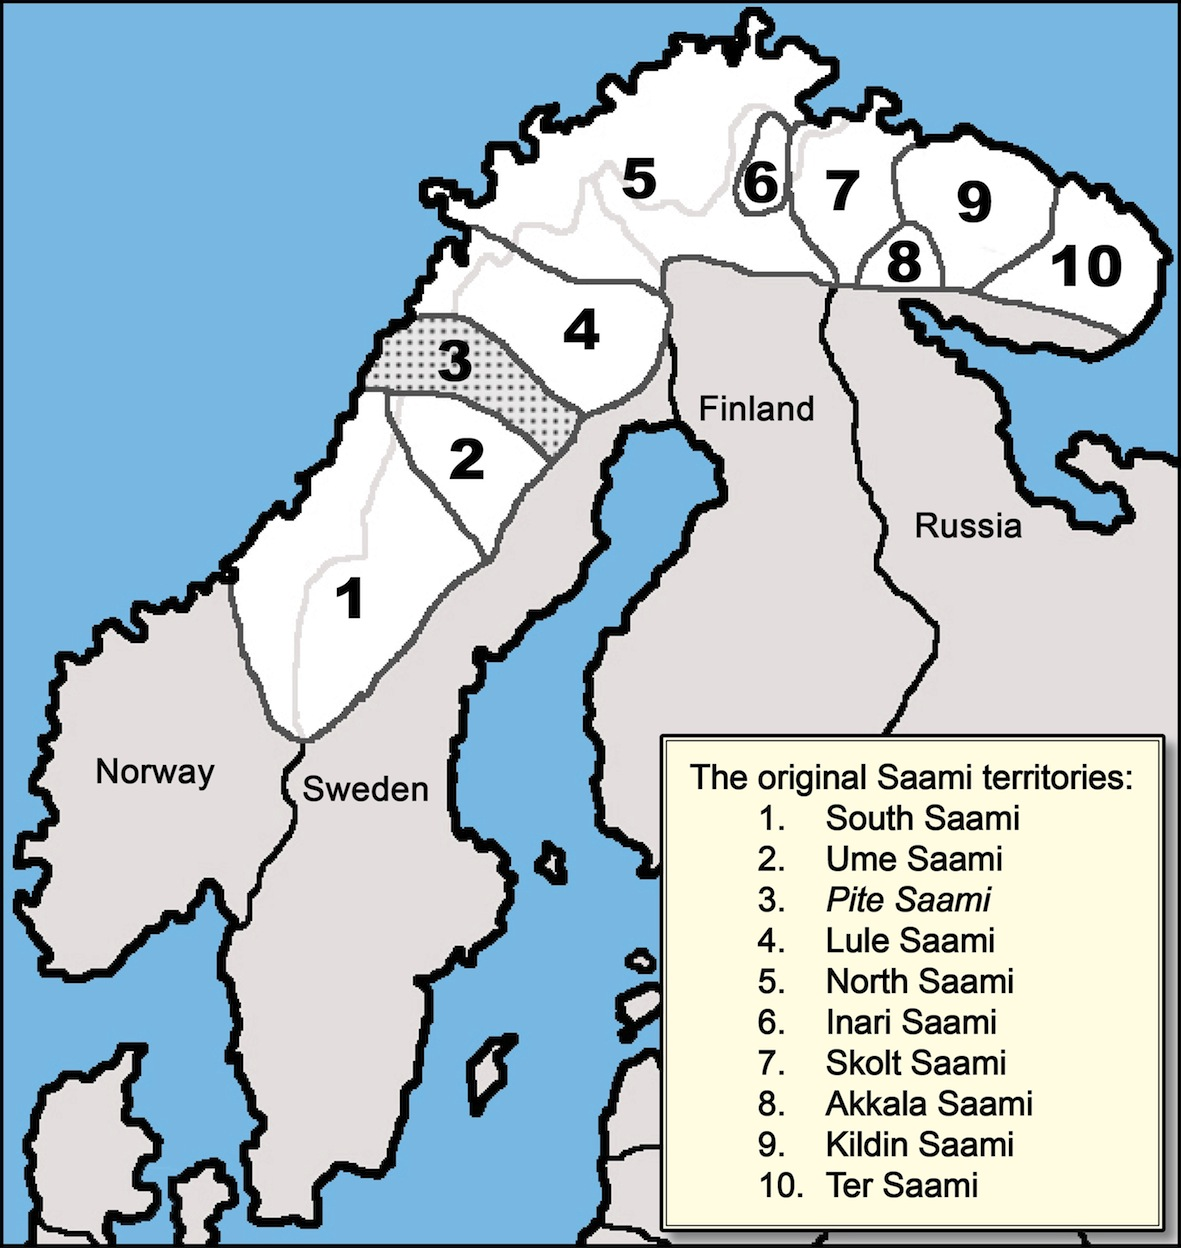
\includegraphics[width=.5\textwidth]{images/SaamiTerritoryMapPiteENsmall.jpg}
\caption[A map of \It{Sápmi}, the territory in which the Saami Languages were traditionally spoken]{A map of Sápmi, the territory in which the Saami Languages were traditionally spoken, with \PS\ shaded in (borrowed from \mbox{\cite[7]{BullEtal2007}}, with permission)}\label{sabme}
\end{figure}

There is no official geographic or political unit defining any \PS\ linguistic or ethnic area, but the individuals (including both speakers and non-speakers) I have met, worked with or heard about who consider themselves to be \PS\ (regardless of language abilities) all come from an area based roughly on the Arjeplog municipality\footnote{Note that Arjeplog \It{municipality} (\It{kommun} in Swedish) refers to the larger administrative district of ca. 15,000 km\superS{2}, while the town of Arjeplog is the main village in the municipality.} 
in Swedish Lapland and bordering areas in Norway. On the Swedish side, this has traditionally been referred to as \It{Pite lappmark} ‘\PS\ territory’. 
For instance, Ruong, himself a native speaker of \PS, claims that the “most genuine form” (Ruong \citeyear[iii]{Ruong1943}; my translation) of the \PS\ language is spoken by members of the Luokta-Mavas \It{sameby},\footnote{A \It{sameby} (Swedish, literally ‘Saami village’; \It{samebyar} in \PL) is a group of reindeer herding families who tend their reindeer together in the same territory.} 
whose summer reindeer grazing lands are located along the headwaters of the Pite River, and by settled Saamis in the same area.\footnote{However, Ruong also included speakers from Semisjaur-Njarg \It{sameby} to the south as sources for his 1945 dissertation on verbal derivation in \PS. It is clear that Ruong is very aware of the existence of the Saami dialect continuum and the difficulty of drawing distinct language borders because he indicates that some areas on the north side of the Pite River drainage speak Lule Saami, while speakers along the Skellefte River drainage are more under the “influence of Southern Saami” (\cite[iii]{Ruong1945}; my translation).} 
Manker’s ethnography of the Saami populations in the Swedish mountains \citep{Manker1947} outlines the three \It{samebyar} Luokta-Mavas, Semisjaur-Njarg and Svaipa as part of \It{Pite lappmark}.\footnote{\citet[473]{Manker1947} includes a map of all Swedish \It{samebyar} as a fold-out, and a map of these three \PS\ villages.} 
\citet[22]{Sammallahti1998} corroborates this, and adds the forest \It{sameby} Ståkke to the list. \citet{Collinder1960} and \citet{Bergsland1962} also help delineate the southern border of \PS\ territory. Collinder writes that the border “goes along the Pite River between the parishes of Jockmock [sic] and Arvidsjaur, and farther west through the parish of Arjeplog” \cite[23]{Collinder1960}, while Bergsland further specifies that Ume Saami is spoken by “the forest Lapps in southern Arjeplog [...] and by the mountain Lapps in Sorsele” \cite[27]{Bergsland1962}. %, thus drawing the southern border of \PS\ at essentially the same place. As for the Norwegian side, in researching his grammar, Lagercrantz (\citeyear{Lagercrantz1926}) worked with two \PS\ speakers whose families originated in the Arjeplog municipality but had resettled to the Beiarn area in Norway. 

As for the Norwegian side, some \PS\ reindeer herding families have had their summer reindeer grazing lands in the Norwegian territory adjacent to the international border \cite[cf.][]{Manker1947}. \citet{Lagercrantz1926} worked with \PS\ speakers whose families originated in the Arjeplog municipality but had resettled to the Beiarn area in Norway. Ethnic \PS\ individuals still live in Norway, and are, for instance, still active in the local \PS\ association, \It{Salten Pitesamisk Forening}. 

As a result, one can say that \PS\ was traditionally spoken in an area spanning both sides of the Norwegian-Swedish border around the municipality of Arjeplog on the Swedish side and across the border into Saltdal and Beiarn municipalities in Norway. %Reindeer herding \PS\ speakers still spend the winter months in the traditional reindeer grazing lands in the lowland forests along the Pite River drainage in Arvidsjaur and Älvsbyn municipalities in Sweden. 
On the Swedish side, the \PS\ area is essentially limited to the Pite River %(\It{Bidumedno}) 
drainage above the waterfall at Storforsen, and the sections of the Skellefte River %(\It{}) 
drainage from the town of Arjeplog and farther upriver. %to the north and south, respectively. 
The map in Figure \vref{piteTerritory} gives a rough idea of the traditional geographic area, which is the light area on the map. It is based on  \citet{Lagercrantz1926}, \citet{Ruong1943}, \citet{Manker1947}, \citet{Bergsland1962} and \citet{Sammallahti1998}, as well as on my own knowledge gained by discussing family histories with \PS\ individuals.

My own research indicates that \PS\ is currently still spoken by a few members of the Luokta-Mavas, Semisjaur-Njarg and Ståkke \It{samebyar}, as well as by settled Saami families from the same areas. Furthermore there are a few individuals from the Arjeplog municipality who have since moved to other areas outside of Arjeplog municipality, %such as along the northern Swedish coast, %(e.g., Luleå, Piteå, Umeå) 
even as far away as southern Sweden. %(e.g., Södertälje, Västerås and Norrköping). 
Ethnic \PS\ individuals from Norway have indicated to me that the last \PS\ speakers on the Norwegian side died several generations ago.%(Knut Sivertsen, p.c.). 

\setlength\fboxsep{0pt}
\setlength\fboxrule{1pt}
\begin{sidewaysfigure}
%\begin{figure}
\centering
\resizebox{\columnwidth}{!}{
\fbox{\includegraphics[width=1\textwidth]{images/motormännens20121115.jpg}}}
\parbox{150mm}{\caption{An approximate map of the territory in which the \PS\ Language was traditionally spoken\label{piteTerritory}}}%NOTE that label is inside caption! otherwise reference in text doesn’t work properly! (cf. http://www.leancrew.com/all-this/2008/09/latex-figure-captions/ )
%\end{figure}
\end{sidewaysfigure}%\end{landscape}

\FloatBarrier
%\clearpage

\subsection{The state of the \PS\ language}\index{language sociology}\index{sociolinguistics}\label{sociolinguistics}
Traditionally, most \PS\ families lived either as semi-nomadic reindeer herders or as sedentary farmers, fishers and hunters. Despite having always been in contact, these two groups lived very different lifestyles, and spoke Saami in relative isolation from one another. While reindeer herding Saami have often been a topic of Saami studies, the settled Saami are neglected or even actively prejudiced against for not being ‘true’ Saami since they do not herd reindeer. The data supporting the present study and gathered as part of \PSDP\ (cf. Section \ref{PSDPcorpus}) originated from both groups.

By the eighteenth century, the Saami peoples had, in general, been converted from animistic polytheism to Christianity, marking the beginning of Saami assimilation to North Germanic culture \citep[cf.][]{Pulkkinen2005}. %\marginpar{how to cite this webpage?!? Cf. Missionary history of Lapland (Pulkkinen, Risto)} %\marginpar{add reference to “the encyclopedia of saami culture (presentation page: http://www.helsinki.fi/~sugl_smi/senc/en/esittely.htm) or other!}. 
Strict policies in the mid-nineteenth century sent \PS\ children to special ‘nomad schools’ where they were not allowed to speak Saami. Attending these schools also kept them away from their families and from regularly participating in \PS\ life, while reinforcing the state’s drive to exclusively promote Swedish culture and social values \citep[cf.][]{ValijarviWilbur2011}. 

Accompanying this shift, traditional realms of \PS\ experience are slowly being left behind in favor of Swedish ones. With the introduction of modern conveniences, most \PS\ individuals have moved to permanent dwellings in populated communities, particularly Arjeplog, thereby leaving behind traditional ways of life. Along with this demographic shift, they are also losing the need to carry out traditional occupations using the \PS\ language. As a result, all \PS\ speakers today speak Swedish fluently, and indeed use Swedish significantly more often in everyday life \citep[cf.][]{ValijarviWilbur2011}.

A gradual reverse in political and social policies in Sweden over the last decades led initially to the acceptance and then to the active promotion of multiculturalism, particularly concerning the Saami people. This has helped to positively change attitudes towards \PS\ identity. However, concerning the \PS\ language and many traditional cultural realms, this change seems inadequate for revitalization. For instance, the Swedish government's minority language law from 2010 only applies the blanket term \It{samiska}, and, in doing so, completely disregards the reality that there are five different Saami languages in Sweden. Even within \It{Sápmi}, \PS\ is threatened by its larger Saami neighbors, in particular by North Saami, which has an active speech community of around 30,000 speakers, regular television, radio, print and internet resources, and first-language instruction in public school \citep[cf.][209-211]{Salminen2007}. The robust status of North Saami in addition to the lack of an officially recognized \PS\ orthography allow local government agencies to conveniently support North Saami alone in fulfilling the language law's requirements; any positive effects on the \PS\ language are essentially negated.

According to my own data collected from \PS\ individuals during fieldwork, there are around 30 speakers left,\footnote{Cf. \citet[221]{Salminen2007}, who claims there are only 10 speakers, while the English abstract in \citet{Lehtiranta1992} erroneously claims that the \PS\ language is “now extinct.”} 
of around 2000 ethnic \PS\ individuals \citep[24]{Krauss1997}. With one exception, all speakers are older than 50. %See Section \ref{geography} for more on the area in which \PS\ is spoken. 
\korr{034}Based on my own observations, all speakers are fluent in the Swedish language, even if many of them did not learn Swedish until they began school. Indeed, Swedish dominates everyday life for most speakers today, particularly for those who do not work in reindeer husbandry, and for those not living in the traditional \PS\ area. Only a few households (less than five) use \PS\ on a regular basis at home or in family situations, and these are still involved in reindeer husbandry. In public realms, the language is rarely used today. For a more detailed description and analysis of the situation the language is currently in, see \citet{ValijarviWilbur2011}.

\FloatBarrier

\section{Linguistic documentation of \PS}\label{lingDoc}
The \PS\ language has been the subject of academic research in the past; cf. \citet{Halasz1896}, \citet{Lagercrantz1926}, \citet{Ruong1943} and \citet{Lehtiranta1992}. %, which are summarized in Section \ref{previousWork} below. 
\korr{077}This extant body of research was consulted in coming to terms with \PS\ linguistic structures in creating the present description. 
However, in fulfilling the goal of describing the \PS\ language as it is spoken in the early 21st century, the \PSDP\ corpus, collected from 2008 through 2013, is the main source of data. With this in mind, I consider this a corpus-based description, as opposed to a literature-based description, which would have attempted to incorporate these previous works to a much greater extent. Indeed, everything not specifically cited as coming from another source is based on my own analysis of the corpus. 
The current description will hopefully be seen as a supplement to previous work on \PS, and, together with previous studies, can facilitate exploring language change as exemplified by a severely endangered language. 

In the following sections, previous studies on \PS\ are summarized in Section \ref{previousWork}. The current corpus and the documentation involved in creating it are described in Section \ref{PSDPcorpus}. Section \ref{usingThis} then provides a short guide to using this description. 

\subsection{Previous studies}\label{previousWork}
In the late 19th century the Hungarian scholar Ignácz Halász studied \PS, and wrote several books in Hungarian on the language. 
\It{Lule- és Pite-lappmarki nyelvmutatvéanyok és szótár}\footnote{‘Linguistic examples and a wordlist from Lule and \PS\ territory’.} \citep{Halasz1885} contains the Gospel of Matthew in Lule Saami, and a combined Lule Saami/\PS\ wordlist with translations in Hungarian and German. 
\It{Népköltési gyüjtemény: a Pite Lappmark Arjepluogi egyházkerületéböl}\footnote{‘Collection of traditional verses from the bishopric of Arjeplog in \PS\ territory’.} \citep{Halasz1893} 
consists of a significant text collection of short \PS\ texts, transcribed in the traditional Finno-Ugric transcription. Each text is translated as a whole into Hungarian. The majority of the texts are traditional narratives, %including some ‘stallo’ (a large, stupid creature common in Saami mythology) stories, 
and a few poems and songs are also transcribed and translated. 
\It{Pite lappmarki szótár és nyelvtan}\footnote{‘Wordlist and grammatical description from \PS\ territory’.} \citep{Halasz1896} 
includes morphological paradigms and a \PS\ wordlist with translations into Hungarian and German. 

\It{Sprachlehre des Westlappischen nach der Mundart von Arjeplog}\footnote{‘A grammar of West Saami based on the Arjeplog dialect’.} \citep{Lagercrantz1926} 
is a grammar in German. It is based on three months of fieldwork during which Lagercrantz consulted three \PS\ individuals who had settled in the Beiarn district in Norway but who were originally from the Arjeplog municipality. The book covers semantically driven descriptions of clause structures, a limited description of morphology, and an extended analysis of the phonological system, based on phonetic acoustic experiments. 

\It{Lappische Verbalableitung dargestellt auf Grundlage des Pitelappischen}\footnote{‘Saami verbal derivation as illustrated by \PS’.} \citep{Ruong1943} is the dissertation of Israel Ruong, who later became professor of Saami languages and culture at Uppsala universitet. Ruong’s native language was \PS; his dissertation, an elaborate categorization of \PS\ verb derivations, is his only study specifically dealing with the \PS\ language. %His dissertation is an elaborate categorization of \PS\ verb derivations. %\marginpar{better description of Ruong1943!}.

\It{Arjeploginsaamen äänne- ja taivutusopin pääpiirteet}\footnote{‘The fundamentals of Arjeplog Saami phonology and inflection’.} \citep{Lehtiranta1992} is a Fin\-nish-language description of \PS\ phonology and inflectional patterns, and is based on recordings, publications and archived materials on \PS\ from 1950 and earlier. Some paradigms can be found at the end of the book, as well as several \PS\ texts with phonetic and orthographic transcriptions, as well as Finnish translations. The phonetic transcriptions are presented in the transcription standard used in Finno-Ugric studies. 

Note that these studies deal with \PS\ as it was spoken before 1950. Finno-Ugristics has traditionally dealt with historic-comparative studies, and has not always been concerned with the synchronic state of Saami languages. Indeed, the distance some scholars keep from the synchronic situation is highlighted by the erroneous claim by Lehtiranta %, as pointed out in a previous footnote, 
that \PS\ is “now extinct” \citep[English abstract]{Lehtiranta1992}. 
Consequently, the present study is the first extensive description in English and for a general linguistic audience on the \PS\ language. % are just now becoming available as a result of the \PSDP\ and the present PhD thesis.%

Since the present study is intended to be a synchronic description of the \PS\ language as used in the early 21\superS{st} century as reflected by the \PSDP\ corpus, the previous studies mentioned above have for the most part played an \korr{056}important but indirect role in its creation. However, these works were referred to in detail particularly when the data from the corpus were not substantial enough to allow relatively certain conclusions to be drawn; data based at least partly on sources other than the documentation corpus are clearly marked as such in this description. Specifically, the sections in \mbox{\citet{Lagercrantz1926}} concerning phrasal and sentence-level syntactic phenomena in Part A ‘\It{Ausdruckslehre}’ (pp. 19-99) were informative, while Part B ‘\It{Formenlehre}’ (pp. 103-141), the paradigms throughout \citet{Halasz1896} as well as the paradigms in the appendix to \citet[150-166]{Lehtiranta1992} were consulted regarding morphology. In writing Chapter \ref{derivMorph} on derivational morphology, Ruong’s thesis  (particularly Chapters 6 through 40, which present his data) provided valuable insights into the variety and complexity of \PS\ derivation from both morphological and semantic perspectives. %; particularly Chapters 6 through 40, which present his data, were considered.

In addition to the academic linguistic studies mentioned above, a number of other texts exist concerning the \PS\ language and its people. \citet{ValijarviWilbur2011} describe the current state of the \PS\ language from the \korr{015} point of view of the sociology of language. \citet{sjaggo2010a} deals with the etymology of a selection of \PS\ place names along the river Piteälven in the Arjeplog municipality. 
A large number of \PS\ \It{vuole}\footnote{This is nominative plural; the nominative singular form is \It{vuolle}.} 
(songs in the Saami singing tradition of \It{yoik}) were recorded in the first half of the 20\superS{th} century. These can be found transcribed in: 
\citet{tiren1942a}, which includes 139 transcriptions of \PS\ melodies and lyrics, with German translations; 
in \citet{grundstroem1958a}, with 93 songs by Jonas Eriksson Steggo in the form of transcribed melodies and lyrics, with translations in Swedish and German; 
as well as in \citet{grundstroem1963a}, with 73 songs by a variety \PS\ individuals in the form of transcribed melodies and lyrics, also with translations in Swedish and German.
%are covered in part in \citet{stoor2007a}. 
\citet{wickman1964} discusses a short \PS\ text from a recording done in 1939 by Israel Ruong; the text is presented in three transcription standards (Finno-Ugric close phonetic standard, the author’s own phonemic transcription, and a modified North Saami orthography) and includes an English translation. 
Lars Rensund’s books (\citeyear{Rensund1982}, \citeyear{Rensund1986}) detail personal recollections by the author, himself a Pite Saami, and are interspersed with sentences and occasionally an entire narrative in \PS. \citet{bylund1956} provides an in-depth study of the colonization of \PS\ territory by Swedish settlers up to the middle of the 19\superS{th} century. 
No educational materials, bible translations or other common texts exist in the \PS\ language. With the exception of the works by Lars Rensund, most \PS\ speakers today are not aware of any of the works mentioned above. 



\subsection{The \PSDP\ corpus}\label{PSDPcorpus}
%\section{The \PSDP\}
The data forming the basis for the present study were collected as a part of the \PSDP. The present grammatical description is also a part of that project, the main goal of which is the linguistic documentation of the \PS\ language. The project has resulted in audio and video recordings documenting current language usage and grammatical structures and includes an archived corpus comprising 29,053 transcribed and translated \PS\ words (as of early March 2014; %January 2013, the \PSDP\ corpus consists of 25,227 %25,227+1815 (added in May 2013)=27042
%transcribed and translated \PS\ words.} %of those recordings and relevant transcriptions and annotations 
cf. the \hyperlink{inventoryRef}{Appendix} for a list of recordings). 
From June 2008 until July 2011, the project was carried out by Joshua Wilbur at the Nordeuropa-Institut at Humboldt-Universität zu Berlin, with support from the \href{http://www.hrelp.org/grants/}{Endangered Languages Documentation Programme} (ELDP; a part of the Hans Rausing Endangered Languages Project, with financial support from the Arcadia foundation and hosted by the School for Oriental and African Studies (SOAS) at the University of London). %Funding consisted of GBP 64,748 over the course of the project to support fieldwork, equipment expenditures, payments for language consultants and to cover a graduate student stipend. 
A continuation of the project is underway in 2013 and 2014 at Albert-Ludwigs-Universität Freiburg thanks to generous continued funding from ELDP. 

Current trends in documentary linguistics were taken into account.\footnote{Cf. \citet{BirdSimons2003}, \citet{Gippert2006}, \citet{Woodbury2011}, \citet{AustinSallabank2011}, \citet{GrenobleFurbee2010} the book series \It{Language Documentation and Description} series, and others.} 
Himmelmann’s proposal that “a language documentation is a lasting multipurpose record of a language” \citep[1]{Himmelmann2006a} is a defining motivation behind the project. Accordingly, the resulting documentation consists of a documentation corpus of a variety of linguistic genres, including \PS\ situations potentially of interest to non-linguistic disciplines and to members of the \PS\ language community themselves, as well as the present grammatical description. Initial results have been archived at five archives at international, national, regional and local levels:
\begin{itemize}
\item{\It{the Endangered Languages Archive} (ELAR) in London, England,}
\item{\It{the Max-Planck Institute for Psycholinguistics} in Nijmegen, the Netherlands,}
\item{\It{Dialekt-, ortnamns och folkminnesarkivet i Umeå}\footnote{‘The Department of Dialectology, Onomastics and Folklore Research in Umeå’.} (DAUM) in Umeå, Sweden,}
\item{\It{Ájtte: Svenskt Fjäll- och Samemuseum}\footnote{‘Ájtte: the Swedish Mountain and Saami Museum’; \It{ájtte} is the Lule Saami word for a traditional Saami storage shed.} in Jokkmokk, Sweden,}
\item{\It{Silvermuseet}\footnote{‘The Silver Museum’.} in Arjeplog, Sweden.}
\end{itemize}
Selecting multiple archiving sites as well as having all data in a digital format and as open-access as possible help ensure the longevity of the data. 

Access to the materials is available via the archives (in some cases, this is possible via the world wide web). %, assuming adherence to access protocol on a file-by-file basis. 
Ideally, an archive should provide interested parties with access to archives materials, while respecting the privacy and the wishes of recording participants as necessary; with this in mind, access rights to the data related to any given session reflect the wishes of speakers involved in a specific session concerning availability to the linguistics and other scientific communities, the \PS\ and greater Saami communities, and other individuals and groups in general. Any commercial use of the materials is strictly prohibited. Specifically regarding the present grammatical description and the documentation corpus as scientifically sound linguistic outcomes, %produced in partial fulfillment of the requirements for the PhD program at Christian-Albrechts-Universität zu Kiel, 
access to the corpus is available via the archive at the Max-Planck Institute for Psycholinguistics in Nijmegen, the Netherlands; see Section \ref{archiveAccess} for more details on accessing the archive. 


\subsubsection{Collection methods}\label{collectionMethods}
Data were collected and recordings were transcribed during a total of 23 months at the field site in and around Arjeplog, Sweden, %Over the course of field work, I was able to develop productive working as well as personal relationships with several native speakers of \PS\ interested at least passingly in documenting their language. 
with the invaluable assistance of a number of \PS\ speakers. They were compensated for their time and effort with a modest consultant honorarium. 

The documentation corpus consists of more than 55 hours of recordings covering a variety of genres; cf. the Appendix for a list of recordings, including an indication of genre and medium. 
As the morphological structure of \PS\ words is quite complex, %(e.g.~17 word forms in a noun paradigm, at least 24 in a verb paradigm), 
it was necessary to rely on elicitation techniques to gather a sufficient number of word forms for a wide variety of lexemes as a basis for morphological analyses. 
As a result, the majority of recordings \korr{035}(approximately 45 hours) consist of elicitation sessions intended to gather specific details concerning the structure of the language. 
These were often conducted using Swedish as a metalanguage, but \PS\ was used whenever efficient and useful, and more frequently in recordings done towards the end of the project. 
A variety of elicitation methods were used; to a large extent, elicitation sessions were conducted as translational interviews (particularly in early recordings to collect initial wordlists) and sentence completion (using both Swedish and \PS\ triggers, mostly to complete morphology paradigms); however, other methods were used as well, such as vocabulary card ordering tasks to test syntactic structures, and tasks using toy blocks to gather data on spatial relations. 
Many non-elicitation linguistic situations were also recorded, covering genres such as conversations, explanations, narrations, performances, as well as songs and readings; in the current documentation corpus, such recordings comprise approximately 17,700 transcribed words. A few written texts were also collected to supplement recordings. 

Each collection of materials\footnote{Note that the archive at the Max-Planck Institute for Psycholinguistics in Nijmegen, the Netherlands, refers to the entire collection of files concerning a single recording as a ‘session’, not a ‘collection’.} 
in the corpus corresponds to a recorded linguistic event. Each collection has a unique name based on the pattern:
\begin{center} pitYYMMDDabc \end{center}
(pit = \PS, YYMMDD = abbreviated date of recording with a two-digit year, abc = further disambiguation as needed).\footnote{Recordings done for the project from 2012 onwards use the ISO 639-3 code \It{sje} as a prefix for session names instead of \It{pit}, and a four-digit year; e.g.: \It{\Bf{sje2012}1014b}.} 
All digital files related to a certain collection are named based on this pattern. 

In almost all cases, the following recording equipment, standards and software were used for documentation. A small number of deviations exist, and are indicated in the metadata for the relevant sessions. 
 
\Bf{Video}: a Panasonic NV-GS500EG-S video camera using miniDV cassettes in short play (SP) mode, using a wide-angle lens attachment and a tripod. In most cases, a RØDE SVM stereo video microphone was mounted on the camera for audio in place of using the built-in microphone.

\Bf{Audio}: an Edirol R-09 digital audio recorder set to record 16-bit WAVE format at 44.1 kHz. A variety of microphones was used, depending on the specific recording situation; these included a RØDE SVM stereo video microphone, a Sennheiser lapel microphone connected to a Sennheiser EW 112-p G2 wireless set and a Sennheiser MKE 300 shotgun microphone. %, and a Sony ECM-MS957 shotgun microphone. %JW: this is Micha’s and Florian’s mic

\Bf{Still images}: a Canon IXUS 80IS digital photo camera was used to take digital photographs to supplement documentation. Images are in JPEG format.

\Bf{Editing/Computing}: video/audio recordings were transferred to a Macintosh MacBook Pro for further editing, as necessary. Video was edited using Final Cut Express and Final Cut Pro software. Audio was archived in the original quality, while video was compressed to MPEG-4 format.

\Bf{Transcribing/annotating}: the multimedia annotation program ELAN\footnote{ELAN is free software developed by the Technical Group of the Max Planck Institute for Psycholinguistics (see \href{http://www.lat-mpi.eu/tools/elan/}{www.lat-mpi.eu/tools/elan/}).} 
was used to transcribe and annotate recordings. Annotation/transcription files are archived in both ELAN format and in plain text format.


Initial transcriptions of recordings were completed with the help of native speaker assistants.\footnote{I am particularly indebted to Elsy Rankvist for her invaluable transcription assistance.} 
Transcriptions \korr{036}in the corpus are written in various versions of the \PS\ orthography under development by the wordlist project \It{Insamling av pitesamiska ord},\footnote{Cf. Section \ref{orthography}.}  %carried out by members of the \PS\ language community. At the time of writing, the project’s orthographic standards have not been fully finalized nor recognized by any official authority. 
but have been standardized according to the principles explained in Section \ref{orthography} when cited in this book. 
All transcribed words are provided with annotations in the form of at least a translation into English or Swedish or as morpheme-by-morpheme glosses. Such glosses can serve as the sole translation of a transcribed word or utterance, particularly concerning transcribed elicitation sessions. Both glosses and free translations into English and/or Swedish may be provided, especially in non-elicited text genres. Relevant notes or commentary may also exist as annotations. 

Metadata were collected in a database using the File Maker Pro program, then exported to XML and plain text formats for archiving. Information collected concerns participants, the recording situation, location, equipment used and a summary of contents, among other things.

Any given collection consists minimally of the following set of digital files: %\footnote{in one case (pit090515), there is no audio recording, but instead a written text, and no additional transcription/annotation files.}
\begin{itemize}
\item{audio recording in WAVE format (16-bit, 44 kHz)}
\item{transcription/annotation file in ELAN and in plain text format}
%\item{transcription/annotation file in plain text format}
\item{metadata concerning the session in XML and plain text formats}
\item{metadata concerning the entire collection in XML and plain text formats}
%\item{}
\end{itemize}
In addition to the above files, collections may also include the following files:
\begin{itemize}
\item{video recording in MPEG-4 format}
\item{digital images in JPEG format}
\item{other supplementary files}
\end{itemize}

The transcription/annotation files are divided into numbered, utterance-based units and include at least a transcription of \PS\ spoken language use. 
A specific utterance can be referred to using the collection/session name and the utterance number. 
The \PS\ original is translated into Swedish and/or English, and provided with linguistic glosses. Other comments are included as well, whenever deemed relevant or useful. 
Finally, in cases with code-switching, the language being used in a certain utterance, or part thereof, is indicated. Tiers in all ELAN files are organized hierarchically based on the template %illustrated %removed to keep extra line from being added in final formatting!
in Figure \vref{ELANhierarchy} for each speaking participant in a recording, plus a ‘notes’ tier for general comments. %\marginpar{or should this be considered a Table?}.
\newcommand{\Descr}{30mm}%sets x-axis length for tier descriptions
\begin{figure}\centering
%\resizebox{\columnwidth}{!}{%
\begin{tikzpicture}
\draw [blue,ultra thick] (-3mm,0mm)--(6mm,0mm) node[anchor=west,black]{ref};
\draw [blue,ultra thick] (5mm,0mm)--(5mm,-30mm)--(11mm,-30mm) node[anchor=west,black]{lang};
\draw [blue,ultra thick] (5mm,-25mm)--(11mm,-25mm) node[anchor=west,black]{nt};
\draw [blue,ultra thick] (5mm,-5mm)--(11mm,-5mm) node[anchor=west,black]{text};
\draw [blue,ultra thick] (10mm,-10mm)--(16mm,-10mm) node[anchor=west,black]{ftrLing};
\draw [blue,ultra thick] (10mm,-15mm)--(16mm,-15mm) node[anchor=west,black]{ftrE};
\draw [blue,ultra thick] (10mm,-5mm)--(10mm,-20mm)--(16mm,-20mm) node[anchor=west,black]{ftrS};
\draw [blue,ultra thick] (-3mm,-35mm)--(6mm,-35mm) node[anchor=west,black]{notes};
\draw [font=\itshape,red,ultra thick,densely dashed] (-3mm,-35mm)--(-3mm,1.8mm) node[anchor=south]{root};%root bar
\draw (\Descr,0mm) node[font=\footnotesize,anchor=west]{Assigns each utterance a number and time alignment};
\draw (\Descr,-5mm) node[font=\footnotesize,anchor=west]{Transcription of utterance in \PS\ orthography};
\draw (\Descr,-10mm) node[font=\footnotesize,anchor=west]{Linguistic glossing};
\draw (\Descr,-15mm) node[font=\footnotesize,anchor=west]{Free translation in English};
\draw (\Descr,-20mm) node[font=\footnotesize,anchor=west]{Free translation in Swedish};
\draw (\Descr,-25mm) node[font=\footnotesize,anchor=west]{Notes on the utterance};
\draw (\Descr,-30mm) node[font=\footnotesize,anchor=west]{Langauge used};
\draw (\Descr,-35mm) node[font=\footnotesize,anchor=west]{General comments};
\draw [black] (-8mm,7mm)--(103mm,7mm);%header line
\draw [black] (-8mm,-38mm)--(103mm,-38mm);%footer line
\draw (9mm,9.2mm) node[font=\itshape\footnotesize,anchor=west]{tier name};
\draw (-8mm,9mm) node[font=\itshape\footnotesize,anchor=west]{hierarchy};
\draw (\Descr,8.7mm) node[font=\itshape\footnotesize,anchor=west]{purpose};
\end{tikzpicture}%}
\caption{ELAN tier hierarchy used in the documentation corpus}\label{ELANhierarchy}
\end{figure}

 A list of all recordings in the corpus can be found in the Appendix on page \pageref{inventory}, including brief descriptions of content and an indication of the number of \PS\ words transcribed and translated per recording. 




\subsection{Using this description}\label{usingThis}  
This description of the grammar and the accompanying documentation corpus are intended to outline the structural features of the \PS\ language and provide an empirical foundation for such claims. In addition, the documentation should give interested individuals (linguists, Saami individuals, etc.) the opportunity to explore other aspects of the language as well. Finally, it should also secure a record of the language as spoken by those \PS\ individuals who likely comprise the last generations of speakers for future generations of ethnic \PS\ individuals. 

%\Red{UPDATE THIS: } 
The following sections are meant to assist in utilizing both the grammatical description and the accompanying documentation corpus. 
The first section (\ref{accountabilityEtc}) deals with accountability and verifiability, while the second section (\ref{archiveAccess}) provides brief instructions on how to access data from the corpus. 
Section \ref{orthography} covers orthographic considerations and includes a list of phonemes and the graphemes used to represent these.  
Section \ref{examplesExample} illustrates how examples from the corpus are presented. %, and Section \ref{organizationalPrinciples} briefly discusses the organizing principles used to structure the grammatical description. 
Note that a list of abbreviations and a list of symbols used in the present work are provided on pages \pageref{abbreviations} and \pageref{symbolList}, respectively. 


\subsubsection{Accountability and verifiability}\label{accountabilityEtc}
Data in the present study are cited with a reference to the collection name followed by the specific utterance number or timecode within a recording. For instance, the reference \It{pit080924.366} refers to utterance number \It{366} on recording \It{pit080924}. %(made on 24\superS{th} September 2008). 
This should allow the reader to easily find the evidence cited and make his/her own judgement about the conclusions made. References to specific recordings marked with ‘(\It{elic.})’ indicate that the chosen utterance was attained during an elicitation session. 

In order to verify, scrutinize or otherwise review the actual primary data on which the present study is based, the data can be accessed via one of the archives listed in Section \ref{PSDPcorpus}. Specific instructions are provided in the following section. 


\subsubsection{Accessing archived materials}\label{archiveAccess}
The archivists at the IMDI archive located at the Max Planck Institute for Psycholinguistics in Nijmegen, the Netherlands, have kindly agreed to host the \PSDP\ spoken language corpus. For those interested in accessing the data in connection with the present grammatical description, I recommend using this archive. \PS\ materials are available via the on-line IMDI-browser at: 
\begin{center}\href{http://corpus1.mpi.nl/ds/imdi_browser/}{corpus1.mpi.nl/ds/imdi\_browser/}
\end{center}
under the hierarchical node:
\begin{center}\href{http://corpus1.mpi.nl/ds/imdi_browser/?openpath=MPI1565580\%23}{ Endangered Languages/Donated Corpora/Pan-Saami Language Archive/Pite}
\end{center}
%The core purpose of any archive is to keep its ‘artefacts’ preserved, and accessible to future generations. Hopefully…
%Metadata can be accessed by anyone; in order to access the actual media files or transcription and annotation files, a user account is required and can be set up via the same website. Please contact the author by email at \href{mailto:joshwilbur@gmx.net}{\fontspec{Courier}\mbox{joshwilbur@gmx.net}} for more information. 


\subsubsection{Explaining examples}\label{examplesExample}\hypertarget{explExs}
Examples from the corpus are numbered consecutively for easy reference, and consist of several lines of text. The spoken text is presented in the initial line in the orthographic standard in italics, followed by interpretive information in the form of a morpheme-for-morpheme breakdown in the second line and English glosses in the third line. Finally, the last line contains a free translation in English and a reference to the source recording in the corpus; this reference includes either the number of the specific utterance or its initial time code. Examples are formatted as shown in Figure \vref{exampleExplanation}.
\begin{figure}
\hspace{-7pt}\begin{tabular}{p{.06\columnwidth} p{.90\columnwidth}}
(no.)&\It{\PS\ original text}\\
	& \PS\ text with morpheme boundarie-s\\
	& Morpheme-for-morpheme glossing \\%\Sc{with grammatical categories in small caps}\\
	& ‘free English translation’\hbox{}\hfill{\small\textnormal{[source]}}\\ %\hspace*{200pt} \small\textnormal{[source]}\normalsize
\end{tabular}
\caption{Formatting pattern used in examples of utterances}\label{exampleExplanation}
\end{figure}

In Chapter \ref{ProsodicStructure} on prosody and Chapter \ref{csANDvs} on segmental phonology, many examples of individual words are provided to illustrate phonological aspects of \PS. In most cases, the phonological representation and phonetic realization (both using IPA standards) and the orthographic representation (based on the current working version) are included, as well as a gloss and a reference to the source recording, as summarized in Figure \vref{exampleExplanationWords}. In such the examples, the phonemic representation also indicates any linear morpheme boundaries. 
\begin{figure}
(no.)\hspace{1em}
\begin{tabular}{p{30mm} l}
/phonemic/ 		& \It{orthography}	\\%\MR{2}{*}{\hfill\small[source]} \\
\MC{1}{l}{[phonetic]}	& ‘gloss’			\\
\end{tabular}\hfill\small[source]
\caption{Formatting pattern used in examples for individual words}\label{exampleExplanationWords}
\end{figure}
%\noindent 
%\label{wordlistReference}
The source recording for these words indicates the recording name and utterance number or time code in most cases. However, when only a four-digit number is present (e.g.: {\small[0457]}), this indicates that the original recording is not from the documentation corpus, but from the Wordlist Project (cf. Section \ref{orthography}). The number refers to the record number of the word in the Wordlist Project’s lexical database, and the accompanying recording of that specific wordlist item, as collected by the members of the Wordlist Project. Currently, the recordings of the entries in the wordlist have not been archived, but will likely be archived in the near future once the permission of the members of the Wordlist Project has been secured. Some examples in Chapter \ref{derivMorph} on derivational morphology are also from this lexical database, and are marked in the same way. 


\subsubsection{Orthographic considerations}\label{orthography}
At the time of writing, \PS\ does not have an officially recognized orthography. In the past, adapted versions of the Swedish orthographic standards\footnote{Cf. Lars Rensund’s books (\cite{Rensund1982}, \citeyear{Rensund1986}).} 
and Lule Saami orthographies\footnote{E.g., at literacy courses for \PS\ individuals held in Arjeplog occasionally during the last decade and sponsored by the Swedish Saami Parliament.} 
have been used to write \PS\ for a non-technical, non-linguistic audience. However, from 2008 through 2011, \It{Arjeplogs sameförening} (the local Saami association in Arjeplog) received funding to complete a lexicographic project called \It{Insamling av pitesamiska ord},\footnote{This translates roughly as “collecting \PS\ words”. A working version of the resulting lexical database is currently available online at: \href{http://gtweb.uit.no/webdict/index_sje-swe.html}{http://gtweb.uit.no/webdict/index\_sje-swe.html}.} 
\citep[cf.][]{insamlingPS2011} 
and hereinafter referred to simply as ‘the \WLP’. 
One of the outcomes of the \WLP\ was a working orthography for \PS. 
%As part of the \PS\ Documentation Project, I worked closely with the members of the \WLP\ as an unofficial linguistics consultant and 
I have attempted to adopt this working orthographic standard in writing \PS\ data in this description and the transcriptions provided in the accompanying documentation. This orthography uses the Swedish alphabet and many Swedish sound-to-grapheme correspondences, but also resembles to some extent Lule Saami orthographic systems, particularly the most recent one as found in \citet{KorhonenO2005}. To help understand the orthography, the correlations between sounds and graphemes are discussed here and listed in Table \ref{orthTableC} starting on page \pageref{orthTableCbegin} for consonants, and in Table \vref{orthTableV} for vowels. %\marginpar{this table was just copied in - it needs to be re-worked, checked!!!}
\korr{057}Chapter \ref{csANDvs} describes the segmental phonology represented by these graphemes in detail. 
An orthography proposal for the \PS\ language, including a more thorough description of these rules, is currently being put together by the members of the \WLP, the Arjeplog municipality, and the \PSDP, and is scheduled to be published in late 2014, along with a printed version of the \WLP’s word list.

It is important to note that the standards used in this book are based on a \It{working} orthography, i.e., it is still subject to inconsistencies and potentially to further refinement. Moreover, the following description and the implementation of the orthography is based on my interpretation of the recurring patterns used by the \WLP\ as determined in developing the orthography proposal mentioned above. While I generally use the spellings found in the \WLP’s wordlist, some deviations may be found in this description and the accompanying transcriptions; these can be due to a variety of factors such as changes to the word list as it was developed, deviating analyses on my own behalf, or simple inconsistencies in spelling (a natural occurrence in the development of an orthography) in the source. However, I alone am ultimately responsible for the orthographic choices in the present work. 

%%new command for this section on orthographic examples; syntax: #1=orthography, #2=phonology, #3=gloss
\newcommand\SpellEx[3]{\Tn{\begin{tabular}{p{70pt} p{70pt} l}/#2/&\It{#1}& ‘#3’ \\\end{tabular}}}

The unaspirated singleton plosive phonemes are normally represented by the digraphs <b>, <d> and <g>, except as a single word-final consonant, in which case <p>, <t> and <k> are used; this is illustrated by the alveolar plosive phoneme /t/ in \REF{spellExPlos1a} through \REF{spellExPlos1c}. 
\ea\label{spellExPlos1a}
\SpellEx{\Bf{d}állve}{\Bf{t}aːlːve}{winter}
\z
\ea\label{spellExPlos1b}
\SpellEx{bå\Bf{d}av}{pɔ\Bf{t}av}{come (\Sc{1sg.prs})}
\z
\ea\label{spellExPlos1c}
\SpellEx{båhte\Bf{t}}{pɔʰte\Bf{t}}{come (\Sc{inf})}
\z

\korr{016}The affricate phonemes are represented by the digraphs <ts> and <tj>; this is illustrated in \REF{spellEx0a} and \REF{spellEx0b}. 
\ea\label{spellEx0a}
\SpellEx{\Bf{ts}igget}{\Bf{ʦ}igːet}{set up}
\z
\ea\label{spellEx0b}
\SpellEx{alma\Bf{tj}}{alma\Bf{ʧ}}{person}
\z

In general, geminate consonants are written by doubling the relevant letter, as illustrated in \REF{spellEx1} through \REF{spellEx3}. 
\ea\label{spellEx1}
\SpellEx{gå\Bf{dd}et}{kɔ\Bf{tː}et}{kill}
\z
\ea\label{spellEx2}
\SpellEx{ká\Bf{ff}a}{kaː\Bf{fː}a}{coffee}
\z
\ea\label{spellEx3}
\SpellEx{ma\Bf{ŋŋ}el}{ma\Bf{ŋː}el}{after}
\z
However, geminate segments represented by\korr{017} digraphs, such as <sj> for /ʃ/ or <tj> for /ʧ/ %\marginpar{technical term for ‘a combination of letters’?} 
are written by doubling the initial letter, as in \REF{spellEx4} through \REF{spellEx5b}.
\ea\label{spellEx4}
\SpellEx{bå\Bf{ssj}o}{pɔ\Bf{ʃː}o}{kitchen}
\z
\ea\label{spellEx5}
\SpellEx{ma\Bf{nnj}e}{ma\Bf{ɲː}e}{daughter-in-law}
\z
\ea\label{spellEx5b}
\SpellEx{gå\Bf{ttj}åt}{kɔ\Bf{ʧː}ɔt}{urinate}
%\SpellEx{i\Bf{ttj}i-j}{i\Bf{ʧː}ij}{\Sc{neg}-\Sc{3sg.pst}}
\z

Preaspiration is represented by <h> when the preaspirated segment is the initial segment in the consonant center, as in \REF{spellEx6} and \REF{spellEx7}. 
%For preaspirated geminates, the aspiration is represented by <h>, while the long consonant is indicated by doubling the relevant letter, as in \REF{spellEx6} through \REF{spellEx7}. 
\ea\label{spellEx6}
\SpellEx{bå\Bf{ht}et}{pɔ\Bf{ʰt}et}{come}
%\ea\label{spellEx6b}
%\SpellEx{mä\Bf{htts}e}{mɛ\Bf{ʰʦː}e}{forest}
%%\SpellEx{ä\Bf{htts}et}{ɛ\Bf{ʰʦʦ}et}{love}
\z
\ea\label{spellEx7}
\SpellEx{á\Bf{httj}e}{aː\Bf{ʰʧː}e}{father}
\z
If a preaspirated segment is preceded by a sonorant consonant segment, then the preaspiration itself is not marked by a grapheme of its own, as in \REF{spellEx8} through \REF{spellEx10}.
\ea\label{spellEx8}
\SpellEx{mu\Bf{rrk}o}{mu\Bf{rːʰk}o}{fog}
\z
\ea\label{spellEx9}
\SpellEx{gu\Bf{mmp}e}{ku\Bf{mːʰp}e}{wolf}
\z
\ea\label{spellEx10}
\SpellEx{vua\Bf{nnts}a}{vu͡a\Bf{nːʰʦ}a}{hen}
\z
For plosives, the preaspiration is evident nonetheless because the corresponding plain segments are spelled differently, using <b, d, g>. However, the current working version of the orthography does not provide a way to distinguish between preaspirated affricates preceded by a sonorant segment, e.g.~\REF{spellEx10}, and plain affricates preceded by a sonorant segment. 
%\begin{exe}
%\ea\label{spellEx11}
%\SpellEx{vua\Bf{nnts}a}{vu͡a\Bf{nːʰʦ}a}{hen}
%\z

In spoken \PS, when the copula and auxiliary verb \It{lä} is preceded by a word ending in an open syllable, it is often encliticized as \It{l} on that preceding word. To reflect this in the orthography, \It{lä} is then written as \It{’l} immediately following the preceding word, as in \REF{IScliticEx1} and \REF{IScliticEx2}. 
\newcommand{\cliticExs}[3]{\Tn{\begin{tabular}{p{30mm} c p{30mm} p{35mm}}\It{#1}&\ARROW &\It{#2} & ‘#3’\\\end{tabular}}}%specifically for the next two examples
\ea\label{IScliticEx1}
\cliticExs{gunne \Bf{lä} dån}{gunne\Bf{’l} dån}{where are you?}
%gunne \Bf{lä} dån \ARROW\ gunne\Bf{’l} dån \hspace{20pt} ‘where are you?’
\z
\ea\label{IScliticEx2}
\cliticExs{dállke \Bf{lä} bivval}{dállke\Bf{’l} bivval}{the weather is warm}
%dállke \Bf{lä} bivval \ARROW\ dállke\Bf{’l} bivval \hspace{20pt} ‘the weather is warm’
\z

%for orthography tables:
\newcommand\Grapheme[1]{\Bf{#1}}
\newcommand\IPA[1]{#1}

%\begin{table}\centering
\label{orthTableCbegin}
\begin{longtable}[c]{| c  c | l |}
\caption{Consonant phonemes and their corresponding graphemes/digraphs in the working-version of the \PS\ orthography\label{orthTableC}}\\%longtable-caption a bit special: needs \label{} inside caption, needs \\ at end of line, comes after \begin{longtable}{cclr}... 
\hline
\It{phoneme}	&\It{letter or}	&		\\
\It{(IPA)}		&\It{letters}	&\It{context}	\\\hline%& example \\\hline
\endfirsthead
\caption[]{Consonant phonemes and their corresponding graphemes/digraphs in the working-version of the \PS\ orthography}\\%longtable-caption a bit special: needs \label{} inside caption, needs \\ at end of line, comes after \begin{longtable}{cclr}... !!!But this then gets an entry in the List of Tables for each page the longtable-header is on, unless \caption[] used here, and \endfirsthead above
\hline
\It{phoneme}	&\It{letter or}	&		\\
\It{(IPA)}		&\It{letters}	&\It{context}	\\\hline%& example \\\hline
\endhead
\IPA{p}	&\Grapheme{b}		& default grapheme \\*
		&\Grapheme{p}		& word-finally; first C in a C-cluster \\\hline
\IPA{ʰp}	&\Grapheme{hp}	& default digraph	\\*
		&\Grapheme{p}		& after sonorant C in C-center	\\\hline%& \It{gummpe} ‘wolf’ \\\hline
\IPA{pː}	&\Grapheme{bb}	& default digraph \\*%\hline
		&\Grapheme{pp}	& first segment in a C-cluster \\\hline %; (inconsistently intervocalically)	\\\hline
\IPA{ʰpː}	&\Grapheme{hpp}	& default digraph	\\\hline
\IPA{t}	&\Grapheme{d}		& default grapheme \\*
		&\Grapheme{t}		& word-finally; first C in a C-cluster\\\hline
\IPA{ʰt}	&\Grapheme{ht}	& default digraph	\\*
		&\Grapheme{t}		& after sonorant C in C-center \\\hline%& \It{virrtit} ‘must’ \\\hline
\IPA{tː}	&\Grapheme{dd}	& default digraph \\*%\hline
		&\Grapheme{tt}		& first segment in a C-cluster \\\hline %; (inconsistently intervocalically)	\\\hline
\IPA{ʰtː}	&\Grapheme{htt}	& default digraph	\\\hline
\IPA{k}	&\Grapheme{g}		& default grapheme \\*
		&\Grapheme{k}		& word-finally; first C in a C-cluster\\\hline
\IPA{ʰk}	&\Grapheme{hk}	& default digraph	\\*
		&\Grapheme{k}		& after sonorant C in C-center \\\hline%& \It{fuällke} ‘family’ \\\hline
\IPA{kː}	&\Grapheme{gg}	& default digraph \\*%\hline
		&\Grapheme{kk}	& first segment in a C-cluster \\\hline %; (inconsistently intervocalically)	\\\hline
\IPA{ʰkː}	&\Grapheme{hkk}	& default digraph	\\\hline

\IPA{ʦ}	&\Grapheme{ts}	& default digraph	\\\hline
%		&\Grapheme{dts}	& /ʦː/ (geminate) \\\hline
\IPA{ʰʦ}	&\Grapheme{hts}	& default digraph	\\*
%		&\Grapheme{htts}	& sequence of two /ʰʦ/ (geminate)	\\*%\hline%& \It{mähttse} ‘forest’ \\\hline
		&\Grapheme{ts}	& after sonorant C in C-center \\\hline%& \It{vuanntsa} ‘hen’ \\*%\hline
\IPA{ʦː}	&\Grapheme{dts}	& default digraph \\\hline
%		&\Grapheme{tts}	& before unvoiced or preaspirated C \\\hline %; (inconsistently intervocalically)	\\\hline
\IPA{ʰʦː}	&\Grapheme{htts}	& default digraph	\\\hline

\IPA{ʧ}	&\Grapheme{tj}		& default digraph	\\\hline
%		&\Grapheme{dtj}	& /ʃː/ (geminate) \\\hline
\IPA{ʰʧ}	&\Grapheme{htj}	& default digraph	\\*
%		&\Grapheme{httj}	& sequence of two /ʰʧ/ (geminate)	\\*%\hline%& \It{mähttse} ‘forest’ \\\hline
		&\Grapheme{tj}		& after sonorant C in C-center \\\hline%& \It{vuanntsa} ‘hen’ \\*%\hline
\IPA{ʧː}	&\Grapheme{dtj}	& default digraph \\\hline
%		&\Grapheme{ttj}	& second member C \\\hline %; (inconsistently intervocalically)	\\\hline
\IPA{ʰʧː}	&\Grapheme{httj}	& default digraph	\\\hline

\IPA{f}	&\Grapheme{f}		& default grapheme	\\\hline
\IPA{f:}	&\Grapheme{ff}		& default digraph	\\\hline
\IPA{v}	&\Grapheme{v}		& default grapheme	\\\hline
\IPA{vː}	&\Grapheme{vv}	& default digraph	\\\hline
\IPA{s}	&\Grapheme{s}		& default grapheme	\\\hline
\IPA{sː}	&\Grapheme{ss}	& default digraph	\\\hline
\IPA{ʃ}	&\Grapheme{sj}	& default digraph	\\\hline
\IPA{ʃː}	&\Grapheme{ssj}	& default digraph	\\\hline
%		&\Grapheme{ssj}	& sequence of two /ʃ/ (geminate)	\\\hline
\IPA{h}	&\Grapheme{h}		& default grapheme	\\\hline
\IPA{m}	&\Grapheme{m}	& default grapheme	\\\hline
\IPA{mː}	&\Grapheme{mm}	& default digraph	\\\hline
\IPA{n}	&\Grapheme{n}		& default grapheme	\\\hline
\IPA{nː}	&\Grapheme{nn}	& default digraph	\\\hline
\IPA{ɲ}	&\Grapheme{nj}	& default grapheme	\\\hline
\IPA{ɲː}	&\Grapheme{nnj}	& default digraph	\\\hline
%		&\Grapheme{nnj}	& sequence of two /ɲ/ (geminate)	\\\hline
\IPA{ŋ}	&\Grapheme{ŋ}		& default grapheme	\\\hline
\IPA{ŋː}	&\Grapheme{ŋŋ}	& default digraph	\\\hline
\IPA{r}	&\Grapheme{r}		& default grapheme	\\\hline
\IPA{rː}	&\Grapheme{rr}		& default digraph	\\\hline
\IPA{l}	&\Grapheme{l}		& default grapheme	\\\hline
\IPA{lː}	&\Grapheme{ll}		& default digraph	\\\hline
\IPA{j}	&\Grapheme{j}		& default grapheme	\\\hline
\IPA{jː}	&\Grapheme{jj}		& default digraph	\\\hline
%\end{tabular}
\end{longtable}
\label{orthTableCend}


\begin{table}\centering
\caption{Vowel phonemes and their corresponding graphemes/digraphs in the working-version of the \PS\ orthography}\label{orthTableV}
\begin{tabular}[t]{| c  c | l |}\hline
%\MC{3}{|c|}{\BfIt{vowels}}\\\hline
\It{phoneme}	&\It{letter or}	&		\\
\It{(IPA)}		&\It{letters}	&\It{context}	\\\hline%& example \\\hline
\IPA{aː}	&\Grapheme{á}		& default grapheme	\\\hline
\IPA{a}	&\Grapheme{a}		& default grapheme	\\\hline
\IPA{ɛ}	&\Grapheme{ä}		& default grapheme	\\\hline
\IPA{e}	&\Grapheme{e}		& default grapheme	\\*
		&\Grapheme{ie}	& in V1	\\\hline%&\It{diehtet} ‘know’  \\\hline
\IPA{i}	&\Grapheme{i}		& default grapheme	\\\hline
\IPA{u}	&\Grapheme{u}		& default grapheme	\\\hline
\IPA{o}	&\Grapheme{o}		& default grapheme	\\*
		&\Grapheme{uo}	& in V1	\\\hline%&\It{guolle} ‘fish’  \\\hline
\IPA{ɔ}	&\Grapheme{å}		& default grapheme	\\\hline
\IPA{u͡a}	&\Grapheme{ua}	& default digraph	\\*
		&\Grapheme{uä}	& allophone (umlaut) \\\hline%& \It{buäjjde} ‘fat’ \\\hline
%		&\Grapheme{uä}	& allophone (umlaut)\footnotemark \\\hline%& \It{buäjjde} ‘fat’ \\\hline
\end{tabular}
\end{table}
%\footnotetext{Cf. Section \ref{Vua}.}

\FloatBarrier

\section{Typological profile}\label{typologicalProfile}
\PS\ is a Western Saami language in the Saamic branch of the Uralic language family. It is currently spoken by around thirty speakers in and around the Arjeplog municipality in Swedish Lapland. (Cf. Section \ref{PSbackground} for more details on the current state of the language.) 

With the exception of a limited number of grammatical items, \PS\ words consist minimally of one trochaic foot. All non-final odd syllables are stressed, with the initial syllable being most prominent. (Cf. Chapter \ref{ProsodicStructure}.) 

There are 43 native consonant phonemes and 9 native vowel phonemes. With the exception of the glottal fricative /h/, there is a length distinction for all consonants (singleton and geminate pairs). There are both voiceless and preaspirated plosive and affricate phonemes. Geminates and preaspirated segments are restricted to foot-medial position. Vowel length is only distinctive in open front position (/a/ and /aː/). (Cf. Chapter \ref{csANDvs}.) 


Linear morphology in \PS\ is exclusively suffixing. However, grammatical categories are often expressed non-linearly as well. This can take the form of foot-internal consonant alternations, umlaut vowel of the initial foot, and regressive vowel harmony between both vowels of a foot. 

Nouns inflect for nine cases and number. Verbs inflect for person, number, tense and mood. Adjectives come in sets of attributive and predicative forms that are not regularly derivable from one another; attributive adjectives do not inflect, while predicative adjectives inflect for number. Number distinctions are limited to singular and plural for nouns, non-personal pronouns and predicative adjectives, but also exhibit a dual form in pronouns and in verb agreement morphology. (Cf. Chapter \ref{morphology} for a brief introduction to \PS\ morphology; details on inflectional morphology can be found throughout Chapters \ref{nouns} through \ref{otherWordClasses}.) 

There are seven word classes (verbs, nominals, adjectivals, adverbs, postpositions, conjunctions and interjections); these can be distinguished by syntactic criteria as well as their behavior concerning inflectional morphology. Nouns, verbs, adjectives and adverbs can be derived using linear and/or non-linear morphological processes. (Cf. Chapter \ref{introWordForms} for a more detailed overview of the various word forms; Chapter \ref{nouns} on nouns; Chapter \ref{pronouns} on pronouns; Chapter \ref{adjectivesIntro} on adjectivals; Chapter \ref{verbs} on verbs; Chapter \ref{otherWordClasses} on the other word classes; Chapter \ref{derivMorph} provides some examples for derivational morphology.) 

Nominal phrases, adjectival phrases, adverbial phrases and postpositional phra\-ses and the verbal complex constitute the main components of \PS\ clauses, and are covered in Chapter \ref{phraseTypesCh}. 

\PS\ has nominative/accusative argument alignment. 
Basic clauses consist minimally of a single finite verb form and potentially a further non-finite verb form, %, depending on whether the finite verb form is a modal verb, the auxiliary verb or the negation verb, 
as well as any arguments, complements, adjuncts and particles. Copular clauses require the fully inflected copular verb. Negation is expressed by the fully inflected verb of negation in combination with a special non-finite form of the negated lexical verb. Polar interrogatives can be identified by a question marker, but this is exceptionally rare in current \PS\ usage. Clause-level possession can be expressed using a transitive verb with the possessor as the subject and the possessum as the object, or using a copula phrase with the possessum as the subject and the possessor in an oblique case. Relativization uses a relative pronoun embedded in a relative clause with a fully inflected finite verb; the relative pronoun is not restricted in the syntactic role it has in the relative clause. Constituent order is not determined syntactically, but by information structure. (Chapters \ref{overviewSyntax} through \ref{complexClauses} deal with clause-level syntax.) 

The \PS\ language exhibits a number of features which are potentially remarkable from a general typological point of view, even if most of these features are not particularly unusual among the Saami languages. A selection of such features and the sections they are dealt with in are listed in Table \vref{freakyShit}. 

\newcommand{\Feat}[2]{\HANG #1&\ref{#2}\\\hline}%for the following table only
\newcommand{\FeatTwo}[3]{\HANG #1&\ref{#2}, \ref{#3}\\\hline}%for the following table only, when two refs are needed
\begin{table}\centering
\caption{A selection of potentially interesting features in \PS\ from a typological perspective}\label{freakyShit}
\resizebox{1\linewidth}{!} {
\begin{tabular}{|p{.83\columnwidth}|p{40pt}|}\hline
\It{Feature}	&\It{Section}	\\\dline
\Feat{utterance-final voicelessness}{utteranceFinalDevoicing}
\Feat{preaspirated phonemes}{preaspiration}
\Feat{phonemic length distinction for all consonants}{geminateCs}
\Feat{morphological categories commonly expressed by ablaut}{morphophonology}
%\Feat{nouns inflect for possession}{possSuffixes}%gar nicht so außergewöhnlich
\FeatTwo{three-way number distinction in personal pronouns and verb agreement}{personalPronouns}{personNumberVerbs}
\Feat{irregular distinction between attributive and predicative adjectives}{notePredNounsAdjs}
\Feat{suppletion in the lexeme for ‘small’}{smallADJs}
\Feat{potential mood in verbal inflection}{POTmood}
\Feat{negation expressed by a finite negation verb}{negationVerb}
\Feat{predicative possession expressed by either locative or ‘have’-verb}{copulaClauses}
\Feat{no regular distinction between polar interrogatives and declaratives}{polarQs}
\end{tabular}}
\end{table}

















%%%%%%% THIS IS NOT USED FOR THE ENTIRE COMPILATION, but only for individual chapters!!!!

\clearpage
\addcontentsline{toc}{chapter}{Bibliography}\label{Bibliography}
\bibliography{PiteGrammarBibSDL}%for bibtex
%\printbibliography%[title=Works Cited]%%for biber!






%%%NAME INDEX doesn’t work!?!? why???
\cleardoublepage\phantomsection%this allows hyperlink in ToC to work
\addcontentsline{toc}{chapter}{Name index}
\ohead{Name index}
\printindex[aut]

\cleardoublepage\phantomsection%this allows hyperlink in ToC to work
\addcontentsline{toc}{chapter}{Language index}
\ohead{Language index}
\printindex[lan]

\cleardoublepage\phantomsection%this allows hyperlink in ToC to work
\addcontentsline{toc}{chapter}{Subject index}
\ohead{Subject index}
\printindex


\end{document}%
%\documentclass[ number=5
			   ,series=sidl
			   ,isbn=xxx-x-xxxxxx-xx-x
			   ,url=http://langsci-press.org/catalog/book/17
			   ,output=long   % long|short|inprep              
			   %,blackandwhite
			   %,smallfont
			   ,draftmode   
			  ]{LSP/langsci}                          

\usepackage{LSP/lsp-styles/lsp-gb4e}		% verhindert Komma bei mehrfachen Fußnoten?
                                                      
\usepackage{layout}
\usepackage{lipsum}

%%%% ABOVE FOR LangSciPress %%%%
%%%% ABOVE FOR LangSciPress %%%%
%%%% ABOVE FOR LangSciPress %%%%
\usepackage{libertine}%work-around solution for rendering problematic characters ʦ, ͡  (mostly in \textbf{})

\usepackage{longtable}%Double-lines (\hline\hline) aren’t typeset properly in ‘longtable’-environment across several pages! conflict with other package (maybe xcolor with option ‘tables’?)

\usepackage{multirow}

\usepackage{array} %allows, among other things, centering column content in a table while also specifying width, creates new column style "x" for center-alignment, "y" for right-alignment
\newcolumntype{x}[1]{>{\centering\hspace{0pt}}p{#1}}%
\newcolumntype{y}[1]{>{\raggedleft\hspace{0pt}}p{#1}}%

\usepackage[]{placeins}%using \FloatBarrier command, all floats still floating at that point will be typeset, and cannot cross that boundary. the option here \usepackage[section]{placeins} automatically adds \FloatBarrier to every \section command (only works for \section commands, nothing lower than that!)
%\usepackage{afterpage}%by using the command \afterpage{\clearpage}, all floats will appear, but no new page will be started, thus avoiding bad page breaks around floats

\usepackage{vowel} %for vowel space chart


%%%IS THIS NECESSARY??
%%%%following allows you to refer to footnotes (from http://anthony.liekens.net/index.php/LaTeX/MultipleFootnoteReferences)
%\newcommand{\footnoteremember}[2]{
%  \footnote{#2}
%  \newcounter{#1}
%  \setcounter{#1}{\value{footnote}}
%} \newcommand{\footnoterecall}[1]{
%  \footnotemark[\value{#1}]} 
%%%%previous allows you to refer to footnotes: use \footnoteremember{referenceText} in footnote, then \footnoterecall{referenceText} to refer.

\usepackage{tikz}%
\usetikzlibrary{plothandlers,matrix,decorations.text,shapes.arrows,shadows,chains,positioning,scopes}

\usepackage{synttree} %zeichnet linguistische Bäume
\branchheight{36pt}%sets height between rows in synttree

\usepackage{lscape}%used for landscape pages in index (list of recordings)

\usepackage{polyglossia}
\setmainlanguage{english}


%%%TAKE OUT FOR FINAL VERSION:
%%%TAKE OUT FOR FINAL VERSION:
%%%TAKE OUT FOR FINAL VERSION:

%%%%following readjusts margin text!
%\setlength{\marginparwidth}{20mm}
%\let\oldmarginpar\marginpar
%\renewcommand\marginpar[1]{\-\oldmarginpar[\raggedleft\footnotesize\vspace{-7pt}\color{red}\It{→ #1}]%
%{\raggedright\footnotesize\vspace{-7pt}\color{red}\It{→ #1}}}
%%%%previous readjusts margin text!

%%%The following lines set depth of ToC (LSP default is only 3 levels)!
%%%\renewcommand{\contentsname}{Table of Contents} % überschrift des inhaltsverzeichnisses
%\setcounter{secnumdepth}{5}%sets how deep section/subsection/subsubsections are numbered
%\setcounter{tocdepth}{5}%sets the depth of the ToC %but this doesn't seem to work!!!
%% new commands for LSP book (Grammar of Pite Saami, by J. Wilbur)

\newcommand{\PS}{Pite Saami}
\newcommand{\PSDP}{Pite Saami Documentation Project}
\newcommand{\WLP}{Wordlist Project}

\newcommand{\HANG}{\everypar{\hangindent15pt \hangafter1}}%also useful for table cells
\newcommand{\FB}{\FloatBarrier}%shortcut for this command to print all floats w/o pagebreak

\newcommand{\REF}[1]{(\ref{#1})}%adds parenthesis around the reference number, particularly useful for examples.%\Ref had clash with LSP!
\newcommand{\dline}{\hline\hline}%makes a double line in a table
\newcommand{\superS}[1]{\textsuperscript{#1}}%adds superscript element
\newcommand{\sub}[1]{$_{#1}$}%adds subscript element
\newcommand{\Sc}[1]{\textsc{#1}}%shortcut for small capitals (not to be confused with \sc, which changes the font from that point on)
\newcommand{\It}[1]{\textit{#1}}%shortcut for italics (not to be confused with \it, which changes the font from that point on)
\newcommand{\Bf}[1]{\textbf{#1}}%shortcut for bold (not to be confused with \bf, which changes the font from that point on)
\newcommand{\BfIt}[1]{\textbf{\textit{#1}}}
\newcommand{\BfSc}[1]{\textbf{\textsc{#1}}}
\newcommand{\Tn}[1]{\textnormal{#1}}%shortcut for normal text (undo italics, bolt, etc.)
\newcommand{\MC}{\multicolumn}%shortcut for multicolumn command in tabular environment - only replaces command, not variables!
\newcommand{\MR}{\multirow}%shortcut for multicolumn command in tabular environment - only replaces command, not variables!
\newcommand{\TILDE}{∼}%U+223C %OLD:~}%shortcut for tilde%command ‘\Tilde’ clashes with LSP!%
\newcommand{\BS}{\textbackslash}%backslash
\newcommand{\Red}[1]{{\color{red}{#1}}}%for red text
\newcommand{\Blue}[1]{{\color{blue}{#1}}}%for blue text
\newcommand{\PLUS}{+}%nicer looking plus symbol
\newcommand{\MINUS}{-}%nicer looking plus symbol
%    Was die Pfeile betrifft, kannst Du mal \Rightarrow \mapsto \textrightarrow probieren und dann \mathbf \boldsymbol oder \pbm dazutun.
\newcommand{\ARROW}{\textrightarrow}%→%dieser dicke Pfeil ➜ wird nicht von der LSP-Font unterstützt: %\newcommand{\ARROW}{{\fontspec{DejaVu Sans}➜}}
\newcommand{\DARROW}{\textleftrightarrow}%↔︎%DoubleARROW
\newcommand{\BULLET}{•}%
%%✓ does not exist in the default LSP font!
\newcommand{\CH}{\checkmark}%%\newcommand{\CH}{\fontspec{Arial Unicode MS}✓}%CH as in CHeck
%%following used to separate alternation forms for consonant gradation and umlaut patterns:
\newcommand{\Div}{‑}%↔︎⬌⟷⬄⟺⇔%non-breaking hyphen: ‑  
\newcommand{\QUES}{\textsuperscript{?}}%marks questionable/uncertain forms

\newcommand{\jvh}{\mbox{\It{j}-suffix} vowel harmony}%
%\newcommand{\Ptcl}{\Sc{ptcl} }%just shortcut for glossing ‘particle’
%\newcommand{\ATTR}{{\Sc{attributive}}}%shortcut for ATTRIBUTIVE in small caps
%\newcommand{\PRED}{{\Sc{predicative}}}%shortcut for PREDICATIVE in small caps
%\newcommand{\COMP}{{\Sc{comparative}}}%shortcut for COMPARATIVE in small caps
%\newcommand{\SUPERL}{{\Sc{superlative}}}%shortcut for SUPERLATIVE in small caps
\newcommand{\SG}{{\Sc{singular}}}%shortcut for SINGULAR in small caps
\newcommand{\DU}{{\Sc{dual}}}%shortcut for DUAL in small caps
\newcommand{\PL}{{\Sc{plural}}}%shortcut for PLURAL in small caps
%\newcommand{\NOM}{{\Sc{nominative}}}%shortcut for NOMINATIVE in small caps
%\newcommand{\ACC}{{\Sc{accusative}}}%shortcut for ACCUSATIVE in small caps
%\newcommand{\GEN}{{\Sc{genitive}}}%shortcut for GENITIVE in small caps
%\newcommand{\ILL}{{\Sc{illative}}}%shortcut for ILLATIVE in small caps
%\newcommand{\INESS}{{\Sc{inessive}}}%shortcut for INESSIVE in small caps
\newcommand{\ELAT}{{\Sc{elative}}}%shortcut for ELATIVE in small caps
%\newcommand{\COM}{{\Sc{comitative}}}%shortcut for COMITATIVE in small caps
%\newcommand{\ABESS}{{\Sc{abessive}}}%shortcut for ABESSIVE in small caps
%\newcommand{\ESS}{{\Sc{essive}}}%shortcut for ESSIVE in small caps
%\newcommand{\DIM}{{\Sc{diminutive}}}%shortcut for DIMINUTIVE in small caps
%\newcommand{\ORD}{{\Sc{ordinal}}}%shortcut for ORDINAL in small caps
%\newcommand{\CARD}{{\Sc{cardinal}}}%shortcut for CARDINAL in small caps
%\newcommand{\PROX}{{\Sc{proximal}}}%shortcut for PROXIMAL in small caps
%\newcommand{\DIST}{{\Sc{distal}}}%shortcut for DISTAL in small caps
%\newcommand{\RMT}{{\Sc{remote}}}%shortcut for REMOTE in small caps
%\newcommand{\REFL}{{\Sc{reflexive}}}%shortcut for REFLEXIVE in small caps
%\newcommand{\PRS}{{\Sc{present}}}%shortcut for PRESENT in small caps
%\newcommand{\PST}{{\Sc{past}}}%shortcut for PAST in small caps
%\newcommand{\IMP}{{\Sc{imperative}}}%shortcut for IMPERATIVE in small caps
%\newcommand{\POT}{{\Sc{potential}}}%shortcut for POTENTIAL in small caps
\newcommand{\PROG}{{\Sc{progressive}}}%shortcut for PROGRESSIVE in small caps
\newcommand{\PRF}{{\Sc{perfect}}}%shortcut for PERFECT in small caps
\newcommand{\INF}{{\Sc{infinitive}}}%shortcut for INFINITIVE in small caps
%\newcommand{\NEG}{{\Sc{negative}}}%shortcut for NEGATIVE in small caps
\newcommand{\CONNEG}{{\Sc{connegative}}}%shortcut for CONNEGATIVE in small caps
\newcommand{\ATTRs}{{\Sc{attr}}}%shortcut for ATTR in small caps
\newcommand{\PREDs}{{\Sc{pred}}}%shortcut for PRED in small caps
%\newcommand{\COMPs}{{\Sc{comp}}}%shortcut for COMP in small caps
%\newcommand{\SUPERLs}{{\Sc{superl}}}%shortcut for SUPERL in small caps
\newcommand{\SGs}{{\Sc{sg}}}%shortcut for SG in small caps
\newcommand{\DUs}{{\Sc{du}}}%shortcut for DU in small caps
\newcommand{\PLs}{{\Sc{pl}}}%shortcut for PL in small caps
\newcommand{\NOMs}{{\Sc{nom}}}%shortcut for NOM in small caps
\newcommand{\ACCs}{{\Sc{acc}}}%shortcut for ACC in small caps
\newcommand{\GENs}{{\Sc{gen}}}%shortcut for GEN in small caps
\newcommand{\ILLs}{{\Sc{ill}}}%shortcut for ILL in small caps
\newcommand{\INESSs}{{\Sc{iness}}}%shortcut for INESS in small caps
\newcommand{\ELATs}{{\Sc{elat}}}%shortcut for ELAT in small caps
\newcommand{\COMs}{{\Sc{com}}}%shortcut for COM in small caps
\newcommand{\ABESSs}{{\Sc{abess}}}%shortcut for ABESS in small caps
\newcommand{\ESSs}{{\Sc{ess}}}%shortcut for ESS in small caps
%\newcommand{\DIMs}{{\Sc{dim}}}%shortcut for DIM in small caps
%\newcommand{\ORDs}{{\Sc{ord}}}%shortcut for ORD in small caps
%\newcommand{\CARDs}{{\Sc{card}}}%shortcut for CARD in small caps
\newcommand{\PROXs}{{\Sc{prox}}}%shortcut for PROX in small caps
\newcommand{\DISTs}{{\Sc{dist}}}%shortcut for DIST in small caps
\newcommand{\RMTs}{{\Sc{rmt}}}%shortcut for RMT in small caps
\newcommand{\REFLs}{{\Sc{refl}}}%shortcut for REFL in small caps
\newcommand{\PRSs}{{\Sc{prs}}}%shortcut for PRS in small caps
\newcommand{\PSTs}{{\Sc{pst}}}%shortcut for PST in small caps
\newcommand{\IMPs}{{\Sc{imp}}}%shortcut for IMP in small caps
\newcommand{\POTs}{{\Sc{pot}}}%shortcut for POT in small caps
\newcommand{\PROGs}{{\Sc{prog}}}%shortcut for PROG in small caps
\newcommand{\PRFs}{{\Sc{prf}}}%shortcut for PRF in small caps
\newcommand{\INFs}{{\Sc{inf}}}%shortcut for INF in small caps
\newcommand{\NEGs}{{\Sc{neg}}}%shortcut for NEG in small caps
\newcommand{\CONNEGs}{{\Sc{conneg}}}%shortcut for CONNEG in small caps

\newcommand{\subNP}{{\footnotesize\sub{NP}}}%shortcut for NP (nominal phrase) in subscript
\newcommand{\subVC}{{\footnotesize\sub{VC}}}%shortcut for VC (verb complex) in subscript
\newcommand{\subAP}{{\footnotesize\sub{AP}}}%shortcut for NP (adjectival phrase) in subscript
\newcommand{\subAdvP}{{\footnotesize\sub{AdvP}}}%shortcut for AdvP (adverbial phrase) in subscript
\newcommand{\subPP}{{\footnotesize\sub{PP}}}%shortcut for NP (postpoistional phrase) in subscript

\newcommand{\ipa}[1]{{\fontspec{Linux Libertine}#1}}%specifying font for IPA characters

\newcommand{\SEC}{§}%standardize section symbol and spacing afterwards
%\newcommand{\SEC}{§\,}%

\newcommand{\Nth}{{\footnotesize(\It{n})}}%used in table of numerals in ADJ chapter

%%newcommands for tables in introductionSDL.tex:
\newcommand{\cliticExs}[3]{\Tn{\begin{tabular}{p{28mm} c p{28mm} p{35mm}}\It{#1}&\ARROW &\It{#2} & ‘#3’\\\end{tabular}}}%specifically for the two clitic examples
\newcommand{\Grapheme}[1]{\It{#1}}%formatting for graphemes in orthography tables
%%new command for the section on orthographic examples; syntax: #1=orthography, #2=phonology, #3=gloss
\newcommand{\SpellEx}[3]{\Tn{\begin{tabular}{p{70pt} p{70pt} l}\ipa{/#2/}&\It{#1}& ‘#3’ \\\end{tabular}}}%formatting for orthographic examples (intro-Chapter)


%%new transl tier in gb4e; syntax: #1=free translation (in single quotes), #2=additional comments, z.B. literal meaning:
\newcommand{\Transl}[2]{\trans\Tn{‘#1’ #2}}%new transl tier in gb4e;
\newcommand{\TranslMulti}[2]{\trans\hspace{12pt}\Tn{‘#1’ #2}}%new transl tier in gb4e for a dialog to be included under a single example number


%% used for examples in the Prosody and Segmental phonology chapters:
\newcommand{\PhonGloss}[7]{%PhonGloss = Phonology Gloss;
%pattern: \PhonGloss{label}{phonemic}{phonetic}{orthographic}{gloss}{recording}{utterance}
\ea\label{#1}
\Tn{\begin{tabular}[t]{p{30mm} l}
\ipa{/#2/}	& \It{#4} \\
\ipa{[#3]}	&\HANG ‘#5’\\%no table row can start with square brackets! thus the workaround with \MC
\end{tabular}\hfill\hyperlink{#6}{{\small\textnormal[pit#6#7]}}%\index{Z\Red{rec}!\Red{pit#6}}\index{Z\Red{utt}!\Red{pit#6#7} \Blue{Phon}}
}
\z}
\newcommand{\PhonGlossWL}[6]{%PhonGloss = Phonology Gloss for words from WORDLIST, not from corpus!;
%pattern: \PhonGloss{label}{phonemic}{phonetic}{orthographic}{gloss}{wordListNumber}
\ea\label{#1}
\Tn{\begin{tabular}[t]{p{30mm} l}
\ipa{/#2/}	& \It{#4} \\
\ipa{[#3]}	&\HANG ‘#5’\\%no table row can start with square brackets! thus the workaround with \MC
\end{tabular}\hfill\hyperlink{explExs}{{\small\textnormal[#6]}}%\index{Z\Red{wl}!\Red{#6}\Blue{Phon}}
}
\z}

%%for derivation examples in the derivational morphology chapter!
%syntax: \DerivExam{#1}{#2}{#3}{#4}{#5}{#6}
%#1: base, #2: base-gloss, #3: derived form, #4: derived form gloss, #5: derived form translation, #6: pit-recording, #7: utterance number
\newcommand{\DW}{28mm}%for following three commands, to align arrows throughout
%%%%OLD:
%%%\newcommand{\DerivExam}[7]{\Tn{\begin{tabular}[t]{p{\DW}cl}\It{#1}&\ARROW&\It{#3}\\#2&&#4\\\end{tabular}\hfill\pbox{.3\textwidth}{\hfill‘#5’\\\hbox{}\hfill\hyperlink{pit#6}{{\small\textnormal[pit#6.#7]}}}
%%%%\index{Z\Red{rec}!\Red{pit#6}}\index{Z\Red{utt}!\Red{pit#6.#7}}
%%%}}
%NEW:
\newcommand{\DerivExam}[7]{\Tn{
\begin{tabular}[t]{p{\DW}x{5mm}l}\It{#1}&\ARROW&\It{#3}\\\end{tabular}\hfill‘#5’\\
\hspace{1mm}\begin{tabular}[t]{p{\DW}x{5mm}l}#2&&#4\\\end{tabular}\hfill\hyperlink{pit#6}{{\small\textnormal[pit#6.#7]}}
%\index{Z\Red{rec}!\Red{pit#6}}\index{Z\Red{utt}!\Red{pit#6.#7}}
}}
%%same as above, but supress any reference to a specific utterance
\newcommand{\DerivExamX}[7]{\Tn{
\begin{tabular}[t]{p{\DW}x{5mm}l}\It{#1}&\ARROW&\It{#3}\\\end{tabular}\hfill‘#5’\\
\hspace{1mm}\begin{tabular}[t]{p{\DW}x{5mm}l}#2&&#4\\\end{tabular}\hfill\hyperlink{pit#6}{{\small\textnormal[pit#6]\It{e}}}
%\index{Z\Red{rec}!\Red{pit#6}}\index{Z\Red{utt}!\Red{pit#6.#7}}
}}
\newcommand{\DerivExamWL}[6]{\Tn{
\begin{tabular}[t]{p{\DW}x{5mm}l}\It{#1}&\ARROW&\It{#3}\\\end{tabular}\hfill‘#5’\\
\hspace{1mm}\begin{tabular}[t]{p{\DW}x{5mm}l}#2&&#4\\\end{tabular}\hfill\hyperlink{explExs}{{\small\textnormal[#6]}}
%\index{Z\Red{wl}!\Red{#6}}
}}


%formatting of corpus source information (after \transl in gb4e-environments):
\newcommand{\Corpus}[2]{\hspace*{1pt}\hfill{\small\mbox{\hyperlink{pit#1}{\Tn{[pit#1.#2]}}}}%\index{Z\Red{rec}!\Red{pit#1}}\index{Z\Red{utt}!\Red{pit#1.#2}}
}%
\newcommand{\CorpusE}[2]{\hspace*{1pt}\hfill{\small\mbox{\hyperlink{pit#1}{\Tn{[pit#1.#2]}}\It{e}}}%\index{Z\Red{rec}!\Red{pit#1}}\index{Z\Red{utt}!\Red{pit#1.#2}\Blue{-E}}
}%
%%as above, but necessary for recording names which include an underline because the first variable in \href understands _ but the second variable requires \_
\newcommand{\CorpusLink}[3]{\hspace*{1pt}\hfill{\small\mbox{\hyperlink{pit#1}{\Tn{[pit#2.#3]}}}}%\index{Z\Red{rec}!\Red{pit#2}}\index{Z\Red{utt}!\Red{pit#2.#3}}
}%
%%as above, but for newer recordings which begin with sje20 instead of pit
\newcommand{\CorpusSJE}[2]{\hspace*{1pt}\hfill{\small\mbox{\hyperlink{sje20#1}{\Tn{[sje20#1.#2]}}}}%\index{Z\Red{rec}!\Red{sje20#1}}\index{Z\Red{utt}!\Red{sje20#1.#2}}
}%
\newcommand{\CorpusSJEE}[2]{\hspace*{1pt}\hfill{\small\mbox{\hyperlink{sje20#1}{\Tn{[sje20#1.#2]}}\It{e}}}%\index{Z\Red{rec}!\Red{sje20#1}}\index{Z\Red{utt}!\Red{sje20#1.#2}\Blue{-E}}
}%











%%hyphenation points for line breaks
%%add to TeX file before \begin{document} with:
%%%%hyphenation points for line breaks
%%add to TeX file before \begin{document} with:
%%\include{hyphenationSDL}
\hyphenation{
ab-es-sive
affri-ca-te
affri-ca-tes
Ahka-javv-re
al-ve-o-lar
com-ple-ments
%check this:
de-cad-es
fri-ca-tive
fri-ca-tives
gemi-nate
gemi-nates
gra-pheme
gra-phemes
ho-mo-pho-nous
ho-mor-ga-nic
mor-pho-syn-tac-tic
or-tho-gra-phic
pho-neme
pho-ne-mes
phra-ses
post-po-si-tion
post-po-si-tion-al
pre-as-pi-ra-te
pre-as-pi-ra-ted
pre-as-pi-ra-tion
seg-ment
un-voiced
wor-king-ver-sion
}
\hyphenation{
ab-es-sive
affri-ca-te
affri-ca-tes
Ahka-javv-re
al-ve-o-lar
com-ple-ments
%check this:
de-cad-es
fri-ca-tive
fri-ca-tives
gemi-nate
gemi-nates
gra-pheme
gra-phemes
ho-mo-pho-nous
ho-mor-ga-nic
mor-pho-syn-tac-tic
or-tho-gra-phic
pho-neme
pho-ne-mes
phra-ses
post-po-si-tion
post-po-si-tion-al
pre-as-pi-ra-te
pre-as-pi-ra-ted
pre-as-pi-ra-tion
seg-ment
un-voiced
wor-king-ver-sion
}\begin{document}\tableofcontents\clearpage

%%%%%%%%%%%%%%%%%%%% ALL THE ABOVE TO BE COMMENTED OUT FOR COMPLETE DOCUMENT! %%%%%%%%%%%


%%%%%%%%%%%%%%%%%%%%%%%%%%%%%% C H A P T E R %%%%%%%%%%%%%%%%%%%%%%%%%%%%%
%%%%%%%%%%%%%%%%%%%%%%%%%%%%%% C H A P T E R %%%%%%%%%%%%%%%%%%%%%%%%%%%%%
\chapter{Prosody}\index{phonology!prosody}\index{phonology!prosodic structure}\label{ProsodicStructure}

This description of the phonology of \PS\ begins with a discussion of prosodic structures before the segmental phonology is described. This choice of ordering is motivated by the important role that prosodic positions play in the distribution of phonemes (as well as in morphophonology). It is useful to first understand the prosodic structure of \PS\ words before looking at their segmental composition here, and later to better understand morphophonology. 

While there are a number of monosyllabic functional words, all \PS\ lexical forms and many functional words are minimally bisyllabic. 
The first two sections (§\,\ref{monosyllabicWords} and §\,\ref{polysyllabicWords}) describe the prosodic structures of these two groups of words.  
Then, utterance-level prosodic phenomena are dealt with in §\,\ref{utteranceProsody}.

\section{Monosyllabic word structure}\label{monosyllabicWords}\index{phonology!word structure}
While the majority of \PS\ words are polysyllabic, a small set of functional words are monosyllabic. This set includes, for instance, some interjections, conjunctions and pronouns. These monosyllabic words consist of at least one vowel\footnote{All vowel phonemes except /u͡a/ are attested in monosyllabic words.} 
and one consonant. This consonant can be in either onset or coda position; it is also possible for both consonant positions to be filled. Consonant clusters are licensed in coda position as well. The possible segmental structure templates for monosyllabic words are listed with examples in Table \vref{monosyllablicTemplates}.\footnote{Here and below, “C” stands for a consonant phoneme and “V” for a vowel phoneme in representations of prosodic template structures.}
\begin{table}\centering
\caption[Segmental templates for monosyllabic words]{Segmental templates for monosyllabic words, including examples}\label{monosyllablicTemplates}
\begin{tabular}{c | c c  l }
			&\MC{2}{c}{\It{examples}}&	\\
\It{template}	& \It{IPA}	& \It{orth}		& \It{gloss} \\\dline
\MR{2}{*}{VC}	&aj		&\It{aj}		& ‘also’ \\
			&ij		&\It{ij}		& ‘isn’t’ (\Sc{neg\BS3sg.prs}) \\\hline
\MR{3}{*}{CV}	&tɛ		&\It{dä}		& ‘then’ \\%\hline
			&lɛ		&\It{lä}		& ‘is’ (be\BS\Sc{3sg.prs})\\%(be\BS{\sc 3sg.prs}) \\
			&jo		&\It{juo}		& ‘already’ \\\hline
\MR{4}{*}{CVC}	&jus		&\It{jus}		& ‘if’ \\
			&taːt		&\It{dát}		& ‘that’ (\Sc{nom.sg}) \\
			&men	&\It{men}		& ‘but’ \\
			&vaɲ		&\It{vanj}		& ‘really’ \\\hline
\MR{2}{*}{CVCC}& kujt	&\It{gujt}		& ‘definitely’ \\
			&mejt	&\It{mejd}		& ‘what’ (\Sc{acc.pl}) \\\hline
\MR{1}{*}{CVCCC}& taːjst	&\It{dájst}		& ‘from these’ (\Sc{dem}-\Sc{prox}-\Sc{elat.pl}) \\\hline
\end{tabular}
\end{table}


\section{Multisyllablic word structure}\label{polysyllabicWords}
All lexical forms and a large number of functional words in \PS\ are minimally bisyllabic. The smallest prosodic segmental structure for polysyllabic words \marginpar{check page break around VCV!}is: \begin{center}VCV\end{center} but larger words are both possible and common, and expand upon this minimal foundation; examples are provided throughout the following discussion. Due to a number of phenomena, it is sensible to posit a phonological domain, which, in following basic principles of phonology %\marginpar{get pages?} %(cf. e.g. \citet[280-283]{dixon2010a1})  %citet{GussenJacobs1998}) 
and the prosodic hierarchy %\marginpar{check Pros-Hier for best!}
(cf. e.g. \citet[280-283]{dixon2010a}, \citet{Selkirk1980,Hayes1989,NesporVogel1986}), I will refer to as a {foot}. A \PS\ foot is trochaic (counting from left to right) and essentially bisyllabic. Multisyllabic words with an odd number of syllables thus have a final (unstressed) syllable which falls outside of the last foot. 
Whether such a final syllable should belong to the preceding foot or not is a theoretical question which will not be addressed here, but it should be noted that the segments in such syllables are subject to highly restrictive phonotactics compared to the locations within a trochaic foot.\footnote{Cf. §\,\ref{Vallophones} on the phonotactics of vowel phonemes.} 
Evidence for the foot as a domain can be found in prosodic (intonation, cf. §\,\ref{wordStress}; minimal size restrictions as described here), phonological (segmental restrictions, cf. Chapter \ref{csANDvs}) and morphophonological (stem alternations and vowel harmony, cf. §\,\ref{morphophonology}) phenomena. 



\subsection{Word stress}\index{phonology!stress}\label{wordStress}
The initial syllable (cf. §\,\ref{syllabification} on syllabification) of a \PS\ foot always receives main stress. All other foot-initial syllables receive secondary stress. If a final syllable is odd, it does not receive any stress. As a result, the patterns of stressed and unstressed syllables presented in Figure \vref{trochees} are attested in \PS. 
\begin{figure}
\centering
\begin{tabular}{l}
ˈσσ \\
ˈσσσ \\
ˈσσˌσσ \\
ˈσσˌσσσ \\
ˈσσˌσσˌσσ \\
ˈσσˌσσˌσσσ \\
\end{tabular}
\caption[Trochaic rhythmic patterns in Pite Saami]{Trochaic rhythmic patterns in Pite Saami; here, σ stands for a syllable}\label{trochees}
\end{figure}

Table \vref{syllTempExs} provides some examples for the syllabic structure of words with up to five syllables. 
\begin{table}\centering
\caption{Examples of words with four common syllable structures}\label{syllTempExs}
\begin{tabular}{llll}
\It{pattern}	&\MC{2}{l}{\It{example}}	&\It{gloss}\\\hline
ˈσσ	& /ˈko.le/	&\It{guole}	& fish\BS\Sc{nom.pl}	\\
ˈσσσ	& /ˈbet.na.ka/	&\It{bednag-a}	& dog-\Sc{nom.pl}\\
ˈσσˌσσ	& /ˈsaːlp.ma.ˌkirː.je/	&\It{sálbma-girrje}	& psalm-book\BS\Sc{nom.sg}\\% (hymnal)\\
ˈσσˌσσσ	& /ˈkuh.ka.ˌjol.ki.kijt/	&\It{guhka-juolgi-gi-jd}	& long-leg-\Sc{nmlz}-\Sc{acc.pl}\\% (moose)\\
\hline\end{tabular}
\end{table}
Note that some recent borrowings from Swedish deviate from this structure by having an initial unstressed syllable, as they do in Swedish. For instance, the example in \REF{loanerSylTemp} is from Swedish \It{departement}. 
\PhonGlossWL{loanerSylTemp}{deˈparteˌmɛnːta}{deˈparteˌmɛnːta}{departemännta}{department\BS\Sc{nom.sg}}{3583}

The acoustic correlates for stress seem to be intensity and pitch. 
Note that vowel length does not play a role in stress. Indeed, there are words with a short first vowel and a long second vowel that receive stress on the first syllable, as in the two examples in \REF{have2SGPRSa} and \REF{fishDIM1}.
\PhonGloss{have2SGPRSa}{ˈanaː}{ˈanaː}{aná}{have\BS\Sc{2sg.prs}}{101208}{.246}
\PhonGloss{fishDIM1}{ˈkolaː-ʧ}{ˈku͡ɔlaːʧ}{guolátj}{fish-\Sc{dim}}{110413a}{.067}
However, more detailed analyses is required to fully describe the acous\-tic\--pho\-ne\-tic behavior of word-level stress, including the difference between primary and secondary stress. 


\subsection{Relevant prosodic domains}\label{prosodicDomains}
Due to systematic restrictions on the distribution of a number of segments and consonant clusters as well as to the prosodic domains of morphophonological processes, it is useful to name and describe various prosodic positions for polysyllabic words. The domains themselves are described below, while the relevant phonological restrictions and morphophonological processes are described in the pertinent sections on consonant phonemes (§\,\ref{consonants}), vowel phonemes (§\,\ref{vowels}) and morphophonology (§\,\ref{morphophonology}). Only a very limited number of recent loan words do not adhere to this structure. 
The illustration in Figure \vref{prosodicDomainFigure} shows these prosodic positions, and they are described further below. In the illustration, only segments represented by bold capital letters are obligatory.
%%%new commands for the following figure only:
%%mit defaul-font:
\newcommand{\Cyes}{\Bf{C}}
\newcommand{\Cno}{c}
\newcommand{\Vyes}{\Bf{V}}
\newcommand{\Vno}{v}
%%mit Arial-font:
%\newcommand{\Cyes}{{\fontspec{Arial}\Bf{C}}}
%\newcommand{\Cno}{{\fontspec{Arial}c}}
%\newcommand{\Vyes}{{\fontspec{Arial}\Bf{V}}}
%\newcommand{\Vno}{{\fontspec{Arial}v}}
\begin{figure}\centering
\tikzset{terminal/.style={rectangle,minimum size=10mm,rounded corners=1mm,thick,draw=red!50!black!80,top color=white,bottom color=red!40!black!20}}
\tikzset{terminalBIG/.style={rectangle,minimum size=20mm,rounded corners=1mm,thick,draw=red!50!black!80,top color=white,bottom color=red!70!black!20}}
\tikzset{terminalLONG/.style={rectangle,minimum width=55mm,rounded corners=3pt,thick,left color=white,right color=white,middle color=red!50!black!50}}
%\newcommand{\Slant}{anchor=east,xshift=3mm,yshift=4mm}
\begin{tikzpicture}[node distance=1mm]
%boxed in Cs and Vs:
\node (initium1) [terminal] {\Cno\Cno\Cno};\node (Vcenter1) [terminal,right=of initium1] {\Vyes};\node (Ccenter1) [terminal,right=of Vcenter1] {\Cno\Cno\Cyes};\node (latus1) [terminal,right=of Ccenter1] {\Vyes};\node (Cmargin1) [terminal,right=of latus1] {\Cno\Cno\Cno};\node (Vmargin1) [terminal,right=of Cmargin1] {\Vno};\node (finis1) [terminal,right=of Vmargin1] {\Cno\Cno\Cno}; %break between levels
%labels:
\node (initium2) [rotate=65,below=of initium1,anchor=north east,xshift=1mm,yshift=3mm] {foot onset};\node (Vcenter2) [rotate=65,below=of Vcenter1,anchor=north east,xshift=1mm,yshift=3mm] {V1};\node (Ccenter2) [rotate=65,below=of Ccenter1,anchor=north east,xshift=1mm,yshift=3mm] {consonant center};\node (latus2) [rotate=65,below=of latus1,anchor=north east,xshift=1mm,yshift=3mm] {V2};\node (Cmargin2) [rotate=65,below=of Cmargin1,anchor=north east,xshift=1mm,yshift=3mm] {C2};\node (Vmargin2) [rotate=65,below=of Vmargin1,anchor=north east,xshift=1mm,yshift=3mm] {V3};\node (finis2) [rotate=65,below=of finis1,anchor=north east,xshift=1mm,yshift=3mm] {C3};%\node (Ccenter1) [terminalBIG,right=of Vcenter1,xshift=-5mm] {\Huge CCC};
%footification:
\node (foot) [terminalLONG,above=of Ccenter1,anchor=south,xshift=0mm,yshift=0mm] {foot};
\end{tikzpicture}
\caption[Illustration of prosodic domains for segments and the foot]{Illustration of prosodic domains for segments and the foot; segments represented by \Cyes\ and \Vyes\ are obligatory, while \Cno\ and \Vno\ are not.}\label{prosodicDomainFigure}% (based on \cite{Sammallahti1998}:39); this illustration does not reflect any quantity distinctions for these slots.}
\end{figure}

Note that Figure \vref{domainExamples} provides examples of how a word’s segments fill these positions; it may be useful to refer to this to better understand these prosodic domains. 


\subsubsection{Foot}\label{foot}\index{prosodic positions!foot}
A {foot} in \PS\ is a prosodic unit consisting of a stressed syllable and the following unstressed syllable, and is thus trochaic. Every multi-syllabic \PS\ word consists of at least one foot. 

\subsubsection{Foot onset}\label{footOnset}\index{prosodic positions!onset}
{Foot onset} position is the first consonant or consonant cluster of a foot. It is not obligatorily filled. 
In Saamic linguistics, this has typically been referred to as the ‘initium’ \citep[cf.][39]{Sammallahti1998}.

\subsubsection{V1}\label{v1}\index{prosodic positions!V1}
{V1} is the first vowel of a foot, and is the peak of the stress-carrying syllable for the foot. It can be long or short, and can be a monophthong or a diphthong. The vowel in the final V1 position\footnote{Only words of four or more syllables can have more than one V1 position.}
 of a word is the location for umlaut and ablaut/\It{j}-harmony (cf. §\,\ref{umlaut} and §\,\ref{VH}). 
In Saamic linguistics, this has been referred to as the ‘vowel center’ \citep[cf.][39]{Sammallahti1998}.

\subsubsection{The consonant center}\label{CCent}\is{consonant center}
The {consonant center} is the consonant or consonants that follow V1 (the initial vowel) and precede V2 (the second vowel), and essentially form the core 
of a foot. Every foot has a consonant center. The final consonant segment of the consonant center is the onset of the second syllable due to syllabification (cf. §\,\ref{syllabification}). The final consonant center of a word is the location for consonant gradation. The term ‘consonant center’ is commonly used in Saami linguistics \citep[cf.][39]{Sammallahti1998}. 

\subsubsection{V2}\label{v2}\index{prosodic positions!V2}
{V2} is the second vowel of a foot. It never carries stress. Every foot has a vowel in this position. With the exception of the diphthong phoneme /u͡a/, all vowel phonemes are licensed here. 
In Saamic linguistics, this has been referred to as the ‘latus’ \citep[cf.][39]{Sammallahti1998}.

\subsubsection{C2}\label{CMarg}\index{prosodic positions!C2}
{C2} is the consonant or consonants following V2. It is not obligatorily filled. If it is followed by a V3, then its final segment is resyllabified as the onset of the following syllable. 
In Saamic linguistics, this has also been referred to as the ‘consonant margin’ \citep[cf.][39]{Sammallahti1998}.

\subsubsection{V3}\label{v3}\index{prosodic positions!V3}
{V3} is the unstressed vowel of any syllable following the final foot of a polysyllabic word form, and is thus the last syllable nucleus of a word (when present). Only a limited set of vowel phonemes can occur in this position. If the V3 position is filled, then there is always a consonant margin as well.  
In Saamic linguistics, this has been referred to as the ‘vowel margin’ \citep[cf.][39]{Sammallahti1998}.

\subsubsection{C3}\label{c3}\index{prosodic positions!C3}
{C3} is a consonant or one of a limited set of consonant clusters (cf. §\,\ref{CCsWordfinal}) following V3 of a polysyllabic word, and is thus always word-final (when present). It is not obligatorily filled. If the C3 position is filled, then there is always a vowel in V3 and a consonant margin as well. 
In Saamic linguistics, this has been referred to as the ‘finis’ \citep[cf.][39]{Sammallahti1998}.


\subsubsection{Discussion and examples}\label{exampleFootedness}
Table \vref{domainExamples} provides several examples for \PS\ polysyllablic words and how their segments fill the prosodic domains described above. Note that there are always segments in V1, the consonant center and V2, forming a sort of ‘minimal core.’
\begin{table}\centering
\caption{Examples showing how the segments of \PS\ words fill prosodic domains}\label{domainExamples}
\begin{tabular}{| c || c |c c c| c c c || c |}\hline
		&\MC{7}{c||}{\It{prosodic domains}}							&\\\cline{3-5}
		&\It{foot}	&\MC{3}{c|}{\It{minimal core}}&			&	&	&\\
\It{IPA}	&\It{onset}&\It{V1}&\It{C-center}&\It{V2}&\It{C2} &\It{V3}&\It{C3}&\It{gloss} \\\dline
ane		& 		&a	& n		& e	&		&		&	& have\BS\sc{sg.imp}\\
%eno		& 		&e	& n		& o	&		&		&	& river\BS\sc{nom.pl}\\
pena		&p 		&e	& n		& a	&		&		&	& dog\BS\sc{nom.sg}\\
atne-t	& 		&a	& tn		& e	&t		&		&	& have-\sc{inf}\\
kolːe		&k 		&o	& lː		& e	&		&		&	& fish\BS\sc{nom.sg}\\
kolːaː-j	&k 		&o	& lː		& aː	&j		&		&	& fish-\sc{ill.sg}\\
vaːjpmo	&v		&aː	& jpm	& o	&		&		&	& heart\BS\sc{nom.sg}\\
lu͡akːta-j	&l		&u͡a	& kːt		& a	& j		&		&	& bay-\sc{ill.sg}\\
ʃɲerːa	&ʃɲ		&e	& rː		&a	&		&		&	& rat\BS\sc{nom.sg}\\
uvːata	&		&u	& vː		&a	&t		&a		&	& kiss\BS\sc{2sg.prs}\\
puʰʦu-jta	&p		&u	& ʰʦ		&u	&jt		&a		&	& reindeer-\sc{ill.pl}\\
saːkasta-v	&s 		&aː	& k		& a	&st		&a		&v	& say-\sc{1sg.prs}\\
petnaki-st	&p 		&e	& tn		& a	&k		&i		&st	& dog-\sc{elat.sg}\\
\hline
\end{tabular}
\end{table}
Only the final foot of a word can be followed by a single, odd syllable with V3 and potentially C3 segments. 

Similarly, only the final foot of a word is subject to morphophonological phenomena (cf. §\,\ref{morphophonology}). For instance, \It{sálbmagirrje} ‘book of psalms, hymnal’ is a compound consisting of \It{sálbma} ‘psalm’ and \It{girrje} ‘book’. It consists of two feet: \It{sálbma-} and \It{-girrje}. It is not possible to add another syllable (e.g. via suffixation) between these two feet because they belong to the same compound noun. Furthermore, the inflected form for \Sc{acc.sg} is \It{sálbmagirjev}, in which consonant gradation (weakening of \It{rr} to \It{r}) is only triggered in the second foot, even though the first foot undergoes gradation (weakening of the cluster /lpm/ to /lm/) in non-compound environments, cf. \It{sálmav} ‘psalm-\Sc{acc.sg}’. This is illustrated by the word forms in Table \vref{hymnalExample}.
\begin{table}\centering
\caption{Examples showing how the scope of consonant gradation is limited to the final foot of a word}\label{hymnalExample}
\begin{tabular}{|l|l|l|}\hline
\Sc{nom.sg}	&\Sc{acc.sg}		&\It{gloss}	\\\dline
 sálbma		& sálmav		& ‘psalm’	\\\hline
 girrje		& girjev		& ‘book’	\\\hline
 sálbmagirrje	& sálbmagirjev	& ‘hymnal’	\\
			& *sálmagirjev	&		\\\hline
\end{tabular}
\end{table}


\subsection{Syllabification}\label{syllabification}\index{syllabification}
The distribution of vowel phonemes between consonant phoneme slots patterns clearly, particularly with respect to intonation and the distribution of vowel phonemes. 
This, along with the sonority sequencing principle \citep[cf. e.g.][]{Selkirk1984}, indicates that vowels are the nuclei of \PS\ syllables.  
However, the location of syllable boundaries is not as easy to determine; in fact, syllable boundaries are not highly relevant in \PS\ prosody. 

Because the consonant center has by far the widest variety of consonants and consonant combinations of any of the consonant positions, it is best to consider this position first. 
However, although the consonant center spans the preceding and following syllabic nuclei, there is no solid phonotactic or phonological evidence for where the syllable boundary is located inside the consonant center. 
The possible syllabification patterns for the consonant center are listed in Table \vref{syllabificationPatternsInCCent}. 
\newcommand{\HSP}{\hspace*{6pt}}%new command to coordinate spacing in following table only
\begin{table}\centering
\caption{Logically possible syllabification patterns for the consonant center}\label{syllabificationPatternsInCCent}
\begin{tabular}{|c c|}\hline%\centering
\It{C-center segment count}	&\It{possible patterns} \\\hline
one C	& V.CV \HSP VC.V \\%\hline
two Cs	& V.CCV \HSP VC.CV \HSP VCC.V \\
three Cs	& V.CCCV \HSP VC.CCV \HSP VCC.CV \HSP VCCC.V \\\hline
\end{tabular}
\end{table}

Maximizing onsets, the patterns V.CCCV, VC.CCV and V.CCV would create highly unusual onsets (such as /vkŋ/, /pm/ or /vɲ/) unattested in any other onset positions. 
Similarly, trying to maximize codas, the patterns VCCC.V and VCC.V would also result in highly unusual codas (such as /vkŋ/ or /vɲ/) unattested in any other coda positions. 
While the pattern VCC.CV would also create some otherwise unattested codas (such as /vt/ or /rk/), these are phonologically similar to attested word-final codas such as /st/ or /jk/ (also fricative\PLUS plosive and oral-sonorant\PLUS plosive, respectively). 
The patterns VC.CV, V.CV and VC.V result in onsets and codas which are not unusual. However, keeping in mind the far greater diversity of single consonant phonemes licensed in word-initial onset position compared to word-final coda position, syllabification favoring singleton onset consonants results in onsets and codas which most resemble word-initial onsets and word-final codas. Note that even then, onsets and codas in positions other than the consonant center form subsets of the possibilities in consonant center position (with the exception of a few non-native word-onset clusters). It is therefore most plausible that syllables are assigned a single consonant segment as an onset in syllabification. The examples in \REF{have2SGPRSb} through \REF{laughINF} %\footnote{Cf. §\,\ref{examplesExample} for an explanation of the sources in the examples in the current chapter.} 
show some results of this syllabification for a variety of consonant constellations in the consonant center.
\PhonGlossWL{have2SGPRSb}	{anaː}	{a.naː}		{aná}	{have\BS\Sc{2sg.prs}}	{6278}
\PhonGlossWL{haveINF}		{atne-t}	{at̚.net}		{adnet}	{have-\Sc{inf}}	{0006}
\PhonGloss{bayNOMPL}		{lokta}	{lʊ͡okʰ.ta}		{luokta}	{bay\BS\Sc{nom.pl}}	{080702b}{.54m38s}
%\PhonGlossLongSource{bayNOMPL}		{lokta}	{lʊ͡okʰ.ta}		{luokta}	{bay\BS\Sc{nom.pl}}	{080702b}{.54m38s}
\PhonGlossWL{boxDIM}			{kisto-ʧ}	{kis.toʧ}		{gistotj}	{box-\Sc{dim}}		{6048}
%\PhonGloss{spoonNOMPL}	{piste}	{pis.te}		{biste}	{spoon\BS\Sc{nom.pl}}		{-}
\PhonGlossWL{work1SGPRS}	{parka-v}	{par.kaʋ}		{bargav}	{work-\Sc{1sg.prs}}	{6241}
\PhonGloss{laughINF}		{ʧaːjpma-t}{ʧaːjp̚.matʰ}	{tjájbmat}	{laugh-\Sc{inf}}		{100323a}{.001}

This syllabification preference for a single onset segment can be applied to syllable boundaries outside of the consonant center, as shown in \REF{speakINFa} and \REF{happinessCOMSG}. 
\PhonGlossWL{speakINFa}		{saːkasti-t}	{saː.kas.titʰ}	{ságastit}	{speak-\Sc{inf}}			{1480}
\PhonGlossWL{happinessCOMSG}{ɛvu-jna}	{ɛ.vuj.na}		{ävujna}	{happiness-\Sc{com.sg}}	{4372}

When the consonant center consists of a geminate phoneme (cf. §\,\ref{geminateCs}), there is no phonological test which indicates where the syllable boundary is located; 
indeed, this syllable boundary is likely not relevant in \PS\ phonology. With this in mind, a symbolic syllable boundary is postulated somewhere within a phonological geminate; this divides the geminate symbolically into two component parts and results in syllables conforming to a syllable template with a singleton in the onset. In the examples in \REF{whileNOMSG} through \REF{fatherNOMSGa}, this symbolic boundary is placed in the middle of the geminate.
\PhonGlossWL{whileNOMSG}	{pɔtːɔ}	{pɔt̚.tɔ}		{båddå}	{while\BS\Sc{nom.sg}}		{0231}
\PhonGlossWL{nameNOMSG}	{namːa}	{nam.ma}		{namma}	{name\BS\Sc{nom.sg}}		{3433}
\PhonGloss{milkingbowlNOMSG}	{naːʰpːe}	{naːhp̚.pe}	{náhppe}	{milking.cup\BS\Sc{nom.sg}}	{080621}{.54m38s}
\PhonGlossWL{fatherNOMSGa}		{a:ʰʧːe}	{a:ht̚.ʧe}	{áhttje}	{father\BS\Sc{nom.sg}}{0016}

If a geminate precedes another consonant segment in the consonant cluster, the syllabification border is after the geminate, as in \REF{spoonNOMSG}:
\PhonGlossWL{spoonNOMSG}	{pisːte}	{pisː.te}		{bisste}	{spoon\BS\Sc{nom.sg}}		{0190}

When the final consonant in the consonant center is preaspirated, there is again no test for the location of a syllable boundary, as with geminates. With this in mind, a symbolic boundary is posited between the realization of preaspiration (cf. §\,\ref{preaspiration}) and the rest of the preaspirated segment, which results in syllables conforming to a syllable template with a simpleton in the onset. The examples in \REF{houseNOMSGa} and \REF{endNOMSG} show a preaspirated plosive and affricate, respectively, with a syllable boundary indicated between the glottal fricative (preaspiration) and the stop or affricate component.
\PhonGlossWL{houseNOMSGa}	{tɔʰpe}	{tɔh.pe}		{dåhpe}	{house\BS\Sc{nom.sg}}		{0416}
\PhonGlossWL{endNOMSG}		{keʰʧe}	{keh.ʧe}		{gehtje}	{end\BS\Sc{nom.sg}}		{0594}
The same is the case when a geminate precedes a preaspirated segment, as in \REF{churchNOMSG}. % and \REF{wantINF}. %
\PhonGlossWL{churchNOMSG}	{kirːʰko}	{kirr̥.ko}		{girrko}	{church\BS\Sc{nom.sg}}		{0640}

Note however, as pointed out above, the actual position of syllable boundaries in \PS\ does not seem to be relevant in other areas of prosody. 
For this reason, the consonant center is a preferable prosodic domain to consider when describing prosody and phonotactics, and thus is referred to regularly in the following descriptions.



\subsection{A note on syllables and feet}\label{footedness}
With the above description on stress in polysyllabic word structure in mind, it should become clear that syllables are only relevant for bearing word stress and creating feet, while feet form a relevant unit on several levels (prosodic, phonological, morphophonological). As a result, it could be more useful to rephrase the ‘bisyllabic minimal word structure’ as ‘obligatory footedness’ for \PS\ lexical items and many functional words. Furthermore, the choice of the term ‘foot’ to describe this minimal size requirement may not be ideal because the edges of the \PS\ foot are quite irrelevant to morphophonlogical processes. Instead, the \It{V1+Consonant-Center+V2} core is a vital domain for morphophonology, while segments at the edges are not relevant. Perhaps a better descriptive term would be ‘minimal core’.


\section{Utterance-level prosody}\index{phonology!phrase}\index{prosody!phrase}\label{utteranceProsody}

\subsection{Intonation in utterances}\index{prosody!utterance intonation}\label{utteranceIntonation}
While the following observations are of a preliminary nature, and a more thorough study must be left for future investigation, the relative intensity of stressed syllables in declarative utterances in \PS\ tends to decrease towards the end of the utterance, with the final stressed lexical item, and particularly the final syllable, being realized with noticeably lower intensity than the beginning syllables. As an example, the wave form and intensity trace for the utterance in \REF{intonationDropEx} are provided in Figure \vref{intonationGraphic}. %\footnote{The example in Figure \vref{intonationGraphic} is from pit090826.003 and translates as ‘it is autumn and we should slaughter the reindeer bulls’.
\ea\label{intonationDropEx}
\glll	da lä tjakktja ja gillgijmä sarvajd njuovvat\\
	da lä tjakktja ja gillgi-jmä sarva-jd njuovva-t\\
	then be\BS\sc{3sg.prs} autumn\BS\sc{nom.sg} and will-\sc{1pl.pst} reindeer.bull-\sc{acc.pl} slaughter-\sc{inf}\\\nopagebreak
\Transl{it is autumn and we will slaughter the reindeer bulls}{} \Corpus{090826}{003}
\z 
\setlength\fboxrule{0pt}
\begin{figure}
\fbox{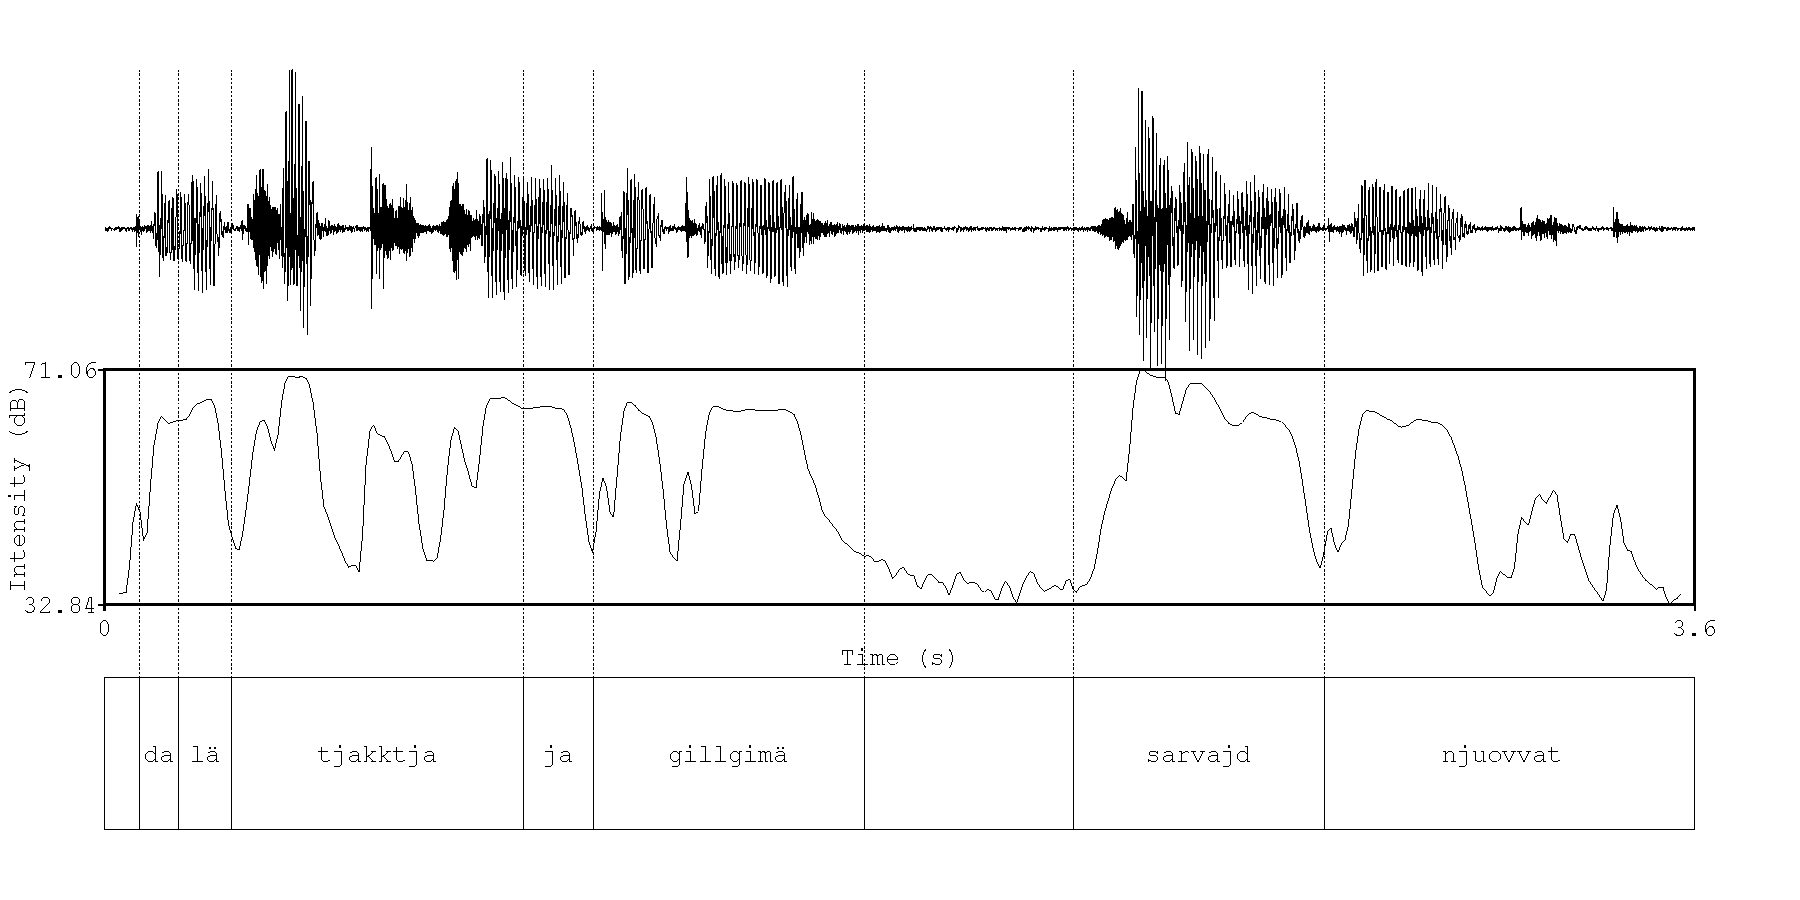
\includegraphics[width=.95\textwidth]{images/pit090826-003.pdf}}
\caption{Waveform and intensity trace illustrating the drop in intensity at the end of an utterance}\label{intonationGraphic}
\end{figure}
Here, the initial syllable nucleus of the first lexical item in the sentence 
\It{tjakttja} has an intensity of 69.7 dB, the other lexical items hover between 63.5 dB and 70.3 dB, while the final lexical item \It{njuovvat} begins at 64 dB on the initial syllable nucleus, and drops abrubtly to 50 dB on the final syllable nucleus. 



\subsection{Utterance-final weakening}\index{prosody!weakening}\label{utteranceFinalDevoicing}
The final two or three syllables of a declarative utterance in \PS\ can be weakened as a way to mark the end of an utterance.\footnote{\It{Arjeplogsmål}, the local Swedish dialect, features a similar phenomenon.} 
This weakening is typically realized by completely devoicing the final one, two or three syllables, often to the point that these are whispered. Alternatively, this can be realized as creaky voice instead of voicelessness. For instance, in the example utterance transcribed in \REF{utteranceFinalDevoicing1} and depicted in the waveform in Figure \vref{utteranceFinalDevoicingGraphic}, devoicing occurs in the final lexical word \It{giesev} ‘summer’, which contains the last two syllables of the utterance. 
The lack of energy in the wave form corresponding to \It{giesev} shows clearly that the word is weakened significantly compared to the rest of the utterance. Note that even the vowels are completely devoiced.

\ea\label{utteranceFinalDevoicing1}%JW: not really good example because ’s’ is voiceless anyway, although the Vs are obviously devoiced - the point is that it’s nearly whispered, which is clearer in the wave-form
\glll	da’l adnam buorak, buorak giesev\\
	t-a=l at̚na-m pʊ͡ɔrakʰ pʊ͡ɔrak k\Bf{ɪ̥͡e̥se̥-v̥}\\
	\Sc{dem}-\Sc{3pl.nom}=be\BS\sc{3pl.prs} have-\sc{prf} good good summer-\sc{acc.sg}\\\nopagebreak
\Transl{they have had a good summer}{} \Corpus{090826}{012}
%\ex\label{utteranceFinalDevoicing1}
%\glll	dä dieda nubbe sábme diehta guk botsoj vuojdnuj\\
%	tɛ tɪ͡eta nupːe saːp̚me tɪ͡eʰta kukʰ poʦoj vʊ͡oj\Bf{j̥t̚n̥ɔ̥j̥}\\
%	then know\BS\sc{2sg.prs} other Saami\BS\sc{nom.sg} know\BS\sc{3sg.prs} how reindeer\BS\sc{nom.sg} look-\sc{3sg.pst}\\
%\Transl{then you know, the other Saami knows what the reindeer looked like}{} \Corpus{100405b.067}
\z
\begin{figure}
\fbox{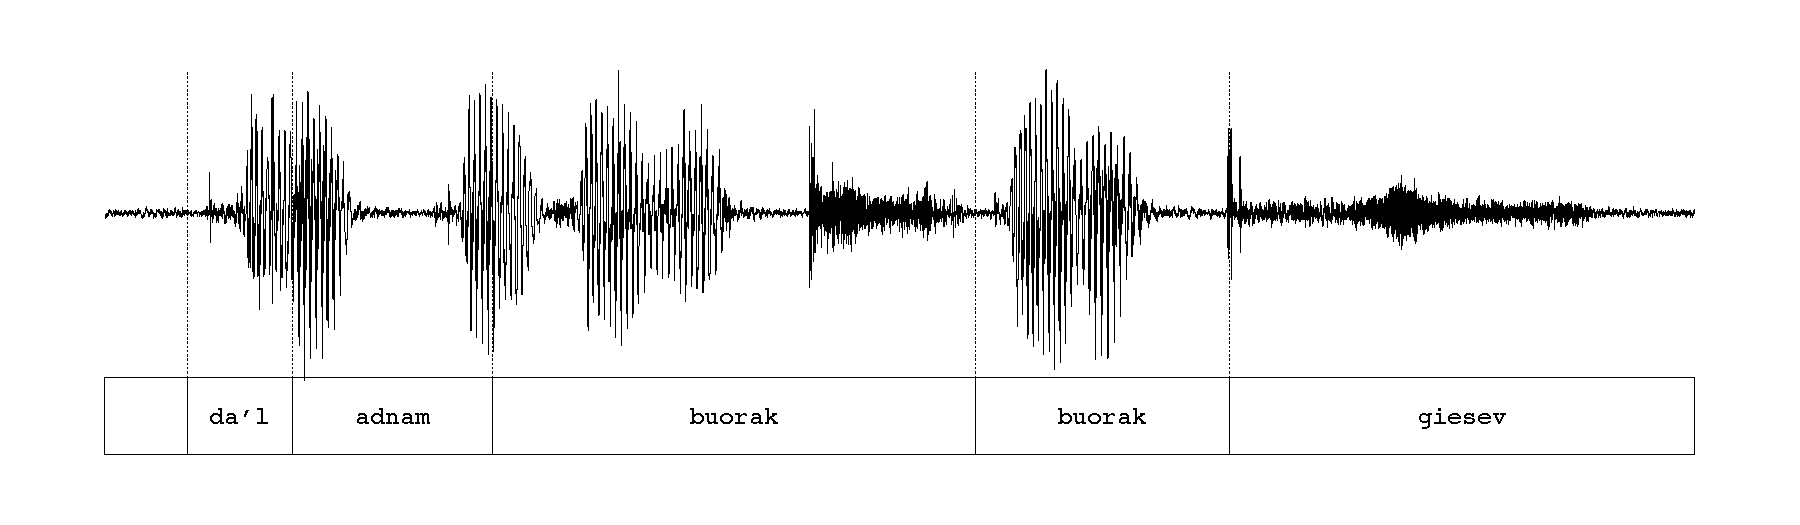
\includegraphics[width=.95\textwidth]{images/pit090826-012.pdf}}
\caption{Waveform illustrating utterance-final weakening}\label{utteranceFinalDevoicingGraphic}
\end{figure}

It is not clear what triggers this devoicing, and future study, particularly looking at the possibility of it being a turn marker in discourse, is needed.



%%%%%%%%%%%%%%%%%%%%%%%%%%%%%% S E G M E N T A L   P H O N O L O G Y %%%%%%%%%%%%%%%%%%%%%%%%%%%%%
%%%%%%%%%%%%%%%%%%%%%%%%%%%%%% S E G M E N T A L   P H O N O L O G Y %%%%%%%%%%%%%%%%%%%%%%%%%%%%%
%%%%%%%%%%%%%%%%%%%%%%%%%%%%%% S E G M E N T A L   P H O N O L O G Y %%%%%%%%%%%%%%%%%%%%%%%%%%%%%
%%%%%%%%%%%%%%%%%%%%%%%%%%%%%% S E G M E N T A L   P H O N O L O G Y %%%%%%%%%%%%%%%%%%%%%%%%%%%%%
%%%%%%%%%%%%%%%%%%%%%%%%%%%%%% S E G M E N T A L   P H O N O L O G Y %%%%%%%%%%%%%%%%%%%%%%%%%%%%%
%%%%%%%%%%%%%%%%%%%%%%%%%%%%%% S E G M E N T A L   P H O N O L O G Y %%%%%%%%%%%%%%%%%%%%%%%%%%%%%
\chapter{Segmental phonology}\index{phonology!consonants}\index{phonology!vowels}\label{csANDvs}
\PS\ has 43 consonant phonemes and 9 vowel phonemes. In the present chapter, the first section (§\,\ref{consonants}) deals with consonants phonemes, their allophonic variation, and consonant clusters. 
The following section (§\,\ref{vowels}) covers vowel phonemes, their allophonic variation, and schwa-epenthesis. 

%\Red{Note that §\,\ref{orthography} provides an overview of the working \PS\ orthography and how it relates to \PS\ phonology. While most of the discussion in this chapter on segmental phonology includes both phonemic and phonetic transcriptions, other chapters only feature the orthographic representation when phonology is not directly relevant. }%moved from intro to Ch. 2, now part of explaining examples in Ch. 1


\section{Consonants}\label{consonants}\index{consonants}\label{CphoneInventory}
The consonant phoneme inventory of Pite Saami can be \marginpar{is the C-inventory too small? better sideways table on single page?}found in Table \vref{Cphonemes}.  
There are plain and preaspirated phonemes for all plosive and affricate positions, and geminate and singleton pairs for all categories. 
Preaspirated, geminate and preaspirated geminate phonemes are restricted to the consonant center position. 
\begin{figure}\centering
%\caption[Consonant phoneme inventory]{Consonant phoneme inventory}\label{Cphonemes}
\resizebox{1\linewidth}{!} {
\begin{tabular}{r c c c c c c c}
\MC{1}{c}{}& \It{bilabial} & \It{labiodental} & \It{alveolar} & \It{post-alveolar} & \It{palatal} & \It{velar} & \MC{1}{c}{\It{glottal}}\\%\cline{2-8}
\It{plosive} & {p ʰp pː ʰpː} &{}& {t ʰt tː ʰtː}&{}&{}&{k ʰk kː ʰkː}&{}\\%6
\It{affricate} &{}&{}& {ʦ ʰʦ ʦː ʰʦː} &{ʧ ʰʧ ʧː ʰʧː}&{}&{}&{}\\%4
\It{fricative} &{}& {f fː v vː} &{s sː}&{ʃ ʃː}&{}&{}&{h}\\%5
\It{nasal} &{m mː}&{}&{n nː} &{}&{ɲ ɲː} & {ŋ ŋː}&{}\\%4
\It{trill}&{}&{}&{r rː}&{}&{}&{}&{}\\%1
\It{approx.}&{}&{}&{l lː}&{}&{j jː}&{}&{}\\%\cline{2-8}%2
%total: 22
\end{tabular}}
\caption[Consonant phoneme inventory]{Consonant phoneme inventory}\label{Cphonemes}
\end{figure}

A description of the consonant phonemes and the distribution of their relevant allophones can be found in §\,\ref{Callophones} for each mode of articulation. 
This is followed by a discussion of consonant clusters. 
For the sake of clarity, the term \It{postaspiration} will be used here to refer to what is commonly referred to simply as \It{aspiration}; this decision also emphasizes the contrast to \It{preaspiration}, which is, in fact, more relevant for Pite Saami than postaspiration.


\subsection{Consonant phonemes and allophonic variations}\label{Callophones}\index{allophony}\index{consonants!allophony}
After a brief note on preaspiration in the following section (§\,\ref{preaspiration}) and a discussion of gemination in §\,\ref{geminateCs}, the consonant phonemes and their allophones are described in the remaining sections (§\,\ref{Plosives} through §\,\ref{oralSonorants}). They are grouped based on manner of articulation.


\subsubsection{Preaspiration}\label{preaspiration}\index{preaspiration}\noindent
In Pite Saami, preaspirated\footnote{As is hopefully evident from this discussion on preaspiration, the term ‘preaspiration’ is not entirely accurate from a phonetic-acoustic point of view since the acoustic correlate of this phenomenon is not actually aspiration in all cases. Nonetheless, there are several reasons to select this term: 1. in the majority of cases, the acoustic correlate is in fact preaspiration, 2. this phonemic phenomenon is often referred to as preaspiration in the literature on %\PS\ \citep{} 
other Saami languages (cf. e.g. \citealt[54-55]{Sammallahti1998} %\citet[15,18]{Svonni2009} %Svonni2009 never defines preasp, just uses the word here and there
or \citealt[57,67]{Feist2010}), and 3. preaspiration can be reconstructed for the half-long and long Proto-Saami plosive and affricate phonemes \citep[cf.][54]{Sammallahti1998} that became the current \PS\ preaspirated phonemes.} 
phonemes only occur in consonant center position. While preaspirated phonemes can be plosives or affricates, the phenomenon that goes along with them is essentially the same. %, and does not interact with the length of the phoneme it is part of. 
The period of aspiration, i.e., the voicelessness preceding the formation of the oral closure, is realized in different ways and depends on the preceding segment. If the preceding segment is a voiced continuant %\marginpar{check for better term than ‘continuant’?} %JW: continuant probably best; Marijn can’t think of a better term
consonant, then the final part of that segment is devoiced. 

While a minimal contrast between a voiceless obstruent preceding a preaspirated consonant phoneme and a voiceless obstruent preceding a plain counterpart phoneme (e.g.: /st/ vs. /sʰt/) is theoretically possible, this cannot be detected because such a consonant cannot be devoiced as it is already voiceless (e.g.: \mbox{/st/\ARROW [st]} and \mbox{/sʰt/\ARROW [st]}). %\footnote{Obstruents never immediately precede /ʰp ʰt ʰk/.} 
When following a high front vowel /i/, preaspiration is realized as a voiceless palatal fricative [ç]. 
In all other cases, preaspiration is a voiceless glottal fricative [h]. This is summarized in Table \vref{preaspRealization}. %on page \pageref{preaspRealization}.
\begin{table}\centering
\caption{The phonetic realizations of preaspiration}\label{preaspRealization}
\begin{tabular}{| c | c | c |}\hline
\It{preceding segment}	& \It{realization of preaspiration}	&\It{example} \\\dline
voiced consonant		& end devoicing of voiced consonant &/mʰp/ \ARROW\ [mm̥p] \\%\hline
%\MC{2}{|c|}{ex.:	/...mʰp.../ \ARROW [...mm̥p...]}\\
\hline
front high vowel /i/		& voiceless palatal fricative [ç]	&/iʰp/ \ARROW\ [içp]\\%\hline
%\MC{2}{|c|}{ex.:	/...iʰp.../ \ARROW [...çp...]}\\
\hline
other vowels			& voiceless glottal fricative [h]	&/aʰp/ \ARROW\ [ahp]\\%\hline
%\MC{2}{|c|}{ex.:	/...aʰp.../ \ARROW [...ahp...]}\\
\hline
\end{tabular}
\end{table}


\subsubsection{Geminates}\label{geminateCs}
The occurrence of geminate consonants is restricted to the consonant center. %and indeed common 
As illustrated in Table \vref{Cphonemes}, only the glottal fricative /h/ does not have a comparable geminate phoneme. %In such cases, the two phonemes are realized together as a geminate. 
Geminate segments are realized with a longer overall duration than the corresponding singleton phonemes. This observation is based not only on speakers’ observations that such sounds are ‘longer’, but also on my own observations and analyses, including an acoustic-phonetic comparison of duration in geminate phonemes; cf.\,§\,\ref{plosiveDurationComparison} for a detailed comparison non-voiced plosive durations in the consonant center. 

For plosives and affricates, only one stop closure is formed, and the overall duration of the stop closure is longer than the duration of a corresponding single consonant. Some examples are provided in \REF{outside} through \REF{motherNOMSG}.
\PhonGlossWL{outside}{ta\Bf{pː}en}{ta\Bf{pː}en}{dabben}{\Sc{dem}\BS\Sc{iness.sg}}{3672}
\PhonGloss{ribbonNOMSG}{pa\Bf{tː}e}{pa\Bf{tː}e}{badde}{ribbon\BS\Sc{nom.sg}}{080701b}{.082}%{swadesh?}
\PhonGloss{windNOMSG1}{pɛ\Bf{kː}a}{pɛ\Bf{kː}a}{bägga}{wind\BS\Sc{nom.sg}}{080702b}{.067}%{swadesh?}
\PhonGlossWL{goINF}{vaː\Bf{ʦː}e-t}{va:\Bf{tːs}etʰ}{vádtset}{go-\Sc{inf}}{2049}
\PhonGlossWL{motherNOMSG}{ʧi\Bf{ʧː}e}{ʧi\Bf{tːʃ}e}{tjidtje}{mother\BS\Sc{nom.sg}}{3618}

Preaspirated plosive and affricate geminates also exist. %the first segment can be preaspirated, in which case, the period of preaspiration tends to be longer than for a single preaspirated segment not followed by the corresponding homorganic plosive or affricate. %Similarly, a preaspirated plosive or affricate can be followed by the corresponding plain plosive or affricate. 
In such cases, the duration of both the preaspiration phase and the following stop closure are longer than in the corresponding preaspirated single consonants. Some examples are found in \REF{cleverPREDSG} through \REF{fatherNOMSGb}.
\PhonGloss{cleverPREDSG}		{ʧɛ\Bf{ʰpː}e}		{ʧɛ\Bf{hpː}e}		{tjähppe}	{clever\BS\Sc{pred.sg}}		{090930b}{.077}
%\PhonGloss{milkingbowlNOMSG}	{naː\Bf{ʰpp}e}	{naː\Bf{hpː}e}	{náhppe}	{milking\_cup\BS\Sc{nom.sg}}	{080621}
\PhonGloss{canINF}				{maː\Bf{ʰtː}e-t}	{maː\Bf{htː}etʰ}	{máhttet}	{can-\Sc{inf}}			{080926}{.03m21s}
%\PhonGloss{wolfNOMSG}			{kum\Bf{ʰpp}e}	{kum\Bf{m̥pː}e}	{gummpe}	{wolf\BS\Sc{nom.sg}}		{0671}
%\PhonGloss{workINF}			{par\Bf{ʰkk}at}	{par\Bf{r̥kː}atʰ}	{barrgat}	{work-\Sc{inf}}			{101208.005}
\PhonGlossWL{turnAround3SGPST}{ma:\Bf{ʰʦː}a-j}{ma:\Bf{htːs}aj}{máhttsaj}{turn.around-\Sc{3sg.pst}}{6613}
\PhonGlossWL{fatherNOMSGb}{a:\Bf{ʰʧː}e}{a:\Bf{htːʃ}e}{áhttje}{father\BS\Sc{nom.sg}}{0016}

For all other consonants, the overall duration of a geminate is longer than for the corresponding singleton consonant. Examples of such geminates are provided in \REF{areaNOMSG} through \REF{letINF}.
\PhonGlossWL{areaNOMSG}	{taː\Bf{fː}o}	{taː\Bf{fː}o}	{dáffo}	{area\BS\Sc{nom.sg}}		{2367}%
%\PhonGloss{rapids}	{raː\Bf{ff}e}	{raː\Bf{fː}e}	{ráffe}	{rapids\BS\Sc{nom.sg}}		{2713}%
\PhonGlossWL{peaceNOMSG}	{raː\Bf{vː}e}	{raː\Bf{vː}e}	{rávve}	{peace\BS\Sc{nom.sg}}		{1366}%
\PhonGlossWL{partNOMSG}	{ɔ\Bf{sː}e}	{ɔ\Bf{sː}e}	{åsse}	{part\BS\Sc{nom.sg}}	{2269}
\PhonGlossWL{horsetailNOMSG}	{ɔ\Bf{ʃː}e}	{ɔ\Bf{ʃː}e}	{åssje}	{horsetail\BS\Sc{nom.sg}}	{2270}
\PhonGloss{suck3SGPRS}{ɲa\Bf{mː}a}{ɲa\Bf{mː}a}{njamma}{suck\BS\Sc{3sg.prs}}{080701b}{.005a}
\PhonGlossWL{littleBitNOMSG}{pi\Bf{nː}a}{pi\Bf{nː}a}{binna}{little.bit\BS\Sc{nom.sg}}{2446}
%\PhonGloss{eggNOMSG}{mɔ\Bf{nn}e}{mɔ\Bf{nː}e}{månne}{egg\BS\Sc{nom.sg}}{080621}
\PhonGloss{daughterInLawNOMSG}{ma\Bf{ɲː}e}{ma\Bf{ɲː}e}{mannje}{daughter.in.law\BS\Sc{nom.sg}}{080621}{.74m04s}
%\PhonGlossLongGloss{daughterInLawNOMSG}{ma\Bf{ɲː}e}{ma\Bf{ɲː}e}{mannje}{daughter\_in\_law\BS\Sc{nom.sg}}{080621}{.74m04s}
\PhonGloss{after}{ma\Bf{ŋː}el}{ma\Bf{ŋː}el}{maŋŋel}{after}{080924}{.529}
\PhonGlossWL{iceOverINF}{kɔ\Bf{rː}oti-t}{kɔ\Bf{rː}otɪtʰ}{gårrodit}{ice.over-\Sc{inf}}{4693}
\PhonGlossWL{fireNOMSG}{tɔ\Bf{lː}ɔ}{tɔ\Bf{lː}ɔ}{dållå}{fire\BS\Sc{nom.sg}}{0421}%KORRECTED from NOM:PL to SG -- 18.09.2013
\PhonGlossWL{letINF}{paː\Bf{jː}a-t}{paː\Bf{jː}atʰ}{bájjat}{let-\Sc{inf}}{3439}

Due mostly to the nature of morphophonemic stem alternations, there are numerous minimal pairs differing only in the presence of a singleton versus a geminate consonant; cf. §\,\ref{Cgrad} on consonant gradation for examples. %, and the series of two identical segments has often been treated as a phonemic geminates or as morphologically triggered gemination in the literature on both \PS\ and other Saami languages with similar phenomena (cf. \cite{Lehtiranta1992}:46-47; \cite{Sammallahti1998}:46-50; ). 

It is also possible to have geminate fricative or sonorant phonemes, as described above, followed by a plosive of affricate phoneme, as illustrated by the examples in \REF{tableNOMSG} through \REF{tightPREDSG}.
\PhonGlossWL{tableNOMSG}	{pɛ\Bf{vː}te}	{pɛ\Bf{vː}te}	{bävvde}	{table\BS\Sc{nom.sg}}		{0289}%
\PhonGlossWL{rapidsNOMSG}	{lu\Bf{sː}pe}	{lu\Bf{sː}pe}	{lusspe}	{rapids\BS\Sc{nom.sg}}		{1077}%
\PhonGlossWL{shall3SGPRS}	{ka\Bf{lː}ka}	{ka\Bf{lː}ka}	{gallga}	{will\BS\Sc{3sg.prs}}		{6626}%
\PhonGlossWL{tightPREDSG}	{kaː\Bf{rː}ʰʧe}	{kaː\Bf{rr̥}ʧe}	{gárrtje}	{tight\BS\Sc{pred.sg}}		{0554}%

A series of two identical consonant phonemes can arise at the internal stem boundary of a compound. In such cases, the resulting duration can be longer than for a single plosive, but is not necessarily so, as the two phonemes are often realized as a singleton, as in \REF{cervicalVertebraeNOMSG}.
\PhonGlossWL{cervicalVertebraeNOMSG}{ʧepo\Bf{t}\PLUS\Bf{t}a:k:te}{ʧi͡epo\Bf{t}a:kʰte}{tjiebotdákkte\footnotemark}{cervical.vertebra\BS\Sc{nom.sg}}{3771}
%\PhonGlossLong{cervicalVertebraeNOMSG}{ʧepo\Bf{t}\PLUS\Bf{t}a:k:te}{ʧi͡epo\Bf{t}a:kʰte}{tjiebotdákkte\footnotemark}{cervical\_vertebra\BS\Sc{nom.sg}}{}{3771}
\footnotetext{The word \It{tjiebotdákkte} literally means ‘throat-bone’, cf. \It{tjiebot} ‘throat’ and \It{dákkte} ‘bone’.}
Due to the morpheme boundary separating such segments, it is clear that this is not a case of a geminate phoneme, even if the realization may resemble that of a geminate. 


\subsubsection{Plosives}\label{Plosives}\index{consonants!plosives}%%%%%%%% PLOSIVES %%%%%%%%%%%%%%%
The plosive series in Pite Saami consists of the phonemes and their phonetic realizations shown in Figure \vref{PlosivePhonemes}. The distribution of the allophones will be discussed here. As all three relevant places of articulation behave in much the same way, the various manners of articulation for each place will be treated together.
\begin{figure}\begin{center}
\begin{tabular}{c c l}
/p/ &:& [p] [pʰ] [p̚\,] \\ %should be written with <b>
/pː/ &:& [pː] \\ %should be written with <bb>
/ʰp/ &:& [hp] [ ̥p] [çp]  \\ %should be written with <hp>
/ʰpː/ &:& [hpː] \\ %should be written with <hpp>
%/b/ &:& [b] \\ %only loans (?)
/t/ &:& [t] [tʰ] [t̚\,] \\%unreleased even before palatal (see butter.sg.nom)! probably just +CORONAL
/tː/ &:& [tː] \\
/ʰt/ &:& [ht] [ ̥t] [çt] \\
/ʰtː/ &:& [htː] \\
%/d/ &:& [d] \\ %only loans (?)
/k/ &:& [k] [kʰ] [k̚\,] \\
/kː/ &:& [kː] \\
/ʰk/ &:& [hk] [ ̥k] [çk]  \\
/ʰkː/ &:& [ʰkː] \\
%/g/ &:& [g] \\ %only loans (?)
\end{tabular}
\end{center}
\caption{Plosive and affricate phonemes and their realizations}\label{PlosivePhonemes}
\end{figure}


\paragraph{Voiceless singleton plosives /p\,t\,k/}\label{ptk}
The segments /p\,t\,k/ are bilabial, alveolar and velar (respectively) voiceless singleton plosive phonemes. %With the exception of their individual places of articulation, they essentially exhibit the same behavior and will be described together here. %JW: redundant, see previous paragraph
The voiceless singleton plosives can occur in all prosodic consonant positions and are subject to allophonic variation, depending on the prosodic environment. In syllable-onset position, a plain (unaspirated) voiceless plosive [p\,t\,k] is produced, as seen in examples \REF{dogNOMSG} through \REF{goodADV1}. %\footnote{In these and the examples in the following sections on other consonant and vowel phonemes, the underlying phonological representation, the phonetic form, the orthographic form, the gloss, and the source of the phonetic form are listed for each instance and in that order. The relevant phones and phonemes are in bold face.}
\PhonGloss{dogNOMSG}{\Bf{p}ena}{\Bf{p}i͡ena}{bena}{dog\BS\Sc{nom.sg}}{090926}{.057}
\PhonGloss{wish3DUPRS}{saːvːa-\Bf{p}a}{saːʋːa\Bf{p}aʰ}{sávvabah}{wish-\Sc{3du.prs}}{100323a}{.060}
\PhonGloss{2SGNOM}{\Bf{t}ɔj}{\Bf{t}ɔj}{dåj}{\Sc{2sg.nom}}{100323a}{.014}
\PhonGloss{cheeseNOMPL}{vos\Bf{t}a}{ʋu͡ɔs\Bf{t}a}{vuosta}{cheese\BS\Sc{nom.pl}}{080917c}{.09m47s}
\PhonGloss{widePREDSG}{\Bf{k}op\Bf{t}ok}{\Bf{k}opʰ\Bf{t}okʰ}{gåbdåk}{wide\BS\Sc{pred.sg}}{091001}{.035}
\PhonGloss{drink1SGPRS}{ju\Bf{k}a-v}{jʊ\Bf{k}ɑʋ}{jugav}{drink-\Sc{1sg.prs}}{100323a}{.115}
\PhonGloss{goodADV1}{\Bf{p}ora-\Bf{k}it}{\Bf{p}u͡ora\Bf{k}ɪtʰ}{buoragit}{good-\Sc{advz}}{100323a}{.213}
%\PhonGloss{queenNOMSG}{\Bf{t}rotnək}{\Bf{t}rot̚nɘkʰ}{drodnik\footnotemark}{queen.\Sc{nom.sg}}{missing}
%\footnotetext{from Swedish \It{drottning}}
%\PhonGloss{icecreamNOMSG}{\Bf{k}laːsːa}{\Bf{k}laːsːa}{glássa\footnotemark}{ice\_cream.\Sc{nom.sg}}{missing}
%\footnotetext{from Swedish \It{glass} (<French \It{glace})}

The plain voiceless singleton pronunciations [p\,t\,k] %\marginpar{mention that {[k]} is farther back in velar position (sounds almost uvular) than in English/German/Swedish?} 
are also found in consonant clusters in word-onset position, an environment usually found in recent and older loan words from (North) Germanic, as in examples \REF{queenNOMSG} and \REF{icecreamNOMSG}. %
%\PhonGloss{queenNOMSG}{\Bf{t}rotnik}{\Bf{t}rot̚nikʰ}{drodnik}{queen\BS\Sc{nom.sg}}{missing}%\footnotetext{from Swedish \It{drottning}.}
%\PhonGloss{icecreamNOMSG}{\Bf{k}laːsːa}{\Bf{k}laːsːa}{glássa}{ice\_cream\BS\Sc{nom.sg}}{missing}%\footnotetext{from Swedish \It{glass} (<French \It{glace}).}
\PhonGlossWL{queenNOMSG}{\Bf{t}rotnik}{\Bf{t}rot̚\,nikʰ}{drodnik\footnotemark}{queen\BS\Sc{nom.sg}}{0377}\footnotetext{From Swedish \It{drottning}.}
\PhonGlossWL{icecreamNOMSG}{\Bf{k}laːsːa}{\Bf{k}laːsːa}{glássa\footnotemark}{ice.cream\BS\Sc{nom.sg}}{0529}\footnotetext{From Swedish \It{glass} (<French \It{glace}).}

The voiceless singleton plosives phonemes are postaspirated word-finally\footnote{Note, however, that speakers from the northern parts of \PS\ territory tend to voice the voiceless plosives phonemes as [b d g] in word-final position.} 
as [pʰ\,tʰ\,kʰ], as in examples \REF{be1PLPRS} through \REF{alonePRED}, as in examples \REF{alonePRED} through \REF{whoopingCoughNOMSG}. This is also the case across an internal compound boundary, as in \REF{whoopingCoughNOMSG}.\footnote{The word \It{båktjanitgåssås} in \REF{whoopingCoughNOMSG} refers to the whooping cough, and is a compound composed of \It{båktjanit} ‘to suffocate’ and \It{gåssås} ‘cough’.}
 %\marginpar{check if this is true at internal border of compounds or before nonhomorganic nasal? also check grade of ex. \REF{hairNOMPL} and \REF{marshNOMSG} - maybe this is true for all phonemic lengths!}%maybe also at the internal word-border of a compound (but what are the criteria for compounds then?); maybe also before a nonhomorganic nasal?
\PhonGloss{be1PLPRS}{orːo-\Bf{p}}{orːo\Bf{pʰ}}{årrop}{be-\Sc{1pl.prs}}{100323a}{.158}
\PhonGloss{goodADV2}{pora-ki\Bf{t}}{pʊ͡ɔrakɪ\Bf{tʰ}}{buoragit}{good-\Sc{advz}}{100323a}{.213}
\PhonGloss{alonePRED}{ikto\Bf{k}}{ikʰto\Bf{kʰ}}{iktuk}{alone}{100323a}{.169}
%\PhonGloss{marshNOMSG}{kɔ\Bf{tː}kɔ}{kɔ\Bf{tʰ}kːɔ}{gåttkå}{marsh\BS\Sc{nom.sg}}{}{0762}%check if this is grade I
%\PhonGlossLong{1}{2}{3}{4}{5}{6}
\PhonGlossWL{whoopingCoughNOMSG}{pɔ\Bf{kʧ}ani\Bf{t}\PLUS\Bf{k}ɔs:ɔs}{pɔ\Bf{kʰʧ}ani\Bf{tʰk}ɔs:ɔs}{båktjanitgåssås}{whooping.cough\BS\Sc{nom.sg}}{5993}
%\PhonGlossLong{whoopingCoughNOMSG}{pɔ\Bf{kʧ}ani\Bf{t}\PLUS\Bf{k}ɔs:ɔs}{pɔ\Bf{kʰʧ}ani\Bf{tʰk}ɔs:ɔs}{båktjanitgåssås\footnotemark}{whooping\_cough\BS\Sc{nom.sg}}{}{5993}
%\footnotetext{The word \It{båktjanitgåssås} refers to the whooping cough, and is a compound composed of \It{båktjanit} ‘to suffocate’ and \It{gåssås} ‘cough’.}

When preceding a non-homorganic plosive or affricate, a short aspiration occurs between the two segments, as in \REF{hairNOMPL} or in \REF{alonePRED} above. 
\PhonGloss{hairNOMPL}{vo\Bf{p}ta}{ʋu͡o\Bf{p}ʰta}{vuopta}{hair\BS\Sc{nom.pl}}{080701b}{.092}%check if this is grade I

For all three plosive singleton phonemes, the closure is not released when a homorganic consonant %sonorant 
follows; they are then realized as [p̚ t̚ k̚\,]. Word-internally, this situation is only found in the consonant center and with a homorganic sonorant, as shown in examples \REF{heartNOMSG1} through \REF{butterNOMSG}. 
\PhonGloss{heartNOMSG1}{vaːj\Bf{p}mo}{ʋaːj\Bf{p̚}mo}{vájbmo}{heart\BS\Sc{nom.sg}}{080701b}{.115}
\PhonGloss{have2DUIMP}%different example here for unreleased alveolar voiceless plosive before another alveolar C!
{e\Bf{t}ni-t}{e\Bf{t̚}nɪtʰ}{ednit}{have-\Sc{2du.imp}}{100323a}{.251}
\PhonGloss{iceNOMSG}{je\Bf{k}ŋa}{je\Bf{k̚}ŋa}{jegŋa}{ice\BS\Sc{nom.sg}}{080702b}{.070}
\PhonGloss{butterNOMSG}{vo\Bf{t}ja}{vʊ͡ɔ\Bf{t̚}ja}{vuodja}{butter\BS\Sc{nom.sg}}{080926}{.01m15s} %Check this transcription!
%\PhonGloss{be3PLPSTa}{li\Bf{t}jin}{li\Bf{t̚}jɪn}{lidjen}{be-\Sc{3pl.pst}}{081011.049}%JW: decided this example isn’t necessary, plus it’s a big weird b/c it’s listed as lijjin in the worlist
%\PhonGlossLong{cervicalVertebraeNOMSG}{ʧepo\Bf{t}\PLUS\Bf{t}a:k:te}{ʧi͡epo\Bf{t}a:kʰte}{tjiebotdákkte\footnotemark}{cervical\_vertebra\BS\Sc{nom.sg}}{3771}
%\footnotetext{\It{tjiebotdákkte} is a cervical vertebra, literally \It{tjiebot} ‘throat’ and \It{dákkte} ‘bone’.}


\paragraph{Voiceless geminate plosives /pː\,tː\,kː/}
The segments /pː\,tː\,kː/ are bilabial, alveolar and velar (respectively) geminate plosive phonemes. They are very restricted in their distribution as they only occur in the consonant center %(cf. §\,\ref{CCent}) % in the literature on Saami languages, but this refers to morphophonological status, which I try to avoid here in this purely phonological description. One could also refer to this position in terms of feet; then, Pite Saami would have trochaic feet counting from the left, in which case the geminate plosive phonemes only occur foot-internally.}
and never occur word-initially or word-finally. %In speech, the oral closure of these phonemes tends to have a duration of between 200 and 300 milliseconds.\marginpar{does this need more solid statistical evidence?}
Examples for the geminate plosive phonemes can be found in examples \REF{there} through \REF{windNOMSG1b}.
\PhonGlossWL{there}{to\Bf{pː}en}{to\Bf{pː}en}{dobben}{yonder}{3581}
\PhonGloss{ribbonNOMSGb}{pa\Bf{tː}e}{pa\Bf{tː}e}{badde}{ribbon\BS\Sc{nom.sg}}{090930a}{.215}
\PhonGloss{windNOMSG1b}{pɛ\Bf{kː}a}{pɛ\Bf{kː}a}{bägga}{wind\BS\Sc{nom.sg}}{080621}{.77m27s}

When preceding a non-homorganic plosive or affricate, a short aspiration occurs between the two segments, as in \REF{bayNOMSG1}. 
\PhonGloss{bayNOMSG1}{lu͡a\Bf{kː}ta}{lʊ͡a\Bf{kː}ʰta}{luakkta}{bay\BS\Sc{nom.sg}}{080917c}{.03m51s}

%%%%These are examples for /ʰp ʰt ʰk/!!!
%\begin{exe}
%\PhonGloss{milkingbowlNOMPL}%not relevant for /pː/!
%\begin{tabular}{p{2cm} p{2cm} p{1.5cm} p{4cm} l}
%/naː\Bf{ʰp}e}{naː\Bf{ʰp}ɘ}{náhpe} &'milking\_cup-\Sc{nom.pl}}{080621}
%\end{tabular}
%\PhonGloss{want3SGPRS}
%\begin{tabular}{p{2cm} p{2cm} p{1.5cm} p{4cm} l}
%[si\Bf{ʰt}a}{si\Bf{tː}a}{sihta} &'want.\Sc{3sg.prs}}{080926}
%\end{tabular}
%\PhonGloss{drinkINF}
%\begin{tabular}{p{2cm} p{2cm} p{1.5cm} p{4cm} l}
%[ju\Bf{ʰk}atʰ}{ju\Bf{kː}at}{juhgat} &'drink-\Sc{inf}}{100323a.114}
%\end{tabular}
%\end{exe}


\paragraph{Preaspirated singleton plosives /ʰp\,ʰt\,ʰk/}
%\paragraph[Preaspirated singleton plosives \\/ʰp ʰt ʰk/]{Preaspirated singleton plosives /ʰp ʰt ʰk/}
The segments \mbox{/ʰp\,ʰt\,ʰk/} are preaspirated bilabial, alveolar and velar (respectively) singleton plosive phonemes. They are only licensed as the sole consonant or the final consonant segment in the consonant center. 
The phonetic realization of preaspiration depends on the preceding phoneme, as described in §\,\ref{preaspiration}. 
Examples can be found in \REF{milkingbowlNOMPL} through \REF{louseNOMSG}. 
\PhonGloss{milkingbowlNOMPL}	{naː\Bf{ʰp}e}		{naː\Bf{hp}e}	{náhpe}	{milking.cup\BS\Sc{nom.pl}}	{080621}{.55m16s}
\PhonGloss{houseNOMSGb}		{tɔ\Bf{ʰp}e}		{tɔ\Bf{hp}e}		{dåhpe}	{house\BS\Sc{nom.sg}}		{100310b}{.083}
\PhonGloss{towardsNorth}		{nurː\Bf{ʰt}as}	{nur\Bf{r̥t}as}	{nurrtas}	{towards.the.north}		{081011}{.177}
\PhonGloss{thankACCSG}		{kij\Bf{ʰt}o-v}		{kij\Bf{j̥t}oʋ}		{gijtov}	{thank-\Sc{acc.sg}}		{080621}{.11m45s}
\PhonGlossWL{louseNOMSG}		{ti\Bf{ʰk}e}		{ti\Bf{çk}e}		{dihke}	{louse\BS\Sc{nom.sg}}		{2359}

\paragraph{Preaspirated geminate plosives /ʰpː\,ʰtː\,ʰkː/}
%\paragraph[Preaspirated geminate plosives \\/ʰpː ʰtː ʰkː/]{Preaspirated geminate plosives /ʰpː ʰtː ʰkː/}
The segments \mbox{/ʰpː\,ʰtː\,ʰkː/} are preaspirated bilabial, alveolar and velar (respectively) geminate plosive phonemes. 
They are only licensed as the sole consonant in the consonant center.  
Examples can be found in \REF{cleverPREDSGb} through \REF{canINFb}; cf. §\,\ref{preaspiration} on allophonic variation in preaspiration. 
\PhonGloss{cleverPREDSGb}		{ʧɛ\Bf{ʰpː}e}		{ʧɛ\Bf{hpː}e}		{tjähppe}	{clever\BS\Sc{pred.sg}}		{090930b}{.077}
\PhonGloss{milkingbowlNOMSGb}	{naː\Bf{ʰpː}e}	{naː\Bf{hpː}e}	{náhppe}	{milking.cup\BS\Sc{nom.sg}}	{080621}{.54m38s}
\PhonGloss{canINFb}			{maː\Bf{ʰtː}e-t}	{maː\Bf{htː}etʰ}	{máhttet}	{can-\Sc{inf}}			{080926}{.03m21s}
%% the following two are actually geminate sonorants+singleton-plosive!!
%\PhonGlossWL{wolfNOMSG}			{kum\Bf{ʰpː}e}	{kum\Bf{m̥pː}e}	{gummpe}	{wolf\BS\Sc{nom.sg}}		{0671}
%\PhonGloss{workINF}			{par\Bf{ʰkː}a-t}	{par\Bf{r̥kː}atʰ}	{barrgat}	{work-\Sc{inf}}			{101208}{.005}


\paragraph[Non-voiced plosive durations in the consonant center]{Comparison of non-voiced plosive durations in the consonant center}\label{plosiveDurationComparison}
While a thorough study of length phenomena in \PS\ is beyond the scope of the current study, it is worth noting the actual duration which the various plosive phonemes are realized with in the consonant center. %\footnote{The consonant center is the only position in which all plosive and affricate phonemes occur.}%JW: footnote not relevant!
Specifically, %\marginpar{add praat illustrations for these, at the latest for the final/print version} %JW: not worth it, wouldn’t really show much anyway, durations sufficient!
a plain geminate plosive and a singleton preaspirated plosive have approximately the same duration for the period of stop closure (around 300ms), and are at least 100ms longer than plain singleton plosives and 100ms shorter than a preaspirated geminate plosive. In this respect, plain geminate plosives and preaspirated singleton phonemes seem to group together concerning stop closure duration. 
%, plain singletons are significantly shorter than preaspirated singletons, and plain geminates are significantly shorter than preaspirated geminates. 
Table \vref{stopClosureComparision} %on page \pageref{stopClosureComparision} 
shows some (near) minimal sets and duration measurements as a comparison. However, this alignment seems to be irrelevant phonologically. 

\begin{table}\centering
\caption[Comparison of stop closure durations]{Minimal sets or near minimal sets for comparison of stop closure durations (in milliseconds) for plain and preaspirated singletons and geminates}\label{stopClosureComparision}
\resizebox{\columnwidth}{!}{%
\begin{tabular}{|c | c | c | c | c |}\cline{2-5}%\hline
\MC{1}{c|}{}	&\It{plain single}		& \It{plain geminate} 		&\It{preasp. single}			&\It{preasp. geminate}\\%\dline%\multirow{2}{*}{\It{preasp. geminate}\\
\MC{1}{c|}{}	&/p/					& /pː/					& /ʰp/					& /ʰpː/ \\\cline{2-5}
\MC{1}{c|}{}	&145-150ms			&320-340ms			&280-340ms				&460-490ms\\\cline{2-5}%\hline
\MC{1}{c|}{}	&\It{short}				&\MC{2}{c|}{\It{medium}}							&\It{long}	\\\hline
\MR{4}{*}{\begin{sideways}\It{set 1}\end{sideways}}	
			&tɔ\Bf{p}e				& tu\Bf{pː}en			& tɔ\Bf{hp}e				& tɔ\Bf{hpː}o\\
%			&tɔ.\Bf{p}e			& tu\Bf{p.p}en			& tɔ\Bf{ʰ.p}e				& tɔ\Bf{ʰp.p}o\\%JW: here with syllable boundaries!
			&150ms				&320ms				& 340ms					&490ms\\
			&house\BS\Sc{gen.sg}	&outside				&house\BS\Sc{nom.sg}		&sheath\BS\Sc{nom.sg}\\
			&\hyperlink{pit100310b}{\small[pit100310b]}		& \small[3581]	&\hyperlink{pit100310b}{\small[pit100310b]}			& \small[3627]\\\hline
\MR{4}{*}{\begin{sideways}\It{set 2}\end{sideways}}
			&naː\Bf{p}erti-t			&nu\Bf{pː}e			& naː\Bf{hp}e				& naː\Bf{hpː}e\\
%			&naː\Bf{.p}er.ti-t			&nu\Bf{p.p}e			& naː\Bf{ʰ.p}e				& naː\Bf{ʰp.p}e\\%JW: here with syllable boundaries!
			&145ms				&340ms				&280ms					&460ms\\
			&drill-\Sc{inf}			&other				&milking.bowl\BS\Sc{nom.pl}	&milking.bowl\BS\Sc{nom.sg} \\
			&\small[3378]	&\small[1317]	&\hyperlink{pit080917a}{\small[pit080917a]}		&\hyperlink{pit080917a}{\small[pit080917a]} \\\hline%\cline{2-5}
%			&145-150ms			&\MC{2}{c||}{280-340ms}							&460-490ms\\\hline
%\MC{1}{c|}{}	&\It{short				&\MC{2}{c|}{\It{medium}							&\It{long	\\\cline{2-5}
\end{tabular}}
\end{table}

\FloatBarrier

%%%%%%%% AFFRICATES %%%%%%%%%%%%%%%
%%%%%%%% AFFRICATES %%%%%%%%%%%%%%%
\subsubsection{Affricates}\label{Affricates}\index{consonants!affricates}
The affricate series in Pite Saami consists of the phones and their phonetic realizations shown in Figure \vref{AffricatePhonemes}. As affricates, they begin as a plosive stop, which is then released into a sibilant fricative. %They very closely resemble the plosive series, as discussed above in §\,\ref{Plosives}, in their phonotactic restrictions. %\marginpar{or just include these with the regular plosives?}
These are described below.
\begin{figure}\centering
\begin{tabular}{c c l}
/ʦ/ &:& [ʦ] \\ %should be written as <ts>
/ʦː/ &:& [tːs] \\ %should be written as <hts>
/ʰʦ/ &:& [hʦ] [ ̥ʦ] [çʦ] \\ %should be written as <hhts>
/ʰʦː/ &:& [htːs] \\ %should be written as <hhts>
/ʧ/ &:& [ʧ] \\ %should be written as <ts>
/ʧː/ &:& [tːʃ] \\ %should be written as <hts>
/ʰʧ/ &:& [hʧ] [ ̥ʧ] [çʧ]  \\ %should be written as <hhts>
/ʰʧː/ &:& [htːʃ] \\ %should be written as <hhts>
\end{tabular}
\caption{Affricate phonemes and their realizations}\label{AffricatePhonemes}
\end{figure}

\paragraph{Plain singleton affricates /ʦ\,ʧ/}\label{tstj}
\marginpar{No BOLD for ʦ ligature!}The segments /ʦ\,ʧ/ are unvoiced alveolar and postalveolar (respectively) singleton affricate phonemes. Both can occur in syllable onset position. Examples can be found in \REF{peeINF} through \REF{wringINF}.
\PhonGlossWL{peeINF}{\Bf{ʦ}isːa-t}{\Bf{ʦ}isːatʰ}{tsissat}{pee-\Sc{inf}}{3700}
\PhonGlossWL{reindeerNOMSG}{pɔ\Bf{ʦ}oj}{pɔ\Bf{ʦ}oj}{båtsoj}{reindeer\BS\Sc{nom.sg}}{0263}
\PhonGlossWL{waterGENSG}{\Bf{ʧ}aː\Bf{ʦ}e-v}{\Bf{ʧ}aː\Bf{ʦ}ev}{tjátsev}{water-\Sc{gen.sg}}{1861}
\PhonGlossWL{wringINF}{pɔ\Bf{ʧ}esti-t}{pɔ\Bf{ʧ}estitʰ}{båtjestit}{wring-\Sc{inf}}{0262}%probably a derivation of båhtjet - ‘milk’!

The postalveolar affricate /ʧ/ can also occur in word-final\footnote{There is one particle \It{guts} with the alveolar affricate in final position, but it is not clear what this is or whether it is /ʦ/ or /tʦ/ in the consonant center (it is spelled inconsistently, as well). Noticeably, it is monosyllablic, and could be an abbreviated form of a typical bisyllabic word which has been lexicalized in its rapid-speech form, in which case it was historically in word-medial position.} % but the second syllable is lost in rapid speech in this particular phrase.} 
position, frequently as the diminutive suffix \It{-tj}, as in \REF{dogDIM}.
\PhonGlossWL{dogDIM}{petnaka-\Bf{ʧ}}{pet̚naka\Bf{ʧ}}{bednagatj}{dog-\Sc{dim}\BS\Sc{nom.sg}}{5717}

\paragraph{Plain geminate affricates /ʦː\,ʧː/}
The segments /ʦː\,ʧː/ are unvoiced alveolar and postalveolar (respectively) geminate affricate phonemes. As with all other geminates, the affricate geminates only occur in the consonant center. The duration of the stop closure is longer in geminate affricates compared to their singleton affricate counterparts, while the duration of the fricative element is not relevant.
Examples can be found in \REF{goINFb} and \REF{motherNOMSGb}.
\PhonGlossWL{goINFb}{vaː\Bf{ʦ:}e-t}{va:\Bf{tːs}etʰ}{vádtset}{go-\Sc{inf}}{2049}
\PhonGlossWL{motherNOMSGb}{ʧi\Bf{ʧ:}e}{ʧi\Bf{tːʃ}e}{tjidtje}{mother\BS\Sc{nom.sg}}{3618}

\paragraph{Preaspirated singleton affricates /ʰʦ\,ʰʧ/}
%\paragraph[Preaspirated singleton affricates \\/ʰʦ ʰʧ/]{Preaspirated singleton affricates /ʰʦ ʰʧ/}
The segments \mbox{/ʰʦ\,ʰʧ/} are preaspirated alveolar and postalveolar (respectively) singleton affricate phonemes. Just as with the preaspirated plosives, the preaspirated affricates only occur as the sole consonant or the final consonant in the consonant center. 
The phonetic realization of preaspiration depends on the preceding phoneme, as described in §\,\ref{preaspiration}. 
Examples can be found in \REF{reindeerNOMPL} through \REF{henNOMSG}.
\PhonGloss{reindeerNOMPL}{pu\Bf{ʰʦ}u}{pu\Bf{hʦ}u}{buhtsu}{reindeer\BS\Sc{nom.pl}}{110413b}{.085}
%\PhonGloss{waterNOMSG}{ʧaː\Bf{ʰʦ}e}{ʧaː\Bf{hʦ}e}{tjáhtse}{water\BS\Sc{nom.sg}}{??}%JW: too many examples, removed this one
\PhonGlossWL{milkINF}{pɔ\Bf{ʰʧ}e-t}{pɔ\Bf{hʧ}etʰ}{båhtjet}{milk-\Sc{inf}}{0239}
\PhonGlossWL{henNOMSG}{vu͡anː\Bf{ʰʦ}a}{vʊ͡an\Bf{n̥ʦ}a}{vuanntsa}{hen\BS\Sc{nom.sg}}{2140}

\paragraph{Preaspirated geminate affricates /ʰʦː ʰʧː/}
%\paragraph[Preaspirated geminate affricates \\/ʰʦː ʰʧː/]{Preaspirated geminate affricates /ʰʦː ʰʧː/}
The segments \mbox{/ʰʦː ʰʧː/} are preaspirated alveolar and postalveolar (respectively) geminate affricate phonemes. 
Just as with the preaspirated geminate plosives, the preaspirated geminate affricates only occur in the consonant center. The duration of the preaspiration and stop closure is longer in geminate affricates compared to their singleton affricate counterparts, while the duration of the fricative element is not phonologically relevant. 
Examples can be found in \REF{turnAround3SGPSTb} and \REF{fatherNOMSG}.
\PhonGlossWL{turnAround3SGPSTb}{ma:\Bf{ʰʦ:}a-j}{ma:\Bf{htːs}aj}{máhttsaj}{turn.around-\Sc{3sg.pst}}{6613}
\PhonGloss{fatherNOMSG}{a:\Bf{ʰʧ:}e}{a:\Bf{htːʃ}e}{áhttje}{father\BS\Sc{nom.sg}}{110415}{.19m16s}


%%%%%%%% FRICATIVES %%%%%%%%%%%%%%%
%%%%%%%% FRICATIVES %%%%%%%%%%%%%%%
%%%%%%%% FRICATIVES %%%%%%%%%%%%%%%
\subsubsection{Fricatives}\label{Fricatives}\index{consonants!fricatives}
The fricative series in Pite Saami consists of the phonemes and their phonetic realizations shown in Figure \vref{FricativePhonemes}. %Just as with the other consonants in Pite Saami, the fricative phonemes include singletons and geminates. %The distribution of the relevant allophones will be discussed here.
\begin{figure}\centering
\begin{tabular}{c c l}
/f/ &:& [f] \\ %should be written as <f>
/fː/ &:& [fː] \\ %should be written as <ff>
/v/ &:& [v] [vv̥] [ʋ] \\ %should be written as <v>
/vː/ &:& [vː] [vv̥ː] [ʋː] \\ %should be written as <vv>
/s/ &:& [s] \\ %should be written as <s>
/sː/ &:& [sː] \\ %should be written as <ss>
/ʃ/ &:& [ʃ] \\ %should be written as <sj>
/ʃː/ &:& [ʃː] \\ %should be written as <ssj>
/h/ &:& [h] \\ %should be written as <h>
\end{tabular}
\caption{Fricative phonemes and their realizations}\label{FricativePhonemes}
\end{figure}

\paragraph{Singleton fricative consonants /f\,v\,s\,ʃ\,h/}\label{fvssjh}
%\paragraph[Singleton fricative consonants \\/f v s ʃ h/]{Singleton fricative consonants /f v s ʃ h/}
The segments \mbox{/f\,v\,s\,ʃ\,h/} are singleton labiodental (unvoiced and voiced), alveolar, post-alveolar and glottal fricatives, all of which are attested in syllable onset and word-internal coda position. %and in the consonant center. 
Some examples are provided in \REF{areaELATSG} through \REF{evilNOMSG}.
%\PhonGloss{beautifulATTR}	{\Bf{f}aː\Bf{vː}ro}		{\Bf{f}aː\Bf{vː}ro}		{fávvro}	{beautiful\BS\Sc{attr}}		{}{0472}%JW: this -v- maybe not in bold because it’s in a CC?
\PhonGlossWL{areaELATSG}	{taː\Bf{f}o-st}		{taː\Bf{f}ostʰ}		{dáfost}	{area-\Sc{elat.sg}}		{6803}
\PhonGloss{sonInLawACCSG}	{\Bf{v}i\Bf{v}a-v}	{\Bf{v}i\Bf{v}ɑʋ}		{vivav}	{son.in.law-\Sc{acc.sg}}	{110415}{.08m08s}
\PhonGlossWL{speakINFb}		{\Bf{s}aːka\Bf{s}ti-t}	{\Bf{s}aːka\Bf{s}tɪtʰ}	{ságastit}	{speak-\Sc{inf}}		{1480}
\PhonGloss{summerINESSSG}	{ke\Bf{s}e-n}		{ki͡e\Bf{s}en}		{giesen}	{summer-\Sc{iness.sg}}	{100310b}{.019}
\PhonGlossWL{ugly}			{\Bf{ʃ}ulːo}			{\Bf{ʃ}ulːo}			{sjullo}	{ugly\Sc{}}		{1598}
\PhonGlossWL{think1SGPRS}	{u\Bf{ʃ}uta-v}		{u\Bf{ʃ}utɑʋ}		{usjudav}	{think-\Sc{1sg.prs}}		{6815}
\PhonGlossWL{sayINF}			{\Bf{h}ɔlːɔ-t}		{\Bf{h}ɔlːotʰ}		{hållåt}	{say-\Sc{inf}}	{0856}
\PhonGlossWL{evilNOMSG}		{pa\Bf{h}aː}		{pa\Bf{h}aː}		{bahá}	{evil\BS\Sc{nom.sg}}	{0101}

The phonemes /v s/ can also occur in word-final position, as in examples \REF{fordNOMSG} and \REF{bad}.%\marginpar{mention that -sj (-ʃ) is DIM for some speakers?}
\PhonGlossWL{fordNOMSG}	{kaːlaː\Bf{v}}	{kaːlɑː\Bf{v}}	{gáláv}	{ford\BS\Sc{nom.sg}}	{4332}
%\PhonGloss{grandchildNOMSG}	{aːtjo\Bf{v}}	{aːt̚jo\Bf{v}}	{ádjov}	{grandchild\BS\Sc{nom.sg}}	{}{0005}
\PhonGlossWL{bad}		{nevre\Bf{s}}	{ni͡evre\Bf{s}}	{nievres}	{bad\Sc{}}	{5101}
%\PhonGloss{evilNOMSG}		{pa\Bf{h}aː}		{pa\Bf{h}aː}		{bahá}	{evil\BS\Sc{nom.sg}}	{0101}
For some speakers from the north-eastern parts of \PS\ territory, /ʃ/ is also possible word-finally because the diminutive suffix is sometimes /-ʃ/ (instead of /-ʧ/); however there is not enough data in the corpus to determine when the diminutive suffix is /-ʃ/. 

Two of these phonemes require further explanation. First of all, the bilabial voiced fricative /v/ is often realized as a labio-dental approximant [ʋ] when following an open front vowel /a/ or /aː/, as illustrated by examples \REF{sonInLawACCSG} and \REF{think1SGPRS} above.\footnote{This fact is even evident in some Swedish place-name spellings which use the more open vowel-like spelling <au> instead of the fricative spelling <av>, such as in \It{Båtsjaur}, a small community near Arjeplog whose name is likely based on the (Pite) Saami words \It{båtsoj} 'reindeer' and \It{jávvre} 'lake’.} %EVIDENCE FOR THIS ETYMOLOGY?? 
In this case, the open front vowel is realized as an open back vowel [ɑ]. 
Furthermore, /v/ is frequently realized as either [ʋ] or as a voiced labial-velar approximant [w] in word-initial position as well, particularly in the Pite Saami dialects along the Pite River to the north. However, the [ʋ] pronunciation seems to be in free variation with a fricative [v] sound. 
%Because careful pronunciations prefer [v] over [ʋ] and for the sake of symmetry in the phoneme inventory, I have chosen to represent this sound phonemically with /v/. 
This is illustrated by the example in \REF{cheeseNOMSG}.% and \ref{wish1SGPRS}.
\ea\label{cheeseNOMSG}
\Tn{\begin{tabular}{p{18mm} x{22mm} l }%p{90pt}}
\multirow{2}{*}{/\Bf{v}u͡asːta/} &[\Bf{w}u͡asːta]\textasciitilde & \It{vuassta}		\\%&\hfill\hyperlink{110517b2}{\small[pit110517b2.038]}\\
					 &[\Bf{v}u͡asːta] 			& 'cheese\BS\Sc{nom.sg}'	\\%&\hfill\hyperlink{080917c}{\small[pit080917c.9m42s]}\\
\end{tabular}
\hfill\pbox{\textwidth}{\hfill\hyperlink{pit110517b2}{\small[pit110517b2.038]}\\\hfill\hyperlink{pit080917c}{\small[pit080917c.9m42s]}}}
\z

Secondly, a glottal fricative [h] as the sole consonant in word-final position is possible, but it seems to be limited to certain morphological conditions in contemporary Pite Saami, and only realized by some speakers, and then inconsistently. 
%Because it is optional, it does not have phonological status in word-final position. %JW: removed after comment from UM  
However, some of the literature describing older stages of Pite Saami\footnote{Cf. the paradigms in \citet[150-159]{Lehtiranta1992} indicate that there is an \It{-h} suffix for \Sc{nom.pl}, \Sc{gen.sg}, \Sc{conneg} and \Sc{2sg.prs}, among others. Note that \citet{Lehtiranta1992} describes \PS\ up through 1950, but not after that. Also note that \citet[104;120]{Lagercrantz1926} does not include any such suffix in these morphosyntactic contexts.} indicates that at a previous stage of the language, a word-final /h/ was obligatory when it had morphological status%(cf. the morphological environments triggered by \Sc{2sg.prs} or \Sc{gen.sg}, among others)%\marginpar{Perhaps this refers too much to morphophonology - but except in the morphological environments mentioned, /h/ is never word-final and never optional; perhaps a better analysis would be to say that these suffixes are optional, and it has nothing to do with phonology.}
. Two examples for this variation can be seen in \REF{work2SGPRS} and \REF{fishDIMGENSG}.
\ea\label{work2SGPRS}
\Tn{\begin{tabular}{p{18mm} x{22mm} l}
\multirow{2}{*}{/parka/}	&[parka]\textasciitilde	& \It{barga}			\\
					&[parka\Bf{h}] 			& ‘work\BS\Sc{conneg}’ 	\\
\end{tabular}
\hfill\pbox{\textwidth}{\hfill\hyperlink{pit101208}{\small[pit101208.032]}\\\hfill\hyperlink{pit101208}{\small[pit101208.029]}}}
\z
\ea\label{fishDIMGENSG}
\Tn{\begin{tabular}{p{18mm} x{23mm} l}
\multirow{2}{*}{/kolaː-ʧ-a/}	&[kʊ͡ɔlaːʧa]\textasciitilde	& \It{guolatja}			\\
					&[kʊ͡ɔlaːʧa\Bf{h}] 		& ‘fish-\Sc{dim}-\Sc{gen.sg}’ 	\\
\end{tabular}
\hfill\pbox{\textwidth}{\hfill\hyperlink{pit110413a}{\small[pit110413a.077]}\\\hfill\hyperlink{pit110413a}{\small[pit110413a.079]}}}
\z



\paragraph{Geminate fricative consonant /fː\,vː\,sː\,ʃː/}
%\paragraph[Geminate fricative consonant \\/fː vː sː ʃː/]{Geminate fricative consonant /fː vː sː ʃː/}
The segments /fː\,vː\,sː\,ʃː/ are geminate labiodental (unvoiced and voiced), alveolar and post-alveolar fricatives. As with all geminate phonemes, these fricatives only occur in consonant center position. The unvoiced labiodental geminate /fː/ is rather uncommon and unique in this series in that it never occurs as part of a consonant cluster. Note that, unlike the singleton fricative series, there is no glottal geminate fricative phoneme /hː/. Some examples are provided in \REF{areaNOMSGb} through \REF{horsetailNOMSGb}.
\PhonGlossWL{areaNOMSGb}	{taː\Bf{fː}o}	{taː\Bf{fː}o}	{dáffo}	{area\BS\Sc{nom.sg}}		{2367}%
\PhonGlossWL{rapids}	{raː\Bf{fː}e}	{raː\Bf{fː}e}	{ráffe}	{rapids\BS\Sc{nom.sg}}		{2713}%
\PhonGlossWL{peaceNOMSGb}	{raː\Bf{vː}e}	{raː\Bf{vː}e}	{rávve}	{peace\BS\Sc{nom.sg}}		{1366}%
\PhonGlossWL{partNOMSGb}	{ɔ\Bf{sː}e}	{ɔ\Bf{sː}e}	{åsse}	{part\BS\Sc{nom.sg}}	{2269}
\PhonGlossWL{horsetailNOMSGb}	{ɔ\Bf{ʃː}e}	{ɔ\Bf{ʃː}e}	{åssje}	{horsetail\BS\Sc{nom.sg}}	{2270}


\paragraph{Fricatives and preaspiration}\label{fricativesAndPreaspiration}
When preceding a preaspirated segment, the voiced fricative phoneme /v/ becomes devoiced towards the end of its realization as [vv̥].\footnote{Cf. §\,\ref{sonorantsAndPreaspiration} for essentially the same phenomenon in sonorant phonemes.} 
The near minimal pair illustrated by the examples in \REF{predatorNOMSG} and \REF{likeThis} shows a voiced fricative preceding a plain and a preaspirated plosive, respectively.
\PhonGlossWL{predatorNOMSG}	{naː\Bf{vːt}e}	{naː\Bf{vːt}e}	{návvde}	{predator\BS\Sc{nom.sg}}		{6042}%
\PhonGlossWL{likeThis}		{naː\Bf{vʰt}ɛ}	{naː\Bf{vv̥t}ɛ}	{návte}	{like this}		{1252}%
Evidence for a preaspirated segment following the other fricatives is impossible to ascertain due to their inherent voicelessness.


\paragraph{Dialect variation and the historical voiced dental fricative *ð}\label{ethVariation}%/r\TILDE d\TILDE ð/
A small number of \PS\ lexemes which historically featured a voiced dental fricative *ð in Proto-Saamic are subject to variation in the corresponding synchronic phoneme across \PS\ territory. 
Specifically, Proto-Saamic *ð can correspond to a singleton or geminate alveolar voiceless plosive /t\,tː/, an alveolar trill /r\,rː/, or to a voiced dental fricative /ð\,ðː/; the selection of phoneme varies from speaker to speaker. The alveolar plosives and trills /t\,tː\,r\,rː/ are realized as described in §\,\ref{Plosives} and §\,\ref{oralSonorants}. 
For speakers with /ð\,ðː/, these are realized as a voiced dental fricative singleton [ð] or geminate [ðː], respectively.\footnote{The phonological system of the few speakers who have the voiced dental fricatives /ð\,ðː/ actually has two more phonemes than the systems of speakers with /t\,tː/ or /r\,rː/, as these latter four phonemes are already present in the phonology of all speakers. Note that, because /ð/ is significantly least common, it is not included in the consonant inventory presented in Table \vref{Cphonemes}.} 
%, in all cases both as a singleton or as a geminate. 
%For speakers with /t,\,tː/, the affected words are realized just as with any /t\,tː/ phonemes; similarly, speakers with /r\,rː/ realize 
%These phonemes are realized accordingly as an alveolar voiceless plosive [t], an alveolar trill [r] or a voiced dental fricative [ð], or the corresponding geminates [tː\,rː\,ðː]. 
Phonemes subject to this variation are only found in the consonant center. 
To illustrate this, the phonemic variation in the word for stone, which goes back to Proto-Saamic \It{*keaðɢē} \cite[243]{Sammallahti1998}, is presented in Table \vref{ethVariationTable}. 
\begin{table}\centering
\caption{Phonemic variation in the word for stone}\label{ethVariationTable}
\begin{tabular}{cccl}
%\hline
\It{variant}	&\It{phonemic form}&\It{phonetic form}	&\It{gloss}\\\hline
t&/kɛ\Bf{t}ːke/	&[kɛtː̚\,ke]	&	\\%\cline{1-3}
r&/kɛ\Bf{r}ːke/	&[kɛrːke]	& ‘stone\BS\Sc{nom.sg}’	\\%\cline{1-3}
ð&/kɛ\Bf{ð}ːke/	&[kɛðːke]	&	\\
\hline
\end{tabular}
\end{table}

Generally speaking, the phoneme /t/ is found on the northern side and the phoneme /r/ on the southern side, although the borders are not absolutely clear. The phoneme /ð/ is least common, and seems to only be found in the speech of the eldest speakers.   
Speakers are quite aware of this variation. 
In the current working version of the \PS\ orthography, the grapheme <r> has been chosen to represent all three variants (thus the word for stone is spelled \It{gärrge}), although spellings using the grapheme <d> or even <ð> may be used as well. 

\newcommand{\ethVar}[4]{\It{#1}/\-\It{#2}/\-\It{#3} ‘#4’}%only for following paragraph!
Other lexemes subject to this variation include (here in the orthographic representations): 
\ethVar{åddet}{årret}{åððet}{sleep}, 
\ethVar{åddå}{årrå}{åððå}{new}, and 
\ethVar{gidda}{girra}{giðða}{spring (season)}. 
%\ethVar{åddet}{årret}{åððet}{sleep}, 



\FloatBarrier

%%%%%%%% NASALS %%%%%%%%%%%%%%%
%%%%%%%% NASALS %%%%%%%%%%%%%%%
\subsubsection{Nasals}\label{Nasals}\index{consonants!nasals}%%%%%%%% NASALS %%%%%%%%%%%%%%%
The nasal series in Pite Saami consists of the phones and their phonetic realizations shown in Figure \vref{NasalPhonemes}. The distribution of the allophones will be discussed here, as well as in §\,\ref{sonorantsAndPreaspiration} concerning the devoiced allophones. 
\begin{figure}\centering
\begin{tabular}{l c l}
/m/ &:& [m] [mm̥] \\ %should be written as <m>
/mː/ &:& [mː] [mm̥:] \\ %should be written as <mm>
/n/ &:& [n] [nn̥] \\ %should be written as <n>
/nː/ &:& [nː] [nn̥:]\\ %should be written as <nn>
/ɲ/ &:& [ɲ] [ɲɲ̥]\\ %should be written as <nj>
/ɲː/ &:& [ɲː] [ɲɲ̥:]\\ %should be written as <nnj> %does this really exist?
/ŋ/ &:& [ŋ] [ŋŋ̥]\\ %should be written as <ng>
/ŋː/ &:& [ŋː] [ŋŋ̥:]\\ %should be written as <nng>  %does this really exist?
\end{tabular}
\caption{Nasal phonemes and their realizations}\label{NasalPhonemes}
\end{figure}


\paragraph{Singleton nasal consonants /m\,n\,ɲ\,ŋ/}
The segments /m\,n\,ɲ\,ŋ/ are singleton bilabial, alveolar, palatal and velar (respectively) nasal consonant phonemes. 
They can be found in onset and coda positions, with the exception of the velar nasal, which cannot appear word-initially\footnote{A phonotactic restriction barring a phonemic velar nasal in word-initial position is a common trait for languages spoken in Europe and western Asia \citep[cf.][]{Anderson2008WALS}.} 
and is only attested once word-finally (shown in example \REF{sometimes}). 
Note that the devoiced allophones are triggered by a following preaspirated phoneme (cf. §\,\ref{sonorantsAndPreaspiration}).
Some examples for singleton nasal phonemes in various positions within words can be found in \REF{1SGNOM} through \REF{sometimes}.  
\PhonGloss{1SGNOM}			{\Bf{m}o\Bf{n}}{\Bf{m}o\Bf{n}}{mån}	{\Sc{1sg.nom}}			{100323a}{.004}
\PhonGloss{reside1DUPST}		{ɔro-j\Bf{m}en}	{ɔroj\Bf{m}ɘn}	{årojmen}	{reside-\Sc{1du.pst}}		{100323a}{.181}
\PhonGloss{eatPRF}				{pɔrːɔ-\Bf{m}}	{pɔrːɔ\Bf{m}}	{bårråm}	{eat-\Sc{prf}}			{100323a}{.103}
\PhonGlossWL{glueINF}				{ɲi\Bf{m}ki-t}		{ɲɪ\Bf{m}kitʰ}	{njimgit}	{glue-\Sc{inf}}			{1287}
\PhonGloss{girlNOMSG}			{\Bf{n}ɛjːta}		{\Bf{n}ɛj̥ːta}		{näjjda}	{girl\BS\Sc{nom.sg}}		{110415}{.06m31s}
\PhonGloss{bearNOMSG}			{pɛrt\Bf{n}a}		{pɛr̥t̚\Bf{n}a}		{bärdna}	{bear\BS\Sc{nom.sg}}		{080926}{.01m19s}
\PhonGloss{breastNOMSG}		{\Bf{ɲ}iʧːe}		{\Bf{ɲ}iʧːe}		{njidtje}	{breast\BS\Sc{nom.sg}}	{080701b}{.114}
\PhonGloss{daughterInLawNOMPL}	{ma\Bf{ɲ}e}		{ma\Bf{ɲ}e}		{manje}	{daughter.in.law\BS\Sc{nom.pl}}{080621}{.74m26s}
%\PhonGlossLongGloss{daughterInLawNOMPL}	{ma\Bf{ɲ}e}		{ma\Bf{ɲ}e}		{manje}	{daughter\_in\_law\BS\Sc{nom.pl}}{080621}{.74m26s}
\PhonGloss{namely}				{va\Bf{ɲ}}		{va\Bf{ɲ}}		{vanj}	{really}					{090702}{.035}
\PhonGloss{iceNOMSGb}			{jek\Bf{ŋ}a}		{ji͡ek\Bf{ŋ}a}		{jegŋa}	{ice\BS\Sc{nom.sg}}		{080702b}{.070}
\PhonGloss{sometimes}	{mudi\Bf{ŋ}}		{mudi\Bf{ŋ}}		{mudiŋ}	{sometimes}			{080708\_Session02}{.026}%
%\PhonGlossLongSource{sometimes}	{mudi\Bf{ŋ}}		{mudi\Bf{ŋ}}		{mudiŋ}	{sometimes}			{080708\_Session02}{.026}%

\paragraph{Geminate nasal consonants /mː\,nː\,ɲː\,ŋː/}
%\paragraph[Geminate nasal consonants \\/mː nː ɲː ŋː/]{Geminate nasal consonants /mː nː ɲː ŋː/}
The segments /mː\,nː\,ɲː\,ŋː/ are geminate bilabial, alveolar, palatal and velar (respectively) nasal consonant phonemes. 
As is the case for all other geminate phonemes, their distribution is restricted to the consonant center. 
Note that the devoiced allophones are triggered by a following preaspirated phoneme (cf. §\,\ref{sonorantsAndPreaspiration}). 
Some examples with the geminate nasal phonemes can be found in \REF{suck3SGPRSb} through \REF{workINF}.
\PhonGloss{suck3SGPRSb}{ɲa\Bf{mː}a}{ɲa\Bf{mː}a}{njamma}{suck\BS\Sc{3sg.prs}}{080701b}{.01m38s}
\PhonGlossWL{littleBitNOMSGb}{pi\Bf{nː}a}{pi\Bf{nː}a}{binna}{little.bit\BS\Sc{nom.sg}}{2446}
%\PhonGloss{eggNOMSG}{mɔ\Bf{nː}e}{mɔ\Bf{nː}e}{månne}{egg\BS\Sc{nom.sg}}{080621}
\PhonGloss{daughterInLawNOMSGb}{ma\Bf{ɲː}e}{ma\Bf{ɲː}e}{mannje}{daughter.in.law\BS\Sc{nom.sg}}{080621}{.74m05s}
%\PhonGlossLongGloss{daughterInLawNOMSGb}{ma\Bf{ɲː}e}{ma\Bf{ɲː}e}{mannje}{daughter\_in\_law\BS\Sc{nom.sg}}{080621}{.74m05s}
\PhonGloss{afterB}{ma\Bf{ŋː}el}{ma\Bf{ŋː}el}{maŋŋel}{after}{080924}{.529}
\PhonGlossWL{wolfNOMSG}{ku\Bf{mː}ʰpe}	{ku\Bf{mm̥}pe}	{gummpe}	{wolf\BS\Sc{nom.sg}}		{0671}
\PhonGloss{workINF}{pa\Bf{rː}ʰka-t}	{pa\Bf{rr̥}katʰ}	{barrgat}	{work-\Sc{inf}}			{101208}{.005}



%%%%%%%% ORAL SONORANTS %%%%%%%%%%%%%%%
%%%%%%%% ORAL SONORANTS %%%%%%%%%%%%%%%
%%%%%%%% ORAL SONORANTS %%%%%%%%%%%%%%%
\subsubsection{Oral sonorants}\label{oralSonorants}\index{consonants!oral sonorants}\index{consonants!trills}\index{consonants!approximants}%\index{consonants!lateral approximants}
\PS\ has three oral sonorant phonemes; %they comprise three singleton-geminate pairs of oral sonorant phonemes. 
because their behavior is very similar, they will be described together in the rest of this section. 
Their phonetic realizations are shown in Figure \vref{oralSonorantPhonemes}, as well as in §\,\ref{sonorantsAndPreaspiration} concerning the devoiced allophones. 
\begin{figure}\centering
\begin{tabular}{c c l}
/r/ &:& [r] [rr̥] [ɾ]\\ %JW: removed [ɽ]
/rː/ &:& [rː] [rr̥ː] \\ %JW: removed [ɽ]
/l/ &:& [l] [ll̥]\\ %JW: removed [lʎ]
/lː/ &:& [lː] [ll̥ː]\\ %%JW: removed [ɬ] [lʎ]
%%/ʎ/? &:& [lj] \\ %should be written as <lj>
%%/ʎː/? &:& [lːj] \\ %should be written as <llj>
/j/ &:& [j] [jj̥] \\ %
/jː/ &:& [jː] [jj̥ː] \\ %
\end{tabular}
\caption{Oral sonorant phonemes and their realizations}\label{oralSonorantPhonemes}%\caption{Trill phonemes and their realizaitons.}\label{TrillPhonemes}
\end{figure}


%%%%%%%% TRILLS %%%%%%%%%%%%%%%
%%%%%%%% TRILLS %%%%%%%%%%%%%%%
%%%%%%%% TRILLS %%%%%%%%%%%%%%%
\paragraph{Singleton trill consonant /r/}
The segment /r/ is a singleton alveolar trill. It can occur in syllable onset and coda positions. %\Red{Some consonant clusters include /r/; see §\,\ref{CClusters}.??} 
In rapid speech, it is often realized as an alveolar tap [ɾ], particularly intervocalically. Some examples are found in \REF{rainNOMSG} through \REF{snowdriftNOMSG}. It becomes devoiced [rr̥] towards the end of its realization when preceding a preaspirated phoneme. 
Word-finally, it is also optionally completely devoiced as [r̥].%However, only in word-internal position can it occur in a consonant cluster.
\PhonGlossWL{rainNOMSG}{\Bf{r}aːʃːo}{\Bf{r}aːʃːo}{rássjo}{rain\BS\Sc{nom.sg}}{1385}
%\PhonGloss{steep}{p\Bf{r}a\Bf{r}es}{p\Bf{r}a\Bf{r}es}{prares}{steep}{}{5789}
\PhonGlossWL{badB}{kɔ\Bf{r}ɔ}{kɔ\Bf{r}ɔ}{gårå}{bad}{0768}
\PhonGlossWL{wireCOMSG}{ɛ\Bf{r}ʰpo-jn}{ɛ\Bf{rr̥}pojn}{ärpojn}{wire-\sc{com.sg}}{6794}
\PhonGlossWL{snowdriftNOMSG}{felpa\Bf{r}}{felpa\Bf{r}}{fielbar}{snowdrift\BS\Sc{nom.sg}}{0473}

\paragraph{Geminate trill consonant /rː/}
The segment /rː/ is a geminate alveolar trill. It only occurs in the consonant center. 
It becomes devoiced [rr̥ː] towards the end of its realization when preceding a preaspirated phoneme. 
Examples can be found in \REF{iceOverINFb} and \REF{barkNOMSGb}. 
\PhonGlossWL{iceOverINFb}{kɔ\Bf{rː}oti-t}{kɔ\Bf{rː}otɪtʰ}{gårrodit}{ice.over-\Sc{inf}}{4693}
\PhonGlossWL{barkNOMSGb}{paː\Bf{rːʰk}o}{paː\Bf{rr̥ːk}o}{bárrko}{bark\BS\Sc{nom.sg}}{0147}


\paragraph{Singleton lateral approximant /l/}
The segment /l/ is a lateral approximant. It can occur in syllable onset and coda positions. 
It becomes devoiced [ll̥] towards the end of its realization when preceding a preaspirated phoneme. 
Some examples are found in \REF{tenCARD} through \REF{antlerToolNOMSG}. 
\PhonGlossWL{tenCARD}{\Bf{l}ɔkev}{\Bf{l}ɔkev}{lågev}{ten}{2313}%ten\BS\Sc{card}
\PhonGlossWL{getScared2SGPRS}{pa\Bf{l}a}{pa\Bf{l}a}{bala}{become.scared\BS\Sc{2sg.prs}}{6332}
%\PhonGlossLongGloss{getScared2SGPRS}{pa\Bf{l}a}{pa\Bf{l}a}{bala}{become\_scared\BS\Sc{2sg.prs}}{}{6332}
%\PhonGloss{fireACCSG}{tɔ\Bf{l}ɔv}{tɔ\Bf{l}ɔv}{dålåv}{fire-\Sc{acc.sg}}{??}
\PhonGlossWL{shall1SGPRS}{ka\Bf{l}ka-v}{ka\Bf{l}kɑʋ}{galgav}{will-\Sc{1sg.prs}}{6627}
\PhonGlossWL{jawNOMSG}{ɔ\Bf{l}o\Bf{l}}{ɔ\Bf{l}o\Bf{l}}{ålol}{jaw\BS\Sc{nom.sg}}{2257}
\PhonGlossWL{antlerToolNOMSG}{sa\Bf{l}ʰpek}{sa\Bf{ll̥}pekʰ}{salpek}{antler.tool\BS\Sc{nom.sg}}{4773}

\paragraph{Geminate lateral approximant /lː/}
The segment /lː/ is a singleton lateral approximant. It only occurs in the consonant center, 
It becomes devoiced [ll̥ː] towards the end of its realization when preceding a preaspirated phoneme. 
This phoneme is found in the examples in \REF{fireNOMSGb} and \REF{stubborn}.
\PhonGlossWL{fireNOMSGb}{tɔ\Bf{lː}ɔ}{tɔ\Bf{lː}ɔ}{dållå}{fire\BS\Sc{nom.sg}}{0421}%KORRECTED from NOM:PL to SG -- 18.09.2013
\PhonGlossWL{stubborn}{i\Bf{lː}ʰʧak}{i\Bf{ll̥ː}ʧakʰ}{iltjak}{stubborn}{0894}


\paragraph{Singleton central approximant /j/}
The segment /j/ is a central approximant phoneme. It can occur in syllable onset and coda positions. 
It becomes devoiced [jj̥] towards the end of its realization when preceding a preaspirated phoneme. 
Some examples are found in \REF{iceNOMSGc} through \REF{shedILLSG}. 
\PhonGlossWL{iceNOMSGc}{\Bf{j}ekŋa}{\Bf{j}i͡ek̚ŋa}{jegŋa}{ice\BS\Sc{nom.sg}}{0922}%
\PhonGlossWL{waterSpringNOMSG}{aː\Bf{j}a}{aː\Bf{j}a}{ája}{spring\BS\Sc{nom.sg}}{2685}
\PhonGloss{tuesdayNOMSG}{ti\Bf{j}stak}{ti\Bf{j}stakʰ}{dijstak}{Tuesday\BS\Sc{nom.sg}}{081017}{.00m57s}%JW: no example for this!
%\PhonGloss{peakGENSG}{kaː\Bf{j}se}{kaː\Bf{j}se}{gájse}{mountain\_peak\BS\Sc{gen.sg}}{-}%JW: no example for this!
%\PhonGloss{shedILLSG}{aː\Bf{jː}ʰtaː\Bf{j}}{aː\Bf{jj̥}taː\Bf{j}}{ájjtáj}{shed-\Sc{ill.sg}}{}{6676}
\PhonGloss{shedINESSSG}{aː\Bf{j}ʰte-n}{aː\Bf{jj̥}ten}{ájten}{shed-\Sc{iness.sg}}{100310b}{.100}
\PhonGlossWL{shedILLSG}{aːjːʰtaː-\Bf{j}}{aːjj̥ːtaː\Bf{j}}{ájjtáj}{shed-\Sc{ill.sg}}{6676}

\paragraph{Geminate central approximant /jː/}
The segment /jː/ is a geminate central approximant. It only occurs in the consonant center, and becomes devoiced [jj̥ː] towards the end of its realization when preceding a preaspirated phoneme.  
Examples are found in \REF{letINFb} as well as \REF{shedILLSG} above.
\PhonGlossWL{letINFb}{paː\Bf{jː}a-t}{paː\Bf{jː}atʰ}{bájjat}{let-\Sc{inf}}{3439}


\subsubsection{Sonorants and preaspiration}\label{sonorantsAndPreaspiration}
All sonorant phonemes become devoiced towards the end of their realization when preceding a preaspirated plosive or affricate% in the consonant center
.\footnote{Cf. §\,\ref{fricativesAndPreaspiration} for essentially the same phenomenon in voiced fricative phonemes.} 
Since preaspiration is limited to the consonant center, this devoicing is (with the exception of word-final devoiced /r/) also limited to the consonant center. Some near minimal pairs are listed in \REF{jobNOMSG} through \REF{shedNOMPL}. 
\PhonGlossWL{jobNOMSG}{pa\Bf{rːk}o}{pa\Bf{rːk}o}{barrgo}{job\BS\Sc{nom.sg}}{0146}
\PhonGlossWL{barkNOMSG}{paː\Bf{rːʰk}o}{paː\Bf{rr̥ːk}o}{bárrko}{bark\BS\Sc{nom.sg}}{0147}
%\PhonGloss{ironPoleNOMSG}{ga\Bf{ŋʰk}a}{ka\Bf{ŋŋ̥k}a}{gaŋka}{iron\_pole\BS\Sc{nom.sg}}{4067}
\PhonGlossWL{old}{kaː\Bf{mːp}al}{kaː\Bf{mːp}al}{gámbal}{old}{2493}
\PhonGlossWL{wolfNOMSGb}{ku\Bf{mːʰp}e}{ku\Bf{mm̥ːp}e}{gummpe}{wolf\BS\Sc{nom.sg}}{0671}
%\PhonGloss{glueINF}{ɲi\Bf{mʰk}i-t}{ɲɪ\Bf{mm̥k}itʰ}{njimgit}{glue-\Sc{INF}}{1287}
\PhonGlossWL{lassoRingNOMSG}{ri\Bf{ŋːk}o}{rɪ\Bf{ŋːk}o}{riŋŋgo}{lasso.ring\BS\Sc{nom.sg}}{2326}
\PhonGlossWL{ravenNOMSG}{ru\Bf{ŋːʰk}a}{ru\Bf{ŋŋ̥ːk}a}{ruŋŋka}{raven\BS\Sc{nom.sg}}{1428}
%\PhonGloss{tentPoleNOMSG}{ʦa\Bf{ŋk}a}{ʦa\Bf{ŋk}a}{tsaŋga}{tent\_pole\BS\Sc{nom.sg}}{3639}
%\PhonGloss{snowPathNOMSG}{aː\Bf{j}tːo}{aː\Bf{j}tːo}{ájjdo}{path\_in\_snow\BS\Sc{nom.sg}}{0023}
%\PhonGloss{shedNOMSG}{aː\Bf{j}ʰtːe}{aː\Bf{jj̥}tːe}{ájjte}{shed\BS\Sc{nom.sg}}{0034}
\PhonGlossWL{snowPathNOMPL}{aː\Bf{j}to}{aː\Bf{j}to}{ájdo}{path.in.snow\BS\Sc{nom.pl}}{0023}
\PhonGlossWL{shedNOMPL}{aː\Bf{j}ʰte}{aː\Bf{jj̥}te}{ájte}{shed\BS\Sc{nom.pl}}{6677}
These examples all show a sonorant preceding a preaspirated plosive; note that a preaspirated affricate triggers the same devoicing in the preceding sonorant. 



\subsection{Consonant clusters}\label{CClusters}\index{phonology!consonant clusters}\index{consonant clusters}
In \PS, it is frequently the case that up to three consonants can occur consecutively, particularly in the consonant center. Because syllabification does not cross word boundaries, consonant clusters in word-initial and word-final position are necessarily tautosyllabic. However, word-internally, syllabification of the final consonant as a syllable onset (cf. §\,\ref{syllabification} on syllabification) creates a syllable boundary within a group of consecutive consonants. There are two ways of approaching such word-internal consecutive consonant groups: on the one hand, one can consider the syllable boundary to be a significant fissure dividing such a consonant grouping into two units, and then only study any tautosyllabic consonant clusters that result. On the other hand, one can disregard any syllable boundaries, and thus treat any consonant groupings, even those spanning a syllable boundary (heterosyllabic consonant clusters), as a unit. 
In determining whether syllable boundaries are a meaningful part of \PS\ phonotactics, a discussion of the inventories for both tautosyllabic and heterosyllabic consonant clusters is provided below. 

In the following, tautosyllabic consonant clusters will be described first, before moving on to heterosyllabic consonant groupings. Note that this does not include consecutive consonants which arise in compounding at an internal root-boundary.


\subsubsection[CCs in onset position]{Consonant clusters in syllable onset position}
In syllable onset position, 21 CCs and 2 CCCs are attested, as listed in Table \vref{syllableOnsetCCCs}; %below and Table \vref{syllableOnsetCCCs} on page \pageref{syllableOnsetCCCs}, 
all are in word-initial position.\footnote{This is because syllabification results in onsets consisting of a single consonant word-internally; there are therefore no tautosyllabic consonant clusters in onset position anywhere except word-initially.} 
Words with an onset cluster tend to be of either unknown or of Germanic origin, %(Proto-Saami did not have any consonant clusters in word-onset position\marginpar{citation for PS w/o CC in onset?})
which helps explain why eleven of the word-initial CCs and both of the CCCs would not be attested in word-internal onsets even if syllabification allowed tautosyllabic consonant clusters word-internally. %cannot be found in the significantly larger cluster inventory for the consonant center (cf. the 191 consonant-center CCs in Figure \vref{CCenterCCGs} below). %Clusters that are unique to word-initial position are in italics in Figure \vref{syllableOnsetCCs}.

\begin{table}\centering
\caption{Consonant clusters in syllable onset position}\label{syllableOnsetCCCs}
\begin{tabular}{|c c c c c |p{160pt}|}\hline
\MC{2}{|c}{C\sub{1}}	&& \MC{2}{c|}{C\sub{2}}	&\It{attested CCs}\\\dline
\MC{2}{|c}{plosive} &\PLUS& \MC{2}{c|}{sonorant}		& pr, pl, tr, kn, kr, kl \\\hline%\cline{3-4}%6
\MC{2}{|c}{sibilant} &\PLUS& \MC{2}{c|}{obstruent}	& sp, st, sk, sv, ʃk, ʃv	\\\hline%\cline{3-4}%6
\MC{2}{|c}{fricative} &\PLUS& \MC{2}{c|}{sonorant}	& fr, fl, sm, sn, sɲ, sl, ʃm, ʃɲ, ʃl \\\dline%9 Total: 21
C\sub{1}	&& C\sub{2} && C\sub{3}	&\It{attested CCCs}\\\dline
s&\PLUS& plosive &\PLUS& r	& str, skr\\\hline%2
\end{tabular}%\caption{}\label{}
\end{table}


\subsubsection[CCs in coda position]{Consonant clusters in syllable coda position}\label{CCsWordfinal}
%\subsubsection[Consonant clusters in consonant-center position]{True tautosyllabic consonant clusters in consonant-center position}
Because syllabification results in syllable onsets of a single consonant segment (cf. §\,\ref{syllabification}), only the coda of the initial syllable can host tautosyllabic consonant clusters in the consonant center. These are listed in Table \vref{tautoCCenterCCs}. %on page \pageref{tautoCCenterCCs}.
\begin{table}\centering
\caption[Tautosyllabic CC clusters in the consonant center]{Tautosyllabic CC clusters in the consonant center (all in coda position)}\label{tautoCCenterCCs}
%\resizebox{\columnwidth}{!}{%
\begin{tabular}{| c c c | l |}\hline
\MC{1}{|c}{C\sub{1}}			&& C\sub{2}&\It{attested CCs}\\\dline
%\MC{3}{|c|}{geminates}&pp, tt, kk, ff, vv, ss, ʃʃ, mm, nn, ɲɲ, ŋŋ, rr, ll, jj	\\\hline%JW: in this analysis, geminates are not combinations of Cs!
%\MR{1}{*}{plosive \PLUS}	& plosive		& pp, tt, kk \\\hline%\cline{2-3}%8
\MR{1}{*}{fricative}	&\PLUS& plosive		& vt, vk \\\hline
%					& fricative		& ff, vv, ss, ʃʃ,  \\\hline%\cline{2-3}%4
%\MR{1}{*}{nasal \PLUS}	& nasal		& mm, nn, ɲɲ, ŋŋ \\\hline
\MR{1}{*}{oral sonorant}&\PLUS& plosive	& rp, lp, jp, rt, lt, jt, rk, lk \\\hline
%					& oral sonorant	& rr, ll, jj \\\hline%\cline{2-3}}%8%TOTAL: 75
%%GRAND-TOTAL: 197
\end{tabular}%}%\caption{}\label{}
\end{table}

Syllable codas in word-final position are limited to only three CCs and one CCC that occur regularly, and four other CCs with very limited distribution; these clusters are listed in Table \vref{wordFinalCCs}. 
All of the regularly occurring word-final coda clusters are in fact suffixes, and are thus quite common.\footnote{The suffixes \It{-st} \Sc{elat.sg}, \It{-jst} \Sc{elat.sg}, \It{-jt} \Sc{acc.pl} form an integral part of any noun paradigm. The suffix \It{-lt} is limited to a handful of directional particles and may be an old case suffix. It should also be noted that \PS\ speakers from the northern side of \PS\ territory use \It{-s} and \It{-js} for elative case marking.} The clusters /rt rm lm jk/ are limited to a single, seemingly native lexical item each, but there is not enough data at this point to make any further conclusions.
\begin{table}\centering
\caption{Word-final consonant clusters}\label{wordFinalCCs}
\begin{tabular}{| c| l|}\hline
\It{CCs}	& st, jt, lt \\\hline
\It{CCC}	& jst \\\hline
\It{limited}	& rt, rm, lm, jk\\\hline
\end{tabular}%\caption{}\label{}
\end{table} 
 
%Singleton affricates can occur as a member of a consonant cluster in word-medial position. In such cases, the affricate is always the second member of the cluster; only the following phonemes\marginpar{move to section on CCs?} are possible\marginpar{possible that /p k/ only in CCluster with /ʰʧ/ and /ʰʦ/?} in a consonant cluster with an affricate: /p b k v n r l j/.
%\begin{exe}
%\PhonGloss{wetClayNOMSG}{stɛ\Bf{nʧː}o}{stɛ\Bf{nʧː}o}{stänntjo}{wet\_clay\BS\Sc{nom.sg}}{4497}
%\PhonGloss{henNOMSG}{vua\Bf{nʦː}a}{vʊ͡a\Bf{nʦː}a}{vuanntsa}{hen\BS\Sc{nom.sg}}{2140}
%\end{exe}


\subsubsection[Heterosyllabic CCs in the consonant center]{Heterosyllabic consonant clusters in the consonant center}\label{consecutiveCs}
%\subsubsection[Consecutive consonant groups in the consonant-center]{Consecutive consonant groups (CCGs) in the consonant-center}\label{consecutiveCs}
The inventories of tautosyllabic consonant clusters in various word positions detailed above are lacking any regularity concerning position within syllable structure (onset or coda). In other words, the sets of coda clusters licensed word-internally only overlap with the coda clusters licensed word-finally to a very limited extent. Specifically, only the clusters /jt lt rt/ are attested both word-internally and word-finally, while all the other clusters are unique to either word-internal or to word-final position. 
Furthermore, the relatively large number of word-initial consonant clusters, but complete lack of consonant clusters in other syllable-onset positions word-internally is also asymmetrical. 
These facts indicate that perhaps a different approach to explaining the data would be more fruitful. 

Keeping the above in mind, as well as the exceptional role that the consonant center plays in morphophonology (consonant gradation, cf. §\,\ref{Cgrad}) and phonotactics (geminates, preaspiration, overall length), an inventory of the possible heterosyllabic consonant clusters, e.g., disregarding syllable boundaries, that occur in the consonant center as a unit proves more insightful in describing \PS\ phonology. 

In addition to the 21 geminate consonants that can occur alone in the consonant center, there are a total of 213 %197 + 16 real CCCs
heterosyllabic CCs attested in the consonant center. Table \vref{CCenterCCs} %JW: nec. for output of entire document!
lists the 197 heterosyllabic CCs with either two singleton consonants or a geminate consonant and a singleton consonant. 
%, and in Figure \vref{CCenterCCCs} for groups with a double plus a single consonant. 
Most combinations of various natural classes are found; however, it is striking that a nasal as the first element can only have an obstruent as the second element. It is also noteworthy that a single oral sonorant plus a nasal is attested, but no double oral sonorant plus a nasal. 
\begin{table}\centering
\caption{Heterosyllabic consonant clusters in the consonant center}\label{CCenterCCs}
\resizebox{1\linewidth}{!} {
\begin{tabular}{| c c | p{229pt} |}\hline
\MC{1}{|c}{C\sub{1}}			& C\sub{2}			&\It{possible clusters}\\\dline
\MR{6}{*}{plosive \PLUS}	& plosive		& pt, pːt, pk, pːk, tk, tːk, kt, kːt \\\cline{2-3}%8
					& affricate		& pʦ, pːʦ, pʧ, pːʧ, kʦ, kːʦ, kʧ, kːʧ \\\cline{2-3}%8
					& fricative		& ps, pːs, tv, tːv, ks, kːs, kʃ, kːʃ \\\cline{2-3}%8
					&\MR{2}{*}{nasal}& pm, pːm, pn, pːn, pɲ, pːɲ, tm, tːm, tn, tːn, tɲ, tːɲ, kŋ, kːŋ \\\cline{2-3}%14
					& oral sonorant	& pr, pːr, pl, pːl, pj, pːj, tj, tːj, kl, kːl \\\hline%10%TOTAL: 48
\MR{6}{*}{fricative \PLUS}	&\MR{2}{*}{plosive}& vt, vːt, vʰt, vːʰt, vk, vːk, vʰk, vːʰk, sp, sːp, st, sːt, sk, sːk, ʃk, ʃːk\\\cline{2-3}%16
					& affricate		& vʦ, vːʦ, vʰʦ, vːʰʦ, vʧ, vːʧ, vʰʧ, vːʰʧ \\\cline{2-3}%8
					& fricative		& vs, vːs, vʃ, vːʃ \\\cline{2-3}%4
					& nasal		& fn, fːn, vn, vɲ, vŋ, sm, sːm, sn, sːn, sŋ, ʃm \\\cline{2-3}%11
					& oral sonorant	& vr, vːr, vl, vːl, vj, vːj \\\hline%6%TOTAL: 44
\MR{4}{*}{nasal \PLUS}	&\MR{3}{*}{plosive}& mp, mːp, mʰp, mːʰp, mk, mːk, mʰk, mːʰk, nt, nnt, nʰt, nːʰt, nʰk, nːʰk, ɲk, ŋk, ŋːk, ŋʰk, ŋːʰk\\\cline{2-3}%\hline%20%, ɲkː?
					& fricative		& ms, mːs, mʃ, mːʃ \\\hline%4%TOTAL: 24
\MR{9}{*}{oral sonorant \PLUS}&\MR{4}{*}{plosive}& rp, rːp, rʰp, rːʰp, rt, rːt, rʰt, rːʰt, rk, rːk, rʰk, rːʰk, lp, lːp, lʰp, lːʰp, lt, lːt, lʰt, lːʰt, lk, lːk, lʰk, lːʰk, jp, jːp, jʰp, jːʰp, jt, jːt, jʰt, jːʰt, jk, jːk, jʰk, jːʰk \\\cline{2-3}%\hline%36
					& affricate		& rʰʦ, rːʰʦ, rʰʧ, rːʰʧ, lʰʧ, lːʰʧ, jʰʦ, jːʰʦ \\\cline{2-3} %8
					&\MR{2}{*}{fricative}& rf, rːf, rv, rːv, rs, rːs, rʃ, rːʃ, lf, lːf, lv, lːv, ls, lːs, jv, jːv, js, jːs \\\cline{2-3} %18
					& nasal		& lm, ln, lɲ, lŋ, rm, rn, rŋ, jm, jn, jŋ \\\cline{2-3}%10
					& oral sonorant	& rj, rːj, lj, lːj, jr, jːr, jl, jːl \\\hline%\cline{2-3}}%8%TOTAL: 75
\end{tabular}}%\caption{}\label{}
\end{table}

%\pagebreak%JW: make sure this is useful in the output of the entire document!!
Turning to heterosyllabic consonant clusters with three members (tripartite CCs), there are 16 attested in the consonant center; these clusters are listed in Table \vref{CCenterCCCs}. %on page \pageref{CCenterCCCs}. 
The heterosyllabic consonant clusters in the first two rows of this table %(fricative/sonorant\PLUS plosive\PLUS sonorant) 
are fairly common, and correspond paradigmatically to CCs lacking the plosive (see previous\marginpar{previous section? or this section?} section (§\,\ref{}) on heterosyllabic CCs and §\,\ref{Cgrad} on consonant gradation). The other three tripartite CCs /jst mst rtm/ are only attested in one or two words each,\footnote{Recent loan words from Swedish may also contain tripartite CCs not found elsewhere in \PS, e.g.: \It{kɔ\Bf{nst}ɔ} ‘art’ <Swedish \It{konst}.} and there is not enough data to reach any further conclusions at this point.
\begin{table}\centering
\caption{Tripartite consonant clusters in the consonant center}\label{CCenterCCCs}
\resizebox{1\linewidth}{!} {
\begin{tabular}{| c c c c c | p{201pt} |}\hline
\MC{1}{|c}{C\sub{1}}	&&\MC{1}{c}{C\sub{2}}&& C\sub{3}	&\It{possible CCCs}\\\dline
fricative 	&\PLUS 	& plosive  &\PLUS	& sonorant	& vtn, vtɲ, vkŋ \\\hline%\cline{2-4}%3
sonorant 	&\PLUS	& plosive  &\PLUS	&sonorant		& rpm, lpm, jpm, rtn, ltn, jtn, rtɲ, ltɲ, rkŋ, lkŋ \\\hline%\cline{?}%10
%sonorant 	&\PLUS 	&s		&\PLUS	&t			& jst, mst, nst \\\hline%\cline{2-3}%
\MC{5}{|c|}{other limited CCCs}						& jst, mst, rtm\\\hline%3
%%GRAND-TOTAL: 16
\end{tabular}}%\caption{}\label{}
\end{table}


Due to the morphophonological process of consonant gradation, which features paradigmatic stem allomorphy characterized by quantitative alternations in the consonant center in many cases (cf. §\,\ref{Cgrad}), 
almost all of the heterosyllabic CCs can be grouped into short\TILDE long pairs, e.g.: /pt\TILDE pːt/ or /jʰʦ\TILDE jːʰʦ/. There are only 16 heterosyllabic CCs which do not seem to have a corresponding quantitative partner; for reasons explained below, it is useful to divide these into two groups: %(the motivation for these groupings is provided below): 
\begin{center}
\begin{tabular}{c c}
Group A: & /vn vɲ vŋ lm ln lɲ lŋ rm rn rŋ jm jn jŋ/\\
Group B: & /sŋ ʃm ɲk/ \\
\end{tabular}
\end{center}
Members of the first and larger group all have a corresponding morphophonemic partner, but this corresponding partner is a consonant cluster consisting of three consonant segments, and differs qualitatively as well. Specifically, tripartite CCs consisting of /v l r j/ followed by a plosive\PLUS sonorant pair %\footnote{When a plosive precedes a homorganic sonorant, or when an alveolar plosive precedes a palatal sonorant, it is unreleased, e.g.: /lpm/ \ARROW [lp̚m], /vtn/ \ARROW [vt̚n], /ltŋ/ \ARROW [lt̚ɲ],} 
correspond to Group A (those lacking the plosive element of the relevant tripartite CC); these pairings are listed in Figure \vref{CCandCCCpairs}. 
\begin{figure}\centering
\begin{tabular}{ccc p{30pt} ccc}
CC	&\TILDE & CCC	&&	CC	&\TILDE & CCC\\\cline{1-3}\cline{5-7}
vn	&:& vtn 	&&	lm	&:& lpm \\
vɲ	&:& vtɲ 	&&	ln	&:& ltn \\
vŋ	&:& vkŋ	&&	lɲ	&:& ltɲ \\
rm	&:& rpm	&&	lŋ	&:& lkŋ \\
rn	&:& rtn	&&	jm	&:& jpm \\
rŋ	&:& rkŋ 	&&	jn	&:& jtn \\%
\end{tabular}
\caption{Quantitative and qualitative CC\TILDE CCC pairs}\label{CCandCCCpairs}
\end{figure}
The remaining heterosyllabic CCs /sŋ ʃm ŋk/ (Group B) seem to lack a quantitative partner. It is likely that the corresponding long CCs /sːŋ ʃːm ŋːk/ would be acceptable since CCs with very similar phonemic structures in quantitative pairs exist. However, a lack of data at this point prevents this from being ascertained for certain.

It is worth noting that the only consonant cluster which occurs in a word-medial position other than the consonant center is /st/ from the suffix \It{-st-}, a derivational morpheme
which derives a verb, e.g.\,\It{base\Bf{st}it} ‘to fry quickly’ (cf. \It{basset} ‘to fry’).\footnote{Cf. §\,\ref{vblzST} for more on this verbalizer.} % \It{ájle\Bf{st}it} ‘to sanctify’.

Ultimately, this massive inventory of consonants and consonant clusters in the middle of words can only really make sense when one understands the extent to which morphology is expressed in this position, as becomes clear in Chapters \ref{morphWordClassCh} through \ref{derivMorph}. 



%%%%%%%%%%%%% V O W E L S %%%%%%%%%%%%
%%%%%%%%%%%%% V O W E L S %%%%%%%%%%%%
%%%%%%%%%%%%% V O W E L S %%%%%%%%%%%%
%%%%%%%%%%%%% V O W E L S %%%%%%%%%%%%
%%%%%%%%%%%%% V O W E L S %%%%%%%%%%%%
%%%%%%%%%%%%% V O W E L S %%%%%%%%%%%%
%%%%%%%%%%%%% V O W E L S %%%%%%%%%%%%
%%%%%%%%%%%%% V O W E L S %%%%%%%%%%%%
%%%%%%%%%%%%% V O W E L S %%%%%%%%%%%%
%%%%%%%%%%%%% V O W E L S %%%%%%%%%%%%
%\clearpage
%\FloatBarrier

\section{Vowels}\label{vowels}\index{vowels}\label{vowelPhonemes}
%\subsection{Vowel phoneme inventory}\label{vowelPhonemes}\index{vowels}%%%%%%%% VOWELS %%%%%%%%%%%%%%%
\PS\ has eight monophthong vowel phonemes and one diphthong vowel phoneme. The monophthongs are listed in the vowel chart in Figure \vref{monophthongs}, and the diphthong is listed in Figure \vref{diphthongs}. 
\begin{figure}[t]
\centering
\begin{vowel} %\fontspec{Charis SIL}%add variables [l] or [r] after command before value to place V left or right of plot.
\putcvowel{i}{1}
%%\putcvowel[r]{y}{1}
\putcvowel{e}{2} %JW: usually realized as [i͡e] in V1
%%\putcvowel[r]{ø}{2}
\putcvowel{ɛ}{3} % ɛ
%%\putcvowel[r]{œ}{3}
\putcvowel{a/aː}{4}
%%\putcvowel[r]{ɶ}{4}
%\putcvowel{(\A)}{5} % ɑ - only in SV loans
%%\putcvowel[r]{ɒ}{5}
%%\putcvowel[l]{ʌ}{6}
\putcvowel{ɔ}{6} % ɔ
%%\putcvowel[l]{ɤ}{7}
\putcvowel{o}{7} % o - realized as [u͡o] in V1!
%%\putcvowel[l]{ɯ}{8}
\putcvowel{u}{8}
%%\putcvowel[l]{ɨ}{9}
%\putcvowel{\UB}{9}% ʉ - only DS has this in certain words where others have [ɪ], cf. iktu (yesterday)
%\putcvowel[l]{\RE}{10}% ɘ - /a/ before /v/, especially DS in ACC.SG/1SG suffixes
%%\putcvowel[r]{ɵ}{10}
%\putcvowel{ə}{11}%{\SCHWA}{11}% ə - epenthetic, non-contrastive?
%%\putcvowel[l]{ɜ}{12}
%%\putcvowel[r]{ɞ}{12}
%\putcvowel[l]{\I}{13}%ɪ - phonemic /i/?
%\putcvowel{\U}{14}% ʊ - normal realization of /u/
%%\putcvowel{ɐ}{15}
%%\putcvowel{æ}{16}
\end{vowel}
\caption[Monophthong inventory]{Monophthong vowel phoneme inventory} \label{monophthongs}
\end{figure}

\begin{figure}[t]
\centering
%\begin{tabular}{c}
u͡a %/ u͡ɛ %\\
%\end{tabular}
\caption[Diphthong inventory]{The diphthong vowel phoneme} \label{diphthongs}
\end{figure}

A discussion of these phonemes and the distribution of the relevant allophones follows. 
Note that there is a short open front vowel /a/ and a long open front vowel /aː/; for the latter case, length is marked with a triangular colon <aː> in phonemic transcription, as according to IPA standards, and with an acute accent <á> when represented in orthography.

The monophthong phonemes /a aː ɛ i u ɔ/ are realized as monophthongs in all cases. 
The monophthong phonemes /e/ and /o/ are realized as slight diphthongs in V1 position, namely as [i͡e] and [u͡o], %\marginpar{{describe [i] and [u] in [i͡e] and [u͡o] as ‘onglides’?}} 
respectively. They can be very short in duration. There is a relatively minimal difference between the beginning and ending positions of each of the [i͡e] and [u͡o] phones in the oral cavity, a closeness which is even reflected in inconsistencies in the working version of the \PS\ orthography: both <e> and <ie> are used for /e/, and <o> and <uo> for /o/. 

The diphthong phoneme /u͡a/ is restricted to V1 position. Due to vowel harmony, /u͡a/ can be realized as [ʊ͡ɛ] or [ʊ͡a], and needs not be particularly long in duration. 

Note that farther north within the \PS\ language territory, monophthong phonemes are often realized as slight diphthongs. This is closer to Lule Saami within the Saami dialect continuum; indeed, many Lule Saami monophthong vowel phonemes are realized as slight diphthongs \citep[cf., e.g.,][11]{Spiik1989}. 

Because there is no significant difference in behavior between monophthongs and diphthongs which would justify treating them separately, all nine vowel phonemes are dealt with together in the following section.


\subsection{Vowel phonemes and allophonic variations}\label{Vallophones}\index{allophony}\index{vowels!allophony}
The following sections describe the \PS\ vowel phonemes and their allophonic realizations in the three vowel positions V1, V2 and V3. Table \vref{VsSlots} 
summarizes the distribution of the vowel phonemes in these three prosodic vowel slots.
All vowel phonemes are licensed in V1, and all except /ɛ/ and /u͡a/ occur in V2.\footnote{The phoneme /ɛ/ only occurs in a limited phonological context in V2 of grammatical words, and is therefore in parentheses in Table \ref{VsSlots}.; cf. §\,\ref{openE}.} 
However, V3 position is the most restrictive and allows only /i ɛ a u/. This distribution reflects the fact that V1 is the most prosodically relevant slot, and V3 the least significant.
\begin{table}\centering
\caption[Distribution of vowel phonemes in the prosodic vowel slots]{Distribution of vowel phonemes in the three prosodic vowel slots}\label{VsSlots}
\begin{tabular}{| c || c | c | c |}\hline
\It{vowel} &\It{V1}	&\It{V2}	&\It{V3}	\\\dline
i	&\PLUS	&\PLUS	&\PLUS	\\\hline
e	&\PLUS	&\PLUS	&\MINUS	\\\hline
ɛ	&\PLUS	&(\MINUS)&\PLUS	\\\hline
a	&\PLUS	&\PLUS	&\PLUS	\\\hline
aː	&\PLUS	&\PLUS	&\MINUS	\\\hline
ɔ	&\PLUS	&\PLUS	&\MINUS	\\\hline
o	&\PLUS	&\PLUS	&\MINUS	\\\hline
u	&\PLUS	&\PLUS	&\PLUS	\\\hline
u͡a	&\PLUS	&\MINUS	&\MINUS	\\\hline
\end{tabular}
\end{table}


\subsubsection{Close front high vowel /i/}
The segment /i/ is a close front high vowel. In V1 position, it is not realized with a very narrow oral cavity, but closer to [ɪ], while in V2 and V3 position it is even less open and essentially [ɪ], and tends to be shorter in duration. When a palatal approximant /j/ immediately follows, this triggers a slight raising of /i/ so that it is closer to [i]. 
Some examples are found in \REF{decreaseINF} through \REF{eyeACCPL}.
\PhonGlossWL{decreaseINF}{karʧet\Bf{i}-t}{karʧet\Bf{ɪ}tʰ}{gartjedit}{decrease-\Sc{inf}}{0555}
\PhonGlossWL{blinkINF}{j\Bf{i}mk\Bf{i}-t}{j\Bf{i}mk\Bf{ɪ}tʰ}{jimkit}{blink-\Sc{inf}}{2775}
\PhonGlossWL{be3PLPSTb}{l\Bf{i}-j\Bf{i}n}{l\Bf{i}j\Bf{ɪ}n}{lijin}{be-\Sc{3pl.pst}}{4114}%JW: lijjin in wordlist, but lidjin in pit081011.049/050!
\PhonGlossWL{eyeACCPL}{ʧ\Bf{i}lm\Bf{i}-jt}{ʧ\Bf{i}lm\Bf{i}jt}{tjilmijt}{eye-\Sc{acc.pl}}{1877}


\subsubsection{Close-mid front vowel /e/}
The segment /e/ is a close-mid front vowel. In V1 position, it is realized as a slight diphthong [i͡e], while in V2 position it is normally the monophthong [e]. It is not attested in V3 position.\footnote{Note that, in the current working orthography, the V3 position can contain the grapheme <e>, but this is in fact the phoneme /i/ realized as [ɪ].} 
Some examples are found in \REF{herdNOMSG} through \REF{fishNOMPL}.
\PhonGlossWL{herdNOMSG}{\Bf{e}lːo}{\Bf{i͡e}lːo}{ello}{reindeer.herd\BS\Sc{nom.sg}}{0449}
\PhonGlossWL{redFoxNOMPL}{r\Bf{e}ʰp\Bf{e}-ha}{r\Bf{i͡e}hp\Bf{e}ha}{rehpeha}{red.fox-\Sc{nom.pl}}{2790}
\PhonGloss{fishNOMPL}{kol\Bf{e}}{kʊ͡ol\Bf{e}}{guole}{fish\BS\Sc{nom.pl}}{110413a}{.002}

%In a limited number of bisyllabic grammatical items, /e/ has a special behavior.\marginpar{is this a different phoneme? /ɛ/?} For monosyllabics, it is realized as [e] and not [i͡e], while in certain bisyllabic grammatical words ending in /e/, it is realized as [ɛ \TILDE ɛh]; in the latter case, it is slightly more closed than the realization of the phoneme /ɛ/. 
%\begin{exe}
%\PhonGloss{whoNOMSG}{k\Bf{e}}{k\Bf{e}}{ge}{who\BS\Sc{nom.sg}}{-}
%\PhonGloss{whoACCSG}{k\Bf{e}v}{k\Bf{ev}}{gev}{who\BS\Sc{acc.sg}}{-}
%\PhonGloss{now}{tal\Bf{e}}{taːl\Bf{ɛh}}{dale}{now}{-}
%\end{exe}



\subsubsection{Open-mid front vowel /ɛ/}\label{openE}
The segment /ɛ/ is a mid-open front vowel. It normally occurs in V1 position. %However, /ɛ/ is only found in V2 position in grammatical words, and in such cases it is realized slightly more open than when in V1 position. 
Examples can be found in \REF{windNOMSG2} and \REF{iceFishingLineNOMSG}.
\PhonGlossWL{windNOMSG2}{p\Bf{ɛ}kːa}{p\Bf{ɛ}kːa}{bägga}{wind\BS\Sc{nom.sg}}{2302}
\PhonGlossWL{iceFishingLineNOMSG}{r\Bf{ɛ}ʃːme}{r\Bf{ɛ}ʃːme}{rässjme}{ice.fishing.line\BS\Sc{nom.sg}}{2754}
%\PhonGlossLongGloss{iceFishingLineNOMSG}{r\Bf{ɛ}ʃːme}{r\Bf{ɛ}ʃːme}{rässjme}{ice\_fishing\_line\BS\Sc{nom.sg}}{}{2754}
%\PhonGloss{windNOMSG2}{p\Bf{ɛ}kːa}{p\Bf{ɛ}kːa}{bägga}{wind\BS\Sc{nom.sg}}{2302}

The phoneme /ɛ/ can also be found in V2 position, but this is limited to grammatical words and it is never followed by a final consonant.\footnote{The current working \PS\ orthography is rather inconsistent with the spelling of the /ɛ/ phoneme. In V1 position, it is spelled with <ä>, while in V2 (in grammatical words) it is spelled <e>.} %, with the exception of the copula /lɛ/, which is spelled \It{lä}. Perhaps \It{lä} is a special case because it is the only monosyllabic word with /ɛ/.} %However, /ɛ/ is only found in V2 position in grammatical words, and 
In such cases, /ɛ/ is realized slightly more open than when in V1 position. Examples can be found in \REF{where} through \REF{inside}.
\PhonGlossWL{where}{kɔnː\Bf{ɛ}}{kɔnː\Bf{ɛ}}{gånne}{where}{0759}
\PhonGlossWL{inOrderTo}{aʰt\Bf{ɛ}}{aht\Bf{ɛ}}{ahte}{in.order.to}{0014}
\PhonGlossWL{now}{taːl\Bf{ɛ}}{taːl\Bf{ɛ}}{dále}{now}{2303}
\PhonGloss{inside}{sinː\Bf{ɛ}}{sɪnː\Bf{ɛ}}{sinne}{inside}{080702b}{.144}

In a few recent loan words from Swedish which are originally French/Latin loans words in Swedish that have retained their second syllable stress, /ɛ/ can occur as the vowel of the second syllable, but, as this is the stressed syllable in such cases, it is, from a prosodic perspective, still in the V1 position of a normal \PS\ trochaic foot. Two examples are provided in \REF{addressNOMSG} and \REF{professorNOMSG}.
\PhonGlossWL{addressNOMSG}{adr\Bf{ɛ}sːa}{adr\Bf{ɛ}sːa}{adrässa}{address\BS\Sc{nom.sg}}{2683}
\PhonGlossWL{professorNOMSG}{prof\Bf{ɛ}sːor}{prof\Bf{ɛ}sːor}{profässor}{professor\BS\Sc{nom.sg}}{4268}

Due to the verbal suffixes \It{-jmä} ‘\Sc{1pl.pst}’ and \It{-jdä} ‘\Sc{2pl.pst}’, verbs with a bisyllabic stem in these forms thus feature /ɛ/ in the third and final syllable, as in \REF{drink1PLPST} and \REF{reside1PLPST}. 
Note also that the current working orthography inconsistently spells /ɛ/ as <e> or <ä> in these suffixes. 
\PhonGloss{drink1PLPST}{juga-jm\Bf{ɛ}}{jʊkajm\Bf{ɛ}}{jugajmä}{drink-\Sc{1pl.pst}}{100323a}{.138}
%\PhonGloss{reside1PLPST}{årojm\Bf{ɛ}}{ɔrojm\Bf{ɛ}ʰ}{årojmä}{reside-\Sc{1pl.pst}}{100323a.187}
\PhonGloss{reside1PLPST}{åro-jt\Bf{ɛ}}{ɔrojt\Bf{ɛ}ʰ}{årojdä}{reside-\Sc{2pl.pst}}{100323a}{.223}
Otherwise, /ɛ/ is unattested in V3 position.



\subsubsection{Short open front vowel /a/}
The segment /a/ is an open front vowel of short quantity. It can occur in V1, V2 and V3 positions. When preceding /v/, such as before the suffix \It{-v} \Sc{acc.sg} or \It{-v} \Sc{1sg.prs}, /a/ is usually pronounced more to the back towards [ɑ].\footnote{Simultaneously, /v/ is optionally but frequently pronounced as [ʋ] when following /a/; cf. §\,\ref{fvssjh}.} 
Examples can be found in \REF{want1SGPRS} through \REF{say2SGPRS}.

\PhonGloss{want1SGPRS}{sit\Bf{a}-v}{sit\Bf{ɑ}ʋ}{sidav}{want-\Sc{1sg.prs}}{080926}{.03m14s}
\PhonGlossWL{getScared2SGPRSb}{p\Bf{a}la}{p\Bf{a}la}{bala}{become.scared\BS\Sc{2sg.prs}}{6332}
%\PhonGlossLongGloss{getScared2SGPRSb}{p\Bf{a}la}{p\Bf{a}la}{bala}{become\_scared\BS\Sc{2sg.prs}}{}{6332}
\PhonGloss{testicleDIM}{kol\Bf{a}-ʧ}{kʊ͡ol\Bf{a}ʧ}{guolatj}{testicle-\Sc{dim}\BS\Sc{nom.sg}}{110413a}{.150}
\PhonGloss{say2SGPRS}{saːk\Bf{a}st\Bf{a}}{saːk\Bf{a}st\Bf{a}}{ságasta}{say\BS\Sc{2sg.prs}}{101208}{.228}

%Due to the morphophonologically triggered vowel harmony\marginpar{this may only apply to /aː/!!} described in §\,\ref{vowelRaising}, /a/ can also be realized as [ɛ], as illustrated in the examples \REF{} and \REF{}.
%%\begin{exe}
%%\PhonGloss{getScared2SGPRS}{p\Bf{a}la}{p\Bf{a}la}{bala}{become\_scared\BS\Sc{2sg.prs}}{6332}
%%\PhonGloss{testicleDIM}{kol\Bf{a}ʧ}{kʊ͡ol\Bf{a}ʧ}{guolatj}{testicle-\Sc{dim}}{-}
%%\PhonGloss{want1SGPRS}{sit\Bf{a}v}{sɪt\Bf{ɑ}ʋ}{sidav}{want-\Sc{1sg.prs}}{080926.???}
%%\PhonGloss{say2SGPRS}{saːk\Bf{a}st\Bf{a}}{saːk\Bf{a}st\Bf{a}}{ságasta}{say\BS\Sc{2sg.prs}}{101208.228}
%%\end{exe}


\subsubsection{Long open front vowel /aː/}
The segment /aː/ is an open front vowel of long quantity. It can occur in V1 and V2 positions. %JW: not evidence for V3 anywhere in the wordlist - not enough data to know about V3; bednagatj, fämolatj etc. usually short
When preceding a /v/, such as before the suffix \It{-v} \Sc{acc.sg} or \It{-v} \Sc{1sg.prs}, /a/ is usually pronounced more to the back towards [ɑ].\footnote{Simultaneously, /v/ is optionally but frequently pronounced as [ʋ] when following /aː/; cf. §\,\ref{fvssjh}} 
Examples can be found in \REF{dig2SGPRS} through \REF{fordNOMSGb}.

\PhonGlossWL{dig2SGPRS}{p\Bf{aː}la}{p\Bf{aː}la}{bála}{dig\BS\Sc{2sg.prs}}{6314}
\PhonGloss{fishDIM2}{kol\Bf{aː}-ʧ}{kʊ͡ol\Bf{aː}ʧ}{guolátj}{fish-\Sc{dim}\BS\Sc{nom.sg}}{110413a}{.066}
\PhonGlossWL{childNOMSG}{m\Bf{aː}nː\Bf{aː}}{m\Bf{aː}nː\Bf{aː}}{mánná}{child\BS\Sc{nom.sg}}{1129}
\PhonGloss{have1SGPRS}{an\Bf{aː}-v}{an\Bf{aː}v}{anáv}{have-\Sc{1sg.prs}}{101208}{.263}% / 6277}%JW: no recording with [ʋ] for this word so far - coincidence? or rule?
\PhonGlossWL{fordNOMSGb}{k\Bf{aː}l\Bf{aː}v}{k\Bf{aː}l\Bf{ɑː}ʋ}{gáláv}{ford\BS\Sc{nom.sg}}{4332}
%\ex máddáráddjá - really 4x á?

%Due to the morphophonologically triggered vowel harmony\marginpar{does this really belong in phonology? morphology is very relevant for it! vaːrːe\ARROW vɛrijt \\(aː\ARROW ɛ, rː\ARROW r)} described in §\,\ref{vowelRaising}, /a/ can also be realized as [ɛ], as illustrated in the examples \REF{} and \REF{}.
%\begin{exe}
%\PhonGloss{mountainACCPL}{v\Bf{aː}rːe-jt}{v\Bf{ɛ}rijtʰ}{värijt}{mountain-\Sc{acc.pl}}{-}
%%\PhonGloss{testicleDIM}{kol\Bf{a}ʧ}{kʊ͡ol\Bf{a}ʧ}{guolatj}{testicle-\Sc{dim}}{-}
%%\PhonGloss{want1SGPRS}{sit\Bf{a}v}{sɪt\Bf{ɑ}ʋ}{sidav}{want-\Sc{1sg.prs}}{080926.???}
%%\PhonGloss{say2SGPRS}{saːk\Bf{a}st\Bf{a}}{saːk\Bf{a}st\Bf{a}}{ságasta}{say\BS\Sc{2sg.prs}}{101208.228}
%\end{exe}


\subsubsection{Open-mid back vowel /ɔ/}
The segment /ɔ/ is a mid-open front vowel. It can occur in V1 or V2 position. However, if it is in V2 position, then V1 is also /ɔ/. examples can be found in \REF{nineCARD} through \REF{streamDIM}.
\PhonGlossWL{nineCARD}{\Bf{ɔ}kʦe}{\Bf{ɔ}kʰʦe}{åktse}{nine\BS\Sc{card}}{2823}
\PhonGlossWL{husbandNOMSG}{p\Bf{ɔ}tːɲe}{p\Bf{ɔ}t̚ːɲe}{båddnje}{husband\BS\Sc{nom.sg}}{0230}
\PhonGlossWL{wrong}{p\Bf{ɔ}jʰtot}{p\Bf{ɔ}jj̥totʰ}{båjtot}{wrong}{0242}
\PhonGlossWL{boyNOMSG2}{p\Bf{ɔ}jːʰʧ\Bf{ɔ}}{p\Bf{ɔ}jj̥ːʧ\Bf{ɔ}}{båjjtjå}{boy\BS\Sc{nom.sg}}{2569}
\PhonGlossWL{streamDIM}{j\Bf{ɔ}k\Bf{ɔ}-ʧ}{j\Bf{ɔ}k\Bf{ɔ}ʧ}{jågåtj}{stream-\Sc{dim}\BS\Sc{nom.sg}}{3435}
%\PhonGloss{wrong}{p\Bf{ɔ}jʰtot}{p\Bf{ɔ}jj̥totʰ}{båjtot}{wrong}{0242}


\subsubsection{Close-mid back vowel /o/}
The segment /o/ is a close-mid back vowel. \marginpar{BOLD ʊ͡o does not typeset correctly!}
In V1 position, it is realized as a slight diphthong [ʊ͡o], while in V2 position it is the monophthong [o]. It is not attested in V3 position. Some examples are found in \REF{good} through \REF{request1PLPRS}.
\PhonGlossWL{good}{p\Bf{o}rːe}{p\Bf{ʊ͡o}rːe}{buorre}{good}{0213}
\PhonGloss{fishNOMSG}{k\Bf{o}lːe}{k\Bf{ʊ͡o}lːe}{guolle}{fish\BS\Sc{nom.sg}}{110413a}{.003}
\PhonGloss{heartNOMSG2}{vaːjpm\Bf{o}}{vaːjp̚m\Bf{o}}{vájbmo}{heart\BS\Sc{nom.sg}}{080701b}{.115}
\PhonGlossWL{request1PLPRS}{aːn\Bf{o}ti-p}{aːn\Bf{o}tɪpʰ}{ánodip}{request-\Sc{1pl.prs}}{6301}


\subsubsection{Close back vowel /u/}
The segment /u/ is a close back vowel. 
In V1 position, it is not realized with a completely narrow oral cavity, %but closer to [ʊ], 
while in V2 and V3 positions it is even less close and essentially [ʊ], and tends to be shorter in duration. %A palatal consonant, particularly /j/, may trigger slight raising of /i/ so that it is closer to [i]. 
%It does not occur in V3 position. %wrong!! ex.: tons of SUPERL forms! changed 20131015.
Some examples are found in \REF{skiBindingNOMSG} through \REF{islandDIM}.
\PhonGlossWL{skiBindingNOMSG}{j\Bf{u}kːsa}{j\Bf{u}kːsa}{jukksa}{ski.binding\BS\Sc{nom.sg}}{0934}
\PhonGloss{fogNOMSG}{m\Bf{u}rːʰko}{m\Bf{u}rr̥ːko}{murrko}{fog\BS\Sc{nom.sg}}{080702b}{.065}% / 1192}
\PhonGloss{reindeerGENSG}{p\Bf{u}ʰʦ\Bf{u}}{p\Bf{u}hʦ\Bf{ʊ}}{buhtsu}{reindeer\BS\Sc{gen.sg}}{110413b}{.088}
\PhonGlossWL{pinchINF}{ʦipʦ\Bf{u}-t}{ʦipʰʦ\Bf{ʊ}tʰ}{tsibtsut}{pinch-\Sc{inf}}{5712}
\PhonGlossWL{tastySUPERL}{ɲalːka-jm\Bf{u}s}{ɲalᵊkajm\Bf{ʊ}s}{njallgajmus}{tasty-\Sc{superl}}{4462}
\PhonGlossWL{islandDIM}{s\Bf{u}lː\Bf{u}-ʧ}{s\Bf{u}lː\Bf{ʊ}ʧ}{sullutj}{island-\Sc{dim}\BS\Sc{nom.sg}}{5148}



\subsubsection{Close back to open front vowel /u͡a/}\label{Vua}
\marginpar{BOLD ʊ͡a does not typeset correctly!}The segment /u͡a/ is a diphthong which begins as a close but slightly centralized back vowel and opens to an open front vowel [ʊ͡a] in most cases. However, the vowel in V2 position can trigger vowel harmony that slightly closes the end position of the oral closure so that it is realized as [ʊ͡ɛ],\footnote{Despite the orthography being quite phonemic rather than phonetic, these two allophones of /u͡a/ are reflected in spelling: [u͡a] is spelled <ua> and [u͡ɛ] is spelled <uä>.} 
but the triggering vowels vary between \PS\ dialects. For southern dialects, only a close /i/ or close-mid vowel /e/ in V2 position can trigger this harmony. In northern dialects, an open front /a/ in V2 position\footnote{There is not enough data at this time to know %claim %definitively conclude 
whether a long /aː/ also triggers this in northern dialects.} also triggers this vowel harmony. A few cognate pairs are provided in Table \vref{uaVSuae}. %on page \pageref{uaVSuae}.
%\vfill
\begin{table}\centering%JW: add sources to all these!!??!!?!?
\caption{The diphthong /u͡a/ and its allophones}\label{uaVSuae}
\begin{tabular}{|c|c|c|c|l|}\hline
		&\MC{2}{c|}{\It{dialect}}	&	&\\
\It{phonemic}&\It{northern} &\It{southern}&\It{orthography}&\It{gloss} \\\dline
\MC{5}{l}{/u͡a/ \ARROW\ [ʊ͡a]}\\\hline
k\Bf{u͡a}lːto	&\MC{2}{c|}{k\Bf{ʊ͡a}lːto}		&\It{gualldo}	& ‘snow.flurry\BS\Sc{nom.sg}’\\\hline%JW: get/check audio on this!
ʧ\Bf{u͡a}rːvo-t	&\MC{2}{c|}{ʧ\Bf{ʊ͡a}rːvotʰ}		&\It{tjuarrvot}	& ‘call.out-\Sc{inf}’\\\hline
\MC{5}{l}{/u͡a/ \ARROW\ [ʊ͡ɛ]}\\\hline
j\Bf{u͡a}tke-t	&\MC{2}{c|}{j\Bf{ʊ͡ɛ}tʰketʰ}		&\It{juätkit}	& ‘extend-\Sc{inf}’\\\hline%JW: notice spelled with <i> but I analyse it as /e/!!!
p\Bf{u͡a}jːte	&\MC{2}{c|}{p\Bf{ʊ͡ɛ}jːte}		&\It{buäjjde}	& ‘fat\BS\Sc{nom.sg}’\\\hline
\MC{5}{l}{/u͡a/ \ARROW\ [ʊ͡ɛ] / [ʊ͡a]}\\\hline
l\Bf{u͡a}kːta	&l\Bf{ʊ͡ɛ}ktːa	&l\Bf{ʊ͡a}ktːa	&\It{luakkta}	& ‘bay\BS\Sc{nom.sg}’\\\hline
v\Bf{u͡a}sta	&v\Bf{ʊ͡ɛ}sta	&v\Bf{ʊ͡a}sta	&\It{vuasta}	& ‘cheese\BS\Sc{nom.sg}’\\\hline
%other?	&perhaps?	&a		 	&verb?\\\hline
\end{tabular}
\end{table}
Note that this vowel harmony is triggered by a purely phonological context, as opposed to the vowel harmony described in §\,\ref{VH} in the chapter on morphology, which is triggered morphologically. 


\subsection{Epenthetic schwa}\label{epentheticSchwa}\index{vowels!epenthetic schwa}\index{epenthesis}
In a small number of \PS\ words, a vowel is inserted between two non-homorganic consonants in the consonant center position. %the consonants of a consonant cluster in consonant center position. 
%\marginpar{UM: Do you have an measurements for this epenthetic schwa?}
This centralized vowel is exceptionally short in duration, and is transcribed here with a \marginpar{superscript schwa <ᵊ> is neither superscript nor bold in \BS textbf\{\}!}superscript schwa <ᵊ>. Two examples are provided in \REF{liverNOMSG} and \REF{candyNOMPL}.
\PhonGlossWL{liverNOMSG}{ripːre}{rip\Bf{ᵊ}re}{ribbre}{liver\BS\Sc{nom.sg}}{1403}%{080701b.001}
\PhonGlossWL{candyNOMPL}{ɲaːlka}{ɲaːl\Bf{ᵊ}ka}{njálga}{candy\BS\Sc{nom.pl}}{1277}

The waveforms in Figure \vref{epentheticSchwaWaveforms} 
illustrate the examples in \REF{liverNOMSG}  
and \REF{candyNOMPL}. 
%\setlength\fboxrule{0pt}
In both cases, the epenthetic schwa is clearly linked to more energy, and it stands out from the surrounding consonants. %after the release of the preceding plosive’s closure and before the following trill. 
These waveforms also make visible the shorter duration of the epenthetic schwa (59ms and 47ms, respectively) compared to the other vowels (the shortest of which is 110ms).
\begin{figure}
\resizebox{\columnwidth}{!}{%
\fbox{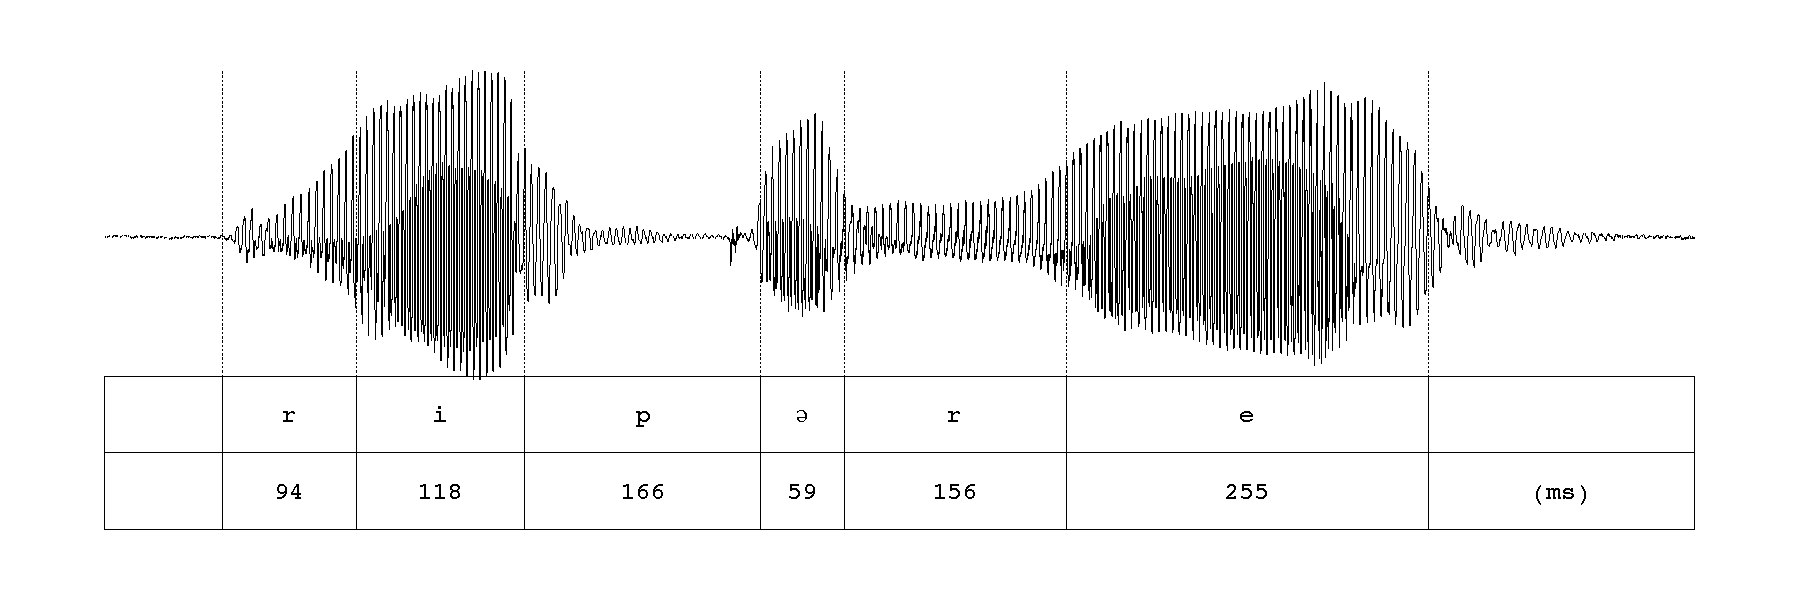
\includegraphics[width=\textwidth]{images/liverNOMSG-1403.pdf}}}
\resizebox{\columnwidth}{!}{%
\fbox{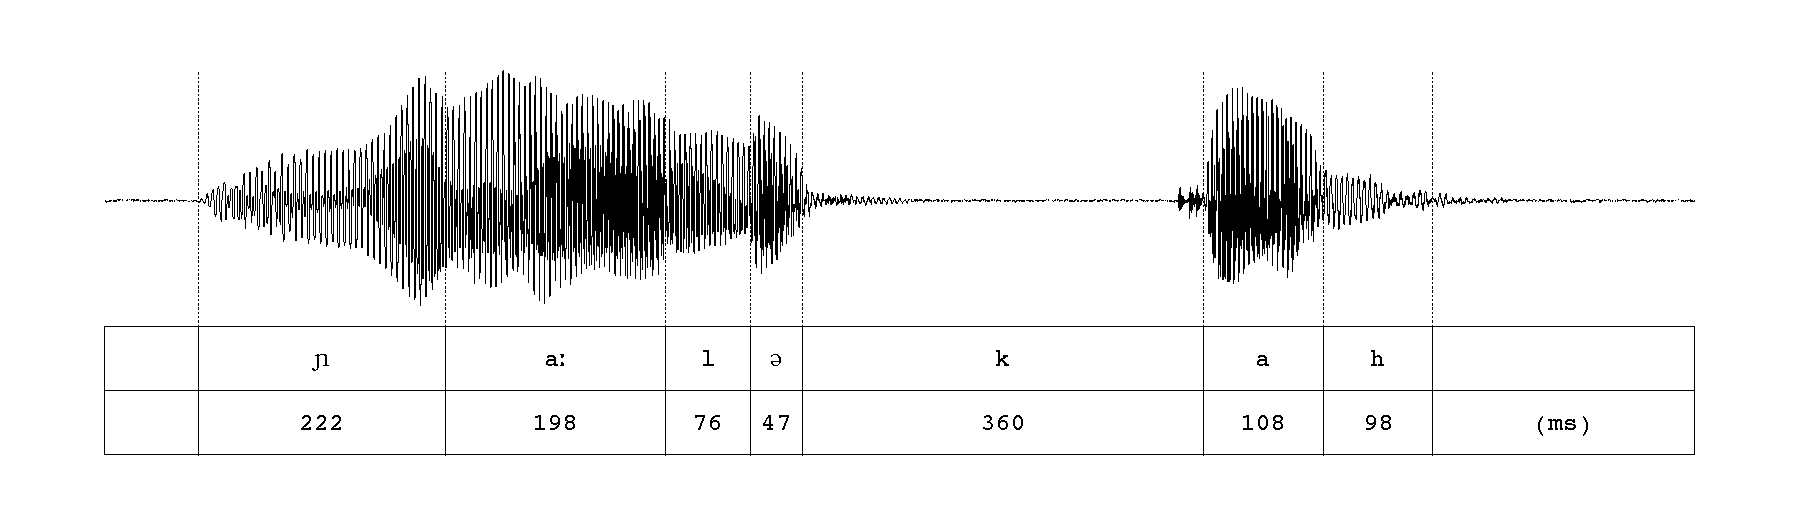
\includegraphics[width=\textwidth]{images/candyNOMSG-1277.pdf}}}
\caption[Waveforms of two words with an epenthetic schwa]{Waveforms of two words (\It{ribbre} ‘liver’ and \It{njálga} ‘candy’) with an epenthetic schwa, including segmental durations}\label{epentheticSchwaWaveforms}
\end{figure}


Speakers are rarely conscious of this vowel, and it is not reflected in the orthography. In neighboring Lule Saami, a similar epenthetic vowel exists and is predictable based on the prosodic and phonological structure of a word \citep[cf.][14-15]{Spiik1989}. It therefore seems likely that this epenthetic schwa is not phonemic in \PS\ either. However, more data is needed to confirm this and thoroughly describe its distribution. The fact that this epenthetic vowel seems to be significantly more prevalent in northern \PS\ dialects complicates the situation further. The examples in \REF{quick} through \REF{whitefishNOMSG} provide dialectal variants, with the more southern variant first (lacking the epenthetic vowel), and the more northern variant second (with the epenthetic schwa).
\ea\label{quick}
\Tn{\begin{tabular}{p{20mm} x{22mm} l}
\MR{2}{*}{/spaːjːta/} &[spaːjj̥ːta]\textasciitilde	& \It{spájta}	\\
				&[spaːj\Bf{ᵊ}ta] 			& ‘fast’ 		\\
\end{tabular}
\hfill\pbox{\textwidth}{\hfill\small[1711]\\\hfill\hyperlink{pit110518a}{\small[pit110518a.3m22s]}}}
\z
\ea\label{deliciousPRED}
\Tn{\begin{tabular}{p{20mm} x{21mm} l}
\MR{2}{*}{/ɲalːke/} 	&[ɲalːke]\textasciitilde	& \It{njallge}	\\
				&[ɲal\Bf{ᵊ}kːe] 			& ‘tasty’ 		\\
\end{tabular}
\hfill\pbox{\textwidth}{\hfill\small[2323]\\\hfill\hyperlink{pit081111}{\small[pit081111.2m59s]}}}
\z
\ea\label{whitefishNOMSG}
\Tn{\begin{tabular}{p{20mm} x{23mm} l}
\MR{2}{*}{/ʧu͡avːʧa/}	&[ʧu͡aʋːʧa]\textasciitilde	& \It{tjuavvtja}				\\
				&\MR{2}{*}{[ʧu͡oʋ\Bf{ᵊ}ʧa]} 	& ‘whitefish\BS\Sc{nom.sg}’ 	\\
\end{tabular}
\hfill\pbox{.2\textwidth}{\hfill\small[1954]\\\hfill\hyperlink{pit0906_Ahkajavvre_a}{\small[pit0906\_Ahka-}\\\hbox{}\hfill\hyperlink{pit0906_Ahkajavvre_a}{\small javvre\_a.168]}}}
\z



%%%%%%% THIS IS NOT USED FOR THE ENTIRE COMPILATION, but only for individual chapters!!!!

\clearpage
\addcontentsline{toc}{chapter}{Bibliography}\label{Bibliography}
\bibliography{PiteGrammarBibSDL}%for bibtex
%\printbibliography%[title=Works Cited]%%for biber!






%%%NAME INDEX doesn’t work!?!? why???
\cleardoublepage\phantomsection%this allows hyperlink in ToC to work
\addcontentsline{toc}{chapter}{Name index}
\ohead{Name index}
\printindex[aut]

\cleardoublepage\phantomsection%this allows hyperlink in ToC to work
\addcontentsline{toc}{chapter}{Language index}
\ohead{Language index}
\printindex[lan]

\cleardoublepage\phantomsection%this allows hyperlink in ToC to work
\addcontentsline{toc}{chapter}{Subject index}
\ohead{Subject index}
\printindex


\end{document}
%\documentclass[ number=5
			   ,series=sidl
			   ,isbn=xxx-x-xxxxxx-xx-x
			   ,url=http://langsci-press.org/catalog/book/17
			   ,output=long   % long|short|inprep              
			   %,blackandwhite
			   %,smallfont
			   ,draftmode   
			  ]{LSP/langsci}                          

\usepackage{LSP/lsp-styles/lsp-gb4e}		% verhindert Komma bei mehrfachen Fußnoten?
                                                      
\usepackage{layout}
\usepackage{lipsum}

%%%% ABOVE FOR LangSciPress %%%%
%%%% ABOVE FOR LangSciPress %%%%
%%%% ABOVE FOR LangSciPress %%%%
\usepackage{libertine}%work-around solution for rendering problematic characters ʦ, ͡  (mostly in \textbf{})

\usepackage{longtable}%Double-lines (\hline\hline) aren’t typeset properly in ‘longtable’-environment across several pages! conflict with other package (maybe xcolor with option ‘tables’?)

\usepackage{multirow}

\usepackage{array} %allows, among other things, centering column content in a table while also specifying width, creates new column style "x" for center-alignment, "y" for right-alignment
\newcolumntype{x}[1]{>{\centering\hspace{0pt}}p{#1}}%
\newcolumntype{y}[1]{>{\raggedleft\hspace{0pt}}p{#1}}%

\usepackage[]{placeins}%using \FloatBarrier command, all floats still floating at that point will be typeset, and cannot cross that boundary. the option here \usepackage[section]{placeins} automatically adds \FloatBarrier to every \section command (only works for \section commands, nothing lower than that!)
%\usepackage{afterpage}%by using the command \afterpage{\clearpage}, all floats will appear, but no new page will be started, thus avoiding bad page breaks around floats

\usepackage{vowel} %for vowel space chart


%%%IS THIS NECESSARY??
%%%%following allows you to refer to footnotes (from http://anthony.liekens.net/index.php/LaTeX/MultipleFootnoteReferences)
%\newcommand{\footnoteremember}[2]{
%  \footnote{#2}
%  \newcounter{#1}
%  \setcounter{#1}{\value{footnote}}
%} \newcommand{\footnoterecall}[1]{
%  \footnotemark[\value{#1}]} 
%%%%previous allows you to refer to footnotes: use \footnoteremember{referenceText} in footnote, then \footnoterecall{referenceText} to refer.

\usepackage{tikz}%
\usetikzlibrary{plothandlers,matrix,decorations.text,shapes.arrows,shadows,chains,positioning,scopes}

\usepackage{synttree} %zeichnet linguistische Bäume
\branchheight{36pt}%sets height between rows in synttree

\usepackage{lscape}%used for landscape pages in index (list of recordings)

\usepackage{polyglossia}
\setmainlanguage{english}


%%%TAKE OUT FOR FINAL VERSION:
%%%TAKE OUT FOR FINAL VERSION:
%%%TAKE OUT FOR FINAL VERSION:

%%%%following readjusts margin text!
%\setlength{\marginparwidth}{20mm}
%\let\oldmarginpar\marginpar
%\renewcommand\marginpar[1]{\-\oldmarginpar[\raggedleft\footnotesize\vspace{-7pt}\color{red}\It{→ #1}]%
%{\raggedright\footnotesize\vspace{-7pt}\color{red}\It{→ #1}}}
%%%%previous readjusts margin text!

%%%The following lines set depth of ToC (LSP default is only 3 levels)!
%%%\renewcommand{\contentsname}{Table of Contents} % überschrift des inhaltsverzeichnisses
%\setcounter{secnumdepth}{5}%sets how deep section/subsection/subsubsections are numbered
%\setcounter{tocdepth}{5}%sets the depth of the ToC %but this doesn't seem to work!!!
%% new commands for LSP book (Grammar of Pite Saami, by J. Wilbur)

\newcommand{\PS}{Pite Saami}
\newcommand{\PSDP}{Pite Saami Documentation Project}
\newcommand{\WLP}{Wordlist Project}

\newcommand{\HANG}{\everypar{\hangindent15pt \hangafter1}}%also useful for table cells
\newcommand{\FB}{\FloatBarrier}%shortcut for this command to print all floats w/o pagebreak

\newcommand{\REF}[1]{(\ref{#1})}%adds parenthesis around the reference number, particularly useful for examples.%\Ref had clash with LSP!
\newcommand{\dline}{\hline\hline}%makes a double line in a table
\newcommand{\superS}[1]{\textsuperscript{#1}}%adds superscript element
\newcommand{\sub}[1]{$_{#1}$}%adds subscript element
\newcommand{\Sc}[1]{\textsc{#1}}%shortcut for small capitals (not to be confused with \sc, which changes the font from that point on)
\newcommand{\It}[1]{\textit{#1}}%shortcut for italics (not to be confused with \it, which changes the font from that point on)
\newcommand{\Bf}[1]{\textbf{#1}}%shortcut for bold (not to be confused with \bf, which changes the font from that point on)
\newcommand{\BfIt}[1]{\textbf{\textit{#1}}}
\newcommand{\BfSc}[1]{\textbf{\textsc{#1}}}
\newcommand{\Tn}[1]{\textnormal{#1}}%shortcut for normal text (undo italics, bolt, etc.)
\newcommand{\MC}{\multicolumn}%shortcut for multicolumn command in tabular environment - only replaces command, not variables!
\newcommand{\MR}{\multirow}%shortcut for multicolumn command in tabular environment - only replaces command, not variables!
\newcommand{\TILDE}{∼}%U+223C %OLD:~}%shortcut for tilde%command ‘\Tilde’ clashes with LSP!%
\newcommand{\BS}{\textbackslash}%backslash
\newcommand{\Red}[1]{{\color{red}{#1}}}%for red text
\newcommand{\Blue}[1]{{\color{blue}{#1}}}%for blue text
\newcommand{\PLUS}{+}%nicer looking plus symbol
\newcommand{\MINUS}{-}%nicer looking plus symbol
%    Was die Pfeile betrifft, kannst Du mal \Rightarrow \mapsto \textrightarrow probieren und dann \mathbf \boldsymbol oder \pbm dazutun.
\newcommand{\ARROW}{\textrightarrow}%→%dieser dicke Pfeil ➜ wird nicht von der LSP-Font unterstützt: %\newcommand{\ARROW}{{\fontspec{DejaVu Sans}➜}}
\newcommand{\DARROW}{\textleftrightarrow}%↔︎%DoubleARROW
\newcommand{\BULLET}{•}%
%%✓ does not exist in the default LSP font!
\newcommand{\CH}{\checkmark}%%\newcommand{\CH}{\fontspec{Arial Unicode MS}✓}%CH as in CHeck
%%following used to separate alternation forms for consonant gradation and umlaut patterns:
\newcommand{\Div}{‑}%↔︎⬌⟷⬄⟺⇔%non-breaking hyphen: ‑  
\newcommand{\QUES}{\textsuperscript{?}}%marks questionable/uncertain forms

\newcommand{\jvh}{\mbox{\It{j}-suffix} vowel harmony}%
%\newcommand{\Ptcl}{\Sc{ptcl} }%just shortcut for glossing ‘particle’
%\newcommand{\ATTR}{{\Sc{attributive}}}%shortcut for ATTRIBUTIVE in small caps
%\newcommand{\PRED}{{\Sc{predicative}}}%shortcut for PREDICATIVE in small caps
%\newcommand{\COMP}{{\Sc{comparative}}}%shortcut for COMPARATIVE in small caps
%\newcommand{\SUPERL}{{\Sc{superlative}}}%shortcut for SUPERLATIVE in small caps
\newcommand{\SG}{{\Sc{singular}}}%shortcut for SINGULAR in small caps
\newcommand{\DU}{{\Sc{dual}}}%shortcut for DUAL in small caps
\newcommand{\PL}{{\Sc{plural}}}%shortcut for PLURAL in small caps
%\newcommand{\NOM}{{\Sc{nominative}}}%shortcut for NOMINATIVE in small caps
%\newcommand{\ACC}{{\Sc{accusative}}}%shortcut for ACCUSATIVE in small caps
%\newcommand{\GEN}{{\Sc{genitive}}}%shortcut for GENITIVE in small caps
%\newcommand{\ILL}{{\Sc{illative}}}%shortcut for ILLATIVE in small caps
%\newcommand{\INESS}{{\Sc{inessive}}}%shortcut for INESSIVE in small caps
\newcommand{\ELAT}{{\Sc{elative}}}%shortcut for ELATIVE in small caps
%\newcommand{\COM}{{\Sc{comitative}}}%shortcut for COMITATIVE in small caps
%\newcommand{\ABESS}{{\Sc{abessive}}}%shortcut for ABESSIVE in small caps
%\newcommand{\ESS}{{\Sc{essive}}}%shortcut for ESSIVE in small caps
%\newcommand{\DIM}{{\Sc{diminutive}}}%shortcut for DIMINUTIVE in small caps
%\newcommand{\ORD}{{\Sc{ordinal}}}%shortcut for ORDINAL in small caps
%\newcommand{\CARD}{{\Sc{cardinal}}}%shortcut for CARDINAL in small caps
%\newcommand{\PROX}{{\Sc{proximal}}}%shortcut for PROXIMAL in small caps
%\newcommand{\DIST}{{\Sc{distal}}}%shortcut for DISTAL in small caps
%\newcommand{\RMT}{{\Sc{remote}}}%shortcut for REMOTE in small caps
%\newcommand{\REFL}{{\Sc{reflexive}}}%shortcut for REFLEXIVE in small caps
%\newcommand{\PRS}{{\Sc{present}}}%shortcut for PRESENT in small caps
%\newcommand{\PST}{{\Sc{past}}}%shortcut for PAST in small caps
%\newcommand{\IMP}{{\Sc{imperative}}}%shortcut for IMPERATIVE in small caps
%\newcommand{\POT}{{\Sc{potential}}}%shortcut for POTENTIAL in small caps
\newcommand{\PROG}{{\Sc{progressive}}}%shortcut for PROGRESSIVE in small caps
\newcommand{\PRF}{{\Sc{perfect}}}%shortcut for PERFECT in small caps
\newcommand{\INF}{{\Sc{infinitive}}}%shortcut for INFINITIVE in small caps
%\newcommand{\NEG}{{\Sc{negative}}}%shortcut for NEGATIVE in small caps
\newcommand{\CONNEG}{{\Sc{connegative}}}%shortcut for CONNEGATIVE in small caps
\newcommand{\ATTRs}{{\Sc{attr}}}%shortcut for ATTR in small caps
\newcommand{\PREDs}{{\Sc{pred}}}%shortcut for PRED in small caps
%\newcommand{\COMPs}{{\Sc{comp}}}%shortcut for COMP in small caps
%\newcommand{\SUPERLs}{{\Sc{superl}}}%shortcut for SUPERL in small caps
\newcommand{\SGs}{{\Sc{sg}}}%shortcut for SG in small caps
\newcommand{\DUs}{{\Sc{du}}}%shortcut for DU in small caps
\newcommand{\PLs}{{\Sc{pl}}}%shortcut for PL in small caps
\newcommand{\NOMs}{{\Sc{nom}}}%shortcut for NOM in small caps
\newcommand{\ACCs}{{\Sc{acc}}}%shortcut for ACC in small caps
\newcommand{\GENs}{{\Sc{gen}}}%shortcut for GEN in small caps
\newcommand{\ILLs}{{\Sc{ill}}}%shortcut for ILL in small caps
\newcommand{\INESSs}{{\Sc{iness}}}%shortcut for INESS in small caps
\newcommand{\ELATs}{{\Sc{elat}}}%shortcut for ELAT in small caps
\newcommand{\COMs}{{\Sc{com}}}%shortcut for COM in small caps
\newcommand{\ABESSs}{{\Sc{abess}}}%shortcut for ABESS in small caps
\newcommand{\ESSs}{{\Sc{ess}}}%shortcut for ESS in small caps
%\newcommand{\DIMs}{{\Sc{dim}}}%shortcut for DIM in small caps
%\newcommand{\ORDs}{{\Sc{ord}}}%shortcut for ORD in small caps
%\newcommand{\CARDs}{{\Sc{card}}}%shortcut for CARD in small caps
\newcommand{\PROXs}{{\Sc{prox}}}%shortcut for PROX in small caps
\newcommand{\DISTs}{{\Sc{dist}}}%shortcut for DIST in small caps
\newcommand{\RMTs}{{\Sc{rmt}}}%shortcut for RMT in small caps
\newcommand{\REFLs}{{\Sc{refl}}}%shortcut for REFL in small caps
\newcommand{\PRSs}{{\Sc{prs}}}%shortcut for PRS in small caps
\newcommand{\PSTs}{{\Sc{pst}}}%shortcut for PST in small caps
\newcommand{\IMPs}{{\Sc{imp}}}%shortcut for IMP in small caps
\newcommand{\POTs}{{\Sc{pot}}}%shortcut for POT in small caps
\newcommand{\PROGs}{{\Sc{prog}}}%shortcut for PROG in small caps
\newcommand{\PRFs}{{\Sc{prf}}}%shortcut for PRF in small caps
\newcommand{\INFs}{{\Sc{inf}}}%shortcut for INF in small caps
\newcommand{\NEGs}{{\Sc{neg}}}%shortcut for NEG in small caps
\newcommand{\CONNEGs}{{\Sc{conneg}}}%shortcut for CONNEG in small caps

\newcommand{\subNP}{{\footnotesize\sub{NP}}}%shortcut for NP (nominal phrase) in subscript
\newcommand{\subVC}{{\footnotesize\sub{VC}}}%shortcut for VC (verb complex) in subscript
\newcommand{\subAP}{{\footnotesize\sub{AP}}}%shortcut for NP (adjectival phrase) in subscript
\newcommand{\subAdvP}{{\footnotesize\sub{AdvP}}}%shortcut for AdvP (adverbial phrase) in subscript
\newcommand{\subPP}{{\footnotesize\sub{PP}}}%shortcut for NP (postpoistional phrase) in subscript

\newcommand{\ipa}[1]{{\fontspec{Linux Libertine}#1}}%specifying font for IPA characters

\newcommand{\SEC}{§}%standardize section symbol and spacing afterwards
%\newcommand{\SEC}{§\,}%

\newcommand{\Nth}{{\footnotesize(\It{n})}}%used in table of numerals in ADJ chapter

%%newcommands for tables in introductionSDL.tex:
\newcommand{\cliticExs}[3]{\Tn{\begin{tabular}{p{28mm} c p{28mm} p{35mm}}\It{#1}&\ARROW &\It{#2} & ‘#3’\\\end{tabular}}}%specifically for the two clitic examples
\newcommand{\Grapheme}[1]{\It{#1}}%formatting for graphemes in orthography tables
%%new command for the section on orthographic examples; syntax: #1=orthography, #2=phonology, #3=gloss
\newcommand{\SpellEx}[3]{\Tn{\begin{tabular}{p{70pt} p{70pt} l}\ipa{/#2/}&\It{#1}& ‘#3’ \\\end{tabular}}}%formatting for orthographic examples (intro-Chapter)


%%new transl tier in gb4e; syntax: #1=free translation (in single quotes), #2=additional comments, z.B. literal meaning:
\newcommand{\Transl}[2]{\trans\Tn{‘#1’ #2}}%new transl tier in gb4e;
\newcommand{\TranslMulti}[2]{\trans\hspace{12pt}\Tn{‘#1’ #2}}%new transl tier in gb4e for a dialog to be included under a single example number


%% used for examples in the Prosody and Segmental phonology chapters:
\newcommand{\PhonGloss}[7]{%PhonGloss = Phonology Gloss;
%pattern: \PhonGloss{label}{phonemic}{phonetic}{orthographic}{gloss}{recording}{utterance}
\ea\label{#1}
\Tn{\begin{tabular}[t]{p{30mm} l}
\ipa{/#2/}	& \It{#4} \\
\ipa{[#3]}	&\HANG ‘#5’\\%no table row can start with square brackets! thus the workaround with \MC
\end{tabular}\hfill\hyperlink{#6}{{\small\textnormal[pit#6#7]}}%\index{Z\Red{rec}!\Red{pit#6}}\index{Z\Red{utt}!\Red{pit#6#7} \Blue{Phon}}
}
\z}
\newcommand{\PhonGlossWL}[6]{%PhonGloss = Phonology Gloss for words from WORDLIST, not from corpus!;
%pattern: \PhonGloss{label}{phonemic}{phonetic}{orthographic}{gloss}{wordListNumber}
\ea\label{#1}
\Tn{\begin{tabular}[t]{p{30mm} l}
\ipa{/#2/}	& \It{#4} \\
\ipa{[#3]}	&\HANG ‘#5’\\%no table row can start with square brackets! thus the workaround with \MC
\end{tabular}\hfill\hyperlink{explExs}{{\small\textnormal[#6]}}%\index{Z\Red{wl}!\Red{#6}\Blue{Phon}}
}
\z}

%%for derivation examples in the derivational morphology chapter!
%syntax: \DerivExam{#1}{#2}{#3}{#4}{#5}{#6}
%#1: base, #2: base-gloss, #3: derived form, #4: derived form gloss, #5: derived form translation, #6: pit-recording, #7: utterance number
\newcommand{\DW}{28mm}%for following three commands, to align arrows throughout
%%%%OLD:
%%%\newcommand{\DerivExam}[7]{\Tn{\begin{tabular}[t]{p{\DW}cl}\It{#1}&\ARROW&\It{#3}\\#2&&#4\\\end{tabular}\hfill\pbox{.3\textwidth}{\hfill‘#5’\\\hbox{}\hfill\hyperlink{pit#6}{{\small\textnormal[pit#6.#7]}}}
%%%%\index{Z\Red{rec}!\Red{pit#6}}\index{Z\Red{utt}!\Red{pit#6.#7}}
%%%}}
%NEW:
\newcommand{\DerivExam}[7]{\Tn{
\begin{tabular}[t]{p{\DW}x{5mm}l}\It{#1}&\ARROW&\It{#3}\\\end{tabular}\hfill‘#5’\\
\hspace{1mm}\begin{tabular}[t]{p{\DW}x{5mm}l}#2&&#4\\\end{tabular}\hfill\hyperlink{pit#6}{{\small\textnormal[pit#6.#7]}}
%\index{Z\Red{rec}!\Red{pit#6}}\index{Z\Red{utt}!\Red{pit#6.#7}}
}}
%%same as above, but supress any reference to a specific utterance
\newcommand{\DerivExamX}[7]{\Tn{
\begin{tabular}[t]{p{\DW}x{5mm}l}\It{#1}&\ARROW&\It{#3}\\\end{tabular}\hfill‘#5’\\
\hspace{1mm}\begin{tabular}[t]{p{\DW}x{5mm}l}#2&&#4\\\end{tabular}\hfill\hyperlink{pit#6}{{\small\textnormal[pit#6]\It{e}}}
%\index{Z\Red{rec}!\Red{pit#6}}\index{Z\Red{utt}!\Red{pit#6.#7}}
}}
\newcommand{\DerivExamWL}[6]{\Tn{
\begin{tabular}[t]{p{\DW}x{5mm}l}\It{#1}&\ARROW&\It{#3}\\\end{tabular}\hfill‘#5’\\
\hspace{1mm}\begin{tabular}[t]{p{\DW}x{5mm}l}#2&&#4\\\end{tabular}\hfill\hyperlink{explExs}{{\small\textnormal[#6]}}
%\index{Z\Red{wl}!\Red{#6}}
}}


%formatting of corpus source information (after \transl in gb4e-environments):
\newcommand{\Corpus}[2]{\hspace*{1pt}\hfill{\small\mbox{\hyperlink{pit#1}{\Tn{[pit#1.#2]}}}}%\index{Z\Red{rec}!\Red{pit#1}}\index{Z\Red{utt}!\Red{pit#1.#2}}
}%
\newcommand{\CorpusE}[2]{\hspace*{1pt}\hfill{\small\mbox{\hyperlink{pit#1}{\Tn{[pit#1.#2]}}\It{e}}}%\index{Z\Red{rec}!\Red{pit#1}}\index{Z\Red{utt}!\Red{pit#1.#2}\Blue{-E}}
}%
%%as above, but necessary for recording names which include an underline because the first variable in \href understands _ but the second variable requires \_
\newcommand{\CorpusLink}[3]{\hspace*{1pt}\hfill{\small\mbox{\hyperlink{pit#1}{\Tn{[pit#2.#3]}}}}%\index{Z\Red{rec}!\Red{pit#2}}\index{Z\Red{utt}!\Red{pit#2.#3}}
}%
%%as above, but for newer recordings which begin with sje20 instead of pit
\newcommand{\CorpusSJE}[2]{\hspace*{1pt}\hfill{\small\mbox{\hyperlink{sje20#1}{\Tn{[sje20#1.#2]}}}}%\index{Z\Red{rec}!\Red{sje20#1}}\index{Z\Red{utt}!\Red{sje20#1.#2}}
}%
\newcommand{\CorpusSJEE}[2]{\hspace*{1pt}\hfill{\small\mbox{\hyperlink{sje20#1}{\Tn{[sje20#1.#2]}}\It{e}}}%\index{Z\Red{rec}!\Red{sje20#1}}\index{Z\Red{utt}!\Red{sje20#1.#2}\Blue{-E}}
}%











%%hyphenation points for line breaks
%%add to TeX file before \begin{document} with:
%%%%hyphenation points for line breaks
%%add to TeX file before \begin{document} with:
%%\include{hyphenationSDL}
\hyphenation{
ab-es-sive
affri-ca-te
affri-ca-tes
Ahka-javv-re
al-ve-o-lar
com-ple-ments
%check this:
de-cad-es
fri-ca-tive
fri-ca-tives
gemi-nate
gemi-nates
gra-pheme
gra-phemes
ho-mo-pho-nous
ho-mor-ga-nic
mor-pho-syn-tac-tic
or-tho-gra-phic
pho-neme
pho-ne-mes
phra-ses
post-po-si-tion
post-po-si-tion-al
pre-as-pi-ra-te
pre-as-pi-ra-ted
pre-as-pi-ra-tion
seg-ment
un-voiced
wor-king-ver-sion
}
\hyphenation{
ab-es-sive
affri-ca-te
affri-ca-tes
Ahka-javv-re
al-ve-o-lar
com-ple-ments
%check this:
de-cad-es
fri-ca-tive
fri-ca-tives
gemi-nate
gemi-nates
gra-pheme
gra-phemes
ho-mo-pho-nous
ho-mor-ga-nic
mor-pho-syn-tac-tic
or-tho-gra-phic
pho-neme
pho-ne-mes
phra-ses
post-po-si-tion
post-po-si-tion-al
pre-as-pi-ra-te
pre-as-pi-ra-ted
pre-as-pi-ra-tion
seg-ment
un-voiced
wor-king-ver-sion
}\begin{document}\tableofcontents\clearpage

%%%%%%%%%%%%%%%%%%%%%%%%%%%%%%%%% ALL THE ABOVE TO BE COMMENTED OUT FOR COMPLETE DOCUMENT! %%%%%%%%%%%


%%%%%%%%%%%%%%%%%%%%%%%%%%%%%% C H A P T E R %%%%%%%%%%%%%%%%%%%%%%%%%%%%%
%%%%%%%%%%%%%%%%%%%%%%%%%%%%%% C H A P T E R %%%%%%%%%%%%%%%%%%%%%%%%%%%%%
\chapter{Morphological patterns and word classes}\label{morphWordClassCh}
Morphology plays an essential role in \PS, a highly synthetic language. Based on morphological patterning and in addition to syntactic criteria, seven word classes can be posited. \SEC\ref{morphology} first provides an introduction to morphological phenomena in \PS, before \SEC\ref{introWordForms} summarizes the word classes.  


\section{Overview of morphology}\label{morphology}
A number of inflectional categories exist in \PS; Table \vref{summaryMorphCats} provides a summary of inflectional categories relevant for each word class or sub-category. 
Derivational morphology is commonly used to create nouns, verbs, and, to a lesser extent, adjectives and adverbs. %\footnote{\Red{Historically, at least attributive adjectives were probably derived as well, but synchronically, this is no longer the case; cf. \SEC\ref{notePredNounsAdjs}.}} 
Both derivational\is{derivation} and inflectional\is{inflection} morphology manifest themselves linearly (by suffixing) or non-linearly, via consonant gradation, umlaut and/or vowel harmony. More often than not, linear and non-linear morphological phenomena are combined. 
\begin{table}[h]\centering
\caption{Inflectional categories for pertinent word classes and sub-categories of word classes}\label{summaryMorphCats}
\begin{tabular}{ll}\mytoprule
{word class/sub-category}	&{inflectional categories}	\\\hline
{verbs}	&	\\%\hline
\BULLET\ finite forms	&person, tense, mood	\\%\hline
\BULLET\ non-finite forms	&aspect, connegation, etc.	\\%\hline
{nominals}	&	\\%\hline
\BULLET\ nouns			&case, number	\\%\hline
\BULLET\ interrogative, relative pronouns	&case, number	\\%\hline
\BULLET\ personal, reflexive pronouns			&case, number, person	\\%\hline
\BULLET\ demonstrative pronouns	&case, number, distance	\\%\hline
{adjectivals}	&	\\%\hline
\BULLET\ attributive adjectives			&comparative, superlative	\\%\hline
\BULLET\ predicative adjectives		&comparative, superlative, number	\\\mybottomrule
\end{tabular}
\end{table}

The present section only provides an overview of these various morphological phenomena, and is divided into \SEC\ref{linearMorphology} on linear morphology and \SEC\ref{morphophonology} on non-linear morphological processes. %(consonant gradation, umlaut and morphologically-triggered vowel harmony).
Because morphological behavior varies between the word classes, it is described in more detail individually in the relevant word class chapters.  

\FB

\subsection{Linear morphology}\label{linearMorphology}\is{morphology!linear|(}
Concerning linearly separable morphology, \PS\ is an exclusively suffixing language. Both inflectional and derivational suffixes exist. %, and can be ascertained on nouns, pronouns, adjectives, adverbs, verbs. 
The general linear morphological structure of \PS\ words has derivational suffixes attaching to a root before inflectional suffixes occur on the resulting stem, as illustrated by %\marginpar{make sure Figure \ref{linearMorphStructure} and Table \ref{summaryMorphCats} aren’t directly above one another}
Figure \vref{linearMorphStructure}.
\begin{figure}[h]\centering
[lexical root \PLUS\ derivational morphemes \PLUS\ inflectional morphemes]\sub{word}
\caption{General structure of linear morphology composing \PS\ words}\label{linearMorphStructure}
\end{figure}
\is{morphology!linear|)}
%\subsection{Suffixes}\label{suffixes}
%\subsubsection{inflectional}\label{inflectionalSuffixes}
%\subsubsection{derivational}\label{derivationalSuffixes}
%


\subsection{Non-linear morphology (morphophonology)}\label{morphophonology}\is{morphology!non-linear|(}
There are three ways %\marginpar{mention stem extension for verb morphology?} %eigentlich ja.
in which non-linear morphology can be expressed in \PS:
\begin{itemize}
\item{stem consonant alternations (consonant gradation)}
\item{stem vowel alternations in V1 position (umlaut)}
\item{regressive vowel harmony in V1 and V2 vowels}
\end{itemize}
These are triggered by a word’s position %paradigmatic relationship 
within an inflectional paradigm, or in derivation. All inflectional non-linear morphology is restricted to the final foot\is{foot} of a given word, while derivational non-linear morphology can also occur in a non-ultimate foot. Non-linear processes may apply simultaneously. The following sections describe these phenomena in more detail: \SEC\ref{Cgrad} for consonant gradation, \SEC\ref{umlaut} for umlaut and \SEC\ref{VH} for vowel harmony.\footnote{Cf. \citet{KorhonenM1969} for historical explanations of these morphophonological processes in Saami.} 


\subsubsection{Consonant gradation}\label{Cgrad}\is{consonant gradation|(}
The term \It{consonant gradation}\footnote{This term is quite common in Saami linguistics, e.g.,~in \citet{Feist2010}, although it is also known as ‘grade alternation’, e.g.,~in \citet{Sammallahti1998}. As much of the literature on Saami linguistics is in languages other than English, it may be useful to provide some translations of the term ‘consonant gradation’: German: \It{Stufenwechsel}, Swedish: \It{stadieväxling}, Finnish: \It{astevaihtelu}, Hungarian: \It{fokváltakozás} and Russian: \It{чередование ступеней}.} 
refers to regular alternations of the consonant phonemes in the consonant center of the final foot of a word.\footnote{Cf. \SEC\ref{prosodicDomains} on prosodic positions, including the foot and the consonant center.} 
%Many, but not all, lexical items are subject to consonant gradation. 

All consonant phonemes in the consonant center are included in the present classification of such alternations.
These alternations come in pairs of stem allomorphs that differ quantitatively and/or qualitatively. 
Alternations can be between a preaspirated\is{aspiration!preaspiration} and the corresponding non-aspirated consonant \mbox{(ʰx\Div x)},  
 a geminate\is{geminate} consonant and the corresponding singleton consonant \mbox{(xː\Div x)}, 
 a geminate\PLUS singleton and the corresponding singleton\PLUS singleton \mbox{(xːy\Div xy)}, 
 two singletons and only the latter singleton \mbox{(xy\Div y)}, 
and  three singletons and only the initial and final singleton \mbox{(xyz\Div xz)}.\footnote{There are certainly other ways to classify these alternations in the consonant center as well. For instance, one could disregard any consonant phonemes that are present in both alternations (then \mbox{xː\Div x} and \mbox{xːy\Div xy} would be the same type), or consider the xː\Div x and ʰxː\Div x patterns in Table \ref{CgradPatternSummary} to be the same type as simply a case of alternating consonant phonemes. However, the patterns in the present classification demonstrate the regularity of patterning between phonological features (such as geminate vs. singleton).}  

These patterns and the attested alternations are provided in Table \vref{CgradPatternSummary}. 
\begin{table}[h]\centering
\caption{Consonant center gradation patterns}\label{CgradPatternSummary}
\begin{tabular}{c c c p{240pt}}\mytoprule
%\MC{3}{c}{{pattern}}&\\
strong&\DARROW &weak	&{attested alternations}\\\hline
%\MC{4}{l}{\It{qualitative differences}}\\
ʰx	&\DARROW &x		
	& ʰp\Div p, ʰt\Div t, ʰk\Div k, ʰʦ\Div ʦ, ʰʧ\Div ʧ \\
%\MC{4}{l}{\It{quantitative differences}}\\
%\MC{4}{l}{geminate\Div singleton}\\
xː	&\DARROW &x
	& fː\Div f, vː\Div v, sː\Div s, ʃː\Div ʃ, mː\Div m, nː\Div n, ɲː\Div ɲ, rː\Div r, lː\Div l, jː\Div j \\
&&%ʰxː	&\Div &ʰx
	& ʰpː\Div ʰp, ʰtː\Div ʰt, ʰkː\Div ʰk, ʰʧː\Div ʰʧ, ʰʦː\Div ʰʦ \\
%	& !pː\Div p, ʰpː\Div ʰp, !tː\Div t, ʰtː\Div ʰt, !kː\Div k, ʰkː\Div ʰk, !ʧː\Div ʧ, ʰʧː\Div ʰʧ, !ʦː\Div ʦ, ʰʦː\Div ʰʦ, fː\Div f, vː\Div v, sː\Div s, ʃː\Div ʃ, mː\Div m, nː\Div n, ɲː\Div ɲ, rː\Div r, lː\Div l, jː\Div j \\
%\MC{4}{l}{preaspirated singleton\Div singleton}\\
%\MC{4}{l}{geminate+singleton\Div singleton+singleton}\\
xːy	&\DARROW & xy
	& pːt\Div pt, pːk\Div pk, pːʦ\Div pʦ, pːʧ\Div pʧ, pːs\Div ps, pːm\Div pm, pːn\Div pn, pːɲ\Div pɲ, pːr\Div pr, pːl\Div pl, pːj\Div pj, tːk\Div tk, tːm\Div tm, tːn\Div tn, tːɲ\Div tɲ, kːt\Div kt, kːʧ\Div kʧ, kːʦ\Div kʦ, kːs\Div ks, kːʃ\Div kʃ, kːŋ\Div kŋ, kːl\Div kl, \\
	&&& fːt\Div ft, fːn\Div n, vːt\Div vt, vːk\Div vk, vːʦ\Div vʦ, vːʧ\Div vʧ, vːs\Div vs, vːʃ\Div vʃ, vːr\Div vr, vːl\Div vl, vːj\Div vj, sːp\Div sp, sːt\Div st, sːk\Div sk, sːm\Div sm, sːn\Div sn, ʃːk\Div ʃk, \\
	&&& mːs\Div ms, mːʃ\Div mʃ, nːt\Div nt, ŋːk\Div ŋk \\%, mːʰp\Div mʰp, mːʰk\Div mʰk, nːʰt\Div nʰt, nːʰʦ\Div nʰʦ, ŋːʰk\Div ŋʰk, \\
	&&&rːp\Div rp, rːt\Div rt, rːk\Div rk, rːʦ\Div rʦ, rːf\Div rf, rːs\Div rs, rːʃ\Div rʃ, rːf\Div rf, rːv\Div rv, rːj\Div rj, lːp\Div lp, lːt\Div lt, lːk\Div lk, lːf\Div lf, lːv\Div lv, lːs\Div ls, lːj\Div lj, jːp\Div jp, jːt\Div jt, jːk\Div jk, jːs\Div js, jːf\Div jf, jːv\Div jv, jːr\Div jr, jːl\Div jl \\%, rːʰp\Div rʰp, rːʰt\Div rʰt, rːʰk\Div rʰk, rːʰʧ\Div rʰʧ, rːʰʦ\Div rʰʦ, lːʰp\Div lʰp, lːʰt\Div lʰt, lːʰk\Div lʰk, lːʰʦ\Div lʰʦ, lːʰʧ\Div lʰʧ, jːʰt\Div jʰt, jːʰk\Div jʰk, jːʰʧ\Div jʰʧ, jːʰʦ\Div jʰʦ\\%
%\MC{4}{l}{geminate+preaspirated singleton\Div preaspirated singleton+singleton}\\
&&%xːʰy	&\Div & xʰy	
	& mːʰp\Div mʰp, mːʰk\Div mʰk, nːʰt\Div nʰt, nːʰʦ\Div nʰʦ, ŋːʰk\Div ŋʰk, \\
	&&&rːʰp\Div rʰp, rːʰt\Div rʰt, rːʰk\Div rʰk, rːʰʧ\Div rʰʧ, rːʰʦ\Div rʰʦ, lːʰp\Div lʰp, lːʰt\Div lʰt, lːʰk\Div lʰk, lːʰʦ\Div lʰʦ, lːʰʧ\Div lʰʧ, jːʰt\Div jʰt, jːʰk\Div jʰk, jːʰʧ\Div jʰʧ, jːʰʦ\Div jʰʦ \\%
%xy	&\Div &x		&  \\%ʰpp-ʰp (assumes that there is no geminate ʰpː but instead ʰp+p)%ADAPTED ANALYSISː ʰpː-ʰp
%\MC{4}{l}{singleton12\Div singleton2}\\
xy	&\DARROW &y		
	& pm\Div m, pɲ\Div ɲ, tn\Div n, tɲ\Div ɲ, tj\Div j, kŋ\Div ŋ \\
%\MC{4}{l}{singleton123\Div singleton13}\\
xyz	&\DARROW & xz	
	& vtn\Div vn, vtɲ\Div vɲ, rpm\Div rm, rtn\Div rn, rtj\Div rj, lpm\Div lm, ltn\Div ln, ltɲ\Div lɲ, jpm\Div jm, jtn\Div jn \\\mybottomrule
\end{tabular}
\end{table}
The term \It{strong grade}\is{consonant gradation!strong grade} (abbreviated ‘str’) is used to refer to the form with preaspiration\is{aspiration!preaspiration}, a geminate\is{geminate} or more consonant segments than the corresponding form. Likewise, the term \It{weak grade}\is{consonant gradation!weak grade} (abbreviated ‘wk’) refers to the form lacking a preaspirated or geminate consonant, or having fewer consonant segments, respectively. 
To facilitate reading Table \ref{CgradPatternSummary}, the attested alternations for each pattern are organized by alternations with a non-aspirated element first, followed by patterns with at least one preaspirated element. Furthermore, the individual lists of alternations are organized by mode of articulation and by the order set forth in the consonant phoneme inventory in Table \vref{Cphonemes}. 
Some examples illustrating this can be found below. 


The minimal pair in \REF{CgradEx3} shows a consonant gradation alternation \mbox{/ʰp\Div p/}, which corresponds to the pattern \mbox{ʰx\Div x}. %in Table \ref{CgradPatternSummary}. 
\ea\label{CgradEx3}%várre mountain\BS\Sc{nom.sg} / váre mountain\BS\Sc{nom.pl} 
\Tn{\begin{tabular}{c c}
/dɔ{ʰp}e/		&/dɔ{p}e/\\
\It{dåhpe}		&\It{dåbe}\\
house\BS\Sc{nom.sg}	&house\BS\Sc{gen.sg}	\\
\end{tabular}
\hfill\hyperlink{pit100324}{{\small [pit100324]}}}
\z

The minimal pairs in \REF{CgradEx1a} and \REF{CgradEx1b} are examples of consonant gradation patterns which differ in a geminate\Div singleton alternation. The consonant gradation alternations illustrated are \mbox{/vː\Div v/} and \mbox{/rːk\Div rk/}, respectively, and correspond to the patterns \mbox{xː\Div x} and \mbox{xːy\Div xy}. % in Table \ref{CgradPatternSummary}. 
%In the first example, a geminate /vː/ in the consonant center of the \Sc{3sg.prs} form alternates with a singleton /v/ in the \Sc{2sg.prs} form. In the latter example, geminate\PLUS singleton /rːk/ in \Sc{nom.sg} alternates with two singeltons /rk/ in \Sc{nom.pl}. 
\ea\label{CgradEx1a}%várre mountain\BS\Sc{nom.sg} / váre mountain\BS\Sc{nom.pl} 
\Tn{\begin{tabular}{c c}
/saː{vː}a/		&/saː{v}a/\\
\It{sávva}		&\It{sáva}\\
wish\BS\Sc{3sg.prs}	&wish\BS\Sc{2sg.prs}\\
\end{tabular}
\hfill\hyperlink{pit100323a}{{\small [pit100323a]}}}
\z
\ea\label{CgradEx1b}%várre mountain\BS\Sc{nom.sg} / váre mountain\BS\Sc{nom.pl} 
\Tn{\begin{tabular}{c c}
/pɛ{rːk}o/	&/pe{rk}o/\\
\It{bärrgo}		&\It{biergo}\\
meat\BS\Sc{nom.sg}	&meat\BS\Sc{nom.pl}\\
\end{tabular}
\hfill\hyperlink{pit090926}{{\small [pit090926]}}}
\z

The minimal pairs in \REF{CgradEx2a} and \REF{CgradEx2b} are examples of consonant gradation patterns in which a phoneme present in the first form is absent in the second form. The consonant gradation alternations illustrated here are \mbox{/tn\Div n/} and \mbox{/jpm\Div jm/}, respectively, and correspond to the patterns \mbox{xy\Div y} and \mbox{xyz\Div xz}. %in Table \ref{CgradPatternSummary}. 
%Finally, the minimal pair in \REF{CgradEx3} is an example of a consonant gradation pattern that alternates in both quantity and quality, as it alternates between a consonant center consisting of the three segments /jpm/ in the \Sc{nom.sg} form, and a consonant center consisting of the two segments /jm/ in the \Sc{nom.pl} form. 
%, as it alternates between the segment /ʰp/ in the consonant center of the \Sc{nom.sg} form, and the segment /p/ in the \Sc{gen.sg} form.
\ea\label{CgradEx2a}%várre mountain\BS\Sc{nom.sg} / váre mountain\BS\Sc{nom.pl} 
\Tn{\begin{tabular}{c c}
/a{tn}a/		&/a{n}a/\\
\It{adna}		&\It{ana}\\
have\BS\Sc{3sg.prs}	&have\BS\Sc{2sg.prs}	\\
\end{tabular}
\hfill\hyperlink{pit101208}{{\small [pit101208]}}}
\z
\ea\label{CgradEx2b}%várre mountain\BS\Sc{nom.sg} / váre mountain\BS\Sc{nom.pl} 
\Tn{\begin{tabular}{c c}
/vaː{jpm}o/		&/vaː{jm}o/\\
\It{vájbmo}		&\It{vájmo}\\
heart\BS\Sc{nom.sg}	&heart\BS\Sc{nom.pl}	\\
\end{tabular}
\hfill\hyperlink{pit110413a}{{\small [pit110413a]}}}
\z

As may be inferred from the examples above, paradigmatic alternations between \mbox{\Sc{nom.sg}} and \mbox{\Sc{nom.pl}} forms for nouns, or between \Sc{2sg.prs} and \Sc{3sg.prs} forms for verbs are often a good source of minimal pairs concerning consonant gradation alternations, and are a useful way to determine consonant gradation patterns. 

Note that the geminate\is{geminate} plosives\is{plosive} and affricates\is{affricate} \mbox{/pː\,tː\,kː\,ʦː\,ʧː/} are lacking in Table \vref{CgradPatternSummary} for the pattern \mbox{xː\Div x}, although alternations such as \mbox{pː\Div p} could be expected. However, due to a lack of sufficient data and some conflicting data in the corpus, it is not entirely clear what the current status is for consonant gradation in words with a consonant center consisting solely of a geminate plosive or affricate. The fact that \PS\ lacks consonant gradation in a limited number of contexts is one of the main differences to Lule Saami to the north, which does not lack consonant gradation, and Ume Saami to the south, which features consonant gradation even less frequently \citep[cf.][21-23]{Sammallahti1998}. 
The example in \REF{CgradEx4a} illustrates a word clearly lacking consonant gradation in the corpus data, here with the geminate velar plosive /kː/. 
\ea\label{CgradEx4a}%
\Tn{\begin{tabular}{c c c}
/vaː{kː}e/	&/vaː{kː}e/	&(*/vaː{k}e/)\\
\It{vágge}		&\It{vágge}&\\
valley\BS\Sc{nom.sg}	& valley\BS\Sc{nom.pl}	&	\\%
\end{tabular}
\hfill\hyperlink{pit110522}{{\small [pit110522]}}}
\z

Corpus data also indicate that variation within the \PS\ area complicates things. For instance, the adjective \It{tjábbe} ‘beautiful’ undergoes consonant gradation in the speech\is{dialect variation} of speakers from the northern parts of Arjeplog, but does not for southern speakers, as illustrated in \REF{CgradEx4b}. For northern speakers, the gradation is realized as an alternation in voicing, and not length. 
\ea\label{CgradEx4b}%
\Tn{\begin{tabular}{c c c}
			&southern	&northern	\\
/ʧaː{pː}a/	&/ʧaː{pː}e/	&/ʧaː{bː}e/\\
\It{tjábba}		&\MC{2}{c}{\It{tjábbe}}\\
beautiful\BS\Sc{attr}	&\MC{2}{c}{beautiful\BS\Sc{pred}}\\
\end{tabular}
\hfill\hyperlink{pit110522}{{\small [pit110522}}, \hyperlink{sje20131017}{{\small sje20131017]}
}}
\z
This being the case, some speakers from farther north may have further voiced plosive phonemes \mbox{/bː dː gː/} that only occur in consonant gradation alternations with the corresponding unvoiced phonemes \mbox{/pː tː kː/}. However, it is not clear based on the corpus data how widespread this feature is, or if it also affects geminate affricates. 

Finally, it is not clear from the corpus data what the status of the phonological contexts lacking consonant gradation mentioned in \citet[21]{Sammallahti1998} (working from a historical perspective and with older data) is. Further research is needed to complete the picture, and %, although due to the current state of the \PS\ language \citep[cf.][]{ValijarviWilbur2011}, gathering such data is becoming more and more difficult; 
variation within \PS\ and possible effects of language attrition should also be taken into consideration.\is{consonant gradation|)}



\subsubsection{Umlaut}\label{umlaut}\is{umlaut|(}
The term \It{umlaut} refers to regular allomorphic alternations of the vowels in the V1 position of a stem.\footnote{Cf. \SEC\ref{prosodicDomains} on prosodic positions, including V1 position.} 
The two umlaut patterns attested in the corpus are listed in Table \vref{umlautPatternSummary}. %\footnote{Due to the orthography being more phonetic than phonemic, particularly concerning umlaut, phonemic representations in IPA are used in Table \vref{umlautPatternSummary}. However, these umlaut alternations are typically represented orthographically by the graphemes \It{ä}\TILDE\It{ie} and \It{ua}\TILDE\It{uo}, respectively. Cf. \SEC\ref{orthography} on the orthographic representation of \PS.} %Generally speaking, in V1 position, /u͡a/ is spelled \It{u͡a}, and its allophone [uɛ] is spelled \It{uä}, while /o/ is spelled \It{uo}, but /e/ is spelled \It{e} or \It{ie}.} 
%Some examples to help illustrate this can be found below. 
\begin{table}[h]\centering
\caption{The two attested umlaut patterns}\label{umlautPatternSummary}
\begin{tabular}{ccccccc}\mytoprule
\MC{3}{c}{{IPA}}&	&\MC{3}{c}{{orthography}}\\\hline
ɛ &\DARROW& e &&\It{ä} &\DARROW& \It{ie} \\
u͡a &\DARROW& o &&\It{ua}/\It{uä} &\DARROW& \It{uo} \\\mybottomrule\end{tabular}
%\newcommand{\wz}{28pt}%only for spacing in the following table
%\begin{tabular}{|ccc|ccc|}\hline
%\MC{3}{|c}{\It{IPA}}&\MC{3}{|c|}{\It{orthographic}}\\\mybottomrule
%ɛ &\ARROW& e	&ä &\ARROW& ie\\
%u͡a &\ARROW& o	&ua/uä &\ARROW& uo	\\\hline
%\begin{tabular}{rx{\wz}p{12pt}x{\wz}x{\wz}p{12pt}x{\wz}p{30pt}}%\cline{2-7}
%		&\MC{6}{c}{\It{pattern}}&\\
%		&\MC{3}{c}{\It{A}}		&\MC{3}{c}{\It{B}}	&\\\cline{2-7}
%\It{phonemic}	&	ɛ &\MR{2}{*}{\DARROW}& e	& u͡a &\MR{2}{*}{\DARROW}& o	&\\%\cline{2-7}
%\It{orthographic}&	ä &			& ie	& ua/uä && uo &\\\cline{2-7}
%\end{tabular}
%\begin{tabular}{|c| ccc |}\hline
%A	&ɛ&:&e\\\hline
%B	&u͡a&:&o	\\\hline
%%C-grad&str&:&wk\\\hline
%\end{tabular}
\end{table}

These umlaut alternations are qualitative and not quantitative. %The first one consists of a pair, and the second a triplet. 
These alternations are not triggered by the phonological environment, but instead morphologically. 
The allomorph /ɛ/ in the first pattern is found in the same paradigmatic slots for each inflectional class as /u͡a/\footnote{Note that /u͡a/ has an allomorph [u͡ɛ] triggered by purely phonological vowel harmony; cf. \SEC\ref{Vua}.} 
in the second pattern, just as the allomorphs /e/ and /o/ also correspond to the same paradigmatic slots. 
%Paradigm slots featuring Inflectional forms with /ɛ/ (in umlaut pattern A) correspond to inflectional forms with both /uɛ/ and /ua/ in umlaut pattern B, while forms with /e/ from pattern A and forms with /uo/ from pattern B always correspond across paradigms.
Word forms for \It{bägge} ‘wind’ in \REF{umlautEx1} and for \It{buälldet} ‘burn’ in \REF{umlautEx2} provide examples of the two umlaut patterns.
%In \REF{umlautEx1} an example of umlaut pattern A is given. It alternates between /ɛ/ in the V1 vowel of the \Sc{nom.sg} form, and /e/ in the \Sc{nom.pl} form.
\ea\label{umlautEx1}%
\Tn{\begin{tabular}{c c}
/b{ɛ}gːa/		&/b{e}gːa/\\
\It{bägga}		&\It{biegga}\\
wind\BS\Sc{nom.sg}	&wind\BS\Sc{nom.pl}\\
\end{tabular}
\hfill\hyperlink{pit080621}{{\small [pit080621]}}}
\z
%
%%, as it alternates between /u͡a/ in the V1 vowel of the \Sc{nom.sg} form, and /o/ in the \Sc{nom.pl} form. %Note that the example in \REF{umlautEx2} reflects a more southern \PS\ dialect, and that the more northern dialects usually have the allophone [u͡ɛ] \It{uä} here. %, although the exact relationship between the dialects must be left to future study. 
\ea\label{umlautEx2}%
\Tn{\begin{tabular}{c c}
/p{u͡a}lːta/		&/p{o}lta/\\
\It{buallda}		&\It{buolda}\\
ignite\BS\Sc{3sg.prs}	&ignite\BS\Sc{2sg.prs}\\
%/lu͡akːta/		&/lokta/\\
%\It{luakkta		&\It{luokta\\
%bay\BS\Sc{nom.sg}	&bay\BS\Sc{nom.pl}\\
%\begin{tabular}{c c c}
%/lu͡ɛkːta/		&/lu͡ak:taj/ &/lokːta/\\
%\It{luäkkta		&\It{luakkta-j	&\It{luokta\\
%bay\BS\Sc{nom.sg}	&bay-\Sc{ill.sg}&bay\BS\Sc{nom.pl}\\
\end{tabular}
\hfill\hyperlink{pit101208}{{\small [pit101208]}}}
\z
For lexemes subject to consonant gradation, forms featuring /ɛ/ or /u͡a/ are typically in the strong grade\is{consonant gradation!strong grade}, while forms with /e/ or /o/ are normally in the weak grade\is{consonant gradation!weak grade}; cf. the word forms in example \REF{umlautEx2}. \is{umlaut|)}


\subsubsection{Vowel harmony}\label{VH}\is{vowel harmony|(}
The term \It{vowel harmony} (abbrviated ‘VH’) here refers to non-adjacent regressive phonological assimilation\is{assimilation} concerning the place of articulation of the V1 vowel of a stem in the context of certain V2 vowels.\footnote{Cf. \SEC\ref{prosodicDomains} on prosodic positions, including V1 and V2 positions.} 
Specifically, mid-high or high front vowels in V2 position in specific paradigmatic slots trigger raising of the vowel in V1 position. Because the paradigmatic slots that trigger vowel harmony differ between word classes and inflectional classes, and do not apply across the board, vowel harmony is not a purely phonological process, but morphophonological. Furthermore, the results of harmony on the same underlying vowel are inconsistent, and may be due to a word’s membership is certain morphological classes concerning vowel harmony. However, future research must be conducted to come to a more thorough conclusion on this. 

Verbs\is{verb} and nouns\is{noun} can be subject to vowel harmony, but the assimilation patterns vary both between these word classes and within them. 
Table \vref{VHsummaryTable} summarizes the various patterns and the word classes that they are attested in based on the current corpus. 
It is possible that, as a result of more documentation and study, this table may need to be updated. 
\begin{table}[h]\centering
\caption{Vowel harmony assimilation patterns and the word classes these are found in}\label{VHsummaryTable}
\begin{tabular}{lclcc}\mytoprule
%\begin{tabular}{x{30pt}cx{30pt}cc}\mytoprule
\MC{3}{c}{{VH pattern}}	&{nouns}	&{verbs}		\\\hline	
%\It{ &&\It{VH		&\It{nouns	&\It{verbs	\\\mybottomrule	
%				&&&\It{nouns	&\It{verbs	\\\mybottomrule
ɛ/e&\ARROW&i			&\CH	&\CH	\\
u͡a/o&\ARROW&u		&\CH	&\CH	\\
aː&\ARROW&ɛ			&\CH	&\CH	\\
ɔ&\ARROW&u			&\CH	&\CH	\\
a&\ARROW&ɛ			&\CH	&	\\
a&\ARROW&i			&		&\CH	\\
aː&\ARROW&i			&		&\CH	\\
a&\ARROW&e			&		&\CH	\\\mybottomrule
\end{tabular}
\end{table}

The morphological categories that trigger vowel harmony also vary. This is the case not only between nouns and verbs (as these have different inflectional categories), but also between inflectional classes for verbs. These categories are presented in Table \vref{VHtriggerSummary}. %on page \pageref{VHtriggerSummary}. 
\begin{table}[h]\centering
\caption{Paradigm slots that trigger vowel harmony}\label{VHtriggerSummary}
\begin{tabular}{lll}\mytoprule
%\begin{tabular}{ccp{178pt}}\mytoprule
{word class}&{inflectional class}&{forms triggering VH}	\\\hline
nouns	&class Ie			&\Sc{gen.pl, acc.pl, ill.pl, iness.pl,}	\\%\hline
		&				&\Sc{elat.pl, com.sg, com.pl} \\%\hline
verbs	&class II			&\Sc{1du.prs, 3pl.prs, 1sg.pst, 2sg.pst,} 		\\%\cline{2-3}
		&				&\Sc{3pl.pst, pl.imp} \\%\cline{2-3}
		&class III			&\Sc{1du.prs, 3pl.prs, 1sg.pst, 2sg.pst,}	\\
		&				&\Sc{3sg.pst, 1du.pst, 2du.pst, 3du.pst,} \\
		&				&\Sc{1pl.pst, 2pl.pst, 3pl.pst, pl.imp} 	\\\mybottomrule
%\MR{2}{*}{nouns}&\MR{2}{*}{class Ie}&\Sc{gen.pl, acc.pl, ill.pl, iness.pl,}	\\%\hline
%		&				&\Sc{elat.pl, com.sg, com.pl} \\\hline
%\MR{5}{*}{verbs}&\MR{2}{*}{class II}&\Sc{1du.prs, 3pl.prs, 1sg.pst, 2sg.pst,} 		\\%\cline{2-3}
%		&				&\Sc{3pl.pst, pl.imp} \\\cline{2-3}
%		&\MR{3}{*}{class III}	&\Sc{1du.prs, 3pl.prs, 1sg.pst, 2sg.pst,}	\\
%		&				&\Sc{3sg.pst, 1du.pst, 2du.pst, 3du.pst,} \\
%		&				&\Sc{1pl.pst, 2pl.pst, 3pl.pst, pl.imp} 	\\\hline
\end{tabular}
\end{table}

%\FB

Some examples for vowel harmony are provided here. 
In \REF{vhEx1}, an example is shown of vowel harmony in the Class Ie noun \It{guolle} ‘fish’, as it alternates between /o/ in the V1 vowel of the \Sc{nom.sg} form, and /u/ in the \Sc{nom.pl} form.
\ea\label{vhEx1}%
\Tn{\begin{tabular}{c c}
/k{o}le/		&/k{u}l{i}j/\\
\It{guole}		&\It{guli-j}\\
fish\BS\Sc{nom.pl}	&fish-\Sc{gen.pl}\\
\end{tabular}
\hfill\hyperlink{pit110413a}{{\small [pit110413a]}}}
\z

In \REF{vhEx2}, an example of vowel harmony in the class II verb \It{bassat} ‘wash’ is provided. Here, a vowel harmony alternation between /a/ in the V1 vowel of the \Sc{2sg.prs} form, and /i/ in the \Sc{2sg.pst} form is evident (in addition to a consonant gradation alternation). 
\ea\label{vhEx2}%
\Tn{\begin{tabular}{c c}
/p{a}sa/		&/b{i}sː{e}/\\
\It{basa}		&\It{bisse}\\
wash\BS\Sc{2sg.prs}	&wash\BS\Sc{2sg.pst}\\
\end{tabular}
\hfill\hyperlink{pit101208}{{\small [pit101208]}}}
\z

Finally, \REF{vhEx3} shows an example of vowel harmony in the class III verb \It{buälldet} ‘burn’. Here, a vowel harmony alternation between /o/ in the V1 vowel of the \Sc{2sg.prs} form, and /u/ in the \Sc{2sg.pst} form is evident (in addition to a consonant gradation alternation). 
\ea\label{vhEx3}%
\Tn{\begin{tabular}{c c}
/p{o}lta/		&/p{u}lːt{e}/\\
\It{buolda}		&\It{bullde}\\
ignite\BS\Sc{2sg.prs}	&ignite\BS\Sc{2sg.pst}\\
\end{tabular}
\hfill\hyperlink{pit101208}{{\small [pit101208]}}}
\z


See \SEC\ref{JcomponentNounSuffixes} for more details on vowel harmony in nouns, and \SEC\ref{VHPatternSectionVerbs} in verbs. Note that, for nouns, vowel harmony is also referred to as ‘\jvh’.
\is{vowel harmony|)}
\is{morphology!non-linear|)}
\FB


%%%%%%% WORD CLASS OVERVIEW
%%%%%%% WORD CLASS OVERVIEW
%%%%%%% WORD CLASS OVERVIEW
%%%%%%% WORD CLASS OVERVIEW

\section{Overview of word classes}\label{introWordForms}\is{word class (overview)}
By characterizing the morphological and syntactic behavior of words in \PS, and grouping such words based on that behavior, a total of seven word classes can be distinguished. These can be divided into two general categories containing generally \It{open} word classes and \It{closed} word classes, and are listed in Table \vref{wordClassList}. 
The specific syntactic criteria and inflectional\is{inflection} categories defining these are summarized in Table \ref{wordClassSummary1} on the same page. %\footnote{The abbreviation} 
% as follows:
%\begin{itemize*}\item{open word classes:\begin{itemize*}\item{verbs}\item{nouns}\item{adjectives}\item{adverbs}\end{itemize*}}\item{closed word classes:\begin{itemize*}\item{pronouns}\item{demonstratives}\item{numerals}\item{verbal particles}\item{postpositions}\item{conjunctions}\item{interjections}%\item{}\end{itemize*}}\end{itemize*}

Some word classes consist of two or more subclasses: 
\It{nominals} refer to \It{nouns} %(including a subcategory for predicative adjectives) 
and \It{pronouns} (personal, demonstrative, reflexive, interrogative and relative), and \It{adjectivals} include both \It{adjectives} and \It{numerals}. %Sets of finite and non-finite \It{verbs} belong to the same lexeme. 
Note that pronouns and numerals are closed subclasses belonging to open classes.

This categorization is intended to provide a broad starting point for classifying \PS\ words; details for each word class can be found in the relevant chapters below. 
%Although nouns and pronouns are both considered nominals, they are dealt with in separate chapters for the sake of clarity. 
Chapter \ref{nouns} concerns the nominal subclass \It{nouns}, which provide fairly straightforward examples of the morphophonological complexities involved in \PS\ inflection and derivation, while 
the nominal subclass \It{pronouns} is dealt with in Chapter \ref{pronouns}. % for the sake of clarity. 
Chapter \ref{adjectivesIntro} then covers the adjectival subclasses \It{adjectives} and \It{numerals}. Following this, Chapter \ref{verbs} deals with \It{verbs}. Finally, the remaining small classes (\It{adverbials}, \It{adpositions}, \It{conjunctions} %, \It{particles}, 
and \It{interjections}) are covered in Chapter \ref{otherWordClasses}. 
% are sufficiently complex or not nece and traditionally considered unique word classes in other languages, they are given

\begin{table}\centering
\caption[\PS\ word classes]{\PS\ word classes and the corresponding chapter/section}\label{wordClassList}
\begin{tabular}{l l c  l c}\mytoprule
\MC{2}{l}{{open word classes}}&{Ch./Sec.}	&{closed word classes}&{Sec.}	\\\hline
\MC{2}{l}{{nominals}}&				&{adpositions} & \SEC\ref{adpositions}		\\
	&nouns	& Ch.\,\ref{nouns}			&{conjunctions} & \SEC\ref{conjunctions}\\
	&pronouns& Ch.\,\ref{pronouns}		&{interjections} 	& \SEC\ref{interjections}\\
\MC{2}{l}{{adjectivals}}&				&&\\
	&adjectives & Ch.\,\ref{adjectivesIntro}	&&\\
	&numerals & \SEC\ref{numerals}		&&\\
\MC{2}{l}{{verbs}}& Ch.\,\ref{verbs}			&&\\
\MC{2}{l}{{adverbials}}& \SEC\ref{adverbs}	&&\\\mybottomrule
%\MC{2}{l}{\Bf{particles}}& \SEC\ref{particles}		&&\\
\end{tabular}
\end{table}


\begin{table}\centering
\caption[Morphological and syntactic criteria for word classes]{Morphological and syntactic criteria for word classes}\label{wordClassSummary1}
%\begin{tabular}[l]{l l l}
\begin{tabular}[l]{l p{130pt} p{130pt}}\mytoprule
{word class}	&{inflectional categories}		&{syntactic criteria}		\\\hline
nominals		&case/number					&head of a nominal phrase	\\
adjectivals		&number (for predicate adjectives)	&head of an adjectival phrase	\\%, but can head an NP in elliptic constructions\\
verbs		&tense/mood/person/number,		&head of a verb complex	\\%
			&non-finite forms (connegation, aspect)&					\\
adverbials		& none							&head of an adverbial phrase	\\
%pronouns		&substitutes an NP							&case/number\\%part of NOUNS
%demonstratives	&specifies deictic relationship of an NP			&case/number\\%part of NOUNS
%numerals		&specifies count of an NP						& none\\%part of ADJ
%verbal particles	&complement? to VC head					& none\\%part of ADV
adpositions	& none							&head of an adpositional phrase	\\
conjunctions	& none							&connect words, phrases, clauses, texts	\\
%particles		& none							&independent words within clauses	\\
interjections	& none							&independent words at clause-level	\\\mybottomrule
\end{tabular}
%%%Other way around:
%%\begin{tabular}[l]{l p{130pt} p{130pt}}
%%\It{word class}	&\It{syntactic criteria}						&\It{inflectional categories}\\\mybottomrule
%%nominals		&head of a nominal phrase					&case/number\\\hline
%%verbs		&head of a verb complex						&tense/mood/person/number,\\%\hline
%%			&										&non-finite forms (negation, aspect)\\\hline
%%adjectivals		&head of an adjectival phrase					&number for predicate adjectives\\\hline%, but can head an NP in elliptic constructions\\\hline
%%adverbials		&head of an adverbial phrase					&-\\\hline
%%%pronouns		&substitutes an NP							&case/number\\\hline%part of NOUNS
%%%demonstratives	&specifies deictic relationship of an NP			&case/number\\\hline%part of NOUNS
%%%numerals		&specifies count of an NP						&-\\\hline%part of ADJ
%%%verbal particles	&complement? to VC head					&-\\\hline%part of ADV
%%adpositions	&head of an adpositional phrase					&-\\\hline
%%conjunctions	&connect words, phrases, clauses, texts			&-\\\hline
%%particles		&independent words within clauses				&-\\\hline
%%interjections	&independent words at clause-level				&-\\\hline
%%\end{tabular}
\end{table}








%%%%%%% THIS IS NOT USED FOR THE ENTIRE COMPILATION, but only for individual chapters!!!!

\clearpage
\addcontentsline{toc}{chapter}{Bibliography}\label{Bibliography}
\bibliography{PiteGrammarBibSDL}%for bibtex
%\printbibliography%[title=Works Cited]%%for biber!






%%%NAME INDEX doesn’t work!?!? why???
\cleardoublepage\phantomsection%this allows hyperlink in ToC to work
\addcontentsline{toc}{chapter}{Name index}
\ohead{Name index}
\printindex[aut]

\cleardoublepage\phantomsection%this allows hyperlink in ToC to work
\addcontentsline{toc}{chapter}{Language index}
\ohead{Language index}
\printindex[lan]

\cleardoublepage\phantomsection%this allows hyperlink in ToC to work
\addcontentsline{toc}{chapter}{Subject index}
\ohead{Subject index}
\printindex


\end{document}%\include{morphologySDL}
%%\documentclass[ number=5
			   ,series=sidl
			   ,isbn=xxx-x-xxxxxx-xx-x
			   ,url=http://langsci-press.org/catalog/book/17
			   ,output=long   % long|short|inprep              
			   %,blackandwhite
			   %,smallfont
			   ,draftmode   
			  ]{LSP/langsci}                          

\usepackage{LSP/lsp-styles/lsp-gb4e}		% verhindert Komma bei mehrfachen Fußnoten?
                                                      
\usepackage{layout}
\usepackage{lipsum}

%%%% ABOVE FOR LangSciPress %%%%
%%%% ABOVE FOR LangSciPress %%%%
%%%% ABOVE FOR LangSciPress %%%%
\usepackage{libertine}%work-around solution for rendering problematic characters ʦ, ͡  (mostly in \textbf{})

\usepackage{longtable}%Double-lines (\hline\hline) aren’t typeset properly in ‘longtable’-environment across several pages! conflict with other package (maybe xcolor with option ‘tables’?)

\usepackage{multirow}

\usepackage{array} %allows, among other things, centering column content in a table while also specifying width, creates new column style "x" for center-alignment, "y" for right-alignment
\newcolumntype{x}[1]{>{\centering\hspace{0pt}}p{#1}}%
\newcolumntype{y}[1]{>{\raggedleft\hspace{0pt}}p{#1}}%

\usepackage[]{placeins}%using \FloatBarrier command, all floats still floating at that point will be typeset, and cannot cross that boundary. the option here \usepackage[section]{placeins} automatically adds \FloatBarrier to every \section command (only works for \section commands, nothing lower than that!)
%\usepackage{afterpage}%by using the command \afterpage{\clearpage}, all floats will appear, but no new page will be started, thus avoiding bad page breaks around floats

\usepackage{vowel} %for vowel space chart


%%%IS THIS NECESSARY??
%%%%following allows you to refer to footnotes (from http://anthony.liekens.net/index.php/LaTeX/MultipleFootnoteReferences)
%\newcommand{\footnoteremember}[2]{
%  \footnote{#2}
%  \newcounter{#1}
%  \setcounter{#1}{\value{footnote}}
%} \newcommand{\footnoterecall}[1]{
%  \footnotemark[\value{#1}]} 
%%%%previous allows you to refer to footnotes: use \footnoteremember{referenceText} in footnote, then \footnoterecall{referenceText} to refer.

\usepackage{tikz}%
\usetikzlibrary{plothandlers,matrix,decorations.text,shapes.arrows,shadows,chains,positioning,scopes}

\usepackage{synttree} %zeichnet linguistische Bäume
\branchheight{36pt}%sets height between rows in synttree

\usepackage{lscape}%used for landscape pages in index (list of recordings)

\usepackage{polyglossia}
\setmainlanguage{english}


%%%TAKE OUT FOR FINAL VERSION:
%%%TAKE OUT FOR FINAL VERSION:
%%%TAKE OUT FOR FINAL VERSION:

%%%%following readjusts margin text!
%\setlength{\marginparwidth}{20mm}
%\let\oldmarginpar\marginpar
%\renewcommand\marginpar[1]{\-\oldmarginpar[\raggedleft\footnotesize\vspace{-7pt}\color{red}\It{→ #1}]%
%{\raggedright\footnotesize\vspace{-7pt}\color{red}\It{→ #1}}}
%%%%previous readjusts margin text!

%%%The following lines set depth of ToC (LSP default is only 3 levels)!
%%%\renewcommand{\contentsname}{Table of Contents} % überschrift des inhaltsverzeichnisses
%\setcounter{secnumdepth}{5}%sets how deep section/subsection/subsubsections are numbered
%\setcounter{tocdepth}{5}%sets the depth of the ToC %but this doesn't seem to work!!!
%% new commands for LSP book (Grammar of Pite Saami, by J. Wilbur)

\newcommand{\PS}{Pite Saami}
\newcommand{\PSDP}{Pite Saami Documentation Project}
\newcommand{\WLP}{Wordlist Project}

\newcommand{\HANG}{\everypar{\hangindent15pt \hangafter1}}%also useful for table cells
\newcommand{\FB}{\FloatBarrier}%shortcut for this command to print all floats w/o pagebreak

\newcommand{\REF}[1]{(\ref{#1})}%adds parenthesis around the reference number, particularly useful for examples.%\Ref had clash with LSP!
\newcommand{\dline}{\hline\hline}%makes a double line in a table
\newcommand{\superS}[1]{\textsuperscript{#1}}%adds superscript element
\newcommand{\sub}[1]{$_{#1}$}%adds subscript element
\newcommand{\Sc}[1]{\textsc{#1}}%shortcut for small capitals (not to be confused with \sc, which changes the font from that point on)
\newcommand{\It}[1]{\textit{#1}}%shortcut for italics (not to be confused with \it, which changes the font from that point on)
\newcommand{\Bf}[1]{\textbf{#1}}%shortcut for bold (not to be confused with \bf, which changes the font from that point on)
\newcommand{\BfIt}[1]{\textbf{\textit{#1}}}
\newcommand{\BfSc}[1]{\textbf{\textsc{#1}}}
\newcommand{\Tn}[1]{\textnormal{#1}}%shortcut for normal text (undo italics, bolt, etc.)
\newcommand{\MC}{\multicolumn}%shortcut for multicolumn command in tabular environment - only replaces command, not variables!
\newcommand{\MR}{\multirow}%shortcut for multicolumn command in tabular environment - only replaces command, not variables!
\newcommand{\TILDE}{∼}%U+223C %OLD:~}%shortcut for tilde%command ‘\Tilde’ clashes with LSP!%
\newcommand{\BS}{\textbackslash}%backslash
\newcommand{\Red}[1]{{\color{red}{#1}}}%for red text
\newcommand{\Blue}[1]{{\color{blue}{#1}}}%for blue text
\newcommand{\PLUS}{+}%nicer looking plus symbol
\newcommand{\MINUS}{-}%nicer looking plus symbol
%    Was die Pfeile betrifft, kannst Du mal \Rightarrow \mapsto \textrightarrow probieren und dann \mathbf \boldsymbol oder \pbm dazutun.
\newcommand{\ARROW}{\textrightarrow}%→%dieser dicke Pfeil ➜ wird nicht von der LSP-Font unterstützt: %\newcommand{\ARROW}{{\fontspec{DejaVu Sans}➜}}
\newcommand{\DARROW}{\textleftrightarrow}%↔︎%DoubleARROW
\newcommand{\BULLET}{•}%
%%✓ does not exist in the default LSP font!
\newcommand{\CH}{\checkmark}%%\newcommand{\CH}{\fontspec{Arial Unicode MS}✓}%CH as in CHeck
%%following used to separate alternation forms for consonant gradation and umlaut patterns:
\newcommand{\Div}{‑}%↔︎⬌⟷⬄⟺⇔%non-breaking hyphen: ‑  
\newcommand{\QUES}{\textsuperscript{?}}%marks questionable/uncertain forms

\newcommand{\jvh}{\mbox{\It{j}-suffix} vowel harmony}%
%\newcommand{\Ptcl}{\Sc{ptcl} }%just shortcut for glossing ‘particle’
%\newcommand{\ATTR}{{\Sc{attributive}}}%shortcut for ATTRIBUTIVE in small caps
%\newcommand{\PRED}{{\Sc{predicative}}}%shortcut for PREDICATIVE in small caps
%\newcommand{\COMP}{{\Sc{comparative}}}%shortcut for COMPARATIVE in small caps
%\newcommand{\SUPERL}{{\Sc{superlative}}}%shortcut for SUPERLATIVE in small caps
\newcommand{\SG}{{\Sc{singular}}}%shortcut for SINGULAR in small caps
\newcommand{\DU}{{\Sc{dual}}}%shortcut for DUAL in small caps
\newcommand{\PL}{{\Sc{plural}}}%shortcut for PLURAL in small caps
%\newcommand{\NOM}{{\Sc{nominative}}}%shortcut for NOMINATIVE in small caps
%\newcommand{\ACC}{{\Sc{accusative}}}%shortcut for ACCUSATIVE in small caps
%\newcommand{\GEN}{{\Sc{genitive}}}%shortcut for GENITIVE in small caps
%\newcommand{\ILL}{{\Sc{illative}}}%shortcut for ILLATIVE in small caps
%\newcommand{\INESS}{{\Sc{inessive}}}%shortcut for INESSIVE in small caps
\newcommand{\ELAT}{{\Sc{elative}}}%shortcut for ELATIVE in small caps
%\newcommand{\COM}{{\Sc{comitative}}}%shortcut for COMITATIVE in small caps
%\newcommand{\ABESS}{{\Sc{abessive}}}%shortcut for ABESSIVE in small caps
%\newcommand{\ESS}{{\Sc{essive}}}%shortcut for ESSIVE in small caps
%\newcommand{\DIM}{{\Sc{diminutive}}}%shortcut for DIMINUTIVE in small caps
%\newcommand{\ORD}{{\Sc{ordinal}}}%shortcut for ORDINAL in small caps
%\newcommand{\CARD}{{\Sc{cardinal}}}%shortcut for CARDINAL in small caps
%\newcommand{\PROX}{{\Sc{proximal}}}%shortcut for PROXIMAL in small caps
%\newcommand{\DIST}{{\Sc{distal}}}%shortcut for DISTAL in small caps
%\newcommand{\RMT}{{\Sc{remote}}}%shortcut for REMOTE in small caps
%\newcommand{\REFL}{{\Sc{reflexive}}}%shortcut for REFLEXIVE in small caps
%\newcommand{\PRS}{{\Sc{present}}}%shortcut for PRESENT in small caps
%\newcommand{\PST}{{\Sc{past}}}%shortcut for PAST in small caps
%\newcommand{\IMP}{{\Sc{imperative}}}%shortcut for IMPERATIVE in small caps
%\newcommand{\POT}{{\Sc{potential}}}%shortcut for POTENTIAL in small caps
\newcommand{\PROG}{{\Sc{progressive}}}%shortcut for PROGRESSIVE in small caps
\newcommand{\PRF}{{\Sc{perfect}}}%shortcut for PERFECT in small caps
\newcommand{\INF}{{\Sc{infinitive}}}%shortcut for INFINITIVE in small caps
%\newcommand{\NEG}{{\Sc{negative}}}%shortcut for NEGATIVE in small caps
\newcommand{\CONNEG}{{\Sc{connegative}}}%shortcut for CONNEGATIVE in small caps
\newcommand{\ATTRs}{{\Sc{attr}}}%shortcut for ATTR in small caps
\newcommand{\PREDs}{{\Sc{pred}}}%shortcut for PRED in small caps
%\newcommand{\COMPs}{{\Sc{comp}}}%shortcut for COMP in small caps
%\newcommand{\SUPERLs}{{\Sc{superl}}}%shortcut for SUPERL in small caps
\newcommand{\SGs}{{\Sc{sg}}}%shortcut for SG in small caps
\newcommand{\DUs}{{\Sc{du}}}%shortcut for DU in small caps
\newcommand{\PLs}{{\Sc{pl}}}%shortcut for PL in small caps
\newcommand{\NOMs}{{\Sc{nom}}}%shortcut for NOM in small caps
\newcommand{\ACCs}{{\Sc{acc}}}%shortcut for ACC in small caps
\newcommand{\GENs}{{\Sc{gen}}}%shortcut for GEN in small caps
\newcommand{\ILLs}{{\Sc{ill}}}%shortcut for ILL in small caps
\newcommand{\INESSs}{{\Sc{iness}}}%shortcut for INESS in small caps
\newcommand{\ELATs}{{\Sc{elat}}}%shortcut for ELAT in small caps
\newcommand{\COMs}{{\Sc{com}}}%shortcut for COM in small caps
\newcommand{\ABESSs}{{\Sc{abess}}}%shortcut for ABESS in small caps
\newcommand{\ESSs}{{\Sc{ess}}}%shortcut for ESS in small caps
%\newcommand{\DIMs}{{\Sc{dim}}}%shortcut for DIM in small caps
%\newcommand{\ORDs}{{\Sc{ord}}}%shortcut for ORD in small caps
%\newcommand{\CARDs}{{\Sc{card}}}%shortcut for CARD in small caps
\newcommand{\PROXs}{{\Sc{prox}}}%shortcut for PROX in small caps
\newcommand{\DISTs}{{\Sc{dist}}}%shortcut for DIST in small caps
\newcommand{\RMTs}{{\Sc{rmt}}}%shortcut for RMT in small caps
\newcommand{\REFLs}{{\Sc{refl}}}%shortcut for REFL in small caps
\newcommand{\PRSs}{{\Sc{prs}}}%shortcut for PRS in small caps
\newcommand{\PSTs}{{\Sc{pst}}}%shortcut for PST in small caps
\newcommand{\IMPs}{{\Sc{imp}}}%shortcut for IMP in small caps
\newcommand{\POTs}{{\Sc{pot}}}%shortcut for POT in small caps
\newcommand{\PROGs}{{\Sc{prog}}}%shortcut for PROG in small caps
\newcommand{\PRFs}{{\Sc{prf}}}%shortcut for PRF in small caps
\newcommand{\INFs}{{\Sc{inf}}}%shortcut for INF in small caps
\newcommand{\NEGs}{{\Sc{neg}}}%shortcut for NEG in small caps
\newcommand{\CONNEGs}{{\Sc{conneg}}}%shortcut for CONNEG in small caps

\newcommand{\subNP}{{\footnotesize\sub{NP}}}%shortcut for NP (nominal phrase) in subscript
\newcommand{\subVC}{{\footnotesize\sub{VC}}}%shortcut for VC (verb complex) in subscript
\newcommand{\subAP}{{\footnotesize\sub{AP}}}%shortcut for NP (adjectival phrase) in subscript
\newcommand{\subAdvP}{{\footnotesize\sub{AdvP}}}%shortcut for AdvP (adverbial phrase) in subscript
\newcommand{\subPP}{{\footnotesize\sub{PP}}}%shortcut for NP (postpoistional phrase) in subscript

\newcommand{\ipa}[1]{{\fontspec{Linux Libertine}#1}}%specifying font for IPA characters

\newcommand{\SEC}{§}%standardize section symbol and spacing afterwards
%\newcommand{\SEC}{§\,}%

\newcommand{\Nth}{{\footnotesize(\It{n})}}%used in table of numerals in ADJ chapter

%%newcommands for tables in introductionSDL.tex:
\newcommand{\cliticExs}[3]{\Tn{\begin{tabular}{p{28mm} c p{28mm} p{35mm}}\It{#1}&\ARROW &\It{#2} & ‘#3’\\\end{tabular}}}%specifically for the two clitic examples
\newcommand{\Grapheme}[1]{\It{#1}}%formatting for graphemes in orthography tables
%%new command for the section on orthographic examples; syntax: #1=orthography, #2=phonology, #3=gloss
\newcommand{\SpellEx}[3]{\Tn{\begin{tabular}{p{70pt} p{70pt} l}\ipa{/#2/}&\It{#1}& ‘#3’ \\\end{tabular}}}%formatting for orthographic examples (intro-Chapter)


%%new transl tier in gb4e; syntax: #1=free translation (in single quotes), #2=additional comments, z.B. literal meaning:
\newcommand{\Transl}[2]{\trans\Tn{‘#1’ #2}}%new transl tier in gb4e;
\newcommand{\TranslMulti}[2]{\trans\hspace{12pt}\Tn{‘#1’ #2}}%new transl tier in gb4e for a dialog to be included under a single example number


%% used for examples in the Prosody and Segmental phonology chapters:
\newcommand{\PhonGloss}[7]{%PhonGloss = Phonology Gloss;
%pattern: \PhonGloss{label}{phonemic}{phonetic}{orthographic}{gloss}{recording}{utterance}
\ea\label{#1}
\Tn{\begin{tabular}[t]{p{30mm} l}
\ipa{/#2/}	& \It{#4} \\
\ipa{[#3]}	&\HANG ‘#5’\\%no table row can start with square brackets! thus the workaround with \MC
\end{tabular}\hfill\hyperlink{#6}{{\small\textnormal[pit#6#7]}}%\index{Z\Red{rec}!\Red{pit#6}}\index{Z\Red{utt}!\Red{pit#6#7} \Blue{Phon}}
}
\z}
\newcommand{\PhonGlossWL}[6]{%PhonGloss = Phonology Gloss for words from WORDLIST, not from corpus!;
%pattern: \PhonGloss{label}{phonemic}{phonetic}{orthographic}{gloss}{wordListNumber}
\ea\label{#1}
\Tn{\begin{tabular}[t]{p{30mm} l}
\ipa{/#2/}	& \It{#4} \\
\ipa{[#3]}	&\HANG ‘#5’\\%no table row can start with square brackets! thus the workaround with \MC
\end{tabular}\hfill\hyperlink{explExs}{{\small\textnormal[#6]}}%\index{Z\Red{wl}!\Red{#6}\Blue{Phon}}
}
\z}

%%for derivation examples in the derivational morphology chapter!
%syntax: \DerivExam{#1}{#2}{#3}{#4}{#5}{#6}
%#1: base, #2: base-gloss, #3: derived form, #4: derived form gloss, #5: derived form translation, #6: pit-recording, #7: utterance number
\newcommand{\DW}{28mm}%for following three commands, to align arrows throughout
%%%%OLD:
%%%\newcommand{\DerivExam}[7]{\Tn{\begin{tabular}[t]{p{\DW}cl}\It{#1}&\ARROW&\It{#3}\\#2&&#4\\\end{tabular}\hfill\pbox{.3\textwidth}{\hfill‘#5’\\\hbox{}\hfill\hyperlink{pit#6}{{\small\textnormal[pit#6.#7]}}}
%%%%\index{Z\Red{rec}!\Red{pit#6}}\index{Z\Red{utt}!\Red{pit#6.#7}}
%%%}}
%NEW:
\newcommand{\DerivExam}[7]{\Tn{
\begin{tabular}[t]{p{\DW}x{5mm}l}\It{#1}&\ARROW&\It{#3}\\\end{tabular}\hfill‘#5’\\
\hspace{1mm}\begin{tabular}[t]{p{\DW}x{5mm}l}#2&&#4\\\end{tabular}\hfill\hyperlink{pit#6}{{\small\textnormal[pit#6.#7]}}
%\index{Z\Red{rec}!\Red{pit#6}}\index{Z\Red{utt}!\Red{pit#6.#7}}
}}
%%same as above, but supress any reference to a specific utterance
\newcommand{\DerivExamX}[7]{\Tn{
\begin{tabular}[t]{p{\DW}x{5mm}l}\It{#1}&\ARROW&\It{#3}\\\end{tabular}\hfill‘#5’\\
\hspace{1mm}\begin{tabular}[t]{p{\DW}x{5mm}l}#2&&#4\\\end{tabular}\hfill\hyperlink{pit#6}{{\small\textnormal[pit#6]\It{e}}}
%\index{Z\Red{rec}!\Red{pit#6}}\index{Z\Red{utt}!\Red{pit#6.#7}}
}}
\newcommand{\DerivExamWL}[6]{\Tn{
\begin{tabular}[t]{p{\DW}x{5mm}l}\It{#1}&\ARROW&\It{#3}\\\end{tabular}\hfill‘#5’\\
\hspace{1mm}\begin{tabular}[t]{p{\DW}x{5mm}l}#2&&#4\\\end{tabular}\hfill\hyperlink{explExs}{{\small\textnormal[#6]}}
%\index{Z\Red{wl}!\Red{#6}}
}}


%formatting of corpus source information (after \transl in gb4e-environments):
\newcommand{\Corpus}[2]{\hspace*{1pt}\hfill{\small\mbox{\hyperlink{pit#1}{\Tn{[pit#1.#2]}}}}%\index{Z\Red{rec}!\Red{pit#1}}\index{Z\Red{utt}!\Red{pit#1.#2}}
}%
\newcommand{\CorpusE}[2]{\hspace*{1pt}\hfill{\small\mbox{\hyperlink{pit#1}{\Tn{[pit#1.#2]}}\It{e}}}%\index{Z\Red{rec}!\Red{pit#1}}\index{Z\Red{utt}!\Red{pit#1.#2}\Blue{-E}}
}%
%%as above, but necessary for recording names which include an underline because the first variable in \href understands _ but the second variable requires \_
\newcommand{\CorpusLink}[3]{\hspace*{1pt}\hfill{\small\mbox{\hyperlink{pit#1}{\Tn{[pit#2.#3]}}}}%\index{Z\Red{rec}!\Red{pit#2}}\index{Z\Red{utt}!\Red{pit#2.#3}}
}%
%%as above, but for newer recordings which begin with sje20 instead of pit
\newcommand{\CorpusSJE}[2]{\hspace*{1pt}\hfill{\small\mbox{\hyperlink{sje20#1}{\Tn{[sje20#1.#2]}}}}%\index{Z\Red{rec}!\Red{sje20#1}}\index{Z\Red{utt}!\Red{sje20#1.#2}}
}%
\newcommand{\CorpusSJEE}[2]{\hspace*{1pt}\hfill{\small\mbox{\hyperlink{sje20#1}{\Tn{[sje20#1.#2]}}\It{e}}}%\index{Z\Red{rec}!\Red{sje20#1}}\index{Z\Red{utt}!\Red{sje20#1.#2}\Blue{-E}}
}%











%%hyphenation points for line breaks
%%add to TeX file before \begin{document} with:
%%%%hyphenation points for line breaks
%%add to TeX file before \begin{document} with:
%%\include{hyphenationSDL}
\hyphenation{
ab-es-sive
affri-ca-te
affri-ca-tes
Ahka-javv-re
al-ve-o-lar
com-ple-ments
%check this:
de-cad-es
fri-ca-tive
fri-ca-tives
gemi-nate
gemi-nates
gra-pheme
gra-phemes
ho-mo-pho-nous
ho-mor-ga-nic
mor-pho-syn-tac-tic
or-tho-gra-phic
pho-neme
pho-ne-mes
phra-ses
post-po-si-tion
post-po-si-tion-al
pre-as-pi-ra-te
pre-as-pi-ra-ted
pre-as-pi-ra-tion
seg-ment
un-voiced
wor-king-ver-sion
}
\hyphenation{
ab-es-sive
affri-ca-te
affri-ca-tes
Ahka-javv-re
al-ve-o-lar
com-ple-ments
%check this:
de-cad-es
fri-ca-tive
fri-ca-tives
gemi-nate
gemi-nates
gra-pheme
gra-phemes
ho-mo-pho-nous
ho-mor-ga-nic
mor-pho-syn-tac-tic
or-tho-gra-phic
pho-neme
pho-ne-mes
phra-ses
post-po-si-tion
post-po-si-tion-al
pre-as-pi-ra-te
pre-as-pi-ra-ted
pre-as-pi-ra-tion
seg-ment
un-voiced
wor-king-ver-sion
}\begin{document}

%%%%%%%%%%%%%%%%%%%%%%%%%%%%%%%% ALL THE ABOVE TO BE COMMENTED OUT FOR COMPLETE DOCUMENT! %%%%%%%%%%%




\chapter{Overview of Word Classes}\label{introWordForms}\index{parts of speech}\index{word classes}
By characterizing the syntactic and morphological behavior of %syntactically independent %UM: ??
words in \PS, and grouping such words based on that behavior, a total of seven word classes can be distinguished. These can be divided into two general categories containing generally \It{open} word classes and \It{closed} word classes, and are listed in Table \ref{wordClassList}. 
The specific syntactic criteria and inflectional categories defining these are summarized in Table \ref{wordClassSummary1}\footnote{The abbreviation} 
on page \pageref{wordClassSummary1}. % as follows:
%\begin{itemize*}\item{open word classes:\begin{itemize*}\item{verbs}\item{nouns}\item{adjectives}\item{adverbs}\end{itemize*}}\item{closed word classes:\begin{itemize*}\item{pronouns}\item{demonstratives}\item{numerals}\item{verbal particles}\item{postpositions}\item{conjunctions}\item{interjections}%\item{}\end{itemize*}}\end{itemize*}
\begin{table}\centering
\caption[\PS\ word classes]{\PS\ word classes and the relevant chapter/section}\label{wordClassList}
\begin{tabular}{l l c | l c}
\MC{2}{l}{\it open word classes}&\it Ch./Sec.	&\it closed word classes&\it Ch./Sec.	\\\dline
\MC{2}{l}{\bf nominals}&				&\bf adpositions &\ref{adpositions}		\\
	&nouns	&\ref{nouns}			&\bf conjunctions &\ref{conjunctions}\\
	&pronouns&\ref{pronouns}		&\bf interjections 	&\ref{interjections}\\
\MC{2}{l}{\bf adjectivals}&				&&\\
	&adjectives &\ref{adjectivesIntro}	&&\\
	&numerals &\ref{numerals}		&&\\
\MC{2}{l}{\bf verbs}&\ref{verbs}			&&\\
\MC{2}{l}{\bf adverbs}&\ref{adverbs}	&&\\
%\MC{2}{l}{\bf particles}&\ref{particles}		&&\\
\end{tabular}
%\begin{tabular}{c c c}
%open word classes	&&closed word classes	\\\dline
%nominals
%				&&postpositions		\\
%%				&&verbal particles	\\
%%				&&pronouns		\\
%adjectivals
%				&&conjunctions		\\
%%				&&demonstratives	\\
%verbs			
%				&&particles		\\
%%				&&numerals		\\
%adverbs			
%				&&interjections		\\\hline
%\end{tabular}
\end{table}
%The division of \PS\ words into these eight word classes is based %first and foremost 
%on recurring syntactic patterns as well as by morphological behavior concerning which inflectional categories are relevant. This is 
%The specific syntactic criteria and inflectional categories defining these are summarized in Table \ref{wordClassSummary1} on page \pageref{wordClassSummary1}. % as follows:

Some word classes consist of two or more subclasses: %, each of which corresponds to a single lexeme type: %UM: delete this!
\It{nominals} refer to \It{nouns} %(including a subcategory for predicative adjectives) 
and \It{pronouns} (personal, reflexive, relative, demonstrative, indefinite, relative and interrogative), and \It{adjectivals} include both \It{adjectives} and \It{numerals}. %Sets of finite and non-finite \It{verbs} belong to the same lexeme. 
Note that pronouns and numerals are closed subclasses belonging to open classes.

This categorization is intended to provide a broad starting point for classifying \PS\ words; details for each word class can be found in the relevant chapters below. 
%Although nouns and pronouns are both considered nominals, they are dealt with in separate chapters for the sake of clarity. 
Chapter \ref{nouns} concerns the nominal subclass \It{nouns}, which provide a fairly straightforward example of the morphophonological complexities involved in inflectional paradigms, while 
the nominal subclass \It{pronouns} is dealt with in the following chapter (Ch. \ref{pronouns}). % for the sake of clarity. 
Chapter \ref{adjectivesIntro} then covers the adjectival subclasses \It{adjectives} and \It{numerals}. Following this, Chapter \ref{verbs} deals with \It{verbs}. Finally, the remaining small classes (\It{adverbials}, \It{adpositions}, \It{conjunctions} %, \It{particles}, 
and \It{interjections}) are covered in Chapter \ref{otherWordClasses}. 
% are sufficiently complex or not nece and traditionally considered unique word classes in other languages, they are given

\vfill
\begin{table}\centering
\caption[Syntactic and morphological criteria for word classes]{Summary of syntactic and morphological criteria for word classes}\label{wordClassSummary1}
\begin{tabular}[l]{l p{140pt} p{170pt}}
%\begin{longtable}[l]{l l p{100pt}}
\Bf{word class}	&\Bf{syntactic criteria}						&\Bf{inflectional categories}\\\dline
nominals		&head of a nominal phrase					&case/number\\\hline
verbs		&head of a verb complex						&tense/mood/person/number,\\%\hline
			&										&non-finite forms (negation, aspect)\\\hline
adjectivals		&head of an adjectival phrase					&number for predicate adjectives\\\hline%, but can head an NP in elliptic constructions\\\hline
adverbials		&head of an adverbial phrase					&-\\\hline
%pronouns		&substitutes an NP							&case/number\\\hline%part of NOUNS
%demonstratives	&specifies deictic relationship of an NP			&case/number\\\hline%part of NOUNS
%numerals		&specifies count of an NP						&-\\\hline%part of ADJ
%verbal particles	&complement? to VC head					&-\\\hline%part of ADV
adpositions	&head of an adpositional phrase					&-\\\hline
conjunctions	&connect words, phrases, clauses, texts			&-\\\hline
particles		&independent words within clauses				&-\\\hline
interjections	&independent words at clause-level				&-\\\hline
%\end{longtable}
\end{tabular}
\end{table}

\vfill




%Further support for some of these categories can be found in their morphological behavior. Initially, these can be divided into inflectional and non-inflectional word classes, as in Figure \ref{wordClassesInflectionally}: %was also considered for word classes subject to inflectional morphology. 
%\begin{figure}\centering
%\begin{tabular}{c|c|c}
%				&					&adverbs	\\
%verbs			&					&verbal particles	\\
%nouns			&					&postpositions	\\
%pronouns			&adjectives			&conjunctions	\\
%demonstratives		&numerals			&interjections	\\\hline
%%\bf always inflectional&\bf occasionally inflectional&\bf never inflectional	\\\hline
%\bf always			&\bf as NP-head		&\bf never	\\%\hline
%%\MC{3}{l}{inflect}\\
%\end{tabular}
%\caption{\PS\ word classes grouped by ability to inflect}\label{wordClassesInflectionally}
%\end{figure}
%
%\begin{tabular}{l p{100pt} l}
%\bf clearly inflectional	&\MC{2}{l}{\bf inflectional categories}	\\\dline
%verb				&\MC{2}{l}{verb class, tense/mood/person/number}\\%\hline
%noun				&\MC{2}{l}{noun class, case/number}\\
%pronoun			&\MC{2}{l}{case/number}\\
%demonstrative		&\MC{2}{l}{case/number}\\
%\bf partially inflectional	&\MC{2}{l}{\bf }	\\\dline
%\MR{2}{*}{adjective}	&as head of NP in elliptical construction	&case/number	\\
%				&normally none\\
%\end{tabular}




%\newcommand{\PBa}[1]{\parbox{140pt}{\vspace{2pt}#1}\vspace{2pt}}%shortcut for \parbox to allow line breaks within table cells
%\newcommand{\PBb}[1]{\parbox{100pt}{\vspace{2pt}#1}\vspace{2pt}}%shortcut for \parbox to allow line breaks within table cells
%%\renewcommand{\X}{\PLUS}
%
%\begin{sidewaystable}\centering
%\begin{tabular}{|c|c||c|p{140pt}||c|p{140pt}||p{100pt}|}\hline
%\MC{2}{|c||}{wordform}		&\MC{2}{c||}{morphological}				&\MC{2}{c||}{syntactic}	& \\%\dline
%\MC{1}{|c|}{category}	&\MC{1}{c||}{type}&type &\MC{1}{c||}{definition}			&type&\MC{1}{c||}{definition}	&\MC{1}{c|}{other} \\\dline
%%%%NOUNS
%\bf noun			&open	&nominal	&\X\ inflects for class, case/number	&\MR{12}{*}{\begin{sideways}\parbox{8mm}{argument}\end{sideways}}
%																&\X\ head of NP
%																				& \\\cline{1-4}\cline{6-7}%\hline
%%%%PRNOUNS
%\bf pronoun		&closed	&nominal	&\X\ inflects for case/number		&&\X\ substitutes for NP
%																				& \\\cline{1-4}\cline{6-7}%\hline
%%%%DEMONSTRATIVES
%\bf demonstrative	&closed	&nominal&\X\ inflects for case/number		&&\PBa{\X\ modifies head of NP \\
%																\X\ can occur alone (ellipsis)}		
%																				& \\\cline{1-4}\cline{6-7}%\hline
%%\bf dem-ADJ		&closed	&nominal&\X\ inflects for case/number		&&\X\ dep of NP			& \\\hline
%%%%ADJECTIVES
%\bf adjective		&open	&nominal&\PBa{\X\ no inflection in \ATTRs \\
%									\X\ base for \COMPs, \SUPERLs\\
%									\X\ inflects for case/number in ellipsis}
%												 			&&\PBa{\X\ head of AP \\
%																\X\ modifies a noun \\
%																\X\ can occur alone (ellipsis)}
%																	&\PBb{\X\ has corresp.\\ \PREDs\ form}
%																				 \\\cline{1-4}\cline{6-7}%\hline
%%%%NUMERALS
%\bf numeral		&closed	&non-infl.&-							&&\PBa{\X\ modifies a noun \\
%																\X\ can occur alone (ellipsis)}	
%																				& \\\hline
%%%%VERBS
%\bf verb			&open	&verbal	&\X\ inflects for class, person/number/tense/mood&\MR{5}{*}{\begin{sideways}\parbox{8mm}{verb}\end{sideways}}
%																		&\X\ head of VP
%																				& \\\cline{1-4}\cline{6-7}%\hline
%%%%VERBAL PARTICLES
%\bf verbal particle	&closed	&non-infl.	&-						&&\X\ co-occur with (certain) verbs	
%																				& \\\hline
%%%%ADVERBS
%\bf adverb			&open?	&non-infl.	&-						&\MR{3}{*}{\begin{sideways}\parbox{8mm}{adverb}\end{sideways}}
%															&\PBa{\X\ head of AdvP? \\
%																\X\ modifies clauses, verbs, adjs, advs}
%																				& \\\cline{1-4}\cline{6-7}%\hline
%%%%POSTPOSITIONS
%\bf postposition		&closed	&non-infl.&-						&&\X\ head of PP
%																				& \\\hline
%%%%%DISCOURSE PARTICLES
%%\bf discourse particle	&closed	&non-infl.&-						&&\X\ not part of any phrase?
%%																				& actually sentence adverb?\\\hline
%%%%CONJUNCTIONS
%\bf conjunction		&closed	&non-infl.&-						&\MR{5}{*}{\begin{sideways}\parbox{8mm}{free}\end{sideways}}
%															&\X\ connects words, phrases, clauses
%																				& \\\cline{1-4}\cline{6-7}%\hline
%%%%INTERJECTIONS
%\bf interjection		&closed	&non-infl.&-						&&\X\ stands alone, not connected to neighboring clauses	
%																				& \\\hline
%
%
%
%
%%\dline&&&&&\\\dline
%%\bf noun			&open	&nominal&\X\ inflects for case/number	&\parbox{100pt}{\X\ head of NP\\\X\  pig}		& \\%\hline
%%				&		&&								&\X\ can be modified by AP or DEM-ADJ		& \\\hline
%%\bf pronoun		&closed	&nominal&\X\ inflects for case/number	&\X\ head of NP?		& \\%\hline
%%				&		&		&						&\X\ substitutes for NP?	&  \\%\hline
%%				&		&&								&\X\ no modification		& \\\hline
%%\bf demonstrative	&closed	&nominal&\X\ inflects for case/number	&\X\ head of NP		& \\%\hline
%%				&		&&								&\X\ no modification		& \\\hline
%%\bf dem-ADJ		&closed	&nominal&\X\ inflects for case/number	&\X\ dep of NP			& \\\hline
%%\bf adjective		&open	&nominal&\X\ no inflection in \ATTRs 			&\X\ head of AP		&\X\ has corresp. \\%\hline
%%				&		&		&\X\ base for \COMPs, \SUPERLs\	&	& \PREDs\ form \\%\hline
%%				&		&		&\X\ inflects for case/number in ellipsis constructions	&	& \\\hline
%%\bf verb			&open	&verbal	&\X\ inflects for person/number/tense/mood	&\X\ head of V-complex/VP?	& \\\hline
%%\bf adverb			&open?	&non-infl.&\X\ ?						&\X\ head of AdvP?		& \\%\hline
%%				&		&&								&\X\ modifies any non-nouns?		& \\\hline
%%\bf verbal particle	&closed	&non-infl.	&						&\X\ co-occur with (certain) verbs	& \\\hline
%%\bf postposition		&closed	&non-infl.&						&\X\ head of PP		& \\\hline
%%\bf discourse particle	&closed	&non-infl.&						&\X\ not part of any phrase?& \\\hline
%%\bf conjunction		&closed	&non-infl.&						&\X\ connects words, phrases, clauses		& \\\hline
%%\bf numeral		&closed	&various?&\MC{2}{c|}{various categories, not its own though!}		& \\\hline
%%\bf interjection		&closed	&non-infl.&						&\X\ stands alone, not connected to neighboring clauses		& \\\hline
%\end{tabular}
%\caption{Summary of \PS\ word forms}\label{wordFormSummary}
%\end{sidewaystable}















%%%%%%%% THIS IS NOT USED FOR THE ENTIRE COMPILATION, but only for individual chapters!!!!

\clearpage
\addcontentsline{toc}{chapter}{Bibliography}\label{Bibliography}
\bibliography{PiteGrammarBibSDL}%for bibtex
%\printbibliography%[title=Works Cited]%%for biber!






%%%NAME INDEX doesn’t work!?!? why???
\cleardoublepage\phantomsection%this allows hyperlink in ToC to work
\addcontentsline{toc}{chapter}{Name index}
\ohead{Name index}
\printindex[aut]

\cleardoublepage\phantomsection%this allows hyperlink in ToC to work
\addcontentsline{toc}{chapter}{Language index}
\ohead{Language index}
\printindex[lan]

\cleardoublepage\phantomsection%this allows hyperlink in ToC to work
\addcontentsline{toc}{chapter}{Subject index}
\ohead{Subject index}
\printindex


\end{document}
%\end{document}%now included in morphology chapter
%\documentclass[ number=5
			   ,series=sidl
			   ,isbn=xxx-x-xxxxxx-xx-x
			   ,url=http://langsci-press.org/catalog/book/17
			   ,output=long   % long|short|inprep              
			   %,blackandwhite
			   %,smallfont
			   ,draftmode   
			  ]{LSP/langsci}                          

\usepackage{LSP/lsp-styles/lsp-gb4e}		% verhindert Komma bei mehrfachen Fußnoten?
                                                      
\usepackage{layout}
\usepackage{lipsum}

%%%% ABOVE FOR LangSciPress %%%%
%%%% ABOVE FOR LangSciPress %%%%
%%%% ABOVE FOR LangSciPress %%%%
\usepackage{libertine}%work-around solution for rendering problematic characters ʦ, ͡  (mostly in \textbf{})

\usepackage{longtable}%Double-lines (\hline\hline) aren’t typeset properly in ‘longtable’-environment across several pages! conflict with other package (maybe xcolor with option ‘tables’?)

\usepackage{multirow}

\usepackage{array} %allows, among other things, centering column content in a table while also specifying width, creates new column style "x" for center-alignment, "y" for right-alignment
\newcolumntype{x}[1]{>{\centering\hspace{0pt}}p{#1}}%
\newcolumntype{y}[1]{>{\raggedleft\hspace{0pt}}p{#1}}%

\usepackage[]{placeins}%using \FloatBarrier command, all floats still floating at that point will be typeset, and cannot cross that boundary. the option here \usepackage[section]{placeins} automatically adds \FloatBarrier to every \section command (only works for \section commands, nothing lower than that!)
%\usepackage{afterpage}%by using the command \afterpage{\clearpage}, all floats will appear, but no new page will be started, thus avoiding bad page breaks around floats

\usepackage{vowel} %for vowel space chart


%%%IS THIS NECESSARY??
%%%%following allows you to refer to footnotes (from http://anthony.liekens.net/index.php/LaTeX/MultipleFootnoteReferences)
%\newcommand{\footnoteremember}[2]{
%  \footnote{#2}
%  \newcounter{#1}
%  \setcounter{#1}{\value{footnote}}
%} \newcommand{\footnoterecall}[1]{
%  \footnotemark[\value{#1}]} 
%%%%previous allows you to refer to footnotes: use \footnoteremember{referenceText} in footnote, then \footnoterecall{referenceText} to refer.

\usepackage{tikz}%
\usetikzlibrary{plothandlers,matrix,decorations.text,shapes.arrows,shadows,chains,positioning,scopes}

\usepackage{synttree} %zeichnet linguistische Bäume
\branchheight{36pt}%sets height between rows in synttree

\usepackage{lscape}%used for landscape pages in index (list of recordings)

\usepackage{polyglossia}
\setmainlanguage{english}


%%%TAKE OUT FOR FINAL VERSION:
%%%TAKE OUT FOR FINAL VERSION:
%%%TAKE OUT FOR FINAL VERSION:

%%%%following readjusts margin text!
%\setlength{\marginparwidth}{20mm}
%\let\oldmarginpar\marginpar
%\renewcommand\marginpar[1]{\-\oldmarginpar[\raggedleft\footnotesize\vspace{-7pt}\color{red}\It{→ #1}]%
%{\raggedright\footnotesize\vspace{-7pt}\color{red}\It{→ #1}}}
%%%%previous readjusts margin text!

%%%The following lines set depth of ToC (LSP default is only 3 levels)!
%%%\renewcommand{\contentsname}{Table of Contents} % überschrift des inhaltsverzeichnisses
%\setcounter{secnumdepth}{5}%sets how deep section/subsection/subsubsections are numbered
%\setcounter{tocdepth}{5}%sets the depth of the ToC %but this doesn't seem to work!!!
%% new commands for LSP book (Grammar of Pite Saami, by J. Wilbur)

\newcommand{\PS}{Pite Saami}
\newcommand{\PSDP}{Pite Saami Documentation Project}
\newcommand{\WLP}{Wordlist Project}

\newcommand{\HANG}{\everypar{\hangindent15pt \hangafter1}}%also useful for table cells
\newcommand{\FB}{\FloatBarrier}%shortcut for this command to print all floats w/o pagebreak

\newcommand{\REF}[1]{(\ref{#1})}%adds parenthesis around the reference number, particularly useful for examples.%\Ref had clash with LSP!
\newcommand{\dline}{\hline\hline}%makes a double line in a table
\newcommand{\superS}[1]{\textsuperscript{#1}}%adds superscript element
\newcommand{\sub}[1]{$_{#1}$}%adds subscript element
\newcommand{\Sc}[1]{\textsc{#1}}%shortcut for small capitals (not to be confused with \sc, which changes the font from that point on)
\newcommand{\It}[1]{\textit{#1}}%shortcut for italics (not to be confused with \it, which changes the font from that point on)
\newcommand{\Bf}[1]{\textbf{#1}}%shortcut for bold (not to be confused with \bf, which changes the font from that point on)
\newcommand{\BfIt}[1]{\textbf{\textit{#1}}}
\newcommand{\BfSc}[1]{\textbf{\textsc{#1}}}
\newcommand{\Tn}[1]{\textnormal{#1}}%shortcut for normal text (undo italics, bolt, etc.)
\newcommand{\MC}{\multicolumn}%shortcut for multicolumn command in tabular environment - only replaces command, not variables!
\newcommand{\MR}{\multirow}%shortcut for multicolumn command in tabular environment - only replaces command, not variables!
\newcommand{\TILDE}{∼}%U+223C %OLD:~}%shortcut for tilde%command ‘\Tilde’ clashes with LSP!%
\newcommand{\BS}{\textbackslash}%backslash
\newcommand{\Red}[1]{{\color{red}{#1}}}%for red text
\newcommand{\Blue}[1]{{\color{blue}{#1}}}%for blue text
\newcommand{\PLUS}{+}%nicer looking plus symbol
\newcommand{\MINUS}{-}%nicer looking plus symbol
%    Was die Pfeile betrifft, kannst Du mal \Rightarrow \mapsto \textrightarrow probieren und dann \mathbf \boldsymbol oder \pbm dazutun.
\newcommand{\ARROW}{\textrightarrow}%→%dieser dicke Pfeil ➜ wird nicht von der LSP-Font unterstützt: %\newcommand{\ARROW}{{\fontspec{DejaVu Sans}➜}}
\newcommand{\DARROW}{\textleftrightarrow}%↔︎%DoubleARROW
\newcommand{\BULLET}{•}%
%%✓ does not exist in the default LSP font!
\newcommand{\CH}{\checkmark}%%\newcommand{\CH}{\fontspec{Arial Unicode MS}✓}%CH as in CHeck
%%following used to separate alternation forms for consonant gradation and umlaut patterns:
\newcommand{\Div}{‑}%↔︎⬌⟷⬄⟺⇔%non-breaking hyphen: ‑  
\newcommand{\QUES}{\textsuperscript{?}}%marks questionable/uncertain forms

\newcommand{\jvh}{\mbox{\It{j}-suffix} vowel harmony}%
%\newcommand{\Ptcl}{\Sc{ptcl} }%just shortcut for glossing ‘particle’
%\newcommand{\ATTR}{{\Sc{attributive}}}%shortcut for ATTRIBUTIVE in small caps
%\newcommand{\PRED}{{\Sc{predicative}}}%shortcut for PREDICATIVE in small caps
%\newcommand{\COMP}{{\Sc{comparative}}}%shortcut for COMPARATIVE in small caps
%\newcommand{\SUPERL}{{\Sc{superlative}}}%shortcut for SUPERLATIVE in small caps
\newcommand{\SG}{{\Sc{singular}}}%shortcut for SINGULAR in small caps
\newcommand{\DU}{{\Sc{dual}}}%shortcut for DUAL in small caps
\newcommand{\PL}{{\Sc{plural}}}%shortcut for PLURAL in small caps
%\newcommand{\NOM}{{\Sc{nominative}}}%shortcut for NOMINATIVE in small caps
%\newcommand{\ACC}{{\Sc{accusative}}}%shortcut for ACCUSATIVE in small caps
%\newcommand{\GEN}{{\Sc{genitive}}}%shortcut for GENITIVE in small caps
%\newcommand{\ILL}{{\Sc{illative}}}%shortcut for ILLATIVE in small caps
%\newcommand{\INESS}{{\Sc{inessive}}}%shortcut for INESSIVE in small caps
\newcommand{\ELAT}{{\Sc{elative}}}%shortcut for ELATIVE in small caps
%\newcommand{\COM}{{\Sc{comitative}}}%shortcut for COMITATIVE in small caps
%\newcommand{\ABESS}{{\Sc{abessive}}}%shortcut for ABESSIVE in small caps
%\newcommand{\ESS}{{\Sc{essive}}}%shortcut for ESSIVE in small caps
%\newcommand{\DIM}{{\Sc{diminutive}}}%shortcut for DIMINUTIVE in small caps
%\newcommand{\ORD}{{\Sc{ordinal}}}%shortcut for ORDINAL in small caps
%\newcommand{\CARD}{{\Sc{cardinal}}}%shortcut for CARDINAL in small caps
%\newcommand{\PROX}{{\Sc{proximal}}}%shortcut for PROXIMAL in small caps
%\newcommand{\DIST}{{\Sc{distal}}}%shortcut for DISTAL in small caps
%\newcommand{\RMT}{{\Sc{remote}}}%shortcut for REMOTE in small caps
%\newcommand{\REFL}{{\Sc{reflexive}}}%shortcut for REFLEXIVE in small caps
%\newcommand{\PRS}{{\Sc{present}}}%shortcut for PRESENT in small caps
%\newcommand{\PST}{{\Sc{past}}}%shortcut for PAST in small caps
%\newcommand{\IMP}{{\Sc{imperative}}}%shortcut for IMPERATIVE in small caps
%\newcommand{\POT}{{\Sc{potential}}}%shortcut for POTENTIAL in small caps
\newcommand{\PROG}{{\Sc{progressive}}}%shortcut for PROGRESSIVE in small caps
\newcommand{\PRF}{{\Sc{perfect}}}%shortcut for PERFECT in small caps
\newcommand{\INF}{{\Sc{infinitive}}}%shortcut for INFINITIVE in small caps
%\newcommand{\NEG}{{\Sc{negative}}}%shortcut for NEGATIVE in small caps
\newcommand{\CONNEG}{{\Sc{connegative}}}%shortcut for CONNEGATIVE in small caps
\newcommand{\ATTRs}{{\Sc{attr}}}%shortcut for ATTR in small caps
\newcommand{\PREDs}{{\Sc{pred}}}%shortcut for PRED in small caps
%\newcommand{\COMPs}{{\Sc{comp}}}%shortcut for COMP in small caps
%\newcommand{\SUPERLs}{{\Sc{superl}}}%shortcut for SUPERL in small caps
\newcommand{\SGs}{{\Sc{sg}}}%shortcut for SG in small caps
\newcommand{\DUs}{{\Sc{du}}}%shortcut for DU in small caps
\newcommand{\PLs}{{\Sc{pl}}}%shortcut for PL in small caps
\newcommand{\NOMs}{{\Sc{nom}}}%shortcut for NOM in small caps
\newcommand{\ACCs}{{\Sc{acc}}}%shortcut for ACC in small caps
\newcommand{\GENs}{{\Sc{gen}}}%shortcut for GEN in small caps
\newcommand{\ILLs}{{\Sc{ill}}}%shortcut for ILL in small caps
\newcommand{\INESSs}{{\Sc{iness}}}%shortcut for INESS in small caps
\newcommand{\ELATs}{{\Sc{elat}}}%shortcut for ELAT in small caps
\newcommand{\COMs}{{\Sc{com}}}%shortcut for COM in small caps
\newcommand{\ABESSs}{{\Sc{abess}}}%shortcut for ABESS in small caps
\newcommand{\ESSs}{{\Sc{ess}}}%shortcut for ESS in small caps
%\newcommand{\DIMs}{{\Sc{dim}}}%shortcut for DIM in small caps
%\newcommand{\ORDs}{{\Sc{ord}}}%shortcut for ORD in small caps
%\newcommand{\CARDs}{{\Sc{card}}}%shortcut for CARD in small caps
\newcommand{\PROXs}{{\Sc{prox}}}%shortcut for PROX in small caps
\newcommand{\DISTs}{{\Sc{dist}}}%shortcut for DIST in small caps
\newcommand{\RMTs}{{\Sc{rmt}}}%shortcut for RMT in small caps
\newcommand{\REFLs}{{\Sc{refl}}}%shortcut for REFL in small caps
\newcommand{\PRSs}{{\Sc{prs}}}%shortcut for PRS in small caps
\newcommand{\PSTs}{{\Sc{pst}}}%shortcut for PST in small caps
\newcommand{\IMPs}{{\Sc{imp}}}%shortcut for IMP in small caps
\newcommand{\POTs}{{\Sc{pot}}}%shortcut for POT in small caps
\newcommand{\PROGs}{{\Sc{prog}}}%shortcut for PROG in small caps
\newcommand{\PRFs}{{\Sc{prf}}}%shortcut for PRF in small caps
\newcommand{\INFs}{{\Sc{inf}}}%shortcut for INF in small caps
\newcommand{\NEGs}{{\Sc{neg}}}%shortcut for NEG in small caps
\newcommand{\CONNEGs}{{\Sc{conneg}}}%shortcut for CONNEG in small caps

\newcommand{\subNP}{{\footnotesize\sub{NP}}}%shortcut for NP (nominal phrase) in subscript
\newcommand{\subVC}{{\footnotesize\sub{VC}}}%shortcut for VC (verb complex) in subscript
\newcommand{\subAP}{{\footnotesize\sub{AP}}}%shortcut for NP (adjectival phrase) in subscript
\newcommand{\subAdvP}{{\footnotesize\sub{AdvP}}}%shortcut for AdvP (adverbial phrase) in subscript
\newcommand{\subPP}{{\footnotesize\sub{PP}}}%shortcut for NP (postpoistional phrase) in subscript

\newcommand{\ipa}[1]{{\fontspec{Linux Libertine}#1}}%specifying font for IPA characters

\newcommand{\SEC}{§}%standardize section symbol and spacing afterwards
%\newcommand{\SEC}{§\,}%

\newcommand{\Nth}{{\footnotesize(\It{n})}}%used in table of numerals in ADJ chapter

%%newcommands for tables in introductionSDL.tex:
\newcommand{\cliticExs}[3]{\Tn{\begin{tabular}{p{28mm} c p{28mm} p{35mm}}\It{#1}&\ARROW &\It{#2} & ‘#3’\\\end{tabular}}}%specifically for the two clitic examples
\newcommand{\Grapheme}[1]{\It{#1}}%formatting for graphemes in orthography tables
%%new command for the section on orthographic examples; syntax: #1=orthography, #2=phonology, #3=gloss
\newcommand{\SpellEx}[3]{\Tn{\begin{tabular}{p{70pt} p{70pt} l}\ipa{/#2/}&\It{#1}& ‘#3’ \\\end{tabular}}}%formatting for orthographic examples (intro-Chapter)


%%new transl tier in gb4e; syntax: #1=free translation (in single quotes), #2=additional comments, z.B. literal meaning:
\newcommand{\Transl}[2]{\trans\Tn{‘#1’ #2}}%new transl tier in gb4e;
\newcommand{\TranslMulti}[2]{\trans\hspace{12pt}\Tn{‘#1’ #2}}%new transl tier in gb4e for a dialog to be included under a single example number


%% used for examples in the Prosody and Segmental phonology chapters:
\newcommand{\PhonGloss}[7]{%PhonGloss = Phonology Gloss;
%pattern: \PhonGloss{label}{phonemic}{phonetic}{orthographic}{gloss}{recording}{utterance}
\ea\label{#1}
\Tn{\begin{tabular}[t]{p{30mm} l}
\ipa{/#2/}	& \It{#4} \\
\ipa{[#3]}	&\HANG ‘#5’\\%no table row can start with square brackets! thus the workaround with \MC
\end{tabular}\hfill\hyperlink{#6}{{\small\textnormal[pit#6#7]}}%\index{Z\Red{rec}!\Red{pit#6}}\index{Z\Red{utt}!\Red{pit#6#7} \Blue{Phon}}
}
\z}
\newcommand{\PhonGlossWL}[6]{%PhonGloss = Phonology Gloss for words from WORDLIST, not from corpus!;
%pattern: \PhonGloss{label}{phonemic}{phonetic}{orthographic}{gloss}{wordListNumber}
\ea\label{#1}
\Tn{\begin{tabular}[t]{p{30mm} l}
\ipa{/#2/}	& \It{#4} \\
\ipa{[#3]}	&\HANG ‘#5’\\%no table row can start with square brackets! thus the workaround with \MC
\end{tabular}\hfill\hyperlink{explExs}{{\small\textnormal[#6]}}%\index{Z\Red{wl}!\Red{#6}\Blue{Phon}}
}
\z}

%%for derivation examples in the derivational morphology chapter!
%syntax: \DerivExam{#1}{#2}{#3}{#4}{#5}{#6}
%#1: base, #2: base-gloss, #3: derived form, #4: derived form gloss, #5: derived form translation, #6: pit-recording, #7: utterance number
\newcommand{\DW}{28mm}%for following three commands, to align arrows throughout
%%%%OLD:
%%%\newcommand{\DerivExam}[7]{\Tn{\begin{tabular}[t]{p{\DW}cl}\It{#1}&\ARROW&\It{#3}\\#2&&#4\\\end{tabular}\hfill\pbox{.3\textwidth}{\hfill‘#5’\\\hbox{}\hfill\hyperlink{pit#6}{{\small\textnormal[pit#6.#7]}}}
%%%%\index{Z\Red{rec}!\Red{pit#6}}\index{Z\Red{utt}!\Red{pit#6.#7}}
%%%}}
%NEW:
\newcommand{\DerivExam}[7]{\Tn{
\begin{tabular}[t]{p{\DW}x{5mm}l}\It{#1}&\ARROW&\It{#3}\\\end{tabular}\hfill‘#5’\\
\hspace{1mm}\begin{tabular}[t]{p{\DW}x{5mm}l}#2&&#4\\\end{tabular}\hfill\hyperlink{pit#6}{{\small\textnormal[pit#6.#7]}}
%\index{Z\Red{rec}!\Red{pit#6}}\index{Z\Red{utt}!\Red{pit#6.#7}}
}}
%%same as above, but supress any reference to a specific utterance
\newcommand{\DerivExamX}[7]{\Tn{
\begin{tabular}[t]{p{\DW}x{5mm}l}\It{#1}&\ARROW&\It{#3}\\\end{tabular}\hfill‘#5’\\
\hspace{1mm}\begin{tabular}[t]{p{\DW}x{5mm}l}#2&&#4\\\end{tabular}\hfill\hyperlink{pit#6}{{\small\textnormal[pit#6]\It{e}}}
%\index{Z\Red{rec}!\Red{pit#6}}\index{Z\Red{utt}!\Red{pit#6.#7}}
}}
\newcommand{\DerivExamWL}[6]{\Tn{
\begin{tabular}[t]{p{\DW}x{5mm}l}\It{#1}&\ARROW&\It{#3}\\\end{tabular}\hfill‘#5’\\
\hspace{1mm}\begin{tabular}[t]{p{\DW}x{5mm}l}#2&&#4\\\end{tabular}\hfill\hyperlink{explExs}{{\small\textnormal[#6]}}
%\index{Z\Red{wl}!\Red{#6}}
}}


%formatting of corpus source information (after \transl in gb4e-environments):
\newcommand{\Corpus}[2]{\hspace*{1pt}\hfill{\small\mbox{\hyperlink{pit#1}{\Tn{[pit#1.#2]}}}}%\index{Z\Red{rec}!\Red{pit#1}}\index{Z\Red{utt}!\Red{pit#1.#2}}
}%
\newcommand{\CorpusE}[2]{\hspace*{1pt}\hfill{\small\mbox{\hyperlink{pit#1}{\Tn{[pit#1.#2]}}\It{e}}}%\index{Z\Red{rec}!\Red{pit#1}}\index{Z\Red{utt}!\Red{pit#1.#2}\Blue{-E}}
}%
%%as above, but necessary for recording names which include an underline because the first variable in \href understands _ but the second variable requires \_
\newcommand{\CorpusLink}[3]{\hspace*{1pt}\hfill{\small\mbox{\hyperlink{pit#1}{\Tn{[pit#2.#3]}}}}%\index{Z\Red{rec}!\Red{pit#2}}\index{Z\Red{utt}!\Red{pit#2.#3}}
}%
%%as above, but for newer recordings which begin with sje20 instead of pit
\newcommand{\CorpusSJE}[2]{\hspace*{1pt}\hfill{\small\mbox{\hyperlink{sje20#1}{\Tn{[sje20#1.#2]}}}}%\index{Z\Red{rec}!\Red{sje20#1}}\index{Z\Red{utt}!\Red{sje20#1.#2}}
}%
\newcommand{\CorpusSJEE}[2]{\hspace*{1pt}\hfill{\small\mbox{\hyperlink{sje20#1}{\Tn{[sje20#1.#2]}}\It{e}}}%\index{Z\Red{rec}!\Red{sje20#1}}\index{Z\Red{utt}!\Red{sje20#1.#2}\Blue{-E}}
}%











%%hyphenation points for line breaks
%%add to TeX file before \begin{document} with:
%%%%hyphenation points for line breaks
%%add to TeX file before \begin{document} with:
%%\include{hyphenationSDL}
\hyphenation{
ab-es-sive
affri-ca-te
affri-ca-tes
Ahka-javv-re
al-ve-o-lar
com-ple-ments
%check this:
de-cad-es
fri-ca-tive
fri-ca-tives
gemi-nate
gemi-nates
gra-pheme
gra-phemes
ho-mo-pho-nous
ho-mor-ga-nic
mor-pho-syn-tac-tic
or-tho-gra-phic
pho-neme
pho-ne-mes
phra-ses
post-po-si-tion
post-po-si-tion-al
pre-as-pi-ra-te
pre-as-pi-ra-ted
pre-as-pi-ra-tion
seg-ment
un-voiced
wor-king-ver-sion
}
\hyphenation{
ab-es-sive
affri-ca-te
affri-ca-tes
Ahka-javv-re
al-ve-o-lar
com-ple-ments
%check this:
de-cad-es
fri-ca-tive
fri-ca-tives
gemi-nate
gemi-nates
gra-pheme
gra-phemes
ho-mo-pho-nous
ho-mor-ga-nic
mor-pho-syn-tac-tic
or-tho-gra-phic
pho-neme
pho-ne-mes
phra-ses
post-po-si-tion
post-po-si-tion-al
pre-as-pi-ra-te
pre-as-pi-ra-ted
pre-as-pi-ra-tion
seg-ment
un-voiced
wor-king-ver-sion
}\begin{document}\tableofcontents

%%%%%%%%%%%%%%%%%% ALL THE ABOVE TO BE COMMENTED OUT FOR COMPLETE DOCUMENT! %%%%%%%%%%%


\chapter{Nominals I: Nouns}\label{nouns}\is{noun|(}
Nouns in \PS\ form an open class of words that are formally defined %, as a morphological class, by their ability to inflect for case and number, and, as a syntactic class, 
by their ability to head a nominal phrase. As the head of an NP, a noun inflects for case and number. 
%which are formally defined by their ability to inflect for case and number. %the head of a nominal phrase\marginpar{can GEN ever be head? but it’s definitely a form of noun. why?}. 
Each nouns consists of a lexical stem (∑) followed by an inflectional class marker and a portmanteau suffix indicating case and number, as illustrated in Figure \vref{nounStructure}.
\begin{figure}[h]\centering
∑ \PLUS\ class-marker \PLUS\ case/number%\fbox{∑ \PLUS\ class-marker \PLUS\ case/number}
\caption{The morphological structure of \PS\ nouns}\label{nounStructure}
\end{figure}

\PS\ noun stems can have up to three allomorphic forms throughout the nominal paradigm due to a complex combination of morphophonological\is{morphophonology} processes. 
The current chapter first describes the morphological categories number (\SEC\ref{numberNouns}) and case (\SEC\ref{case}) in a general way in order to provide a background for the variables discussed in \SEC\ref{NumCaseNouns} on morphological case and number marking. % depending on the nominal categories case and number. %and phonologically motivated vowel harmony. 
%Different nouns behave in different ways and can therefore be divided into
A description of the inflectional class markers and the resulting inflectional classes for nouns is given in \SEC\ref{nounClasses}.\footnote{Cf. \SEC\ref{nDerivation} for derivational morphology creating nouns.} % of Chapter \ref{derivMorph}.
The final section (\SEC\ref{possSuffixes}) deals briefly with the possessive suffixes, an infrequent set of archaic suffixes that indicate number and case and signify the possessor of the head noun’s referent. % possession of the noun’s referent, are dealt with in the last section (\ref{possSuffixes}).

\section{Number in nouns}\label{numberNouns}\is{number}
\PS\ nouns inflect\is{inflection} for singular and plural in all grammatical cases except the essive\is{case!essive} and possibly the abessive\is{case!abessive} case. Dual\is{dual} is not a relevant category for nouns, despite being an integral category in verb morphology %, cf. Chapter \ref{verbs}
and for some pronoun classes. Number is expressed along with case by portmanteau suffixes, stem alternations, or a combination of both. %, depending on the inflectional class a noun belongs to and the case it is in for a particular utterance. 
\SEC\ref{NumCaseNouns} on number and case marking %and \SEC\ref{nounInflectionClasses} on inflectional classes 
treats this in more detail.

There is no formal distinction between count and mass nouns in \PS, as illustrated by the example in \REF{uncountableEx1}, in which the words for ‘flour’, ‘sugar’ and ‘food’ are all inflected for plural. %\It{biergo} ‘meat’ is \PL\ and refers to the meat from two moose. 
\ea\label{uncountableEx1}
\glll	dán ájten inimä jáfojd ja suhkurijd ja gárvojd ja iehtjá biebmojd\\
	d-á-n ájte-n ini-mä jáfo-jd ja suhkuri-jd ja gárvo-jd ja iehtjá biebmo-jd\\
	\Sc{dem}-\Sc{prox}-\Sc{iness.sg} shed-\Sc{iness.sg} have-\Sc{1pl.pst} flour-\Sc{acc.pl} and sugar-\Sc{acc.pl} and clothing-\Sc{acc.pl} and other food-\Sc{acc.pl}\\\nopagebreak
\Transl{in this shed we had flour and sugar and clothing and other food}{}	\Corpus{100310b}{100-104}
%\glll	udjun biergo tjåsskot\\
%	udju-n biergo tjåssko-t\\
%	be\_allowed-\Sc{3pl.pst} meat\BS\Sc{nom.pl} cool-\Sc{inf}\\
%\Transl{the meat was allowed to cool down}{}	\Corpus{090702.338-339}
%\Transl{the meat was allowed to cool down}{} (lit.: the meats were allowed to cool down)	\Corpus{090702.338-339}
\z
When the singular form is used, a noun’s referent is either generic, as illustrated by both nouns in \REF{uncountableEx2}, or it refers to a single unit, %\PL\ always refers to several units.
as the noun \It{ájten} ‘shed’ in example \REF{uncountableEx1} above. 
\ea\label{uncountableEx2}
\glll	men vuästa, del káfan njallge\\
	men vuästa del káfa-n njallge\\
	but cheese\BS\Sc{nom.sg} definitely coffee-\Sc{iness.sg} tasty\\\nopagebreak
\Transl{but cheese, (it’s) definitely tasty in coffee}{}	\Corpus{080924}{139}
\z


\section{The nominal case system}\label{case}\is{case}
\PS\ has nine cases%\marginpar{\Bf{grammatical} cases? not right term? just cases?}
%: \NOM, \GEN, \ACC, \ILL, \INESS, \ELAT, \COM, \ABESS, and \ESS. 
: nominative, genitive, accusative, illative, inessive, elative, comitative, abessive, and essive.\footnote{The terminology chosen here for the nine cases reflects the names used traditionally in Uralic studies.} 
Nouns inflect\is{inflection} for these cases, in addition to number, via portmanteau suffixes, stem alternations, or a combination of both. %,  depending on the inflectional class a noun belongs to and the case it is in for a particular utterance. 
%in a variety of ways which are covered in \SEC\ref{NumCaseNouns}; this allows at least ?how?many? inflectional classes to be posited (see \SEC\ref{nounInflectionClasses}). Pronouns also inflect for case (cf. Chapter \ref{pronouns}). 
A general description of the cases is provided here. %before describing the inflectional classes that result from case and number inflectional patterning in nouns.
Note that the case system is valid for pronouns (also a subclass of nominals) as well, but not for adjectives and numerals. %(cf. Chapter \ref{adjectivesIntro}). %To a very limited extent, adjectives 
Case is expressed along with number by portmanteau suffixes, stem alternations, or a combination of both. %, depending on the inflectional class a noun belongs to and the case it is in for a particular utterance. 
\SEC\ref{NumCaseNouns} on treats this in more detail.

\subsection{Nominative case}\label{nominative}\is{case!nominative}
In addition to being used as the citation form, most commonly in singular, nominative case (\NOMs) marks the grammatical subject of a verbal clause (typically the most agent-like argument for transitive verbs) 
%is typically used for the sole argument (subject) of an intransitive verb 
as in \REF{nom1} and %for the more agent-like argument of a transitive verb as in 
\REF{nom2}. %The \Sc{nom.sg} form is generally used for entries in a dictionary or wordlist.
\ea\label{nom1}
\glll dä stuor {sarves} båhta\\ %\Corpus{090702.319} \\ %
	dä stuor sarves båhta\\
	then big moose\BS\Sc{nom.sg} come\BS\Sc{3sg.prs}\\\nopagebreak
\Transl{then a big moose arrives}{} \Corpus{090702}{319}
\z
\ea\label{nom2}
\glll	ja dä dáhka {almatj} dålåv\\ %
	ja dä dáhka almatj dålå-v\\
	and then make\BS\Sc{3sg.prs} person\BS\Sc{nom.sg} fire-\Sc{acc.sg}\\\nopagebreak
\Transl{and then one makes a fire}{} \Corpus{100404}{102}
%\glll nå mav dä duv \Bf{äddne} dakaj tjuolejst\\ %\Corpus{080924.229} \\ %
%	nå ma-v dä duv äddne dahka(wk)-j tjuolle(wk)-jst\\
%	well what-\Sc{acc.sg} then 2.\Sc{gen.sg} mother.\Sc{nom.sg} make-\Sc{3sg.pst} intestine-\Sc{elat.pl}\\
%\Transl{and what did your mother make out of the intestines?’ \Corpus{080924.229}%\marginpar{check intestines SG or PL??, if PL change to \It{-jd}}
\z

The possessed\is{possession} noun in a possessive copular clause (cf. \SEC\ref{copulaClauses}) is also in the nominative case, as in \REF{nom3}.
\ea\label{nom3}
\glll muvne lä {bijjla}\\ %
	muvne lä bijjla\\
	\Sc{1sg.iness} be\BS\Sc{3sg.prs} car\BS\Sc{nom.sg}\\\nopagebreak
\Transl{I have a car}{(lit.: ‘at-me is car’)} \CorpusE{080926}{01m44s}
\z


\subsection{Genitive case}\label{genitive}\is{case!genitive}
The genitive case (\GENs), the only adnominal case in \PS, %and never a direct argument or adjunct to a verbal clause, but 
marks the possessor modifying the head of a noun phrase (the possessed noun), as in \REF{gen1}. 
\ea\label{gen1}
\glll	gokt lä {dan} {almatja} namma majna ságasta\\ %
	gokt lä d-a-n almatj-a namma ma-jna ságasta\\
	how be\BS\Sc{3sg.prs} \Sc{dem}-\Sc{dist}-\Sc{gen.sg} person-\Sc{gen.sg} name\BS\Sc{nom.sg} \Sc{rel}-\Sc{com.sg} talk\BS\Sc{2sg.prs}\\\nopagebreak
\Transl{what is the name of that person who you are talking with?}{} \CorpusE{110521b1}{040}
%\glll jus gallga \Bf{sáme} viesov válldet\\ %JW: this is maybe not the best example because the genitive ’sáme’ doesn’t translate well in SG
%	jus gallga sáme vieso-v vállde-t\\
%	if shall\BS\Sc{3sg.prs} Saami\BS\Sc{gen.sg} way-\Sc{acc.sg} take-\Sc{inf}\\
%\Transl{if one shall use the Saami way’ \Corpus{080909.097}
\z

Furthermore, the nominal complement in a postpositional phrase\is{phrase types!postpositional phrase} occurs in the genitive case, as the noun \It{gåde} ‘hut’ in \REF{gen2}.
\ea\label{gen2}
\glll {gåde} sinne suovastit\\ %
	gåde sinne suovasti-t\\
	hut\BS\Sc{gen.sg} in smoke-\Sc{inf}\\\nopagebreak
\Transl{to smoke (something) inside a hut}{} \Corpus{100405a}{157}
\z


\subsection{Accusative case}\label{accusative}\is{case!accusative}
The accusative case (\ACCs) marks the object of a transitive\is{transitive} verb, as illustrated by the monotransitive clause in \REF{acc1}.  
\ea\label{acc1}
\glll	dä virtiv válldet {giehpajd} ja {ribrev} ja {dagarijd} ulgos\\ %
	dä virti-v vállde-t giehpa-jd ja ribbre-v ja dagari-jd ulgos\\
	then must-\Sc{1sg.prs} take-\Sc{inf} lung-\Sc{acc.pl} and liver-\Sc{acc.sg} and such-\Sc{acc.pl} out\\\nopagebreak
\Transl{then I have to take out the lungs, the liver and such things}{} \Corpus{080909}{103}
\z

In ditransitive\is{ditransitive} clauses, the accusative marks the object referring to the theme while the recipient is marked by the illative, as in \REF{acc2}.
\ea\label{acc2}
\glll	mån vaddav gajka buhtsujda {biebmov}\\ %
	mån vadda-v gajka buhtsu-jda biebmo-v\\
	\Sc{1sg.nom} give-\Sc{1sg.prs} all\BS\Sc{ill} reindeer-\Sc{ill.pl} food-\Sc{acc.sg}\\\nopagebreak
\Transl{I give food to all the reindeer}{} \CorpusE{110413b}{137}
\z
The \is{case!accusative}accusative can also mark nouns functioning as a clause-level temporal adverbial phrase\is{phrase types!adverbial phrase} denoting a period of time, %are normally also inflected for the \ACC\ case, 
as in \REF{acc3}.%JW: another example found in 080702b.092: ‘mån lev ijav årram’ (I have slept there one night)
\ea\label{acc3}
\glll	jo dan vuolen udemä {ijav}\\ %deleten ‘vaj’ - check original!
	jo d-a-n vuolen ude-mä ija-v\\
	yes \Sc{dem}-\Sc{dist}-\Sc{gen.sg} under sleep-\Sc{1pl.pst} night-\Sc{acc.sg}\\\nopagebreak
\Transl{yes and we slept under that for a night}{} \Corpus{090702}{305}
\z


\subsection{Illative case}\label{illative}\is{case!illative}
The illative case (\ILLs) marks nouns that are the goal\is{goal} of the action expressed by a verb of motion, as in \REF{ill1}. %, the addressee of communication as in \REF{ill2} or the beneficiary of an action as in \REF{ill3}. The recipient of ‘giving’ actions is also in \Sc{illative} as in \REF{ill4}.
%Both literal and figurative motion towards a noun normally triggers \Sc{illative} case on that noun, as in \REF{someReindeerDontComeIntoCorral}. This includes the recipient affected by the action expressed by a verb, as in \REF{myFatherSaidToFriend} and \REF{bootsMadeLeatherForKidsNaturally}. \marginpar{check this about comparisons! and find example!}In comparisons, if a noun is a standard for comparison, then it is in this \Sc{illative}, too???.
\ea\label{ill1}
\glll	muhten båtsoj ij både {gärrdáj}\\ %
	muhten båtsoj ij både gärrdá-j\\
	some reindeer\BS\Sc{nom.pl} \Sc{neg\BS3pl.prs} come\BS\Sc{conneg} corral-\Sc{ill.sg}\\%yes dem.iness.sg under eller? sleep-1pl.pst night-acc.sg
\Transl{some reindeer don’t come into the corral}{} \Corpus{080909}{007}
\z
In addition, the illative case marks nouns that refer to the addressee of communication, as in \REF{ill2}, and the recipient of ‘giving’ actions\is{ditransitive}, as in \REF{ill4}.
\ea\label{ill2}
\glll	muv áhttje hålloj såmes {raddnáj}…\\
	muv áhttje hållo-j såmes raddná-j\\
	\Sc{1sg.gen} father\BS\Sc{nom.sg} say-\Sc{3sg.pst} some friend-\Sc{ill.sg}\\\nopagebreak
\Transl{my father said to some friend…}{} \Corpus{090702}{505}
\z
%
%Nouns that refer to %the beneficiary of an action, as in \REF{ill3}, including %not sure about this.
%the recipient of ‘giving’ actions are in the \ILL\ case, as in \REF{ill4}. 
%%\ea\label{ill3}
%\glll	dá lä sasnest gårroduvum, tjatsega \Bf{mánnáj} diedon\\
%	dá lä sasne-st gårro-duvu-m	tjatseg-a	mánná-j diedo-n\\
%	\Sc{dem.prox}\BS\Sc{nom.pl} be\BS\Sc{3pl.prs} furless\_leather-\Sc{elat.sg} sew-\Sc{pass-prf} waterproof\_boot-\Sc{nom.pl} child-\Sc{ill.sg} of\_course \\ %JW: of course = knowledge-\Sc{iness.sg}\\%
%\Transl{these are sewn out of furless leather, waterproof boots for a child, of course’ \Corpus{080708\_Session08.001}
%\z
%
\ea\label{ill4}
\glll	vadde {Jåssjåj} aj \\
	vadde Jåssjå-j aj \\
	give\BS\Sc{sg.imp} Josh-\Sc{ill.sg} also \\%
\Transl{give (one) to Josh, too}{} \Corpus{090519}{033}%\marginpar{check the transcription of \REF{giveJoshToo}}
\z

Finally, familial relations can also be expressed using an illative construction. In such cases, the ‘ego’ of the family relation is in the illative, as in \REF{ill5}.
\ea\label{ill5}
\glll	dån lä eddno {munje} \\
	dån lä eddno munje\\
	\Sc{2sg.nom} be\BS\Sc{2sg.prs} maternal.uncle\BS\Sc{nom.sg} \Sc{1sg.ill} \\%
\Transl{you are my maternal uncle}{(lit.: you are maternal uncle to me)} \CorpusE{110413b}{035}%
\z
In this example, the illative nominal is a pronoun, but it is plausible that full nouns are possible in this function as well, although there are no such tokens in the corpus.


\subsection{Inessive case}\label{inessive}\is{case!inessive}
The inessive case \mbox{(\INESSs)} marks nouns that function as adjuncts\is{adjunct} to verbal clauses indicating the location of the event or action, as in \REF{iness1}. 
%The \Sc{inessive} case can be the adjunct of a predicate, including the copula, and signifies the general location of an event or an object, as in \REF{whatMoreDidYouDoAhkkabakkte} and \REF{SalvoCreekInValley}. 
% is used in a general stative locative meaning, as in \REF{whatMoreDidYouDoAhkkabakkte} and \REF{SalvoCreekInValley}. To indicate more detailed information on stative position, post positions are normally used (see \SEC\ref{?}). 
%When combined with the copula \It{lä} and a following noun, \Sc{inessive} case can also be used to indicate the possessor (with the noun following the copula as the possession), as in \REF{SaamiHasDog} and \REF{youAlsoHaveFjällrävenPants}.
\ea\label{iness1}
\glll	nå, mav enabov dihki {Áhkkabakten} \\
	nå ma-v enabo-v dihki Ahkkabakte-n \\
	well what-\Sc{acc.sg} more-\Sc{acc.sg} do\BS\Sc{2sg.pst} Ahkkabakte-\Sc{iness.sg} \\\nopagebreak
\Transl{well, what more did you do in Áhkkabakkte?}{} \Corpus{080924}{021}
\z

Similarly, as the complement of the copular verb\is{copular verb}, an inessive noun indicates the location of the subject referent, as in \REF{iness2}.
\ea\label{iness2}
\glll	{vággen} Sálvojåhkå'l\\
	vágge-n Sálvo-jåhkå=l\\
	valley-\Sc{iness.sg} Sálvo-creek\BS\Sc{nom.sg}=be\BS\Sc{3sg.prs}\\\nopagebreak
\Transl{Sálvo Creek is in the valley}{} \Corpus{100404}{007}
\z

The possessor noun in a possessive\is{possession} copular clause (cf. \SEC\ref{copulaClauses}) is also in the inessive case, as in \REF{iness3}.
%In possessive copular clauses, the possessor is in this case as in \REF{SaamiHasDog}.\footnote{Cf. \SEC\ref{possCopClause} on the possessive copular clause}
\ea\label{iness3}
\glll	{sámen} lä bena\\
	sáme-n lä bena\\
	Saami-\Sc{iness.sg} be\BS\Sc{3sg.prs} dog\BS\Sc{nom.sg}\\\nopagebreak
\Transl{the Saami man has a dog}{(lit.: at Saami is dog)} \CorpusE{080917a}{068}%JW: Is this really an elicitation session?
%%%%here a very nice example for possessive copular clause, but with a pronoun possessor, so not the best example here in this section on nouns.
%%%\ea\label{youAlsoHaveFjällrävenPants}
%%%\glll	\Bf{duvne}’l aj svála båkså\\
%%%	duvne=l aj sválla(wk) båkkså(wk)\\
%%%	\Sc{2sg.iness}=be.\Sc{3pl.prs} also mountain\_fox.\Sc{gen.sg} trouser.\Sc{nom.pl}\\
%%%\Transl{You also have Fjällräven\footnote{Fjällräven is a Swedish outdoor clothing company named for the mountain fox (\It{fjällräven} in Swedish); here the company name has been understood literally and translated into its \PS\ equivalent: \It{sválla} ‘mountain fox’. Nonetheless, it refers here to the company and not the animal.} trousers’ \Corpus{090519.073}
\z


\subsection{Elative case}\label{elative}\is{case!elative}
The elative case (\ELATs) marks nouns as the source of an action of transfer, as in \REF{elat1}, as well as the origin, as in \REF{elat2a} and \REF{elat2b}. 
\ea\label{elat1}
\glll	váldav tjåjvev {ribrist} luovas\\
	válda-v tjåjve-v ribri-st luovas\\
	take-\Sc{1sg.prs} stomach-\Sc{acc.sg} liver-\Sc{elat.sg} loose\\\nopagebreak
\Transl{I loosen the stomach from the liver}{} \Corpus{080909}{079}
\z
\ea\label{elat2a}
\glll	nå gåsse dija älgijdä {Örnvikast} vuodjet vadnásav\\
	nå gåsse dija älgi-jdä Örnvika-st vuodje-t vadnása-v\\ %vánás(str)??
	well when \Sc{2pl.nom} begin-\Sc{2pl.pst} Örnvik-\Sc{elat.sg} drive-\Sc{inf} boat-\Sc{acc.sg}\\\nopagebreak
\Transl{well when did you start taking the boat from Örnvik?}{} \Corpus{080924}{563}
\z
\ea\label{elat2b}
\glll	dån båda {Amerigist}\\
	dån båda Amerig-ist\\
	\Sc{2sg.nom} come\BS\Sc{2sg.prs} America-\Sc{elat.sg}\\\nopagebreak
\Transl{you come from America}{} \CorpusE{080621}{28m02s}
\z

The elative also marks the addressee of a question (the source of information), as in \REF{elat5}.
\ea\label{elat5}
\glll	{Eddest} galgav gatjadit\\
	Edde-st galga-v gatjadi-t\\
	Edgar-\Sc{elat.sg} will-\Sc{1sg.prs} ask-\Sc{inf}\\\nopagebreak
\Transl{I will ask Edgar}{} \Corpus{090519}{357}
%\ea\label{}
%\glll	\\
%	\\
%	\\
%\Transl{’ \Corpus{}
\z

Similarly, in a copular clause\is{copular clause}, the elative case can mark a noun whose referent is a source of pain, as in \REF{elat6}.
\ea\label{elat6}
\glll	mån lev {åjvest}\\
	mån le-v åjve-st\\
	\Sc{1sg.nom} be-\Sc{1sg.prs} head-\Sc{elat.sg}\\\nopagebreak
\Transl{I have a headache}{(lit.: ‘I am from head’)} \CorpusE{110331b}{079}
%\ea\label{}
%\glll	\\
%	\\
%	\\
%\Transl{’ \Corpus{}
\z

The noun referring to the material that something consists of or is made of is in the elative case, as in \REF{elat3} and \REF{elat4}. %\marginpar{\REF{elat4} ist das gleiche Beispiel wie \REF{ill3}; soll ich das erwähnen?} 
\ea\label{elat3}
\glll	mån iv tuhtje dav färska {málest}\\ %
	mån i-v tuhtje d-a-v färska mále-st\\ 
	\Sc{1sg.nom} \Sc{neg-1sg.prs} like\BS\Sc{conneg} \Sc{dem}-\Sc{dist}-\Sc{acc.sg} fresh blood-\Sc{elat.sg}\\\nopagebreak
\Transl{I don’t like that (made) of fresh blood}{} \Corpus{080924}{271}%
%\glll mav dä duv äddne dakaj \Bf{tjuolejst}\\ %\Corpus{080924.229} \\ %
%	ma-v dä duv äddne dahka(wk)-j tjuolle(wk)-jst\\
%	what-\Sc{acc.sg} then \Sc{2sg.gen} mother\BS\Sc{nom.sg} make-\Sc{3sg.pst} intestine-\Sc{elat.pl}\\
%\Transl{what did your mother make out of the intestines?’ \Corpus{080924.229}%\marginpar{check intestines SG or PL??, if PL change to \It{-jd}}
\z
\ea\label{elat4}
%\glll	ja dát lä aj \Bf{struvdast}\\
%	ja dát lä aj struvda-st\\
%	and \Sc{dem.prox.sg} be\BS\Sc{3sg.prs} also cloth-\Sc{elat.sg}\\ %
%\Transl{and this is also (made) of cloth’ \Corpus{080708\_Session08.015}
\glll	dá lä {sasnest} gårroduvum\\
	d-á lä sasne-st gårro-duvu-m\\
	\Sc{dem}-\Sc{prox}\BS\Sc{nom.pl} be\BS\Sc{3pl.prs} furless.leather-\Sc{elat.sg} sew-\Sc{pass-prf}\\\nopagebreak
\Transl{these are sewn out of furless leather}{} \CorpusLink{080708_Session08}{080708\_Session08}{001}
\z

The elative case can be used to mark the agent which carries out the action referred to by a passivized\is{passive} verb, as in \REF{elat5b}.
\ea\label{elat5b}%
\glll	gåhte lä tsiggijduvvum {mánájst}\\
	gåhte lä tsiggij-duvvu-m máná-jst\\
	hut\BS\Sc{nom.sg} be\BS\Sc{3sg.prs} build-\Sc{pass}-\Sc{prf} child-\Sc{elat.pl}\\\nopagebreak
\Transl{the hut has been built by children}{}	\CorpusE{110518a}{28m41s}
\z

In comparative\is{comparative} constructions, elative marks a noun whose referent is the standard in the comparison, as in \REF{elat7}.
\ea\label{elat7}
\glll	mån lev stuorab {Svienast}\\
	mån le-v stuora-b Sviena-st\\
	\Sc{1sg.nom} be-\Sc{1sg.prs} big-\Sc{comp} Sven-\Sc{elat.sg}\\ %
\Transl{I am bigger than Sven}{} \CorpusE{110331b}{087}
\z


\subsection{Comitative case}\label{comitative}\is{case!comitative}
The comitative case (\COMs) marks nouns referring to someone or something participating in an action together with the agent as in \REF{com1}, or some other participant, as in \REF{com1b}.
\ea\label{com1}
\glll	men ådtjo sáme gielav ságastit duv {årbenij}\\
	men ådtjo sáme giela-v ságasti-t duv årbeni-j\\
	but may\BS\Sc{2sg.pst} Saami\BS\Sc{gen.sg} language-\Sc{acc.sg} speak-\Sc{inf} \Sc{2sg.gen} sibling-\Sc{com.pl}\\\nopagebreak
\Transl{but were you allowed to speak the Saami language with your siblings?}{} \Corpus{080924}{366}
\z
\ea\label{com1b}
\glll	válda káfav {suhkorijn} jala suhkorahta\\
	válda káfa-v suhkori-jn jala suhkor-ahta\\
	take\BS\Sc{2sg.prs} coffee-\Sc{acc.sg} sugar-\Sc{com.sg} or sugar-\Sc{abess}\\\nopagebreak
\Transl{do you take your coffee with sugar or without sugar?}{} \CorpusE{110509b}{11m41s}
\z

The comitative also marks nouns referring to an instrument\is{instrumental} used to carry out an action, as in \REF{com2}.
\ea\label{com2}
\glll	del vuodja {bijlajn} Örnvikaj ja dä {vádnasijn} Tjeggelvasa badjel\\
	del vuodja bijla-jn Örnvika-j ja dä vádnasi-jn Tjeggelvas-a badjel\\
	now drive\BS\Sc{3sg.prs} car-\Sc{com.sg} Örnvik-\Sc{ill.sg} and then boat-\Sc{com.sg} Tjeggelvas-\Sc{gen.sg} over\\\nopagebreak
\Transl{now one drives to Örnvik by car, then by boat over Lake Tjeggelvas}{} \Corpus{080924}{471}
%\glll	ja dä del \Bf{giedij} dun hämpej\\ %JW: not so sure about the glossing of this, better not use it.
%	ja dä del giedi-j dun hämpe-j\\
%	and then obviously hand-\Sc{com.pl} \Sc{3sg.iness??} tickle-\Sc{inf}\\
%\Transl{and then obviously she tickled her with her hands’ \Corpus{100703a.036}
%\ea\label{}
%\glll	\\
%	\\
%	\\
%\Transl{’ \Corpus{}
\z

When two persons or things are equated with respect to a certain characteristic, the comitative marks the noun whose referent is the standard of comparison\is{comparative}, as in \REF{com3}.
\ea\label{com3}
\glll	Svenna lä akta vuoras {Ingerijn}\\
	Svenna lä akta vuoras Inger-ijn\\
	Sven\BS\Sc{nom.sg} be\BS\Sc{3sg.prs} one old Inger-\Sc{com.sg}\\\nopagebreak
\Transl{Sven is as old as Inger}{(lit.: Sven is one age with Inger)} \CorpusE{110331b}{135}
\z


\subsection{Abessive case}\label{abessive}\is{case!abessive}
The referent of a noun marked by the abessive case (\ABESSs) is lacking or missing, as illustrated by \REF{abess1}\footnote{This example is also found in \REF{com1b} above but is repeated here for convenience, as well as to focus on the abessive noun.} 
and \REF{abess2}. 
\ea\label{abess1}
\glll	válda káfav suhkorijn jala {suhkorahta}\\
	válda káfa-v suhkori-jn jala suhkor-ahta\\
	take\BS\Sc{2sg.prs} coffee-\Sc{acc.sg} sugar-\Sc{com.sg} or sugar-\Sc{abess}\\\nopagebreak
\Transl{do you take your coffee with sugar or without sugar?}{} \CorpusE{110509b}{11m41s}
\z
%
\ea\label{abess2}
\glll	dån lä {vájmodak} dal\\
	dån lä vájmo-dak dal\\
	\Sc{2sg.nom} be\BS\Sc{2sg.prs} heart-\Sc{abess} now\\\nopagebreak
\Transl{you are heartless now}{} \CorpusE{110413a}{226}
%\ea\label{}
%\glll	\\
%	\\
%	\\
%\Transl{’ \Corpus{}
\z
Note that nouns in abessive\is{case!abessive} are rare in natural speech, and limited to elicitation sessions in the corpus.%\footnote{The example in \REF{abess2} was produced spontaneously in the context of an elicitation session.} %JW: I didn’t elicit this clause, but the session was about ABESS, so it was definitely triggered by elicitation
\footnote{The \WLP’s wordlist indicates that the word \It{ájnát} can also be used to express ‘without’, but the corpus does not provide any tokens of this.} 
While the meaning of nouns in the abessive case is quite clear, their morphophonological\is{morphophonology} behavior is problematic; see \SEC\ref{abessiveProblematic} for more details.
%\Red{Maybe best to not analyze \ABESS\ as part of the case system, but instead a derivational morpheme whose realized form is driven by the syllable length of the stem (\It{-dak} for even-σ, \It{-ahta} for odd-σ), which creates a new NOUN, something like English ‘-lessness’; it patterns like other \It{-ag} words in any case; thus \It{vájmodak} is really ‘heartlessness’ and \It{suhkorahta} ‘sugarlessness’; but why would these be nouns here?}


\subsection{Essive case}\label{essive}\is{case!essive}
The essive case (\ESSs) generally marks predicative nouns functioning as complements\is{complement} of verbs such as \It{sjaddat} ‘become’, as in \REF{ess1a} and \REF{ess1b}, and \It{gähtjoduvvat} ‘be called’, as in \REF{ess2}. Note that nouns in the essive case do not inflect for number\is{number}. 
%indicates being in the state of the noun’s referent. %\marginpar{this definition may need work?} 
%For instance, the object of the verb \It{sjaddat} ‘become’ is in the essive case, as in \REF{ess1a} and \REF{ess1b}. 
\ea\label{ess1a}
\glll	{bednan} sjaddav\\
	bedna-n sjadda-v\\
	dog-\Sc{ess} become-\Sc{1sg.prs}\\\nopagebreak
\Transl{I become a dog}{} \CorpusE{110509b}{05m49s}
\z
\ea\label{ess1b}
\glll	jegŋa sjaddá {tjáhtsen}\\
	jegŋa sjaddá tjáhtse-n\\
	ice\BS\Sc{nom.sg} become\BS\Sc{3sg.prs} water-\Sc{ess}\\\nopagebreak
\Transl{ice becomes water}{} \CorpusE{110331b}{160}
\z
%
%The essive also occurs in other functions which are not easily summarized by the ‘state-of-being’ description, such as in \REF{ess2}, where the subject of the verb \It{gähtjoduvvat} ‘be called’ is in essive. 
%%When a noun is in the \ESS\ case, this generally indicates a\marginpar{this definition may need work?} state of being the referent of the noun. 
%%A small number of verbs such as \It{sjaddat} ‘become’ and \It{gähtjoduvvat} ‘be called’ govern objects in this case, as in \REF{ess1} and \REF{ess2}. 
%%The state something/someone is in or into which something/someone changes is marked by the \Sc{essive} case as in \REF{iBecomeDog}. 
\ea\label{ess2}
\glll	dut såhke {vadnásan} gåhtjoduvva\\
	d-u-t såhke vadnása-n gåhtjo-duvva \\
	\Sc{dem}-\Sc{rmt}-\Sc{nom.sg} birch\BS\Sc{nom.sg} boat-\Sc{ess} call-\Sc{pass\BS3sg.prs}\\\nopagebreak
\Transl{yonder birch is called a boat}{} \CorpusE{110509b}{14m02s}
\z%\ea\label{}
%\glll	\\
%	\\
%	\\
%\Transl{’ \Corpus{}
%\z

Furthermore, the complement of the particle \It{dugu} ‘like’ can be in the essive case, as illustrated by the example in \REF{ess3}. 
\ea\label{ess3}
\glll	dat vuodja dugu {goullen}\\
	d-a-t vuodja dugu goulle-n\\
	\Sc{dem}-\Sc{dist}-\Sc{nom.sg} swim\BS\Sc{3sg.prs} like fish-\Sc{ess}\\\nopagebreak
\Transl{he swims like a fish}{} \CorpusE{110413a}{059}
\z
However, while my main consultant accepted constructions like in \REF{ess3}, her initial response normally consisted of nearly the same construction, only with the noun in nominative\is{case!nominative} case, as in \REF{ess4}. 
\ea\label{ess4}
\glll	vuodja dugu {goulle}\\
	vuodja dugu goulle\\
	swim\BS\Sc{3sg.prs} like fish\BS\Sc{nom.sg}\\\nopagebreak
\Transl{(he) swims like a fish}{} \CorpusE{110413a}{052}
\z
Finally, it should be pointed out that essive is not particularly common in the corpus; tokens for this case are only found in elicitation sessions. In summary, there are not enough data to come to any definitive conclusions concerning the status of essive in current \PS\ usage. 


\section{Number and case marking on nouns}\label{NumCaseNouns}\is{inflection!nominal}
%\section{Noun paradigms}\label{caseParadigm}
As indicated in the previous sections, \PS\ nouns inflect for nine cases and two number categories (only the essive and possibly the abessive cases do not inflect for number). While case and number are generally marked by nominal suffixes, they are often supplemented by other morphophonological marking strategies, or even expressed solely by non-linear morphology. These other strategies are: 
\begin{itemize}
\item{consonant alternations in the stem (also known as \It{consonant gradation})}
\item{stem-vowel alternations (umlaut)}
\item{vowel harmony}
\end{itemize} %and trisyllabicity\marginpar{Decide on and check consistency of this term ‘trisyllabicity’!}, 
Concerning nouns, the segmental alternations are discussed in detail in \SEC\ref{nonlinearNounMorph}, while vowel harmony is presented in \SEC\ref{NclassIe}. First, a short discussion of the nominal suffixes follows here.


\subsection{Nominal suffixes}\label{nominalSuffixes}\is{suffix!nominal}
\PS\ has a number of portmanteau\is{suffix!portmanteau} suffixes expressing case\is{case} and number\is{number}. 
Only \Sc{nom.sg}, \Sc{nom.pl} and \Sc{gen.sg} are generally %\marginpar{what about “stem extensions”?}
not marked by any linear morphology\is{non-linear morphology}. %(although even this has exceptions). 
The nominal suffixes marking case and number are listed in Table \vref{nounSuffixes}. Note that the status of the abessive\is{case!abessive} suffixes is unclear, including whether they inflect for number, as discussed in \SEC\ref{abessiveProblematic}. Nouns in essive\is{case!essive} case do not inflect for number.
%Most case-number combinations are additionally marked by an obligatory suffix, and these case suffixes can found in Table \vref{nounSuffixes}. Only \Sc{nom.sg}, \Sc{nom.pl} and \Sc{gen.sg} are not indicated by a suffix. 
%The \Sc{nom.pl} and \Sc{gen.sg} forms of a noun are always homophonous, and are optionally marked by a word-final \It{-h} suffix, which has only become optional over the course of the last few generations of speakers\footnote{cf. \cite{Lehtiranta1992}, \cite{Lagercrantz1926}, \cite{Halasz1896} for \PS\ before 1950.}. Without the presence of the final \It{-h}, is it even possible, in certain inflectional classes, for the \Sc{nom.sg} form to be homophonous as well.
%\abbrevsc{nom}{nominative case}\abbrevsc{gen}{genitive case}\abbrevsc{acc}{accusative case}\abbrevsc{ill}{illative case}\abbrevsc{iness}{inessive case}\abbrevsc{elat}{elative case}\abbrevsc{com}{comitative case}\abbrevsc{abess}{abessive case}\abbrevsc{ess}{essive case}
%\marginpar{\ABESS\ removed from table!}

\begin{table}[h]\centering%\scriptsize
\caption{Nominal case and number suffixes}\label{nounSuffixes}
\begin{tabular}{ l p{20mm} |  l  }\mytoprule
%\begin{tabular}{ l p{35mm}  p{35mm}  }\mytoprule
%			&\MC{2}{l}{\It{number}}			\\
	& \Sc{singular} 	&\MC{1}{l}{\Sc{plural}}		 \\\hline
\Sc{nom}	&  - 				& \MC{1}{l}{- (\TILDE\ \It{-h})}	\\%\cline{2-3}
\Sc{gen}	&  - (\TILDE\ \It{-h})	&  \MC{1}{l}{\It{-j}	}		\\%\cline{2-3}
\Sc{acc}	&  \It{-v}				&  \MC{1}{l}{\It{-jt}	}		\\%\cline{2-3}
\Sc{ill}	&  \It{-j}			&  \MC{1}{l}{\It{-jda}}	\\%\cline{2-3}
\Sc{iness}	&  \It{-n}				& \MC{1}{l}{\It{-jn}}		\\%\cline{2-3}
\Sc{elat}	&  \It{-st}				&  \MC{1}{l}{\It{-jst}}		\\%\cline{2-3}
\Sc{com}	&  \It{-jn(a)}			&  \MC{1}{l}{\It{-j}}			\\%\cline{2-3}
\Sc{abess}	& \MC{2}{l}{\It{-dak, -daga, -gat, -gahta, -ahta}}\\%\cline{2-3}% \It{-dak}, \It{-daga}, \It{-gat}, \It{-gahta} and \It{-ahta}. 
%		&\MC{2}{l}{{no number distinction:}}	\\
\Sc{ess}	& \MC{2}{c }{\It{-n}}				\\\mybottomrule%\hline
%case 		& \Sc{singular} 	& \Sc{plural}		& case \\
\end{tabular}
%\end{tabular*}
\end{table}

In \Sc{nom.pl} and \Sc{gen.sg}, the \It{-h} suffix is optional in \PS\ (and therefore appears in parentheses in Table \ref{nounSuffixes}).%, but has only become so over the course of the last few generations of speakers.
\footnote{The paradigms in \citet[156-157]{Lehtiranta1992} also indicate an optional \It{-h}, while \citet[104-105]{Lagercrantz1926} does not indicate any \It{-h} at all.} 
The \Sc{com.sg} suffix has two allomorphs: \It{-jn} and \It{-jna}, which seem to be in free variation in the corpus, and not determined phonologically. 

\FB

\subsubsection{Nominal suffixes and syncretism}\label{nominalSuffixesSyncretism}
Several of the nominal inflectional\is{inflection}\is{suffix!nominal} suffixes, considered by themselves, are homophonous: %constitute synchretic sets:%; these are listed in Figure \vref{homoNounSuffixes}.
%\begin{figure}
\begin{itemize}
\item{\It{-j} for \Sc{ill.sg}, \Sc{gen.pl}, and \Sc{com.pl}}
\item{\It{-jn} for \Sc{iness.pl} and \Sc{com.sg}}
\item{\It{-n} for \Sc{ess} and \Sc{iness.sg}}
%\item{\It{-Ca} for \Sc{nom.pl} and \Sc{gen.sg} in Class III nouns\footnote{Cf. \SEC\ref{nounClasses} for inflectional classes for nouns; note that \It{C} stands for the final consonant of a Class III stem.}}
\item{(optional) \It{-h} for \Sc{nom.pl} and \Sc{gen.sg}\footnote{The alternative to the optional \It{-h} suffix for \Sc{nom.pl} and \Sc{gen.sg} forms is no suffix (except for Class III nouns, which are marked by \It{-Ca}).}}
%\item{\It{no suffix} for \Sc{nom.sg}, \Sc{nom.pl} and \Sc{gen.sg}\footnote{\Sc{Nom.pl} and \Sc{gen.sg} forms can be marked by an \It{-h} suffix, in which case the resulting forms are not syncretic with the \Sc{nom.sg} form; however, \It{-h} is optional and not particularly common, so it is not considered further in this discussion.}}
%\item{\It{-h} (optional) for \Sc{nom.pl} and \Sc{gen.sg} \Bf{OR} \It{no suffix} for \Sc{nom.sg}, \Sc{nom.pl} and \Sc{gen.sg}}
\end{itemize}
%\caption{Homophonous noun case-number suffixes}\label{homoNounSuffixes}\end{figure}
%Concerning the \Sc{nom.pl}-\Sc{gen.sg} suffix pair, these two suffixes are homophonous if the optional \It{-h} suffix variant is selected, but without this optional suffix, nouns in \Sc{nom.sg}, \Sc{nom.pl} and \Sc{gen.sg} completely lack a suffix, and thus they could also be considered identical as unmarked, just as \Sc{nom.sg} is unmarked. %a null-suffix \It{-ø}.

For Class III nouns\footnote{Cf. \SEC\ref{NclassIII}.} 
which do not exhibit any stem allomorphy, %\marginpar{but there is only one w/o any allomorphy, right?} (including umlaut), 
the corresponding inflected noun forms within a paradigm are therefore syncretic. %Disregarding the optional \It{-h} suffix in \Sc{nom.pl} and \Sc{gen.sg}, then the \Sc{nom.sg}, \Sc{nom.pl} and \Sc{gen.sg} forms are also all homophonous (and lacking a suffix). 
Two examples are listed in Table \vref{syncreticInflFormPairsNoStemAllomorphy}.
\begin{table}[h]\centering
\caption{Syncretic inflectional form sets for Class III nouns without stem allomorphy}\label{syncreticInflFormPairsNoStemAllomorphy}
\resizebox{\columnwidth}{!}{
\begin{tabular}{lllll}\mytoprule
\Sc{ill.sg/gen.pl/com.pl}	&\Sc{iness.pl/com.sg}&\Sc{ess/iness.sg}	&\Sc{nom.pl/gen.sg}	&{}	\\\hline
\It{almatjij}	&\It{almatjijn}	&\It{almatjin}	&\It{almatja(h)}	& ‘person’	\\
\It{ålolij}	&\It{ålolijn}	&\It{ålolin}		&\It{ålola(h)}	& ‘tool’ 	\\\mybottomrule
\end{tabular}
}
\end{table}

However, for nouns which have stem allomorphy (consonant gradation, umlaut and/or \jvh), different stem allomorphs are chosen for \Sc{ill.sg} than for \Sc{gen.pl} and \Sc{com.pl}, for \Sc{ess} than for \Sc{iness.sg}, and for \Sc{nom.sg} than for \Sc{nom.pl} and \Sc{gen.sg}.
As a result, only the inflected forms for
\begin{itemize}
\item{\Sc{gen.pl} and \Sc{com.pl}}
\item{\Sc{iness.pl} and \Sc{com.sg} (the \It{-jn} variant of the latter)}
\item{\Sc{nom.pl} and \Sc{gen.sg}}
\end{itemize}
%\caption{Homophonous inflected noun forms in all classes}\label{homoInflNounPairs}\end{figure}% form homophonous inflected noun forms in all inflectional classes,
are syncretic in all noun paradigms. Some examples are provided in Table \vref{syncreticInflFormPairExamples}.
%these homophonous suffixes only correlate with homophonous inflected noun forms in certain cases, depending on the extent of stem allomorphy accompanying these suffixes. Nonetheless, at the very least, the inflected noun forms listed in Figure \vref{homoInflNounPairs} are always homophonous pairs for all noun classes, due in part to the relevant homophonous suffix pairs.
%\begin{figure}\begin{enumerate}\item\Sc{nom.pl} and \Sc{gen.sg}\item\Sc{gen.pl} and \Sc{com.pl}\item\Sc{iness.pl} and \Sc{com.sg} (the \It{-jn} variant of the latter)\end{enumerate}\caption{Homophonous inflected noun forms in all classes}\label{homoInflNounPairs}\end{figure}% form homophonous inflected noun forms in all inflectional classes,
%Some examples of homophonous noun pairs are listed in Table \vref{syncreticInflFormPairExamples}. See \SEC\ref{nounStemAllomorphy} and \ref{nounUmlaut} as well as Table \vref{nounSuffixesWithStemAlts} below for a more detailed description of such syncretism.
\begin{table}[h]\centering
\caption{Syncretic inflectional form pairs valid for all noun classes}\label{syncreticInflFormPairExamples}
\resizebox{1\linewidth}{!} {
\begin{tabular}{ lll l l }\mytoprule
%\begin{tabular}{ y{30mm}  y{30mm}  y{30mm} c p{20mm} }\mytoprule
\Sc{nom.pl/gen.sg}	&\Sc{gen.pl/com.pl}	&\Sc{iness.pl/com.sg}&{class}&{} \\\hline
\It{luokta(-h)}		& \It{luokta-j}		& \It{luokta-jn}		&Ia & ‘bay’ \\
\It{vajmå(-h)}		& \It{vajmå-j}		& \It{vajmå-jn}		&Id & ‘heart’ \\
\It{guole(-h)}		& \It{guli-j}			& \It{guli-jn}		&Ie & ‘fish’ \\
\It{vágge(-h)}		& \It{väggi-j}		& \It{väggi-jn}		&Ie & ‘valley’ \\
\It{ålma(-h)}		& \It{ålma-j}		& \It{ålma-jn}		&II & ‘man’ \\
\It{almatja(-h)}		& \It{almatji-j}		& \It{almatji-jn}		&IIIa & ‘person’ \\%\hline
\It{bednaga(-h)}		& \It{bednagi-j}		& \It{bednagi-jn}	&IIIb & ‘dog’ \\\mybottomrule
\end{tabular}}
\end{table}

%However, homophonous noun suffixes do not necessarily correspond to homophonous inflectional noun forms, particularly concerning three sets of homophony in the noun suffix table in \ref{nounSuffixes}: 
%\begin{enumerate}\item the \It{null} suffix for \Sc{nom.sg} and \Sc{nom.pl}/\Sc{gen.sg}\item the \It{-j} suffix for \Sc{ill.sg} and \Sc{gen.pl}/\Sc{com.pl}\item the \It{-n} suffix for \Sc{ess} and \Sc{iness.sg}\end{enumerate}
%In other words, the \Sc{nom.sg} and \Sc{nom.pl} realizations of a noun normally differ in the quantity and/or quality of their respective stem consonants, as in the examples in Table \vref{homoSuffixHeteroNouns}. 
%\begin{table}\centering
%\begin{tabular}{| c | x{31mm} | x{31mm} | p{25mm} |}\hline
%%\MC{3}{|l|}{quantitative/qualitative differences:}\\\hline
%\It{suffix			&\MC{2}{c|}{\It{pattern 1 vs. pattern 2}	&\It{gloss \\\mybottomrule
%				&\BfSc{nom.sg}	&\BfSc{nom.pl/gen.sg}	& \\\cline{2-3}%\hline
%\multirow{3}{*}{\It{-ø}	&\It{vajbmå		& \It{vajmå			& ‘heart’ \\
%				&\It{guolle			& \It{guole			& ‘fish’ \\
%				&\It{luakkta		& \It{luokta			& ‘bay’ \\\hline
%				&\BfSc{ill.sg}	&\BfSc{gen.pl}	& \\\cline{2-3}%\hline
%\multirow{3}{*}{\It{-j}	&\It{vajbmåj?		& \It{vajmåj		& ‘heart’ \\
%				&\It{guolláj			& \It{gulij			& ‘fish’ \\
%				&\It{luäkktaj		& \It{luoktaj		& ‘bay’ \\\hline
%				&\BfSc{ess}		&\BfSc{iness.sg}	& \\\cline{2-3}%\hline
%\multirow{3}{*}{\It{-n}	&\It{vajbmån?		& \It{vajmån		& ‘heart’ \\
%				&\It{guollen		& \It{guolen		& ‘fish’ \\
%				&\It{luäkktan		& \It{luoktan		& ‘bay’ \\\hline
%%\MC{3}{|l|}{homophonous:}\\\hline
%%\BfSc{nom.sg}	&\BfSc{nom.pl}	&\bf gloss \\\hline
%%\It{vágge			& \It{vágge		& ‘valley’ \\\hline
%\end{tabular}
%\caption{Comparison of homophonous suffixes and corresponding heterophonous inflectional noun forms}\label{homoSuffixHeteroNouns}
%\end{table}
%The same holds for  \Sc{ill.sg} vs. \Sc{gen.pl}/\Sc{com.pl} and \Sc{ess} vs \Sc{iness.sg}. %Due to the lack of consonant gradation and initial vowel umlaut, inflectional noun class 6 ‘\It{vágge}’\marginpar{check this for class 6!} does have homophonous forms in \Sc{nom.sg} and \Sc{nom.pl} and \Sc{ess} and \Sc{iness.sg}.
%eg. \It{vajbmå} ‘heart.\Sc{nom.sg}’ $\sim$ \It{vajmå} ‘heart.\Sc{nom.pl}’, \It{guolle} ‘fish.\Sc{nom.sg}’ $\sim$ \It{guole} ‘fish.\Sc{nom.pl}’. 
%Only very few noun classes, such as \It{vágge} ‘valley’, have homophonous \Sc{nom.sg} and \Sc{nom.pl} forms, cf. the bottom half of Table \vref{NomSgVsNomPl}. 


\subsubsection{Nominal suffixes with a \It{-j} component}\label{JcomponentNounSuffixes}
When looking at the inflectional\is{inflection} suffixes, it is noticeable that a number of suffixes\is{suffix!nominal} contain a \It{-j} component, as highlighted by Table \vref{nounSuffixesWithJ}. 

It is tempting to posit a plural marking suffix \It{-j} because it occurs in \Sc{gen.pl},  \Sc{acc.pl}, \Sc{ill.pl},  \Sc{iness.pl}, \Sc{elat.pl} and \Sc{com.pl}; however, the \Sc{ill.sg} suffix \It{-j} and the \Sc{com.sg} suffix \It{-jn(a)} both have a similar \It{-j} element, but are clearly not plural. 
As illustrated in Table \vref{nounSuffixesWithJandUmlaut}, the plural cases with a \It{-j} component in the suffix trigger vowel harmony in stem consonants in Class Ie nouns (cf. \SEC\ref{NclassIe}), but so does the \COMs.\SGs\ suffix, while the \Sc{ill.sg} suffix does not trigger \jvh\ (despite being segmentally identical to \GENs.\PLs\ and \COMs.\PLs\ suffixes). Thus, \It{-j} suffixes that trigger vowel harmony also fail to align with number marking. As a result, I do not analyze any \It{-j} suffix as a plural marker, but do point out this nearly pervasive plural pattern.\footnote{Cf. ‘eidemic resonance’ in \citet[209-210]{BickelNichols2007}.}
\begin{table}\centering%\scriptsize
\caption{Nominal case and number suffixes with a \It{-j-} segment}\label{nounSuffixesWithJ}
\begin{tabular}{ lll }\mytoprule
%\begin{tabular}{ r  x{35mm}  x{35mm}  l }\mytoprule
%			&\MC{2}{l}{\It{number}}			&	\\
		& \SG 			& \PL		\\\hline
\Sc{nom}	&   				&  			\\%\cline{2-3}
\Sc{gen}	&   				&  \It{-j	}		\\%\cline{2-3}
\Sc{acc}	&  				&  \It{-jt	}		\\%\cline{2-3}
\Sc{ill}	&  \It{-j}			&  \It{-jda}		\\%\cline{2-3}
\Sc{iness}	&  				&  \It{-jn}			\\%\cline{2-3}
\Sc{elat}	&  				&  \It{-jst}		\\%\cline{2-3}
\Sc{com}	&  \It{-jn(a)}		&  \It{-j}			\\%\cline{2-3}
\Sc{abess}	& &		  				\\%\cline{2-3}
%\Sc{abess}	& \MC{2}{c }{}		  				& \Sc{abess}\\%\cline{2-3}
\Sc{ess}	& \MC{2}{c }{}					\\\mybottomrule%\hline
\end{tabular}
\end{table}
\begin{table}\centering%\scriptsize
\caption[Nominal case/number slots with a \It{-j-} segment suffix and \jvh]{Nominal case/number suffixes with a \It{-j-} segment suffix and \jvh\ (\It{j}-VH)}\label{nounSuffixesWithJandUmlaut}
\begin{tabular}{lcc}\mytoprule
%\begin{tabular}{ r  x{20mm} x{15mm}  x{20mm} x{15mm}  l }
%			&\MC{2}{l}{\It{number}}			&	\\
		& \SG	& \PL \\\hline
\Sc{nom}	&	  	&		\\%\cline{2-5}
\Sc{gen}	&		&  \CH	\\%\cline{2-5}
\Sc{acc}	&  		&  \CH	\\%\cline{2-5}
\Sc{ill}	&\Bf{X}	&  \CH	\\%\cline{2-5}
\Sc{iness}	&  		&  \CH	\\%\cline{2-5}
\Sc{elat}	&  		&  \CH	\\%\cline{2-5}
\Sc{com}	&  \CH	&  \CH	\\%\cline{2-5}
\Sc{abess}	&  &		\\%\cline{2-5}
%\Sc{abess}	&  \MC{4}{c }{}					& \Sc{abess}\\%\cline{2-5}
\Sc{ess}	& \MC{2}{c }{}						\\\mybottomrule%\hline
\end{tabular}
\end{table}
%\begin{table}\centering%\scriptsize
%\caption[Nominal case/number suffixes with a \It{-j-} segment and \jvh]{Nominal case/number suffixes with a \It{-j-} segment and \jvh\ (\It{j}-VH)}\label{nounSuffixesWithJandUmlaut}
%\begin{tabular}{lllll }
%%\begin{tabular}{ r  x{20mm} x{15mm}  x{20mm} x{15mm}  l }
%%			&\MC{2}{l}{\It{number}}			&	\\
%		&\It{j}-VH	& \SGs	&\It{j}-VH	& \PLs \\\hline
%\Sc{nom}	&		&		&  	&		\\%\cline{2-5}
%\Sc{gen}	&		&		&  \CH	& -j		\\%\cline{2-5}
%\Sc{acc}	&  		&		&  \CH	& -jt		\\%\cline{2-5}
%\Sc{ill}	&\Bf{X}	& -j		&  \CH	& -jda	\\%\cline{2-5}
%\Sc{iness}	&  		&		&  \CH	& -jn		\\%\cline{2-5}
%\Sc{elat}	&  		&		&  \CH	& -jst		\\%\cline{2-5}
%\Sc{com}	&  \CH		& -jn(a)	&  \CH	& -j	\\%\cline{2-5}
%\Sc{abess}	&  \MC{2}{c }{}	&  \MC{2}{c }{}		\\%\cline{2-5}
%%\Sc{abess}	&  \MC{4}{c }{}					& \Sc{abess}\\%\cline{2-5}
%\Sc{ess}	& \MC{4}{c }{}						\\\mybottomrule%\hline
%\end{tabular}
%\end{table}

\FB

\subsection{Non-linear noun morphology}\label{nonlinearNounMorph}\is{non-linear morphology}
In addition to the suffixes described above, most nouns are also marked for case and number by non-linear stem allomorphy (cf. \SEC\ref{morphophonology}). % alternations of stem consonants and vowels. 
%Concerning stem consonant alternations, this non-linear morphological marking is referred to as \It{consonant gradation}, and when stem vowels alternate, it is called \It{umlaut}. 
Because \Sc{nom.sg}, \Sc{nom.pl} and \Sc{gen.sg} lack suffixes completely,\footnote{As mentioned in \SEC\ref{nominalSuffixes} above, there is an optional \It{-h} suffix marking \Sc{nom.pl} and  \Sc{gen.sg}.} 
nouns in these three case/number categories can only be marked by non-linear morphology.

To illustrate this, the inflectional\is{inflection!nominal} paradigm for the noun \It{bärrgo} ‘meat’ is provided in Table \vref{meatParadigm} and described here. Note that, due to /o/ occurring in V2 position in all forms as the inflectional class marker, the stem has two allomorphs: \It{bärrg-} and \It{bierg-}.%\footnote{Note that the examples used in this description of non-linear noun morphology is based on the current \PS\ orthography, which is still a work in progress. Particularly concerning the allomorphs of \It{bärrgo}, it should be pointed out that the grapheme <ä> refers to the phoneme /ɛ/, while <ie> refers to /e/ and <g> to /k/. However, because the orthography is to a great extent phonemic, the orthographic representations are sufficient for the current discussion.} 
\begin{table}\centering
\caption{The inflectional paradigm for the noun \It{bärrgo} ‘meat’}\label{meatParadigm}
\begin{tabular}{ lll  }\mytoprule
%			&\MC{2}{l}{\It{number}}\\
		& \Sc{singular}	& \Sc{plural}	 \\\hline
\Sc{nom}	& \It{bärrgo}		& \It{biergo}		\\%\cline{2-3}
\Sc{gen}	&\It{biergo	}		&\It{biergoj}		\\%\cline{2-3}
\Sc{acc}	&\It{biergov}			&\It{biergojd}		\\%\cline{2-3}
\Sc{ill}	&\It{bärrgoj}			&\It{biergojda}	\\%\cline{2-3}
\Sc{iness}	&\It{biergon}			&\It{biergojn}		\\%\cline{2-3}
\Sc{elat}	&\It{biergost}			&\It{biergojst}	\\%\cline{2-3}
\Sc{com}	&\It{biergojn}			&\It{biergo	}	\\%\cline{2-3}
\Sc{abess}&\It{biergodak}		&\It{biergodahta}	\\%\cline{2-3}
\Sc{ess}	&\MC{2}{c}{\It{bärrgon}}\\\mybottomrule
\end{tabular}
\end{table}

%Traditionally in Saami linguistics, the stem allomorph with more segmental material in the consonant center\footnote{Cf. \SEC\ref{CCent} about the consonant center.} 
%(i.e., with a geminate consonant or with three consecutive consonants) is called the strong grade, while the shorter allomorph (i.e., with a singleton or with only two consecutive consonants) is termed the weak grade; this terminology is adopted here, as well.

In summary, the inflectional paradigm for \It{bärrgo} is characterized by both consonant gradation\is{consonant gradation} and umlaut\is{umlaut} in the stem, %\footnote{As described in \SEC\ref{}, umlaut only occurs in stems with consonant gradation, but consonant gradation can occur without umlaut.} %JW: NOT true, cf. bägga-biegga (wind)
and the morphological environment determines which of these allomorphs is selected. %\footnote{Historically, the choice of stem allomorphs was determined phonologically, depending on whether the second syllable was open or closed (\cite{Sammallahti1998}:191,etc.). However, this process is no longer a productive, and these stem alternations are now morphologically determined.} 
As a result, the \Sc{acc.pl} form \It{biergojd} is marked for case/number by the weak \It{bierg-} stem\is{weak grade} and the \mbox{\It{-jd}} suffix simultaneously, and the \Sc{ill.sg} form \It{bärrgoj} is marked by the strong \It{bärrg-} stem\is{strong grade} and the \It{-j} suffix. The most obvious evidence that the choice of stem allomorph is morphologically meaningful can be found in a comparison of the \Sc{nom.sg} form \It{bärrgo} and the \Sc{nom.pl}\footnote{As the \Sc{nom.pl} form is always syncretic with the \Sc{gen.sg} form, a comparison of the latter with the \Sc{nom.sg} form would be equally insightful.} 
form \It{biergo}. These forms differ exclusively in the choice of the strong versus the weak stem allomorph and in the choice of umlaut. Thus, the \Sc{nom.sg} form \It{bärrgo} is marked for case/number by the fact that the stem is in the strong grade and features the vowel \It{ä}, while the \Sc{nom.pl} stem is in the weak grade and features the vowel \It{ie}. 

This pattern of non-linear case/number marking throughout the paradigm for \It{bärrgo} is illustrated in Table \vref{meatParadigmPattern}.
\begin{table}\centering
\caption{Non-linear morphological case/number marking in the paradigm for the noun \It{bärrgo} ‘meat’}\label{meatParadigmPattern}
\begin{tabular}{ l  c  c  }\mytoprule
%			&\MC{2}{l}{\It{number}}\\
		& \MC{1}{l}{\SG}			& \PL	 \\\hline
\Sc{nom}	& \MC{1}{|c|}{ \It{ä}\PLUS str}	& \MR{8}{*}{\It{ie}\PLUS wk}\\\cline{2-2}
\Sc{gen}	&  \MR{2}{*}{}						& \\%\cline{1-1}
\Sc{acc}	& 								& \\\cline{2-2}
\Sc{ill}	& \MC{1}{|c|}{ \It{ä}\PLUS str}	& \\\cline{2-2}
\Sc{iness}	&  \MR{4}{*}{}						& \\%\cline{1-1}
\Sc{elat}	& 								& \\%\cline{1-1}
\Sc{com}	& 								& \\%\cline{1-1}
\Sc{abess}	& 								& \\\cline{2-3}
\Sc{ess}	&\MC{2}{|c|}{ \It{ä}\PLUS str}\\\mybottomrule%\\\cline{2-3}\mybottomrule
\end{tabular}
\end{table}Here, two patterns are manifest: the forms for \Sc{nom.sg}, \Sc{ill.sg} and \Sc{ess} show one pattern, while all other case/number combinations exhibit the other pattern. This alignment of stem allomorph selection is more or less prevalent throughout \PS\ noun paradigms whenever stem allomorphy is a part of a noun’s inflectional paradigm. 
Note, however, that not every noun undergoes consonant gradation and/or umlaut; instead, their presence are determined by the phonological form of a noun. Consonant gradation is described in detail in \SEC\ref{Cgrad}, and umlaut in \SEC\ref{umlaut}; some examples of nouns with consonant gradation and umlaut alternations are shown in Table \ref{CGpatterns} and Table \vref{umlautPatterns}, respectively. 
%Furthermore, the specific consonant gradation and umlaut alternations that occur vary, and are described briefly here. %in the following two sections. 

%Note that there are numerous nouns lacking umlaut. Furthermore, a smaller number of nouns exist which lack consonant gradation. A few nouns lack both consonant gradation and umlaut. 
%At least one noun (\It{eddno} ‘maternal uncle’) lacking both consonant gradation and umlaut is attested as well, but the data at this point is non sufficiently extensive to identify any more such examples.

%\subsubsection{Consonant gradation patterns}\label{CGpatternsection}
%While consonant gradation is described in detail in \SEC\ref{Cgrad}, Table \vref{CGpatterns} provides some examples of such stem consonant alternations in nouns. The examples provided show minimal pairs differing only in the choice of stem allomorph (here, the \Sc{nom.sg} form vs. the \Sc{nom.pl} form for nouns in class I are presented). 
%Note that the presence or absence of consonant gradation for a given noun is not dependent on the inflection class it is in. 
\begin{table}\centering
\caption[Consonant gradation patterns for nouns]{Consonant gradation patterns for nouns, with \NOMs.\SGs\ and \NOMs.\PLs\ example pairs}\label{CGpatterns}
\begin{tabular}{c c c  l c l  l}\mytoprule
%\MC{3}{l}{\It{pattern}}	&\MC{3}{l}{\It{examples}}&	\\
%strong&\Div &weak	& strong	&\Div &weak	&{gloss}\\%\hline
strong&\Div &weak	&\NOMs.\SGs& &\NOMs.\PLs&{}\\%\cline{4-6}
\hline
ʰx	&\Div &x		&/tɔʰpe/	&\Div &/tɔpe/	& ‘house’\\%bm-m
	&&		&\It{dåhpe	}&&\It{dåbe}&\\%\hline
xː	&\Div &x		&/kolːe/	&\Div &/kole/	& ‘fish’\\%ll-l
	&&		&\It{guolle}&&\It{guole}&\\%\cline{4-7}
	&&		&/naːʰpːe/	&\Div &/naːʰpe/	& ‘milking bowl’\\%bm-m
	&&		&\It{náhppe}&&\It{náhpe}&\\%\hline
xːy	&\Div & xy	&/ɲaːrːka/	&\Div &/ɲaːrka	/& ‘cape’ (geog.)\\%rrg-rg
	&&		&\It{njárrga}&&\It{njárga}&\\%\hline
xy	&\Div &y		&/etno/	&\Div &/eno/	& ‘river’\\%bm-m
	&&		&\It{edno}	&&\It{eno}&\\%\hline
xyz	&\Div & xz	&/vaːjpmo/&\Div &/vaːjmo/	& ‘heart’\\%\hline%jbm-jm
	&&		&\It{vájbmo}&&\It{vájmo}&\\\mybottomrule%\cline{4-6}
%\begin{tabular}{c c c}
%strong&\Div &weak\\\mybottomrule
%xx	&\Div &x	\\%ll-l
%xy	&\Div &y	\\%bm-m
%xxy	&\Div & xy	\\%rrg-rg
%xyz	&\Div & xz	\\\hline%jbm-jm
\end{tabular}
\end{table}
%Here, \It{x}, \It{y} and \It{z} stand for different consonant segments. The examples provided show minimal pairs differing only in the choice of stem allomorph (the \Sc{nom.sg} form vs. the \Sc{nom.pl} form). 


%\subsubsection{Umlaut patterns}\label{umlautPatternsection}
%Umlaut in \PS\ is described in more detail in \SEC\ref{}. 
%The two attested umlaut patterns in the V1 vowel of a noun stem are illustrated by examples in Table \vref{umlautPatterns}. % on page \pageref{umlautPatterns}.
\begin{table}\centering
\caption[Umlaut alternation patterns for nouns]{Umlaut alternation patterns for nouns, with \NOMs.\SGs\ and \NOMs.\PLs\ example pairs}\label{umlautPatterns}
\begin{tabular}{c c c  c c c  l}\mytoprule
%\MC{3}{l}{\It{pattern}}	&\MC{3}{l}{\It{examples}}&	\\
x&\Div &y		&\NOMs.\SGs	& &\NOMs.\PLs	&{}\\\hline
ɛ	&\Div &e		&/pɛkːa/	&\Div &/pekːa/	& ‘wind’\\%l
	&&		&\It{bägga}	&&\It{biegga}	& \\%\hline%l
u͡a	&\Div &o		&/lu͡akːta/	&\Div &/lokta/	& ‘bay’\\%
	&&		&\It{luakkta}&&\It{luokta}	& \\\mybottomrule%\hline%
%\MC{1}{l}{}&&\MC{1}{l}{}&\NOMs.\SGs& &\NOMs.\PLs&\MC{1}{l}{}\\%\cline{4-6}
\end{tabular}
\end{table}
%There are only a few examples of noun paradigms that have umlaut and lack consonant gradation; in most cases of umlaut, consonant gradation is also present. %Particularly concerning the \It{ua-uo} pattern, the data in the corpus is to limited to be conclusive, and must be left to future study. However, it seems likely that umlaut and consonant gradation occur independently of one another, and should be treated separately. 


\subsection{Problematic case/number marking in abessive case}\label{abessiveProblematic}\is{case!abessive}
%1. problematic
% because: rare, thus inconsistent results
% mention old lit in footnote
%adding to confusion:
%2. allomorphy in suffixes (some of which are bisyllabic, thus a foot)
%3. question of number inflection
Unlike the other cases, the behavior of nouns in the abessive case is a bit of an enigma, even if its meaning, which typically translates as ‘without’, is quite clear (cf. \SEC\ref{abessive}). 
Indeed, it is difficult to come to any certain conclusions about the relationship between abessive as a case \It{per se} and the morphophonological marking of nouns in the abessive case. It seems to be rarely used in natural speech, and is only attested in the corpus in elicitation sessions. Even in elicitation sessions, language consultants were often hesitant or uncertain of the word forms they produced, and often produced conflicting forms for a single item. Indeed, the slipperiness of the abessive case is nothing new, as both \citet{Lagercrantz1926} and \citet{Lehtiranta1992} only provide incomplete treatments of abessive. 

One potential source of the confusion (even for speakers) is the fact that abessive suffixes are unique in two ways. 
First, there is significant allomorphy, and, secondly, some of the allomorphs are the only bisyllabic nominal inflection suffixes in \PS. %\footnote{Note that the \Sc{comitative singular} suffix has two forms \It{-jn} and \It{-jna} (the latter being bisyllabic), but these seem to be in free variation with one another.} %JW: nonsense!
The attested forms are \It{-dak}, \It{-daga}, \It{-gat}, \It{-gahta} and \It{-ahta} (cf. examples \REF{abess1} and \REF{abess2} on page \pageref{abess1}). 
Furthermore, the weak grade\is{weak grade} usually accompanies abessive, but sometimes the strong grade\is{strong grade} does. In some cases of Class Ie nouns, \jvh\is{vowel harmony} is triggered, in others it is not. In some cases, number is clearly marked, in other cases, there is no distinction between singular and plural.

As a result, the following sections on inflectional noun classes are only able to provide a limited and preliminary description concerning abessive. 
%poor inventory of ABESS forms from corpus:
%DS:
%1. sámedak, sämijdak (SG/PL) várijdak, värijdak, jávredak, jävrijdak, náhpedak, nähpijdak, vággedak, vággijdak
%2. luoktodak, luoktodaga (SG/PL), guoladak, guoladaga, guolastak, vájmodak, vájmodaga, sáltedak, sáltedaga, juolgedak, juolgedaga, rejdodak, rejdodaga
%3. vuostadak, vuostajdak (SG/PL), but uncertain
%4. buhtsudak, båtsuojdak (SG/PL) ??, buhtsudaga
%5. guoledak
%6. bårodak (w/o eating)
%7. ednojdak, ednojdaga
%8. enodak
%9. ålmagat, ålmagahta, ålmadak, ålmadaga
%ER:
%1. sämijdak, sämijdaga (SG/PL)
%2. bednadaga, bednagahta (SG/PL) (same for other Class III)
%3. skåvlåjdaga, skåvlåjdahta (SG/PL) biergodaga, biergodahta, luoktadak, luoktajdag
%4. guoledaga (SG)
%5. suhkorahta
%ME:
%1. biergodak

%The status of the \Sc{abessive} case, meaning essentially ‘without’, is uncertain\marginpar{this discussion on ABESS is very rough!}. It is often included as a case in descriptions of other Saamic languages\footnote{cf. \cite{Sammallahti1998} for North Saami dialects, some of which still have an abessive case, others only have an abessive postposition; \cite{Spiik1989} for Lule Saami (including a very brief discussion of the semantically (and cognate!) postposition \It{dagi} ‘without’)} and even for Pite\footnote{cf. \cite{Lehtiranta1992}, \cite{Lagercrantz1926}, \cite{Halasz1896}.}, but speakers are not consistent in their usage, partly because it seems to be a rather infrequent construction. %Possibly a better analysis would be that it is a postposition \It{dahk} or \It{daka} governing \Sc{gen.sg} or \Sc{gen.pl}, but it also inflects for number itself (-dak/-dahk SG, -daga PL), which no other postpositions do. %Use of a \Sc{plural} \It{-j} very inconsistent.




%There are several non-linear aspects of noun morphology: stem vowel alternations, stem consonant alternations, \It{j-}suffix harmony and trisyllabicity. Because these are intricately involved in defining inflectional noun classes, they are described in more detail in the relevant parts of \SEC\ref{nounInflectionClasses} below.


\section{Inflectional classes for nouns}\label{nounClasses}\is{inflection!nominal}
Nouns in \PS\ can be grouped into three main inflectional classes, with several subclasses, based on recurring patterns across case/number inflectional paradigms. Each noun is marked by a class suffix\is{suffix!inflectional class}\footnote{I am indebted to phonologist and Lule Saami scholar Bruce Morén-Duolljá\aimention{Morén-Duolljá, Bruce} for inspiring me to consider an approach to the data involving post-stem class marking morphology.} 
which is attached directly after the noun stem and precedes case/number suffixes (cf. Figure \vref{nounStructure}). For the majority of nouns, this suffix consists only of a vowel (in V2 position); however, the class marking suffixes in the less frequent classes II and III deviate from this pattern. 
The presence of umlaut alternations and/or consonant gradation for a given noun is not dependent on the noun’s membership in a specific class, but is determined by whether the phonemes occupying the V1 position and the consonant center of the final foot, respectively, are susceptible to umlaut and/or consonant gradation. Furthermore, some derivational suffixes (such as the diminutive suffix \It{-tj}) can block consonant gradation and umlaut from happening in the new derived form. 
%\Red{but derivational suffixes block umlaug/c-grad, too! e.g.: guolátj -- not -ll-!!} 
Note that membership in a specific noun class does not seem to be semantically motivated. 

The following sections present the four inflectional noun classes based on a preliminary analysis of the corpus; it is possible that, with more research, more noun classes may result, or that the present classes may need revision. Because each noun paradigm consists of seventeen inflectional forms, most of the data on which these classes are based come from elicitation sessions, as it is far beyond realistic for a single, non-native-speaker linguist to collect a sufficiently large natural (i.e., un-elicited, spontaneous) spoken language corpus which includes all inflectional forms for a large variety of nouns.

There are two main criteria for positing the different noun classesː
\begin{itemize}
\item{the allomorphy of the \Sc{nom.sg} form of a noun stem in relation to the rest of the inflectional paradigm (i.e., consonant gradation\is{consonant gradation}, umlaut\is{umlaut})}
\item{the regularity of the pattern of vowels occurring between the stem and case/number suffixes (i.e., the class marking suffix\is{suffix!inflectional class})}
%\item{whether a noun is subject to vowel harmony triggered by certain case/number suffixes (i.e., \jvh)}
\end{itemize} 
To illustrate these differences, it is sufficient to look at the class suffix in \Sc{nom.sg} and the alignment of consonant gradation allomorphs, as summarized in  
% is the pattern of the segmental phonology occurring between the noun stem and the case/number suffixes, i.e., the class marking suffix. For some noun classes, this suffix is consistent in all paradigm slots; for others, this suffix is determined by the case/number of the noun form. Furthermore, supplementary criteria differentiating nouns from one another includes the pattern of consonant gradation alignment and the presence of \It{-j}-suffix vowel harmony. 
Table \vref{nounClassSummary}. %summarizes the noun inflectional classes. 
The header \It{grade alignment} refers to the choice of stem allomorph in \Sc{nom.sg} versus \Sc{nom.pl} whenever consonant gradation is relevant for a specific noun paradigm: the value ‘str-wk’ indicates that \Sc{nom.sg} is marked by the strong grade and \Sc{nom.pl} by the weak grade, while ‘wk-str’ is the opposite pattern. %Because the majority of non-derived nouns exhibit the str-wk pattern, this opposite, less frequent pattern ‘wk-str’ is referred to as ‘inverted’ in the following descriptions of inflectional classes. 
%The feature ‘\jvh’ (abbreviated \It{j-VH}) indicates whether vowel harmony in V1 and V2 vowels exists in the presence of certain case/number suffixes with a \It{-j-} element (cf. \SEC\ref{jSuffixHarmony} below). 
%Here, \Bf{V} stands for a vowel phoneme. %, and \Bf{ø} for an unmarked form. 
\begin{table}[h]\centering
\caption{Noun classes and their defining features}\label{nounClassSummary}
\begin{tabular}{lll}\mytoprule
		&{grade} 	&{class suffix}		\\
{class}	&{alignment}	&{in} \Sc{nom.sg}\\\hline
I		&str-wk		&\It{-a/á/o/å/e}		\\
II		&wk-str		&\It{-Vj}	\\
III		&wk-str		&-	\\\mybottomrule
\end{tabular}
%\begin{tabular}{c c c c}
%		&\Sc{nom.sg	&\It{grade		&	\\
%\It{class	&\It{class suffix	&\It{alignment	&\It{j-VH	\\\mybottomrule
%I		&-a/á/o/å		& str-wk		& -		\\\hline
%%II		&-o			& str-wk		& -		\\\hline
%%III		&-å			& str-wk		& -		\\\hline
%II		&-e			& str-wk		& \PLUS		\\\hline
%III		&-Vj			& wk-str		& -		\\\hline
%III		&-			& wk-str		& -		\\\hline
%\end{tabular}
\end{table}

%Furthermore, the existence of \jvh\ ...

Class I is a sort of default class %in which no morphophonology beyond consonant gradation and umlaut occurs within the noun paradigm, 
and is therefore dealt with first in \SEC\ref{NclassI}, %Because Class I are very similar, they are dealt with together in the first section below (\SEC\ref{NclassI2III}), 
while classes II and III are described in \SEC\ref{NclassII} and \SEC\ref{NclassIII}. The final section (\SEC\ref{summaryNounClasses}) provides a brief summary of the noun classes, including a table listing examples from each class. 

%\Red{It may be best to combine classes I-II-III into one class - they’re identical except for the class-vowel. Maybe like this: other criteria missing, this is the default pattern.}
%Because of their strikingly different morphophonological behavior, it is useful to divide noun classes into two large groups based on the number of syllables in the \Sc{nominative plural} inflectional form, and this is reflected in the structure of the following description. \SEC\ref{} describes bisyllabic/even-syllabled noun classes, and \SEC\ref{} describes trisyllabic/odd-syllabled noun classes. 


%\subsection{Bisyllabic noun classes}\label{bisyllabicNounClasses}
%All \Red{four} bisyllabic noun classes
%\FB

\subsection{Class I}\label{NclassI}
Nouns in Class I are characterized by:
\begin{itemize}
\item{\It{str-wk} grade alignment (when relevant)\is{consonant gradation}}
%\item{lacking class suffix allomorphy within a paradigm}
%\item{lacking vowel harmony}
\end{itemize}
%The class-marking suffixes for nouns in \Bf{Class I} do not exhibit allomorphy. Because all nouns which do not exhibit any morphophonology in the noun paradigm beyond consonant gradation and vowel harmony are in this class, it is considered a kind of ‘default’ class. It is a very common class. 
Class I nouns can be divided into five subclasses, depending on the class-marking vowel they have, as illustrated in Table \vref{Nclass1summary}. The first four subclasses behave very similarly, while subclass Ie is unique due to the presence of \jvh\is{vowel harmony}, as discussed in detail in \SEC\ref{NclassIe}. 
For subclasses Ia, Ib, Ic and Id, the class marking suffix is invariable throughout the paradigm, while the class marking suffix for subclass Ie varies due to \jvh. %
\begin{table}[h]\centering
\caption{Subclasses of Class I nouns and their class marking suffixes}\label{Nclass1summary}
\begin{tabular}{ll}\mytoprule
\It{subclass}	&\It{noun class suffix} \\\hline
Ia		&\It{-a	}\\
Ib		&\It{-á	}\\
Ic		&\It{-o	}\\
Id		&\It{-å	}\\
Ie		&\It{-e,i,á	}\\\mybottomrule
\end{tabular}
\end{table}


For nouns with consonant gradation\is{consonant gradation} and/or umlaut\is{umlaut} in Class I, \Sc{nom.sg}, \Sc{ill.sg} and \Sc{ess} are in the strong grade and have \It{ä} or \It{ua/uä} in V1 position, while other case/number slots in a paradigm have the weak grade and \It{ie} or \It{uo} in V1 position. 
The gradation pattern and class marking suffixes for Class I are summarized in Table \vref{NclassIsuffixes}. Here, V stands for the vowel which comprises the suffix for each class (i.e., \It{a} for Class Ia, \It{á} for Class Ib, \It{o} for Class Ic, \It{å} for Class Id and \It{e/i/á} for Class Ie).
\begin{table}[h]\centering
\caption{The consonant gradation pattern and inflectional noun class suffixes for Class I}\label{NclassIsuffixes}
\begin{tabular}{ l llll  }\mytoprule
%			&\MC{4}{l}{\It{number}}\\
			&\MC{2}{l}{\Sc{singular}}&\MC{2}{l}{\Sc{plural}}	 \\%\dline
%		&{C-grad}&{class suffix}&{C-grad}&{class suffix}	 \\
\hline
\Sc{nom}	&str		& \It{-V}			&wk		& \It{-V}		\\%\cline{2-3}
\Sc{gen}	&wk		& \It{-V}			&wk		& \It{-V-}		\\%\cline{2-3}
\Sc{acc}	&wk		& \It{-V-}			&wk		& \It{-V-}		\\%\cline{2-3}
\Sc{ill}		&str		& \It{-V-}			&wk		& \It{-V-}		\\%\cline{2-3}
\Sc{iness}	&wk		& \It{-V-}			&wk		& \It{-V-}		\\%\cline{2-3}
\Sc{elat}	&wk		& \It{-V-}			&wk		& \It{-V-}		\\%\cline{2-3}
\Sc{com}	&wk		& \It{-V-}			&wk		& \It{-V-}		\\%\cline{2-3}
\Sc{abess}	&wk		& \It{-V-}			&wk		& \It{-V-}		\\%\hline%\cline{2-3}
%\MR{2}{*}{\Sc{ess}}&\MC{2}{l}{{C-grad}}	&\MC{2}{l}{{class suffix}}	\\%\cline{2-5}
\Sc{ess}		&\MC{2}{c}{str}	&\MC{2}{c}{\It{-V-}}\\\mybottomrule%\hline
%\MR{2}{*}{\Sc{ess}}&\MC{2}{l}{{C-grad}}	&\MC{2}{l}{{class suffix}}	\\%\cline{2-5}
%		&\MC{2}{l}{str}	&\MC{2}{l}{-V-}\\\mybottomrule%\hline
\end{tabular}
\end{table}

% The Class Ia suffix is \It{-a}, the Class IIb suffix is \It{-o}, and the Class III suffix is \It{-å}. In all other respects, nouns in these classes behave the same paradigmatically, and are therefore treated together here. % are consistently marked by a the \It{-a} class marking suffix in all case/number slots of the paradigm. 
Four inflectional paradigms can be found in the tables on %\marginpar{check pagerefs here to tables make sense}
pages \pageref{bayParadigm} through \pageref{schoolParadigm} to illustrate subclasses Ia, Ib, Ic and Id. 
The paradigm for the word \It{luakkta} ‘bay’ is provided in Table \ref{bayParadigm} %on page \pageref{bayParadigm} 
as an example for a Class Ia noun, while the Class Ib noun \It{mánná} ‘child’ is found in Table \ref{childParadigm}, %on page \pageref{childParadigm}, 
Table \ref{foodParadigm} %on page \pageref{foodParadigm} 
shows the paradigm for \It{bäbbmo} ‘food’, a Class Ic noun, and the Class Id noun \It{skåvvlå} ‘school’ is illustrated in Table \ref{schoolParadigm}. %on page \pageref{schoolParadigm}.
Because subclass Ie is more complex due to \jvh, it is discussed separately in \SEC\ref{NclassIe}. 

\begin{table}\centering
\caption{The inflectional paradigm for the Class Ia noun \It{luakkta} ‘bay’}\label{bayParadigm}
\begin{tabular}{lll}\mytoprule
%			&\MC{2}{l}{\It{number}}\\
		& \Sc{singular}	& \Sc{plural}	 \\\hline
\Sc{nom}	& \It{luakkt-a	}		& \It{luokt-a		} \\%\hline%\cline{2-3}
\Sc{gen}	& \It{luokt-a	}		& \It{luokt-a-j		} \\%\hline%\cline{2-3}
\Sc{acc}	& \It{luokt-a-v	}	& \It{luokt-a-jd	} \\%\hline%\cline{2-3}
\Sc{ill}		& \It{luakkt-a-j}		& \It{luokt-a-jda	} \\%\hline%\cline{2-3}
\Sc{iness}	& \It{luokt-a-n	}	& \It{luokt-a-jn	} \\%\hline%\cline{2-3}
\Sc{elat}	& \It{luokt-a-st}		& \It{luokt-a-jst	} \\%\hline%\cline{2-3}
\Sc{com}	& \It{luokt-a-jn}		& \It{luokt-a-j		} \\%\hline%\cline{2-3}
\Sc{abess}	& \It{luokt-a-dak}		& \It{luokt-a-daga	} \\%\hline%\cline{2-3}
\Sc{ess}	&\MC{2}{c}{\It{luakkt-a-n}} \\\mybottomrule%\hline
\end{tabular}
\end{table}

%%CLASS Ib
\begin{table}\centering
\caption{The inflectional paradigm for the Class Ib noun \It{mánná} ‘child’}\label{childParadigm}
\begin{tabular}{lll}\mytoprule
%			&\MC{2}{l}{\It{number}}\\
		& \Sc{singular}	& \Sc{plural}	 \\\hline
\Sc{nom}	& \It{mánn-á}		& \It{mán-á		} \\%\hline%\cline{2-3}
\Sc{gen}	& \It{mán-á}		& \It{mán-á-j		} \\%\hline%\cline{2-3}
\Sc{acc}	& \It{mán-á-v}		& \It{mán-á-jd	} \\%\hline%\cline{2-3}
\Sc{ill}	& \It{mánn-á-j}	& \It{mán-á-jda	} \\%\hline%\cline{2-3}
\Sc{iness}	& \It{mán-á-n}		& \It{mán-á-jn	} \\%\hline%\cline{2-3}
\Sc{elat}	& \It{mán-á-st}	& \It{mán-á-jst	} \\%\hline%\cline{2-3}
\Sc{com}	& \It{mán-á-jn}	& \It{mán-á-j		} \\%\hline%\cline{2-3}
\Sc{abess}	& n/a	& n/a	\\%\hline%\cline{2-3}
\Sc{ess}	&\MC{2}{c}{n/a}\\\mybottomrule%\hline
\end{tabular}
\end{table}



%%CLASS Ic
\begin{table}\centering
\caption{The inflectional paradigm for the Class Ic noun \It{bäbbmo} ‘food’}\label{foodParadigm}
\begin{tabular}{lll}\mytoprule
%			&\MC{2}{l}{\It{number}}\\
		& \Sc{singular}	& \Sc{plural}	 \\\hline
\Sc{nom}	& \It{bäbbm-o	}	& \It{biebm-o		} \\%\hline%\cline{2-3}
\Sc{gen}	& \It{biebm-o	}		& \It{biebm-o-j		} \\%\hline%\cline{2-3}
\Sc{acc}	& \It{biebm-o-v	}	& \It{biebm-o-jd	} \\%\hline%\cline{2-3}
\Sc{ill}		& \It{bäbbm-o-j	}	& \It{biebm-o-jda	} \\%\hline%\cline{2-3}
\Sc{iness}	& \It{biebm-o-n	}	& \It{biebm-o-jn	} \\%\hline%\cline{2-3}
\Sc{elat}	& \It{biebm-o-st	}	& \It{biebm-o-jst	} \\%\hline%\cline{2-3}
\Sc{com}	& \It{biebm-o-jn	}	& \It{biebm-o-j		} \\%\hline%\cline{2-3}
\Sc{abess}	& \It{biebm-o-dak	}	& \It{biebm-o-daga	} \\%\hline%\cline{2-3}
\Sc{ess}	&\MC{2}{c}{\It{bäbbm-o-n}}\\\mybottomrule%\hline
\end{tabular}
\end{table}

%%CLASS Id
\begin{table}\centering
\caption{The inflectional paradigm for the Class Id noun \It{skåvvlå} ‘school’}\label{schoolParadigm}
\begin{tabular}{lll}\mytoprule
%			&\MC{2}{l}{\It{number}}\\
		& \Sc{singular}	& \Sc{plural}	 \\\hline
\Sc{nom}	& \It{skåvvl-å	}		& \It{skåvl-å		} \\%\hline%\cline{2-3}
\Sc{gen}	& \It{skåvl-å	}		& \It{skåvl-å-j		} \\%\hline%\cline{2-3}
\Sc{acc}	& \It{skåvl-å-v	}	& \It{skåvl-å-jd	} \\%\hline%\cline{2-3}
\Sc{ill}		& \It{skåvvl-å-j}		& \It{skåvl-å-jda	} \\%\hline%\cline{2-3}
\Sc{iness}	& \It{skåvl-å-n	}	& \It{skåvl-å-jn	} \\%\hline%\cline{2-3}
\Sc{elat}	& \It{skåvl-å-st	}	& \It{skåvl-å-jst	} \\%\hline%\cline{2-3}
\Sc{com}	& \It{skåvl-å-jn	}	& \It{skåvl-å-j		} \\%\hline%\cline{2-3}
\Sc{abess}	& \It{skåvl-å-dak}		& \It{skåvl-å-daga	} \\%\hline%\cline{2-3}
\Sc{ess}	&\MC{2}{c}{\It{skåvvl-å-n}}\\\mybottomrule%\hline
\end{tabular}
\end{table}


%\subsection{Class II}\label{NclassIe}
%Nouns in \Bf{Class II} are consistently marked by the \It{-o} class marking suffix in all case/number slots of the paradigm. The inflectional paradigm for the word \It{bäbbmo} ‘food’ is provided as an example in Table \vref{foodParadigm}.
%\begin{table}\centering
%\begin{tabular}{ r  c  c |}
%			&\MC{2}{c|}{\It{number}\\
%\It{case}	& \Sc{singular}	& \Sc{plural}	 \\\hline
%\Sc{nom}	& bäbbm-o		& biebm-o		\\\hline%\cline{2-3}
%\Sc{gen}	& biebm-o			& biebm-o-j		\\\hline%\cline{2-3}
%\Sc{acc}	& biebm-o-v		& biebm-o-jd	\\\hline%\cline{2-3}
%\Sc{ill}		& bäbbm-o-j		& biebm-o-jda	\\\hline%\cline{2-3}
%\Sc{iness}	& biebm-o-n		& biebm-o-jn	\\\hline%\cline{2-3}
%\Sc{elat}	& biebm-o-st		& biebm-o-jst	\\\hline%\cline{2-3}
%\Sc{com}	& biebm-o-jn		& biebm-o-j		\\\hline%\cline{2-3}
%\Sc{abess}	& biebm-o-dak		& biebm-o-daga	\\\hline%\cline{2-3}
%\Sc{ess}	&\MC{2}{c}{bäbbm-o-n}\\\hline%\hline
%\end{tabular}
%\caption{The class-marker suffix and case/number paradigm for the Class II noun \It{bäbbmo} ‘food’}\label{foodParadigm}
%\end{table}
%
%For nouns with consonant gradation and/or umlaut in Class I, \Sc{acc.sg}, \Sc{ill.sg} and \Sc{ess} are in the strong grade and have \It{ä} or \It{ua/uä} in V1 position, while other case/number slots have the weak grade and \It{ie} or \It{uo} in V1 position, respectively.
%
%
%\subsection{Class III}\label{NclassIII}
%Nouns in \Bf{Class III} are consistently marked by the \It{-å} class marking suffix in all case/number slots of the paradigm. The inflectional paradigm for the word \It{skåvvlå} ‘school’ is provided as an example in Table \vref{schoolParadigm}.
%\begin{table}[H]\centering
%\begin{tabular}{ r  c  c |}
%			&\MC{2}{c|}{\It{number}\\
%\It{case}	& \Sc{singular}	& \Sc{plural}	 \\\hline
%\Sc{nom}	& skåvvl-å			& skåvl-å		\\\hline%\cline{2-3}
%\Sc{gen}	& skåvl-å			& skåvl-å-j		\\\hline%\cline{2-3}
%\Sc{acc}	& skåvl-å-v		& skåvl-å-jd	\\\hline%\cline{2-3}
%\Sc{ill}		& skåvvl-å-j		& skåvl-å-jda	\\\hline%\cline{2-3}
%\Sc{iness}	& skåvl-å-n		& skåvl-å-jn	\\\hline%\cline{2-3}
%\Sc{elat}	& skåvl-å-st		& skåvl-å-jst	\\\hline%\cline{2-3}
%\Sc{com}	& skåvl-å-jn		& skåvl-å-j		\\\hline%\cline{2-3}
%\Sc{abess}	& skåvl-å-dak		& skåvl-å-daga	\\\hline%\cline{2-3}
%\Sc{ess}	&\MC{2}{c}{skåvvl-å-n}\\\hline%\hline
%\end{tabular}
%\caption{The class-marker suffix and case/number paradigm for the Class III noun \It{skåvvlå} ‘school’}\label{schoolParadigm}
%\end{table}
%
%For nouns with consonant gradation and/or umlaut in Class I, \Sc{acc.sg}, \Sc{ill.sg} and \Sc{ess} are in the strong grade and have \It{ä} or \It{ua/uä} in V1 position, while other case/number slots have the weak grade and \It{ie} or \It{uo} in V1 position, respectively.


\FB

\subsubsection{Class Ie}\label{NclassIe}
Class Ie nouns are a special subset of class I nouns due to two features:
\begin{itemize}
\item{\jvh\is{vowel harmony}}
\item{allomorphy in the class markers\is{suffix!inflectional class} (\It{e}, \It{i}, \It{á})}
\end{itemize}
%The choice of class suffix allomorphs (e, i, á) depends on the case/number slot of the paradigm. Furthermore, nouns in this class are subject to \jvh\ (described below in \ref{jSuffixHarmony}). 
The inflectional paradigm for the words \It{guolle} ‘fish’ and \It{vágge} ‘valley’ are provided as examples for Ie nouns in Table \vref{fishValleyParadigm}; note that \It{vágge} is not subject to consonant gradation. 
For nouns with consonant gradation and/or umlaut in Class Ie, \Sc{nom.sg}, \Sc{ill.sg} and \Sc{ess} are in the strong grade and have \It{ä} or \It{ua/uä} in V1 position, while other case/number slots have the weak grade and \It{ie} or \It{uo} in V1 position, just as with all Class I nouns. 
\begin{table}[h]\centering
\caption{The inflectional paradigms for the Class Ie nouns \It{guolle} ‘fish’ and \It{vágge} ‘valley’}\label{fishValleyParadigm}
\begin{tabular}{lll}\mytoprule
%			&\MC{2}{l}{\It{number}}\\
		& \Sc{singular}	& \Sc{plural}	 \\\hline
\Sc{nom}	& \It{guoll-e	}		& \It{guol-e		} \\%\hline%\cline{2-3}
\Sc{gen}	& \It{guol-e	}		& \It{gul-i-j		} \\%\hline%\cline{2-3}
\Sc{acc}	& \It{guol-e-v	}		& \It{gul-i-jd		} \\%\hline%\cline{2-3}
\Sc{ill}		& \It{guoll-á-j	}		& \It{gul-i-jda		} \\%\hline%\cline{2-3}
\Sc{iness}	& \It{guol-e-n	}		& \It{gul-i-jn		} \\%\hline%\cline{2-3}
\Sc{elat}	& \It{guol-e-st	}	& \It{gul-i-jst		} \\%\hline%\cline{2-3}
\Sc{com}	& \It{gul-i-jn	}		& \It{gul-i-j		} \\%\hline%\cline{2-3}
\Sc{abess}	& \It{guol-e-dak}		& \It{guol-e-daga	} \\%\hline%\cline{2-3}
\Sc{ess}	&\MC{2}{c}{\It{guoll-e-n}} \\\mybottomrule%\hline
\end{tabular}
\begin{tabular}{l}
\\
\end{tabular}
\begin{tabular}{lll}\mytoprule
%			&\MC{2}{l}{\It{number}}\\
		& \Sc{singular}	& \Sc{plural}	 \\\hline
\Sc{nom}	& \It{vágg-e	}		& \It{vágg-e		} \\%\hline%\cline{2-3}
\Sc{gen}	& \It{vágg-e	}		& \It{vägg-i-j		} \\%\hline%\cline{2-3}
\Sc{acc}	& \It{vágg-e-v	}	& \It{vägg-i-jd		} \\%\hline%\cline{2-3}
\Sc{ill}		& \It{vágg-á-j}			& \It{vägg-i-jda		} \\%\hline%\cline{2-3}
\Sc{iness}	& \It{vágg-e-n	}	& \It{vägg-i-jn		} \\%\hline%\cline{2-3}
\Sc{elat}	& \It{vágg-e-st	}	& \It{vägg-i-jst		} \\%\hline%\cline{2-3}
\Sc{com}	& \It{vägg-i-jn	}	& \It{vägg-i-j		} \\%\hline%\cline{2-3}
\Sc{abess}	& \It{vágg-e-dak}		& \It{vágg-e-daga	} \\%\hline%\cline{2-3}
\Sc{ess}	&\MC{2}{c}{\It{vágg-e-n}} \\\mybottomrule%\hline
\end{tabular}
\end{table}



%\subsubsubsection{\jvh}\label{jSuffixHarmony} 
As mentioned above, nouns in Class Ie are subject to \jvh. This refers to non-adjacent regressive vowel harmony triggered by the presence of /j/ in certain case/number suffixes. In this, certain V1 vowels and the V2 vowel are raised in accommodating the palatal position of the /j/ in the suffix. The vowel in V2, which is \It{e} in Class Ie nouns, is raised to \It{i}, while the vowel in V1 is raised depending on its initial value: ä\ARROW i%\marginpar{need more evidence for ä\ARROW i !! (jägge-jiggijn, värrbme-virbmijd}
, uo/uä\ARROW u, %uä\ARROW u\marginpar{uä is an allophone of ua!}, 
a\ARROW ä,  á\ARROW ä and å\ARROW u. Other V1 vowels in Class Ie are not affected, but the V2 vowel is always raised from /e/ to /i/ in the relevant paradigm slots. %(but the class marker is still \It{i} for all Class II nouns in the relevant paradigm slots.). 


The class marking suffixes and consonant gradation\is{consonant gradation} pattern for Class Ie are summarized in Table \vref{NclassIeSuffixes}. % \pageref{NclassIIsuffixes}.


\begin{table}\centering
\caption{The consonant gradation pattern and inflectional noun class suffixes for Class Ie}\label{NclassIeSuffixes}
\begin{tabular}{ r  c  c  c  c  }\mytoprule
%			&\MC{4}{l}{\It{number}}\\
			&\MC{2}{l}{\Sc{singular}}&\MC{2}{l}{\Sc{plural}}	 \\\hline
%		&\It{C-grad}&\It{class suffix}&\It{C-grad}&\It{class suffix}	 \\\hline
\Sc{nom}	&str		& \It{-e	}		&wk		& \It{-e	}	\\%\hline%\cline{2-3}
\Sc{gen}	&wk		& \It{-e	}		&wk		& \It{-i-	}	\\%\hline%\cline{2-3}
\Sc{acc}	&wk		& \It{-e-	}		&wk		& \It{-i-	}	\\%\hline%\cline{2-3}
\Sc{ill}		&str		& \It{-á-}			&wk		& \It{-i-}		\\%\hline%\cline{2-3}
\Sc{iness}	&wk		& \It{-e-		}	&wk		& \It{-i-	}	\\%\hline%\cline{2-3}
\Sc{elat}	&wk		& \It{-e-		}	&wk		& \It{-i-	}	\\%\hline%\cline{2-3}
\Sc{com}	&wk		& \It{-i-		}	&wk		& \It{-i-	}	\\%\hline%\cline{2-3}
\Sc{abess}	&wk		& \It{-e-	}		&wk		& \It{-e-}	\\%\hline%\cline{2-3}
%\MR{2}{*}{\Sc{ess}}	&\MC{2}{l}{\It{C-grad}}	&\MC{2}{l}{\It{class suffix}}	\\%\cline{2-5}
\Sc{ess}	&\MC{2}{l}{str}	&\MC{2}{l}{\It{-e-}}\\\mybottomrule%\hline
%\begin{tabular}{ r  c  c |}
%			&\MC{2}{c|}{\It{number}\\
%\It{case}	& \Sc{singular}	& \Sc{plural}	 \\\hline
%\Sc{nom}	& -e			& -e		\\\hline%\cline{2-3}
%\Sc{gen}	& -e			& -i-		\\\hline%\cline{2-3}
%\Sc{acc}	& -e-			& -i-		\\\hline%\cline{2-3}
%\Sc{ill}		& -á-			& -i-		\\\hline%\cline{2-3}
%\Sc{iness}	& -e-			& -i-		\\\hline%\cline{2-3}
%\Sc{elat}	& -e-			& -i-		\\\hline%\cline{2-3}
%\Sc{com}	& -i-			& -i-		\\\hline%\cline{2-3}
%\Sc{abess}	& -e-			& -e-	\\\hline%\cline{2-3}
%\Sc{ess}	&\MC{2}{c}{-e-}\\\hline%\hline
\end{tabular}
\end{table}

%Note that the plural suffixes \It{-j} \Sc{gen.pl}, \It{-jd} \Sc{acc.pl}, \It{-jda} \Sc{ill.pl}, \It{-jn} \Sc{iness.pl}, \It{-jst} \Sc{elat.pl} and \It{-j} \Sc{com.pl}, as well as the singular suffix \It{-jn(a)} \Sc{com.sg} all trigger this vowel harmony. It is therefore not possible to claim it is a \PL\ marker, since \Sc{com.sg} also triggers it; 
%However, the \Sc{ill.sg} suffix \It{-j} does \It{not} trigger j-suffix harmony, despite having a /j/ segment and even being phonemically identical with the suffixes for both \Sc{gen.pl} and \Sc{com.pl}, so it cannot be a purely phonological process because \Sc{ill.sg} does not trigger it. 
%It must be concluded that this phonological  process is morphologically conditioned. %, and not a true (post-lexical?) phonological process%\marginpar{is this really relevant?}
\FB




\subsection{Class II}\label{NclassII}
Two features mark nouns in Class II: 
\begin{itemize}
\item{the class marking suffix for \Sc{nom.sg} is \It{-Vj}, while for the other case/number slots, the class marker is \It{-V}\is{suffix!inflectional class}}
\item{\It{wk-str} grade alignment (when relevant)\is{consonant gradation}}
\end{itemize}
%consistently marked by the \It{-å} class marking suffix in all case/number slots of the paradigm. 
The inflectional paradigm for the words \It{båtsoj} ‘reindeer’ and \It{ålmaj} ‘man’ are provided as examples in Table \vref{reindeerParadigm}.

\begin{table}[h]\centering
\caption{The class-marker suffix and case/number paradigms for the Class II nouns  \It{båtsoj} ‘reindeer’ and \It{ålmaj} ‘man’}\label{reindeerParadigm}
\begin{tabular}{lll}\mytoprule
%			&\MC{2}{l}{\It{number}}\\
		& \Sc{singular}	& \Sc{plural}	 \\\hline
\Sc{nom}	& \It{båts-oj	}		& \It{buhts-u		} \\%\hline%\cline{2-3}
\Sc{gen}	& \It{buhts-u	}		& \It{buhts-u-j		} \\%\hline%\cline{2-3}
\Sc{acc}	& \It{buhts-u-v	}	& \It{buhts-u-jd	} \\%\hline%\cline{2-3}
\Sc{ill}		& \It{buhts-u-j}		& \It{buhts-u-jda	} \\%\hline%\cline{2-3}
\Sc{iness}	& \It{buhts-u-n	}	& \It{buhts-u-jn	} \\%\hline%\cline{2-3}
\Sc{elat}	& \It{buhts-u-st	}	& \It{buhts-u-jst	} \\%\hline%\cline{2-3}
\Sc{com}	& \It{buhts-u-jn	}	& \It{buhts-u-j		} \\%\hline%\cline{2-3}
\Sc{abess}	& \It{buhts-u-dak	}	& \It{buhts-u-daga	} \\%\hline%\cline{2-3}
\Sc{ess}	&\MC{2}{c}{\It{båts-o-n}} \\\mybottomrule%\hline
\end{tabular}%\caption{The case/number paradigm for the Class V noun \It{båtsoj} ‘reindeer’}\label{reindeerParadigm}
\begin{tabular}{l}
\\
\end{tabular}
\begin{tabular}{lll}\mytoprule
%			&\MC{2}{l}{\It{number}}\\
		& \Sc{singular}	& \Sc{plural}	 \\\hline
\Sc{nom}	& \It{ålm-aj	}		& \It{ålm-a		} \\%\hline%\cline{2-3}
\Sc{gen}	& \It{ålm-a		}	& \It{ålm-a-j		} \\%\hline%\cline{2-3}
\Sc{acc}	& \It{ålm-a-v	}		& \It{ålm-a-jd	} \\%\hline%\cline{2-3}
\Sc{ill}		& \It{ålm-a-j}			& \It{ålm-a-jda	} \\%\hline%\cline{2-3}
\Sc{iness}	& \It{ålm-a-n	}		& \It{ålm-a-jn	} \\%\hline%\cline{2-3}
\Sc{elat}	& \It{ålm-a-st	}		& \It{ålm-a-jst	} \\%\hline%\cline{2-3}
\Sc{com}	& \It{ålm-a-jn	}		& \It{ålm-a-j		} \\%\hline%\cline{2-3}
\Sc{abess}	& n/a		& n/a	\\%\hline%\cline{2-3}
\Sc{ess}	&\MC{2}{c}{\It{ålm-a-n}}\\\mybottomrule%\hline
\end{tabular}
\end{table}

Note that the grade alignment in the \It{båtsoj} paradigm is for the most part \It{wk-str}, i.e., the weak grade is found in \Sc{nom.sg} and \Sc{ess}, and the strong grade elsewhere. The lexical item \It{ålmaj} does not feature consonant gradation, and attempts to elicit the abessive forms resulted in three inconsistent forms.
The gradation pattern and class marking suffixes for Class II are summarized in Table \vref{NclassIIsuffixes}. % on page \pageref{NclassIIIsuffixes}.
\begin{table}[h]\centering
\caption{The Class II consonant gradation pattern and inflectional noun class suffixes}\label{NclassIIsuffixes}
\begin{tabular}{ lllll}\mytoprule
%			&\MC{4}{l}{\It{number}}\\
			&\MC{2}{l}{\Sc{singular}}	&\MC{2}{l}{\Sc{plural}}	 \\\hline
%		&\It{C-grad}&\It{class suffix}	&\It{C-grad}&\It{class suffix	} \\\hline
\Sc{nom}	&wk		& \It{-Vj}			&str		& \It{-V}		\\%\hline%\cline{2-3}
\Sc{gen}	&str		& \It{-V}			&str		& \It{-V-}		\\%\hline%\cline{2-3}
\Sc{acc}	&str		& \It{-V-}			&str		& \It{-V-}		\\%\hline%\cline{2-3}
\Sc{ill}		&str		& \It{-V-}			&str		& \It{-V-}		\\%\hline%\cline{2-3}
\Sc{iness}	&str		& \It{-V-}			&str		& \It{-V-}		\\%\hline%\cline{2-3}
\Sc{elat}	&str		& \It{-V-}			&str		& \It{-V-}		\\%\hline%\cline{2-3}
\Sc{com}	&str		& \It{-V-}			&str		& \It{-V-}		\\%\hline%\cline{2-3}
\Sc{abess}	&str		& \It{-V-}			&str		& \It{-V-}	\\%\hline%\cline{2-3}
%\MR{2}{*}{\Sc{ess}}	&\MC{2}{l}{\It{C-grad}}	&\MC{2}{l}{\It{class suffix}}	\\%\cline{2-5}
\Sc{ess}	&\MC{2}{c}{wk}	&\MC{2}{c}{\It{-V-}}\\\mybottomrule%\hline
%\begin{tabular}{ r  c  c |}
%			&\MC{2}{c|}{\It{number}\\
%\It{case}	& \Sc{singular}	& \Sc{plural}	 \\\hline
%\Sc{nom}	& -Vj			& -V		\\\hline%\cline{2-3}
%\Sc{gen}	& -V			& -V-		\\\hline%\cline{2-3}
%\Sc{acc}	& -V-			& -V-		\\\hline%\cline{2-3}
%\Sc{ill}		& -V-			& -V-		\\\hline%\cline{2-3}
%\Sc{iness}	& -V-			& -V-		\\\hline%\cline{2-3}
%\Sc{elat}	& -V-			& -V-		\\\hline%\cline{2-3}
%\Sc{com}	& -V-			& -V-		\\\hline%\cline{2-3}
%\Sc{abess}	& -V-			& -V-	\\\hline%\cline{2-3}
%\Sc{ess}	&\MC{2}{c}{-V-}\\\hline%\hline
\end{tabular}
\end{table}

There do not appear to be many words in Class II, and the data in the corpus are ultimately inconclusive. %
There are some irregularities which cannot be explained, for instance 
why the vowel in V2 position in \It{båtsoj} is only \It{o} in \Sc{nom.sg} and \Sc{ess}, but otherwise \It{u}, while the V2 vowel in \It{ålmaj} is consistently \It{a}. Furthermore, it is unclear why consonant gradation in the \Sc{ill.sg} form in the \It{båtsoj} paradigm does not align with \Sc{nom.sg} and \Sc{ess}. %The \ABESS\ forms for \It{ålmaj} are also inconclusive in the data. %Future study must be done to better understand this class.


\FB


\subsection{Class III}\label{NclassIII}
Three features mark nouns in Class III: 
\begin{itemize}
\item{the stem is consonant-final}
\item{the \Sc{nom.sg} form lacks a class suffix}
\item{\It{wk-str} grade alignment (when relevant)\is{consonant gradation}}
\end{itemize}
This class consists of two subclasses (IIIa and IIIb), as discussed in the following two sections. 


\subsubsection{Class IIIa}\label{NclassIIIa}
Class IIIa is the more common Class III subclass. It exhibits a \Sc{nom.sg} form which lacks a class marker and ends in a closed syllable; in this case, the stem-final consonant is thus the word-final consonant. 
The paradigms for the nouns \It{sabek}\footnote{In adhering to \PS\ orthographic conventions, word-final /k/ is spelled with <k>, while intervocalic /k/ is spelled <g>.} 
‘ski’ and \It{vanás} ‘boat’ are provided in Table \vref{skiBoatParadigm} %on page \pageref{skiParadigm} 
as examples for this subclass. %, in which the class suffix for \Sc{nom.sg} forms a closed syllable. 
The word \It{vanás} ‘boat’ is similar to \It{sabek} ‘ski’, but is subject to consonant gradation. %The \It{vanás}-paradigm is shown in Table \vref{boatParadigm}. 
Finally, denominal nouns derived by the diminutive suffix \It{-tj} are all in Class IIIa. Table \vref{fishDIMparadigm} provides a nearly complete paradigm for \It{guolátj} ‘little fish’. 

\begin{table}[h]\centering
\caption{The inflectional paradigms for the Class IIIa nouns \It{sabek} ‘ski’ and \It{vanás} ‘boat’}\label{skiBoatParadigm}
\begin{tabular}{lll}\mytoprule
%			&\MC{2}{l}{\It{number}}\\
		& \Sc{singular}	& \Sc{plural}	 \\\hline
\Sc{nom}	& \It{sabek	}		& \It{sabeg-a		} \\%\hline%\cline{2-3}%
\Sc{gen}	& \It{sabeg-a	}		& \It{sabeg-i-j		} \\%\hline%\cline{2-3}
\Sc{acc}	& \It{sabeg-a-v	}	& \It{sabeg-i-jd	} \\%\hline%\cline{2-3}
\Sc{ill}		& \It{sabeg-i-j}		& \It{sabeg-i-jda	} \\%\hline%\cline{2-3}
\Sc{iness}	& \It{sabeg-i-n	}	& \It{sabeg-i-jn	} \\%\hline%\cline{2-3}
\Sc{elat}	& \It{sabeg-i-st	}	& \It{sabeg-i-jst	} \\%\hline%\cline{2-3}
\Sc{com}	& \It{sabeg-i-jn	}	& \It{sabeg-i-j		} \\%\hline%\cline{2-3}
\Sc{abess}	& n/a				& n/a	 \\%\hline%\cline{2-3}
\Sc{ess}	&\MC{2}{c}{n/a} \\\mybottomrule%\hline
\end{tabular}
%\end{table}
\begin{tabular}{l}
\\
\end{tabular}
%\begin{table}\centering
%\caption{The class-marker suffix and case/number paradigm for the Class IIIa noun \It{vanás} ‘boat’}\label{boatParadigm}
\begin{tabular}{lll}\mytoprule
%			&\MC{2}{l}{\It{number}}\\
		& \Sc{singular}	& \Sc{plural}	 \\\hline
\Sc{nom}	& \It{vanás	}		& \It{vadnás-a		} \\%\hline%\cline{2-3}
\Sc{gen}	& \It{vadnás-a	}	& \It{vadnás-i-j		} \\%\hline%\cline{2-3}
\Sc{acc}	& \It{vadnás-a-v}		& \It{vadnás-i-jd	} \\%\hline%\cline{2-3}
\Sc{ill}		& \It{vadnás-i-j}		& \It{vadnás-i-jda	} \\%\hline%\cline{2-3}
\Sc{iness}	& \It{vadnás-i-n	}	& \It{vadnás-i-jn	} \\%\hline%\cline{2-3}
\Sc{elat}	& \It{vadnás-i-st	}	& \It{vadnás-i-jst	} \\%\hline%\cline{2-3}
\Sc{com}	& \It{vadnás-i-jn	}	& \It{vadnás-i-j		} \\%\hline%\cline{2-3}
\Sc{abess}	& n/a				& n/a	 \\%\hline%\cline{2-3}
\Sc{ess}	&\MC{2}{c}{n/a} \\\mybottomrule%\hline
\end{tabular}
\end{table}

\begin{table}[h]\centering
\caption{The inflectional paradigm for the Class IIIa denominal noun \It{guolátj} ‘little fish’}\label{fishDIMparadigm}
\begin{tabular}{lll}\mytoprule
%			&\MC{2}{l}{\It{number}}\\
		& \Sc{singular}	& \Sc{plural}	 \\\hline
\Sc{nom}	& \It{guolátj	}		& \It{guolátj-a		} \\%\hline%\cline{2-3}
\Sc{gen}	& \It{guolátj-a	}	& \It{guolátj-i-j		} \\%\hline%\cline{2-3}
\Sc{acc}	& \It{guolátj-a-v	}	& \It{guolátj-i-jd	} \\%\hline%\cline{2-3}
\Sc{ill}		& \It{guolátj-i-j}		& \It{guolátj-i-jda	} \\%\hline%\cline{2-3}
\Sc{iness}	& \It{guolátj-i-n	}	& \It{guolátj-i-jn	} \\%\hline%\cline{2-3}
\Sc{elat}	& \It{guolátj-i-st	}	& \It{guolátj-i-jst	} \\%\hline%\cline{2-3}
\Sc{com}	& \It{guolátj-i-jn	}	& \It{guolátj-i-j		} \\%\hline%\cline{2-3}
\Sc{abess}	& n/a				& n/a	\\%\hline%\cline{2-3}
\Sc{ess}	&\MC{2}{c}{n/a}\\\mybottomrule%\hline
\end{tabular}
\end{table}

%\clearpage%
\FB

\subsubsection{Class IIIb}\label{NclassIIIb}
The less common subclass of Class III nouns exhibits a \Sc{nom.sg} form which also lacks a class marker but ends in an open syllable; thus, the stem-final consonant, which is present in all other slots in the paradigm, is lacking. 
The word \It{bena} ‘dog’ is provided in Table \vref{dogParadigm} as a example for this second subclass. %
\begin{table}[h]\centering
\caption{The inflectional paradigm for the Class IIIb noun \It{bena} ‘dog’}\label{dogParadigm}
\begin{tabular}{lll}\mytoprule
%			&\MC{2}{l}{\It{number}}\\
		& \Sc{singular}	& \Sc{plural}	 \\\hline
\Sc{nom}	& \It{bena	}		& \It{bednag-a		} \\%\hline%\cline{2-3}
\Sc{gen}	& \It{bednag-a	}	& \It{bednag-i-j		} \\%\hline%\cline{2-3}
\Sc{acc}	& \It{bednag-a-v}		& \It{bednag-i-jd	} \\%\hline%\cline{2-3}
\Sc{ill}		& \It{bednag-i-j}		& \It{bednag-i-jda	} \\%\hline%\cline{2-3}
\Sc{iness}	& \It{bednag-i-n	}	& \It{bednag-i-jn	} \\%\hline%\cline{2-3}
\Sc{elat}	& \It{bednag-i-st}		& \It{bednag-i-jst	} \\%\hline%\cline{2-3}
\Sc{com}	& \It{bednag-i-jn}		& \It{bednag-i-j		} \\%\hline%\cline{2-3}
\Sc{abess}	& n/a				& n/a	\\%\hline%\cline{2-3}
\Sc{ess}	&\MC{2}{c}{n/a}\\\mybottomrule%\hline
\end{tabular}
\end{table}

%The class marking suffix consists of a V2 vowel, a single consonant, and a predicable final vowel, and is represented by the structure \It{-VCv}, where \It{V} and \It{C} stand for a vowel and consonant specific to the particular lexical item, and \It{v} is a vowel occurring regularly throughout Class VI. 


\subsubsection{Class III summary}\label{NclassIIIsummary}
The gradation pattern and class marking suffixes for Class III are summarized in Table \vref{NclassIIIsuffixes}. 
%Note that the consonant gradation pattern for Class III nouns is inverted, i.e., the weak grade is found in \Sc{nom.sg}, and the strong grade elsewhere. 
\begin{table}[h]\centering
\caption{The Class III consonant gradation pattern and inflectional noun class suffixes}\label{NclassIIIsuffixes}
\begin{tabular}{ lllll}\mytoprule
%			&\MC{4}{l}{\It{number}}\\
			&\MC{2}{l}{\Sc{singular}}	&\MC{2}{l}{\Sc{plural}}	 \\\hline
%		&\It{C-grad}&\It{class suffix}	&\It{C-grad}&\It{class suffix	} \\\hline
\Sc{nom}	&wk		& \It{-	}		&str		& \It{-a		} \\%\hline%\cline{2-3}
\Sc{gen}	&str		& \It{-a	}		&str		& \It{-i-		} \\%\hline%\cline{2-3}
\Sc{acc}	&str		& \It{-a-	}		&str		& \It{-i-		} \\%\hline%\cline{2-3}
\Sc{ill}	&str		& \It{-i-	}		&str		& \It{-i-		} \\%\hline%\cline{2-3}
\Sc{iness}	&str		& \It{-i-	}		&str		& \It{-i-		} \\%\hline%\cline{2-3}
\Sc{elat}	&str		& \It{-i-	}		&str		& \It{-i-		} \\%\hline%\cline{2-3}
\Sc{com}	&str		& \It{-i-	}		&str		& \It{-i-		} \\%\hline%\cline{2-3}
\Sc{abess}	&str		& n/a			&str		& n/a	\\%\hline%\cline{2-3}
%\MR{2}{*}{\Sc{ess}}	&\MC{2}{l}{\It{C-grad}}	&\MC{2}{l}{\It{class suffix}}	\\%\cline{2-5}
\Sc{ess}	&\MC{2}{c}{n/a}	&\MC{2}{c}{n/a}\\\mybottomrule%\hline
%\begin{tabular}{ r  c  c |}
%			&\MC{2}{c|}{\It{number}\\
%\It{case}	& \Sc{singular}	& \Sc{plural}	 \\\hline
%\Sc{nom}	& -Vj			& -V		\\\hline%\cline{2-3}
%\Sc{gen}	& -V			& -V-		\\\hline%\cline{2-3}
%\Sc{acc}	& -V-			& -V-		\\\hline%\cline{2-3}
%\Sc{ill}		& -V-			& -V-		\\\hline%\cline{2-3}
%\Sc{iness}	& -V-			& -V-		\\\hline%\cline{2-3}
%\Sc{elat}	& -V-			& -V-		\\\hline%\cline{2-3}
%\Sc{com}	& -V-			& -V-		\\\hline%\cline{2-3}
%\Sc{abess}	& -V-			& -V-	\\\hline%\cline{2-3}
%\Sc{ess}	&\MC{2}{c}{-V-}\\\hline%\hline
\end{tabular}
\end{table}
As with Class II words, the corpus only provides limited data on Class III words, and attempts to elicit abessive\is{case!abessive} and essive\is{case!essive} forms led to inconsistent results, partly due to uncertain native speaker intuition for these rare forms. However, elicited abessive forms were consistently in the strong grade, while elicited essive forms were sometimes in the strong grade\is{strong grade}, sometimes in the weak grade\is{weak grade}, without any seemingly consistent patterns.\footnote{One language consultant fairly consistently produced \Sc{abess.sg} forms without the stem final consonant for some nouns in this class, but still felt uncertain about this. Specifically, this individual produced the forms \It{vadnádaga} ‘boat-\Sc{abess.sg}’, \It{bednadaga} ‘dog-\Sc{abess.sg}’ and \It{sabedaga} ‘ski-\Sc{abess.sg}’.} 

\FB
%\vfill
%\hbox{}

\subsection{Summary of noun classes}\label{summaryNounClasses}\is{inflection!nominal}
Table \vref{nounClassExamples} is provided to facilitate cross-class comparison of paradigms for examples from the various noun classes. While the whole paradigm for each word is not listed due to a lack of space, the forms for \Sc{nom.sg}, \Sc{nom.pl}, \Sc{acc.sg}, \Sc{gen.pl}, \Sc{ill.sg} and \Sc{elat.sg} are more than sufficient to convey the relevant morphological differences between the classes.

%\vfill
%\hbox{}

%\begin{table}\centering
\begin{sidewaystable}\centering
%\hspace{-15mm}
\caption{Comparison of noun class examples}\label{nounClassExamples}
\begin{tabular}{ ll  l  l  l  l  l  l  l }\mytoprule
\MC{2}{l}{{class}}&\Sc{nom.sg}		&\Sc{nom.pl}		&\Sc{acc.sg}		&\Sc{gen.pl}		&\Sc{ill.sg}		&\Sc{elat.sg}		&{}	\\\hline
I	&a		& \It{luakkt-a}		& \It{luokt-a}		& \It{luokt-a-v}		& \It{luokt-a-j}		& \It{luakkt-a-j}		& \It{luokt-a-st}		& ‘bay’		\\%\cline{2-9}%\hline
	&b		& \It{mánn-á}		& \It{mán-á}		& \It{mán-á-v}		& \It{mán-á-j}		& \It{mánn-á-j}		& \It{mán-á-st}		& ‘child’	\\%\cline{2-9}%\hline
	&c		& \It{bäbbm-o}		& \It{biebm-o}		& \It{biebm-o-v}		& \It{biebm-o-j}		& \It{bäbbm-o-j}		& \It{biebm-o-st}	& ‘food’	\\%\cline{2-9}%\hline
	&d		& \It{skåvvl-å}		& \It{skåvl-å}		& \It{skåvl-å-v}		& \It{skåvl-å-j}		& \It{skåvvl-å-j}		& \It{skåvl-å-st}		& ‘school’	\\%\cline{2-9}

	&e		& \It{guoll-e}		& \It{guol-e}		& \It{guol-e-v}		& \It{gul-i-j}		& \It{guoll-á-j}		& \It{guol-e-st}		& ‘fish’		\\%\cline{3-9}%\hline
	&		& \It{vágg-e}		& \It{vágg-e}		& \It{vágg-e-v}		& \It{vägg-i-j}		& \It{vágg-á-j}		& \It{vágg-e-st}		& ‘valley’	\\%\cline{3-9}%\hline
%	&		& \It{áhttj-e}		& \It{áhtj-e}		& \It{áhtj-e-v}		& \It{ähtj-i-j?}		& \It{áhttj-á-j?}		& \It{áhtj-e-st}		& ‘father’	\\%\cline{3-9}%\hline%JW: NOT enough data in corpus
	&		& \It{sábm-e}		& \It{sám-e}		& \It{sám-e-v}		& \It{säm-i-j}		& \It{sábm-á-j}		& \It{sám-e-st}		& ‘Saami’	\\%\dline

II	&		& \It{båts-oj}		& \It{buhts-u}		& \It{buhts-u-v}		& \It{buhts-u-j}		& \It{buhts-u-j}		& \It{buhts-u-st}		& ‘reindeer’	\\%\cline{3-9}%\hline
	&		& \It{ålm-aj}		& \It{ålm-a}		& \It{ålm-a-v}		& \It{ålm-a-j}		& \It{ålm-a-j}		& \It{ålm-a-st}		& ‘man’	\\%\dline

III	&a		& \It{sabek}		& \It{sabeg-a}		& \It{sabeg-a-v}		& \It{sabeg-i-j}		& \It{sabeg-i-j}		& \It{sabeg-i-st}		& ‘ski’		\\%\cline{3-9}%\hline
	&		& \It{vanás}		& \It{vadnás-a}		& \It{vadnás-a-v}	& \It{vadnás-i-j}		& \It{vadnás-i-j}		& \It{vadnás-i-st	}	& ‘boat’	\\%\cline{2-9}%\hline
	&b		& \It{bena}			& \It{bednag-a}		& \It{bednag-a-v}	& \It{bednag-i-j}		& \It{bednag-i-j}		& \It{bednag-i-st}	& ‘dog’		\\%\cline{3-9}%\hline
	&		& \It{gáma}		& \It{gábmag-a}		& \It{gábmag-a-v}	& \It{gábmag-i-j}	& \It{gábmag-i-j}	& \It{gábmag-i-st}	& ‘shoe’	\\\mybottomrule
\end{tabular}
\end{sidewaystable}
%\end{table}
%\FB



\section{Possessive suffixes}\label{possSuffixes}\is{possessive suffixes}\is{suffix!possessive}
A special set of possessive suffixes exists in \PS\ which indicate, in addition to case and number for the host noun, the person and number of the possessor of the referent of the host noun. 
While the possessive suffixes go back to Proto-Saami \citep[73]{Sammallahti1998}, they seem to have nearly fallen out of use in contemporary \PS, and are only attested in three recordings from the corpus. These examples from the corpus are presented first, and a discussion follows. 

While there are technically nine tokens of possessive pronouns in the corpus, these nine tokens can be grouped into two identical sets, so that effectively only two examples are available. Specifically, there are three tokens of \It{áhttjes} ‘my father’ in nominative case by one speaker in two different recordings, and three tokens of the parallel construction \It{mammaset ja pahpaset} ‘your mother and your father’ by another speaker in one recording. An example from the first speaker is provided in \REF{possSuffix1}, and an example\footnote{The example in \REF{possSuffix5} is essentially identical to the other utterance with four tokens of these same noun stems with possessive suffixes (pit100703a.034).} 
from the second speaker in \REF{possSuffix5}.
\ea\label{possSuffix1}%JW: where’s the finite verb here?!?
\glll	áhttjes dá lä gähtjamin jus gävdnij aktak, nag getjokmiesse\\
	áhttje-s dá lä gähtja-min jus gävdni-j aktak nagin getjok-miesse\\
	father-\Sc{1sg.poss\BS nom.sg} then be\BS\Sc{3sg.prs} look-\Sc{prog} if exist-\Sc{3sg.pst} any some unmarked-calf\BS\Sc{nom.sg}\\%pappa-1sg.poss nu titta-3sg.prog om finns nån någan omärk-kalv
\Transl{my father is checking if there are any unmarked calves}{}	\Corpus{080909}{004}
\z
%\ea\label{possSuffix2}%JW: listen to this again!
%\glll	jus áhttjes gilgij tjuorvot dan nala\\
%	jus áhttje-s gilgi-j tjuorvo-t da-n nala\\
%	if father-\Sc{1sg.poss\BS nom.sg} shall-\Sc{3sg.pst} call-\Sc{inf} \Sc{dem-gen.sg} to\\
%\Transl{if my father called it’	\Corpus{100405b.087-088}
%\ea\label{possSuffix3}
%\glll	áhtjes, da gal juksa\\
%	áhtjes, da gal juksa\\
%	\\
%\Transl{father, he would catch it’	\Corpus{100405b.095}
%\ea\label{possSuffix4}
%\glll	nå hälset del mammaset ja pappaset, hälset del edna..., ja mammaset ja pappaset, edna\\
%	nå hälset del mammaset ja pappaset, hälset del edna..., ja mammaset ja pappaset, edna\\
%	\\
%\Transl{’	\Corpus{100703a.034}
\ea\label{possSuffix5}
\glll	nå dä hulij, nå hälset del mammaset ja pahpaset\\
	nå dä huli-j nå hälse-t del mamma-set ja pahpa-set\\
	well then say-\Sc{3sg.pst} well greet-\Sc{pl.imp} then mother-\Sc{2pl.poss\BS ill.sg} and father-\Sc{2pl.poss\BS ill.sg} \\\nopagebreak
\Transl{well then she said “well, say hello to your mother and your father”}{}	\Corpus{100703a}{038}
\z

Just as with the other case/number suffixes, the possessive case/number suffixes follow the inflectional class marker, as illustrated in Figure \vref{nounStructurePossSuff}. %on page \pageref{nounStructurePossSuff}.
\begin{figure}[h]\centering
∑ \PLUS\ class-marker \PLUS\ possession/case/number%\fbox{∑ \PLUS\ class-marker \PLUS\ possessive-case/number}
\caption{The morphological structure of \PS\ nouns with possessive suffixes}\label{nounStructurePossSuff}
\end{figure}

The three examples from the corpus can thus be parsed morphologically as in \REF{possSuffixParse1} through \REF{possSuffixParse3}:
\ea\label{possSuffixParse1}
\gll	áhttj-e-s\\
	father-Ie-\Sc{1sg.poss\BS nom.sg}\\\nopagebreak
\Transl{my father}{}
\z
\ea\label{possSuffixParse2}
\gll	mamm-a-set\\
	mother-Ia-\Sc{2pl.poss\BS ill.sg}\\\nopagebreak
\Transl{to your (\Sc{pl}) mother}{}
\z
\ea\label{possSuffixParse3}
\gll	pahp-a-set\\
	father-Ia-\Sc{2pl.poss\BS ill.sg}\\\nopagebreak
\Transl{to your (\Sc{pl}) father}{}
\z

While these three examples do not provide enough evidence for case and number marking in addition to possession, the thorough paradigm for \It{åbba} ‘sister’ and a very partial paradigm for \It{áhttje} ‘father’ in \citet[158-159]{Lehtiranta1992}\footnote{Note that \citet{Lehtiranta1992} uses a different orthography: \It{ååp'paa} for ‘sister’ and \It{aah'tjie} for ‘father’.} indicate that the possessive suffixes are best described as portmanteau suffixes which indicate the number and case of the host noun as well as the person and number of the external possessor.\footnote{\citet[110]{Lagercrantz1926} only lists six possessive suffixes (\Sc{1/2/3sg.poss}, \Sc{3du.poss} and \Sc{3pl.poss}), but he does not provide any further information concerning possessive suffixes.}
As substitutes for the external possessor NP, they fill a pronominal function, as well. %as indicating purely inflectional. 

It should be pointed out that the possessive suffixes above do not correspond to the equivalent examples in the Lehtiranta paradigms: Lehtiranta has \It{aah'tjaam} for ‘father-\Sc{1sg.poss\BS nom.sg}’, while \It{aah'tjies} is listed as ‘father-\Sc{3sg.poss\BS nom.sg}’, a form which is much closer to the form in \REF{possSuffixParse1}, but means ‘his/her father’.\footnote{\citet[110]{Lagercrantz1926} also indicates that the \Sc{3sg.poss} suffix is \It{-s}.} 
Furthermore, Lehtiranta indicates that \It{ååp'paasetieh} is ‘sister-\Sc{2pl.poss\BS ill.sg}, which has an additional \It{-ieh} word-finally not found in \REF{possSuffixParse2} or \REF{possSuffixParse3}. 

In all other cases in the corpus, NP-internal possession is expressed using a noun or pronoun in the genitive case, as in \REF{noPossSuffix1}, which is from the same speaker and recording as in \REF{possSuffix5} above.
\ea\label{noPossSuffix1}
\glll	ja dä lij mijan sessa Kärin\\
	ja dä li-j mijan sessa Kärin\\
	and then be-\Sc{3sg.pst} \Sc{1pl.gen} paternal.aunt\BS\Sc{nom.sg} Karin \\\nopagebreak
\Transl{and then it was our paternal aunt Karin}{}	\Corpus{100703a}{014}
\z

It is likely the case that alienability plays (or played) a role in determining which nouns can be marked with possessive suffixes. It is also possible that certain nouns with possessive suffixes have been lexicalized in current usage. %, such as in \REF{possSuffixParse1}. 
While the lack of possessive suffixes in the corpus seems to indicate that they are no longer used regularly, the fact that the two obvious loan words in \REF{possSuffixParse2} and \REF{possSuffixParse3}\footnote{From Swedish \It{mamma} ‘mother’ and \It{pappa} ‘father’.} 
have possessive suffixes, indicates that they may still be productive somehow, or at least retrievable via analogy. At any rate, the corpus does not provide nearly enough data on the possessive suffixes and any conclusions on their current state this topic must be left to future research.
\is{noun|)}


%%%%%%% THIS IS NOT USED FOR THE ENTIRE COMPILATION, but only for individual chapters!!!!

\clearpage
\addcontentsline{toc}{chapter}{Bibliography}\label{Bibliography}
\bibliography{PiteGrammarBibSDL}%for bibtex
%\printbibliography%[title=Works Cited]%%for biber!






%%%NAME INDEX doesn’t work!?!? why???
\cleardoublepage\phantomsection%this allows hyperlink in ToC to work
\addcontentsline{toc}{chapter}{Name index}
\ohead{Name index}
\printindex[aut]

\cleardoublepage\phantomsection%this allows hyperlink in ToC to work
\addcontentsline{toc}{chapter}{Language index}
\ohead{Language index}
\printindex[lan]

\cleardoublepage\phantomsection%this allows hyperlink in ToC to work
\addcontentsline{toc}{chapter}{Subject index}
\ohead{Subject index}
\printindex


\end{document}

%\documentclass[ number=5
			   ,series=sidl
			   ,isbn=xxx-x-xxxxxx-xx-x
			   ,url=http://langsci-press.org/catalog/book/17
			   ,output=long   % long|short|inprep              
			   %,blackandwhite
			   %,smallfont
			   ,draftmode   
			  ]{LSP/langsci}                          

\usepackage{LSP/lsp-styles/lsp-gb4e}		% verhindert Komma bei mehrfachen Fußnoten?
                                                      
\usepackage{layout}
\usepackage{lipsum}

%%%% ABOVE FOR LangSciPress %%%%
%%%% ABOVE FOR LangSciPress %%%%
%%%% ABOVE FOR LangSciPress %%%%
\usepackage{libertine}%work-around solution for rendering problematic characters ʦ, ͡  (mostly in \textbf{})

\usepackage{longtable}%Double-lines (\hline\hline) aren’t typeset properly in ‘longtable’-environment across several pages! conflict with other package (maybe xcolor with option ‘tables’?)

\usepackage{multirow}

\usepackage{array} %allows, among other things, centering column content in a table while also specifying width, creates new column style "x" for center-alignment, "y" for right-alignment
\newcolumntype{x}[1]{>{\centering\hspace{0pt}}p{#1}}%
\newcolumntype{y}[1]{>{\raggedleft\hspace{0pt}}p{#1}}%

\usepackage[]{placeins}%using \FloatBarrier command, all floats still floating at that point will be typeset, and cannot cross that boundary. the option here \usepackage[section]{placeins} automatically adds \FloatBarrier to every \section command (only works for \section commands, nothing lower than that!)
%\usepackage{afterpage}%by using the command \afterpage{\clearpage}, all floats will appear, but no new page will be started, thus avoiding bad page breaks around floats

\usepackage{vowel} %for vowel space chart


%%%IS THIS NECESSARY??
%%%%following allows you to refer to footnotes (from http://anthony.liekens.net/index.php/LaTeX/MultipleFootnoteReferences)
%\newcommand{\footnoteremember}[2]{
%  \footnote{#2}
%  \newcounter{#1}
%  \setcounter{#1}{\value{footnote}}
%} \newcommand{\footnoterecall}[1]{
%  \footnotemark[\value{#1}]} 
%%%%previous allows you to refer to footnotes: use \footnoteremember{referenceText} in footnote, then \footnoterecall{referenceText} to refer.

\usepackage{tikz}%
\usetikzlibrary{plothandlers,matrix,decorations.text,shapes.arrows,shadows,chains,positioning,scopes}

\usepackage{synttree} %zeichnet linguistische Bäume
\branchheight{36pt}%sets height between rows in synttree

\usepackage{lscape}%used for landscape pages in index (list of recordings)

\usepackage{polyglossia}
\setmainlanguage{english}


%%%TAKE OUT FOR FINAL VERSION:
%%%TAKE OUT FOR FINAL VERSION:
%%%TAKE OUT FOR FINAL VERSION:

%%%%following readjusts margin text!
%\setlength{\marginparwidth}{20mm}
%\let\oldmarginpar\marginpar
%\renewcommand\marginpar[1]{\-\oldmarginpar[\raggedleft\footnotesize\vspace{-7pt}\color{red}\It{→ #1}]%
%{\raggedright\footnotesize\vspace{-7pt}\color{red}\It{→ #1}}}
%%%%previous readjusts margin text!

%%%The following lines set depth of ToC (LSP default is only 3 levels)!
%%%\renewcommand{\contentsname}{Table of Contents} % überschrift des inhaltsverzeichnisses
%\setcounter{secnumdepth}{5}%sets how deep section/subsection/subsubsections are numbered
%\setcounter{tocdepth}{5}%sets the depth of the ToC %but this doesn't seem to work!!!
%% new commands for LSP book (Grammar of Pite Saami, by J. Wilbur)

\newcommand{\PS}{Pite Saami}
\newcommand{\PSDP}{Pite Saami Documentation Project}
\newcommand{\WLP}{Wordlist Project}

\newcommand{\HANG}{\everypar{\hangindent15pt \hangafter1}}%also useful for table cells
\newcommand{\FB}{\FloatBarrier}%shortcut for this command to print all floats w/o pagebreak

\newcommand{\REF}[1]{(\ref{#1})}%adds parenthesis around the reference number, particularly useful for examples.%\Ref had clash with LSP!
\newcommand{\dline}{\hline\hline}%makes a double line in a table
\newcommand{\superS}[1]{\textsuperscript{#1}}%adds superscript element
\newcommand{\sub}[1]{$_{#1}$}%adds subscript element
\newcommand{\Sc}[1]{\textsc{#1}}%shortcut for small capitals (not to be confused with \sc, which changes the font from that point on)
\newcommand{\It}[1]{\textit{#1}}%shortcut for italics (not to be confused with \it, which changes the font from that point on)
\newcommand{\Bf}[1]{\textbf{#1}}%shortcut for bold (not to be confused with \bf, which changes the font from that point on)
\newcommand{\BfIt}[1]{\textbf{\textit{#1}}}
\newcommand{\BfSc}[1]{\textbf{\textsc{#1}}}
\newcommand{\Tn}[1]{\textnormal{#1}}%shortcut for normal text (undo italics, bolt, etc.)
\newcommand{\MC}{\multicolumn}%shortcut for multicolumn command in tabular environment - only replaces command, not variables!
\newcommand{\MR}{\multirow}%shortcut for multicolumn command in tabular environment - only replaces command, not variables!
\newcommand{\TILDE}{∼}%U+223C %OLD:~}%shortcut for tilde%command ‘\Tilde’ clashes with LSP!%
\newcommand{\BS}{\textbackslash}%backslash
\newcommand{\Red}[1]{{\color{red}{#1}}}%for red text
\newcommand{\Blue}[1]{{\color{blue}{#1}}}%for blue text
\newcommand{\PLUS}{+}%nicer looking plus symbol
\newcommand{\MINUS}{-}%nicer looking plus symbol
%    Was die Pfeile betrifft, kannst Du mal \Rightarrow \mapsto \textrightarrow probieren und dann \mathbf \boldsymbol oder \pbm dazutun.
\newcommand{\ARROW}{\textrightarrow}%→%dieser dicke Pfeil ➜ wird nicht von der LSP-Font unterstützt: %\newcommand{\ARROW}{{\fontspec{DejaVu Sans}➜}}
\newcommand{\DARROW}{\textleftrightarrow}%↔︎%DoubleARROW
\newcommand{\BULLET}{•}%
%%✓ does not exist in the default LSP font!
\newcommand{\CH}{\checkmark}%%\newcommand{\CH}{\fontspec{Arial Unicode MS}✓}%CH as in CHeck
%%following used to separate alternation forms for consonant gradation and umlaut patterns:
\newcommand{\Div}{‑}%↔︎⬌⟷⬄⟺⇔%non-breaking hyphen: ‑  
\newcommand{\QUES}{\textsuperscript{?}}%marks questionable/uncertain forms

\newcommand{\jvh}{\mbox{\It{j}-suffix} vowel harmony}%
%\newcommand{\Ptcl}{\Sc{ptcl} }%just shortcut for glossing ‘particle’
%\newcommand{\ATTR}{{\Sc{attributive}}}%shortcut for ATTRIBUTIVE in small caps
%\newcommand{\PRED}{{\Sc{predicative}}}%shortcut for PREDICATIVE in small caps
%\newcommand{\COMP}{{\Sc{comparative}}}%shortcut for COMPARATIVE in small caps
%\newcommand{\SUPERL}{{\Sc{superlative}}}%shortcut for SUPERLATIVE in small caps
\newcommand{\SG}{{\Sc{singular}}}%shortcut for SINGULAR in small caps
\newcommand{\DU}{{\Sc{dual}}}%shortcut for DUAL in small caps
\newcommand{\PL}{{\Sc{plural}}}%shortcut for PLURAL in small caps
%\newcommand{\NOM}{{\Sc{nominative}}}%shortcut for NOMINATIVE in small caps
%\newcommand{\ACC}{{\Sc{accusative}}}%shortcut for ACCUSATIVE in small caps
%\newcommand{\GEN}{{\Sc{genitive}}}%shortcut for GENITIVE in small caps
%\newcommand{\ILL}{{\Sc{illative}}}%shortcut for ILLATIVE in small caps
%\newcommand{\INESS}{{\Sc{inessive}}}%shortcut for INESSIVE in small caps
\newcommand{\ELAT}{{\Sc{elative}}}%shortcut for ELATIVE in small caps
%\newcommand{\COM}{{\Sc{comitative}}}%shortcut for COMITATIVE in small caps
%\newcommand{\ABESS}{{\Sc{abessive}}}%shortcut for ABESSIVE in small caps
%\newcommand{\ESS}{{\Sc{essive}}}%shortcut for ESSIVE in small caps
%\newcommand{\DIM}{{\Sc{diminutive}}}%shortcut for DIMINUTIVE in small caps
%\newcommand{\ORD}{{\Sc{ordinal}}}%shortcut for ORDINAL in small caps
%\newcommand{\CARD}{{\Sc{cardinal}}}%shortcut for CARDINAL in small caps
%\newcommand{\PROX}{{\Sc{proximal}}}%shortcut for PROXIMAL in small caps
%\newcommand{\DIST}{{\Sc{distal}}}%shortcut for DISTAL in small caps
%\newcommand{\RMT}{{\Sc{remote}}}%shortcut for REMOTE in small caps
%\newcommand{\REFL}{{\Sc{reflexive}}}%shortcut for REFLEXIVE in small caps
%\newcommand{\PRS}{{\Sc{present}}}%shortcut for PRESENT in small caps
%\newcommand{\PST}{{\Sc{past}}}%shortcut for PAST in small caps
%\newcommand{\IMP}{{\Sc{imperative}}}%shortcut for IMPERATIVE in small caps
%\newcommand{\POT}{{\Sc{potential}}}%shortcut for POTENTIAL in small caps
\newcommand{\PROG}{{\Sc{progressive}}}%shortcut for PROGRESSIVE in small caps
\newcommand{\PRF}{{\Sc{perfect}}}%shortcut for PERFECT in small caps
\newcommand{\INF}{{\Sc{infinitive}}}%shortcut for INFINITIVE in small caps
%\newcommand{\NEG}{{\Sc{negative}}}%shortcut for NEGATIVE in small caps
\newcommand{\CONNEG}{{\Sc{connegative}}}%shortcut for CONNEGATIVE in small caps
\newcommand{\ATTRs}{{\Sc{attr}}}%shortcut for ATTR in small caps
\newcommand{\PREDs}{{\Sc{pred}}}%shortcut for PRED in small caps
%\newcommand{\COMPs}{{\Sc{comp}}}%shortcut for COMP in small caps
%\newcommand{\SUPERLs}{{\Sc{superl}}}%shortcut for SUPERL in small caps
\newcommand{\SGs}{{\Sc{sg}}}%shortcut for SG in small caps
\newcommand{\DUs}{{\Sc{du}}}%shortcut for DU in small caps
\newcommand{\PLs}{{\Sc{pl}}}%shortcut for PL in small caps
\newcommand{\NOMs}{{\Sc{nom}}}%shortcut for NOM in small caps
\newcommand{\ACCs}{{\Sc{acc}}}%shortcut for ACC in small caps
\newcommand{\GENs}{{\Sc{gen}}}%shortcut for GEN in small caps
\newcommand{\ILLs}{{\Sc{ill}}}%shortcut for ILL in small caps
\newcommand{\INESSs}{{\Sc{iness}}}%shortcut for INESS in small caps
\newcommand{\ELATs}{{\Sc{elat}}}%shortcut for ELAT in small caps
\newcommand{\COMs}{{\Sc{com}}}%shortcut for COM in small caps
\newcommand{\ABESSs}{{\Sc{abess}}}%shortcut for ABESS in small caps
\newcommand{\ESSs}{{\Sc{ess}}}%shortcut for ESS in small caps
%\newcommand{\DIMs}{{\Sc{dim}}}%shortcut for DIM in small caps
%\newcommand{\ORDs}{{\Sc{ord}}}%shortcut for ORD in small caps
%\newcommand{\CARDs}{{\Sc{card}}}%shortcut for CARD in small caps
\newcommand{\PROXs}{{\Sc{prox}}}%shortcut for PROX in small caps
\newcommand{\DISTs}{{\Sc{dist}}}%shortcut for DIST in small caps
\newcommand{\RMTs}{{\Sc{rmt}}}%shortcut for RMT in small caps
\newcommand{\REFLs}{{\Sc{refl}}}%shortcut for REFL in small caps
\newcommand{\PRSs}{{\Sc{prs}}}%shortcut for PRS in small caps
\newcommand{\PSTs}{{\Sc{pst}}}%shortcut for PST in small caps
\newcommand{\IMPs}{{\Sc{imp}}}%shortcut for IMP in small caps
\newcommand{\POTs}{{\Sc{pot}}}%shortcut for POT in small caps
\newcommand{\PROGs}{{\Sc{prog}}}%shortcut for PROG in small caps
\newcommand{\PRFs}{{\Sc{prf}}}%shortcut for PRF in small caps
\newcommand{\INFs}{{\Sc{inf}}}%shortcut for INF in small caps
\newcommand{\NEGs}{{\Sc{neg}}}%shortcut for NEG in small caps
\newcommand{\CONNEGs}{{\Sc{conneg}}}%shortcut for CONNEG in small caps

\newcommand{\subNP}{{\footnotesize\sub{NP}}}%shortcut for NP (nominal phrase) in subscript
\newcommand{\subVC}{{\footnotesize\sub{VC}}}%shortcut for VC (verb complex) in subscript
\newcommand{\subAP}{{\footnotesize\sub{AP}}}%shortcut for NP (adjectival phrase) in subscript
\newcommand{\subAdvP}{{\footnotesize\sub{AdvP}}}%shortcut for AdvP (adverbial phrase) in subscript
\newcommand{\subPP}{{\footnotesize\sub{PP}}}%shortcut for NP (postpoistional phrase) in subscript

\newcommand{\ipa}[1]{{\fontspec{Linux Libertine}#1}}%specifying font for IPA characters

\newcommand{\SEC}{§}%standardize section symbol and spacing afterwards
%\newcommand{\SEC}{§\,}%

\newcommand{\Nth}{{\footnotesize(\It{n})}}%used in table of numerals in ADJ chapter

%%newcommands for tables in introductionSDL.tex:
\newcommand{\cliticExs}[3]{\Tn{\begin{tabular}{p{28mm} c p{28mm} p{35mm}}\It{#1}&\ARROW &\It{#2} & ‘#3’\\\end{tabular}}}%specifically for the two clitic examples
\newcommand{\Grapheme}[1]{\It{#1}}%formatting for graphemes in orthography tables
%%new command for the section on orthographic examples; syntax: #1=orthography, #2=phonology, #3=gloss
\newcommand{\SpellEx}[3]{\Tn{\begin{tabular}{p{70pt} p{70pt} l}\ipa{/#2/}&\It{#1}& ‘#3’ \\\end{tabular}}}%formatting for orthographic examples (intro-Chapter)


%%new transl tier in gb4e; syntax: #1=free translation (in single quotes), #2=additional comments, z.B. literal meaning:
\newcommand{\Transl}[2]{\trans\Tn{‘#1’ #2}}%new transl tier in gb4e;
\newcommand{\TranslMulti}[2]{\trans\hspace{12pt}\Tn{‘#1’ #2}}%new transl tier in gb4e for a dialog to be included under a single example number


%% used for examples in the Prosody and Segmental phonology chapters:
\newcommand{\PhonGloss}[7]{%PhonGloss = Phonology Gloss;
%pattern: \PhonGloss{label}{phonemic}{phonetic}{orthographic}{gloss}{recording}{utterance}
\ea\label{#1}
\Tn{\begin{tabular}[t]{p{30mm} l}
\ipa{/#2/}	& \It{#4} \\
\ipa{[#3]}	&\HANG ‘#5’\\%no table row can start with square brackets! thus the workaround with \MC
\end{tabular}\hfill\hyperlink{#6}{{\small\textnormal[pit#6#7]}}%\index{Z\Red{rec}!\Red{pit#6}}\index{Z\Red{utt}!\Red{pit#6#7} \Blue{Phon}}
}
\z}
\newcommand{\PhonGlossWL}[6]{%PhonGloss = Phonology Gloss for words from WORDLIST, not from corpus!;
%pattern: \PhonGloss{label}{phonemic}{phonetic}{orthographic}{gloss}{wordListNumber}
\ea\label{#1}
\Tn{\begin{tabular}[t]{p{30mm} l}
\ipa{/#2/}	& \It{#4} \\
\ipa{[#3]}	&\HANG ‘#5’\\%no table row can start with square brackets! thus the workaround with \MC
\end{tabular}\hfill\hyperlink{explExs}{{\small\textnormal[#6]}}%\index{Z\Red{wl}!\Red{#6}\Blue{Phon}}
}
\z}

%%for derivation examples in the derivational morphology chapter!
%syntax: \DerivExam{#1}{#2}{#3}{#4}{#5}{#6}
%#1: base, #2: base-gloss, #3: derived form, #4: derived form gloss, #5: derived form translation, #6: pit-recording, #7: utterance number
\newcommand{\DW}{28mm}%for following three commands, to align arrows throughout
%%%%OLD:
%%%\newcommand{\DerivExam}[7]{\Tn{\begin{tabular}[t]{p{\DW}cl}\It{#1}&\ARROW&\It{#3}\\#2&&#4\\\end{tabular}\hfill\pbox{.3\textwidth}{\hfill‘#5’\\\hbox{}\hfill\hyperlink{pit#6}{{\small\textnormal[pit#6.#7]}}}
%%%%\index{Z\Red{rec}!\Red{pit#6}}\index{Z\Red{utt}!\Red{pit#6.#7}}
%%%}}
%NEW:
\newcommand{\DerivExam}[7]{\Tn{
\begin{tabular}[t]{p{\DW}x{5mm}l}\It{#1}&\ARROW&\It{#3}\\\end{tabular}\hfill‘#5’\\
\hspace{1mm}\begin{tabular}[t]{p{\DW}x{5mm}l}#2&&#4\\\end{tabular}\hfill\hyperlink{pit#6}{{\small\textnormal[pit#6.#7]}}
%\index{Z\Red{rec}!\Red{pit#6}}\index{Z\Red{utt}!\Red{pit#6.#7}}
}}
%%same as above, but supress any reference to a specific utterance
\newcommand{\DerivExamX}[7]{\Tn{
\begin{tabular}[t]{p{\DW}x{5mm}l}\It{#1}&\ARROW&\It{#3}\\\end{tabular}\hfill‘#5’\\
\hspace{1mm}\begin{tabular}[t]{p{\DW}x{5mm}l}#2&&#4\\\end{tabular}\hfill\hyperlink{pit#6}{{\small\textnormal[pit#6]\It{e}}}
%\index{Z\Red{rec}!\Red{pit#6}}\index{Z\Red{utt}!\Red{pit#6.#7}}
}}
\newcommand{\DerivExamWL}[6]{\Tn{
\begin{tabular}[t]{p{\DW}x{5mm}l}\It{#1}&\ARROW&\It{#3}\\\end{tabular}\hfill‘#5’\\
\hspace{1mm}\begin{tabular}[t]{p{\DW}x{5mm}l}#2&&#4\\\end{tabular}\hfill\hyperlink{explExs}{{\small\textnormal[#6]}}
%\index{Z\Red{wl}!\Red{#6}}
}}


%formatting of corpus source information (after \transl in gb4e-environments):
\newcommand{\Corpus}[2]{\hspace*{1pt}\hfill{\small\mbox{\hyperlink{pit#1}{\Tn{[pit#1.#2]}}}}%\index{Z\Red{rec}!\Red{pit#1}}\index{Z\Red{utt}!\Red{pit#1.#2}}
}%
\newcommand{\CorpusE}[2]{\hspace*{1pt}\hfill{\small\mbox{\hyperlink{pit#1}{\Tn{[pit#1.#2]}}\It{e}}}%\index{Z\Red{rec}!\Red{pit#1}}\index{Z\Red{utt}!\Red{pit#1.#2}\Blue{-E}}
}%
%%as above, but necessary for recording names which include an underline because the first variable in \href understands _ but the second variable requires \_
\newcommand{\CorpusLink}[3]{\hspace*{1pt}\hfill{\small\mbox{\hyperlink{pit#1}{\Tn{[pit#2.#3]}}}}%\index{Z\Red{rec}!\Red{pit#2}}\index{Z\Red{utt}!\Red{pit#2.#3}}
}%
%%as above, but for newer recordings which begin with sje20 instead of pit
\newcommand{\CorpusSJE}[2]{\hspace*{1pt}\hfill{\small\mbox{\hyperlink{sje20#1}{\Tn{[sje20#1.#2]}}}}%\index{Z\Red{rec}!\Red{sje20#1}}\index{Z\Red{utt}!\Red{sje20#1.#2}}
}%
\newcommand{\CorpusSJEE}[2]{\hspace*{1pt}\hfill{\small\mbox{\hyperlink{sje20#1}{\Tn{[sje20#1.#2]}}\It{e}}}%\index{Z\Red{rec}!\Red{sje20#1}}\index{Z\Red{utt}!\Red{sje20#1.#2}\Blue{-E}}
}%











%%hyphenation points for line breaks
%%add to TeX file before \begin{document} with:
%%%%hyphenation points for line breaks
%%add to TeX file before \begin{document} with:
%%\include{hyphenationSDL}
\hyphenation{
ab-es-sive
affri-ca-te
affri-ca-tes
Ahka-javv-re
al-ve-o-lar
com-ple-ments
%check this:
de-cad-es
fri-ca-tive
fri-ca-tives
gemi-nate
gemi-nates
gra-pheme
gra-phemes
ho-mo-pho-nous
ho-mor-ga-nic
mor-pho-syn-tac-tic
or-tho-gra-phic
pho-neme
pho-ne-mes
phra-ses
post-po-si-tion
post-po-si-tion-al
pre-as-pi-ra-te
pre-as-pi-ra-ted
pre-as-pi-ra-tion
seg-ment
un-voiced
wor-king-ver-sion
}
\hyphenation{
ab-es-sive
affri-ca-te
affri-ca-tes
Ahka-javv-re
al-ve-o-lar
com-ple-ments
%check this:
de-cad-es
fri-ca-tive
fri-ca-tives
gemi-nate
gemi-nates
gra-pheme
gra-phemes
ho-mo-pho-nous
ho-mor-ga-nic
mor-pho-syn-tac-tic
or-tho-gra-phic
pho-neme
pho-ne-mes
phra-ses
post-po-si-tion
post-po-si-tion-al
pre-as-pi-ra-te
pre-as-pi-ra-ted
pre-as-pi-ra-tion
seg-ment
un-voiced
wor-king-ver-sion
}\begin{document}\tableofcontents\clearpage

%%%%%%%%%%%%%%%%%%%%%%%%%%%%%%%%% ALL THE ABOVE TO BE COMMENTED OUT FOR COMPLETE DOCUMENT! %%%%%%%%%%%

\chapter{Nominals II: Pronouns}\label{pronouns}\is{pronoun|(}
\PS\ has a closed class of pronouns consisting of personal, demonstrative, reflexive, interrogative and relative pronouns. Pronouns are nominals and are defined syntactically by their ability to substitute a nominal phrase. 
As nominals, all pronouns inflect for case (cf. \SEC\ref{case} on the case system); concerning number, personal and reflexive pronouns inflect for singular, dual and plural, while demonstrative, interrogative and relative pronouns only inflect for singular and plural. 
The \PS\ pronouns are described below, in the order listed above; paradigms for each pronoun type are also included. The pronouns are written using the working \PS\ orthography. The corpus does not provide sufficient data about the status of any pronouns in the abessive and essive cases,\footnote{Neither \citet{Lagercrantz1926} nor \citet{Lehtiranta1992} provide sufficient data, either.} 
so this must be left for future study. 
Note that there are also a number of non-nominal interrogative pro-forms which do not inflect for case or number; although not nominals, these pro-forms are covered in \SEC\ref{interrogativeProForms}, after the interrogative pronouns. 


%%%%%%%%%%%%%%%%%%%%%%%%%%%%%%%%%%%%%%%
%%%%%%%%%%%%%%%%%%%%%%%%%%%%%%%%%%%%%%%
%%%%%%%%%%%%%%%%PERSONAL%%%%%%%%%%%%%%%%%
%%%%%%%%%%%%%%%%%%%%%%%%%%%%%%%%%%%%%%%
%%%%%%%%%%%%%%%%%%%%%%%%%%%%%%%%%%%%%%%
\section{Personal pronouns}\label{personalPronouns}\is{pronoun!personal|(}
%The singular, dual and plural forms of the personal pronouns for the various cases can be found in Tables \ref{pronSG} through \ref{pronPL}.\marginpar{These pronouns are mostly from \citet[163]{Lehtiranta1992}, still need to be compared with/verified by PSDP field work}. The orthography based on current \PS\ orthography (and still under construction!).
%Personal pronouns replace a noun phrase which has already occurred or at least been implied in the preceding discourse. 
Personal pronouns inflect\is{inflection} for person\is{person} and number\is{number} (singular, dual or plural) as well as for case\is{case}. They are listed in Table \vref{PersPronTable}. Personal pronouns do not inflect for the biological sex of their referents, but are restricted in referring only to humans (demonstrative pronouns are used when the referent is not human). 
The nominative\is{case!nominative} forms all have two possible forms, e.g. \It{mån}\TILDE\It{månnå} ‘\Sc{1sg.nom}’. In general, the monosyllabic form is the default, while the bisyllabic form is typically used as a citation form and when the pronoun is emphasized.
\begin{table}\centering
\caption{Personal pronouns}\label{PersPronTable}
\begin{tabular}{ r  l  l  l  l }\mytoprule
%\MC{4}{c}{}	&\MC{1}{c}{\MR{3}{*}{\rotatebox{270}{\hspace{5pt}\It{num}}}}\\\hline
%&\MC{3}{c}{\It{person}}&\\
%%SINGULAR
		&\Sc{1\superS{st}}	&\Sc{2\superS{nd}}	&\Sc{3\superS{rd}}	&\\\hline
\Sc{nom}	& \It{mån\TILDE månnå	} & \It{dån\TILDE dånnå	} & \It{sån\TILDE sånnå}	&\MR{7}{*}{\rotatebox{270}{\Sc{singular}}} \\%\cline{1-4}%\hline
\Sc{gen}	& \It{muv			} & \It{duv				} & \It{suv			}	&\\%\cline{1-4}%\hline
\Sc{acc}	& \It{muv			} & \It{duv				} & \It{suv			}	&\\%\cline{1-4}%\hline
\Sc{ill}	& \It{munje		} & \It{dunje			} & \It{sunje		}	&\\%\cline{1-4}%\hline
\Sc{iness}	& \It{muvne		} & \It{duvne			} & \It{suvne		}	&\\%\cline{1-4}%\hline
\Sc{elat}	& \It{muvvste		} & \It{duvvste			} & \It{suvvste		}	&\\%\cline{1-4}%\hline
\Sc{com}	& \It{mujna		} & \It{dujna			} & \It{sujna		}	&\\\hline%%\cline{1-4}%\hline
%\Sc{ess}	&\MC{3}{c}{\it månnan}								&\\\mybottomrule
%%DUAL
\Sc{nom}	& \It{måj\TILDE måjå	} & \It{dåj\TILDE dåjå		} & \It{såj\TILDE såjå		}&\MR{7}{*}{\rotatebox{270}{\Sc{dual}}} \\%\cline{1-4}%\hline
\Sc{gen}	& \It{munuo		} & \It{dunuo			} & \It{sunuo		}	&\\%\cline{1-4}%\hline
\Sc{acc}	& \It{månov		} & \It{dånov			} & \It{sånov		}	&\\%\cline{1-4}%\hline
\Sc{ill}	& \It{munnuj		} & \It{dunnuj			} & \It{sunnuj		}	&\\%\cline{1-4}%\hline
\Sc{iness}	& \It{munuon		} & \It{dunuon			} & \It{sunuon		}	&\\%\cline{1-4}%\hline
\Sc{elat}	& \It{munuost		} & \It{dunuost			} & \It{sunuost		}	&\\%\cline{1-4}%\hline
\Sc{com}	& \It{munujn		} & \It{dunujn			} & \It{sunujn		}	&\\\hline%%\cline{1-4}%\hline
%\Sc{ess}	&\MC{3}{c|}{\it munnon}								&\\\mybottomrule
%%PLURAL
\Sc{nom}	& \It{mij\TILDE mija	} & \It{dij\TILDE dija		} & \It{sij\TILDE sija	}	&\MR{7}{*}{\rotatebox{270}{\Sc{plural}}} \\%\cline{1-4}%\hline
\Sc{gen}	& \It{mijá			} & \It{dijá				} & \It{sijá			}	&\\%\cline{1-4}%\hline
\Sc{acc}	& \It{mijáv			} & \It{dijáv			} & \It{sijáv		}	&\\%\cline{1-4}%\hline
\Sc{ill}	& \It{mijjaj			} & \It{dijjaj			} & \It{sijjaj			}	&\\%\cline{1-4}%\hline
\Sc{iness}	& \It{miján			} & \It{diján			} & \It{siján		}	&\\%\cline{1-4}%\hline
\Sc{elat}	& \It{mijást		} & \It{dijást			} & \It{sijást		}	&\\%\cline{1-4}%\hline
\Sc{com}	& \It{mijájn		} & \It{dijájn			} & \It{sijájn		}	&\\\mybottomrule%\cline{1-4}%\hline
%\Sc{ess}	&\MC{3}{c|}{?}									&\\\mybottomrule
\end{tabular}
\end{table}

The person marking morphemes in personal pronouns are completely systematic and are %: \It{m-} for \Sc{1\superS{st} person}, \It{d-} for \Sc{2\superS{nd} person} and \It{s-} for \Sc{3\superS{rd} person}
listed in Table \vref{PersPronPersonMorph}. % and Table \vref{PersPronCaseMorph}, respectively.%, and the number markers in \ref{PersPronNumMorph}. Only the 
%These are followed by a portmanteau morpheme indicating both case and number, as indicated in Table \vref{PersPronPortmMorph}.
\begin{table}\centering
\caption{Person morphemes in personal pronouns}\label{PersPronPersonMorph}
\begin{tabular}{ll}\mytoprule
%{person}			&{morpheme} \\\hline
\Sc{1\superS{st}}	&\It{m-}\\
\Sc{2\superS{nd}}	&\It{d-}\\
\Sc{3\superS{rd}}	&\It{s-}\\\mybottomrule
\end{tabular}
\end{table}
Case and number marking is not quite as systematic, but certain segmental patterns are present which closely resemble the singular case/number suffixes\is{suffix!nominal} for nouns, particularly those in inflectional class I (cf. \SEC\ref{NclassI}). 
Specifically, note the lack of a final consonant for all full forms of nominative pronouns (cf. the lack of a \Sc{nom.sg} or \Sc{nom.pl} nominal case suffix), genitive pronouns in dual and plural (cf. the lack of a \Sc{gen.sg} nominal case suffix), the final \It{-v} in the \is{case!accusative}accusative personal pronouns (cf. \It{-v} for nouns in \Sc{acc.sg}), a final or nearly final \It{j}-element for illative pronouns (cf. \It{-j} for nouns in \Sc{ill.sg}), a final or nearly final \It{n}-element for inessive pronouns (cf. \It{-n} for nouns in \Sc{iness.sg}), a final or nearly final \It{st}-element for elative pronouns (cf. \It{-st} for nouns in \Sc{elat.sg} and \Sc{elat.pl}) and a final or nearly final \It{jn}-element for comitative pronouns (cf. \It{-jn(a)} for nouns in \Sc{com.sg}).
\is{pronoun!personal|)}


%%%%%%%%%%%%%%%%%%%%%%%%%%%%%%%%%%%%%%%
%%%%%%%%%%%%%%%%%%%%%%%%%%%%%%%%%%%%%%%
%%%%%%%%%%%%%%%DEMONSTRATIVE%%%%%%%%%%%%%%
%%%%%%%%%%%%%%%%%%%%%%%%%%%%%%%%%%%%%%%
%%%%%%%%%%%%%%%%%%%%%%%%%%%%%%%%%%%%%%%
\section{Demonstrative pronouns}\label{demonstrativePronouns}\is{pronoun!demonstrative|(}\is{demonstrative pronoun|see {pronoun}}%JW: demonstrative modifiers (this house) same as demonstrative pronouns (this)
Demonstrative pronouns are based on the stem \It{d-}. They inflect\is{inflection} for case\is{case} and number\is{number} (singular and plural, but not dual), as well as the proximity of the entity they refer to. The data from the corpus indicate that there is a three-way distinction between referents close to the speaker (proximal\is{spacial deixis!proximal}), those away from the speaker (distal\is{spacial deixis!distal}), and those particularly far away (remote\is{spacial deixis!remote}). %; these are referred to as \PROX, \DIST\ and \RMT, respectively. The \PROX\ form has \It{á} as the initial vowel, the \DIST\ form has \It{a}, and the \RMT\ form has \It{u}. 
The demonstrative pronouns are listed in Table \vref{DemProTable}. Note that due to a lack of sufficient data on the remote forms in the corpus (either no forms exist or speakers were too uncertain to warrant inclusion here), this part of the paradigm is not complete; forms based on tentative data are marked by a question mark. 
\begin{table}[ht]\centering
\caption{Demonstrative pronouns}\label{DemProTable}
\begin{tabular}{ r  l  l  l  l l  l }\mytoprule
%		&\MC{6}{c}{\It{number}}	\\
		&\MC{3}{c}{\SG}	&\MC{3}{c}{\PL}	\\
		&\PROXs	&\DISTs	&\RMTs	&\PROXs	&\DISTs	&\RMTs	\\\hline
\NOMs	& \It{dát		} & \It{dat		} & \It{dut		} & \It{dá(h)	} & \It{da(h)	} & \It{du(h)	} \\
\GENs	& \It{dán		} & \It{dan		} & \It{dun		} & \It{dáj		} & \It{daj		} & \It{duj	} \\
\ACCs	& \It{dáv		} & \It{dav		} & \It{duv		} & \It{dájt		} & \It{dajt		} & \It{dujt	} \\
\ILLs		& \It{dása		} & \It{dasa	} & \QUES\It{dun	} & \It{dájda	} & \It{dajda	} &n/a	 \\
\INESSs	& \It{dán		} & \It{dan		} & \It{dun		} & \It{dájtne	} & \It{dajtne	} & \QUES\It{duj	} \\
\ELATs	& \It{dásste	} & \It{dasste	} & \QUES\It{duj		} & \It{dájste	} & \It{dajste	} & \QUES\It{duj	} \\
\COMs	& \It{dájna		} & \It{dajna	} & \It{dujn		} & \It{dáj		} & \It{daj		} & \It{duj	} \\\mybottomrule
%%\ABESSs	&
%%\ESSs		&
\end{tabular}
\end{table}
%JW: not form ‘dusste’ ELAT.SG.DIST - probably far dist?!?, but dasste found e.g. in pit100404.345

Morphologically, demonstrative pronouns consist of the stem \It{d-}, followed by \It{-á-}, \It{-a-} or \It{-u-} for proximal, distal and remote, respectively. This %first vowel 
is then followed by a case/number suffix, as summarized in Table \vref{DemProSuffixTable}. %\footnote{In many respects, the case/number suffixes are quite similar to the case/number suffixes in full nouns, but are only homophonic in \Sc{nom.pl}, \Sc{gen.pl}, \Sc{acc.sg/pl}, \Sc{ill.pl}, \Sc{iness.sg} and \Sc{com.sg/pl}.}
\begin{table}[ht]\centering
\caption{Case/number suffixes for demonstrative pronouns}\label{DemProSuffixTable}
\begin{tabular}{ lll}\mytoprule
%		&\MC{2}{c}{\It{number}}\\
		&\SGs	&\PLs	\\\hline
%\it case	&\PROX	&\DIST	&\PROX	&\DIST	\\\mybottomrule
\NOMs	& \It{-t	}	& \It{(-h)		} \\
\GENs	& \It{-n	}	& \It{-j		} \\
\ACCs	& \It{-v	}	& \It{-jt		} \\
\ILLs		& \It{-sa	}	& \It{-jda		} \\%%in final copy of dissertation, ILL.PL listed as -j <-- MISTAKE!!
\INESSs	& \It{-n	}	& \It{-jtne	} \\
\ELATs	& \It{-sste	}	& \It{-jste	} \\
\COMs	& \It{-jna	}	& \It{-j		} \\\mybottomrule
\end{tabular}
\end{table}

Both distal and remote demonstrative pronouns have a referent which is away from the speaker, but remote demonstrative pronouns indicate a greater distance than distal demonstrative pronouns so that the referent of a remote demonstrative pronoun is clearly not located near the addressee. 
On the other hand, the referent of a proximal demonstrative pronoun is very close to the speaker. 
Distal demonstrative pronouns are not as specific in indicating the location of the referent, and do not necessarily rule out a referent which is near the addressee. 
Indeed, distal demonstrative pronouns are the most common in the corpus and are a sort of unmarked default demonstrative pronoun. %A more precise description of when the various demonstrative forms are used must be left to future syntactic study. 
Note that demonstratives\is{demonstrative} are identical in form to demonstrative pronouns, but differ syntactically because they modify the head of an NP; they are discussed in \SEC\ref{demonstratives}. 
%Demonstratives can function as pronouns or as determiners within a noun phrase. These functions are described in Sections \ref{demonstrativePronouns} and \ref{demonstrativeDeterminers}, respectively. 


%\subsection{Demonstratives as pronouns}\label{demonstrativePronouns}%not longer valid division here since demonstratives (modifiers of NP) are not in adjectives!
Demonstrative pronouns typically have non-human referents, as in \REF{demProWithNonHumanReferent1}. 
%\ea\label{demProWithNonHumanReferent1}%JW: +hum referent!!!
%\glll	maŋge jage del tjuvvuv mån dajt\\
%	maŋge jage del tjuvvu-v mån da-jt\\
%	many year\BS\Sc{nom.pl} then follow-\Sc{1sg.pst} \Sc{1sg.nom} \Sc{dem.dist-acc.pl}\\
%\Transl{for many years I followed them’	\Corpus{080924.306}
%\z
\ea\label{demProWithNonHumanReferent1}%JW: +hum referent!!!
\glll	muhtin sa del vuoptin dajt\\
	muhtin sa del vuopti-n d-a-jt\\
	sometimes so then sell-\Sc{1du.pst} \Sc{dem}-\Sc{dist}-\Sc{acc.pl}\\\nopagebreak
\Transl{so sometimes we sold those}{}	\Corpus{080924}{300}
\z
However, they can also be used to refer to third-person human referents, as in \REF{demProWithHumanReferent1}. 
\ea\label{demProWithHumanReferent1}
\glll	da lä jabmam, ber muv äddne'l viessomin dále\\
	d-a lä jabma-m ber mu-v äddne=l viesso-min dále\\
	\Sc{dem}-\Sc{dist}\BS\Sc{nom.pl} be\BS\Sc{3pl.prs} die-\Sc{prf} only \Sc{1sg.gen} mother\BS\Sc{nom.sg}=be\BS\Sc{3sg.prs} live-\Sc{prog} now\\\nopagebreak
\Transl{they have died, only my mother is living today}{}	\Corpus{100310b}{145}
%\glll	ja dat lä sjuksköterska, duv áhkka\\
%	ja dat lä sjuksköterska\footnotemark{} du-v áhkka\\
%	and \Sc{dem.prox\BS nom.sg} be\BS\Sc{3sg.prs} nurse \Sc{2sg-gen} grandmother\BS\Sc{nom.sg}\\
%\Transl{well, she is a nurse, your grandmother’	\Corpus{090702.424,426}
%\footnotetext{In \REF{demProWithHumanReferent1}, \It{sjuksköterska} ‘nurse’ is a borrowing from Swedish.}
\z

Distal demonstrative pronouns can also be used for anaphoric text deixis. For instance, \It{dat} in example \REF{demProTextDeixis} refers to the fact that the speaker has just dropped her ski pole. 
\ea\label{demProTextDeixis}%JW: +hum referent!!!
\glll	oj! ij dat aktagav dága\\
	oj ij d-a-t aktaga-v dága\\
	oh \Sc{neg}\BS\Sc{3sg.prs} \Sc{dem}-\Sc{dist}-\Sc{nom.sg} none-\Sc{acc.sg} make\BS\Sc{conneg}\\\nopagebreak
\Transl{oh! that’s no problem}{(lit.: that makes nothing)}	\Corpus{100404}{156}
\z

%Demonstratives can also refer to entire clauses, as in \REF{}.
\is{pronoun!demonstrative|)}
\FB


%%%%%%%%%%%%%%%%%%%%%%%%%%%%%%%%%%%%%%%
%%%%%%%%%%%%%%%%%%%%%%%%%%%%%%%%%%%%%%%
%%%%%%%%%%%%%%%%REFLEXIVE%%%%%%%%%%%%%%%%%
%%%%%%%%%%%%%%%%%%%%%%%%%%%%%%%%%%%%%%%
%%%%%%%%%%%%%%%%%%%%%%%%%%%%%%%%%%%%%%%

\section{Reflexive pronouns}\label{reflexivePronouns}\is{pronoun!reflexive|(}
The reflexive pronouns in Pite Saami are based on the stem \It{etj-} and inflect for the number (singular, dual and plural) and person of the noun they are coreferential with. Reflexive pronouns also inflect for case. These are listed in Table \vref{ReflPronTable}. 
The stem \It{etj-} can be translated as ‘self’, which could imply that it is a noun, but it is different from nouns for several reasons: 1) it is monosyllabic, 2) it has its own case and number marking suffixes, and 3) it inflects for dual number. %For these reasons, it is glossed as ‘\REFLs’ instead of ‘self’. %/i͡eʧ/ "self" 
Note that reflexive pronouns are not common in the spontaneous language recordings in the corpus, but are mostly found in elicitation sessions. Even in elicitation sessions, my main consultant was not completely sure about some of the forms for less common cases (i.e., everything except nominative\is{case!nominative}, accusative\is{case!accusative}\footnote{However, note the form \It{etjav} ‘\Sc{refl-1sg.acc}’ was provided by a different speaker (A) than the speaker (B) who provided the forms in the rest of the paradigm, and speaker A was very uncertain of this form. \citet[162]{Lehtiranta1992} lists \It{etjam} and \It{etjamav}, and I suspect that the form \It{etjav} indicates that a simplification of the system has taken place (at least for speaker A) in which the root \It{etj-} is simply treated as a noun (such as ‘self’) which inflects using standard nominal case/number suffixes (here the \Sc{acc.sg} suffix \It{-v}), but ultimately more data are needed to verify this.} 
and genitive\is{case!genitive}). Furthermore, a number of the elicited forms deviate from the forms provided in the complete paradigm in \citet[162]{Lehtiranta1992}.\footnote{But note also that the paradigm in \citet[162]{Lehtiranta1992} indicates a lack of consensus in the reflexive pronouns across speakers, as well. Whether the forms found in the \PSDP\ corpus indicate a simplification of the system or simply another speaker’s ideolect is impossible to determine at this point.}

For these reasons, the forms in Table \vref{ReflPronTable} should be considered preliminary at this point, and potentially subject to modification as a result of more thorough study. My consultants were particularly uncertain about the forms in \It{italic} script, while forms listed in parenthesis are not attested in the corpus, but taken from the paradigms in \citet[162]{Lehtiranta1992} and adapted to the current \PS\ orthography.

\begin{table}[ht]\centering%\resizebox{1\textwidth}{!} {
%\begin{tabular}{| r || c | c | c || c |}
\caption{Reflexive pronouns}\label{ReflPronTable}
\begin{tabular}{ l p{65pt}  p{65pt}  p{65pt}  c }\mytoprule
%\MC{4}{c}{}	&\MC{1}{c}{\MR{1}{*}{\It{num}}}\\\hline
%\MC{4}{c}{}	&\MC{1}{c}{\MR{1}{*}{\rotatebox{270}{\hspace{0pt}\It{num}}}}\\\hline
%&\MC{3}{c}{\It{person}}&\\
		&\Sc{1\superS{st}}	&\Sc{2\superS{nd}}	&\Sc{3\superS{rd}}	&\\\hline
\Sc{nom}	& \It{etj				} & \It{etj				} & \It{etj				} &\MR{7}{*}{\rotatebox{270}{\Sc{singular}}} \\%\cline{1-4}%\hline
\Sc{gen}	& \It{etjan			} & \It{etjad			} & \It{etjas			} &\\%\cline{1-4}%\hline
\Sc{acc}	&\It{etjav			} & \It{etjavt			} & \It{etjavs			} &\\%\cline{1-4}%\hline
\Sc{ill}	& \It{etjanij			} & \It{etjasad			} & \It{etjasis			} &\\%\cline{1-4}%\hline
\Sc{iness}	& \It{ehtjanen			} & \It{etjanat			} & \It{etjanis			} &\\%\cline{1-4}%\hline
\Sc{elat}	& \It{ehtjanist			} & \It{etjastit			} & \It{etjastis			} &\\%\cline{1-4}%\hline
\Sc{com}	& \It{etjajnen			} & \It{(etjajnat)			} & \It{(etjajnis)			} &\\\hline%%\cline{1-4}%\hline
%\Sc{ess}	&\MC{3}{c|}{\it }								} &\\\mybottomrule
\Sc{nom}	& \It{etja				} & \It{etja				} & \It{etja				} &\MR{7}{*}{\rotatebox{270}{\Sc{dual}}} \\%\cline{1-4}%\hline
\Sc{gen}	& \It{etjanij			} & \It{etjade			} & \It{etjajsga			} &\\%\cline{1-4}%\hline
\Sc{acc}	& \It{(etjamenen)		} & \It{etjajd			} & \It{etjajdisa			} &\\%\cline{1-4}%\hline
\Sc{ill}	& \It{ehtjasimen		} & \It{ehtjasiden		} & \It{ehtjasijga		} &\\%\cline{1-4}%\hline
\Sc{iness}	& \It{(etjanenen)		} &\It{etjajdin		} & \It{(etjaneská)		} &\\%\cline{1-4}%\hline
\Sc{elat}	& \It{etjanis			} & \It{etjastit			} & \It{etjastis			} &\\%\cline{1-4}%\hline
\Sc{com}	& \It{(etjajnenen)		} & \It{(etjajneten)		} & \It{(etjajneská)		} &\\\hline%%\cline{1-4}%\hline
%\Sc{ess}	&\MC{3}{c|}{\it }								} &\\\mybottomrule
\Sc{nom}	& \It{etja				} & \It{etja				} & \It{etja				} &\MR{7}{*}{\rotatebox{270}{\Sc{plural}}} \\%\cline{1-4}%\hline
\Sc{gen}	& \It{etjajme			} & \It{etjajde			} & \It{etjajse			} &\\%\cline{1-4}%\hline
\Sc{acc}	& \It{(ehtjameh)		} & \It{etjajd			} & \It{etjajdisa			} &\\%\cline{1-4}%\hline
\Sc{ill}	& \It{etjasijme			} & \It{etjasida			} & \It{etjasise			} &\\%\cline{1-4}%\hline
\Sc{iness}	&\It{ehtjanen}		&\It{etjajdin}		&\It{etjajnisan		} &\\%\cline{1-4}%\hline
\Sc{elat}	&\It{etjanist}		&\It{etjastist}		&\It{etjajsist		} &\\%\cline{1-4}%\hline
\Sc{com}	& \It{(etjajneneh)		} & \It{(etjajneteh)		} & \It{(etjajneseh)		} &\\\mybottomrule%\cline{1-4}%\hline
%\Sc{ess}	&\MC{3}{c|}{}									} &\\\mybottomrule
\end{tabular}
\end{table}
\pagebreak

One example of a reflexive pronoun is shown in \REF{reflPron1}.
\ea\label{reflPron1}%
\glll	mån ságastav etjan birra\\
	mån ságasta-v etja-n birra\\
	\Sc{1sg.nom} speak-\Sc{1sg.prs} \Sc{refl-1sg.gen} about\\\nopagebreak
\Transl{I talk about myself}{}	\CorpusE{110521b2}{010}%JW: check number!!
\z

Reflexive pronouns are frequently used to add emphasis to the \is{phrase!nominal}noun phrase they are coreferential with (as an intensifier), as in \REF{reflPron3}.
\ea\label{reflPron3}%
\glll	mån lev etj sábme\\
	mån le-v etj sábme\\
	\Sc{1sg.nom} be-\Sc{1sg.prs} \Sc{refl\BS 1sg.nom} Saami\BS\Sc{nom.sg}\\\nopagebreak
\Transl{I myself am Saami}{}	\Corpus{080703}{023}
\z

The noun phrase that a reflexive pronoun is coreferential with does not have to be realized overtly, %\marginpar{\REF{reflPron1} NOT truly reflexive but emphatic, b/c in \NOM\ case! find different example or drop it!} 
as illustrated by the utterance in \REF{reflPron2} (here as an intensifier as well).
\ea\label{reflPron2}%
\glll	etj lä lerram\\
	etj lä lerra-m\\
	\Sc{refl\BS 2sg.nom} be\BS\Sc{2sg.prs} learn-\Sc{prf}\\\nopagebreak
\Transl{(you) yourself have learned}{}	\Corpus{080924}{407}
\z

%The (ACC?) reflexive pronoun can occur in the presence of a regular personal pronoun, as in \ref{refPron01} and \ref{refPron02}, or alone, but then as a nominalized adjective?? as in \ref{refPron03}.
%\begin{exe}
%\z
%\ea\label{refPron01}%Jåssjo ber lijku suv ietjav
%\glll	Jåssjo ber lijku suv ietjav\\
%	Jåssjo ber lijku(str) suv ietja-v\\
%%	n adv v pn pn\\
%	Josh only like(str).\Sc{3sg.prs} \Sc{3sg.acc} self-\Sc{acc.sg}\\
%\trans	'Josh only likes himself'
%\z
%\ea\label{refPron02}
%\glll	Mån vuojnav ietjav\\
%	mån vuäjdna(wk)-v ietja-v\\
%	\Sc{1sg.nom} see-\Sc{1sg.prs} self-\Sc{acc.sg}\\
%\trans	'I see myself'
%\z
%\ea\label{refPron03}
%\glll	Jåssjo ber vuäjdna ietjasav\\
%	Jåssjo ber vuäjdna(str) ietja-sa-v\\
%	Josh only see(str).\Sc{3sg.prs} self-\Sc{nnlz}-\Sc{acc.sg}\\
%\trans	'Josh only sees himself'
%\z

%\vfill
\is{pronoun!reflexive|)}


\FB

%%%%%%%%%%%%%%%%%%%%%%%%%%%%%%%%%%%%%%%
%%%%%%%%%%%%%%%%%%%%%%%%%%%%%%%%%%%%%%%
%%%%%%%%%%%%%%INTERROGATIVE%%%%%%%%%%%%%%%%
%%%%%%%%%%%%%%%%%%%%%%%%%%%%%%%%%%%%%%%
%%%%%%%%%%%%%%%%%%%%%%%%%%%%%%%%%%%%%%%
\section{Interrogative pronouns}\label{interrogativePronouns}\is{pronoun!interrogative|(}\is{interrogative!pronoun|see {pronoun}}
\PS\ has several classes of interrogative pronouns as well as a set of interrogative pro-forms which do not refer to NPs. While the latter set of non-nominal pro-forms refer to other word classes, they are covered in this section nonetheless due to their syntactic status as pro-forms. %, most of which refer to NPs. 
The pronouns can be divided into those with human referents (cf. \SEC\ref{QpronounHUM}), which use the stem \It{ge-}, and those with non-human referents (cf. \SEC\ref{QpronounNoHUM}), which use the stem \It{m-}. 
Furthermore, there are two classes of interrogatives which enquire about the selection of a particular item (semantically equivalent to English ‘which’; described in \SEC\ref{QpronounDEM}): the first refers to a choice from a selection in general and uses the stem \It{mikkir-}, while the other refers to a choice of one or two items and uses the stem \It{gåb-}. 
Interrogative pro-forms not referring to NPs mostly feature the stem \It{g-} (cf. \SEC\ref{interrogativeProForms}). This classification is summarized in Figure \vref{interrogativeProFormSummary}, which also indicates the stem for each type.
\begin{figure}[h]\centering
\resizebox{\columnwidth}{!} {
\begin{tabular}{c}
%%using qtree%better horizontal alignment, poorer vertical alignment, thus sticking to syntree
%\Tree [.{interrogative pro-forms} [.pronouns {\PLUS hum\\\It{ge-}} {\MINUS hum\\\It{m-}} [.selection {general\\\It{mikkir-}} {limited\\\It{gåb-}} ]]!\qsetw{30mm} [.{non-nominal pro-forms} ] ]%\Tree [.{interrogative pro-forms} [.pronouns ] [.{non-nominal pro-forms}]]
\synttree{4}[interrogative pro-forms[pronouns[{\parbox{60pt}{\centering\PLUS hum\\\It{ge-}}}][{\parbox{60pt}{\centering\MINUS hum\\\It{m-}}}][selection[{\parbox{60pt}{\centering general\\\It{mikkir-}}}][{\parbox{60pt}{\centering limited\\\It{gåb-}}}]]][{\parbox{130pt}{\centering non-nominal pro-forms\\\It{g-}}}]]%synttree syntax: {3} = maximum tree depth, .b = send to bottom, [node]
\end{tabular}   
}
\caption{A taxonomy of interrogative pro-form types and their stems}\label{interrogativeProFormSummary}
\end{figure}
%\parbox{100pt}{a \\ b}%\parbox[position]{width}{text}%NB: width and text are required

\FB


\subsection{Interrogative pronouns with human referents}\label{QpronounHUM}
Interrogative pronouns with human referents use the stem \It{ge-} and inflect for the number (singular or plural) of the intended referent and for case. These pronouns are listed in Table \vref{QpronounHUMtable}; examples are provided in \REF{QpronounHUMex1} and \REF{QpronounHUMex2}. 

\ea\label{QpronounHUMex1}
\glll	nå, gejna dä tjuovo?\\
	nå ge-jna dä tjuovo\\
	well who-\Sc{com.sg} then accompany\BS\Sc{2sg.pst}\\\nopagebreak
\Transl{well, who did you go with?}{}	\Corpus{080924}{071}
\z
\ea\label{QpronounHUMex2}
\glll	gen gabmaga lä dá?\\
	ge-n gabmag-a lä d-á\\
	who-\Sc{gen.sg} shoe-\Sc{nom.pl} be\BS\Sc{3pl.prs} \Sc{dem}-\Sc{prox}\BS\Sc{nom.pl}\\\nopagebreak
\Transl{whose shoes are these?}{}	\Corpus{100404}{326}
\z

\begin{table}[h]\centering
\caption{Interrogative pronouns with human referents}\label{QpronounHUMtable}
\begin{tabular}{ lll}\mytoprule
%		&\MC{2}{c}{\It{number}}\\
		&\SGs	&\PLs	\\\hline
\NOMs	& \It{ge	}	& \It{ge		} \\
\GENs	& \It{gen	}	& \It{gej		} \\
\ACCs	& \It{gev	}	& \It{gejd	} \\
\ILLs		& \It{gesa	}	& \It{gejda	} \\
\INESSs	& \It{genne}	& \It{gejdne	} \\
\ELATs	& \It{gesste}	& \It{gejsste	} \\
\COMs	& \It{gejna}	& \It{gej		} \\\mybottomrule
%\ABESSs	&		&		\\\hline
%\ESSs	&\MC{2}{c|}{?}		\\\hline
\end{tabular}
\end{table}

%\clearpage

\subsection{Interrogative pronouns with non-human referents}\label{QpronounNoHUM}
Interrogative pronouns with non-human referents use the stem \It{m-} and inflect for the number\is{number} (singular or plural) of the intended referent and for case\is{case}. These pronouns are listed in Table \vref{QpronounNoHUMtable}; an example is provided in \REF{QpronounNoHUMex}.

\ea\label{QpronounNoHUMex}
\glll	mav dån sida?\\
	ma-v dån sida\\
	what-\Sc{acc.sg} \Sc{2sg.nom} want\BS\Sc{2sg.prs}\\\nopagebreak
\Transl{what do you want?}{}	\Corpus{090519}{194}
\z
\begin{table}[]\centering
\caption{Interrogative pronouns with non-human referents}\label{QpronounNoHUMtable}
\begin{tabular}{ lll}\mytoprule
%		&\MC{2}{c}{\It{number}}\\
		&\SGs	&\PLs	\\\hline
\NOMs	& \It{mij	}	& \It{ma(h)	} \\
\GENs	& \It{man	}	& \It{mej		} \\
\ACCs	& \It{mav	}	& \It{mejd\TILDE majd	} \\%JW: mejd DS, majd ER (but DS has majd for relative pronoun?)
\ILLs		& \It{masa	}	& \It{mejda	} \\
\INESSs	& \It{manne}	& \It{majdne	} \\
\ELATs	& \It{masste}	& \It{majsste	} \\
\COMs	& \It{majna}	& \It{mej		} \\\mybottomrule
%\ABESSs	&		&		\\\hline
%\ESSs	&\MC{2}{c|}{?}		\\\hline
\end{tabular}
\end{table}

\subsection{Interrogative pronouns concerning a selection}\label{QpronounDEM}
The two selective interrogative pronouns are used to enquire about the selection or choice of an item. The stem \It{mikkir-} refers to a selection in general, while the stem \It{gåb-} limits the selection to one or two choices. These are described in the following two sections.

\subsubsection{General selection using \It{mikkir-}}\label{QpronounDEMGeneral}
Interrogative pronouns based on the stem \It{mikkir-} are used to enquire about a choice or selection in general. They inflect for the number (singular and plural) of their referent and for case. These forms are listed in Table \vref{QpronounDEMGeneralTable}. 
Note that the inessive forms are not attested in the corpus. 
\begin{table}[ht]\centering
\caption{Interrogative pronouns with a demonstrative referent using the \It{mikkir-} stem}\label{QpronounDEMGeneralTable}% and referring to a general selection.}
\begin{tabular}{ lll}\mytoprule
%		&\MC{2}{c}{\It{number}}\\
		&\SGs	&\PLs	\\\hline
\NOMs	& \It{mikkir}	& \It{mikkira	} \\
\GENs	& \It{mikkira}	& \It{mikkirij	} \\
\ACCs	& \It{mikkirav}	& \It{mikkirijd	} \\
\ILLs		& \It{mikkirij}	& \It{mikkirijda} \\
\INESSs	&n/a		&n/a	 \\
%\INESSs	&\it mikkir?&\it mikkir?} \\
\ELATs	& \It{mikkirist}	& \It{mikkirijst	} \\
\COMs	& \It{mikkirijna}& \It{mikkirij	} \\\mybottomrule
%\ABESSs	&		&		\\\hline
%\ESSs	&\MC{2}{c|}{?}		\\\hline
\end{tabular}
\end{table}
%Note that, in the corpus, the \ILL\ forms are only used as pro-demonstratives (modifying a noun), and so the pronoun forms with case/number marking are not attested (thus the \ILLs\ forms are in \It{italic} font in Table \vref{QpronounDEMGeneralTable}).

\FB

Two examples are provided in \REF{QpronounDEMGeneralEx1} and \REF{QpronounDEMGeneralEx2}.
%The interrogative pro-forms can be used as pronouns, as in \REF{QpronounDEMGeneralEx1} and \REF{QpronounDEMGeneralEx2}.
\ea\label{QpronounDEMGeneralEx1}
\glll	mikkirist lä dat dágaduvvum?\\
	mikkir-ist lä d-a-t dága-duvv-um\\
	which-\Sc{elat.sg} be\BS\Sc{3sg.prs} \Sc{dem}-\Sc{dist}-\Sc{nom.sg} make-\Sc{pass-prf}\\\nopagebreak
\Transl{what is that made of?}{}	\CorpusE{110521b1}{203}
\z
\ea\label{QpronounDEMGeneralEx2}
\glll	nå, mikkira lidjin dan Ákabakten?\\
	nå mikkir-a lidji-n d-a-n Ákabakte-n\\
	well which-\Sc{nom.pl} be-\Sc{3pl.pst} \Sc{dem}-\Sc{dist}-\Sc{iness.sg} Ákkabakkte-\Sc{iness.sg}\\\nopagebreak
\Transl{well which (people) were in Ákkabakkte?}{}	\Corpus{080924}{032}
\z

They can also modify the head of an NP, and are then a ‘pro-adjective’\footnote{Cf. \citet[31-34]{SchachterShopen2007} for more on non-pronoun ‘pro-forms’.} enquiring after a further characterization of the referent. In this case, they do not inflect for number or case (as is true of all attributive adjectives), and so the form is always \It{mikkir}, as illustrated by the examples in \REF{QpronounDEMGeneralEx3} and \REF{QpronounDEMGeneralEx4}. %, although more data is needed to be certain. 
\ea\label{QpronounDEMGeneralEx3}
\glll	mikkir málle lij?\\
	mikkir málle li-j\\
	which blood\BS\Sc{nom.sg} be-\Sc{3sg.pst}\\\nopagebreak
\Transl{which (kind of) blood was it?}{}	\Corpus{080924}{256}
\z
\ea\label{QpronounDEMGeneralEx4}
\glll	mikkir gulijd åtjojde?\\
	mikkir guli-jd åtjo-jde\\
	which fish-\Sc{acc.pl} buy-\Sc{2pl.pst}\\\nopagebreak
\Transl{which (kinds of) fish did you buy?}{}	\Corpus{080924}{025}
\z

Another possible form of the stem seems to be \It{makkar-}, but this is only attested twice in the corpus and by one speaker, while \It{mikkir-} was consistently preferred in elicitation sessions. %, but \It{makkar-} also accepted. 
An example with \It{makkar} is provided in \REF{QpronounDEMGeneralEx5}; here, \It{makkar} is a pro-adjective modifying a noun in a subordinate interrogative clause. 
\ea\label{QpronounDEMGeneralEx5}
\glll	ja dä lä aj väha gähtjamin makkar sarvajd gilgin njuovat aj\\
	ja dä lä aj väha gähtja-min makkar sarva-jd gilgi-n njuova-t aj\\
	and then be\BS\Sc{3sg.prs} also a.little look-\Sc{prog} which reindeer.bull-\Sc{acc.pl} will-\Sc{3pl.pst} slaughter-\Sc{inf} also\\\nopagebreak
\Transl{and then he is also checking a bit which reindeer bulls they should also slaughter}{}	\Corpus{080909}{006}
\z

%Ultimately, there is not enough data in the corpus to be certain of the behavior of these pronouns and future study is needed.


\subsubsection{Limited selection using \It{gåb-}}\label{QpronounDEMLimited}
A further interrogative pronoun used to limit a selection to only one or two is based on the stem \It{gåb-}. It inflects for case\is{case} and for number\is{number} (singular and plural), as described below. Table \vref{QpronounDEMLimitedTable} lists the various forms.
\begin{table}[ht]\centering
\caption{Interrogative pronouns with a demonstrative referent using the \It{gåb-} stem}\label{QpronounDEMLimitedTable}% and referring to a selection limited to one or two.}
\begin{tabular}{ lll}\mytoprule
%		&\MC{2}{c}{\It{number}}\\
		&\SGs	&\PLs	\\\hline
\NOMs	& \It{gåbba}	&n/a	 \\
\GENs	& \It{gåban}	& \It{gåbaj	} \\
\ACCs	& \It{gåbav}	& \It{gåbajd	} \\
\ILLs		& \It{gåbbaj}	& \It{gåbajda} \\
\INESSs	& \It{gåban}	& \It{gåbajn	} \\
\ELATs	& \It{gåbast}	& \It{gåbajst	} \\
\COMs	& \It{gåbajn(a)}& \It{gåbaj	} \\\mybottomrule
%\ABESSs	&		&		\\\hline
%\ESSs	&\MC{2}{c|}{?}		\\\hline
\end{tabular}
\end{table}

When marked for singular, it indicates a selection of one out of two possible choices, as in \REF{QpronounDEMLimitedEx1}. 
\ea\label{QpronounDEMLimitedEx1}
\glll	gåban sajen lä dån årrom?\\
	gåba-n saje-n lä dån årro-m\\
	which-\Sc{iness.sg} place-\Sc{iness.sg} be\BS\Sc{2sg.prs} \Sc{2sg.nom} be-\Sc{prf}\\\nopagebreak
\Transl{at which of the two places have you been?}{}	\CorpusE{110521b1}{161}
\z
When marked for plural, it indicates a selection of two out of three or more choices, %\footnote{This could be considered to mark dual, but no plural form exists. Furthermore, the nominal case suffixes for plural are strikingly similar, and also do not inflect for dual. With this in mind, I choose to analyze this as marking plural in opposition to singular.} 
as in \REF{QpronounDEMLimitedEx2}.
\ea\label{QpronounDEMLimitedEx2}
\glll	gåbaj birra ságasta?\\
	gåba-j birra ságasta\\
	which-\Sc{gen.pl} about speak\BS\Sc{2sg.prs}\\\nopagebreak
\Transl{which two are you talking about?}{}	\CorpusE{110521b1}{037}
\z

This interrogative pronoun is only attested in elicitation sessions in the corpus. A more thorough description must be left to future research.
\is{pronoun!interrogative|)}

\clearpage

\subsection{Non-nominal interrogative pro-forms}\label{interrogativeProForms}\is{interrogative!pro-form|(}
There are a number of non-nominal interrogative pro-forms. These enquire about information typically expressed by a clause-level adverbial, an adjunct or a complement clause. They are listed and glossed in Table \vref{otherQpronounTable}, and three examples are provided in \REF{otherQpronounEx1} through \REF{otherQpronounEx3}.
\begin{table}[h]\centering
\caption{Non-nominal interrogative pro-forms}\label{otherQpronounTable}
\begin{tabular}{ l l }\mytoprule
%{pro-form}		&{gloss} \\\hline
\It{gåsse			} & ‘when’	\\
\It{gusa\TILDE guse	} & ‘to where’	\\
\It{gånne			} & ‘where’	\\
\It{guste			} & ‘from where’	\\
\It{manen			} & ‘why’	\\
\It{man (\PLUS\It{adj.})	} & ‘how (big)’	\\
\It{maktes\TILDE gukte	} & ‘how’	\\
\It{galla				} & ‘how many’ \\\mybottomrule
%		&how	\\\hline
\end{tabular}
\end{table}
\ea\label{otherQpronounEx1}
\glll	gånne dajt tjogijdä?\\
	gånne d-a-jt tjogi-jdä\\
	where \Sc{dem}-\Sc{dist}-\Sc{acc.pl} pick-\Sc{2pl.pst}\\\nopagebreak
\Transl{where did you pick them?}{}	\Corpus{080924}{168}
\z
\ea\label{otherQpronounEx2}
\glll	gukte almatj hålla ‘reta’?\\
	gukte almatj hålla reta\\
	how person\BS\Sc{nom.sg} say\BS\Sc{3sg.prs} ‘reta’\\\nopagebreak
\Transl{how does one say ‘reta’?}{}	\Corpus{080924}{377}%(\It{reta} is Swedish for ‘tease’)
\z
\ea\label{otherQpronounEx3}
\glll	man mälgat lij gu lij hiejman, iv mån diede\\
	man mälgat li-j gu li-j hiejm-an, i-v mån diede\\
	how far be-\Sc{3sg.pst} when be-\Sc{3sg.pst} home-\Sc{iness.sg} neg-\Sc{1sg.prs} \Sc{1sg.nom} know\BS\Sc{conneg}\\\nopagebreak
\Transl{how far it was, when one was home, I don’t know}{}	\Corpus{100404}{317}
\z

The list in Table \vref{otherQpronounTable} is likely not complete, as there are several other non-nominal interrogative pro-forms listed in the \PS\ wordlist which are not attested in the corpus. Furthermore, the data do not indicate what the difference is between the various alternate forms for ‘to where’ and ‘how’. %, if there is any at all. 
\is{interrogative!pro-form|)}



\FB
%%%%%%%%%%%%%%%%%%%%%%%%%%%%%%%%%%%%%%%
%%%%%%%%%%%%%%%%%%%%%%%%%%%%%%%%%%%%%%%
%%%%%%%%%%%%%%%%RELATIVE%%%%%%%%%%%%%%%%%%
%%%%%%%%%%%%%%%%%%%%%%%%%%%%%%%%%%%%%%%
%%%%%%%%%%%%%%%%%%%%%%%%%%%%%%%%%%%%%%%
\section{Relative pronouns}\label{relativePronouns}\is{pronoun!relative|(}
Relative pronouns in \PS\ are identical in form to the interrogative\is{pronoun!interrogative} pronouns with non-human referents (cf. \SEC\ref{QpronounNoHUM}). However, unlike interrogative pronouns, relative pronouns do not reflect the human-ness of their referents. They agree in number\is{number} with their referent, and inflect for the case\is{case} 
required by their syntactic function within the relative clause. %\footnote{Cf. \SEC\ref{relativeClauses} on relative clauses.} 
The relative pronouns are listed in Table \vref{relativePronounsTable}. %\marginpar{check if mejd/majd for relative pronouns; include +/-HUM!}%JW: no proof for majd and +hum, but very likely; all other combinations check out. 
%\marginpar{Ok to refer to \SEC\ref{relativeClauses}, or better to have a couple examples here, too?}
See \SEC\ref{relativeClauses} for a number of examples with relative pronouns as well as a description of relative clauses. %, and some examples are provided in \REF{relativePronounsEx1} through \REF{relativePronounsEx3}.
\begin{table}[ht]\centering
\caption{Relative pronouns}\label{relativePronounsTable}
\begin{tabular}{ lll}\mytoprule
%		&\MC{2}{c}{\It{number}}\\
		&\SGs	&\PLs	\\\hline
\NOMs	& \It{mij	}	& \It{ma(h)	} \\
\GENs	& \It{man	}	& \It{mej		} \\
\ACCs	& \It{mav	}	& \It{mejd\TILDE majd	} \\%JW: mejd DS, majd ER (but DS has majd for relative pronoun?)
\ILLs		& \It{masa	}	& \It{mejda	} \\
\INESSs	& \It{manne}	& \It{majdne	} \\
\ELATs	& \It{masste}	& \It{majsste	} \\
\COMs	& \It{majna}	& \It{mej		} \\\mybottomrule
%\ABESSs	&		&		\\\hline
%\ESSs	&\MC{2}{c|}{?}		\\\hline
\end{tabular}
\end{table}
%\begin{exe}
%\z
%\ea\label{relativePronounsEx1}
%%\glll	gånne dajt tjogijdä?\\
%%	gånne da-jt tjogi-jdä\\
%%	where \Sc{dem.dist\BS acc.pl} pick-\Sc{2pl.pst}\\
%%\Transl{where did you pick them?’	\CorpusE{080924.168}
%\z
%\ea\label{relativePronounsEx2}
%%\glll	gokte almatj hålla ‘reta’?\\
%%	gokte almatj hålla reta\\
%%	how person\BS\Sc{nom.sg} say\BS\Sc{3sg.prs} ‘reta’\\
%%\Transl{how does one say ‘reta’?’ (\It{reta} is Swedish for ‘tease’)	\CorpusE{080924.377}
%\z
%\ea\label{relativePronounsEx3}
%%\glll	man mälgat lij gu lij hiejman, iv mån diede\\
%%	man mälgat li-j gu li-j hiejm-an, i-v mån diede\\
%%	how far be-\Sc{3sg.pst} when be-\Sc{3sg.pst} home-\Sc{iness.sg} neg-\Sc{1sg.prs} \Sc{1sg.nom} know\BS\Sc{conneg}\\
%%\Transl{how far it was, when one was home, I don’t know’	\CorpusE{100404.317}
%\z
\is{pronoun!relative|)}




\is{pronoun|)}






%%%%%%% THIS IS NOT USED FOR THE ENTIRE COMPILATION, but only for individual chapters!!!!

\clearpage
\addcontentsline{toc}{chapter}{Bibliography}\label{Bibliography}
\bibliography{PiteGrammarBibSDL}%for bibtex
%\printbibliography%[title=Works Cited]%%for biber!






%%%NAME INDEX doesn’t work!?!? why???
\cleardoublepage\phantomsection%this allows hyperlink in ToC to work
\addcontentsline{toc}{chapter}{Name index}
\ohead{Name index}
\printindex[aut]

\cleardoublepage\phantomsection%this allows hyperlink in ToC to work
\addcontentsline{toc}{chapter}{Language index}
\ohead{Language index}
\printindex[lan]

\cleardoublepage\phantomsection%this allows hyperlink in ToC to work
\addcontentsline{toc}{chapter}{Subject index}
\ohead{Subject index}
\printindex


\end{document}

%\documentclass[ number=5
			   ,series=sidl
			   ,isbn=xxx-x-xxxxxx-xx-x
			   ,url=http://langsci-press.org/catalog/book/17
			   ,output=long   % long|short|inprep              
			   %,blackandwhite
			   %,smallfont
			   ,draftmode   
			  ]{LSP/langsci}                          

\usepackage{LSP/lsp-styles/lsp-gb4e}		% verhindert Komma bei mehrfachen Fußnoten?
                                                      
\usepackage{layout}
\usepackage{lipsum}

%%%% ABOVE FOR LangSciPress %%%%
%%%% ABOVE FOR LangSciPress %%%%
%%%% ABOVE FOR LangSciPress %%%%
\usepackage{libertine}%work-around solution for rendering problematic characters ʦ, ͡  (mostly in \textbf{})

\usepackage{longtable}%Double-lines (\hline\hline) aren’t typeset properly in ‘longtable’-environment across several pages! conflict with other package (maybe xcolor with option ‘tables’?)

\usepackage{multirow}

\usepackage{array} %allows, among other things, centering column content in a table while also specifying width, creates new column style "x" for center-alignment, "y" for right-alignment
\newcolumntype{x}[1]{>{\centering\hspace{0pt}}p{#1}}%
\newcolumntype{y}[1]{>{\raggedleft\hspace{0pt}}p{#1}}%

\usepackage[]{placeins}%using \FloatBarrier command, all floats still floating at that point will be typeset, and cannot cross that boundary. the option here \usepackage[section]{placeins} automatically adds \FloatBarrier to every \section command (only works for \section commands, nothing lower than that!)
%\usepackage{afterpage}%by using the command \afterpage{\clearpage}, all floats will appear, but no new page will be started, thus avoiding bad page breaks around floats

\usepackage{vowel} %for vowel space chart


%%%IS THIS NECESSARY??
%%%%following allows you to refer to footnotes (from http://anthony.liekens.net/index.php/LaTeX/MultipleFootnoteReferences)
%\newcommand{\footnoteremember}[2]{
%  \footnote{#2}
%  \newcounter{#1}
%  \setcounter{#1}{\value{footnote}}
%} \newcommand{\footnoterecall}[1]{
%  \footnotemark[\value{#1}]} 
%%%%previous allows you to refer to footnotes: use \footnoteremember{referenceText} in footnote, then \footnoterecall{referenceText} to refer.

\usepackage{tikz}%
\usetikzlibrary{plothandlers,matrix,decorations.text,shapes.arrows,shadows,chains,positioning,scopes}

\usepackage{synttree} %zeichnet linguistische Bäume
\branchheight{36pt}%sets height between rows in synttree

\usepackage{lscape}%used for landscape pages in index (list of recordings)

\usepackage{polyglossia}
\setmainlanguage{english}


%%%TAKE OUT FOR FINAL VERSION:
%%%TAKE OUT FOR FINAL VERSION:
%%%TAKE OUT FOR FINAL VERSION:

%%%%following readjusts margin text!
%\setlength{\marginparwidth}{20mm}
%\let\oldmarginpar\marginpar
%\renewcommand\marginpar[1]{\-\oldmarginpar[\raggedleft\footnotesize\vspace{-7pt}\color{red}\It{→ #1}]%
%{\raggedright\footnotesize\vspace{-7pt}\color{red}\It{→ #1}}}
%%%%previous readjusts margin text!

%%%The following lines set depth of ToC (LSP default is only 3 levels)!
%%%\renewcommand{\contentsname}{Table of Contents} % überschrift des inhaltsverzeichnisses
%\setcounter{secnumdepth}{5}%sets how deep section/subsection/subsubsections are numbered
%\setcounter{tocdepth}{5}%sets the depth of the ToC %but this doesn't seem to work!!!
%% new commands for LSP book (Grammar of Pite Saami, by J. Wilbur)

\newcommand{\PS}{Pite Saami}
\newcommand{\PSDP}{Pite Saami Documentation Project}
\newcommand{\WLP}{Wordlist Project}

\newcommand{\HANG}{\everypar{\hangindent15pt \hangafter1}}%also useful for table cells
\newcommand{\FB}{\FloatBarrier}%shortcut for this command to print all floats w/o pagebreak

\newcommand{\REF}[1]{(\ref{#1})}%adds parenthesis around the reference number, particularly useful for examples.%\Ref had clash with LSP!
\newcommand{\dline}{\hline\hline}%makes a double line in a table
\newcommand{\superS}[1]{\textsuperscript{#1}}%adds superscript element
\newcommand{\sub}[1]{$_{#1}$}%adds subscript element
\newcommand{\Sc}[1]{\textsc{#1}}%shortcut for small capitals (not to be confused with \sc, which changes the font from that point on)
\newcommand{\It}[1]{\textit{#1}}%shortcut for italics (not to be confused with \it, which changes the font from that point on)
\newcommand{\Bf}[1]{\textbf{#1}}%shortcut for bold (not to be confused with \bf, which changes the font from that point on)
\newcommand{\BfIt}[1]{\textbf{\textit{#1}}}
\newcommand{\BfSc}[1]{\textbf{\textsc{#1}}}
\newcommand{\Tn}[1]{\textnormal{#1}}%shortcut for normal text (undo italics, bolt, etc.)
\newcommand{\MC}{\multicolumn}%shortcut for multicolumn command in tabular environment - only replaces command, not variables!
\newcommand{\MR}{\multirow}%shortcut for multicolumn command in tabular environment - only replaces command, not variables!
\newcommand{\TILDE}{∼}%U+223C %OLD:~}%shortcut for tilde%command ‘\Tilde’ clashes with LSP!%
\newcommand{\BS}{\textbackslash}%backslash
\newcommand{\Red}[1]{{\color{red}{#1}}}%for red text
\newcommand{\Blue}[1]{{\color{blue}{#1}}}%for blue text
\newcommand{\PLUS}{+}%nicer looking plus symbol
\newcommand{\MINUS}{-}%nicer looking plus symbol
%    Was die Pfeile betrifft, kannst Du mal \Rightarrow \mapsto \textrightarrow probieren und dann \mathbf \boldsymbol oder \pbm dazutun.
\newcommand{\ARROW}{\textrightarrow}%→%dieser dicke Pfeil ➜ wird nicht von der LSP-Font unterstützt: %\newcommand{\ARROW}{{\fontspec{DejaVu Sans}➜}}
\newcommand{\DARROW}{\textleftrightarrow}%↔︎%DoubleARROW
\newcommand{\BULLET}{•}%
%%✓ does not exist in the default LSP font!
\newcommand{\CH}{\checkmark}%%\newcommand{\CH}{\fontspec{Arial Unicode MS}✓}%CH as in CHeck
%%following used to separate alternation forms for consonant gradation and umlaut patterns:
\newcommand{\Div}{‑}%↔︎⬌⟷⬄⟺⇔%non-breaking hyphen: ‑  
\newcommand{\QUES}{\textsuperscript{?}}%marks questionable/uncertain forms

\newcommand{\jvh}{\mbox{\It{j}-suffix} vowel harmony}%
%\newcommand{\Ptcl}{\Sc{ptcl} }%just shortcut for glossing ‘particle’
%\newcommand{\ATTR}{{\Sc{attributive}}}%shortcut for ATTRIBUTIVE in small caps
%\newcommand{\PRED}{{\Sc{predicative}}}%shortcut for PREDICATIVE in small caps
%\newcommand{\COMP}{{\Sc{comparative}}}%shortcut for COMPARATIVE in small caps
%\newcommand{\SUPERL}{{\Sc{superlative}}}%shortcut for SUPERLATIVE in small caps
\newcommand{\SG}{{\Sc{singular}}}%shortcut for SINGULAR in small caps
\newcommand{\DU}{{\Sc{dual}}}%shortcut for DUAL in small caps
\newcommand{\PL}{{\Sc{plural}}}%shortcut for PLURAL in small caps
%\newcommand{\NOM}{{\Sc{nominative}}}%shortcut for NOMINATIVE in small caps
%\newcommand{\ACC}{{\Sc{accusative}}}%shortcut for ACCUSATIVE in small caps
%\newcommand{\GEN}{{\Sc{genitive}}}%shortcut for GENITIVE in small caps
%\newcommand{\ILL}{{\Sc{illative}}}%shortcut for ILLATIVE in small caps
%\newcommand{\INESS}{{\Sc{inessive}}}%shortcut for INESSIVE in small caps
\newcommand{\ELAT}{{\Sc{elative}}}%shortcut for ELATIVE in small caps
%\newcommand{\COM}{{\Sc{comitative}}}%shortcut for COMITATIVE in small caps
%\newcommand{\ABESS}{{\Sc{abessive}}}%shortcut for ABESSIVE in small caps
%\newcommand{\ESS}{{\Sc{essive}}}%shortcut for ESSIVE in small caps
%\newcommand{\DIM}{{\Sc{diminutive}}}%shortcut for DIMINUTIVE in small caps
%\newcommand{\ORD}{{\Sc{ordinal}}}%shortcut for ORDINAL in small caps
%\newcommand{\CARD}{{\Sc{cardinal}}}%shortcut for CARDINAL in small caps
%\newcommand{\PROX}{{\Sc{proximal}}}%shortcut for PROXIMAL in small caps
%\newcommand{\DIST}{{\Sc{distal}}}%shortcut for DISTAL in small caps
%\newcommand{\RMT}{{\Sc{remote}}}%shortcut for REMOTE in small caps
%\newcommand{\REFL}{{\Sc{reflexive}}}%shortcut for REFLEXIVE in small caps
%\newcommand{\PRS}{{\Sc{present}}}%shortcut for PRESENT in small caps
%\newcommand{\PST}{{\Sc{past}}}%shortcut for PAST in small caps
%\newcommand{\IMP}{{\Sc{imperative}}}%shortcut for IMPERATIVE in small caps
%\newcommand{\POT}{{\Sc{potential}}}%shortcut for POTENTIAL in small caps
\newcommand{\PROG}{{\Sc{progressive}}}%shortcut for PROGRESSIVE in small caps
\newcommand{\PRF}{{\Sc{perfect}}}%shortcut for PERFECT in small caps
\newcommand{\INF}{{\Sc{infinitive}}}%shortcut for INFINITIVE in small caps
%\newcommand{\NEG}{{\Sc{negative}}}%shortcut for NEGATIVE in small caps
\newcommand{\CONNEG}{{\Sc{connegative}}}%shortcut for CONNEGATIVE in small caps
\newcommand{\ATTRs}{{\Sc{attr}}}%shortcut for ATTR in small caps
\newcommand{\PREDs}{{\Sc{pred}}}%shortcut for PRED in small caps
%\newcommand{\COMPs}{{\Sc{comp}}}%shortcut for COMP in small caps
%\newcommand{\SUPERLs}{{\Sc{superl}}}%shortcut for SUPERL in small caps
\newcommand{\SGs}{{\Sc{sg}}}%shortcut for SG in small caps
\newcommand{\DUs}{{\Sc{du}}}%shortcut for DU in small caps
\newcommand{\PLs}{{\Sc{pl}}}%shortcut for PL in small caps
\newcommand{\NOMs}{{\Sc{nom}}}%shortcut for NOM in small caps
\newcommand{\ACCs}{{\Sc{acc}}}%shortcut for ACC in small caps
\newcommand{\GENs}{{\Sc{gen}}}%shortcut for GEN in small caps
\newcommand{\ILLs}{{\Sc{ill}}}%shortcut for ILL in small caps
\newcommand{\INESSs}{{\Sc{iness}}}%shortcut for INESS in small caps
\newcommand{\ELATs}{{\Sc{elat}}}%shortcut for ELAT in small caps
\newcommand{\COMs}{{\Sc{com}}}%shortcut for COM in small caps
\newcommand{\ABESSs}{{\Sc{abess}}}%shortcut for ABESS in small caps
\newcommand{\ESSs}{{\Sc{ess}}}%shortcut for ESS in small caps
%\newcommand{\DIMs}{{\Sc{dim}}}%shortcut for DIM in small caps
%\newcommand{\ORDs}{{\Sc{ord}}}%shortcut for ORD in small caps
%\newcommand{\CARDs}{{\Sc{card}}}%shortcut for CARD in small caps
\newcommand{\PROXs}{{\Sc{prox}}}%shortcut for PROX in small caps
\newcommand{\DISTs}{{\Sc{dist}}}%shortcut for DIST in small caps
\newcommand{\RMTs}{{\Sc{rmt}}}%shortcut for RMT in small caps
\newcommand{\REFLs}{{\Sc{refl}}}%shortcut for REFL in small caps
\newcommand{\PRSs}{{\Sc{prs}}}%shortcut for PRS in small caps
\newcommand{\PSTs}{{\Sc{pst}}}%shortcut for PST in small caps
\newcommand{\IMPs}{{\Sc{imp}}}%shortcut for IMP in small caps
\newcommand{\POTs}{{\Sc{pot}}}%shortcut for POT in small caps
\newcommand{\PROGs}{{\Sc{prog}}}%shortcut for PROG in small caps
\newcommand{\PRFs}{{\Sc{prf}}}%shortcut for PRF in small caps
\newcommand{\INFs}{{\Sc{inf}}}%shortcut for INF in small caps
\newcommand{\NEGs}{{\Sc{neg}}}%shortcut for NEG in small caps
\newcommand{\CONNEGs}{{\Sc{conneg}}}%shortcut for CONNEG in small caps

\newcommand{\subNP}{{\footnotesize\sub{NP}}}%shortcut for NP (nominal phrase) in subscript
\newcommand{\subVC}{{\footnotesize\sub{VC}}}%shortcut for VC (verb complex) in subscript
\newcommand{\subAP}{{\footnotesize\sub{AP}}}%shortcut for NP (adjectival phrase) in subscript
\newcommand{\subAdvP}{{\footnotesize\sub{AdvP}}}%shortcut for AdvP (adverbial phrase) in subscript
\newcommand{\subPP}{{\footnotesize\sub{PP}}}%shortcut for NP (postpoistional phrase) in subscript

\newcommand{\ipa}[1]{{\fontspec{Linux Libertine}#1}}%specifying font for IPA characters

\newcommand{\SEC}{§}%standardize section symbol and spacing afterwards
%\newcommand{\SEC}{§\,}%

\newcommand{\Nth}{{\footnotesize(\It{n})}}%used in table of numerals in ADJ chapter

%%newcommands for tables in introductionSDL.tex:
\newcommand{\cliticExs}[3]{\Tn{\begin{tabular}{p{28mm} c p{28mm} p{35mm}}\It{#1}&\ARROW &\It{#2} & ‘#3’\\\end{tabular}}}%specifically for the two clitic examples
\newcommand{\Grapheme}[1]{\It{#1}}%formatting for graphemes in orthography tables
%%new command for the section on orthographic examples; syntax: #1=orthography, #2=phonology, #3=gloss
\newcommand{\SpellEx}[3]{\Tn{\begin{tabular}{p{70pt} p{70pt} l}\ipa{/#2/}&\It{#1}& ‘#3’ \\\end{tabular}}}%formatting for orthographic examples (intro-Chapter)


%%new transl tier in gb4e; syntax: #1=free translation (in single quotes), #2=additional comments, z.B. literal meaning:
\newcommand{\Transl}[2]{\trans\Tn{‘#1’ #2}}%new transl tier in gb4e;
\newcommand{\TranslMulti}[2]{\trans\hspace{12pt}\Tn{‘#1’ #2}}%new transl tier in gb4e for a dialog to be included under a single example number


%% used for examples in the Prosody and Segmental phonology chapters:
\newcommand{\PhonGloss}[7]{%PhonGloss = Phonology Gloss;
%pattern: \PhonGloss{label}{phonemic}{phonetic}{orthographic}{gloss}{recording}{utterance}
\ea\label{#1}
\Tn{\begin{tabular}[t]{p{30mm} l}
\ipa{/#2/}	& \It{#4} \\
\ipa{[#3]}	&\HANG ‘#5’\\%no table row can start with square brackets! thus the workaround with \MC
\end{tabular}\hfill\hyperlink{#6}{{\small\textnormal[pit#6#7]}}%\index{Z\Red{rec}!\Red{pit#6}}\index{Z\Red{utt}!\Red{pit#6#7} \Blue{Phon}}
}
\z}
\newcommand{\PhonGlossWL}[6]{%PhonGloss = Phonology Gloss for words from WORDLIST, not from corpus!;
%pattern: \PhonGloss{label}{phonemic}{phonetic}{orthographic}{gloss}{wordListNumber}
\ea\label{#1}
\Tn{\begin{tabular}[t]{p{30mm} l}
\ipa{/#2/}	& \It{#4} \\
\ipa{[#3]}	&\HANG ‘#5’\\%no table row can start with square brackets! thus the workaround with \MC
\end{tabular}\hfill\hyperlink{explExs}{{\small\textnormal[#6]}}%\index{Z\Red{wl}!\Red{#6}\Blue{Phon}}
}
\z}

%%for derivation examples in the derivational morphology chapter!
%syntax: \DerivExam{#1}{#2}{#3}{#4}{#5}{#6}
%#1: base, #2: base-gloss, #3: derived form, #4: derived form gloss, #5: derived form translation, #6: pit-recording, #7: utterance number
\newcommand{\DW}{28mm}%for following three commands, to align arrows throughout
%%%%OLD:
%%%\newcommand{\DerivExam}[7]{\Tn{\begin{tabular}[t]{p{\DW}cl}\It{#1}&\ARROW&\It{#3}\\#2&&#4\\\end{tabular}\hfill\pbox{.3\textwidth}{\hfill‘#5’\\\hbox{}\hfill\hyperlink{pit#6}{{\small\textnormal[pit#6.#7]}}}
%%%%\index{Z\Red{rec}!\Red{pit#6}}\index{Z\Red{utt}!\Red{pit#6.#7}}
%%%}}
%NEW:
\newcommand{\DerivExam}[7]{\Tn{
\begin{tabular}[t]{p{\DW}x{5mm}l}\It{#1}&\ARROW&\It{#3}\\\end{tabular}\hfill‘#5’\\
\hspace{1mm}\begin{tabular}[t]{p{\DW}x{5mm}l}#2&&#4\\\end{tabular}\hfill\hyperlink{pit#6}{{\small\textnormal[pit#6.#7]}}
%\index{Z\Red{rec}!\Red{pit#6}}\index{Z\Red{utt}!\Red{pit#6.#7}}
}}
%%same as above, but supress any reference to a specific utterance
\newcommand{\DerivExamX}[7]{\Tn{
\begin{tabular}[t]{p{\DW}x{5mm}l}\It{#1}&\ARROW&\It{#3}\\\end{tabular}\hfill‘#5’\\
\hspace{1mm}\begin{tabular}[t]{p{\DW}x{5mm}l}#2&&#4\\\end{tabular}\hfill\hyperlink{pit#6}{{\small\textnormal[pit#6]\It{e}}}
%\index{Z\Red{rec}!\Red{pit#6}}\index{Z\Red{utt}!\Red{pit#6.#7}}
}}
\newcommand{\DerivExamWL}[6]{\Tn{
\begin{tabular}[t]{p{\DW}x{5mm}l}\It{#1}&\ARROW&\It{#3}\\\end{tabular}\hfill‘#5’\\
\hspace{1mm}\begin{tabular}[t]{p{\DW}x{5mm}l}#2&&#4\\\end{tabular}\hfill\hyperlink{explExs}{{\small\textnormal[#6]}}
%\index{Z\Red{wl}!\Red{#6}}
}}


%formatting of corpus source information (after \transl in gb4e-environments):
\newcommand{\Corpus}[2]{\hspace*{1pt}\hfill{\small\mbox{\hyperlink{pit#1}{\Tn{[pit#1.#2]}}}}%\index{Z\Red{rec}!\Red{pit#1}}\index{Z\Red{utt}!\Red{pit#1.#2}}
}%
\newcommand{\CorpusE}[2]{\hspace*{1pt}\hfill{\small\mbox{\hyperlink{pit#1}{\Tn{[pit#1.#2]}}\It{e}}}%\index{Z\Red{rec}!\Red{pit#1}}\index{Z\Red{utt}!\Red{pit#1.#2}\Blue{-E}}
}%
%%as above, but necessary for recording names which include an underline because the first variable in \href understands _ but the second variable requires \_
\newcommand{\CorpusLink}[3]{\hspace*{1pt}\hfill{\small\mbox{\hyperlink{pit#1}{\Tn{[pit#2.#3]}}}}%\index{Z\Red{rec}!\Red{pit#2}}\index{Z\Red{utt}!\Red{pit#2.#3}}
}%
%%as above, but for newer recordings which begin with sje20 instead of pit
\newcommand{\CorpusSJE}[2]{\hspace*{1pt}\hfill{\small\mbox{\hyperlink{sje20#1}{\Tn{[sje20#1.#2]}}}}%\index{Z\Red{rec}!\Red{sje20#1}}\index{Z\Red{utt}!\Red{sje20#1.#2}}
}%
\newcommand{\CorpusSJEE}[2]{\hspace*{1pt}\hfill{\small\mbox{\hyperlink{sje20#1}{\Tn{[sje20#1.#2]}}\It{e}}}%\index{Z\Red{rec}!\Red{sje20#1}}\index{Z\Red{utt}!\Red{sje20#1.#2}\Blue{-E}}
}%











%%hyphenation points for line breaks
%%add to TeX file before \begin{document} with:
%%%%hyphenation points for line breaks
%%add to TeX file before \begin{document} with:
%%\include{hyphenationSDL}
\hyphenation{
ab-es-sive
affri-ca-te
affri-ca-tes
Ahka-javv-re
al-ve-o-lar
com-ple-ments
%check this:
de-cad-es
fri-ca-tive
fri-ca-tives
gemi-nate
gemi-nates
gra-pheme
gra-phemes
ho-mo-pho-nous
ho-mor-ga-nic
mor-pho-syn-tac-tic
or-tho-gra-phic
pho-neme
pho-ne-mes
phra-ses
post-po-si-tion
post-po-si-tion-al
pre-as-pi-ra-te
pre-as-pi-ra-ted
pre-as-pi-ra-tion
seg-ment
un-voiced
wor-king-ver-sion
}
\hyphenation{
ab-es-sive
affri-ca-te
affri-ca-tes
Ahka-javv-re
al-ve-o-lar
com-ple-ments
%check this:
de-cad-es
fri-ca-tive
fri-ca-tives
gemi-nate
gemi-nates
gra-pheme
gra-phemes
ho-mo-pho-nous
ho-mor-ga-nic
mor-pho-syn-tac-tic
or-tho-gra-phic
pho-neme
pho-ne-mes
phra-ses
post-po-si-tion
post-po-si-tion-al
pre-as-pi-ra-te
pre-as-pi-ra-ted
pre-as-pi-ra-tion
seg-ment
un-voiced
wor-king-ver-sion
}\begin{document}\tableofcontents\clearpage

%%%%%%%%%%%%%%%%%%%%%%%%%%%%%%%% ALL THE ABOVE TO BE COMMENTED OUT FOR COMPLETE DOCUMENT! %%%%%%%%%%%


\chapter{Adjectivals}\label{adjectivesIntro}
Adjectivals in \PS\ are defined syntactically by their ability to head an adjectival phrase\is{phrase!adverbial} (AP). They can be divided into four sub-categories based on both syntactic and morphological behavior, as summarized in Table~\vref{adjectivalsSummary}.
\begin{table}[ht]\centering
\caption{Summary of syntactic and morphological features for the four types of adjectivals}\label{adjectivalsSummary}
\resizebox{\columnwidth}{!}{
\begin{tabular}{l p{140pt} p{140pt}}\mytoprule
					&{syntactic}		&{morphological}	\\\hline
{attributive adjectives}	& attributive position within an NP	& no inflection (except in elliptic constructions)\\%\hline%, morphologically, form their own sub-group by not inflecting}
{predicative adjectives}	& predicative position (complement of \It{årrot} ‘be’)	&inflect for number\\%\hline% (like nominals)
{demonstratives}		& initial attributive position within an NP	& inflect for number \& case\\%\hline%, morphologically, form their own sub-group by not inflecting}
{numerals}			& attributive or predicative position	& never inflect\\\mybottomrule
\end{tabular}}
\end{table}

While attributive adjectives generally do not inflect, in elliptical phrases in which the head of an NP is not realized overtly, they do inflect for case and number. 
Predicative adjectives are marked for number, and are morphologically similar to nominals. 
Demonstratives agree in number and case with the noun they modify. 
Numerals, on the other hand, are consistently uninflected. 
Finally, the two types of adjectives form an open sub-class, while numerals are a closed sub-class. 

The rest of this chapter covers adjectives, demonstratives and numerals as follows: \SEC\ref{adjectivesATTR} provides a description of attributive adjectives, %(\ref{ADJinHeadlessNPs}) describes adjectives in headless NPs, 
while \SEC\ref{predADJ} deals with predicative adjectives, before \SEC\ref{notePredNounsAdjs} takes up the formal relationship between these two types. 
\SEC\ref{compSuperlADJs} then goes on to describe comparative and superlative forms, 
before \SEC\ref{comparingNPs} illustrates the implementation of such forms in making comparisons. 
Syntactic restrictions on the adjectives corresponding to ‘small, little’ are described in \SEC\ref{smallADJs}. 
Quantifiers (a semantic sub-class of adjectives) are discussed in \SEC\ref{quantifiers}, while 
demonstratives are presented in \SEC\ref{demonstratives}. 
Finally, \SEC\ref{numerals} covers numerals. %, which essentially function like other adjective and predicate adjective forms. %are morphosyntactically like other adjectives and predicate adjective forms, but semantically like numerals in that they quantify the referents of the nouns they modify. 
%Finally, demonstrative adjectives, which inflect like nouns, not adjectives, are described briefly in \SEC\ref{demonstrativeAdjectives}.





\section{Attributive adjectives}\label{adjectivesATTR}\is{adjective!attributive|(}\is{adjective|(}
Attributive adjectives form the head of an AP modifying the head of the matrix nominal phrase\is{phrase!nominal}, and are normally not subject to inflectional\is{inflection} morphology. 
%Adjectives in \PS\ form a subclass of nouns which can modify the nominal head of an NP in attributive position. Unlike the nouns they modify, adjectives in attributive position do not inflect for case or number. 
As part of an attributive AP, an attributive adjective occurs before the head noun it modifies, but after a demonstrative\is{demonstrative}, if present (cf.~\SEC\ref{nominalPhrases} on the structure of NPs). Examples are provided in \REF{adjEx1} through \REF{adjEx3}. 
\ea\label{adjEx1}
\glll	dat lä tjähppis båtsoj ja villges åjjve\\
	d-a-t lä tjähppis båtsoj ja villges åjjve\\
	\Sc{dem}-\Sc{dist}-\Sc{nom.sg} be\BS\Sc{3sg.prs} black reindeer\BS\Sc{nom.sg} and white head\BS\Sc{nom.sg}\\\nopagebreak
\Transl{It is a black reindeer and a white head.}{}	\Corpus{100405b}{043}
\z
\ea\label{adjEx2}
\glll	guolle'l nåv njalga bäbbmo\\
	guolle=l nåv njalga bäbbmo\\
	fish\BS\Sc{nom.sg}=be\BS\Sc{3sg.prs} so tasty food\BS\Sc{nom.sg}\\\nopagebreak
\Transl{Fish is such tasty food.}{}	\Corpus{100310b}{025}
\z
\ea\label{adjEx3}
\glll	dat villges båtsoj\\
	d-a-t villges båtsoj\\
	\Sc{dem}-\Sc{dist}-\Sc{nom.sg} white reindeer\BS\Sc{nom.sg}\\\nopagebreak
\Transl{that white reindeer}{}	\CorpusE{090930a}{014}
%\glll	jå, månnå aj mujhtav gu lev unna mánatj\\
%	jå månnå aj mujhta-v gu le-v unna mána-tj\\
%	yes \Sc{1sg.nom} also remember-\Sc{1sg.prs} when be-\Sc{1sg.prs} small child-\Sc{dim}\BS\Sc{nom.sg}\\
%\trans	‘yes, I also remember when I was a small child’	\Corpus{080924.632}
\z

As the head of an AP, attributive adjectives can be modified by adverbs\is{adverb} of grade, as illustrated by the AP \It{hoj buorak} ‘really good’ in \REF{adjEx4}, or \It{nåv njalga} ‘so tasty’ in \REF{adjEx2} above.
\ea\label{adjEx4}
\glll	ja dat lä årrom hoj buorak giesse\\
	ja d-a-t lä årro-m hoj buorak giesse\\
	and \Sc{dem}-\Sc{dist}-\Sc{nom.sg} be\BS\Sc{3sg.prs} be-\Sc{prf} really good summer\BS\Sc{nom.sg}\\\nopagebreak
\Transl{And it has been a really good summer.}{}	\Corpus{080909}{009}
\z

A number of adjectives end in \It{-s} (cf.~the two adjectives \It{tjähppes} ‘black’ and \It{villges} ‘white’ in \REF{adjEx1}), which is often considered an ‘attribution’ marking suffix in the literature.\footnote{\citet[215--228]{Riessler2011} deals in detail with this final \It{-s}, which is common to all Saami languages. Rießler claims that it was grammaticalized from a 3\SGs\ possessive suffix, and originally only marked the attributive form of adjectives. However, note that Rießler also points out that “the system of attributive and predicative marking is highly irregular in the Saamic languages” \citep[215]{Riessler2011}.} 
However, as \It{njalga} ‘tasty’ in \REF{adjEx2} illustrates, not all adjectives are marked this way. Furthermore, corresponding predicative\is{adjective!predicative} adjective forms (cf.~\SEC\ref{predADJ} below) often also have a final \It{-s}, sometimes even to the exclusion of the attributive adjective form. Because no consistent relationship between forms with and forms without a final \It{-s} exists, it is no longer a productive way to mark or derive either attributive or predicative adjectives. For this reason, it is not considered to be morphologically meaningful in the present discussion. Nonetheless, it is worth noting that adjectival forms (both attributive and predicative) ending in \It{-s} are common. 

%One difficulty encountered in researching adjectives was that s
Note also that some attributive adjectives appear to have two possible forms. For instance, \It{guhka} and \It{guhkes} ‘long’ were both encountered in elicitation sessions with a single speaker who insisted that both forms were equally valid (cf.~recording \hyperlink{pit080819a}{pit080819a} starting at 33m14s). %In general there does not seem to be any reason to choose one form over another, and speakers used both forms seemingly interchangeably. 

\vfill
\subsection{Attributive adjectives in elliptic constructions}\label{ADJinHeadlessNPs}
If the context of the wider discourse is sufficiently unambiguous, it is possible that the nominal head of an NP is not realized, but implied. %Because case and number marking occurs on the element of an NP which occurs at the right edge of the NP (cf.~\Red{\SEC\ref{}}), when such elliptic constructions (sometimes called ‘headless NPs’) feature an adjective, the adjective is then the right-most element and receives case and number marking. 
When such elliptic constructions (sometimes called ‘headless NPs’) feature an AP, the head adjective is then inflected for case and number. 

For instance, in the elliptic construction in \REF{adjNPheadEx1}, the adjective \It{ruopsis} ‘red’ %is the right-most element in the NP which 
is marked for singular number and as the object of the verb form \It{bårov} ‘I eat’ for accusative\is{case!accusative} case. In \REF{adjNPheadEx2}, the subject NP also lacks an overt nominal head, but features the adjective \It{tjähppis} ‘black’ (cf.~the example in \REF{adjEx1} above)%at the right edge
, which receives \NOMs.\PLs\ marking. 
\ea\label{adjNPheadEx1}
\glll	båråv ruopsisav\\
	bårå-v ruopsisa-v\\
	eat-\Sc{1sg.prs} red-\Sc{acc.sg}\\\nopagebreak
\Transl{I eat the red one.}{}	\CorpusE{090930a}{119}
\z
\ea\label{adjNPheadEx2}
\glll	tjähppisa lä njallge\\
	tjähppis-a lä njallge\\
	black-\Sc{nom.pl} be\BS\Sc{3pl.prs} tasty\BS\Sc{nom.sg}\\\nopagebreak
\Transl{The black ones are tasty.}{}	\CorpusE{090930a}{112}
\z

Adjectives in elliptic NPs can be preceded by a demonstrative, %emphasizing that a particular referent is intended, 
as in \REF{adjNPheadEx3}. 
\vfill
\clearpage
\ea\label{adjNPheadEx3}
\glll	dat tjábba máhtta sáme gielav\\
	d-a-t tjábba máhtta sáme giela-v\\
	\Sc{dem}-\Sc{dist}-\Sc{nom.sg} beautiful\BS\Sc{nom.sg} can\BS\Sc{3sg.prs} Saami\BS\Sc{gen.sg} language-\Sc{acc.sg}\\\nopagebreak
\Transl{That beautiful one can (speak) the Saami language.}{(referring to a girl)}	\CorpusE{090930a}{148}
\z

As the host of case\is{case}/number\is{number} inflection, such adjectives look morphologically like nouns. 
However, syntactically, these adjectives remain adjectives for two reasons. First, they can be modified by adverbs\is{adverb} of grade, while nouns cannot be. Second, they generally have a referential antecedent that is the bearer of the property they denote.\footnote{The quantifier \It{aktak} ‘none, any’ can be used in an elliptic NP without a referential antecedent; cf.~\SEC\ref{quantifiers}, specifically example \REF{noneEx3}.} 
Semantically, they do not denote an entity (as nouns do), but a property, as with all adjectives. 
A further example is provided in \REF{adjNPheadEx4}. 
Here, the choice of the attributive adjective form \It{tjábba} ‘beautiful’ (as opposed to the corresponding predicate adjective form \It{tjábbe}) indicates that this is indeed an elliptical NP construction, and not predication. 
\ea\label{adjNPheadEx4}
\glll	lä huj tjábba, dat, dat lä jävvja\\
	lä huj tjábba d-a-t d-a-t lä jävvja\\
	be\BS\Sc{3sg.prs} quite beautiful\BS\Sc{nom.sg} \Sc{dem}-\Sc{dist}-\Sc{nom.sg} \Sc{dem}-\Sc{dist}-\Sc{nom.sg} be\BS\Sc{3sg.prs} white.reindeer\BS\Sc{nom.sg}\\\nopagebreak
\Transl{It is a quite beautiful one, it, it is a white reindeer.}{(referring to a reindeer)}	\Corpus{100405b}{036-037}
%\glll	dat lä gal, lä huj tjábba, dat, dat lä jävvja\\
%	dat lä gal lä huj tjábba dat dat lä jävvja\\
%	\Sc{dem.dist}\BS\Sc{nom.sg} be\BS\Sc{3sg.prs} definitely be\BS\Sc{3sg.prs} quite beautiful\BS\Sc{nom.sg} \Sc{dem.dist}\BS\Sc{nom.sg} \Sc{dem.dist}\BS\Sc{nom.sg} be\BS\Sc{3sg.prs} white\_reindeer\BS\Sc{nom.sg}\\
%\trans	‘That is definitely, (it) is a quite beautiful (reindeer), it, it is a white reindeer’	\Corpus{100405b.036-037}
\z
\is{adjective!attributive|)}



\section{Predicative adjectives}\label{predADJ}\is{adjective!predicative|(}%Modification of an NP using a predicative copular construction}
While attributive adjectives form the head of an attributive AP embedded in an NP\is{phrase!nominal}, predicative adjectives form the head of an AP which is the \is{complement!phrase}complement of the copular verb\is{verb!copular} \It{årrot} ‘be’ and ascribe a property to the subject referent. %
%, but predicative APs modify the NP which is the subject of the copular predicate they are a constituent in. 
%Instead, most adjectives correspond to a form which functions as the complement in predicative copular constructions; such forms are hereafter referred to as ‘predicative adjectives’, in keeping with the tradition in Saami studies, and in emphasizing their semantic value as an property word. %However, morphologically speaking, such forms are more like nouns because they inflect for number. Whether these inflect for case is not able to be determined because they only occur in this syntactic position requiring \NOM\ case, which is not unambiguously marked for case. 
In \REF{adjPredEx1} and \REF{adjPredEx2}, for instance, the predicative adjective corresponding to the attributive adjective \It{tjähppis} ‘black’ (cf.~the example in \REF{adjEx1} above) is \It{tjáhpat}. %, a class IVa noun. %, which inflects for number. %, as  in \NOMs.\PLs\ %using the \It{-a} suffix 
%in \REF{adjPredEx2}. 
\ea\label{adjPredEx1}
\glll	fáhttsa lä tjáhpat\\
	fáhttsa lä tjáhpat\\
	mitten\BS\Sc{nom.sg} be\BS\Sc{3sg.prs} black\BS\Sc{sg}\\\nopagebreak
\Transl{The mitten is black.}{}	\CorpusE{090930a}{062}
\z
\ea\label{adjPredEx2}
\glll	fáhtsa lä tjáhpada\\
	fáhtsa lä tjáhpad-a\\
	mitten\BS\Sc{nom.pl} be\BS\Sc{3pl.prs} black-\Sc{pl}\\\nopagebreak
\Transl{The mittens are black.}{}	\CorpusE{090930a}{063}
\z
Morphologically, predicative adjectives are much like nouns because they inflect for number\is{number}. In fact, many predicative adjectives inflect for number in ways that clearly align with the \NOMs.\SGs\TILDE\NOMs.\PLs\ inflectional marking of certain noun classes. 
%Note that predicative adjectives are only attested in the corpus as a complement to a copular clause. 
The case could be made that they also inflect for case, although they are always in nominative case (cf.~\SEC\ref{copulaClauses} on copular clauses). %; with this in mind, the case could be made that predicative adjectives also inflect for case (even if that case is always \NOM). 
However, because no paradigmatic opposition to other case forms exists for predicative adjectives (they are only attested in the corpus as a nominative \is{complement!phrase}complement to a copular clause), I conclude that they only inflect for number. 
%, %\footnote{In non-predicative cases, the adjective (atributive) form is chosen.} %JW: not nec. because of next paragraph so claiming that case marking is present is purely based on analogous forms in other, full noun paradigms that clearly inflect for case.\footnote{For instance, the class IVa noun \It{vienak} ‘friend\Sc{nom.sg}’ is marked for \NOMs.\PLs\ by an \It{-a} suffix: \It{vienaga}.} 

Nonetheless, these are syntactically adjectives, as they head adjectival phrases and can be modified by adverbs\is{adverb} of grade, such as \It{nav} ‘so’ as in \REF{adjPredEx3}.
\ea\label{adjPredEx3}
\glll	buhtsu lä nav buojde ja tjábbe\\
	buhtsu lä nav buojde ja tjábbe\\
	reindeer\BS\Sc{nom.pl} be\BS\Sc{3pl.prs} so fat\BS\Sc{pl} and beautiful\BS\Sc{pl}\\\nopagebreak
\Transl{The reindeer are so fat and beautiful.}{}	\Corpus{080703}{014}
\z

Table~\vref{typcialPredAdjTable} lists a number of attributive adjectives and the corresponding predicative adjectives; the latter clearly align with noun classes in their number marking. %, and the noun class the latter belong to. 
The table is divided into subgroups of word forms (indicated by small Roman numerals) that feature the same morphological relationship between attributive and predicative adjectives. 
%It is important to emphasize that these predicative adjectives are only attested in the corpus as complements to the copular verb, while the corresponding attributive adjectives are used in attribution. % and to head other NPs. 
%The example in \REF{adjNPheadEx2} above illustrates\marginpar{not sure \REF{adjNPheadEx2} really illustrates this well; maybe delete this sentence} this well: the subject is the adjective \It{tjähppis} ‘black’, and the copula’s complement is the predicative nominal \It{njallge} ‘tasty’ (and not the adjective \It{njalga} ‘tasty’, as in \REF{adjEx2}). 

\begin{table}[htb]\centering
\caption[Some attributive and predicative adjective sets]{Some attributive and predicative adjective sets, including the noun class corresponding to the number marking pattern exhibited by the predicate adjectives}\label{typcialPredAdjTable}
\begin{tabular}{llllll}\mytoprule
%	&		&\MC{2}{c}{{predicative adjectives}}	&		&\\
	&{attributive}&\MC{2}{l}{{predicative adjectives}}	&{corresp.}	&		\\%\hline
{no.}&{adjective}	&\SG	&\PL			&{N-class}	&{}	\\\hline
%attr +s, pred +t
%\MR{2}{*}{\It{i}}
i	& \It{tjähpis	} & \It{tjáhpat		} & \It{tjáhpada		} & IIIa	& ‘black’	\\%%\hline
	& \It{rusjgis	} & \It{russjgat		} & \It{russjgada	} &	& ‘red’	\\%\hline%%%\hline
%attr=pred.pl+s
%\MR{4}{*}{\It{ii}}%\MR{4}{*}{\ATTRs=\PREDs.\PLs+s}
ii	& \It{nievres	} & \It{nävvre		} & \It{nievre		} & Ie	& ‘bad’	\\%%\hline
	& \It{vastes	} & \It{vasste		} & \It{vaste		} &	& ‘ugly’	\\%%\hline
	& \It{buosjes	} & \It{buossje		} & \It{buosje		} &	& ‘fearless’	\\%%\hline
	& \It{fávros	} & \It{fávvro		} & \It{fávro		} & Ic	& ‘attractive’	\\%\hline
%attr=pred.sg, both +s
%\MR{6}{*}{\It{iii}}%\MR{6}{*}{\ATTRs=\PREDs.\SGs (-s)}
iii	& \It{dájges	} & \It{dájges		} & \It{dájgesa		} & IIIa	& ‘cowardly’	\\%%\hline
	& \It{åvros	} & \It{åvros		} & \It{åvrosa		} &	& ‘nervous’	\\%%\hline
	& \It{vuoras	} & \It{vuoras		} & \It{vuorasa		} &	& ‘old’	\\%%\hline
	
	& \It{gujos	} & \It{gujos		} & \It{gudjosa		} &	& ‘frozen solid’	\\%%\hline
	& \It{luvas	} & \It{luvas		} & \It{luvvasa		} &	& ‘wet’	\\%%\hline
	& \It{nanos	} & \It{nanos		} & \It{nannosa		} &	& ‘sturdy’	\\%\hline
%attr=pred.sg, pred.pl -s
%\MR{1}{*}{\It{iv}}%\parbox{100pt}{\ATTRs=\PREDs.\SGs (-s); \PREDs.\PL\ w/o -s}
iv	& \It{sádnes	} & \It{sádnes		} & \It{sádna		} & II	& ‘true’	\\%\hline%%%\hline
%pred.sg+is
%\MR{2}{*}{\It{v}}%\MR{2}{*}{\ATTRs=\PREDs.\SGs+s}
v	& \It{bivvalis	} & \It{bivval		} & \It{bivvala		} & IIIa	& ‘warm’ (weather)	\\%%\hline
	& \It{buoragis	} & \It{buorak		} & \It{buoraga		} &	& ‘good’	\\%\hline%%%\hline
%attr=pred.pl +g+s
%\MR{1}{*}{\It{vi}}%
vi	& \It{ånegis	} & \It{ådne		} & \It{åne			} & Ie	& ‘short’	\\%\hline%%%\hline
%pred +t
%\MR{4}{*}{\It{vii}}%
vii	& \It{jallga	} & \It{jallgat		} & \It{jallgada		} & IIIa	& ‘flat’	\\%\hline
	& \It{njuallga	} & \It{njuallgat		} & \It{njuallgada	} &	& ‘straight’	\\%\hline
%attr=pred.pl -s
%\MR{2}{*}{\It{viii}%
	& \It{lägga	} & \It{lieggas		} & \It{läggasa		} &	& ‘warm’	\\%\hline
	& \It{galbma	} & \It{galmas		} & \It{galbmasa	} &	& ‘cold’	\\\mybottomrule
\end{tabular}
\end{table}

%\FB

As is evident from the examples in Table~\ref{typcialPredAdjTable}, the attributive forms and the predicative forms correspond in a variety of ways. 
These correspondence patterns (numbered i-vii) are described here: %\marginpar{how to best format this list, and the one on the next page?} 
%\FB
\enlargethispage{\baselineskip}

%\vspace{.5em}\\
\begin{longtable}{l p{315pt}}
%\BfIt{subgroup}	& description\\
{i}& The attributive form differs from the predicative form in the choice of stem allomorph concerning V1, consonant center, V2 and the final consonant. %\footnotemark\ 
Number marking like class IIIa nouns.\\%\hline
{ii}& The attributive form and the plural predicative form have the same V1 and consonant center, as opposed to the singular predicative adjective; the attributive form has a stem final \It{-s}, while the predicative forms have an open final syllable. Number marking like class I nouns.\\ 
\end{longtable}

\begin{longtable}{l p{315pt}}
{iii}& The attributive form and the singular predicative form are syncretic and have a stem-final \It{-s}, while the plural predicative form’s stem is also identical, but marked for plural by a final \It{-a}. Number marking like class IIIa nouns.\\ 
{iv}& The attributive form and the singular predicative form are syncretic and have a stem-final \It{-s}, while the plural predicative form is marked by a final \It{-a} instead of the final \It{es} in the other forms. Only one example in the corpus; number marking like a class II noun.\\ 
{v}& The bare stem in the singular predicative form, an additional final \It{-is} for the attributive form and \It{-a} for the plural predicative form. Number marking like class IIIa nouns.\\ 
{vi}& The singular and plural predicative forms differ only in the choice of stem allomorph (in the consonant center), while the attributive form is in the ‘weak’ grade (like predicative plural) but with a stem-final \It{gis}. %\footnote{Historically, the \It{-g-} could have been a nominalizer, which was then further derived to the attributive form by the (historical) \It{-s} adjectivizer.} 
Only one example in the corpus; number marking like a class Ie noun.\\ 
{vii}& The predicative forms have a stem-final \It{-t} or \It{-s}, which is lacking in the attributive form. The plural predicative form is marked with a final \It{-a}. In the case of \It{galbma}, the attributive form and plural predicative form have the ‘strong’ stem form, as opposed to the singular predicative form, which is ‘weak’. Number marking like class IIIa nouns. \\
%\BfIt{viii}& The predicative forms have a stem final \It{-s}, which is lacking in the attributive form. The plural predicative form is marked with a final \It{-a}. Only class IVa nouns. 
\end{longtable}%\end{longtable}
%\addtocounter{table}{-1}%added because the longtable above, which is not marked as a table in the output, increased the counter {table} by one, which throws off any following actual tables
%\\

%\FB

Despite the similarities with nouns described above, it is important to point out that there are a number of predicative adjectives which do \It{not} inflect for number. Moreover, this lack of number marking cannot be assigned to any specific noun class, % described in \SEC\ref{nounClasses} above because the predicative forms are not marked for number, 
particularly since noun classes with similar segmental structures exhibit clear number marking strategies. Examples of such predicative adjectives are presented in Table~\vref{noPredAdjTable}. 

The paradigms in Table~\ref{noPredAdjTable} are divided into two sub-groupings, again based on the relationship between the attributive form and the predicative forms. They are summarized here: 
%%\begin{tabular}{c p{310pt}}
%\begin{longtable}{c p{320pt}}
%\BfIt{viii}& The attributive form ends in \It{-a}, while the predicative form ends in \It{-e}.\footnote{Cf.~\SEC\ref{smallADJs} for more details on \It{unna}/\It{unna} and \It{smáve}/\It{smáve}, the words for ‘small’.} \\
%\BfIt{ix}& All forms are syncretic. The first two examples have a closed final syllable, while the last three examples have an open final syllable. \\
%\end{longtable}
%%\end{tabular}
%\addtocounter{table}{-1}%added because the longtable above, which is not marked as a table in the output, increased the counter {table} by one, which throws off any following actual tables
\vspace{1em}\\
\begin{tabular}{l p{315pt}}
%\begin{longtable}{c p{320pt}}
{viii}& The attributive form ends in \It{-a}, while the predicative form ends in \It{-e}.\footnotemark \\
{ix}& All forms are syncretic. The first two examples have a closed final syllable, while the last three examples have an open final syllable. \\
%\end{longtable}
\end{tabular}\footnotetext{Cf.~\SEC\ref{smallADJs} for more details on \It{unna}/\It{unna} and \It{smáve}/\It{smáve}, the words for ‘small’.}%\addtocounter{table}{-1}%added because the longtable above, which is not marked as a table in the output, increased the counter {table} by one, which throws off any following actual tables
\\
\begin{table}[htb]\centering
\caption{Some attributive and predicative adjective sets for which the predicative adjective does not inflect for number}\label{noPredAdjTable}
\begin{tabular}{cccl}\mytoprule
	&{attributive}	&{predicative}	&\\
{no.}&{adjective}	&{adjective}				&{}	\\\hline
%\MR{4}{*}{\It{viii}}
viii	& \It{tjábba	} & \It{tjábbe		} & ‘beautiful’	\\%\hline
	& \It{guhka	} & \It{guhke		} & ‘long’		\\%\hline
	& \It{unna	} & \It{unne 		} & ‘small’ (only \SGs)	\\%\hline
	& \It{smáva	} & \It{smáve		} & ‘small’ (only \PLs)	\\%\hline
%\MR{5}{*}{\It{ix}}
ix	& \It{tjåskes	} & \It{tjåskes		} & ‘cold’ (weather)	\\%\hline
	& \It{låjes	} & \It{låjes		} & ‘tame’	\\%\hline
%\MR{3}{*}{\It{x}
	& \It{gårå	} & \It{gårå		} & ‘bad’	\\%\hline
	& \It{räkta	} & \It{räkta		} & ‘correct’	\\%\hline
	& \It{buorre	} & \It{buorre		} & ‘good’	\\\mybottomrule
\end{tabular}
\end{table}
%\FB

%\enlargethispage{\baselineskip}
The variety evident in morphological correlations between the attributive and the predicative forms indicates that there is no regular form-to-function relationship between the attributive and predicative forms. Therefore, on formal grounds, the attributive and predicative forms of these property words are assigned to different, though formally and semantically related, adjectival lexemes, as argued for in the following section (\SEC\ref{notePredNounsAdjs}). 
%\FB
%\clearpage
\is{adjective!predicative|)}


\section{A note on attributive and predicative adjectives}\label{notePredNounsAdjs}\is{adjective!attributive}\is{adjective!predicative}
%\marginpar{what is wrong with this section? where is the pagebreak?!? something to do with longtable in previous section!}
In the literature on Saami languages, a convention prevails by which predicative adjectives are treated as having more or less derivable attributive forms.\footnote{Cf.~\citet[71]{Sammallahti1998}, \citet[74--76;98]{Svonni2009} and \citet[179]{Feist2010}.} 
From a historical point of view, this may be reasonable, particularly if there was a point in the history of the Saami languages at which attributive forms were derived by adding \mbox{\It{-s}} and selecting the phonologically relevant stem allomorph, and thus the attributive forms were derivable from the predicative forms. For \PS, however, there is no clear or consistent morphological relationship synchronically between attributive adjectives and the corresponding predicative adjectives, as shown above. This is particularly exemplified by the existence of more than one acceptable attributive form, (as pointed out in \SEC\ref{adjectivesATTR} for the attributive adjective forms \It{guhkes}\TILDE\It{guhka} ‘long’), as well as by the existence of a number of predicative forms ending in \It{-s}, but attributive forms lacking \It{-s} (cf.~pattern \It{vii} above). 
Due to cases like those illustrated by subgrouping \It{ix} in Table~\ref{noPredAdjTable}, it is not clear that it is sensible to claim that \It{all} adjectives have corresponding predicative adjectives that differ at all. 
Because of the wide variety of and the inconsistencies in morphological patterns between corresponding attributive and predicative adjectives, it is ultimately more elegant to analyze these two sets of adjectives simply as semantically and etymologically related – but not morphologically derivable – adjectives. 


\section{Comparatives and superlatives}\label{compSuperlADJs}
The comparative\is{adjective!comparative} and superlative\is{adjective!superlative} %(abbreviated here as ‘comparative/superlative’) 
forms of attributive and predicative adjectives are derived using suffixes. It seems that, morphosyntactically speaking, comparative and superlative forms can be derived from all adjectives, even when a semantic restriction could lexically prevent such forms from occurring; cf., e.g.,~\It{guäktegierdakap} ‘more pregnant’ (\hyperlink{pit090927}{pit090927.07m01s}). 

The singular comparative or superlative predicative form is identical %syncretic with 
to the respective comparative or superlative attributive form. However, the plural comparative or superlative predicative form is always marked by a suffix consisting of a single vowel (mostly \It{-a}). In many cases, the stem to which comparative and superlative suffixes are attached is identical %syncretic with 
to the stem of the positive plural predicative form, but a number of exceptions exist. 

Table~\vref{compSuperlADJsTable} provides some example paradigms. 
To help illustrate the morphophonemic relationship to positive forms, the singular predicative adjective form is also indicated. %as a comparison in the summary in Table~\vref{compSuperlADJsTable}. 
Furthermore, the paradigms are divided into subgroupings (each marked with a Roman numeral) based on suffix allomorph patterns. The third and fifth columns in Table~\ref{compSuperlADJsTable} provide the singular comparative and superlative adjectives (the attributive and predicative singular forms are syncretic), respectively, while the fourth and sixth columns only indicate the suffix used to mark the plural predicative comparative and superlative adjectives, respectively. Note that there are allomorphic alternations in the superlative suffix for subgroupings \It{iii} and \It{iv}. %; the relevant suffixes are indicated by italics. %no longer the case because everything is in italics b/c orthographic forms!

%The \ATTRs\ form and the \PREDs.\SGs\ form %of a comparative or a superlative adjective 
%are never marked as such (these are therefore always homophonous), while the \PREDs.\PLs\ form features the plural suffix \It{-a}. 
%The stem allomorph chosen for a comparative or superlative adjective is typically the same as the stem allomorph found in the positive \PREDs.\PLs\ adjective; however, exceptions exist. 
\begin{table}[ht]\centering
\caption{Some comparative and superlative adjective paradigms}\label{compSuperlADJsTable}
\resizebox{\columnwidth}{!}{
\begin{tabular}{lllllll}\mytoprule
%\begin{tabular}{ccccccl}
	&{positive}		&\MC{2}{c}{{comparative}}	&\MC{2}{c}{{superlative}}	&	\\
{no.}&\PREDs.\SGs	&\ATTRs /\PREDs.\SGs&\PREDs.\PLs\ &\ATTRs /\PREDs.\SGs&\PREDs.\PLs\ &{}	\\\hline
%\MR{3}{*}{\It{i}}
i	& \It{nävvre		} & \It{nievre-p		} & \It{-a			} & \It{nievre-mus		} & \It{-a	} & ‘bad’	\\%\hline
	& \It{ådne		} & \It{åne-p		} & \It{-a			} & \It{åne-mus			} & \It{-a	} & ‘short’	\\%\hline
	& \It{guhke		} & \It{guhke-p		} & \It{-a			} & \It{guhke-mus		} & \It{-a	} & ‘long’	\\%\hline%%\hline
%\MR{4}{*}{\It{ii}}
ii	& \It{tjábbe		} & \It{tjábba-p		} & \It{-a			} & \It{tjábba-jmus		} & \It{-a	} & ‘beautiful’	\\%\hline
	& \It{vasste		} & \It{vasste-p		} & \It{-a			} & \It{vasste-jmus		} & \It{-a	} & ‘ugly’	\\%\hline
	& \It{gårå		} & \It{gårå-p		} & \It{-a			} & \It{gårå-jmus		} & \It{-a	} & ‘bad’	\\%\hline
	& \It{fávvro		} & \It{fávro-p		} & \It{-a			} & \It{fávro-jmus		} & \It{-a	} & ‘attractive’	\\%\hline%%\hline
%\MR{2}{*}{\It{iii}}
iii	& \It{luvas		} & \It{luvasu-p		} & \It{-o			} & \It{luvasu-{mos}	} & \It{-{bmus}-a	} & ‘wet’	\\%\hline
	& \It{garras		} & \It{garrasu-p	} & \It{-o			} & \It{garrasu-{mos}	} & \It{-{bmus}-a	} & ‘hard’	\\%\hline%%\hline
%låjes			} & \It{låjes-u-p		} & \It{-o			} & \It{låjes-u-mos		} & \It{-musa	} & ‘tame’	\\%\hline%JW: DS provides conflicting data!
%\MR{6}{*}{{iv}}
iv	& \It{nanos		} & \It{nanosu-p	} & \It{-a			} & \It{nanosu-{mos}	} & \It{-{bmus}-a	} & ‘strong’	\\%\hline
	& \It{bivval		} & \It{bivvalu-p		} & \It{-a			} & \It{bivvalu-{mos}	} & \It{-{bmus}-a	} & ‘warm’	\\%\hline
	& \It{tjáhpat		} & \It{tjáhpadu-p	} & \It{-a			} & \It{tjáhpadu-{mos}	} & \It{-{bmus}-a	} & ‘black’	\\%\hline
	& \It{galmas		} & \It{galbmasu-p	} & \It{-a			} & \It{galbmasu-{mos}	} & \It{-{bmus}-a	} & ‘cold’	\\%\hline
	& \It{vuoras		} & \It{vuorasu-p	} & \It{-a			} & \It{vuorasu-{mos}	} & \It{-{bmus}-a	} & ‘old’	\\%\hline
	& \It{njuallgat		} & \It{njuallgadu-p	} & \It{-a			} & \It{njuallgadu-{mos}	} & \It{-{bmus}-a	} & ‘correct’	\\
\mybottomrule
%nävvre		&nievre-p	&-a				&nievre-mus			&-musa	&\It{bad	\\\hline
%ådne			&åne-p	&-a					&åne-mus				&-musa	&\It{short	\\\hline
%gårå			&gårå-p	&-a				&gårå-jmus			&-jmusa	&\It{bad	\\\hline
%guhke		&guhke-p	&-a				&guhke-mus			&-musa	&\It{long	\\\hline
%bivval		&bivval-up	&-a				&bivval-umos			&-ubmusa	&\It{warm	\\\hline
%tjáhpat		&tjáhpad-up	&-a				&tjáhpad-umus			&-ubmusa&\It{black	\\\hline
%galmas		&galbmas-up	&-a			&galbmas-umos			&-ubmusa	&\It{cold	\\\hline
%vuoras		&vuoras-up	&-a				&vuoras-umos			&-ubmasa	&\It{old	\\\hline
%njuallgat		&njuallgad-up	&-a			&njuallgad-umus		&-ubmusa	&\It{correct	\\\hline
%låjes
%åvros		&åvrosup				&åvrosuba	&åvrojmus			&\Red{åvrojmusa!}	&\It{nervous	\\\hline
\end{tabular}}
\end{table}

Comparative\is{adjective!comparative} adjectives are derived in a relatively straightforward way: the suffix \It{-p}\footnote{Note that, in the current working orthography, the comparative suffix \It{-p} is written \It{-b-} when intervocalic, such as in plural predicative forms.} 
is added to an adjective root. If the root has a closed final syllable, then an epenthetic vowel \It{-u-} is inserted between the root and the suffix. In predicative position, plural is always marked by a suffix consisting of a vowel; in most cases (groups \It{i}, \It{ii} and \It{iv}), the vowel is \It{-a}, but sometime it is \It{-o} (group \It{iii}). It is not clear what determines the choice of plural suffix for comparative forms. While all forms marked by \It{-o} in the corpus have a stem final \It{-s}, not all forms with a stem final \It{-s} are marked by \It{-o} (cf.~\It{nanos} ‘strong’). 

The superlative\is{adjective!superlative} suffix has four allomorphs. For the attributive and the singular predicative forms, the allomorph \It{-mos} is chosen when the root has a closed final syllable, as in groups \It{iii} and \It{iv}. Roots with an open final syllable have either the superlative suffix allomorph \It{-mus} or \It{-jmus}; however, it is not clear what drives the selection of these latter two allomorphs. 

The allomorph \It{-bmus-} occurs whenever the resulting form has an odd number of syllables, as is the case for roots with a final odd syllable in the plural predicative form. %
Essentially, the superlative suffix always forms the final foot of a word, and thus is the location for consonant gradation alternations. If a final, odd syllable is present (e.g.,~for the plural predicative form), then the \mbox{\It{-bmus-}} allomorph is chosen.\footnote{Cf.~\SEC\ref{prosodicDomains} on prosodic domains and \SEC\ref{Cgrad} on consonant gradation.} 

Examples for comparative and superlative adjectives in attributive position can be found in \REF{compATTRADJex1} and \REF{superlATTRADJex1}, respectively. Instances for predicative usage can be found in \REF{comparingNPsEx3} and \REF{comparingNPsEx5} in \SEC\ref{comparingNPs}.
\ea\label{compATTRADJex1}
\glll	bivvalup dállke\\
	bivvalu-p dállke\\
	warm-\Sc{comp} weather\BS\Sc{nom.sg}\\
%	warm-\Sc{comp}\BS\Sc{attr} weather\BS\Sc{nom.sg}\\\nopagebreak
\Transl{warmer weather}{}	\CorpusE{090926}{23m22s}
\z
\ea\label{superlATTRADJex1}%så dä lä vuorasumos saddje, dát
\glll	så dä lä vuorasumos saddje\\
	så dä lä vuorasu-mos saddje\\
	so then be\BS\Sc{3sg.prs} old-\Sc{superl} place\BS\Sc{nom.sg}\\
%	so then be\BS\Sc{3sg.prs} old-\Sc{superl}\BS\Sc{attr} place\BS\Sc{nom.sg}\\\nopagebreak
\Transl{So then it’s the oldest place.}{}	\CorpusLink{0906_Ahkajavvre_a}{0906\_Ahkajavvre\_a}{123}
\z

As with positive adjectives, comparative and superlative adjectives can occur in elliptic NPs\is{phrase!nominal}, in which case they inflect for case\is{case} and number\is{number} (cf.~\SEC\ref{ADJinHeadlessNPs}). Examples are provided in \REF{compATTRADJex2} and \REF{superlATTRADJex2}. Note that in the second example, the superlative suffix allomorph is \It{-bmus} because the adjective has an odd number of syllables.
\ea\label{compATTRADJex2}%
\glll	mån uvadav tjábbabuv\\
	mån uvada-v tjábba-b-uv\\
	\Sc{1sg.nom} kiss-\Sc{1sg.prs} beautiful-\Sc{comp}-\Sc{acc.sg}\\\nopagebreak
\Transl{I kiss the more beautiful one.}{(referring to ‘beautiful girl’)}	\CorpusE{090930a}{166}
%\glll	mån ådtjov girjijd tjábbajmusajst\\%JW: this example is just too artificial sounding, even for elicitation
%	mån ådtjo-v girji-jd tjábba-jmus-ajst\\
%	\Sc{1sg.nom} receive-\Sc{1sg.prs} book-\Sc{acc.pl} beautiful-\Sc{superl}-\Sc{elat.pl}\\
%\trans	‘I receive books from the most beautiful (girls)’	\CorpusE{090930a.189}
\z
\ea\label{superlATTRADJex2}
\glll	buhtsu lin mälgadubmusin\\
	buhtsu li-n mälgadu-bmus-in\\
	reindeer\BS\Sc{3pl.nom} be-\Sc{3pl.pst} far-\Sc{superl}-\Sc{iness.sg}\\\nopagebreak
\Transl{The reindeer were farthest away.}{(lit.: in the farthest one (place))}	\CorpusE{090927}{88m34s}%JW: \parbox{width}{text} added to prevent pagebreak in the middle of text
\z


\section{Comparing NP referents}\label{comparingNPs}
Predicative adjectives can be used to compare\is{adjective!comparative} the referents of nominal phrases. If both referents are considered equal concerning the characteristic of comparison, then the NP of comparison is the subject of a copular predicate which is complemented\is{complement!phrase} by a construction using the numeral \It{akta} ‘one’ and the relevant predicative adjective, while the NP of reference is in the comitative\is{case!comitative} case. An example is provided in \REF{comparingNPsEx1}. In such constructions, \It{akta} can be shortened to \It{akt}. 
\ea\label{comparingNPsEx1}
\glll	Svenna lä akta vuoras Ingerijn\\
	Svenna lä akta vuoras Ingeri-jn\\
	Sven\BS\Sc{nom.sg} be\BS\Sc{3sg.prs} one old\BS\Sc{sg} Inger-\Sc{com.sg}\\\nopagebreak
\Transl{Sven is as old as Inger.}{(lit.: Sven is one old with Inger)}	\CorpusE{110331b}{135}%JW: \mbox added b/c otherwise the automatic spacing was too spaced out
\z
Alternatively, both referents can be included in the subject NP, as in \REF{comparingNPsEx2}. %\marginpar{\REF{comparingNPsEx2} from an elicitation session, but uttered spontaneously and off-topic - still mark as elicitation?}%
\ea\label{comparingNPsEx2}
\glll	måj lin akta vuorasa\\
	måj li-n akta vuoras-a\\
	\Sc{1du.nom} be-\Sc{1du.prs} one old-\Sc{pl}\\\nopagebreak
\Transl{We two are the same age.}{(lit.: we are one old)}	\Corpus{080621}{65m00s}
\z

When comparing two referents that are not considered equal, the NP of comparison is the subject of a copular predicate which is complemented by a comparative predicative adjective and the NP of reference in the elative\is{case!elative} case, as in the example in \REF{comparingNPsEx3}. %and \REF{comparingNPsEx4}.
\ea\label{comparingNPsEx3}
\glll	Inger lä stuorap várest\\
	Inger lä stuora-p váre-st\\
	Inger\BS\Sc{nom.sg} be\BS\Sc{3sg.prs} big-\Sc{comp}\BS\Sc{sg} mountain-\Sc{elat.sg}\\\nopagebreak
\Transl{Inger is bigger than a mountain.}{}	\CorpusE{110331b}{144}
%\trans	‘Inger is bigger than a mountain’ (lit.: Inger is bigger from a mountain)	\CorpusE{110331b.144}
%\ea\label{comparingNPsEx4}
%\glll	dat lij Svenna ja Inger majsste liv stuorab\\
%	dat li-j Svenna ja Inger maj-sste li-v stuora-b\\
%	\Sc{dem.dist}\BS\Sc{nom.sg} be-\Sc{3sg.pst} Sven\BS\Sc{nom.sg} and Inger\BS\Sc{nom.sg} who-\Sc{elat.pl} be-\Sc{1sg.prs} big-\Sc{comp}\\
%\trans	‘It was Sven and Inger who I am bigger than’	\CorpusE{110331b.093}
\z

To indicate that a referent is the most extreme concerning the characteristic of comparison (at least within the group being compared), the relevant NP is the subject of a copular predicate which is complemented by the superlative\is{adjective!superlative} predicative adjective. The quantifier \It{gajk} ‘all’ can be added for emphasis,\footnote{The construction \It{gajk vuorasumos} ‘absolute oldest’ in \REF{comparingNPsEx5} is possibly a calque based on North Germanic; cf.~Swedish\is{language contact} \It{allra äldst} ‘absolute oldest’. In both cases, the adverbial modifier is based on the word for ‘all’ and precedes the superlative adjective.} 
as in \REF{comparingNPsEx5}.
%så dä, dä lä vuorasamus saddje dát
%dát lä vanj dä gajk vuorasamos ääh dáhkaduvvum
\ea\label{comparingNPsEx5}
\glll	dát lä vanj dä gajk vuorasumos dágaduvvum\\
	d-á-t lä vanj dä gajk vuorasu-mos dága-duvvu-m\\
	\Sc{dem}-\Sc{prox}-\Sc{nom.sg} be\BS\Sc{3sg.prs} probably then all old-\Sc{superl}\BS\Sc{sg} make-\Sc{pass}-\Sc{prf}\\\nopagebreak
\Transl{This was probably the absolute oldest made.}{}\\	\CorpusLink{0906_Ahkajavvre_a}{0906\_Ahkajavvre\_a}{120}
\z





\section{Restrictions on \It{smáva} and \It{unna} ‘small’}\label{smallADJs}
%\minisection[Restrictions on \It{smáv-} and  \It{unn-} ‘small’]{Restrictions on the adjective stems \It{smáv-} and  \It{unn-} ‘small’}\label{smallADJs}
%The adjective paradigms for the two \PS\ words for ‘small, little’ are in this table. %\ref{ADJclassVcTable}. 
The paradigms for the two \PS\ words for ‘small’ provided in Table~\vref{noPredAdjTable} do not sufficiently indicate the restrictions placed on these specific adjectives. The root \It{smáv-}, a North Germanic loan word, only modifies plural nouns, while \mbox{\It{unn-},} %JW: \mbox to prevent line break before comma
the native word \citep[265]{Sammallahti1998}, usually only modifies singular nouns. 
No other \PS\ adjectives underlie such a restriction; however, the Swedish\is{language contact} adjective \It{små} (cognate with the source of \It{smáv-}) is also restricted to modifying plural nouns.\footnote{The Swedish adjective stem \It{lite-} is used for singular nouns.} 
Therefore, it seems that this syntactic restriction was probably also borrowed. While a few examples exist in the corpus of \It{unn-} modifying a plural noun, \It{smáv-} is the preferred item and much more frequent in the corpus.%
\footnote{A corpus search (including elicitation sessions) resulted in 1 token of \It{unn-} and 10 tokens of \It{smáv-} modifying a plural noun (carried out on 12\superS{th} November 2012).} 
Examples are provided in \REF{smallADJex1} through \REF{smallADJex4}.
\ea\label{smallADJex1}
\glll	jå, månnå aj mujhtav gu liv unna mánátj\\
	jå månnå aj mujhta-v gu li-v unna máná-tj\\
	yes \Sc{1sg.nom} also remember-\Sc{1sg.prs} when be-\Sc{1sg.pst} small child-\Sc{dim}\BS\Sc{nom.sg}\\\nopagebreak
\Transl{Yes, I also remember when I was a small child.}{}	\Corpus{080924}{632}
%\glll	unna bena\\
%	unn-a bena\\
%	small-\Sc{attr} dog\BS\Sc{nom.sg}\\
%\trans	‘small dog’	\CorpusE{080819DSa.121}
\z
\ea\label{smallADJex2}
\glll	bena lä unne\\
	bena lä unn-e\\
	dog\BS\Sc{nom.sg} be\BS\Sc{3sg.prs} small\BS\Sc{sg}\\\nopagebreak
\Transl{The dog is small.}{}	\CorpusE{080819a}{126}
\z
\ea\label{smallADJex3}
\glll	ber akta bällge, ja smáva gisstá, dá\\
	ber akta bällge ja smáva gisstá d-á\\
	only one thumb\BS\Sc{nom.sg} and small glove\BS\Sc{nom.pl} \Sc{dem}-\Sc{prox}\BS\Sc{nom.pl}\\\nopagebreak
\Transl{only one thumb, and small gloves, these here}{}	\CorpusLink{080708_Session08}{080708\_Session08}{031}
%\trans \parbox{\columnwidth}{‘only one thumb, and small gloves, these here’} \Corpus{080708DS\_Session08.031}
%\glll	smáva bednaga\\
%	smáv-a bednag-a\\
%	small-\Sc{attr} dog-\Sc{nom.pl}\\
%\trans	‘small dogs’	\CorpusE{080819DSa.130}
\z
\ea\label{smallADJex4}
\glll	bednaga lä smáve\\
	bednag-a lä smáve\\
	dog-\Sc{nom.pl} be\BS\Sc{3pl.prs} small\BS\Sc{pl}\\\nopagebreak
\Transl{Dogs are small.}{}	\CorpusE{080819a}{129}
\z

In non-elicited tokens from the corpus, nouns modified by the adjective \It{unna} are always diminutive nouns, as in \REF{smallADJex1} above and in \REF{smallADJex5} and \REF{smallADJex6} below.
\ea\label{smallADJex5}
\glll	dát lä dåpe sin, unna dåpátja sin\\
	d-á-t lä dåpe sin unna dåpá-tj-a sin\\
	\Sc{dem}-\Sc{prox}-\Sc{nom.sg} be\BS\Sc{3sg.prs} house\BS\Sc{gen.sg} in small house-\Sc{dim}-\Sc{gen.sg} in\\\nopagebreak
\Transl{This is in the house, in the little house.}{}	\Corpus{100310b}{070}
\z
\ea\label{smallADJex6}
\glll	ja danne vuojdniv unna jåŋåtjav\\
	ja danne vuojdni-v unna jåŋå-tj-av\\
	and there see-\Sc{1sg.pst} small lingonberry-\Sc{dim}-\Sc{acc.sg}\\\nopagebreak
\Transl{And I saw a little lingonberry there.}{}	\Corpus{100404}{353}
\z
%\footntoe{In North Saami, 


\section{Quantifiers}\label{quantifiers}\is{quantifier}
While quantifiers are semantically similar to numerals, formally they are adjectives. % because they inflect for case and number when functioning as the head of an NP, and have a nominalized form in predicative position. % (and not for case). %unlike numerals in that they refer to a general or approximate quantity. 
Quantifiers include %\footnote{Here, the attributive form is provided.} 
\It{edna} ‘many, much’, \It{gajk} ‘all’, \It{omasse} ‘all kinds of’, \It{färt} ‘every’, \It{nagin} ‘some’, \It{såmes} ‘some’, \It{suhta} ‘some, several’ and \It{binna} ‘a bit, a little’. %and \It{aktak} ‘no, none’.
Some examples of quantifiers in attributive APs are provided in \REF{quantEx1} %\footnote{In \REF{quantEx1}, the phrase \It{guhka juolgagijd} ‘long-leggers’ refers to moose.} 
through \REF{quantEx4}.
\ea\label{quantEx1}%edna
\glll	vuojdna edna guhkajuolgagijd?\\
	vuojdna edna guhka-juolga-gi-jd\\
	see\BS\Sc{2sg.pst} many long-leg-\Sc{nmlz}-\Sc{acc.pl}\\\nopagebreak
\Transl{Did you see many long-leggers?}{(referring to moose)}	\Corpus{080924}{007}
\z
\ea\label{quantEx2a}%färrt
\glll	färt bäjjve mij bårojmä gulijd\\
	färt bäjjve mij båro-jmä guli-jd\\
	every day\BS\Sc{nom.sg} \Sc{1pl.nom} eat-\Sc{1pl.pst} fish-\Sc{acc.pl}\\\nopagebreak
\Transl{Every day we ate fish.}{}	\Corpus{100310b}{024}
\z
\ea\label{quantEx2b}%nagin
\glll	ja dä vállda nijbev ja tjuolast nagin rägijt\\
	ja dä vállda nijbe-v ja tjuolast nagin rägi-jt\\
	and then take\BS\Sc{3sg.prs} knife-\Sc{acc.sg} and cut\BS\Sc{3sg.prs} some hole-\Sc{acc.pl}\\\nopagebreak
\Transl{And then one takes a knife and cuts some holes.}{}	\Corpus{100404}{098}
\z
\ea\label{quantEx3}%gajk
\glll	gajk almatja lä Árjepluoven\\
	gajk almatj-a lä Árjepluove-n\\
	all person-\Sc{nom.pl} be\BS\Sc{3pl.prs} Arjeplog-\Sc{iness.sg}\\\nopagebreak
\Transl{All people are in Arjeplog.}{}	\Corpus{100310b}{132}
\z
\ea\label{quantEx4}%binna
\glll	muvne lä binna vuopta\\
	muvne lä binna vuopta\\
	\Sc{1sg.iness} be\BS\Sc{3sg.prs} little.bit hair\BS\Sc{nom.pl}\\\nopagebreak
\Transl{I have a little hair.}{}	\CorpusE{080926}{02m05s}
\z

%\subsubsection{Case and number marking on quantifiers}\label{caseNumberOnQuant}
%As shown in the examples \REF{quantEx1} through \REF{noneEx2} above, when a quantifier modifies a noun in attributive position, it does not inflect for case or number. %, as illustrated by \REF{quantifierEx1} and \REF{quantifierEx2}.
%%\ea\label{quantifierEx1}
%\glll	ja mån lev bårråm edna gulijd\\
%	ja mån le-v bårrå-m edna guli-jd\\
%	and \Sc{1sg.nom} be-\Sc{1sg.prs} eat-\Sc{prf} much fish-\Sc{acc.pl}\\
%\trans	‘and I have eaten many fish’	\Corpus{100310b.023}
%\ea\label{quantifierEx2}
%\glll	gajk almatja lä Árjepluoven\\
%	gajk almatj-a lä Árjepluove-n\\
%	all person-\Sc{nom.pl} be\BS\Sc{3pl.prs} Arjeplog-\Sc{iness.sg}\\
%\trans	‘All people are in Arjeplog’	\Corpus{100310b.132}
%%\glll	muvne lä binna vuopta\\
%%	muvne lä binna vuopta\\
%%	\Sc{1sg.iness} be\BS\Sc{3pl.prs} a\_bit hair\BS\Sc{nom.pl}\\
%%\trans	‘I have a little bit of hair’	\CorpusE{080926.02m05s}
%\z
As with any attributive adjectives, quantifiers do not inflect for case\is{case} or number\is{number}, as evidenced by the examples above. 
Note, however, that \It{gajk} ‘all’ can optionally be marked for plural in attributive position by adding the suffix \It{-a}, as shown in \REF{quantifierEx3}.
\ea\label{quantifierEx3}
\glll	mån vaddav gajka buhtsujda biebmov\\
	mån vadda-v gajk-a buhtsu-jda biebmo-v\\
	\Sc{1sg.nom} give-\Sc{1sg.prs} all-\Sc{pl} reindeer-\Sc{ill.pl} food-\Sc{acc.sg}\\\nopagebreak
\Transl{I give all the reindeer food.}{}	\CorpusE{110413b}{173}
\z

%\subsubsection{Quantifiers as the head of an NP}\label{quantNP}
However, when a quantifier is in an elliptic NP, %the head of an NP, 
it inflects for case and number (just as with other attributive adjectives). This is illustrated by \It{enabu} ‘more’ in \REF{quantifierEx6}, %which is inflected for \ACCs.\SGs\ case, and 
by \It{gajk} ‘all’ in \REF{quantifierEx7}, %in which \It{gajk} ‘all’ is inflected for \Sc{acc.pl}.
and by \It{nagin} ‘some’ in \REF{quantifierEx8}
%\ea\label{quantifierEx5}%JW: \marginpar{or is \Bf{-jd} \Sc{advz}, like viesov buoragijt}
%\glll	galgav enabujd?\\
%	galga-v ena-bu-jd\\
%	shall-\Sc{1sg.prs} some-\Sc{comp}-\Sc{acc.pl}\\
%\trans	‘shall I (say) more?’	\Corpus{100310b.128}
\ea\label{quantifierEx6}
\glll	galgav enabuv biejat?\\
	galga-v ena-b-uv bieja-t\\
	shall-\Sc{1sg.prs} much-\Sc{comp}-\Sc{acc.sg} put-\Sc{inf}\\\nopagebreak
\Transl{Shall I put in more?}{}	\Corpus{090519}{156}
\z
\ea\label{quantifierEx7}
\glll	mana tjasskit dajd åjvijd ja gajkajd duhku\\
	mana tjasski-t d-a-jd åjvi-jd ja gajk-ajd duhku\\
	go\BS\Sc{2sg.imp} throw-\Sc{inf} \Sc{dem}-\Sc{dist}-\Sc{acc.pl} head-\Sc{acc.pl} and all-\Sc{acc.pl} over.there\\\nopagebreak
\Transl{Go throw those heads and all that over there.}{}	\Corpus{080909}{146}%JW: needs ! b/c it’s imperative?
\z
\ea\label{quantifierEx8}
\glll	hålå naginav mav galgav hållåt\\
	hålå nagina-v ma-v galga-v hållå-t\\
	say\BS\Sc{2sg.imp} some-\Sc{acc.sg} \Sc{rel}-\Sc{acc.sg} shall-\Sc{1sg.prs} say-\Sc{inf}\\\nopagebreak
\Transl{Say something that I should say.}{}	\Corpus{100304}{001}%JW: needs ! b/c it’s imperative?
\z

The quantifier \It{aktak} ‘none, any’ is used to emphasize a negated clause. 
It seems to be composed of the numeral \It{akta} ‘one’ and the suffix \It{-k}, which is a nominalizer in other cases; however, as illustrated by the examples in \REF{noneEx1} and \REF{noneEx2}, it heads an attributive AP and does not inflect for case and number, unless it is in an elliptic NP, %the head of an NP, 
as in \REF{noneEx3}. 
It is thus considered an adjective. 
%\footnote{Another possible analysis is that the final \It{-k} is an \Red{NMLZ!!}, similar to \It{ednak} ‘much’ the example in \REF{quantifierEx4}.} 
\ea\label{noneEx1}
\glll	muvne ij lä aktak vuopta\\
	muvne ij lä aktak vuopta\\
	\Sc{1sg.iness} \Sc{neg}\BS\Sc{3sg.prs} be\BS\Sc{conneg} none hair\BS\Sc{nom.pl}\\\nopagebreak
\Transl{I don’t have any hair.}{(lit.: on me isn’t a single hair)}	\CorpusE{080926}{02m02s}
\z
\ea\label{noneEx2}
\glll	gu itjij almatj dåbdå aktak almatjid\\
	gu itji-j almatj dåbdå aktak almatji-jd\\
	when \Sc{neg}-\Sc{3sg.pst} person\BS\Sc{nom.sg} know\BS\Sc{conneg} none person-\Sc{acc.pl}\\\nopagebreak
\Transl{if one didn’t know any people}{}	\Corpus{080924}{342}
\z
%However, it can be left out without substantially altering the meaning of such sentences. %\It{aktak} is based on the numeral \It{akta} ‘one’.\footnote{Another possible analysis is that the final \It{-k} is an adverbializer, similar to \It{ednak} ‘much’ the example in \REF{quantifierEx4}.}
%\It{aktak} also inflects for case and number when heading an NP, as shown in \REF{noneEx3}.
\ea\label{noneEx3}
\glll	itjij almatj åbbå hålå aktagav\\
	itji-j almatj åbbå hålå aktag-av\\
	\Sc{neg}-\Sc{3sg.pst} person\BS\Sc{nom.sg} at.all say\BS\Sc{conneg} none-\Sc{acc.sg}\\\nopagebreak
\Transl{One didn’t say anything at all.}{}	\Corpus{080924}{354}
\z

Concerning the status of corresponding predicative quantifiers, there is not enough data in the corpus to come to a certain conclusion. However, at least the attribute adjective \It{edna} ‘many, much’ corresponds to the predicative adjective form \It{ednak}; 
this is illustrated by \REF{quantifierEx4a} and \REF{quantifierEx4b}. This indicates that attributive and predicative forms of quantifiers also differ in form, just as with other attributive and predicative adjective sets. 
\ea\label{quantifierEx4a}
\glll	bärrgo lä ednak.\\
	bärrgo lä ednak\\
	meat\BS\Sc{nom.sg} be\BS\Sc{3sg.prs} much\BS\Sc{sg}\\
%	meat\BS\Sc{nom.sg} be\BS\Sc{3sg.prs} much-\Sc{nmlz}\BS\Sc{nom.sg}\\\nopagebreak
\Transl{There is much meat.}{(lit.: meat is much)}	\CorpusE{090926}{113}
\z
\ea\label{quantifierEx4b}
\glll	biergo bijta lä ednaga\\
	biergo bijta lä ednag-a\\
	meat\BS\Sc{gen.sg} piece\BS\Sc{nom.pl} be\BS\Sc{3pl.prs} much-\Sc{pl}\\
%	meat\BS\Sc{gen.sg} piece\BS\Sc{nom.pl} be\BS\Sc{3pl.prs} much-\Sc{nmlz}-\Sc{nom.pl}\\\nopagebreak
\Transl{There are many pieces of meat.}{(lit.: meat pieces are many)}	\CorpusE{090926}{114}
\z
%\ea\label{quantifierEx5}%JW: this is not predicative, but NMLZed anyway! why? because V-final?
%\glll	ednagav lä dáhkam dan Áhkabákten\\
%	edna-g-av lä dáhka-m da-n Áhkabákte-n\\
%	much-\Sc{nmlz}-\Sc{acc.sg} be\BS\Sc{2sg.prs} do-\Sc{prf} \Sc{dem.dist}-\Sc{iness.sg} Áhkabákkte-\Sc{iness.sg}\\
%\trans	‘you have done much in Áhkabákkte.’	\Corpus{080924.402}
%\z
%Similarly, \It{binna} ‘a little’ is nominalized using the \DIM\ suffix \It{-tj} in predicative position in \REF{quantifierEx6}.
%%\ea\label{quantifierEx6}%not predicative, but ACC.PL!!
%\glll	ja dä bájjkam edne gábmagij sisa ja nubbe gábmaga sisa aj binnatjijd\\
%	ja dä bájjka-m edne gábmagi-j sisa ja nubbe gábmag-a sisa aj binna-tj-ijd\\
%	and then poop-\Sc{prf} mother\BS\Sc{gen.sg} into and other shoe-\Sc{gen.sg} into also a\_little-\Sc{dim}-\Sc{acc.pl}\\
%\trans	‘and then pooped into mother’s shoes, and also into the other shoe a little.’	\Corpus{080924.402}
%\z
\is{adjective|)}


\section{Demonstratives}\label{demonstratives}\is{demonstrative}
%Note that demonstrative pronouns are identical to demonstrative adjectives modifying a noun; cf.~\SEC\ref{demonstrativeAdjectives}.
%\marginpar{should this perhaps be part of section on demonstrative pronouns?}
Demonstratives %described in \SEC\ref{demonstrativePronouns} and inventoried in Table~\vref{DemPronTable} on page \pageref{DemPronTable} 
modify a noun phrase by further specifying the head noun concerning the distance of the referent relative to the speaker. Just as with demonstrative pronouns\is{pronoun!demonstrative}, the corpus data indicate that there is a three-way distinction between referents close to the speaker (proximal\is{spacial deixis!proximal}), those away from the speaker (distal\is{spacial deixis!distal}), and those particularly far away (remote\is{spacial deixis!remote}). 
Indeed, they are identical in form with the demonstrative pronouns listed in Table~\vref{DemProTable} in the section on demonstrative pronouns (\SEC\ref{demonstrativePronouns}), and are therefore not listed separately here. 
Unlike adjectives, demonstratives always agree with the noun they modify in number\is{number} (singular and plural, but not dual) and in case\is{case}. %, and indicate distance of the referent relative to the speaker (just as when they are demonstrative pronouns). %The demonstrative adjectives are identical to the demonstrative pronouns described in \SEC\ref{demonstrativePronouns} and inventoried in Table~\vref{DemPronTable} on page \pageref{DemPronTable}. 
Examples of demonstratives % \It{dajd} 
are provided in \REF{demonstrativeAdjectivesEx2} through \REF{demonstrativeAdjectivesEx3}.
\ea\label{demonstrativeAdjectivesEx2}
\glll	gu lijmä vuodjam dajna traktorijna ‘Grållåjn’\\
	gu li-jmä vuodja-m d-a-jna traktor-ijna Grållå-jn\\
	when be-\Sc{1pl.pst} drive-\Sc{prf} \Sc{dem}-\Sc{dist}-\Sc{com.sg} tractor-\Sc{com.sg} Grålle-\Sc{com.sg}\\\nopagebreak
\Transl{when we had driven that ‘Grålle’ tractor}{}	\Corpus{090702}{287}
\z
\ea\label{demonstrativeAdjectivesEx1}
\glll	dajd gulijd giesijmä tjielkajn dik\\
	d-a-jd guli-jd giesi-jmä tjielka-jn dik\\
	\Sc{dem}-\Sc{dist}-\Sc{acc.pl} fish-\Sc{acc.pl} pull-\Sc{1pl.pst} sled-\Sc{com.sg} to.here\\\nopagebreak
\Transl{We pulled those fish here with a sled.}{}	\CorpusLink{0906_Ahkajavvre_a}{0906\_Ahkajavvre\_a}{043}
\z
\ea\label{demonstrativeAdjectivesEx3}
\glll	men dut biehtse, men ånekatj ja gassak\\
	men d-u-t biehtse men åneka-tj ja gassa-k\\
	but \Sc{dem}-\Sc{rmt}-\Sc{nom.sg} pine\BS\Sc{nom.sg} but short-\Sc{dim} and thick-\Sc{nmlz}\\\nopagebreak
\Transl{But that pine tree over there, how short and thick!}{}	\Corpus{090519}{284}
\z




\section{Numerals}\label{numerals}\is{numeral|(}
Numerals in \PS\ form a closed class and a distinct closed sub-class of adjectives. Syntactically, they are adjectives because they head an adjectival phrase\is{phrase!adjectival}; however, morphologically, they differ from other adjectives by never inflecting\is{inflection} (neither for number in predicative APs, nor for case\is{case} and number\is{number} in ellipsis constructions). 
%: in attributive position, they can modify a noun within a nominal phrase and do not inflect; in predicative position, they are found as the complement of a copula modifying the subject NP. 
Furthermore, numerals do not consist of attributive/predicative sets differing in form. %, nor do they ever inflect (not in predicative position for number, nor in elliptical constructions for case and number). %In other words, to the extent that, they do not feature corresponding sets of distinct attributive and predicative forms, and in predicative position, they do not inflect for number; 
Instead, numerals are consistent in form, regardless of being in attributive or predicative position. %\footnote{Quantifiers are similar to numerals semantically in that they also quantify the referent of the noun they modify; however, quantifiers behave morphosyntactically like adjectives, and are thus discussed in \SEC\ref{quantifiers} in the chapter on adjectives.} 
%Finally, attributive numerals in elliptic constructions in which the head of an NP is not realized remain uninflected for case or number, unlike other attributive adjectives. %, while quantifiers inflect for case and number. % as nouns do. %
%\marginpar{Difference between Nums and other Quants (morphosyntactic), whether/how they form one or two closed class(es)}
%Numerals and quantifiers are described in the following two sections, respectively. %The final section (\ref{caseNumberOnNums}) discusses case and number marking on 
%In the following, \SEC\ref{numerals} describes numerals, and \SEC\ref{quantifiers} deals with quantifiers.

\PS\ numerals form a decimal system consisting of the basic numerals for the numbers one through ten, hundred and thousand. All other numerals are compounds based on these basic terms, with the exception of \It{nolla} ‘zero’. Basic and complex numerals are dealt with in \SEC\ref{basicNums} and \SEC\ref{complexNums}, respectively; the derivation of ordinal\is{numeral!ordinal} numerals is described in \SEC\ref{ordinalNums}. %Zero is also


\subsection{Basic numerals}\label{basicNums}
The basic numerals for the numbers one through ten in \PS\ are reconstructable native Saamic numerals, and \It{tjuohte} ‘hundred’ is at least from Proto-Saami.\footnote{\citet[234--235]{Sammallahti1998} indicates that \It{tjuohte} ‘hundred’ was originally a borrowing from Proto-Indo-European into Proto-Finno-Ugric or Proto-Finno-Saamic.} 
The numerals \It{nolla} ‘zero’ and \It{tuvsan} ‘thousand’ are likely more recent borrowings, although it is not entirely clear whether they are from North Germanic or %\marginpar{BibTeX needs work on website ‘Álgu’ which is output as \cite{alguWebsite} (see footnote)}
Finnic.\footnote{The entries for the numerals ‘zero’ and ‘thousand’ in \cite{alguWebsite} only provide etymologies for North Saami and Inari Saami; however, while Finnic is unquestionably a contact language for North Saami and Inari Saami, North Germanic is a recent contact language for \PS, and therefore also a potential source for these two numerals; cf.~Swedish\is{language contact} \It{nolla} ‘zero’ and \It{tusan} ‘thousand’. } 
%Cf.~Swedish \It{nolla} ‘zero’ and \It{tusan} ‘thousand’. To my knowledge, no etymology exists concerning } 
These basic cardinal numerals are listed on the left side of Table~\vref{basicNumsTable}.
\begin{table}[ht]\centering
\caption{Cardinal and ordinal numerals}\label{basicNumsTable}
\begin{tabular}{llll }\mytoprule
%\begin{tabular}{ p{35pt}  p{70pt} c p{70pt}  p{35pt} }\mytoprule
%\begin{tabular}{ y{35pt}  x{70pt} c x{70pt}  p{35pt} }%\cline{2-2}\cline{4-4}%\hline
\MC{1}{c}{}&\It{cardinal}&\It{ordinal}	&\MC{1}{c}{} \\\hline%\cline{1-2}\cline{4-5}%%\cline{1-2}\cline{4-5}%\dline
0	& \It{nolla		} & \It{-			} &\\%\cline{1-2}\cline{4-5}%\hline
1	& \It{akkta		} & \It{vuostas	} & 1\superS{st}\\%%\cline{1-2}\cline{4-5}%\hline
	& \It{			} & \It{aktát		} & {\footnotesize\It{n}}1\superS{st}\\%\cline{1-2}\cline{4-5}%\hline
2	& \It{guäkte		} & \It{mubbe		} & 2\superS{nd}	\\%%\cline{1-2}\cline{4-5}%\hline
	& \It{			} & \It{guoktát		} & {\footnotesize\It{n}}2\superS{nd}\\%\cline{1-2}\cline{4-5}%\hline
3	& \It{gålbmå		} & \It{gålmát		} & \Nth3\superS{rd}	\\%\cline{1-2}\cline{4-5}%\hline
4	& \It{nällje		} & \It{nielját		} & \Nth4\superS{th}	\\%\cline{1-2}\cline{4-5}%\hline
5	& \It{vihta		} & \It{vidát		} & \Nth5\superS{th}	\\%\cline{1-2}\cline{4-5}%\hline
6	& \It{guhta		} & \It{gudát		} & \Nth6\superS{th}	\\%\cline{1-2}\cline{4-5}%\hline
7	& \It{gietjav		} & \It{giehtjet		} & \Nth7\superS{th}	\\%\cline{1-2}\cline{4-5}%\hline
8	& \It{gakktse		} & \It{gáktsát		} & \Nth8\superS{th} 	\\%\cline{1-2}\cline{4-5}%\hline
9	& \It{åktse		} & \It{åktsát		} & \Nth9\superS{th}	\\%\cline{1-2}\cline{4-5}%\hline
10	& \It{lågev		} & \It{lågát		} & \Nth10\superS{th}	\\%\cline{1-2}\cline{4-5}%\hline
100	& \It{tjuohte		} & n/a		& 100\superS{th}	\\%\cline{1-2}\cline{4-5}%\hline
1000	& \It{tuvsan		} & n/a		& 1000\superS{th}	\\%\cline{1-2}\cline{4-5}%\hline
\mybottomrule\end{tabular}
\end{table}

\subsubsection{Derivation and suppletion in ordinal numerals}\label{ordinalNums}\is{derivation!numeral}
In general, ordinal\is{numeral!ordinal} numerals, which are listed on the right side of Table~\vref{basicNumsTable}, can be derived\is{derivation} from the corresponding cardinal numeral by replacing the vowel in V2 position and any final consonant with the suffix \It{-át} (and its allomorph \It{-et} in \It{giehtjet} ‘seventh’).  In addition, the weak stem allomorph is selected and umlaut of V1 occurs, if applicable (cf.~\SEC\ref{morphophonology} on stem allomorphy). %and subjecting the stem to the consonant gradation and/or umlaut, when relevant. 
The ordinal numerals corresponding to \It{tjuohte} ‘hundred’ and \It{tuvsan} ‘thousand’ are not attested in the corpus. 

However, there are exceptions. First, the ordinals \It{vuostas} ‘first’ and \It{mubbe} ‘second’ are suppletive forms compared to the corresponding cardinal numerals \It{akkta} ‘one’ and \It{guäkte} ‘two’.\footnote{Note that \It{vuostas} ‘first’ and \It{mubbe} ‘second’ are also reconstructable to at least Proto-Saami \citep[257;268]{Sammallahti1998}.} 
These two ordinals are used exclusively for the single-digit numbers ‘first’ and ‘second’; any ordinal numeral referring to a number of two or more digits uses a form derived from the cardinal numeral, as described above. This is illustrated in Table~\vref{firstSecondOrdinals}.
\begin{table}[ht]\centering
\caption{Suppletive and derived ordinal numerals}\label{firstSecondOrdinals}
\begin{tabular}{l l ll l}\mytoprule
%\begin{tabular}{c c cc c}\mytoprule
	&\It{cardinal}			&		&			&\It{ordinal}\\\hline
1	&{akkta}			&\ARROW&1\superS{st}	&{vuostas}		\\
11	&akta-låk-{akkta}		&\ARROW&11\superS{th}	&akta-låk-{aktát}	\\
21	&guäkte-låk-{akkta}	&\ARROW&21\superS{st}	&guäkte-låk-{aktát}\\%\dline
2	&{guäkte}			&\ARROW&2\superS{nd}	&{mubbe}		\\
12	&akta-låk-{guäkte}	&\ARROW&12\superS{th}	&akta-låk-{guoktát}	\\
22	&guäkte-låk-{guäkte}	&\ARROW&22\superS{nd}	&guäkte-låk-{guoktát}\\\mybottomrule
%\begin{tabular}{c c | c c || c c | c c}\hline
%1	&akkta		&1\superS{st}	&vuostas		& 2	&guäkte			& 2\superS{nd}	& mubbe	\\\hline
%11	&akta-låg-akkta	&11\superS{th}	&akta-låg-aktát	& 12	&akta-låg-guäkte	& 12\superS{th}	& akta-låg-guoktát	\\\hline
\end{tabular}
\end{table}

Second, the cardinal numeral \It{giehtjav} ‘seven’ differs in the final two segments from the ordinal numeral \It{gietjet} ‘seventh’ (i.e., \It{-av} and \It{-et}). 

\FB

\subsection{Complex numerals}\label{complexNums}
Any numerals other than those listed in Table~\vref{basicNumsTable} are complex numerals formed by combining the basic numerals. 
Multiples of ten are composed of the relevant cardinal numeral followed by \It{lågev} ‘ten’; examples are provided in Figure~\vref{multiplesTen}. %\It{guäktelågev} ‘twenty’, \It{gålbmålågev} ‘thirty’, \It{nälljelågev} ‘forty’, etc. 
\begin{figure}[ht]\centering
\begin{tabular}{c| c| c c}
\It{guäkte-lågev}	&\It{gålbmå-lågev}	&\It{nällje-lågev} &\MR{2}{*}{\It{etc.}}\\
two-ten 		&three-ten			&four-ten\\
20			& 30				& 40\\
%’twenty’		& ‘thirty’			& ‘forty’\\
\end{tabular}
\caption{Multiples of ten}\label{multiplesTen}
\end{figure}

Note that \It{lågev} is often shortened to \It{låk} in fast speech, as in \REF{complexNumEx1}. 
\ea\label{complexNumEx1}
\glll	… gokt lij dánne giehtjavlåk jage maŋŋus\\
	{} gokt li-j dánne giehtjav-låk jage maŋŋus\\
	{} how be-\Sc{3sg.pst} here seven-ten year\BS\Sc{nom.pl} ago\\\nopagebreak
\Transl{… how it was here seventy years ago.}{}	\CorpusLink{0906_Ahkajavvre_a}{0906\_Ahkajavvre\_a}{001}
\z

There are two ways to compose two-digit numerals that are not multiples of ten. 
One method appends the relevant numeral representing the ‘ones-digit’ to the multiple of ten, while \It{lågev} ‘ten’ is shortened to \It{låk}. 
This is illustrated in Figure~\vref{twoDigitNumsA},  %\It{aktalågakta} ‘eleven’ (literally ‘one-ten-one’), \It{gålbmålågguhta} ‘thirtysix’ (literally ‘three-ten-six’), \It{åktselåkgakktse} ‘ninetyeight’. 
with examples of two-digit numerals from the corpus presented in \REF{complexNumEx2} and \REF{complexNumEx3}.
\begin{figure}[ht]\centering
\begin{tabular}{c| c| c c}
\It{akta-låk-guäkte}	&\It{gålbmå-låk-guhta}&\It{åktse-låk-gakktse} &\MR{2}{*}{\It{etc.}}\\
one-ten-two	&three-ten-six		&nine-ten-eight\\
12			& 36				& 98\\
%’twenty’		& ‘thirty’			& ‘forty’\\
\end{tabular}
\caption{Two-digit numerals, method A}\label{twoDigitNumsA}
\end{figure}
\ea\label{complexNumEx3}
\glll	sån lä gakktselåkgiehtjav jage\\
	sån lä gakktse-låk-giehtjav jage\\
	\Sc{3sg.nom} be\BS\Sc{3sg.prs} eight-ten-seven year\BS\Sc{nom.pl}\\\nopagebreak
\Transl{She is eighty-seven years old.}{}	\Corpus{100310b}{146}
\z
\ea\label{complexNumEx2}
\glll	dä lij del tjuojgadam ja gåddam nälljalåkgakktse stalpe sájtejna\\
	dä li-j del tjuojgada-m ja gådda-m nällja-låk-gakktse stalpe sájte-jna\\
	then be-\Sc{3sg.pst} then ski-\Sc{prf} and slay-\Sc{prf} four-ten-eight wolf\BS\Sc{gen.pl} spear-\Sc{com.sg} \\\nopagebreak
\Transl{Then he skied and slew forty-eight wolves with a spear.}{}	\CorpusLink{0906_Ahkajavvre_a}{0906\_Ahkajavvre\_a}{088-089}
\z

Alternatively, complex numerals may be formed phrasally. According to this strategy, the ‘ones-digit’ precedes a postpositional phrase headed by the postposition \It{nanne}\footnote{Note that \It{nanne} is often shortened to \It{nan} in rapid speech.} 
‘on’ with the multiple of ten as the dependent \It{låge} (in \Sc{gen.sg} case), as illustrated in Figure~\vref{twoDigitNumsB}. %: \It{guäkte låge nan} ‘twelve’ (literally ‘two on ten’), \It{guhta gålbmå låge nan} ‘thirtysix’ (literally ‘six on three-ten’), \It{gietjav gakktse låge nan} ‘eightyseven’ (literally ‘seven on eight-ten’). 
However, this latter method was only attested in elicitation sessions with one consultant, and is not found in non-elicited data from the corpus.
\begin{figure}[ht]\centering
\resizebox{\columnwidth}{!}{
\begin{tabular}{c| c| c c}
\It{guäkte låge nan}			&\It{guhta gålbmå-låge nan}		&\It{gakktse åktse-låge nan} &etc.\\
two ten\BS\GENs.\SGs\ on	&six three-ten\BS\GENs.\SGs\  on	&eight nine-ten\BS\GENs.\SGs\  on\\
%two ten on			&six three-ten on		&eight nine-ten on\\
12				& 36					& 98\\
%’twenty’		& ‘thirty’			& ‘forty’\\
\end{tabular}}
\caption{Two-digit numerals, method B}\label{twoDigitNumsB}
\end{figure}

Native ordinal numerals referring to numbers between ten and one hundred are only attested in the corpus in elicitation sessions, and speakers are quite inconsistent and unsure about them. 
The same is true for cardinal numerals larger than one hundred. %, which are only attested in the corpus in elicitation session, and speakers are unsure about them.
The only example in the corpus for a numeral larger than one thousand is not native, but a Swedish\is{language contact} borrowing (in an NP with \PS\ case and number marking); this is provided in \REF{complexNumEx4}.\footnote{With the exception of the case/number suffix \It{-n}, the entire phrase \It{nittonhundratalan} ‘in the nineteen-hundreds’ in \REF{complexNumEx4} is borrowed from Swedish \It{nittonhundratalet} ‘the nineteen-hundreds’.}
\ea\label{complexNumEx4}
\glll	nittonhundratálan álgon ja dä viesoj\\
	nitton-hundra-tála-n álgo-n ja dä vieso-j\\
	nineteen-hundred-century-\Sc{iness.sg} beginning-\Sc{iness.sg} and then live-\Sc{3sg.pst}\\
\Transl{He lived in the nineteen-hundreds, at the beginning.}{}	\CorpusLink{0906_Ahkajavvre_a}{0906\_Ahkajavvre\_a}{070-072}
\z


\subsection{Numerals and morphosyntax}\label{caseNumberOnNum}%\subsection{Case and number marking on numerals}\label{caseNumberOnNum}
Numerals are generally not subject to inflectional\is{inflection} morphology. %, i.e., unlike nouns, they do no inflect for case or number, and unlike adjectives, they do not inflect for \marginpar{update this comparison to ADJ if necessary!}attribution or predication. 
This is illustrated by the examples \REF{complexNumEx1} through \REF{complexNumEx3} above as well as in \REF{numeralEx3b} below. %through \REF{numeralEx4} below. 
%When a numeral modifies a noun in attributive position, the numeral does not inflect for case, number (unlike nouns) or attribution (unlike adjectives), as illustrated by \REF{complexNumEx1} above and \REF{numeralEx1}. 
%\ea\label{numeralEx1}
%\glll	dä guäkte dåpe lä danne\\
%	dä guäkte dåpe lä danne\\
%	then two house\BS\Sc{nom.pl} be\BS\Sc{3pl.prs} there\\
%\trans	‘two houses are there’	\Corpus{080924.385}
%\ea\label{numeralEx1}%cardnum+noun - plenty of these above!
%\glll	ja gu lip dä dajd gålbmå virbmijd jåddådam\\
%	ja gu li-p dä da-jd gålbmå virbmi-jd jåddåda-m\\
%	and when be-\Sc{1pl.prs} then \Sc{dem.dist}-\Sc{acc.pl} three fishing\_net-\Sc{acc.pl} set\_out\_net-\Sc{prf}\\
%\trans	‘and when we have set out those three fishing nets’	\Corpus{090702.042}
\ea\label{numeralEx3b}%PL-num + ILL
\glll	mån vaddav gålbmå buhtsujda biebmov\\
	mån vadda-v gålbmå buhtsu-jda biebmo-v\\
	\Sc{1sg.nom} give-\Sc{1sg.prs} three reindeer-\Sc{ill.pl} food-\Sc{acc.sg}\\\nopagebreak
\Transl{I give food to three reindeer.}{}	\CorpusE{110413b}{156}
\z

Note that this is true even in predicative position and in elliptic constructions, as shown by the examples in \REF{numeralEx3}\footnote{Note that it is not clear in the example in \REF{numeralEx3} why the verb does not inflect for dual (\It{lähpa} ‘be-3\Sc{du.prs}’ would be expected).} 
through \REF{numeralEx4}.
\ea\label{numeralEx3}%cardnum headless
\glll	så dä lä guäkte\\
	så dä lä guäkte\\
	so then be\BS\Sc{3sg.prs} two\\\nopagebreak
\Transl{So then it’s two.}{}	\Corpus{080924}{011}
\z
\ea\label{numeralEx2}%ordnum+noun
\glll	ja dä lä njelját aprilla uddne\\
	ja dä lä njelj-át aprilla uddne\\
	and then be\BS\Sc{3sg.prs} four-\Sc{ord} April today\\\nopagebreak
\Transl{And it is the fourth of April today.}{}	\Corpus{100404}{018}
\z
\ea\label{numeralEx4}%ordnum headless
\glll	ja gålmát sjadda dä Stutjaj\\
	ja gålm-át sjadda dä Stutja-j\\
	and three-\Sc{ord} become\BS\Sc{3sg.prs} then Stutja-\Sc{ill.sg}\\\nopagebreak
\Transl{And the third one then goes to Stutja.}{(referring to a fishing net)}	\Corpus{090702}{026-027}
\z

However, there are at least two exceptions. First, the numeral \It{akta} ‘one’ inflects for \ACCs.\SGs\ case when modifying a noun, as illustrated by \REF{numOneEx1}, as well as when it is in a headless elliptical construction, as in \REF{numOneEx2}.%
\footnote{With this in mind, the word \It{akta} forms a word-class of its own, strictly speaking.}
\ea\label{numOneEx1}
\glll	åtjåjmen aktav guolev\\
	åtjå-jmen akta-v guole-v\\
	get-\Sc{1du.pst} one-\Sc{acc.sg} fish-\Sc{acc.sg}\\\nopagebreak
\Transl{We got one fish.}{}	\CorpusLink{0906_Ahkajavvre_a}{0906\_Ahkajavvre\_a}{182}
\z
\ea\label{numOneEx2}
\glll	men vuotjiv mån aktav\\
	men vuotji-v mån akta-v\\
	but shoot-\Sc{1sg.pst} \Sc{1sg.nom} one-\Sc{acc.sg}\\\nopagebreak
\Transl{But I shot one.}{}	\Corpus{080924}{008}
\z

Second, the example in \REF{veryFirstEx} indicates that at least the ordinal numeral \It{vuostas} ‘first’ can be inflected as a superlative as \It{vuostamos}, meaning ‘the very first’. 
\ea\label{veryFirstEx}%AdvP+ADJpred
\glll	dieda, mån vuotjev vuostamos guhkajuolgagav\\
	dieda mån vuotje-v vuosta-mos guhka-juolga-ga-v\\
	know\BS\Sc{2sg.prs} \Sc{1sg.nom} shoot-\Sc{1sg.pst} first-\Sc{superl} long-leg-\Sc{nmlz}-\Sc{acc.sg}\\\nopagebreak
\Transl{You know, I shot my very first long-legger.}{(referring to a moose)}	\Corpus{080924}{079}
\z

\is{numeral|)}




%%%%%%% THIS IS NOT USED FOR THE ENTIRE COMPILATION, but only for individual chapters!!!!

\clearpage
\addcontentsline{toc}{chapter}{Bibliography}\label{Bibliography}
\bibliography{PiteGrammarBibSDL}%for bibtex
%\printbibliography%[title=Works Cited]%%for biber!






%%%NAME INDEX doesn’t work!?!? why???
\cleardoublepage\phantomsection%this allows hyperlink in ToC to work
\addcontentsline{toc}{chapter}{Name index}
\ohead{Name index}
\printindex[aut]

\cleardoublepage\phantomsection%this allows hyperlink in ToC to work
\addcontentsline{toc}{chapter}{Language index}
\ohead{Language index}
\printindex[lan]

\cleardoublepage\phantomsection%this allows hyperlink in ToC to work
\addcontentsline{toc}{chapter}{Subject index}
\ohead{Subject index}
\printindex


\end{document}%
%\documentclass[ number=5
			   ,series=sidl
			   ,isbn=xxx-x-xxxxxx-xx-x
			   ,url=http://langsci-press.org/catalog/book/17
			   ,output=long   % long|short|inprep              
			   %,blackandwhite
			   %,smallfont
			   ,draftmode   
			  ]{LSP/langsci}                          

\usepackage{LSP/lsp-styles/lsp-gb4e}		% verhindert Komma bei mehrfachen Fußnoten?
                                                      
\usepackage{layout}
\usepackage{lipsum}

%%%% ABOVE FOR LangSciPress %%%%
%%%% ABOVE FOR LangSciPress %%%%
%%%% ABOVE FOR LangSciPress %%%%
\usepackage{libertine}%work-around solution for rendering problematic characters ʦ, ͡  (mostly in \textbf{})

\usepackage{longtable}%Double-lines (\hline\hline) aren’t typeset properly in ‘longtable’-environment across several pages! conflict with other package (maybe xcolor with option ‘tables’?)

\usepackage{multirow}

\usepackage{array} %allows, among other things, centering column content in a table while also specifying width, creates new column style "x" for center-alignment, "y" for right-alignment
\newcolumntype{x}[1]{>{\centering\hspace{0pt}}p{#1}}%
\newcolumntype{y}[1]{>{\raggedleft\hspace{0pt}}p{#1}}%

\usepackage[]{placeins}%using \FloatBarrier command, all floats still floating at that point will be typeset, and cannot cross that boundary. the option here \usepackage[section]{placeins} automatically adds \FloatBarrier to every \section command (only works for \section commands, nothing lower than that!)
%\usepackage{afterpage}%by using the command \afterpage{\clearpage}, all floats will appear, but no new page will be started, thus avoiding bad page breaks around floats

\usepackage{vowel} %for vowel space chart


%%%IS THIS NECESSARY??
%%%%following allows you to refer to footnotes (from http://anthony.liekens.net/index.php/LaTeX/MultipleFootnoteReferences)
%\newcommand{\footnoteremember}[2]{
%  \footnote{#2}
%  \newcounter{#1}
%  \setcounter{#1}{\value{footnote}}
%} \newcommand{\footnoterecall}[1]{
%  \footnotemark[\value{#1}]} 
%%%%previous allows you to refer to footnotes: use \footnoteremember{referenceText} in footnote, then \footnoterecall{referenceText} to refer.

\usepackage{tikz}%
\usetikzlibrary{plothandlers,matrix,decorations.text,shapes.arrows,shadows,chains,positioning,scopes}

\usepackage{synttree} %zeichnet linguistische Bäume
\branchheight{36pt}%sets height between rows in synttree

\usepackage{lscape}%used for landscape pages in index (list of recordings)

\usepackage{polyglossia}
\setmainlanguage{english}


%%%TAKE OUT FOR FINAL VERSION:
%%%TAKE OUT FOR FINAL VERSION:
%%%TAKE OUT FOR FINAL VERSION:

%%%%following readjusts margin text!
%\setlength{\marginparwidth}{20mm}
%\let\oldmarginpar\marginpar
%\renewcommand\marginpar[1]{\-\oldmarginpar[\raggedleft\footnotesize\vspace{-7pt}\color{red}\It{→ #1}]%
%{\raggedright\footnotesize\vspace{-7pt}\color{red}\It{→ #1}}}
%%%%previous readjusts margin text!

%%%The following lines set depth of ToC (LSP default is only 3 levels)!
%%%\renewcommand{\contentsname}{Table of Contents} % überschrift des inhaltsverzeichnisses
%\setcounter{secnumdepth}{5}%sets how deep section/subsection/subsubsections are numbered
%\setcounter{tocdepth}{5}%sets the depth of the ToC %but this doesn't seem to work!!!
%% new commands for LSP book (Grammar of Pite Saami, by J. Wilbur)

\newcommand{\PS}{Pite Saami}
\newcommand{\PSDP}{Pite Saami Documentation Project}
\newcommand{\WLP}{Wordlist Project}

\newcommand{\HANG}{\everypar{\hangindent15pt \hangafter1}}%also useful for table cells
\newcommand{\FB}{\FloatBarrier}%shortcut for this command to print all floats w/o pagebreak

\newcommand{\REF}[1]{(\ref{#1})}%adds parenthesis around the reference number, particularly useful for examples.%\Ref had clash with LSP!
\newcommand{\dline}{\hline\hline}%makes a double line in a table
\newcommand{\superS}[1]{\textsuperscript{#1}}%adds superscript element
\newcommand{\sub}[1]{$_{#1}$}%adds subscript element
\newcommand{\Sc}[1]{\textsc{#1}}%shortcut for small capitals (not to be confused with \sc, which changes the font from that point on)
\newcommand{\It}[1]{\textit{#1}}%shortcut for italics (not to be confused with \it, which changes the font from that point on)
\newcommand{\Bf}[1]{\textbf{#1}}%shortcut for bold (not to be confused with \bf, which changes the font from that point on)
\newcommand{\BfIt}[1]{\textbf{\textit{#1}}}
\newcommand{\BfSc}[1]{\textbf{\textsc{#1}}}
\newcommand{\Tn}[1]{\textnormal{#1}}%shortcut for normal text (undo italics, bolt, etc.)
\newcommand{\MC}{\multicolumn}%shortcut for multicolumn command in tabular environment - only replaces command, not variables!
\newcommand{\MR}{\multirow}%shortcut for multicolumn command in tabular environment - only replaces command, not variables!
\newcommand{\TILDE}{∼}%U+223C %OLD:~}%shortcut for tilde%command ‘\Tilde’ clashes with LSP!%
\newcommand{\BS}{\textbackslash}%backslash
\newcommand{\Red}[1]{{\color{red}{#1}}}%for red text
\newcommand{\Blue}[1]{{\color{blue}{#1}}}%for blue text
\newcommand{\PLUS}{+}%nicer looking plus symbol
\newcommand{\MINUS}{-}%nicer looking plus symbol
%    Was die Pfeile betrifft, kannst Du mal \Rightarrow \mapsto \textrightarrow probieren und dann \mathbf \boldsymbol oder \pbm dazutun.
\newcommand{\ARROW}{\textrightarrow}%→%dieser dicke Pfeil ➜ wird nicht von der LSP-Font unterstützt: %\newcommand{\ARROW}{{\fontspec{DejaVu Sans}➜}}
\newcommand{\DARROW}{\textleftrightarrow}%↔︎%DoubleARROW
\newcommand{\BULLET}{•}%
%%✓ does not exist in the default LSP font!
\newcommand{\CH}{\checkmark}%%\newcommand{\CH}{\fontspec{Arial Unicode MS}✓}%CH as in CHeck
%%following used to separate alternation forms for consonant gradation and umlaut patterns:
\newcommand{\Div}{‑}%↔︎⬌⟷⬄⟺⇔%non-breaking hyphen: ‑  
\newcommand{\QUES}{\textsuperscript{?}}%marks questionable/uncertain forms

\newcommand{\jvh}{\mbox{\It{j}-suffix} vowel harmony}%
%\newcommand{\Ptcl}{\Sc{ptcl} }%just shortcut for glossing ‘particle’
%\newcommand{\ATTR}{{\Sc{attributive}}}%shortcut for ATTRIBUTIVE in small caps
%\newcommand{\PRED}{{\Sc{predicative}}}%shortcut for PREDICATIVE in small caps
%\newcommand{\COMP}{{\Sc{comparative}}}%shortcut for COMPARATIVE in small caps
%\newcommand{\SUPERL}{{\Sc{superlative}}}%shortcut for SUPERLATIVE in small caps
\newcommand{\SG}{{\Sc{singular}}}%shortcut for SINGULAR in small caps
\newcommand{\DU}{{\Sc{dual}}}%shortcut for DUAL in small caps
\newcommand{\PL}{{\Sc{plural}}}%shortcut for PLURAL in small caps
%\newcommand{\NOM}{{\Sc{nominative}}}%shortcut for NOMINATIVE in small caps
%\newcommand{\ACC}{{\Sc{accusative}}}%shortcut for ACCUSATIVE in small caps
%\newcommand{\GEN}{{\Sc{genitive}}}%shortcut for GENITIVE in small caps
%\newcommand{\ILL}{{\Sc{illative}}}%shortcut for ILLATIVE in small caps
%\newcommand{\INESS}{{\Sc{inessive}}}%shortcut for INESSIVE in small caps
\newcommand{\ELAT}{{\Sc{elative}}}%shortcut for ELATIVE in small caps
%\newcommand{\COM}{{\Sc{comitative}}}%shortcut for COMITATIVE in small caps
%\newcommand{\ABESS}{{\Sc{abessive}}}%shortcut for ABESSIVE in small caps
%\newcommand{\ESS}{{\Sc{essive}}}%shortcut for ESSIVE in small caps
%\newcommand{\DIM}{{\Sc{diminutive}}}%shortcut for DIMINUTIVE in small caps
%\newcommand{\ORD}{{\Sc{ordinal}}}%shortcut for ORDINAL in small caps
%\newcommand{\CARD}{{\Sc{cardinal}}}%shortcut for CARDINAL in small caps
%\newcommand{\PROX}{{\Sc{proximal}}}%shortcut for PROXIMAL in small caps
%\newcommand{\DIST}{{\Sc{distal}}}%shortcut for DISTAL in small caps
%\newcommand{\RMT}{{\Sc{remote}}}%shortcut for REMOTE in small caps
%\newcommand{\REFL}{{\Sc{reflexive}}}%shortcut for REFLEXIVE in small caps
%\newcommand{\PRS}{{\Sc{present}}}%shortcut for PRESENT in small caps
%\newcommand{\PST}{{\Sc{past}}}%shortcut for PAST in small caps
%\newcommand{\IMP}{{\Sc{imperative}}}%shortcut for IMPERATIVE in small caps
%\newcommand{\POT}{{\Sc{potential}}}%shortcut for POTENTIAL in small caps
\newcommand{\PROG}{{\Sc{progressive}}}%shortcut for PROGRESSIVE in small caps
\newcommand{\PRF}{{\Sc{perfect}}}%shortcut for PERFECT in small caps
\newcommand{\INF}{{\Sc{infinitive}}}%shortcut for INFINITIVE in small caps
%\newcommand{\NEG}{{\Sc{negative}}}%shortcut for NEGATIVE in small caps
\newcommand{\CONNEG}{{\Sc{connegative}}}%shortcut for CONNEGATIVE in small caps
\newcommand{\ATTRs}{{\Sc{attr}}}%shortcut for ATTR in small caps
\newcommand{\PREDs}{{\Sc{pred}}}%shortcut for PRED in small caps
%\newcommand{\COMPs}{{\Sc{comp}}}%shortcut for COMP in small caps
%\newcommand{\SUPERLs}{{\Sc{superl}}}%shortcut for SUPERL in small caps
\newcommand{\SGs}{{\Sc{sg}}}%shortcut for SG in small caps
\newcommand{\DUs}{{\Sc{du}}}%shortcut for DU in small caps
\newcommand{\PLs}{{\Sc{pl}}}%shortcut for PL in small caps
\newcommand{\NOMs}{{\Sc{nom}}}%shortcut for NOM in small caps
\newcommand{\ACCs}{{\Sc{acc}}}%shortcut for ACC in small caps
\newcommand{\GENs}{{\Sc{gen}}}%shortcut for GEN in small caps
\newcommand{\ILLs}{{\Sc{ill}}}%shortcut for ILL in small caps
\newcommand{\INESSs}{{\Sc{iness}}}%shortcut for INESS in small caps
\newcommand{\ELATs}{{\Sc{elat}}}%shortcut for ELAT in small caps
\newcommand{\COMs}{{\Sc{com}}}%shortcut for COM in small caps
\newcommand{\ABESSs}{{\Sc{abess}}}%shortcut for ABESS in small caps
\newcommand{\ESSs}{{\Sc{ess}}}%shortcut for ESS in small caps
%\newcommand{\DIMs}{{\Sc{dim}}}%shortcut for DIM in small caps
%\newcommand{\ORDs}{{\Sc{ord}}}%shortcut for ORD in small caps
%\newcommand{\CARDs}{{\Sc{card}}}%shortcut for CARD in small caps
\newcommand{\PROXs}{{\Sc{prox}}}%shortcut for PROX in small caps
\newcommand{\DISTs}{{\Sc{dist}}}%shortcut for DIST in small caps
\newcommand{\RMTs}{{\Sc{rmt}}}%shortcut for RMT in small caps
\newcommand{\REFLs}{{\Sc{refl}}}%shortcut for REFL in small caps
\newcommand{\PRSs}{{\Sc{prs}}}%shortcut for PRS in small caps
\newcommand{\PSTs}{{\Sc{pst}}}%shortcut for PST in small caps
\newcommand{\IMPs}{{\Sc{imp}}}%shortcut for IMP in small caps
\newcommand{\POTs}{{\Sc{pot}}}%shortcut for POT in small caps
\newcommand{\PROGs}{{\Sc{prog}}}%shortcut for PROG in small caps
\newcommand{\PRFs}{{\Sc{prf}}}%shortcut for PRF in small caps
\newcommand{\INFs}{{\Sc{inf}}}%shortcut for INF in small caps
\newcommand{\NEGs}{{\Sc{neg}}}%shortcut for NEG in small caps
\newcommand{\CONNEGs}{{\Sc{conneg}}}%shortcut for CONNEG in small caps

\newcommand{\subNP}{{\footnotesize\sub{NP}}}%shortcut for NP (nominal phrase) in subscript
\newcommand{\subVC}{{\footnotesize\sub{VC}}}%shortcut for VC (verb complex) in subscript
\newcommand{\subAP}{{\footnotesize\sub{AP}}}%shortcut for NP (adjectival phrase) in subscript
\newcommand{\subAdvP}{{\footnotesize\sub{AdvP}}}%shortcut for AdvP (adverbial phrase) in subscript
\newcommand{\subPP}{{\footnotesize\sub{PP}}}%shortcut for NP (postpoistional phrase) in subscript

\newcommand{\ipa}[1]{{\fontspec{Linux Libertine}#1}}%specifying font for IPA characters

\newcommand{\SEC}{§}%standardize section symbol and spacing afterwards
%\newcommand{\SEC}{§\,}%

\newcommand{\Nth}{{\footnotesize(\It{n})}}%used in table of numerals in ADJ chapter

%%newcommands for tables in introductionSDL.tex:
\newcommand{\cliticExs}[3]{\Tn{\begin{tabular}{p{28mm} c p{28mm} p{35mm}}\It{#1}&\ARROW &\It{#2} & ‘#3’\\\end{tabular}}}%specifically for the two clitic examples
\newcommand{\Grapheme}[1]{\It{#1}}%formatting for graphemes in orthography tables
%%new command for the section on orthographic examples; syntax: #1=orthography, #2=phonology, #3=gloss
\newcommand{\SpellEx}[3]{\Tn{\begin{tabular}{p{70pt} p{70pt} l}\ipa{/#2/}&\It{#1}& ‘#3’ \\\end{tabular}}}%formatting for orthographic examples (intro-Chapter)


%%new transl tier in gb4e; syntax: #1=free translation (in single quotes), #2=additional comments, z.B. literal meaning:
\newcommand{\Transl}[2]{\trans\Tn{‘#1’ #2}}%new transl tier in gb4e;
\newcommand{\TranslMulti}[2]{\trans\hspace{12pt}\Tn{‘#1’ #2}}%new transl tier in gb4e for a dialog to be included under a single example number


%% used for examples in the Prosody and Segmental phonology chapters:
\newcommand{\PhonGloss}[7]{%PhonGloss = Phonology Gloss;
%pattern: \PhonGloss{label}{phonemic}{phonetic}{orthographic}{gloss}{recording}{utterance}
\ea\label{#1}
\Tn{\begin{tabular}[t]{p{30mm} l}
\ipa{/#2/}	& \It{#4} \\
\ipa{[#3]}	&\HANG ‘#5’\\%no table row can start with square brackets! thus the workaround with \MC
\end{tabular}\hfill\hyperlink{#6}{{\small\textnormal[pit#6#7]}}%\index{Z\Red{rec}!\Red{pit#6}}\index{Z\Red{utt}!\Red{pit#6#7} \Blue{Phon}}
}
\z}
\newcommand{\PhonGlossWL}[6]{%PhonGloss = Phonology Gloss for words from WORDLIST, not from corpus!;
%pattern: \PhonGloss{label}{phonemic}{phonetic}{orthographic}{gloss}{wordListNumber}
\ea\label{#1}
\Tn{\begin{tabular}[t]{p{30mm} l}
\ipa{/#2/}	& \It{#4} \\
\ipa{[#3]}	&\HANG ‘#5’\\%no table row can start with square brackets! thus the workaround with \MC
\end{tabular}\hfill\hyperlink{explExs}{{\small\textnormal[#6]}}%\index{Z\Red{wl}!\Red{#6}\Blue{Phon}}
}
\z}

%%for derivation examples in the derivational morphology chapter!
%syntax: \DerivExam{#1}{#2}{#3}{#4}{#5}{#6}
%#1: base, #2: base-gloss, #3: derived form, #4: derived form gloss, #5: derived form translation, #6: pit-recording, #7: utterance number
\newcommand{\DW}{28mm}%for following three commands, to align arrows throughout
%%%%OLD:
%%%\newcommand{\DerivExam}[7]{\Tn{\begin{tabular}[t]{p{\DW}cl}\It{#1}&\ARROW&\It{#3}\\#2&&#4\\\end{tabular}\hfill\pbox{.3\textwidth}{\hfill‘#5’\\\hbox{}\hfill\hyperlink{pit#6}{{\small\textnormal[pit#6.#7]}}}
%%%%\index{Z\Red{rec}!\Red{pit#6}}\index{Z\Red{utt}!\Red{pit#6.#7}}
%%%}}
%NEW:
\newcommand{\DerivExam}[7]{\Tn{
\begin{tabular}[t]{p{\DW}x{5mm}l}\It{#1}&\ARROW&\It{#3}\\\end{tabular}\hfill‘#5’\\
\hspace{1mm}\begin{tabular}[t]{p{\DW}x{5mm}l}#2&&#4\\\end{tabular}\hfill\hyperlink{pit#6}{{\small\textnormal[pit#6.#7]}}
%\index{Z\Red{rec}!\Red{pit#6}}\index{Z\Red{utt}!\Red{pit#6.#7}}
}}
%%same as above, but supress any reference to a specific utterance
\newcommand{\DerivExamX}[7]{\Tn{
\begin{tabular}[t]{p{\DW}x{5mm}l}\It{#1}&\ARROW&\It{#3}\\\end{tabular}\hfill‘#5’\\
\hspace{1mm}\begin{tabular}[t]{p{\DW}x{5mm}l}#2&&#4\\\end{tabular}\hfill\hyperlink{pit#6}{{\small\textnormal[pit#6]\It{e}}}
%\index{Z\Red{rec}!\Red{pit#6}}\index{Z\Red{utt}!\Red{pit#6.#7}}
}}
\newcommand{\DerivExamWL}[6]{\Tn{
\begin{tabular}[t]{p{\DW}x{5mm}l}\It{#1}&\ARROW&\It{#3}\\\end{tabular}\hfill‘#5’\\
\hspace{1mm}\begin{tabular}[t]{p{\DW}x{5mm}l}#2&&#4\\\end{tabular}\hfill\hyperlink{explExs}{{\small\textnormal[#6]}}
%\index{Z\Red{wl}!\Red{#6}}
}}


%formatting of corpus source information (after \transl in gb4e-environments):
\newcommand{\Corpus}[2]{\hspace*{1pt}\hfill{\small\mbox{\hyperlink{pit#1}{\Tn{[pit#1.#2]}}}}%\index{Z\Red{rec}!\Red{pit#1}}\index{Z\Red{utt}!\Red{pit#1.#2}}
}%
\newcommand{\CorpusE}[2]{\hspace*{1pt}\hfill{\small\mbox{\hyperlink{pit#1}{\Tn{[pit#1.#2]}}\It{e}}}%\index{Z\Red{rec}!\Red{pit#1}}\index{Z\Red{utt}!\Red{pit#1.#2}\Blue{-E}}
}%
%%as above, but necessary for recording names which include an underline because the first variable in \href understands _ but the second variable requires \_
\newcommand{\CorpusLink}[3]{\hspace*{1pt}\hfill{\small\mbox{\hyperlink{pit#1}{\Tn{[pit#2.#3]}}}}%\index{Z\Red{rec}!\Red{pit#2}}\index{Z\Red{utt}!\Red{pit#2.#3}}
}%
%%as above, but for newer recordings which begin with sje20 instead of pit
\newcommand{\CorpusSJE}[2]{\hspace*{1pt}\hfill{\small\mbox{\hyperlink{sje20#1}{\Tn{[sje20#1.#2]}}}}%\index{Z\Red{rec}!\Red{sje20#1}}\index{Z\Red{utt}!\Red{sje20#1.#2}}
}%
\newcommand{\CorpusSJEE}[2]{\hspace*{1pt}\hfill{\small\mbox{\hyperlink{sje20#1}{\Tn{[sje20#1.#2]}}\It{e}}}%\index{Z\Red{rec}!\Red{sje20#1}}\index{Z\Red{utt}!\Red{sje20#1.#2}\Blue{-E}}
}%











%%hyphenation points for line breaks
%%add to TeX file before \begin{document} with:
%%%%hyphenation points for line breaks
%%add to TeX file before \begin{document} with:
%%\include{hyphenationSDL}
\hyphenation{
ab-es-sive
affri-ca-te
affri-ca-tes
Ahka-javv-re
al-ve-o-lar
com-ple-ments
%check this:
de-cad-es
fri-ca-tive
fri-ca-tives
gemi-nate
gemi-nates
gra-pheme
gra-phemes
ho-mo-pho-nous
ho-mor-ga-nic
mor-pho-syn-tac-tic
or-tho-gra-phic
pho-neme
pho-ne-mes
phra-ses
post-po-si-tion
post-po-si-tion-al
pre-as-pi-ra-te
pre-as-pi-ra-ted
pre-as-pi-ra-tion
seg-ment
un-voiced
wor-king-ver-sion
}
\hyphenation{
ab-es-sive
affri-ca-te
affri-ca-tes
Ahka-javv-re
al-ve-o-lar
com-ple-ments
%check this:
de-cad-es
fri-ca-tive
fri-ca-tives
gemi-nate
gemi-nates
gra-pheme
gra-phemes
ho-mo-pho-nous
ho-mor-ga-nic
mor-pho-syn-tac-tic
or-tho-gra-phic
pho-neme
pho-ne-mes
phra-ses
post-po-si-tion
post-po-si-tion-al
pre-as-pi-ra-te
pre-as-pi-ra-ted
pre-as-pi-ra-tion
seg-ment
un-voiced
wor-king-ver-sion
}\begin{document}\tableofcontents\clearpage

%%%%%%%%%%%%%%%%%%%%%%%%%%%%%%% ALL THE ABOVE TO BE COMMENTED OUT FOR COMPLETE DOCUMENT! %%%%%%%%%%%

\chapter{Verbs}\label{verbs}\is{verb|(}
Verbs in Pite Saami form an open class of words which are defined syntactically by their ability to head a verb complex\is{phrase!verb complex}, as well as morphologically by inflecting for person, number, tense and mood. 
Verbs consist of a \mbox{stem (∑)} which is followed by a class marker and an inflectional suffix or suffixes, % indicating tense, mood, person and/or number, 
as illustrated in Figure \vref{verbStructure}. %\marginpar{Here and elsewhere, figures are below text (even below footnotes).}

\begin{figure}[h]\centering
∑ \PLUS\ class-marker \PLUS\ mood/tense/person/number%\fbox{∑ \PLUS\ class-marker \PLUS\ mood/tense/person/number}
\caption{The morphological structure of \PS\ verbs}\label{verbStructure}
\end{figure}

Verb stems can have up to five allomorphic forms throughout the verbal para\-digm due to a complex combination of morphophonological\is{morphophonology} alternations. 
Verbs form at least five inflectional classes. 
The inflectional suffixes are exponents for person, number, tense and/or mood. 
\PS\ distinguishes three number categories (singular, dual and plural), two tense categories (present and past) and the three modal categories (indicative, imperative and potential). 


The first sections of this chapter (\SEC\ref{inflectionalCatsVerbs} on the inflectional categories number, tense and mood; \SEC\ref{nonFiniteVerbforms} on non-finite forms and periphrastically marked categories of future, aspect and negation; \SEC\ref{passiveVinflection} on passive voice) provide a description of relevant morphological categories as a background for the discussion of morphological marking strategies for verbs in \SEC\ref{markingVerbs}. Finally, \SEC\ref{verbInflectionalClasses} draws on the initial sections to posit inflectional classes for verbs. 
% (\ref{inflectionalCatsVerbs}) discusses the inflectional categories number, tense and mood, before \SEC\ref{nonFiniteVerbforms} goes on to discuss non-finite verb forms which are used to express aspect and negation in analytical constructions. Passive voice is described briefly in \SEC\ref{passiveVinflection}. 
%Then, \SEC\ref{markingVerbs} discusses linear and non-linear morphological marking strategies in order to then posit inflectional classes for verbs in \SEC\ref{verbInflectionalClasses}. %A summary of the inflectional classes is provided in the final section (\ref{verbInflectionalClassesSummary}).


\section{Finite verbs and inflectional categories}\label{inflectionalCatsVerbs}
%Finite verbs in \PS\ agree in person and number with the subject of the clause, and are inflected for tense and mood, as described in the following sections. %The three examples in \REF{inflectionalCatsVerbsEx1} through \REF{inflectionalCatsVerbsEx3} should help to illustrate this.


\subsection{Person and number}\label{personNumberVerbs}
All finite verbs agree in number\is{number} with the subject of the clause and inflect\is{inflection!verbal} for singular, dual or plural. 
Finite verbs in the indicative and the potential mood\is{mood} also agree in person\is{person}. %\footnote{There are a few examples in the corpus in which speakers did not consistently inflect for dual, but instead used the corresponding plural suffix; I suspect this is due to language contact with Swedish, which does not have a grammatical dual category at all, but only a \SG-plural distinction, specifically caused by the dominance of Swedish in most speakers’ everyday situation.} 
Inflectional morphology is present even if the subject of the clause is not overt. 
For instance, in \REF{inflectionalCatsVerbsEx1}, the finite verbs \It{minne} and \It{gillge} both agree with \It{da}, the 3\PLs\ subject; in \REF{inflectionalCatsVerbsEx2}, the finite verb \It{lijmen} agrees with the 1\DUs\ subject \It{månnå ja Jåssjå}.

\ea\label{inflectionalCatsVerbsEx1}%3PL.PRS
\glll	ja dä da tjåhken minne gu gillge gåddålit nagan juhtusav\\
	ja dä d-a tjåhken minne gu gillge gåddåli-t nagan juhtusa-v\\
	and then \Sc{dem}-\Sc{dist}\BS\Sc{nom.pl} together go\BS\Sc{3pl.prs} when will\BS\Sc{3pl.prs} kill-\Sc{inf} some animal-\Sc{acc.sg}\\\nopagebreak
\Transl{and then they go together when they are going to kill some animal}{}	\Corpus{080703}{047-048}
\z
\ea\label{inflectionalCatsVerbsEx2}%1DU.PST
\glll	månnå ja Jåssjå lijmen ulgon sirijd tjåggemin\\
	månnå ja Jåssjå li-jmen ulgon siri-jd tjågge-min\\
	\Sc{1sg.nom} and Josh\BS\Sc{nom.sg} be-\Sc{1du.pst} outside blueberry-\Sc{acc.pl} pick-\Sc{prog}\\\nopagebreak
\Transl{Josh and I were picking blueberries outside}{}	\Corpus{100310b}{032}
%\ea\label{inflectionalCatsVerbsEx3}%2SG.IMP
%\glll	tjaske munje sobev\\
%	tjaske munje sobe-v\\
%	throw\BS\Sc{2sg.imp} \Sc{1sg.ill} pole-\Sc{acc.sg}\\
%\Transl{Throw a ski-pole to me’	\Corpus{100404.206}
\z
Note that there are a few examples in the corpus in which speakers do not consistently inflect for dual\is{number!dual}, but instead use the corresponding plural form. 
%MR: lieber weniger Spekulation zu Sprachkontakt hier, die Kategorie könnte auch durch einen internen Wandel abgebaut werden. Hebe Dir alle diese potentiellen Kontaktmerkmale für ein extra-Paper auf 
%This is possibly due to language contact with Swedish, which only has a singular-plural distinction.%, specifically caused by the dominance of Swedish in most speakers’ everyday situation.} 

The imperative\is{mood!imperative} is not marked for person\is{person}, but distinguishes the three number categories singular, dual and plural. 
For example, in \REF{inflectionalCatsVerbsEx3} the finite verb \It{tjaske} is inflected for the implied (2\superS{nd} person) singular subject. %\footnote{The finite verb \It{tjaske} in \REF{inflectionalCatsVerbsEx3} is not segmentable because the morpheme indicating singular is non-linear, namely the weak grade of the verb \It{tjassket} ‘throw’; cf. \SEC\ref{nonLinearMorphVerbs} on non-linear verb morphology.} 
\ea\label{inflectionalCatsVerbsEx3}%2SG.IMP
\glll	tjaske munje sobev\\
	tjaske munje sobe-v\\
	throw\BS\Sc{sg.imp} \Sc{1sg.ill} pole-\Sc{acc.sg}\\\nopagebreak
\Transl{throw a ski-pole to me!}{}	\Corpus{100404}{206}
\z

\subsection{Tense}\label{tense}\is{tense}
For indicative clauses, verbs can inflect\is{inflection!verbal} for present\is{tense!present} tense, as in \REF{inflectionalCatsVerbsEx1}, or \is{tense!past}past, as in \REF{inflectionalCatsVerbsEx2} above. %Not that non-past is glossed as \PRSs. While it can be used to indicate that a situation is true in the present, as in \REF{}. However, it can also be used to indicate historical present, as in \REF{}, or future situations, as in \REF{}, and is therefore not strictly present.
Verbs marked for present tense generally signify that a situation is true in the present, as in \REF{presentEx1} below, or they express general truths, as in example \REF{inflectionalCatsVerbsEx1} above (which indicates a general truth about wolves’ behavior). However, present tense can also be used to indicate historical present, as in \REF{presentEx2}, or planned future situations, as in \REF{presentEx3}. It is therefore not strictly a \It{present}\is{tense!present} tense and could be considered \It{non-past}. %, but \It{non-past} is perhaps a preferable descriptor. %JW: what about historical present? also past, but marked present!
Nonetheless, the glossing standard ‘\PRSs’ is chosen to mark this, as it covers the most common function. %, but also to differentiate it from \PST. 
\ea\label{presentEx1}%present%he says ‘bar’, not ‘ber’
\glll	dale lä bar bievadak mij sudda muahtagav\\
	dale lä bar bievadak mij sudda muahtaga-v\\
	now be\BS\Sc{3sg.prs} only sunshine\BS\Sc{nom.sg} which\BS\Sc{nom.sg} melt\BS\Sc{3sg.prs} snow-\Sc{acc.sg}\\\nopagebreak
\Transl{now it’s only the sun which melts the snow}{}	\Corpus{100405a}{036}
\z
\ea\label{presentEx2}%historical present
\glll	tjävlav valdav ja dä tjanáv virbmev {dan\footnotemark} tjävvlaj ja hålåv raddnaj…\\
	tjävla-v valda-v ja dä tjaná-v virbme-v d-a-n tjävvla-j ja hålå-v raddna-j\\
	bobber-\Sc{acc.sg} take-\Sc{1sg.prs} and then tie-\Sc{1sg.prs} net-\Sc{acc.sg} \Sc{dem}-\Sc{dist}-?\Sc{ill.sg} bobber-\Sc{ill.sg} and say-\Sc{1sg.prs} friend-\Sc{ill.sg}\\\nopagebreak
\Transl{I take the bobber and then I tie the net to that bobber and I say to my friend…}{} 	\Corpus{090702}{029}
%\glll	ja gu lä nagin bäjjve mannam, dä vuolgav gåhtaj\\%just a procedural explanation about catching fish, not historical past
%	ja gu lä nagin bäjjve manna-m dä vuolga-v gåhta-j\\
%	and when be\BS\Sc{3sg.prs} some day\BS\Sc{nom.sg} go-\Sc{prf} then go-\Sc{1sg.prs} hut-\Sc{ill.sg}\\
%\Transl{and once a day has passed, I go to the hut’ 	\Corpus{090702.142}
\z
\ea\label{presentEx3}%future
\glll	ja dä maŋŋel dä vuolga Västeråsaj\\
	ja dä maŋŋel dä vuolga Västeråsa-j\\
	and then after.that then drive\BS\Sc{2sg.prs} Västerås-\Sc{ill.sg}\\\nopagebreak
\Transl{and then after that you’ll drive to Västerås}{}	\Corpus{080924}{677}
\z
\footnotetext{In the example in \REF{presentEx2}, it is not clear why the demonstrative \It{dan} is used, as this resembles either the genitive or the inessive demonstratives, but not the expected illative demonstrative \It{dasa}. Perhaps it is simply an error in natural speech.}


\subsection{Mood}\label{mood}\is{mood|(}
\PS\ has three moods: indicative, imperative and potential. Indicative mood is by far the most common mood and is considered the default, unmarked mood, as it is not overtly expressed morphologically, as in the examples in \SEC\ref{tense} above. 
The following two sections deal with imperative and potential mood. %For imperative mood, person/number suffixes are portmanteau suffixes indicating \IMPs\ as well, while the potential mood is marked by a linearly segmentable morpheme \It{-tj} followed by a person/number suffix. The potential mood person/number suffixes are syncretic with those used in present tense, with the exception of \Sc{3sg}, which is unmarked in potential mood.

\subsubsection{Imperative mood}\label{IMPmood}\is{mood!imperative|(}
Verbs inflectedis{inflection!verbal} for imperative mood indicate that the speaker is instructing or commanding the addressee to carry out the action referred to by the verb; the implied subject is always 2\superS{nd} person. Verbs in the imperative are not marked for person, but do inflect for number\is{number} (singular, dual and plural), as in \REF{inflectionalCatsVerbsEx3} above as well as in \REF{imperativeEx1} and \REF{imperativeEx2} below; see Table \vref{verbSuffixes} in \SEC\ref{inflectionalSuffVerbs} for the imperative number suffixes. %Number and imperative mood are expressed simultaneously in portmanteau suffixes. 
\ea\label{imperativeEx1}%
\glll	nå, giehto naginav dan Luoddauvre birra\\
	nå giehto nagina-v d-a-n Luoddauvre birra\\
	well tell\BS\Sc{sg.imp} something-\Sc{acc.sg} \Sc{dem}-\Sc{dist}-\Sc{gen.sg} Luoddauvre\BS\Sc{gen.sg} about\\\nopagebreak
\Transl{well, say something about this ‘Luoddauvre’}{}	\Corpus{080924}{314}
\z
\ea\label{imperativeEx2}%
\glll	dáhken dal dav\\
	dáhke-n dal d-a-v\\
	do-\Sc{du.imp} now \Sc{dem}-\Sc{dist}-\Sc{acc.sg}\\\nopagebreak
\Transl{do that now!}{}	\CorpusE{101208}{188}
\z
The example in \REF{imperativeEx3} below indicates that imperative can also be used as a kind performative speech-act. 
\ea\label{imperativeEx3}%
\glll	gijtov ednet\\
	gijtov edne-t\\
	thank-\Sc{acc.sg} have-\Sc{pl.imp}\\\nopagebreak
\Transl{thank you all}{(lit.: have thank)}	\CorpusE{101208}{290}
\z
Note that \citet[150-155]{Lehtiranta1992} includes a second imperative category in his verb paradigms that inflects for all three person categories and is marked by a stem-final \It{-u-}; Lehtiranta terms this ‘imperative II’. \citet[22]{Lagercrantz1926} mentions ‘imperative II’ in passing as well, explaining that it is “less severe and more like a wish” (my translation), but  Lagercrantz only includes examples for \Sc{2}\SGs. %They both call this ‘imperative II’, and it inflects for all three person categories. In both sources, the verbs appear to be marked by \It{-u-} as It is not entirely clear what differentiates
The \PSDP\ corpus does not have any tokens of such verbs, so more study is needed to determine their current status. 
\is{mood!imperative|)}


\subsubsection{Potential mood}\label{POTmood}\is{mood!potential|(}
Verbs can also be inflected for potential mood, indicating that the action referred to by the verb is likely to happen. Verbs in the potential mood are marked by a linearly segmentable morpheme \It{-tj-} followed by a person\is{person}/number\is{number} suffix.\footnote{Cf. \SEC\ref{potClauses} for syntactic aspects of clauses in the potential mood.} 
Examples are provided in \REF{potentialEx1} through \REF{potentialEx3}.
\ea\label{potentialEx1}
\glll	nå hålåv, vuolgetjip del\\
	nå hålå-v vuolge-tji-p del\\
	well say-\Sc{1sg.prs} go-\Sc{pot}-\Sc{1pl} obviously\\\nopagebreak
\Transl{well then I say we should obviously go}{}	\Corpus{090702}{013}
\z
\ea\label{potentialEx2}
\glll	nä, virtitjav nuollat\\
	nä virti-tja-v nuolla-t\\
	no must-\Sc{pot}-\Sc{1sg} undress-\Sc{inf}\\\nopagebreak
\Transl{oh no, I’ll probably have to take off some clothes}{}	\Corpus{090519}{029}
\z
\ea\label{potentialEx3}
\glll	ikeb dat vuosjatja káfav\\
	ikeb d-a-t vuosja-tj-a káfa-v\\
	maybe \Sc{dem}-\Sc{dist}-\Sc{nom.sg} prepare.coffee-\Sc{pot}-\Sc{3sg} coffee-\Sc{acc.sg}\\\nopagebreak
\Transl{perhaps he’ll make some coffee}{}	\CorpusE{110404}{270}
\z
As the examples in \REF{potentialEx4} and \REF{potentialEx5} illustrate, the potential mood can be used as a friendly request. 
\ea\label{potentialEx4}%
\glll	vuosjatja káfav\\
	vuosja-tj-a káfa-v\\
	prepare.coffee-\Sc{pot}-\Sc{2sg} coffee-\Sc{acc.sg}\\\nopagebreak
\Transl{perhaps you could make some coffee}{}	\CorpusE{110404}{267}
\z
\ea\label{potentialEx5}%
\glll	gulatja dav mav mån hålåv\\
	gula-tj-a d-a-v ma-v mån hålå-v\\
	hear-\Sc{pot}-\Sc{2sg} \Sc{dem}-\Sc{dist}-\Sc{acc.sg} \Sc{rel}-\Sc{acc.sg} \Sc{1sg.nom} say-\Sc{1sg.prs}\\\nopagebreak
\Transl{please hear what I am saying}{}	\CorpusE{110404}{056}
\z
The person/number suffixesis{inflection!verbal} for potential\is{mood!potential} mood are homophonous %!! syncretism is homonymy of morphemes in the same paradigm 
with those used in present\is{tense!present} tense for Class V verbs (cf. \SEC\ref{VclassV}); cf. \SEC\ref{POTinflection} for a discussion of the status of verbs in the potential mood as inflectional and derivational forms. 
\is{mood!potential|)}\is{mood|)}


\section{Non-finite verb forms and periphrastically marked verbal categories}\label{nonFiniteVerbforms}\is{non-finite verb form|(}
A number of non-finite verb forms exist in \PS. The most common of these are the infinitive, connegative, perfect and progressive forms. Each of these non-finite verb forms can co-occur with an auxiliary verb to periphrastically express the verbal categories of future tense\is{tense!future}, perfect or progressive aspect\is{aspect}, and negation\is{negation}; these categories are described in \SEC\ref{futureTense}, \SEC\ref{aspect} and \SEC\ref{negationVerb}, respectively. 
Syntactic aspects of clauses involving these non-finite forms are described in \SEC\ref{multiVdeclarativeClauses} on declarative clauses with more than one verb form, as well as in \SEC\ref{clausalSubordination} on clausal subordination.  
Table \vref{nonFiniteVTable} summarizes the morphological and syntactic features of these four non-finite forms, while examples of verbs in these forms are provided in Table \vref{nonFiniteVTableExs}. 
\begin{table}[h]\centering
\caption{Common non-finite verb forms and their features}\label{nonFiniteVTable}
\begin{tabular}{llp{150pt}}\mytoprule
\It{}		&\It{morphological features}	&\It{syntactic features}	\\\hline
infinitive		&suffix \It{-t}, strong grade		&co-occurs with auxiliary \It{galgat} for future; complement to lexical verbs like \It{sihtat} ‘want’, \It{állget} ‘begin’, etc.\\
connegative	&no suffix, weak grade		&co-occurs with negation verb			\\
perfect		&suffix \It{-m}, strong grade	&co-occurs with auxiliary \It{årrot} ‘be’	\\
progressive	&suffix \It{-min}, strong grade	&co-occurs with auxiliary \It{årrot} ‘be’	\\\mybottomrule
\end{tabular}
\end{table}
\begin{table}[h]\centering
\caption{Some non-finite verb forms}\label{nonFiniteVTableExs}
\begin{tabular}{lllll}\mytoprule
{infinitive}	&{connegative}	&{perfect}	&{progressive}	&{}\\\hline
%juhkat	&juga	&juhkam	&juhkamin	& ‘drink’\\
\It{tjájbmat	} & \It{tjájma	} & \It{tjájbmam	} & \It{tjájbmamin	} & ‘laugh’\\
\It{viessot	} & \It{vieso	} & \It{viessom	} & \It{viessomin	} & ‘live’\\
\It{båhtet	} & \It{både	} & \It{båhtem	} & \It{båhtemin	} & ‘come’\\
\It{ságastit	} & \It{ságaste	} & \It{ságastam	} & \It{ságastamin	} & ‘speak’\\
%gatjádit	} & \It{gatjáde	} & \It{gatjádam	} & \It{?	} & ‘ask’\\
\It{bargatjit	} & \It{bargatje	} & \It{bargatjam	} & \It{bargatjemin	} & ‘work a little’\\\mybottomrule
%årrot	&lä	&lam	&?	& ‘be’\\%not sure this should be here; it’s in the section on ‘to be’
\end{tabular}
\end{table}


%\subsection{Other non-finite verbs forms}\label{otherNonFiniteVerbforms}
The literature on Saami languages often treats non-finite verb forms in addition to those mentioned above. These include the verb genitive, verb abessive or gerunds, for instance.\footnote{Cf. \citealt[103-104]{Sammallahti1998} and \citealt[67-73]{Svonni2009} for North Saami, or \citealt[104-111]{Spiik1989} for Lule Saami.} 
For \PS, \citet[95-106]{Lehtiranta1992} describes the morphological form a number of such non-finite forms,\footnote{These non-finite forms are also included in the verb paradigms in \citet[150-155]{Lehtiranta1992}.} 
while \citet{Lagercrantz1926} does not describe such verb forms. 

With this in mind, it is certainly plausible that \PS\ has other non-finite verb forms other than those mentioned here. However, there is no evidence of such forms in the present corpus. 
Ultimately, the morphological and syntactic behavior of other non-finite verb forms must be left for future study. 
\is{non-finite verb form|)}


\subsection{Future}\label{futureTense}\is{tense!future}
The verb \It{gallgat} ‘will’ plus the infinitive form of the lexical verb can together express a future activity. The examples in \REF{futureTenseEx1} through \REF{futureTenseEx3} illustrate this.
\ea\label{futureTenseEx1}%
\glll	nå gukte galga dåhkå ållit dajna\\
	nå gukte galga dåhkå ålli-t d-a-jna\\
	well how will\BS\Sc{2sg.prs} to.there reach-\Sc{inf} \Sc{dem}-\Sc{dist}-\Sc{com.sg}\\\nopagebreak
\Transl{well how are you going to reach it with that}{}	\Corpus{080909}{052}
\z
\ea\label{futureTenseEx2}%
\glll	dä galgav mån gähttot\\
	dä galga-v mån gähtto-t\\
	then will-\Sc{1sg.prs} \Sc{1sg.nom} tell-\Sc{inf}\\\nopagebreak
\Transl{then I will tell a story}{}	\Corpus{0906\_Ahkajavvre\_a}{115}
\z
\ea\label{futureTenseEx3}%
\glll	man ednag biejve galga danne årrot\\
	man ednag biejve galga danne årro-t\\
	how many day\BS\Sc{nom.pl} will\BS\Sc{2sg.prs} there be-\Sc{inf}\\\nopagebreak
\Transl{how many days are you going to be there?}{}	\Corpus{080924}{658}
\z
Note that, as mentioned in \SEC\ref{tense} above, the present\is{tense!present} tense is also used to express planned future events. 

\subsection{Aspect}\label{aspect}\is{aspect}
\PS\ features two aspects, perfect and progressive, as described in \SEC\ref{perfectAspect} and \SEC\ref{progressiveAspect} below. Both aspects are formed periphrastically using a combination of the auxiliary verb \It{årrot} ‘be’ and the relevant non-finite verb form. 
See also \SEC\ref{auxV} on the syntactic structure of clauses with perfective and progressive verbs. 
%Other aspects \Red{(such as ??)} are expressed through verbal derivation, and are covered in \SEC\ref{verbalDerivation} on verbal derivation.

\subsubsection{Perfect}\label{perfectAspect}\is{aspect!perfect}
The perfect verb form is marked by the suffix \It{-m} (glossed as \PRFs); the verb stem is in the strong grade when consonant gradation\is{consonant gradation} is relevant. Verbs in the perfect generally indicate that an action in the past still has relevancy in the present situation. For instance, in \REF{perfectEx1} the speaker is slaughtering a reindeer, and is now able to cut out the stomach because the esophagus has been tied in a knot, preventing the stomach’s contents from running out. 
\ea\label{perfectEx1}%
\glll	men mån lev tjåjvev ruhtastemin ullgus, tjådågov lev tjadnam tjieboten\\
	men mån le-v tjåjve-v ruhtaste-min ullgus tjådågo-v le-v tjadna-m tjiebote-n\\
	but \Sc{1sg.nom} be-\Sc{1sg.prs} stomach-\Sc{acc.sg} cut-\Sc{prog} out esophagus-\Sc{acc.sg} be-\Sc{1sg.prs} knot-\Sc{prf} neck-\Sc{iness.sg}\\\nopagebreak
\Transl{but I am cutting out the stomach, I have knotted the esophagus in the neck}{}	\Corpus{080909}{054-055}
\z
In \REF{perfectEx2}, the speaker indicates that one can dip potatoes in fish fat only after one has fried the fat, thus melting it.
\ea\label{perfectEx2}%
\glll	gu lä dav bassam, dä máhta pironijd budnjut\\
	gu lä d-a-v bassa-m dä máhta pironi-jd budnju-t\\
	when be\BS\Sc{2sg.prs} \Sc{dem}-\Sc{dist}\BS\Sc{acc.sg} fry-\Sc{prf} then can\BS\Sc{2sg.prs} potato-\Sc{acc.pl} dip-\Sc{inf}\\\nopagebreak
\Transl{once you have fried it, you can dip potatoes (in it)}{}	\Corpus{090702}{088}
\z
Finally, in \REF{perfectEx3}, the perfect form of the verb \It{jábmet} ‘die’ is used to mark the state of being dead resulting from the event of dying as opposed to the present state of being alive. 
%JW’s formulation: because the deceased are, of course, still deceased, as opposed to the topic of the sentence (the speaker’s mother), who is still living. 
\ea\label{perfectEx3}%
\glll	da lä jábmam, ber muv äddne'l viessomin dále\\
	d-a lä jábma-m ber muv äddne=l viesso-min dále\\
	\Sc{dem}-\Sc{dist}\BS\Sc{nom.pl} be\BS\Sc{3pl.prs} die-\Sc{prf} only \Sc{1sg.gen} mother\BS\Sc{nom.sg}=be\BS\Sc{3sg.prs} live-\Sc{prog} now\\\nopagebreak
\Transl{they have died, only my mother is still living now}{}	\Corpus{100310b}{145}
\z

\subsubsection{Progressive}\label{progressiveAspect}\is{aspect!progressive}
Verbs in the progressive indicate that an activity is ongoing. The progressive verb form is marked by the suffix \It{-min} (glossed as \PROGs) appended to the verb stem, which is in the strong grade when consonant gradation is relevant. %\marginpar{footnote->häh?}\footnote{Another possible analysis could be that \It{-m} is a general aspect marking indicating ??, that perfect is not marked as such, and that the progressive suffix is \It{-in} and is suffixed to the \It{-m} aspect marker.} %JW: seems that different vowels can precede -min PROG and PRF, so maybe not a good analysis anyway - or just VH?
In \REF{perfectEx1} above, the speaker uses the progressive form \It{rhtastemin} because he is in the middle of cutting out the stomach as he utters the sentence. In \REF{perfectEx3}, the speaker’s mother is still living, as opposed to the deceased. 
The action expressed by a progressive verb does not have to be simultaneous with the moment of the utterance, but can be past tense, as shown by the %\marginpar{soll ich erwähnen, dass Beispiel \REF{inflectionalCatsVerbsEx2b} in einem anderen Kapitel auch zitiert wird?}
example in \REF{inflectionalCatsVerbsEx2b}. %(also presented as \REF{inflectionalCatsVerbsEx2} on page \pageref{inflectionalCatsVerbsEx2}). 
Here, the speaker is describing a picture which was taken while picking blueberries. 
\ea\label{inflectionalCatsVerbsEx2b}%1DU.PST
\glll	månnå ja Jåssjå, lijmen ulgon sirijd tjåggemin\\
	månnå ja Jåssjå li-jmen ulgon siri-jd tjågge-min\\
	\Sc{1sg.nom} and Josh\BS\Sc{nom.sg} be-\Sc{1du.pst} outside blueberry-\Sc{acc.pl} pick-\Sc{prog}\\\nopagebreak
\Transl{Josh and I were picking blueberries outside}{}	\Corpus{100310b}{032}
%\ea\label{progressiveEx2}%
%\glll	da lä jabmam, ber muv äddne'l viessomin dále\\
%	da lä jabma-m ber muv äddne=l viesso-min dále\\
%	\Sc{dem.dist}\BS\Sc{nom.pl} be\BS\Sc{3pl.prs} die-\Sc{prf} only \Sc{1sg.gen} mother\BS\Sc{nom.sg}=be\BS\Sc{3sg.prs} live-\Sc{prog} now\\
%\Transl{they have died, only my mother is living now’	\Corpus{100310b.145}
\z

\subsubsection{Progressive verb forms used adverbially}\label{ADVverbs}
%%from: http://www.eva.mpg.de/lingua/tools-at-lingboard/questionnaire/converbs_description.php
%%A converb (or coverb) is a non-finite verb form that serves to express adverbial subordination, i.e. notions like 'when', 'because', 'after', 'while'. … A converb depends syntactically on another verb form, but is not its argument. It can be an adjunct, i.e. an adverbial, but can neither be the only predicate of a simple sentence, nor clausal argument (i.e. it cannot depend on predicates such as 'begin', 'order', etc.), nor a nominal argument (i.e. it does not occur in subject and object position)
The progressive\is{aspect!progressive} form of a verb can also be used in an adverbial\is{phrase!adverbial} function. For instance, \It{tjájbmamin} ‘laughing’ in \REF{ADVverbsEx1} and \It{gullamin} ‘listening‘ in \REF{ADVverbsEx2} are each used as a modal adverbial to indicate a simultaneous activity. 
%time marked by the manner in which the subject referent was moving. 
\ea\label{ADVverbsEx1}%
\glll	{tjájbmamin} vádtsa\\
	tjájbma-min vádtsa\\
	laugh-\Sc{prog} go\BS\Sc{3sg.prs}\\\nopagebreak
\Transl{she walks while laughing}{}	\CorpusE{110522}{29m10s}
\z
\ea\label{ADVverbsEx2}%
\glll	{gullamin} mån tjálav\\
	gulla-min mån tjála-v\\
	listen-\Sc{prog} \Sc{1sg.nom} write-\Sc{1sg.prs}\\\nopagebreak
\Transl{I write while listening}{}	\CorpusE{110404}{089}
%\ea\label{ADVverbsEx3}%don’t know what to make of this; not enough context in the recording
%\glll	måj birrgin \Bf{tjállemin}\\
%	måj birrgi-n tjálle-min\\
%	\Sc{1du.nom} work-\Sc{1du.prs} write-\Sc{prog}\\\nopagebreak
%\Transl{we work with writing}{}	\Corpus{080926}{0m53s}
\z



\subsection{Negation}\label{negationVerb}\is{negation}
Negation in \PS\ is expressed periphrastically by a finite negation verb and a non-finite verb form. The inflectionalis{inflection!verbal} behavior of the negation verb is presented in \SEC\ref{theNegationVerb}, while syntactic aspects of negation in \PS\ are covered in more detail in \SEC\ref{negation}; however, a brief description of negation is provided here. 

As with any finite verb, the negation verb agrees in person\is{person} and number\is{number} with the subject of the sentence and inflects for tense\is{tense} or mood\is{mood}. The complement verb occurs in a special non-finite verb form called the connegative\is{non-finite verb form!connegative} (glossed as \mbox{\CONNEGs}), which is in the weak grade (when gradation is relevant) and otherwise lacks any additional morphological marking. Examples for present\is{tense!present} and past\is{tense!past} indicative as well as imperative\is{mood!imperative} forms are provided in \REF{connegEx1} through \REF{negImpEx1}. 
\ea\label{connegEx1}%
\glll	mån iv vasja lipsusijd ja daggarijd válldet dán muddon\\
	mån i-v vasja lipsusi-jd ja daggari-jd vállde-t d-á-n muddo-n\\
	\Sc{1sg.nom} \Sc{neg}-\Sc{1sg.prs} feel.like\BS\Sc{conneg} rumen.fat-\Sc{acc.pl} and such-\Sc{acc.pl} take-\Sc{inf} \Sc{dem}-\Sc{prox}-\Sc{iness.sg} time-\Sc{iness.sg}\\\nopagebreak
\Transl{I don’t feel like taking the rumen fat and stuff at this time}{}	\Corpus{080909}{091}
\z
\ea\label{connegEx2}%
\glll	nå ittjij Henning dä skihpá, gu lij nåv gållum\\
	nå ittji-j Henning dä skihpá gu li-j nåv gållu-m\\
	well \Sc{neg}-\Sc{3sg.pst} Henning\BS\Sc{nom.sg} then become.sick\BS\Sc{conneg} when be-\Sc{3sg.pst} so freeze-\Sc{prf}\\\nopagebreak
\Transl{well Henning didn’t get sick after he had been freezing like that}{}	\Corpus{090702}{373}
\z
\ea\label{negImpEx1}%
\glll	ele tsábme!\\
	ele tsábme\\
	\Sc{neg}\BS\Sc{sg.imp} hit\BS\Sc{conneg}\\\nopagebreak
\Transl{don’t hit!}{(said to a child)}	\CorpusSJEE{121009}{11m27s}
%\ea\label{negImpEx1}%
%\glll	ele muv åjaldahte\\
%	ele muv åjaldahte\\
%	\Sc{neg}\BS\Sc{sg.imp} \Sc{1acc.sg} forget\BS\Sc{conneg}\\\nopagebreak
%\Transl{don’t forget me}{}	\Corpus{5089dontForgetMe}
\z




\section{Passive voice}\label{passiveVinflection}\is{passive}
Verbs in the passive voice can be derived from other verbs by the derivational suffix \It{-duvv}. Note that the vowel immediately following this suffix is the class marking morpheme for Class IV verbs; cf. \SEC\ref{VclassIV}. 
Examples are provided in \REF{passEx4} through \REF{passEx1b}. 
\ea\label{passEx4}%
\glll	dat huvvsa bidtjiduvvuj Nisest\\
	d-a-t huvvsa bidtji-duvvu-j Nise-st\\
	\Sc{dem}-\Sc{dist}-\Sc{nom.sg} house\BS\Sc{nom.sg} build-\Sc{pass}-\Sc{3sg.pst} Nils-\Sc{elat.sg}\\\nopagebreak
\Transl{that house was built by Nils}{}	\CorpusE{110522}{33m03s}
\z
\ea\label{passEx1a}%
\glll	ja dat lä etjaláhkaj dä dat lij dal navte gårroduvvum\\
	ja d-a-t lä etjaláhkaj dä d-a-t lij dal navte gårro-duvvu-m\\
	and \Sc{dem}-\Sc{dist}-\Sc{nom.sg} be\BS\Sc{3sg.prs} different then \Sc{dem}-\Sc{dist}-\Sc{nom.sg} be\BS\Sc{3sg.pst} now like.that sew-\Sc{pass}-\Sc{prf}\\\nopagebreak
\Transl{and that is different as it has been sewn like that}{}	\CorpusLink{080708_Session08}{080708\_Session08}{011}
\z
\ea\label{passEx1b}%
\glll	men dá buhtsu ij lä mierkeduvvum\\
	men d-á buhtsu ij lä mierke-duvvu-m\\
	but \Sc{dem}-\Sc{prox}\BS\Sc{nom.pl} reindeer\BS\Sc{nom.pl} \Sc{neg}\BS\Sc{3pl.prs} be\BS\Sc{conneg} mark-\Sc{pass}-\Sc{prf}\\\nopagebreak
\Transl{but these reindeer have not been marked}{}	\Corpus{080703}{030}
\z
The data from the corpus concerning passive verbs are quite limited, but indicates that passive verbs can be finite verbs inflecting for tense, person and number, as in \REF{passEx4}, or non-finite forms, such as the perfect, as in \REF{passEx1a} and \REF{passEx1b}. However, due to a lack of data, it is not clear whether passives can be used for progressive aspect, or inflect for either imperative\is{mood!imperative} or potential\is{mood!potential} mood. 

That being said, these examples do make clear that the passive marker is restricted to lexical verbs. %, and does not necessarily occur on the finite verb of a clause (as the examples with perfect passive participles attest). 
Passives are therefore not considered to be part of inflectional paradigms, but instead \is{valency}valency-decreasing verbal derivations. See also \SEC\ref{VdervPassives} in the chapter on derivational morphology and \SEC\ref{passiveVoice} on syntactic aspects of clauses in the passive voice. 

Note that \citet{Ruong1945} includes other derivational suffixes which create passive verbs that are not attested in the corpus. 

%\clearpage

\section{Morphological marking strategies on verbs}\label{markingVerbs}\is{inflection!verbal}
As shown in \SEC\ref{inflectionalCatsVerbs} above, finite verbs can be marked for four inflectional categories: 
\begin{itemize}
\item{agreement in person with the subject}
\item{agreement in number with the subject}
\item{tense}
\item{mood}
\end{itemize}
Just as with nouns, inflectional categories for verbs can be expressed by suffixes and by non-linear morphology, and frequently a combination of both. In the following, \SEC\ref{inflectionalSuffVerbs} focusses on inflectional suffixes, while \SEC\ref{nonLinearMorphVerbs} goes on to describe the behavior of non-linear morphology found in stem-consonant alternations (consonant gradation), stem-vowel alternations (umlaut), %bisyllabic stem allomorphy %häh?
and vowel harmony. The final section (\ref{verbInflectionalClasses}) then uses the various morphophonological inflectional patterns found across verb paradigms to posit five preliminary inflectional classes for verbs.

%%this is used often, but only in this chapter, and gets redefined several times, thus no real point in having it in newcommandsSDL.tex file:
\newcommand{\Xp}[1]{\MC{1}{x{80pt}}{#1}}%added to allow centering in final set-length column in verb paradigm tables

\subsection{Inflectional suffixes for verbs}\label{inflectionalSuffVerbs}\is{inflection!verbal}
The portmanteau\is{suffix!portmanteau} suffixes expressing agreement in person\is{person} and number\is{number} as well as tense\is{tense} or mood\is{mood} in finite verbs are listed in Table \vref{verbSuffixes}. 
In this table, if only one suffix is given in a slot, then it is found in all inflectional classes. When more than one suffix is included in a slot, then the first allomorph is for inflectional classes I, II and III, the second allomorph for class IV, and the third allomorph for class V verbs. 
%The second suffix listed for \Sc{2du.prs}, \Sc{2pl.prs}, \Sc{du.imp} and \Sc{pl.imp} is used when the stem allomorph it occurs with is bisyllabic. 
%Note that this table does not include the deviant person/number suffixes for Class IV verbs; see \SEC\ref{VclassIV} for more. 
The suffixes for the non-finite\is{non-finite verb form} infinitive, connegative\is{non-finite verb form!connegative} and perfect\is{aspect!perfect} verb forms are included here and in the following sections because they are common verb forms in the corpus and particularly useful in recognizing patterns in verb paradigms. %A number of other non-finite forms also exist (cf. e.g. progressive and gerundium), but are uncommon and not considered here. 
\begin{table}[h]\centering
\caption{Inflectional verb suffixes}\label{verbSuffixes}
%\resizebox{1\linewidth}{!} {
\begin{tabular}{lllll}\mytoprule
%\begin{tabular}{llp{80pt}p{80pt}p{80pt}}\mytoprule
%\begin{tabular}{llp{80pt}p{80pt}p{80pt}}\mytoprule
%\begin{tabular}{ccx{80pt}x{80pt}p{80pt}}\mytoprule
%%\It{tense/}			&			&\MC{3}{c}{\It{number}}	\\
\It{}				&{}	&{\SGs}	&{\DUs}			&{\PLs}	\\\hline
%PRESENT
\PRSs	&1\superS{st}	& \It{-v}		& \It{-n/-jin/-n}			&\It{-p}		\\%%\cline{3-5}
				&2\superS{nd}	& \It{-}		& \It{-bähten/-bähten/-hpen}	&\It{-ähtet/-bähtet/-hpit}\\%%\cline{3-5}
				&3\superS{rd}	& \It{-/-ja/-}	& \It{-ba}				&\It{-/-je/-}	\\%\cline{2-5}%JW: removed ‘-hpa’ from 3DU.PRS because it doesn’t seem to exist in corpus
%PAST
\PSTs	&1\superS{st}	& \It{-v/-jiv/-jiv}& \It{-jmen}			&\It{-jmä/-jme/-jme}	\\%%\cline{3-5}
				&2\superS{nd}	& \It{-/-je/-je}	& \It{-jden}			&\It{-jdä/-jde/-jde}		\\%%\cline{3-5}
				&3\superS{rd}	& \It{-j}		& \It{-jga}				&\It{-n/-jin/-n}		\\%\cline{2-5}
%IMPERATIVE
\IMPs			&2\superS{nd}	& \It{-}		& \It{-n/n/a/-hten}		&\It{-t/n/a/-htet}	\\%\hline%%\cline{3-5}
%&&&&\\
%NON-FINITES
\hline%\MC{5}{l}{{non-finite verb forms:}}\\\hline
\INFs	&\MC{2}{l}{\It{-t}}			&\MC{1}{l}{\CONNEGs}&-			\\
\PRFs	&\MC{2}{l}{\It{-m}}			&\MC{2}{c}{}			\\\mybottomrule%\hline%\cline{1-3}
\end{tabular}%}
\end{table}

\FB

\subsubsection{Verbal suffixes and syncretism}\label{verbalSuffixesSyncretism}\is{suffix!verbal}\is{inflection!verbal}
Several of the verbal inflectional suffixes, considered by themselves, are homophonous: %(ignoring the deviant person/number suffixes for Class IV verbs): 
\begin{itemize}
\item{\It{-v} for \Sc{1sg.prs} and \Sc{1sg.pst} in classes I, II and III}
\item{\It{-n} for \Sc{1du.prs}, \Sc{3pl.pst} in all classes, and also \Sc{du.imp} in classes I, II and III}
\item{\It{-t} for \Sc{inf} and \Sc{pl.imp} in classes I, II and III}
\item{\It{no suffix} for \Sc{2sg.prs}, \Sc{sg.imp} and \Sc{conneg} in all classes; \Sc{3sg.prs}, \Sc{3pl.prs} in classes I, II, III and V; and \Sc{2sg.pst} in classes I, II and III}
%\item{(optional) \It{-h} for \Sc{nom.pl} and \Sc{gen.sg}}
\end{itemize}
%Note also that the \INF\ (not an inflectional category) and most \Sc{2pl.imp} forms are marked by a \It{-t} suffix. 

Despite these similarities, only the morphology of \Sc{1du.prs} and \Sc{3pl.pst} verb forms is syncretic in all verb classes because in most cases homophonous suffixes combine with different non-linear morphology and/or with different class marking suffixes. 
%. In most cases, other inflected verb forms with homophonous suffixes are not syncretic due to non-linear morphophonological processes that co-occur with these suffixes and in addition to allomorphy in some class-marking suffixes within each class’s paradigm. 

%\clearpage

\subsection{Non-linear morphology in verbs}\label{nonLinearMorphVerbs}\is{non-linear morphology}
In addition to using the \is{inflection!verbal}inflectional suffixes described above, inflectional\is{inflection} categories for verbs can be marked %for tense, mood, aspect, person and number, as well as for non-finite forms, 
by one or more of the following stem allomorphy strategies: %\footnote{Cf. \SEC\ref{morphophonology} on non-linear morphology.} %of stem consonants and vowels. 
\begin{itemize}
\item{stem consonant alternations (consonant gradation\is{consonant gradation})}
\item{V1 vowel alternations (umlaut\is{umlaut})}
\item{V1 vowel raising when followed by a close/close-mid V2 vowel (vowel harmony\is{vowel harmony})}
%\item{additional stem syllable (stem extension)}
\end{itemize}
Because \Sc{2sg.prs}, \Sc{3sg.prs}, \Sc{3pl.prs}, \Sc{2sg.pst}, \Sc{3sg.pst}, \Sc{sg.imp} and \Sc{conneg} forms often lack suffixes (cf. \SEC\ref{verbalSuffixesSyncretism} above), verbs in these inflectional categories are typically marked exclusively by these essentially non-linear morphological marking strategies. 
To illustrate this, the \is{inflection!verbal}inflectional paradigm for the verb \It{buälldet} ‘ignite, burn’ is provided in Table \vref{verbBurn} and described below. 
\renewcommand{\Xp}[1]{\MC{1}{x{90pt}}{#1}}%JW: added to allow centering in final set-length column in verb paradigm tables; redefined here
\begin{table}[h]\centering
\caption{The inflectional paradigm for the verb \It{buälldet} ‘ignite, burn’}\label{verbBurn}
%\resizebox{1\linewidth}{!} {
\begin{tabular}{lllll}\mytoprule
%\It{tense/}			&			&\MC{3}{c}{\It{number}}	\\
				&{}	&\SGs		&\DUs			&\PLs	\\\hline
%PRESENT
\PRSs	&1\superS{st}	& \It{buold-a-v	} & \It{bulld-e-n			} & \It{buälld-e-p}		\\%\cline{3-5}
				&2\superS{nd}	& \It{buold-a		} & \It{buälld-e-bähten	} & \It{buälld-e-bähtet}	\\%\cline{3-5}
				&3\superS{rd}	& \It{bualld-a		} & \It{buälld-e-ba		} & \It{bulld-e}		\\%\cline{2-5}
%PAST
\PSTs	&1\superS{st}	 & \It{bulld-i-v		} & \It{buld-i-jmen		} & \It{buld-i-jmä}	\\%\cline{3-5}
				&2\superS{nd}	& \It{bulld-e		} & \It{buld-i-jden		} & \It{buld-i-jdä}		\\%\cline{3-5}
				&3\superS{rd}	& \It{buld-i-j		} & \It{buld-i-jga		} & \It{bulld-e-n}		\\%\cline{2-5}
%IMPERATIVE
\IMPs			&2\superS{nd}	& \It{buold-e		} & \It{buälld-e-n}			&n/a		\\%\hline%%\cline{3-5}
%&&&&\\
\hline%\hline%\MC{5}{l}{{non-finite verb forms:}}\\\hline
{\INFs}	&\MC{2}{l}{\It{buälld-e-t}	}	&{\CONNEGs} & \It{buold-e	}		\\
{\PRFs}	&\MC{2}{l}{\It{bualld-a-m}}		&\MC{2}{c}{}			\\\mybottomrule%\cline{1-3}
\end{tabular}%}
\end{table}

Note that the vowel in V2 position (\It{a}, \It{e} and \It{i}) in all forms is the inflectional class marker for Class III verbs (cf. \SEC\ref{VclassIII}); thus the stem has five allomorphs: \It{buälld-}, \It{bualld-}, \mbox{\It{buold-},} \It{bulld-} and \It{buld-}.\footnote{The examples used in this description of non-linear verb morphology is based on the current \PS\ orthography, which is still a work in progress. Because the orthography is to a great extent phonemic, orthographic representations are sufficient for the current discussion.} 
%Traditionally in Saami linguistics, the stem allomorph with more segmental material in the consonant center\footnote{Cf. \SEC\ref{CCent} about the consonant center.} 
%(i.e., with a geminate consonant or with three consecutive consonants) is called the strong grade, while the shorter allomorph (i.e., with a singleton or with only two consecutive consonants) is termed the weak grade; this terminology is adopted here, as well. 
This reflects a consonant gradation pattern that alternates between strong \It{lld} and weak \It{ld}, and an umlaut pattern that alternates between \It{ua/uä} and \It{uo} in the vowel in V1 position.\footnote{Note that \It{ua} and \It{uä} are allophones of /ua/; cf. \SEC\ref{Vua}.} 
Furthermore, the forms for \Sc{1du.prs}, \Sc{3pl.prs} and all past\is{tense!past} forms are subject to vowel harmony; here, the vowel in V1 position is raised to \It{u} in the presence of a close-mid front (\It{e}) or a close front (\It{i}) vowel in V2 position. Note, however, that this vowel harmony is morphologically selected by these slots in the paradigms; the \It{e} in V2 in other inflected forms does not trigger vowel harmony (cf. \Sc{2du.prs} or \Sc{du.imp} forms). 


In summary, the inflectional paradigm for \It{buälldet} ‘ignite, burn’ is characterized by consonant gradation, umlaut and vowel harmony in the stem, and the morphological environment determines which of these allomorphs is selected. %\footnote{Historically, the choice of stem allomorphs was determined phonologically, depending on whether the second syllable was open or closed (\cite{Sammallahti1998}:191,etc.). However, this process is no longer a productive, and these stem alternations are now morphologically determined.} 
For instance, as a result, the \Sc{1sg.prs} form \It{buoldav} is marked for person, number and tense/mood by the weak \It{buold-} stem (with the \It{-uo-} umlaut form) and the \It{-v} suffix simultaneously, and the \Sc{1pl.pst} form \It{buldijmä} is marked by the weak \It{buld-} stem subjected to vowel harmony, and the \It{-jmä} suffix. 

The pattern of non-linear inflectional\is{inflection!verbal} marking throughout the paradigm for \It{buälldet} is illustrated in Table \vref{burnParadigmPattern}. 
The patterns for both consonant gradation and for umlaut in verb classes subject to these morphophonological strategies align seamlessly. 
However, each of the two verbal inflection classes subject to vowel harmony has its own unique vowel harmony pattern. 
%Note that not all verbs or verb classes exhibit consonant gradation, umlaut and/or vowel harmony. 

\begin{table}[h]\centering
\caption{Non-linear morphological marking in the paradigm for the verb \It{buälldet} ‘ignite, burn’}\label{burnParadigmPattern}
%\resizebox{1\linewidth}{!} {
\begin{tabular}{lllll}\mytoprule
%\It{tense/}			&			&\MC{3}{c}{\It{number}}	\\
				&{}	&\SGs		&\DUs			&\PLs	\\\hline
%PRESENT
\PRSs	&1\superS{st}	&\MC{1}{|l|}{\It{uo}\PLUS wk}		&\MC{1}{l|}{\It{VH}\PLUS str}			&\It{uä\PLUS str}		\\\cline{4-4}
				&2\superS{nd}	&\MC{1}{|l|}{\It{uo}\PLUS wk}		&\MC{1}{l}{\It{uä}\PLUS str}	&\It{uä\PLUS str}		\\\cline{3-3}\cline{5-5}
				&3\superS{rd}	&\MC{1}{l}{\It{ua}\PLUS str}	&\It{uä}\PLUS str			&\MC{1}{|l|}{\It{VH}\PLUS str}		\\\cline{3-5}
%PAST
\PSTs	&1\superS{st}	&\MC{1}{|l|}{\It{VH}\PLUS str}		&\MC{1}{l}{\It{VH}\PLUS wk}	&\It{\It{VH}\PLUS wk}		\\%%\cline{3-5}
				&2\superS{nd}	&\MC{1}{|l|}{\It{VH}\PLUS str}		&\MC{1}{l}{\It{VH}\PLUS wk}	&\It{\It{VH}\PLUS wk}		\\\cline{3-3}\cline{5-5}
				&3\superS{rd}	&\MC{1}{l}{\It{VH}\PLUS wk}&\It{VH}\PLUS wk		&\MC{1}{|l|}{\It{VH}\PLUS str}		\\\cline{3-5}
%IMPERATIVE
\IMPs			&2\superS{nd}	&\MC{1}{|l|}{\It{uo}\PLUS wk}	&\MC{1}{l}{\It{uä}\PLUS str}			&\MC{1}{|l}{n/a}			\\%\hline%%\cline{3-5}
%&&&&\\
\hline%\MC{5}{l}{{non-finite verb forms:}}\\\hline
\MC{2}{l}{\INFs}		&\MC{1}{|l|}{\It{uä}\PLUS str}			&\MC{1}{l}{\CONNEGs}&\MC{1}{|l|}{\It{uo}\PLUS wk}		\\\cline{5-5}
\MC{2}{l}{\PRFs}	&\MC{1}{|l|}{\It{ua}\PLUS str}			&\MC{2}{l}{}					\\\mybottomrule%\cline{1-3}
\end{tabular}%}
\end{table}
\FB

Not every verb undergoes consonant gradation\is{consonant gradation} and/or umlaut\is{umlaut}; instead, their presence are determined by the phonological form of a verb.\footnote{Consonant gradation is described in detail in \SEC\ref{Cgrad} and umlaut in \SEC\ref{umlaut}.} 
Some examples of verbs with umlaut alternations and consonant gradation are shown in Table \ref{umlautPatternsVerbs} below and Table \vref{CGpatternsVerbs}, respectively. Note that \It{ua} and \It{uä} are allophones of /ua/; cf. \SEC\ref{Vua}.

\begin{table}[h]\centering
\caption{Umlaut alternation patterns for verbs, with 3\SGs.\PRSs\ and 2\SGs.\PRSs\ example pairs}\label{umlautPatternsVerbs}
\begin{tabular}{c c c  l c l  l}\mytoprule
%\MC{3}{c}{\It{pattern}}	&\MC{3}{c}{\It{examples}}&\MC{1}{c}{}	\\
x&\Div &y		&3\SGs.\PRSs	& &2\SGs.\PRSs	&\It{}\\\hline
ɛ	&\Div &e		&/kɛʰʧa/	&\Div &/keʧa/		& ‘look’\\%l
	&&		&\It{gähtja}&&\It{gietja}	& \\%l
u͡a	&\Div &o		&/pu͡alːta/	&\Div &/polta/	& ‘ignite, burn’\\%
	&&		&\It{buallda}&&\It{buolda}	& \\\mybottomrule%
%\MC{1}{c}{}&&\MC{1}{c}{}&3\SGs.\PRSs	& &\MC{1}{c}{2\SGs.\PRSs}	&\MC{1}{c}{}	\\%\cline{4-6}
\end{tabular}
\end{table}


\begin{table}[h]\centering
\caption{Consonant gradation patterns for verbs, with 3\SGs.\PRSs\ and 2\SGs.\PRSs\ example pairs}\label{CGpatternsVerbs}
\begin{tabular}{ccc  l c l  l}\mytoprule
%\MC{3}{c}{\It{C-grad pattern}}	&\MC{3}{c}{\It{examples}}&\MC{1}{c}{}	\\
strong&\Div &weak	& 3\SGs.\PRSs	& &2\SGs.\PRSs	&\It{}\\\hline
ʰx	&\Div &x		&/pɔʰta/	&\Div &/pɔta/	& ‘come’\\%
	&&		&\It{båhta}	&&\It{båda}&\\
xː	&\Div &x		&/paːlːa/	&\Div &/paːla/	& ‘dig’\\%
	&&		&\It{bálla}	&&\It{bála}&\\%\cline{4-7}
	&&		&/maːʰtːa/	&\Div &/maːʰta/	& ‘be able to’\\%
	&&		&\It{máhtta}&&\It{máhta}&\\
xːy	&\Div & xy	&/parːka/	&\Div &/parka/	& ‘work’\\%
	&&		&\It{barrga}&&\It{barga}&\\
xy	&\Div &y		&/atnaː/	&\Div &/anaː/	& ‘have’\\%
	&&		&\It{adná}	&&\It{aná}&\\
xyz	&\Div & xz	&/ʧaːjpma/	&\Div &/ʧaːjma/	& ‘laugh’\\%\hline%
	&&		&\It{tjájbma}&&\It{tjájma}&\\\mybottomrule
%\MC{1}{c}{}&&\MC{1}{c}{}&3\SGs.\PRSs	& &2\SGs.\PRSs	&\MC{1}{c}{}\\%\cline{4-6}
\end{tabular}
\end{table}


\FB


\subsubsection{Vowel harmony patterns for verbs}\label{VHPatternSectionVerbs}
Vowel harmony\is{vowel harmony} in verb forms refers to a regressive assimilation\is{assimilation} of place of articulation between the two vowels of the final foot in a word. Specifically the raising of the vowel in V1 position triggered by the presence in specific, class-dependent paradigmatic slots of a close-mid /e/ (orthographic \It{e}) or a close front /i/ (orthographic \It{i}) vowel in V2 position. 
There are six attested vowel harmony patterns in the V1 vowel of a verb stem from Class II or Class III, as illustrated by Table \vref{VHPatternsVerbs}. 
\begin{table}\centering
\caption[Vowel harmony alternation patterns for verbs]{Vowel harmony alternation patterns for verbs (Class II and III), with \INFs\ and 2\SGs.\PRSs\ example pairs}\label{VHPatternsVerbs}
\begin{tabular}{c c c  c c  l}\mytoprule
%\MC{3}{c}{\It{pattern}}	&\MC{3}{c}{\It{examples}}&	\\
%\MC{1}{c}{}&	&\MC{1}{c}{}&\INFs	&		&2\SGs.\PSTs&\MC{1}{c}{}\\%\cline{4-6}
A&\ARROW&B			&\INFs	&2\SGs.\PSTs	&\It{}\\\hline
\It{á}	&\ARROW& \It{i}	&\It{tjájbmat}	&\It{tjijbme}	& ‘laugh’\\%l
\It{á}	&\ARROW& \It{ä}		&\It{sávvat}	&\It{sävve}	& ‘wish’\\%l
%á}	&\ARROW& \It{i		&dáhkat	&dihke	& ‘do’\\%l
\It{a}	&\ARROW& \It{i}		&\It{barrgat}	&\It{birrge}	& ‘work’\\%l
\It{a}	&\ARROW& \It{e}		&\It{adnet}	&\It{edne}	& ‘have’\\%l
\It{å}	&\ARROW& \It{u}		&\It{bårråt}	&\It{burre}	& ‘eat’\\%l
\It{uä}	&\ARROW& \It{u}		&\It{buälldet}	&\It{bullde}	& ‘ignite’\\\mybottomrule%l
\end{tabular}
\end{table}

The data from the corpus indicate that Class I and Class IV verbs do not exhibit vowel harmony, but there are no tokens of Class I or Class IV verbs with one of the vowels listed in Table \vref{VHPatternsVerbs} in V1 position. Consequently, the data must be considered inconclusive in this respect. On the other hand, it is quite evident that Class V verbs are not affected by vowel harmony because the V2 vowel in Class V verbs is never subject to the allomorphic alternations which trigger vowel harmony in the V1 vowel. 

It is not clear why \It{á} and \It{a} have different vowel harmony alternations (\It{i}/\It{ä} and \It{i}/\It{e}, respectively, as illustrated by the first four examples in Table \ref{VHPatternsVerbs}); these alternation patterns do not align with verb classes. 
Further research is needed to come to a better understanding of this vowel harmony. 


\subsection{The potential mood: inflection or derivation?}\label{POTinflection}\is{mood!potential}\is{inflection!verbal}
The potential mood\footnote{Cf. \SEC\ref{POTmood} for a general description, including examples, of the potential mood.} 
is not attested very often in the corpus, particularly outside elicitation settings, 
and was not considered in most elicitation sessions focussing on verb paradigms. As a result, the amount of data from the corpus available to inform a description of the inflectional\is{inflection} behavior of the potential forms are quite limited. Nonetheless, the paradigm for the potential forms of the verb \It{gullat} ‘hear’ is provided in Table \vref{hearPOTforms}.
\renewcommand{\Xp}[1]{\MC{1}{x{80pt}}{#1}}%JW: added to allow centering in final set-length column in verb paradigm tables; redefined here
\begin{table}[h]\centering
\caption{Potential forms for the verb \It{gullat} ‘hear’}\label{hearPOTforms}
%\resizebox{1\linewidth}{!} {
\begin{tabular}{llll}\mytoprule
%\begin{tabular}{cx{80pt}x{80pt}p{80pt}}\mytoprule
%				&			&\MC{3}{c}{\It{number}}	\\
\It{}	&{\SGs}	&{\DUs}			&\It{\PLs}	\\\hline
%POTENTIAL
1\superS{st}	& \It{gulatjav}	& \It{gulatjen}			&\It{gulatjep}		\\%\cline{3-5}
2\superS{nd}	& \It{gulatja}	& \It{gulatjähpen}		&\It{gulatjehpit}\\%\cline{3-5}
3\superS{rd}	& \It{gulatja}	& \It{gulatjäba}			&\It{gulatje}		\\\mybottomrule
\end{tabular}%}
\end{table}

\FB

Taking the potential forms presented in the verb paradigms in \citet[150-155]{Lehtiranta1992} and in the examples in \citet[22-24]{Lagercrantz1926} into consideration, the paradigm of class marking suffixes and person/number suffixes used for potential verb forms is presented in Table \vref{POTinflections}. %Note that, as mentioned in \SEC\ref{POTmood}, 
The stem allomorph of the verb is in the weak stage, when applicable. 
%\renewcommand{\Xp}[1]{\MC{1}{x{80pt}}{#1}}%JW: added to allow centering in final set-length column in verb paradigm tables; redefined here
\begin{table}[h]\centering
\caption{Class marking suffixes and person/number suffixes for potential verb forms}\label{POTinflections}
%\resizebox{1\linewidth}{!} {
\begin{tabular}{llll}\mytoprule
%\begin{tabular}{ccx{80pt}x{80pt}p{80pt}}\mytoprule
%				&			&\MC{3}{c}{\It{number}}	\\
\It{}	&\MC{1}{c}{\SGs}	&\MC{1}{c}{\DUs}			&\It{\PLs}	\\\hline
%POTENTIAL
1\superS{st}	&-a-v	&-e-n			&\It{-e-p}		\\%\cline{3-5}
2\superS{nd}	&-a		&-ä-hpen			&\It{-e-hpit}\\%\cline{3-5}
3\superS{rd}	&-a		&-ä-ba			&\It{-e}		\\\mybottomrule
\end{tabular}%}
\end{table}

In the literature on Saami languages, potential mood is normally treated as an inflectional category,\footnote{Cf., e.g., \citet[76-84]{Sammallahti1998}, \citet[88-89, 150-153]{Lehtiranta1992}, \citet[118-122]{Lagercrantz1926} and \citet[115]{Feist2010}.} 
and, for this reason as well as due to its seeming opposition to imperative\is{mood!imperative} or tense-marked forms, is treated as such in the present study. 

However, three morphosyntactic aspects of potential mood verb forms make its classification as an inflectional category potentially questionable. 
First, verbs in the potential mood feature a segmentally separable marker (\It{-tj-}), rather than being part of a portmanteau morpheme simultaneously indicating mood/tense, number and normally person as is the case for other tenses and moods. 
Second, the stem allomorph chosen in all potential forms is consistently the weak form\is{consonant gradation!weak grade}, which is quite consistent with the morphosyntactic behavior of other derived verbs which consistently have a specific consonant gradation\is{consonant gradation} type, while the mood and tense paradigms for non-derived verbs contain both strong and weak stem allomorphs. 
Finally, it is striking that the potential mood class marking suffixes and person/number suffixes (listed in Table \vref{POTinflections}) are homophonous with the class marking and present\is{tense!present} tense person/number suffixes for Class V verbs (cf. Table \vref{speakParadigm}).\footnote{Note that \Sc{3sg} potential forms in \citet[150-154]{Lehtiranta1992} %and \citet[]{Lagercrantz1926} %%no paradigms in Lagercratz for verbs in POT (except for irregular ‘be’-forms on. p. 115). Only mention is that the POT-suffix is -tj (p. 119)
do not have a class marker or person/number suffix. This deviates from the \Sc{3sg}.\PRSs\ forms of Class V verbs (even though \citet[88]{Lehtiranta1992} mentions that the potential forms are inflected in the same way as indicative present\is{tense!present} forms). On the other hand, all instances of \Sc{3sg} potential forms in the \PSDP\ corpus are marked with \It{-a}, just like the \Sc{3sg}.\PRSs\ forms of Class V verbs. Perhaps this \Sc{3sg} potential marker is a recent change to the \PS\ potential verb forms based on analogy to these present tense forms.} 
In all of these three aspects, the potential forms of verbs are identical in behavior to a number of derivational verb forms (cf. \SEC\ref{verbDIM}, \SEC\ref{vblzST} and \SEC\ref{vblzD}), and unlike other inflectional tense/mood forms. 
At this point, the only morphological motivation to classify the potential mood as an inflectional category is its complementary distribution with other tense and mood forms. These characteristics are summarized in Table \vref{POTcomparison}. 
\begin{table}[h]\centering
\caption{Features of potential verb forms characterized as typical for inflectional or derivational forms}\label{POTcomparison}
\resizebox{1\linewidth}{!} {
\begin{tabular}{lcc}\mytoprule
							&\MC{2}{c}{{consistent with}}	\\
{features of potential forms}		&{inflection}	&{derivation}	\\\hline
consistently linearly segmentable marker	&	&\CH	\\
consistently occurs with specific ∑-allomorph	&	&\CH	\\
person/number marking like Class-V verbs	&	&\CH	\\
complementary distribution with tense/mood forms	&\CH	&	\\\mybottomrule
\end{tabular}}
\end{table}

\FB

With these facts in mind, potential forms could be analyzed as derived verb forms consisting of a lexical verbal root plus a verbalizer (the potential mood morpheme) followed by Class V inflectional\is{inflection!verbal} suffixes. This possible analysis is illustrated in Figure \vref{POTparsedEx}, %on page \pageref{POTparsedEx}, 
in which the form \mbox{\It{gulatjav}} ‘I will likely hear’ is parsed morphologically.
\begin{figure}[h]\centering
\begin{tabular}{cc cc cc cc}
%\MC{8}{r}{gulatjav}\\
\It{gula}	&-&\It{tj}	&-&\It{a}	&-&\It{v}	\\
hear		&-&\POTs	&-&V		&-&1\SGs	\\
∑		&-&mood	&-&class	&-&person/number\\
%\it gul	&-&\it a	&-&\it tj	&-&\it av	\\
%hear		&-&II		&-&\POTs	&-&1\SGs	\\
%∑		&-&class	&-&mood	&-&person/number\\
\end{tabular}
\caption{The morphological structure of the verb form \It{gulatjav} ‘I will likely hear’}\label{POTparsedEx}
\end{figure}

In such an analysis, potential verbs no longer stand in opposition to tense and imperative\is{mood!imperative} mood forms, but instead are subject to a semantic restriction to a non-past time, and are thus only marked for \is{tense!present}present (i.e.,~non-past) tense, and are marked according to the present tense slots of the inflectional paradigm for Class V verbs. 

It should be pointed out that the corpus contains insufficient data concerning the potential forms of any verbs in Class V. This is relevant because Class V verbs have bisyllabic stems that, together with the potential marker, may trigger allomorphy in other person/number suffixes, in which case not all potential forms would follow the standard Class V paradigm. Such information would be essential in fully evaluating the analysis proposed here. 
%, although the data in \cite[152]{Lehtiranta1992} indicate that only the second person dual form deviates from the standard Class V suffixes by showing a strong grade of the suffix, even though at least the second person plural and possibly the third person dual forms should exhibit such a deviation as well.
Due mainly to this lack of truly conclusive data, I continue to follow the standard classification of the potential mood as an inflectional category for the means of the present study, but point out this potentially problematic analysis for \PS\ as described above as a topic worthy of future study. 
%JW: would be necessary to look at POT-forms of 3-syllable stems; in Lehtiranta 1992: 152 only 2DU.POT deviates from the above suffix-paradigm!


\section{Inflectional classes for verbs}\label{verbInflectionalClasses}\is{inflection}\is{inflection!verbal}
Verbs in \PS\ can be grouped into inflectional classes based on recurring patterns across inflectional paradigms.\footnote{I am indebted to phonologist and Lule Saami scholar Bruce Morén-Duolljá\aimention{Morén-Duolljá, Bruce} for inspiring me to consider an approach to the data involving post-stem class marking morphology.} 
Each verb is marked by a class suffix\is{suffix!inflectional class} which is attached directly after the verb stem and precedes inflectional suffixes (cf. Figure \vref{verbStructure}). %For the majority of verb classes, this suffix consists only of a vowel (in V2 position); however, the class marking suffix in classes III and IV deviate from this pattern. 
Unlike nouns, the potential to have umlaut alternations and/or consonant gradation present for a given verb is dependent on the verb’s membership in a specific class. However not every verb in the umlaut/gradation classes is subject to these alternations, as that is determined by whether the phonemes occupying the V1 position and the consonant center of the final foot, respectively, are susceptible to umlaut and/or consonant gradation. 
%\marginpar{check if -tj blocks CG/umlaut in verbs!}
Furthermore, some derivational\is{derivation} suffixes (such as the diminutive\is{diminutive} suffix \It{-tj}) can block consonant gradation\is{consonant gradation} and umlaut\is{umlaut} from occurring in the derived form. 
Membership in a specific verb class does not seem to be semantically motivated. %

As described in the previous section, \PS\ verb paradigms present complex combinations of linear morphology (inflectional\is{inflection!verbal} suffixes) and non-linear morphology (consonant gradation, umlaut, vowel harmony), and consist of a minimum of 21 finite forms and several non-finite forms. This minimum includes 1\superS{st}, 2\superS{nd} and 3\superS{rd} person forms for singular, dual and plural in both present\is{tense!present} and \is{tense!past}past, as well as singular, dual and plural forms for \is{mood!imperative}imperative.\footnote{Because of insufficient data concerning the potential forms of verbs, but also due to their regular predictability across classes (cf. \SEC\ref{POTinflection}), these were not considered in determining inflectional classes for verbs.} 
These are by far the most common forms in non-elicited data from the corpus. Furthermore, the three non-finite forms infinitive, connegative and perfect were also considered in determining inflectional classes. %\footnote{In addition to a handful of further non-finite forms, \cite{Lehtiranta1992} also includes nine singular, dual and plural ‘potential’ forms, three 3\superS{rd} person ‘imperative I’ forms and nine singular, dual and plural ‘imperative II’ forms; there is simply not enough data in the present documentation corpus to come to any conclusions concerning ‘imperative II’.} %In addition to inflectional suffixes, consonant gradation, umlaut and vowel harmony are all relevant categories to consider when comparing verb forms within and across paradigms, as described in the previous sections. 
The non-elicited portions of the \PSDP\ corpus are simply too limited to even come close to providing complete paradigms for even a single verb, and so a majority of the verb forms composing the paradigms for the current study are from elicitation sessions. Approximately 30 more or less complete verb paradigms were recorded, which provides sufficient data to posit five inflectional classes. However, the true extent and finer details of the morphophonological patterns found across verb paradigms in \PS\ must be left to future study; it is possible that, with more research, more verb classes may result, or that the present classes may need revision. As a result, what follows must be considered of a preliminary nature. 


There are five main criteria for positing five different verb classesː
\begin{itemize}
\item{the regularity of the pattern of vowels occurring between the stem and inflectional suffixes (i.e., the class marking suffix\is{suffix!inflectional class})}
\item{the number of syllables in the infinitive form\is{syllable!syllabic structure}}
%\item{the allomorph of the stem in infinitive in relation to the other allomorphs in the inflectional paradigm (i.e., bisyllabic stem allomorph and consonant gradation/umlaut)}
\item{the presence of deviant person/number suffixes relative to the other verb classes}
\item{V1 and consonant center\is{consonant center} stem allomorphy patterning throughout the inflectional paradigm (i.e., umlaut\is{umlaut} and consonant gradation\is{consonant gradation})}
\item{whether some verb forms are subject to vowel harmony\is{vowel harmony}, and which slots trigger such vowel harmony}
\end{itemize} 
To summarize these differences, it is sufficient to look at the class suffix and the syllable count in the infinitive form, the regularity of person/number suffixes across classes, the presence of consonant gradation (‘C-grad’) and umlaut, and the presence/absence of vowel harmony,\footnote{Note that, particularly historically, the verbs in inflectional classes I, II and II are similar to nouns in inflectional class I, while verbs in class IV are similar to nouns in class II, and verbs in class V correspond to nouns in class III. Cf. \SEC\ref{nounClasses} for inflectional classes for nouns.} 
as illustrated in Table \vref{verbClassSummaryTable}. %\footnote{In Table \ref{verbClassSummaryTable}, the following abbreviations are used: } %Due to insufficient data, it is not clear whether Class IV verbs are always marked by \It{-u}; this is indicated by a question mark in this table. %on page \pageref{verbClassSummaryTable}. 
\begin{table}[h]\centering
\caption{Verb classes and their defining features}\label{verbClassSummaryTable}
\begin{tabular}{l l c c c c}\mytoprule
%\begin{tabular}{c c c c c c}\mytoprule
\MC{1}{c}{}		&\MC{2}{c}{{infinitive}}						&\MC{1}{c}{{deviant}}&\MC{1}{c}{{C-grad /}}	&\MC{1}{c}{{VH}}		\\
\MC{1}{c}{{class}}	&\MC{1}{c}{{class suffix}}&\MC{1}{c}{σ-count}&\MC{1}{c}{{agr.\,sx.}}	&\MC{1}{c}{{umlaut}}	&\MC{1}{c}{{(pattern)}}	\\\hline
I				& \It{-o}				&2				&					&\CH				&		\\%\hline
II				& \It{-a/å}				&2				&					&\CH				&\CH(A)		\\%\hline
III				& \It{-e}				&2				&					&\CH				&\CH(B)		\\%\hline
IV				& \It{-V}				&2				&\CH				&					&		\\%\hline
V				& \It{-i}				&3				&					&					&		\\\mybottomrule
\end{tabular}
\end{table}

Class I is the least complex class, %in which no morphophonology beyond consonant gradation and umlaut occurs within the noun paradigm, 
and is therefore dealt with first in \SEC\ref{VclassI}, %Because Class I are very similar, they are dealt with together in the first section below (\SEC\ref{NclassI2III}), 
while classes II, III, IV and V are described in \SEC\ref{VclassII} %, \ref{VclassIII}, \ref{VclassIV} and 
through \SEC\ref{VclassV}. %, respectively. 
\SEC\ref{otherVerbClasses} briefly discusses the possibility of the existence of other verb classes. The verb \It{årrot} ‘be’ and the negation verb are dealt with in \SEC\ref{theCopulaVerb} and \SEC\ref{theNegationVerb}. The final section (\ref{verbInflectionalClassesSummary}) provides a brief summary of the verb classes, including a table listing examples from each of the verb classes. 


\subsection{Class I}\label{VclassI}
Verbs in Class I are relatively simple, and characterized as follows: 
\begin{itemize}
\item{a bisyllabic infinitive form\is{syllable!syllabic structure}}
\item{the class marking suffix\is{suffix!inflectional class} is consistently \It{-o}}
\item{potentially subject to consonant gradation\is{consonant gradation} and umlaut\is{umlaut}, but not vowel harmony\is{vowel harmony}}
\end{itemize}
%because they are not affected by vowel harmony, and the class marking suffix is consistently \It{-o}. 
%This class is further defined by having the typical ‘str-wk’ consonant gradation pattern. 
%The \INF\ form is bisyllabic. 
The verb \It{viessot} ‘live, feel’ is provided in Table \vref{liveParadigm} as an example. Other examples of Class I verbs include: \It{årrot} ‘reside’, \It{gårrot} ‘sew’, \It{gähttjot} ‘tell’, \It{lávvlot} ‘sing’ and \It{såggot} ‘drown’.
\begin{table}[h]\centering
\caption{The inflectional paradigm for the Class I verb \It{viessot} ‘live, feel’}\label{liveParadigm}
%\resizebox{1\linewidth}{!} {
\begin{tabular}{lllll}\mytoprule
%\begin{tabular}{ccx{80pt}x{80pt}p{80pt}}
%\It{tense/}			&			&\MC{3}{c}{\It{number}}	\\
				&		&\SGs	&\DUs		&\PLs	\\\hline
%PRESENT
\PRSs	&1\superS{st}	& \It{vies-o-v	} & \It{viess-o-n	}	& \It{viess-o-p}		\\%\cline{3-5}
				&2\superS{nd}	& \It{vies-o	} & \It{viess-o-bähten} 	& \It{viess-o-bähtet}	\\%\cline{3-5}
				&3\superS{rd}	& \It{viess-o	} & \It{viess-o-ba}		& \It{viess-o}		\\%\cline{2-5}
%PAST
\PSTs	&1\superS{st}	& \It{viess-o-v	} & \It{vies-o-jmen}		& \It{vies-o-jme}	\\%\cline{3-5}
				&2\superS{nd}	& \It{viess-o	} & \It{vies-o-jden}		& \It{vies-o-jde}		\\%\cline{3-5}
				&3\superS{rd}	& \It{vies-o-j	} & \It{vies-o-jga}		& \It{viess-o-n}		\\%\cline{2-5}
%IMPERATIVE
\IMPs			&2\superS{nd}	& \It{vies-o	} & \It{viess-o-n}	& \It{viess-o-t}		\\%\hline%%\cline{3-5}
%&&&&\\
\hline%\MC{5}{l}{{non-finite verb forms:}}\\\hline
\INFs	&\MC{2}{l}{\It{viess-o-t}}	&\MC{1}{l}{\CONNEGs}& \It{vies-o}			\\
\PRFs	&\MC{2}{l}{\It{viess-o-m}}	&\MC{2}{c}{}\\\mybottomrule%\cline{1-3}
\end{tabular}%}
\end{table}

Table \vref{VclassIsummaryTable} %on page \pageref{VclassIsummaryTable} 
summarizes the gradation pattern and class suffixes for Class I verbs. Note that umlaut alternations align with consonant gradation alternations. 
\begin{table}\centering
\caption{The consonant gradation pattern and inflectional verb class suffixes for Class I}\label{VclassIsummaryTable}
\begin{tabular}{ll ll ll ll}\mytoprule
%\begin{tabular}{cc cc cc cc}
%				&			&\MC{6}{c}{\It{number}}	\\
				&			&\MC{2}{l}{\SG}			&\MC{2}{l}{\DU}			&\MC{2}{l}{\PL}	\\\hline
%				&		&{{C-grad}}&{cl.\,sx.}&{{C-grad}}&{cl.\,sx.}	&{{C-grad}}&{cl.\,sx.}	\\\cline{1-8}%\cline{1-8}
%PRESENT
\PRSs	&1\superS{st}	&wk			& \It{-o-}			&str			& \It{-o-}			&str			& \It{-o-}		\\%\cline{3-8}
				&2\superS{nd}	&wk			& \It{-o}			&str			& \It{-o-}			&str			& \It{-o-}		\\%\cline{3-8}
				&3\superS{rd}	&str			& \It{-o}			&str			& \It{-o-}			&str			& \It{-o}		\\%\cline{3-8}
%PAST
\PSTs	&1\superS{st}	&str			& \It{-o-}			&wk			& \It{-o-}			&wk			& \It{-o-}		\\%\cline{3-8}
				&2\superS{nd}	&str			& \It{-o}			&wk			& \It{-o-}			&wk			& \It{-o-}		\\%\cline{3-8}
				&3\superS{rd}	&wk			& \It{-o-}			&wk			& \It{-o-}			&str			& \It{-o-}		\\%\cline{3-8}
%%IMPERATIVE
\IMPs			&2\superS{nd}	&wk			& \It{-o}			&str			& \It{-o-}			&str			& \It{-o-}		\\\hline%\cline{3-8}
%&&&&\\
%\MC{8}{l}{\It{non-finite verb forms:}}\\
\MC{2}{l}{\INFs}				&str			& \It{-o-}			&\MC{2}{r}{\CONNEGs}		&wk			& \It{-o}		\\%\cline{2-8}
\MC{2}{l}{\PRFs}				&str			& \It{-o-}			&\MC{4}{c}{}		\\\mybottomrule%\cline{1-4}
%\MC{1}{c}{}		&\MC{7}{l}{\It{non-finite verb forms:}}\\\cline{3-4}\cline{7-8}%\hline
%\MC{2}{c}{}					&\It{C-grad}	&\MC{1}{c}{\it Cl. suffix}&\MC{2}{c}{}				&\It{C-grad}	&\it Cl. suffix	\\\cline{2-4}\cline{6-8}
%\MC{1}{c}{}	&\MC{1}{c}{\INFs}	&str			&\MC{1}{c}{o}&\MC{1}{c}{}	&\MC{1}{l}{\CONNEGs}&wk			& \It{-o-}			\\\cline{2-4}\cline{6-8}
%\MC{1}{c}{}	&\MC{1}{c}{\PRFs}	&str			&\MC{1}{c}{o}&\MC{4}{c}{}\\\cline{2-4}
\end{tabular}
\end{table}

There are a number of verbs which seem to be marked by \It{-u} as a class marker in infinitive, such as %\marginpar{\Bf{gävdnut} perhaps Class V?} 
\It{gävdnut} ‘exist’ and \It{pruvkut} ‘use; usually do’. While the data in the corpus are incomplete, such verbs likely pattern in essentially the same way as the verbs mentioned above marked by \It{-o}, only they are consistently marked with \It{-u} as the class marking suffix. 

\FB
%\clearpage
\hbox{}
\vfill

\subsection{Class II}\label{VclassII}
The characteristics of verbs in Class II are:
\begin{itemize}
\item{a bisyllabic infinitive form with a class suffix\is{suffix!inflectional class} \It{-a} or \It{-å}}
\item{potentially subject to consonant gradation\is{consonant gradation}, umlaut\is{umlaut} and vowel harmony\is{vowel harmony}}
\end{itemize}
%This class is further defined by having the typical ‘str-wk’ consonant gradation pattern. 
%The \INF\ form is bisyllabic. 
For most inflected forms, the class marking suffix is consistent with the class marking suffix in the infinitive form; however, eight forms are assigned a specific class-marking vowel, as listed in Table \vref{deviantClassSuffixesVClassIITable}. %for 3\SGs.\PRSs, 1\DUs.\PRSs, 3\PLs.\PRSs, 1\SGs.\PSTs, 2\SGs.\PSTs, 
\begin{table}[h]\centering
\caption{Specific class marking suffixes for all Class II verbs}\label{deviantClassSuffixesVClassIITable}
\begin{tabular}{ll}\mytoprule
{form}		&\\\hline
3\SGs.\PRSs	& \It{-a		} \\
1\SGs.\PSTs	& \It{-i		} \\
3\PLs.\PRSs	& \It{-e		} \\
2\DUs.\IMPs	& \It{-e		} \\\mybottomrule
\end{tabular}\hspace{2em}
\begin{tabular}{ll}\mytoprule
{form}		&	\\\hline
1\DUs.\PRSs	& \It{-e	} \\
2\SGs.\PSTs	& \It{-e	} \\
3\PLs.\PSTs	& \It{-e	} \\
2\PLs.\IMPs	& \It{-i	} \\\mybottomrule
\end{tabular}
\end{table}

\vfill\hbox{}

\pagebreak

Class II verbs can further be divided into two sub-classes, based on the class marking suffix in the infinitive form: Class IIa is marked by \It{a}, while Class IIb is marked by \It{å}. 
The verb \It{bassat} ‘wash’ is provided in Table \ref{washParadigm} as an example for a Class IIa verb, and \It{bårråt} ‘eat’ for a Class IIb verb in Table \ref{eatParadigm}. % on the same page. 
\begin{table}[h]\centering
\caption{The inflectional paradigm for the Class IIa verb \It{bassat} ‘wash’}\label{washParadigm}
%\resizebox{1\linewidth}{!} {
\begin{tabular}{lllll}\mytoprule
%\It{tense/}			&			&\MC{3}{c}{\It{number}}	\\
				&		&\SGs	&\DUs		&\PLs	\\\hline
%PRESENT
\PRSs	&1\superS{st}	& \It{bas-a-v	} & \It{biss-i-n			} & \It{bass-a-p}		\\%\cline{3-5}
				&2\superS{nd}	& \It{bas-a	} & \It{bass-a-bähten	} & \It{bass-a-bähtet}	\\%\cline{3-5}
				&3\superS{rd}	& \It{bass-a	} & \It{bass-a-ba		} & \It{biss-e}		\\%\cline{2-5}
%PAST
\PSTs	&1\superS{st}	& \It{biss-i-v	} & \It{bas-a-jmen		} & \It{bas-a-jmä}	\\%\cline{3-5}
				&2\superS{nd}	& \It{biss-e	} & \It{bas-a-jden		} & \It{bas-a-jdä}		\\%\cline{3-5}
				&3\superS{rd}	& \It{bas-a-j	} & \It{bas-a-jga		} & \It{biss-i-n}		\\%\cline{2-5}
%IMPERATIVE
\IMPs			&2\superS{nd}	& \It{bas-a	} & \It{bass-e-n			} & \It{bess-i-t}		\\%\hline%%\cline{3-5}
%&&&&\\
\hline%\MC{5}{l}{{non-finite verb forms:}}\\\hline
\INFs	&\MC{2}{l}{\It{bass-a-t}}	&\MC{1}{l}{\CONNEGs}&\It{bas-a}			\\
\PRFs	&\MC{2}{l}{\It{bass-a-m}}	&\MC{2}{c}{}\\\mybottomrule%\cline{1-3}
\end{tabular}%}
\end{table}
\begin{table}[h]\centering
\caption{The inflectional paradigm for the Class IIb verb \It{bårråt} ‘eat’}\label{eatParadigm}
%\resizebox{1\linewidth}{!} {
\begin{tabular}{lllll}\mytoprule
%\It{tense/}			&			&\MC{3}{c}{\It{number}}	\\
				&		&\SGs	&\DUs		&\PLs	\\\hline
%PRESENT
\PRSs	&1\superS{st}	& \It{bår-å-v	} & \It{burr-e-n			} & \It{bårr-å-p}		\\%\cline{3-5}
				&2\superS{nd}	& \It{bår-å	} & \It{bårr-å-bähtin		} & \It{bårr-å-bähtet}	\\%\cline{3-5}
				&3\superS{rd}	& \It{bårr-a	} & \It{bårr-å-ba		} & \It{burr-e}		\\%\cline{2-5}
%PAST
\PSTs	&1\superS{st}	& \It{burr-e-v	} & \It{bår-å-jmen		} & \It{bår-å-jme}	\\%\cline{3-5}
				&2\superS{nd}	& \It{burr-e	} & \It{bår-å-jden		} & \It{bår-å-jde}		\\%\cline{3-5}
				&3\superS{rd}	& \It{bår-å-j	} & \It{bår-å-jga			} & \It{burr-e-n}		\\%\cline{2-5}
%IMPERATIVE
\IMPs			&2\superS{nd}	& \It{bår-å	} & \It{bårr-e-n			} & \It{burr-i-t}		\\%\hline%%\cline{3-5}
%&&&&\\
\hline%\MC{5}{l}{{non-finite verb forms:}}\\\hline
\INFs	&\MC{2}{l}{\It{bårr-å-t}}			&\MC{1}{l}{\CONNEGs}&\It{bår-å}		\\\PRFs	&\MC{2}{l}{\It{bårr-å-m}}	&\MC{2}{c}{}\\\mybottomrule%\cline{1-3}
\end{tabular}%}
\end{table}

Other examples of Class IIa verbs include: \It{juhkat} ‘drink’, \It{tjájbmat} ‘write’, \It{barrgat} ‘work’, \It{gullat} ‘hear’, \It{gähtjat} ‘look’ and \It{sávvat} ‘wish’. 
The corpus only provides sufficient data for the Class IIb verb \It{bårråt}; the verbs \It{dåbbdåt} ‘recognize’, \It{gåpptjåt} ‘close’, \It{hållåt} ‘say’ and \It{låhkåt} ‘read’ are also likely candidates for Class IIb. Verbs in Class IIb all have \It{å} as the initial stem vowel while the class marking post-stem vowel is also \It{å}, just as the nouns in noun Class Id (also marked by \It{å}). %It is not clear whether this vowel harmony is triggered by the initial or second \It{å}.


Table \vref{VclassIIsummaryTable} summarizes the gradation pattern, class suffixes and locations for vowel harmony for Class II verbs; here, \Bf{V} stands for the vowel which marks the infinitive form (\It{a} for Class IIa and \It{å} for Class IIb). Note that umlaut alternations align with consonant gradation alternations. 
%\begin{sidewaystable}[p]\centering
\begin{table}[h]\centering
\caption{The consonant gradation pattern, inflectional verb class suffixes and vowel-harmony features for Class II}\label{VclassIIsummaryTable}
\begin{tabular}{ll lll lll lll}\mytoprule
%\begin{tabular}{cc ccc ccc ccc}
%				&			&\MC{9}{c}{\It{number}}	\\
				&			&\MC{3}{l}{\SG}					&\MC{3}{l}{\DU}					&\MC{3}{l}{\PL}	\\\hline
%				&			&\MC{1}{c}{\It{C-grad}}&\MC{1}{c}{\It{cl.\,sx.}}&\It{VH}&\MC{1}{c}{\It{C-grad}}&\MC{1}{c}{\It{cl.\,sx.}}&\It{VH}	&\MC{1}{c}{\It{C-grad}}&\MC{1}{c}{\It{cl.\,sx.}}	&\It{VH}	\\\cline{1-11}%\cline{1-8}
%PRESENT
\PRSs	&1\superS{st}	&wk		& \It{-V-}		&	&str		& \It{-i-}		& \PLUS VH	&str		& \It{-V-}		&	\\%\cline{3-11}
		&2\superS{nd}	&wk		& \It{-V}		&	&str		& \It{-V-}		&	&str		& \It{-V-}		&	\\%\cline{3-11}
		&3\superS{rd}	&str		& \It{-a}		&	&str		& \It{-V-}		&	&str		& \It{-e}		& \PLUS VH	\\%\cline{3-8}
%PAST
\PSTs	&1\superS{st}	&str		& \It{-i-}		& \PLUS VH	&wk		& \It{-V-}		&	&wk		& \It{-V-}		&	\\%\cline{3-11}
		&2\superS{nd}	&str		& \It{-e}		& \PLUS VH	&wk		& \It{-V-}		&	&wk		& \It{-i-}		&	\\%\cline{3-11}
		&3\superS{rd}	&wk		& \It{-V-}		&	&wk		& \It{-V-}		&	&str		& \It{-i-}		& \PLUS VH	\\%\cline{3-8}
%%IMPERATIVE
\IMPs		&2\superS{nd}	&wk		& \It{-V}		&	&str		& \It{-e-}		&	&str		& \It{-i-}		& \PLUS VH	\\\hline%\cline{3-8}
%&&&&\\
%\MC{8}{l}{\It{non-finite verb forms:}}\\\hline
\MC{2}{l}{\INFs}			&str		& \It{-V-}		&	&\MC{3}{r}{\CONNEGs}		&wk		& \It{-V}		&	\\%\cline{2-8}
\MC{2}{l}{\PRFs}		&str		& \It{-V-}		&	&\MC{6}{c}{}	\\\mybottomrule
\end{tabular}
%\caption{Summary of Class II verb paradigm features; here, \Bf{V} stands for \It{a} in Class IIa verbs, and for \It{å} in Class IIb verbs}\label{VclassIIsummaryTable}
\end{table}
%\end{sidewaystable}
%\afterpage{\clearpage}%\clearpage

%Examples:\\
%\begin{tabular}{lccllll}\hline
%\INFs	&\it c-grad	&\it umlaut&2\SGs.\PRSs	& \CONNEGs	&1\DUs.\PRSs	&\it gloss	\\\hline
%bassat	&ss-s	&a-i		&basa		&basa		&bissin		&\it wash	\\\hline
%juhkat	&hk-g	&-		&juga		&juga		&juhken		&\it drink	\\\hline
%tjájbmat	&jbm-jm	&á-i		&tjájma		&tjájma		&tjijbmen		&\it laught	\\\hline
%sávvat	&vv-v	&á-ä		&sáva		&sáva		&sävvin		&\it wish	\\\hline
%dáhkat	&hk-g	&á-i		&dága		&dága		&dihkin		&\it do	\\\hline
%ballat	&ll-l		&a-i		&bala		&bala		&billin		&\it become scared	\\\hline
%ravvgat	&vv-v	&a-u		&ravga		&ravga		&ruvvgin		&\it dig	\\\hline
%gähttjat	&httj-htj	&ä-ie-i	&giehtja		&giehtja		&gihtjin		&\it look	\\\hline
%\end{tabular}


\FB
\subsection{Class III}\label{VclassIII}
Verbs in Class III are characterized as follows:
\begin{itemize}
\item{a bisyllabic infinitive form with a class suffix\is{suffix!inflectional class} \It{-e}}
\item{potentially subject to consonant gradation\is{consonant gradation}, umlaut\is{umlaut} and vowel harmony\is{vowel harmony}}
\end{itemize}
%Verbs in Class III can be subject to consonant gradation, umlaut and vowel harmony, and are characterized by the class marking suffix \It{-e} in the \INF\ form. 
Twelve forms are subject to vowel harmony (the same six as for Class II verbs, plus six more). 
%This class is further defined by having the typical ‘str-wk’ consonant gradation pattern. 
%The \INF\ form is bisyllabic. 
The verb \It{basset} ‘fry’ is provided in Table \vref{fryParadigm} as an example for a Class III verb. Other examples of Class III verbs include: \It{vádtset} ‘go’, \It{adnet} ‘have, possess’, \It{diehtet} ‘know’, \It{båhtet} ‘come’, \It{buälldet} ‘ignite, burn’ and \It{máhttet} ‘can’. 
\begin{table}[h]\centering
\caption{The inflectional paradigm for the Class III verb \It{basset} ‘fry’}\label{fryParadigm}
%\resizebox{1\linewidth}{!} {
\begin{tabular}{lllll}\mytoprule
%\It{tense/}			&			&\MC{3}{c}{\It{number}}	\\
				&		&\SGs	&\DUs		&\PLs	\\\hline
%PRESENT
\PRSs	&1\superS{st}	& \It{bas-á-v	} & \It{biss-i-n			} & \It{bass-e-p}		\\%\cline{3-5}
				&2\superS{nd}	& \It{bas-á	} & \It{bass-e-bähten	} & \It{bass-e-bähtet}	\\%\cline{3-5}
				&3\superS{rd}	& \It{bass-a	} & \It{bass-e-ba		} & \It{biss-e}		\\%\cline{2-5}
%PAST
\PSTs	&1\superS{st}	& \It{biss-i-v	} & \It{bis-i-jmen		} & \It{bis-i-jmä}		\\%\cline{3-5}
				&2\superS{nd}	& \It{biss-e	} & \It{bis-i-jden		} & \It{bis-i-jdä}		\\%\cline{3-5}
				&3\superS{rd}	& \It{bis-i-j	} & \It{bis-i-jga			} & \It{biss-i-n}		\\%\cline{2-5}
%IMPERATIVE
\IMPs			&2\superS{nd}	& \It{bas-e	} & \It{bass-e-n			} & \It{biss-i-t}		\\%\hline%%\cline{3-5}
%&&&&\\
\hline%\MC{5}{l}{{non-finite verb forms:}}\\\hline
\INFs	&\MC{2}{l}{\It{bass-e-t}} 	&\MC{1}{l}{\CONNEGs}&\It{bas-e} 			\\
\PRFs	&\MC{2}{l}{\It{bass-a-m}} 	&\MC{2}{c}{}\\\mybottomrule%\cline{1-3}
\end{tabular}%}
\end{table}

When the consonant center of a Class III stem consists of a single segment in the 1\SGs.\PRSs\ and 2\SGs.\PRSs\ forms and the V1 vowel is neither \It{á} nor \It{ua/uä/uo}, the class marking vowel is \It{á} instead of \It{a}, as illustrated by the verb \It{basset} in Table \vref{fryParadigm}. 

Table \vref{VclassIIIsummaryTable} summarizes the gradation pattern, class suffixes and locations for vowel harmony for Class III verbs. Note that umlaut alternations align with consonant gradation alternations. 
%\begin{sidewaystable}[p]\centering
\begin{table}[h]\centering
\caption{The consonant gradation pattern, inflectional verb class suffixes and vowel-harmony features for Class III}\label{VclassIIIsummaryTable}
\begin{tabular}{ll lll lll lll}\mytoprule
%				&			&\MC{9}{c}{\It{number}}	\\
				&			&\MC{3}{l}{\SG}					&\MC{3}{l}{\DU}					&\MC{3}{l}{\PL}	\\\hline
%				&			&\MC{1}{c}{\It{C-grad}}&\MC{1}{c}{\It{cl.\,sx.}}&\It{VH}&\MC{1}{c}{\It{C-grad}}&\MC{1}{c}{\It{cl.\,sx.}}&\It{VH}&\MC{1}{c}{\It{C-grad}}&\MC{1}{c}{\It{cl.\,sx.}}	&\It{VH}	\\\cline{1-11}%\cline{1-8}
%PRESENT
\PRSs	&1\superS{st}	&wk		& \It{-a/á-}		&	&str		& \It{-i-}		& \PLUS VH	&str		& \It{-e-}		&	\\%\cline{3-11}
		&2\superS{nd}	&wk		& \It{-a/á}		&	&str		& \It{-e-}		&	&str		& \It{-e-}		&	\\%\cline{3-11}
		&3\superS{rd}	&str		& \It{-a}		&	&str		& \It{-e-}		&	&str		& \It{-e}		& \PLUS VH	\\%\cline{3-8}
%PAST
\PSTs	&1\superS{st}	&str		& \It{-i-}		& \PLUS VH	&wk		& \It{-i-}		& \PLUS VH	&wk		& \It{-i-}		& \PLUS VH	\\%\cline{3-11}
		&2\superS{nd}	&str		& \It{-e}		& \PLUS VH	&wk		& \It{-i-}		& \PLUS VH	&wk		& \It{-i-}		& \PLUS VH	\\%\cline{3-11}
		&3\superS{rd}	&wk		& \It{-i-}		& \PLUS VH	&wk		& \It{-i-}		& \PLUS VH	&str		& \It{-i-}		& \PLUS VH	\\%\cline{3-8}
%%IMPERATIVE
\IMPs		&2\superS{nd}	&wk		& \It{-e}			&		&str			& \It{-e-}			&		&str			& \It{-i-}			& \PLUS VH	\\\hline%\cline{3-8}
%&&&&\\
%\MC{8}{l}{\It{non-finite verb forms:}}\\\hline
\MC{2}{l}{\INFs}					&str			& \It{-e-}			&		&\MC{3}{r}{\CONNEGs}				&wk			& \It{-e}			&	\\
\MC{2}{l}{\PRFs}				&str			& \It{-a-}			&		&\MC{6}{c}{}		\\\mybottomrule
\end{tabular}
%\end{sidewaystable}
\end{table}

%\FB
\clearpage


\subsection{Class IV}\label{VclassIV}
%\subsection{Class IV (preliminary)}\label{VclassIV}
%At least one further inflectional class of verbs with a bisyllabic \INF\ form exists as well. It is %, however the corpus does not provide sufficient data on enough verbs to be sure about this class, so it is particularly preliminary at this point. Class V verbs are 
Class IV verbs are characterized by: 
\begin{itemize}
\item{a bisyllabic infinitive form\is{syllable!syllabic structure}}
\item{no allomorphic variation in the stem and in the class marker\is{suffix!inflectional class}}
%\item{a lack of consonant gradation, umlaut and vowel harmony}
%\item{the class marking suffix lacks allomorphy within a paradigm}
\item{deviant person\is{person}/number\is{number} suffixes with a \It{-j-} element\is{vowel harmony}}
%\item{a bisyllabic stem allomorph ending in \It{-uj}} % for 3\SGs.\PRSs, 1\SGs.\PSTs, 2\SGs.\PSTs, 1\DUs.\PRSs, 3\PLs.\PRSs\ and 3\PLs.\PSTs\ forms. %\footnote{Inflectional noun classes III and IV also feature an ‘inverted’ consonant gradation pattern.} 
\end{itemize}
%Other verbs with a bisyllabic infinitive form only have monosyllabic stem allomorphs; Class IV is characterized by having a 
%bisyllabic stem allomorph, which is found in the 3\SGs.\PRSs, 1\SGs.\PSTs, 2\SGs.\PSTs, 1\DUs.\PRSs, 3\PLs.\PRSs\ and 3\PLs.\PSTs\ forms; these thus have one more syllable than the corresponding forms for other classes with a bisyllabic infinitive form. 
The stem and the class marking suffix are consistent in all forms throughout a paradigm, i.e., there is no allomorphy in the stem or class marker. 
The person/number suffixes for \Sc{3sg.prs}, \Sc{1du.prs}, \Sc{3pl.prs}, \Sc{1sg.pst}, \Sc{2sg.pst} and \Sc{3pl.pst} deviate from the corresponding person/number suffixes in other verb classes in featuring an initial \It{-j-} element. 
A nearly complete paradigm for the verb \It{välldut} ‘marry’ is provided in Table \vref{marryParadigm}.
\begin{table}[h]\centering
\caption{The inflectional paradigm for the Class IV verb \It{välldut} ‘marry’}\label{marryParadigm}
%\resizebox{1\linewidth}{!} {
\begin{tabular}{lllll}\mytoprule
%\It{tense/}			&			&\MC{3}{c}{\It{number}}	\\
				&			&\SGs		&\DUs			&\It{\PLs}	\\\hline
%PRESENT
\PRSs	&1\superS{st}	& \It{välld-u-v			} & \It{välld-u-jin		} & \It{välld-u-p}		\\%\cline{3-5}
%\PRSs	&1\superS{st}	& \It{välld-u-v			&\TabGray vällduj-i-n	} & \It{välld-u-p}		\\%\cline{3-5}
				&2\superS{nd}	& \It{välld-u			} & \It{välld-u-bähten		} & \It{välld-u-bähtet}	\\%\cline{3-5}
				&3\superS{rd}	& \It{välld-u-ja		} & \It{välld-u-ba		} & \It{välld-u-je}		\\%\cline{2-5}
%				&3\superS{rd}	&\TabGray vällduj-a-	} & \It{välld-u-bah		&\It{\TabGray vällduj-e-}		\\\hline%\cline{2-5}
%PAST
\PSTs	&1\superS{st}	& \It{välld-u-jiv		} & \It{välld-u-jmen		} & \It{välld-u-jme}	\\%\cline{3-5}
				&2\superS{nd}	& \It{välld-u-je		} & \It{välld-u-jden		} & \It{välld-u-jde}		\\%\cline{3-5}
				&3\superS{rd}	& \It{välld-u-j			} & \It{välld-u-jga		} & \It{välld-u-jin}		\\%\cline{2-5}
%\PSTs	&1\superS{st}	&\TabGray vällduj-i-v	} & \It{välld-u-jmin		&\It{välld-u-jmä}	\\%\cline{3-5}
%				&2\superS{nd}	&\TabGray vällduj-e-	& \It{välld-u-jdin		&\It{välld-u-jdä}		\\%\cline{3-5}
%				&3\superS{rd}	&välld-u-j			&välld-u-jgah		&\It{\TabGray vällduj-i-n}		\\\hline%\cline{2-5}
%IMPERATIVE
\IMPs			&2\superS{nd}	&n/a		&n/a			&n/a		\\%\hline%%\cline{3-5}
%&&&&\\
\hline%\MC{5}{l}{{non-finite verb forms:}}\\\hline
\INFs	&\MC{2}{l}{\It{välld-u-t}}		&\MC{1}{l}{\CONNEGs}&\It{välld-u}				\\
\PRFs	&\MC{2}{l}{\It{välld-u-m}}	&\MC{2}{c}{}\\\mybottomrule%\cline{1-3}
\end{tabular}%}
\end{table}

However, the data in the corpus are not nearly sufficient to provide much more than the paradigm in Table \vref{marryParadigm}. %, and a very partial paradigm for {\It{årrat}}\footnote{The verb \It{årrat} ‘fall asleep’ should not be confused with the Class III verb \It{årret} ‘sleep’ (which is exactly what happened in several elicitation sessions).} 
%‘fall asleep’, which is provided in Table \vref{fallAsleepParadigm}. 
%both suspected to be in this class. %Attempts to elicit the verbs purportedly in such a class failed. %to elicit the  consisted of either contradictory results or 
%A very partial paradigm for the verb 
Class IV is likely a relatively small class of verbs; other potential candidates are \mbox{\It{årrat}}\footnote{The verb \It{årrat} ‘fall asleep’ should not be confused with the Class III verb {\It{årret}} ‘sleep’.} %(which is exactly what happened in several elicitation sessions).} 
‘fall asleep’, \It{ádnot} ‘request’ and \It{tjerrot} ‘cry’. \citet[154]{Lehtiranta1992} includes a paradigm for \It{tjerrot}, which appears to pattern like \It{välldut}.\footnote{But even the paradigm in \citet[154]{Lehtiranta1992} for \It{tjerrot} is marked by inconsistent forms across dialects. Furthermore, one of my main consultants from the northern side of the \PS\ territory stated that her dialect does not use the lexeme \It{tjerrot}, but instead \It{vállut} ‘cry’.} 
The class marking vowel in the infinitive form is thus not restricted to the \It{-u-} indicated in Table \vref{marryParadigm}. 
%Ultimately, more research is needed to come to a better understanding of Class IV verbs. 

Table \vref{VclassIVsummaryTable} summarizes the preliminary class suffix pattern for Class IV verbs, as well as the presence of a person/number suffix which deviates from the corresponding person/number suffixes in other verb classes. %locations for a bisyllabic stem allomorph in Class IV verbs, 
This is based on the paradigm for \It{välldut} in Table \vref{marryParadigm} and the paradigm for \It{tjerrot} provided in \citet[154]{Lehtiranta1992}.\footnote{Note the difference in orthographic forms between those used here, with \It{tjerrot} for the infinitive form, and the forms used in \citet{Lehtiranta1992}, with \It{tjierˈrut} for the infinitive form.} %Note that, umlaut alternations align with consonant gradation alternations. 
\begin{table}[h]\centering
\caption{The preliminary inflectional verb class suffix and deviant person/number suffix features (marked by \CH) for Class IV}\label{VclassIVsummaryTable}
\begin{tabular}{ll ll ll ll}\mytoprule
%				&			&\MC{6}{c}{\It{number}}	\\
				&			&\MC{2}{c}{\SG}			&\MC{2}{c}{\DU}			&\MC{2}{c}{\PL}	\\\hline
%\It{tense/}			&			&\MC{1}{c}{}		&\It{dev.}		&\MC{1}{c}{}	&\It{dev.}	&\MC{1}{c}{}		&\It{dev.}	\\
%\It{mood}			&\It{person}	&\MC{1}{c}{\It{cl.\,sx.}}&\It{agr. sx.}	&\MC{1}{c}{\It{cl.\,sx.}}&\It{agr. sx.}	&\MC{1}{c}{\It{cl.\,sx.}}		&\It{agr. sx.}\\\cline{1-8}%\cline{1-8}
%PRESENT
\PRSs	&1\superS{st}	& \It{-V-}			&			& \It{-V-}			&\CH		& \It{-V-}			&		\\%\cline{3-8}
				&2\superS{nd}	& \It{-V}			&			& \It{-V-}			&			& \It{-V-}			&		\\%\cline{3-8}
				&3\superS{rd}	& \It{-V-}			&\CH		& \It{-V-}			&			& \It{-V-}			&\CH	\\%%\cline{3-8}
%PAST
\PSTs	&1\superS{st}	& \It{-V-}			&\CH		& \It{-V-}			&			& \It{-V-}			&		\\%\cline{3-8}
				&2\superS{nd}	& \It{-V-}			&\CH		& \It{-V-}			&			& \It{-V-}			&		\\%\cline{3-8}
				&3\superS{rd}	& \It{-V-}			&			& \It{-V-}			&			& \It{-V-}			&\CH	\\%%\cline{3-8}
%%IMPERATIVE
\IMPs			&2\superS{nd}	&n/a			&n/a			&n/a			&n/a			&n/a			&n/a		\\\hline%%\cline{3-8}
%&&&&\\
%\MC{8}{l}{\It{non-finite verb forms:}}\\\hline
\MC{2}{l}{\INFs}				& \It{-V-}			&			&\MC{2}{r}{\CONNEGs}		& \It{-V}			&		\\%\cline{2-8}
\MC{2}{l}{\PRFs}				& \It{-V-}			&			&\MC{4}{c}{}		\\\mybottomrule
\end{tabular}
\end{table}

%\clearpage
%\FB

\subsection{Class V}\label{VclassV}
Verbs in Class V are characterized by: 
\begin{itemize}
\item{a trisyllabic infinitive form with the class marking suffix \It{-i}\is{syllable!syllabic structure}}
\item{absence of consonant gradation\is{consonant gradation}, umlaut\is{umlaut} and vowel harmony\is{vowel harmony}} 
\end{itemize}
Many Class V verbs are derived verbs based on a bisyllabic verb (cf. \It{gullat} ‘hear’ and \It{gulladit} ‘be in touch’ (lit.: let someone hear from you)).\footnote{Because many derived verbs are in Class V, the semantic aspects accompanying the relevant derivational suffixes align in Class V, but their membership in Class V is due to their \mbox{(morpho-)phonemic} structure, not their semantics. Cf. \SEC\ref{vDerivation} on verbal derivation.} 
%\marginpar{ALL derived verbs?} derived verbs are in Class V. 
The paradigm in Table \vref{speakParadigm} provides an example for the verb \It{ságastit} ‘speak’; 
other Class V verbs include \It{bargatjit} ‘work a little’, \It{gatjadit} ‘ask’, \It{gullalit} ‘listen’, \It{málestit} ‘cook, boil’, \It{gávnadit} ‘meet’ and \It{leradit} ‘teach’. 
Table \ref{VclassVsummaryTable} then summarizes the gradation pattern and class suffixes for Class V verbs. %Note that, umlaut alternations align with consonant gradation alternations. 
\begin{table}[h]\centering
\caption{The inflectional paradigm for the Class V verb \It{ságastit} ‘speak’}\label{speakParadigm}
%\resizebox{1\linewidth}{!} {
\begin{tabular}{lllll}\mytoprule
%\It{tense/}			&			&\MC{3}{c}{\It{number}}	\\
				&			&\SG		&\DU			&\PL		\\\hline
%PRESENT
\PRSs	&1\superS{st}	& \It{ságast-a-v	} & \It{ságast-e-n		} & \It{ságast-e-p}	\\%\cline{3-5}
				&2\superS{nd}	& \It{ságast-a		} & \It{ságast-ä-hpen	} & \It{ságast-e-hpit}	\\%\cline{3-5}
				&3\superS{rd}	& \It{ságast-a		} & \It{ságast-ä-ba		} & \It{ságast-e}		\\%\cline{2-5}
%PAST
\PSTs	&1\superS{st}	& \It{ságast-i-jiv	} & \It{ságast-i-jmen		} & \It{ságast-i-jme}	\\%\cline{3-5}
				&2\superS{nd}	& \It{ságast-i-je	} & \It{ságast-i-jden		} & \It{ságast-i-jde}	\\%\cline{3-5}
				&3\superS{rd}	& \It{ságast-i-j	} & \It{ságast-i-jga		} & \It{ságast-e-n}	\\%\cline{2-5}
%IMPERATIVE
\IMPs			&2\superS{nd}	& \It{ságast-e		} & \It{ságast-ä-hten		} & \It{ságast-ä-htet}	\\%\hline%%\cline{3-5}
%&&&&\\
\hline%\MC{5}{l}{{non-finite verb forms:}}\\\hline
\INFs	&\MC{2}{l}{\It{ságast-i-t}}		&\MC{1}{l}{\CONNEGs}&\It{ságast-e}		\\
\PRFs	&\MC{2}{l}{\It{ságast-a-m}}	&\MC{2}{c}{}\\\mybottomrule%\cline{1-3}
\end{tabular}%}
\end{table}

\renewcommand{\Xp}[1]{\MC{1}{x{60pt}}{#1}}%JW: added to allow centering in final set-length column in verb paradigm tables; redefined here
\begin{table}\centering
\caption{The inflectional verb class suffixes for Class V}\label{VclassVsummaryTable}
\begin{tabular}{lllll}\mytoprule
%				&			&\MC{3}{c}{\It{number}}	\\
				&			&{\SG}	&{\DU}	&{\PL}	\\\hline
%\It{mood}			&\It{person}	&\It{cl.\,sx.}		&\It{cl.\,sx.}		&\It{\It{cl.\,sx.}}	\\\cline{1-5}%\cline{1-8}
%PRESENT
\PRSs	&1\superS{st}	& \It{-a-}			& \It{-e-}			&\It{-e-}		\\%\cline{3-5}
				&2\superS{nd}	& \It{-a}			& \It{-ä-}			&\It{-e-}		\\%\cline{3-5}
				&3\superS{rd}	& \It{-a}			& \It{-ä-}			&\It{-e}		\\%\cline{3-8}
%PAST
\PSTs	&1\superS{st}	& \It{-i-}			& \It{-i-}			&\It{-i-}		\\%\cline{3-5}
				&2\superS{nd}	& \It{-i-}			& \It{-i-}			&\It{-i-}		\\%\cline{3-5}
				&3\superS{rd}	& \It{-i-}			& \It{-i-}			&\It{-e-}		\\%\cline{3-8}
%%IMPERATIVE
\IMPs			&2\superS{nd}	& \It{-e}			& \It{-ä-}			&\It{-ä-}		\\\hline%\cline{3-8}
%&&&&\\
%\hline%\MC{5}{l}{{non-finite verb forms:}}\\\hline
\MC{2}{l}{\INFs}				& \It{-i-}			&\MC{1}{r}{\CONNEGs}		&\It{-e}		\\%\cline{2-8}
\MC{2}{l}{\PRFs}				& \It{-a-}			&\MC{2}{c}{}		\\\mybottomrule%\cline{1-3}
\end{tabular}
\end{table}
%\clearpage
\FB


\subsection{Other possible verb classes}\label{otherVerbClasses}
The data in the corpus are unfortunately not sufficient to be entirely confident concerning the five inflectional classes for verbs proposed here. With this in mind, the data concerning several verbs seem unusual, but also contradictory and inconsistent. Specifically, limited data on the verbs \It{årret} ‘sleep’, \It{årrat} ‘fall asleep’  %\It{åddet}\TILDE\It{årret} ‘sleep’, \It{åddat}\TILDE\It{årrat} ‘fall asleep’ 
and \It{ádnot} ‘request’ %, \It{tjerrot} ‘cry’ 
exist in the corpus indicating that these may belong to Class IV or some subset of Class IV verbs. Furthermore, a number of verbs with bisyllabic infinitive forms marked by \It{-i-} as a post-stem class-marking suffix exist in the data in the wordlist compiled by the \WLP\ (cf. \SEC\ref{orthography}); however, in many cases, it seems that these verbs in fact belong to Class III, and the \It{-i-} class marker is simply an inconsistent spelling of \It{e}, as the realizations of /i/ and /e/ in unstressed syllables are more centralized, and thus easily confusable, particularly when applying what are otherwise Swedish graphemes representing more distinctly front Swedish vowels. For instance, the verb \It{virrtit} ‘must’ should perhaps be spelled \It{virrtet} and likely belongs to Class III. More data on this and other bisyllabic verbs with the \It{-i-} spelling need to be gathered to determine whether another inflectional class exists, or if these are only subclasses for Class IV and perhaps Class I, II or III. 



\subsection{The verb \It{årrot} ‘be’}\label{theCopulaVerb}\is{copular verb}
The verb \It{årrot} ‘be’ can be used as a copula (cf. \SEC\ref{copulaClauses}) or as an auxiliary (cf. \SEC\ref{auxV}); its paradigm is presented in Table \vref{beParadigm}. %on page \pageref{beParadigm}. 
\renewcommand{\Xp}[1]{\MC{1}{x{80pt}}{#1}}%JW: added to allow centering in final set-length column in verb paradigm tables; redefined here
\begin{table}[h]\centering
\caption{The inflectional paradigm for the verb \It{årrot} ‘be’}\label{beParadigm}
%\resizebox{1\linewidth}{!} {
\begin{tabular}{lllll}\mytoprule
%\It{tense/}			&			&\MC{3}{c}{\It{number}}	\\
				&		&\SGs	&\DUs		&\PLs	\\\hline
%PRESENT
\PRSs	&1\superS{st}	&\It{lev		} &\It{lin				} &\It{lep}		\\%\cline{3-5}
				&2\superS{nd}	&\It{lä/’l	} &\It{lähpen			} &\It{lehpet}	\\%\cline{3-5}
				&3\superS{rd}	&\It{lä/’l	} &\It{lähpa			} &\It{lea/’l}		\\%\cline{2-5}
%PAST
\PSTs	&1\superS{st}	&\It{lidjiv	} &\It{lijmen			} &\It{lijme}	\\%\cline{3-5}
				&2\superS{nd}	&\It{lidje	} &\It{lijden			} &\It{lijde}		\\%\cline{3-5}
				&3\superS{rd}	&\It{lij		} &\It{lijga			} &\It{lidjen}		\\%\cline{2-5}
%IMPERATIVE
\IMPs			&2\superS{nd}	&n/a		&n/a				&n/a		\\\hline%%\cline{3-5}
%&&&&\\
%\MC{5}{l}{\It{other nonfinite verb forms:}}\\\hline
\INFs	&\MC{2}{l}{\It{årrot}}			&\MC{1}{l}{\CONNEGs}&\It{lä}			\\
\PRFs	&\MC{2}{l}{\It{urrum/lam}}		&\MC{2}{c}{}			\\\mybottomrule%\cline{1-3}%\hline
\end{tabular}%}
\end{table}

It is an unusual verb in a number of ways: \begin{itemize}
\item It is suppletive, featuring the two stems \It{årr-} and \It{l-}. 
\item Many of the \It{l-} stem forms are monosyllabic. 
\item The 2\SGs.\PRSs, 3\SGs.\PRSs\ and 3\PLs.\PRSs\ forms can be shortened to \It{’l} and encliticized onto the preceding word of an utterance if the preceding word has an open final syllable, as in \REF{cliticBE}.
%\end{itemize}
\ea\label{cliticBE}
\glll	duvne'l aj ‘svála’ båkså\\
	duvne=l aj svála båkså\\
	\Sc{2sg.iness}=be\BS\Sc{3pl.prs} also arctic.fox\BS\Sc{gen.sg} pant\BS\Sc{nom.pl}\\
\Transl{you also have \It{Fjällräven}\footnotemark\ pants on}{}	\Corpus{090519}{073}
\z
\footnotetext{\It{Fjällräven} refers to a Swedish clothing company named after ‘the arctic fox’ (lat.: \It{Vulpes lagopus}); in \REF{cliticBE}, the speaker literally translates\is{language contact} the company’s name into \PS.}
% is the Swedish word for ‘arctic fox’ (lat.: \It{Vulpes lagopus}), but in \REF{cliticBE}, this refers to a Swedish clothing company by the same name; here, the speaker literally translates the Swedish name into \PS.}
%\begin{itemize}
\item The 1\SGs.\PSTs\ form \It{lidjiv} is often shortened to \It{lijiv}, and the 3\PLs.\PSTs\ form \It{lidjin} is often shortened to \It{lin}. 
%\marginpar{does it really make sense to posit/draw morpheme boundaries for the copula? or just mention the resemblance to regular verb morphology?}
%Table \vref{beParadigm} on page \pageref{beParadigm} presents the paradigm for the copular verb. 
\item The infinitive and perfect forms are the only forms in this basic paradigm which use the \It{årr-} stem, %\marginpar{the only form is \INFs?} 
which is homophonous (and cognate) with the verb \It{årrot} ‘reside, live’. 
\item Finally, the verb \It{årrot} ‘be’ is unique in having a contracted connegative and perfect form: \It{lam} ‘be-\Sc{prf}\BS\Sc{conneg}’ is a shortened form of \It{lä} ‘be\BS\Sc{conneg}’ and \It{urrum} ‘be-\Sc{prf}’, and is thus only used in conjunction with the verb of negation, as illustrated by the example in \REF{beVerbPRFex2}. 
%\end{itemize}
%\ea\label{beVerbPRFex1}
%\glll	ja danne muv äddne lij, lä årrom ja riegadam\\
%	ja danne muv äddne li-j lä årro-m ja riegada-m\\
%	and here \Sc{1sg.gen} mother\BS\Sc{nom.sg} be-\Sc{3sg.pst} be\BS\Sc{3sg.prs} be-\Sc{prf} and be\_born-\Sc{prf}\\
%\Transl{and here my mother was, has lived and was born’	\Corpus{100310b.050}
%%\glll	ja dán Álesgiehtjen lä buorak årrom gu liv mån mánná\\
%%	ja dá-n Álesgiehtje-n lä buorak årro-m gu li-v mån mánná\\
%%	and \Sc{dem.prox}-\Sc{iness.sg} Västerfjäll-\Sc{iness.sg} be\BS\Sc{3sg.prs} good be-\Sc{prf} when be-\Sc{1sg.prs?) \Sc{1sg.nom} child\BS\Sc{nom.sg}\\
%%\Transl{and it was good to be in this here Västerfjäll when I ?am? a child’	\Corpus{100404.141}
\ea\label{beVerbPRFex2}
\glll	men iv lam dä månnå del skålån giesen\\
	men i-v l-am dä månnå del skålå-n giese-n\\
	but \Sc{neg}-\Sc{1sg.prs} be-\Sc{prf}\BS\Sc{conneg} then \Sc{1sg.nom} then school-\Sc{iness.sg} summer-\Sc{iness.sg}\\\nopagebreak
\Transl{but I haven’t been in school during the summer}{}	\Corpus{080924}{622}
\z\end{itemize}
%\clearpage
\FB


\subsection{The negation verb}\label{theNegationVerb}\is{negation}
The negation verb is unique because it only exists as a finite verb; thus there are no non-finite forms. % (such as \INF\ or \CONNEG). 
%\marginpar{does it really make sense to posit/draw morpheme boundaries for the neg-verb? or just mention the resemblance to regular verb morphology?}
Table \vref{NEGParadigm} %on page \pageref{NEGParadigm} 
presents the paradigm for the negation verb. 
\begin{table}[h]\centering
\caption{The inflectional paradigm for the negation verb}\label{NEGParadigm}
%\resizebox{1\linewidth}{!} {
\begin{tabular}{lllll}\mytoprule
%\It{tense/}			&			&\MC{3}{c}{\It{number}}	\\
				&			&\SG	&\DU		&\PL	\\\hline
%PRESENT
\PRSs	&1\superS{st}	&\It{iv		} &\It{en			} &\It{ep}		\\%\cline{3-5}
				&2\superS{nd}	&\It{i		} &\It{ehpen		} &\It{ehpet}	\\%\cline{3-5}
				&3\superS{rd}	&\It{ij		} &\It{eba			} &\It{eh}		\\%\cline{2-5}
%PAST
\PSTs	&1\superS{st}	&\It{ittjiv	} &\It{ettjijmen		} &\It{ittjijme}	\\%\cline{3-5}
				&2\superS{nd}	&\It{ittje		} &\It{ettjijden		} &\It{ittjijde}	\\%\cline{3-5}
				&3\superS{rd}	&\It{ittjij		} &\It{ettjijga		} &\It{ittjin}		\\%\cline{2-5}
%IMPERATIVE
\IMPs			&2\superS{nd}	&\It{ele/ilu	} &\It{ellen/illun	} &\It{ellet/illut}	\\\mybottomrule%%\cline{3-5}
%\hline%\MC{5}{l}{{non-finite verb forms:}}\\\hline
%\INFs	&\MC{2}{l}{-}			&\MC{1}{l}{\CONNEGs}&-			\\\hline
\end{tabular}%}
\end{table}
Concerning the imperative forms, both forms indicated for each number slot are attested in the corpus. 
%\clearpage



\subsection{Summary of verb classes}\label{verbInflectionalClassesSummary}\is{inflection}
Table \vref{verbClassExamples} is provided to facilitate a cross-class comparison of paradigms with examples from the various inflectional classes for verbs, as well as the verb \It{årrot} ‘be’ and the negation verb. While the whole paradigm for each word is not listed due to a lack of space, the forms for \Sc{inf}, \Sc{2sg.prs}, \Sc{3sg.prs}, \Sc{2sg.pst}, \Sc{3sg.pst} and \Sc{conneg} are sufficient to convey the relevant morphological differences between the classes.
%\begin{table}\centering
\begin{sidewaystable}\centering
\caption{Comparison of verb class examples}\label{verbClassExamples}
%\hspace{-15mm}
\begin{tabular}{ ll  l  l  l  l  l  l  l }\mytoprule
\MC{2}{l}{\It{class}}&\Sc{inf}	&\Sc{2sg.prs}	&\Sc{3sg.prs}	&\Sc{2sg.pst}	&\Sc{3sg.pst}	&\Sc{conneg}	&\It{}	\\\hline
I	&		& \It{viess-o-t		} & \It{vies-o		} & \It{viess-o		} & \It{viess-o		} & \It{vies-o-j		} & \It{vies-o		} & ‘live, feel’	\\%\cline{3-9}%\hline
	& 		& \It{årr-o-t		} & \It{år-o		} & \It{årr-o		} & \It{årr-o		} & \It{år-o-j		} & \It{år-o		} & ‘live, reside’	\\%\cline{3-9}%\hline
	& 		& \It{gårr-o-t		} & \It{går-o		} & \It{gårr-o		} & \It{gårr-o		} & \It{går-o-j		} & \It{går-o		} & ‘sew’	\\%%\cline{3-9}%\hline\hline
II	&a		& \It{tjájbm-a-t	} & \It{tjájm-a		} & \It{tjájbm-a		} & \It{tjijbm-e		} & \It{tjájm-a-j		} & \It{tjájm-a		} & ‘laugh’	\\%\cline{3-9}%%\hline
	& 		& \It{gähtj-a-t		} & \It{gietj-a		} & \It{gähtj-a		} & \It{gihtj-e	%\Red{?}
															} & \It{gietj-a-j		} & \It{gietj-a		} & ‘look’	\\%\cline{3-9}%%\hline
	& 		& \It{bass-a-t		} & \It{bas-a		} & \It{bass-a		} & \It{biss-e		} & \It{bas-a-j		} & \It{bas-a		} & ‘wash’	\\%\cline{2-9}%%\hline
	&b		& \It{bårr-å-t		} & \It{bår-å		} & \It{bårr-a		} & \It{burr-e		} & \It{bår-å-j		} & \It{bår-å		} & ‘eat’		\\%\hline

III	&		& \It{bass-e-t		} & \It{bas-á		} & \It{bass-a		} & \It{biss-e		} & \It{bis-i-j		} & \It{bas-e		} & ‘fry’		\\%\cline{3-9}%%\hline
	& 		& \It{buälld-e-t	} & \It{buold-a		} & \It{bualld-a		} & \It{bulld-e		} & \It{buld-i-j		} & \It{buold-e		} & ‘ignite, burn’	\\%\cline{3-9}%%\hline
	& 		& \It{adn-e-t		} & \It{an-á		} & \It{adn-a		} & \It{edn-e		} & \It{en-i-j		} & \It{an-e		} & ‘have’	\\%\cline{3-9}%%\hline
	& 		& \It{vádts-e-t		} & \It{váts-a		} & \It{vádts-a		} & \It{vädts-e		} & \It{väts-i-j		} & \It{váts-e		} & ‘go’		\\%\hline

IV	& 		& \It{välld-u-t		} & \It{välld-u		} & \It{välld-u-ja	} & \It{välld-u-je	} & \It{välld-u-j		} & \It{välld-u		} & ‘marry’		\\%\hline
%	} & \It{		} & \It{årr-a-t		} & \It{årr-a		} & \It{årr-aj		} & \It{år-aj-e		} & \It{år-aji-j		} & \It{?			} & ‘fall asleep’		\\%\hline

V	&		& \It{ságast-i-t	} & \It{ságast-a		} & \It{ságast-a		} & \It{ságast-e		} & \It{ságast-i-j	} & \It{ságast-e		} & ‘say’		\\%\cline{3-9}%%\hline
	& 		& \It{málest-i-t	} & \It{málest-a		} & \It{málest-a		} & \It{málest-e		} & \It{málest-i-j	} & \It{málest-e		} & ‘cook, boil’	\\%\cline{3-9}%%\hline
	& 		& \It{bargatj-i-t	} & \It{bargatj-a		} & \It{bargatj-a		} & \It{bargatj-e		} & \It{bargatj-i-j	} & \It{bargatj-e		} & ‘work a little’	\\%\hline%JW: corrected gloss AFTER final version sent in -- Jan 2013!!!

\MC{2}{l}{copula}& \It{årrot		} & \It{lä			} & \It{lä			} & \It{lidje		} & \It{lij			} & \It{lä			} & ‘be	’	\\%\hline

\MC{2}{l}{negation}& \It{-			} & \It{i			} & \It{ij			} & \It{ittje			} & \It{ittjij			} & \It{-			} & ‘\NEGs’	\\\mybottomrule
\end{tabular}
\end{sidewaystable}






\is{verb|)}















%%%%%%% THIS IS NOT USED FOR THE ENTIRE COMPILATION, but only for individual chapters!!!!

\clearpage
\addcontentsline{toc}{chapter}{Bibliography}\label{Bibliography}
\bibliography{PiteGrammarBibSDL}%for bibtex
%\printbibliography%[title=Works Cited]%%for biber!






%%%NAME INDEX doesn’t work!?!? why???
\cleardoublepage\phantomsection%this allows hyperlink in ToC to work
\addcontentsline{toc}{chapter}{Name index}
\ohead{Name index}
\printindex[aut]

\cleardoublepage\phantomsection%this allows hyperlink in ToC to work
\addcontentsline{toc}{chapter}{Language index}
\ohead{Language index}
\printindex[lan]

\cleardoublepage\phantomsection%this allows hyperlink in ToC to work
\addcontentsline{toc}{chapter}{Subject index}
\ohead{Subject index}
\printindex


\end{document}

%\documentclass[ number=5
			   ,series=sidl
			   ,isbn=xxx-x-xxxxxx-xx-x
			   ,url=http://langsci-press.org/catalog/book/17
			   ,output=long   % long|short|inprep              
			   %,blackandwhite
			   %,smallfont
			   ,draftmode   
			  ]{LSP/langsci}                          

\usepackage{LSP/lsp-styles/lsp-gb4e}		% verhindert Komma bei mehrfachen Fußnoten?
                                                      
\usepackage{layout}
\usepackage{lipsum}

%%%% ABOVE FOR LangSciPress %%%%
%%%% ABOVE FOR LangSciPress %%%%
%%%% ABOVE FOR LangSciPress %%%%
\usepackage{libertine}%work-around solution for rendering problematic characters ʦ, ͡  (mostly in \textbf{})

\usepackage{longtable}%Double-lines (\hline\hline) aren’t typeset properly in ‘longtable’-environment across several pages! conflict with other package (maybe xcolor with option ‘tables’?)

\usepackage{multirow}

\usepackage{array} %allows, among other things, centering column content in a table while also specifying width, creates new column style "x" for center-alignment, "y" for right-alignment
\newcolumntype{x}[1]{>{\centering\hspace{0pt}}p{#1}}%
\newcolumntype{y}[1]{>{\raggedleft\hspace{0pt}}p{#1}}%

\usepackage[]{placeins}%using \FloatBarrier command, all floats still floating at that point will be typeset, and cannot cross that boundary. the option here \usepackage[section]{placeins} automatically adds \FloatBarrier to every \section command (only works for \section commands, nothing lower than that!)
%\usepackage{afterpage}%by using the command \afterpage{\clearpage}, all floats will appear, but no new page will be started, thus avoiding bad page breaks around floats

\usepackage{vowel} %for vowel space chart


%%%IS THIS NECESSARY??
%%%%following allows you to refer to footnotes (from http://anthony.liekens.net/index.php/LaTeX/MultipleFootnoteReferences)
%\newcommand{\footnoteremember}[2]{
%  \footnote{#2}
%  \newcounter{#1}
%  \setcounter{#1}{\value{footnote}}
%} \newcommand{\footnoterecall}[1]{
%  \footnotemark[\value{#1}]} 
%%%%previous allows you to refer to footnotes: use \footnoteremember{referenceText} in footnote, then \footnoterecall{referenceText} to refer.

\usepackage{tikz}%
\usetikzlibrary{plothandlers,matrix,decorations.text,shapes.arrows,shadows,chains,positioning,scopes}

\usepackage{synttree} %zeichnet linguistische Bäume
\branchheight{36pt}%sets height between rows in synttree

\usepackage{lscape}%used for landscape pages in index (list of recordings)

\usepackage{polyglossia}
\setmainlanguage{english}


%%%TAKE OUT FOR FINAL VERSION:
%%%TAKE OUT FOR FINAL VERSION:
%%%TAKE OUT FOR FINAL VERSION:

%%%%following readjusts margin text!
%\setlength{\marginparwidth}{20mm}
%\let\oldmarginpar\marginpar
%\renewcommand\marginpar[1]{\-\oldmarginpar[\raggedleft\footnotesize\vspace{-7pt}\color{red}\It{→ #1}]%
%{\raggedright\footnotesize\vspace{-7pt}\color{red}\It{→ #1}}}
%%%%previous readjusts margin text!

%%%The following lines set depth of ToC (LSP default is only 3 levels)!
%%%\renewcommand{\contentsname}{Table of Contents} % überschrift des inhaltsverzeichnisses
%\setcounter{secnumdepth}{5}%sets how deep section/subsection/subsubsections are numbered
%\setcounter{tocdepth}{5}%sets the depth of the ToC %but this doesn't seem to work!!!
%% new commands for LSP book (Grammar of Pite Saami, by J. Wilbur)

\newcommand{\PS}{Pite Saami}
\newcommand{\PSDP}{Pite Saami Documentation Project}
\newcommand{\WLP}{Wordlist Project}

\newcommand{\HANG}{\everypar{\hangindent15pt \hangafter1}}%also useful for table cells
\newcommand{\FB}{\FloatBarrier}%shortcut for this command to print all floats w/o pagebreak

\newcommand{\REF}[1]{(\ref{#1})}%adds parenthesis around the reference number, particularly useful for examples.%\Ref had clash with LSP!
\newcommand{\dline}{\hline\hline}%makes a double line in a table
\newcommand{\superS}[1]{\textsuperscript{#1}}%adds superscript element
\newcommand{\sub}[1]{$_{#1}$}%adds subscript element
\newcommand{\Sc}[1]{\textsc{#1}}%shortcut for small capitals (not to be confused with \sc, which changes the font from that point on)
\newcommand{\It}[1]{\textit{#1}}%shortcut for italics (not to be confused with \it, which changes the font from that point on)
\newcommand{\Bf}[1]{\textbf{#1}}%shortcut for bold (not to be confused with \bf, which changes the font from that point on)
\newcommand{\BfIt}[1]{\textbf{\textit{#1}}}
\newcommand{\BfSc}[1]{\textbf{\textsc{#1}}}
\newcommand{\Tn}[1]{\textnormal{#1}}%shortcut for normal text (undo italics, bolt, etc.)
\newcommand{\MC}{\multicolumn}%shortcut for multicolumn command in tabular environment - only replaces command, not variables!
\newcommand{\MR}{\multirow}%shortcut for multicolumn command in tabular environment - only replaces command, not variables!
\newcommand{\TILDE}{∼}%U+223C %OLD:~}%shortcut for tilde%command ‘\Tilde’ clashes with LSP!%
\newcommand{\BS}{\textbackslash}%backslash
\newcommand{\Red}[1]{{\color{red}{#1}}}%for red text
\newcommand{\Blue}[1]{{\color{blue}{#1}}}%for blue text
\newcommand{\PLUS}{+}%nicer looking plus symbol
\newcommand{\MINUS}{-}%nicer looking plus symbol
%    Was die Pfeile betrifft, kannst Du mal \Rightarrow \mapsto \textrightarrow probieren und dann \mathbf \boldsymbol oder \pbm dazutun.
\newcommand{\ARROW}{\textrightarrow}%→%dieser dicke Pfeil ➜ wird nicht von der LSP-Font unterstützt: %\newcommand{\ARROW}{{\fontspec{DejaVu Sans}➜}}
\newcommand{\DARROW}{\textleftrightarrow}%↔︎%DoubleARROW
\newcommand{\BULLET}{•}%
%%✓ does not exist in the default LSP font!
\newcommand{\CH}{\checkmark}%%\newcommand{\CH}{\fontspec{Arial Unicode MS}✓}%CH as in CHeck
%%following used to separate alternation forms for consonant gradation and umlaut patterns:
\newcommand{\Div}{‑}%↔︎⬌⟷⬄⟺⇔%non-breaking hyphen: ‑  
\newcommand{\QUES}{\textsuperscript{?}}%marks questionable/uncertain forms

\newcommand{\jvh}{\mbox{\It{j}-suffix} vowel harmony}%
%\newcommand{\Ptcl}{\Sc{ptcl} }%just shortcut for glossing ‘particle’
%\newcommand{\ATTR}{{\Sc{attributive}}}%shortcut for ATTRIBUTIVE in small caps
%\newcommand{\PRED}{{\Sc{predicative}}}%shortcut for PREDICATIVE in small caps
%\newcommand{\COMP}{{\Sc{comparative}}}%shortcut for COMPARATIVE in small caps
%\newcommand{\SUPERL}{{\Sc{superlative}}}%shortcut for SUPERLATIVE in small caps
\newcommand{\SG}{{\Sc{singular}}}%shortcut for SINGULAR in small caps
\newcommand{\DU}{{\Sc{dual}}}%shortcut for DUAL in small caps
\newcommand{\PL}{{\Sc{plural}}}%shortcut for PLURAL in small caps
%\newcommand{\NOM}{{\Sc{nominative}}}%shortcut for NOMINATIVE in small caps
%\newcommand{\ACC}{{\Sc{accusative}}}%shortcut for ACCUSATIVE in small caps
%\newcommand{\GEN}{{\Sc{genitive}}}%shortcut for GENITIVE in small caps
%\newcommand{\ILL}{{\Sc{illative}}}%shortcut for ILLATIVE in small caps
%\newcommand{\INESS}{{\Sc{inessive}}}%shortcut for INESSIVE in small caps
\newcommand{\ELAT}{{\Sc{elative}}}%shortcut for ELATIVE in small caps
%\newcommand{\COM}{{\Sc{comitative}}}%shortcut for COMITATIVE in small caps
%\newcommand{\ABESS}{{\Sc{abessive}}}%shortcut for ABESSIVE in small caps
%\newcommand{\ESS}{{\Sc{essive}}}%shortcut for ESSIVE in small caps
%\newcommand{\DIM}{{\Sc{diminutive}}}%shortcut for DIMINUTIVE in small caps
%\newcommand{\ORD}{{\Sc{ordinal}}}%shortcut for ORDINAL in small caps
%\newcommand{\CARD}{{\Sc{cardinal}}}%shortcut for CARDINAL in small caps
%\newcommand{\PROX}{{\Sc{proximal}}}%shortcut for PROXIMAL in small caps
%\newcommand{\DIST}{{\Sc{distal}}}%shortcut for DISTAL in small caps
%\newcommand{\RMT}{{\Sc{remote}}}%shortcut for REMOTE in small caps
%\newcommand{\REFL}{{\Sc{reflexive}}}%shortcut for REFLEXIVE in small caps
%\newcommand{\PRS}{{\Sc{present}}}%shortcut for PRESENT in small caps
%\newcommand{\PST}{{\Sc{past}}}%shortcut for PAST in small caps
%\newcommand{\IMP}{{\Sc{imperative}}}%shortcut for IMPERATIVE in small caps
%\newcommand{\POT}{{\Sc{potential}}}%shortcut for POTENTIAL in small caps
\newcommand{\PROG}{{\Sc{progressive}}}%shortcut for PROGRESSIVE in small caps
\newcommand{\PRF}{{\Sc{perfect}}}%shortcut for PERFECT in small caps
\newcommand{\INF}{{\Sc{infinitive}}}%shortcut for INFINITIVE in small caps
%\newcommand{\NEG}{{\Sc{negative}}}%shortcut for NEGATIVE in small caps
\newcommand{\CONNEG}{{\Sc{connegative}}}%shortcut for CONNEGATIVE in small caps
\newcommand{\ATTRs}{{\Sc{attr}}}%shortcut for ATTR in small caps
\newcommand{\PREDs}{{\Sc{pred}}}%shortcut for PRED in small caps
%\newcommand{\COMPs}{{\Sc{comp}}}%shortcut for COMP in small caps
%\newcommand{\SUPERLs}{{\Sc{superl}}}%shortcut for SUPERL in small caps
\newcommand{\SGs}{{\Sc{sg}}}%shortcut for SG in small caps
\newcommand{\DUs}{{\Sc{du}}}%shortcut for DU in small caps
\newcommand{\PLs}{{\Sc{pl}}}%shortcut for PL in small caps
\newcommand{\NOMs}{{\Sc{nom}}}%shortcut for NOM in small caps
\newcommand{\ACCs}{{\Sc{acc}}}%shortcut for ACC in small caps
\newcommand{\GENs}{{\Sc{gen}}}%shortcut for GEN in small caps
\newcommand{\ILLs}{{\Sc{ill}}}%shortcut for ILL in small caps
\newcommand{\INESSs}{{\Sc{iness}}}%shortcut for INESS in small caps
\newcommand{\ELATs}{{\Sc{elat}}}%shortcut for ELAT in small caps
\newcommand{\COMs}{{\Sc{com}}}%shortcut for COM in small caps
\newcommand{\ABESSs}{{\Sc{abess}}}%shortcut for ABESS in small caps
\newcommand{\ESSs}{{\Sc{ess}}}%shortcut for ESS in small caps
%\newcommand{\DIMs}{{\Sc{dim}}}%shortcut for DIM in small caps
%\newcommand{\ORDs}{{\Sc{ord}}}%shortcut for ORD in small caps
%\newcommand{\CARDs}{{\Sc{card}}}%shortcut for CARD in small caps
\newcommand{\PROXs}{{\Sc{prox}}}%shortcut for PROX in small caps
\newcommand{\DISTs}{{\Sc{dist}}}%shortcut for DIST in small caps
\newcommand{\RMTs}{{\Sc{rmt}}}%shortcut for RMT in small caps
\newcommand{\REFLs}{{\Sc{refl}}}%shortcut for REFL in small caps
\newcommand{\PRSs}{{\Sc{prs}}}%shortcut for PRS in small caps
\newcommand{\PSTs}{{\Sc{pst}}}%shortcut for PST in small caps
\newcommand{\IMPs}{{\Sc{imp}}}%shortcut for IMP in small caps
\newcommand{\POTs}{{\Sc{pot}}}%shortcut for POT in small caps
\newcommand{\PROGs}{{\Sc{prog}}}%shortcut for PROG in small caps
\newcommand{\PRFs}{{\Sc{prf}}}%shortcut for PRF in small caps
\newcommand{\INFs}{{\Sc{inf}}}%shortcut for INF in small caps
\newcommand{\NEGs}{{\Sc{neg}}}%shortcut for NEG in small caps
\newcommand{\CONNEGs}{{\Sc{conneg}}}%shortcut for CONNEG in small caps

\newcommand{\subNP}{{\footnotesize\sub{NP}}}%shortcut for NP (nominal phrase) in subscript
\newcommand{\subVC}{{\footnotesize\sub{VC}}}%shortcut for VC (verb complex) in subscript
\newcommand{\subAP}{{\footnotesize\sub{AP}}}%shortcut for NP (adjectival phrase) in subscript
\newcommand{\subAdvP}{{\footnotesize\sub{AdvP}}}%shortcut for AdvP (adverbial phrase) in subscript
\newcommand{\subPP}{{\footnotesize\sub{PP}}}%shortcut for NP (postpoistional phrase) in subscript

\newcommand{\ipa}[1]{{\fontspec{Linux Libertine}#1}}%specifying font for IPA characters

\newcommand{\SEC}{§}%standardize section symbol and spacing afterwards
%\newcommand{\SEC}{§\,}%

\newcommand{\Nth}{{\footnotesize(\It{n})}}%used in table of numerals in ADJ chapter

%%newcommands for tables in introductionSDL.tex:
\newcommand{\cliticExs}[3]{\Tn{\begin{tabular}{p{28mm} c p{28mm} p{35mm}}\It{#1}&\ARROW &\It{#2} & ‘#3’\\\end{tabular}}}%specifically for the two clitic examples
\newcommand{\Grapheme}[1]{\It{#1}}%formatting for graphemes in orthography tables
%%new command for the section on orthographic examples; syntax: #1=orthography, #2=phonology, #3=gloss
\newcommand{\SpellEx}[3]{\Tn{\begin{tabular}{p{70pt} p{70pt} l}\ipa{/#2/}&\It{#1}& ‘#3’ \\\end{tabular}}}%formatting for orthographic examples (intro-Chapter)


%%new transl tier in gb4e; syntax: #1=free translation (in single quotes), #2=additional comments, z.B. literal meaning:
\newcommand{\Transl}[2]{\trans\Tn{‘#1’ #2}}%new transl tier in gb4e;
\newcommand{\TranslMulti}[2]{\trans\hspace{12pt}\Tn{‘#1’ #2}}%new transl tier in gb4e for a dialog to be included under a single example number


%% used for examples in the Prosody and Segmental phonology chapters:
\newcommand{\PhonGloss}[7]{%PhonGloss = Phonology Gloss;
%pattern: \PhonGloss{label}{phonemic}{phonetic}{orthographic}{gloss}{recording}{utterance}
\ea\label{#1}
\Tn{\begin{tabular}[t]{p{30mm} l}
\ipa{/#2/}	& \It{#4} \\
\ipa{[#3]}	&\HANG ‘#5’\\%no table row can start with square brackets! thus the workaround with \MC
\end{tabular}\hfill\hyperlink{#6}{{\small\textnormal[pit#6#7]}}%\index{Z\Red{rec}!\Red{pit#6}}\index{Z\Red{utt}!\Red{pit#6#7} \Blue{Phon}}
}
\z}
\newcommand{\PhonGlossWL}[6]{%PhonGloss = Phonology Gloss for words from WORDLIST, not from corpus!;
%pattern: \PhonGloss{label}{phonemic}{phonetic}{orthographic}{gloss}{wordListNumber}
\ea\label{#1}
\Tn{\begin{tabular}[t]{p{30mm} l}
\ipa{/#2/}	& \It{#4} \\
\ipa{[#3]}	&\HANG ‘#5’\\%no table row can start with square brackets! thus the workaround with \MC
\end{tabular}\hfill\hyperlink{explExs}{{\small\textnormal[#6]}}%\index{Z\Red{wl}!\Red{#6}\Blue{Phon}}
}
\z}

%%for derivation examples in the derivational morphology chapter!
%syntax: \DerivExam{#1}{#2}{#3}{#4}{#5}{#6}
%#1: base, #2: base-gloss, #3: derived form, #4: derived form gloss, #5: derived form translation, #6: pit-recording, #7: utterance number
\newcommand{\DW}{28mm}%for following three commands, to align arrows throughout
%%%%OLD:
%%%\newcommand{\DerivExam}[7]{\Tn{\begin{tabular}[t]{p{\DW}cl}\It{#1}&\ARROW&\It{#3}\\#2&&#4\\\end{tabular}\hfill\pbox{.3\textwidth}{\hfill‘#5’\\\hbox{}\hfill\hyperlink{pit#6}{{\small\textnormal[pit#6.#7]}}}
%%%%\index{Z\Red{rec}!\Red{pit#6}}\index{Z\Red{utt}!\Red{pit#6.#7}}
%%%}}
%NEW:
\newcommand{\DerivExam}[7]{\Tn{
\begin{tabular}[t]{p{\DW}x{5mm}l}\It{#1}&\ARROW&\It{#3}\\\end{tabular}\hfill‘#5’\\
\hspace{1mm}\begin{tabular}[t]{p{\DW}x{5mm}l}#2&&#4\\\end{tabular}\hfill\hyperlink{pit#6}{{\small\textnormal[pit#6.#7]}}
%\index{Z\Red{rec}!\Red{pit#6}}\index{Z\Red{utt}!\Red{pit#6.#7}}
}}
%%same as above, but supress any reference to a specific utterance
\newcommand{\DerivExamX}[7]{\Tn{
\begin{tabular}[t]{p{\DW}x{5mm}l}\It{#1}&\ARROW&\It{#3}\\\end{tabular}\hfill‘#5’\\
\hspace{1mm}\begin{tabular}[t]{p{\DW}x{5mm}l}#2&&#4\\\end{tabular}\hfill\hyperlink{pit#6}{{\small\textnormal[pit#6]\It{e}}}
%\index{Z\Red{rec}!\Red{pit#6}}\index{Z\Red{utt}!\Red{pit#6.#7}}
}}
\newcommand{\DerivExamWL}[6]{\Tn{
\begin{tabular}[t]{p{\DW}x{5mm}l}\It{#1}&\ARROW&\It{#3}\\\end{tabular}\hfill‘#5’\\
\hspace{1mm}\begin{tabular}[t]{p{\DW}x{5mm}l}#2&&#4\\\end{tabular}\hfill\hyperlink{explExs}{{\small\textnormal[#6]}}
%\index{Z\Red{wl}!\Red{#6}}
}}


%formatting of corpus source information (after \transl in gb4e-environments):
\newcommand{\Corpus}[2]{\hspace*{1pt}\hfill{\small\mbox{\hyperlink{pit#1}{\Tn{[pit#1.#2]}}}}%\index{Z\Red{rec}!\Red{pit#1}}\index{Z\Red{utt}!\Red{pit#1.#2}}
}%
\newcommand{\CorpusE}[2]{\hspace*{1pt}\hfill{\small\mbox{\hyperlink{pit#1}{\Tn{[pit#1.#2]}}\It{e}}}%\index{Z\Red{rec}!\Red{pit#1}}\index{Z\Red{utt}!\Red{pit#1.#2}\Blue{-E}}
}%
%%as above, but necessary for recording names which include an underline because the first variable in \href understands _ but the second variable requires \_
\newcommand{\CorpusLink}[3]{\hspace*{1pt}\hfill{\small\mbox{\hyperlink{pit#1}{\Tn{[pit#2.#3]}}}}%\index{Z\Red{rec}!\Red{pit#2}}\index{Z\Red{utt}!\Red{pit#2.#3}}
}%
%%as above, but for newer recordings which begin with sje20 instead of pit
\newcommand{\CorpusSJE}[2]{\hspace*{1pt}\hfill{\small\mbox{\hyperlink{sje20#1}{\Tn{[sje20#1.#2]}}}}%\index{Z\Red{rec}!\Red{sje20#1}}\index{Z\Red{utt}!\Red{sje20#1.#2}}
}%
\newcommand{\CorpusSJEE}[2]{\hspace*{1pt}\hfill{\small\mbox{\hyperlink{sje20#1}{\Tn{[sje20#1.#2]}}\It{e}}}%\index{Z\Red{rec}!\Red{sje20#1}}\index{Z\Red{utt}!\Red{sje20#1.#2}\Blue{-E}}
}%











%%hyphenation points for line breaks
%%add to TeX file before \begin{document} with:
%%%%hyphenation points for line breaks
%%add to TeX file before \begin{document} with:
%%\include{hyphenationSDL}
\hyphenation{
ab-es-sive
affri-ca-te
affri-ca-tes
Ahka-javv-re
al-ve-o-lar
com-ple-ments
%check this:
de-cad-es
fri-ca-tive
fri-ca-tives
gemi-nate
gemi-nates
gra-pheme
gra-phemes
ho-mo-pho-nous
ho-mor-ga-nic
mor-pho-syn-tac-tic
or-tho-gra-phic
pho-neme
pho-ne-mes
phra-ses
post-po-si-tion
post-po-si-tion-al
pre-as-pi-ra-te
pre-as-pi-ra-ted
pre-as-pi-ra-tion
seg-ment
un-voiced
wor-king-ver-sion
}
\hyphenation{
ab-es-sive
affri-ca-te
affri-ca-tes
Ahka-javv-re
al-ve-o-lar
com-ple-ments
%check this:
de-cad-es
fri-ca-tive
fri-ca-tives
gemi-nate
gemi-nates
gra-pheme
gra-phemes
ho-mo-pho-nous
ho-mor-ga-nic
mor-pho-syn-tac-tic
or-tho-gra-phic
pho-neme
pho-ne-mes
phra-ses
post-po-si-tion
post-po-si-tion-al
pre-as-pi-ra-te
pre-as-pi-ra-ted
pre-as-pi-ra-tion
seg-ment
un-voiced
wor-king-ver-sion
}\begin{document}\tableofcontents\clearpage

%%%%%%%%%%%%%%%%%%%%%%%%%%%%%%%%% ALL THE ABOVE TO BE COMMENTED OUT FOR COMPLETE DOCUMENT! %%%%%%%%%%%

\chapter{Other word classes}\label{otherWordClasses}
This chapter describes the word classes:
\begin{itemize}
\item{adverbs in \SEC\ref{adverbs},}
\item{adpositions in \SEC\ref{adpositions},}
\item{conjunctions in \SEC\ref{conjunctions},}
%\item{particles in \SEC\ref{particles}}
\item{and interjections in \SEC\ref{interjections}}
\end{itemize}
The information provided here is of a preliminary nature due to limited data in the corpus, and stands to gain much from future research. %Sections \ref{conjunctions} through \ref{interjections} deal with postpositions, conjunctions, particles and interjections, in that order. 

%\vfill

\section{Adverbs}\label{adverbs}\is{adverb|(}
Adverbs compose an open word class and are defined by their ability to head an adverbial phrase\is{phrase!adverbial}; they can be further divided into two main groups: 
\begin{itemize}
\item{derived adverbs}
\item{lexical adverbs}
\end{itemize}
%Derived adverbs form an open set of adverbs, while lexical adverbs are a closed set. 
Here, \SEC\ref{derivedADVs} deals with the former, while \SEC\ref{lexicalADVs} presents with the latter. 

%\vfill
%\pagebreak

\subsection{Derived adverbs}\label{derivedADVs}\is{derivation!adverbial|(}
%The data in the corpus is very limited concerning derived adverbs, but a
At least one derivational\is{derivation} affix seems to exist which derives an adverb from an adjective: the suffix\is{suffix!derivational} \It{-t}, as illustrated by Table \vref{derivedADVsTable}. 
This adverbializing suffix triggers the weak\is{consonant gradation!weak grade} consonant grade\is{consonant gradation}, when applicable. Two examples from the corpus are provided in \REF{derivedADVsEx1} and \REF{derivedADVsEx2} below.
%\pagebreak
\begin{table}[h]\centering
\caption{Derived adverbs and their adjectival stems}\label{derivedADVsTable}
\begin{tabular}{llll}\mytoprule
\ATTRs-adjective	&&{adverb}	&	\\\hline
\It{várogis}	&\ARROW&\It{várogit}		& ‘careful(ly)’	\\%\hline
\It{buoragis}	&\ARROW&\It{buoragit}		& ‘good/well’	\\\mybottomrule
%suojmas	&\ARROW&suojmagit	& ‘slow’	\\\hline
%\it  adverb 	&\it adjective	&\it gloss	\\\mybottomrule
%várogit	&várrok		& ‘careful(ly)’	\\\hline
%buoragit	&buorrak		& ‘good/well’	\\\hline
\end{tabular}
\end{table}

\ea\label{derivedADVsEx1}
\glll	dån virte várogit válldet\\
	dån virte várogi-t vállde-t\\
	\Sc{2sg.nom} must\BS\Sc{2sg.prs} careful-\Sc{advz} take-\Sc{inf}\\\nopagebreak
\Transl{you have to take it carefully}{}	\Corpus{080909}{062}
\z
\ea\label{derivedADVsEx2}
\glll	viesojmä vanj ganska buoragit dajna guollemijn aj\\
	vieso-jmä vanj {ganska\footnotemark\-} buoragi-t d-a-jna guollemi-jn aj\\
	live-\Sc{1pl.pst} definitely quite good-\Sc{advz} \Sc{dem}-\Sc{dist}-\Sc{com.sg} fishing-\Sc{com.sg} also\\\nopagebreak
\Transl{we definitely lived pretty well with the fishing, too}{}	\Corpus{0906\_Ahkajavvre\_a}{164}
\footnotetext{Note that \It{ganska} is a nonce borrowing from \is{language contact}Swedish; cf. Swedish \It{ganska} ‘quite’.}
\z
\is{derivation!adverbial|)}


\subsection{Lexical adverbs}\label{lexicalADVs}
A group of lexical items exclusively used as adverbs in \PS\ forms a subset of adverbs. 
A list of some lexical adverbs is provided in Table \vref{lexicalAdverbTable}.\footnote{The adverbs \It{ber}\TILDE\It{bar}, \It{kan} and \It{så} are Swedish\is{language contact} loans; cf. Swedish \It{bara} ‘only’, \It{kanske} ‘maybe’ and \It{så} ‘so’.} 
 Examples containing the sentence adverbs \It{ber} ‘only’, \It{kan} ‘maybe’, \It{aj} ‘too’ and \It{vanj} ‘definitely’ are provided in \REF{ADVsEx1} through \REF{ADVsEx5}.
% and some examples from the corpus are found below. 
%for the adverbs \It{ber} ‘only’, \It{ilá} ‘too’, \It{kan} ‘maybe’, \It{dä} ‘then’, \It{aj} ‘also’ and \It{vanj} ‘really’ are provided in \REF{ADVsEx1} through \REF{ADVsEx5}.
% \It{ber}\TILDE\It{bar} ‘only’,\footnote{The adverb \It{ber}\TILDE\It{bar} is a Swedish loan; cf. Swedish \It{bara} ‘only’.} 
%\It{ilá} ‘too’, \It{mudiŋ} ‘sometimes’, \It{åbbå} ‘quite’, \It{del} ‘obviously’, \It{dä} ‘then’, \It{så} ‘so’,\footnote{The adverb \It{så} is a Swedish loan; cf. Swedish \It{så} ‘so’.} 
%\It{ihkep} ‘maybe’ and \It{kan} ‘maybe’.\footnote{The adverb \It{kan} is a Swedish loan; cf. Swedish \It{kanske} ‘maybe’, which can be parsed into \It{kan} ‘can’ and \it{ske} ‘happen’.} 
\begin{table}\centering%\resizebox{1\textwidth}{!} {
\caption{A selection of lexical adverbs}\label{lexicalAdverbTable}
\begin{tabular}{ll}\mytoprule
%{lexical adverb}&{}\\\hline
\It{aj			} & ‘also, too’	\\
\It{ber\TILDE bar	} & ‘only’	\\
\It{del		} & ‘obviously’	\\
\It{dä			} & ‘then’	\\
\It{gal		} & ‘actually’\\
%\Red{gu\TILDE gus}	} & question particle\\
\It{ihkep		} & ‘maybe’	\\
\It{ilá			} & ‘too’ (excessive)	\\
\It{kan		} & ‘maybe’	\\
\It{mudiŋ		} & ‘sometimes’	\\
\It{så			} & ‘so’	\\
\It{vanj		} & ‘really’	\\
\It{åbbå		} & ‘quite’	\\\mybottomrule
\end{tabular}%}
\end{table}

\ea\label{ADVsEx1}%ber
\glll	buhtsu mielkest ijtjen ber vuostajd dága\\
	buhtsu mielke-st ittj-in ber vuosta-jd dága\\
	reindeer\BS\Sc{gen.sg} milk-\Sc{elat.sg} \Sc{neg}-\Sc{3pl.pst} only cheese-\Sc{acc.pl} make\BS\Sc{conneg}\\\nopagebreak
\Transl{they didn’t only make cheese from reindeer milk}{}	\CorpusLink{080708_Session03}{080708\_Session03}{001}
\z
\ea\label{ADVsEx3}%kan
\glll	kan Edde diehta\\
	kan Edde diehta\\
	maybe Edgar\BS\Sc{nom.sg} know\BS\Sc{3sg.prs}\\\nopagebreak
\Transl{maybe Edgar knows}{}	\Corpus{090519}{355}
\z
\ea\label{ADVsEx3b}%dä
\glll	ja dä bedja dun nubbe bielen aj risijd\\
	ja dä bedja d-u-n nubbe biele-n aj risi-jd\\
	and then put\BS\Sc{3sg.prs} \Sc{dem}-\Sc{rmt}-\Sc{iness.sg} other side-\Sc{iness.sg} also twig-\Sc{acc.pl}\\\nopagebreak
\Transl{and then one puts twigs on the other side, too}{}	\Corpus{100404}{228}
\z
\ea\label{ADVsEx5}
\glll	gajk vuorasumos saddje'l vanj dát urrum dulutjist\\
	gajk vuoras-umos saddje=l vanj d-á-t urru-m dulutji-st\\
	all old-\Sc{superl} place\BS\Sc{nom.sg}=be\BS\Sc{3sg.prs} definitely \Sc{dem}-\Sc{prox}-\Sc{nom.sg} be-\Sc{prf} old.days-\Sc{elat.sg}\\\nopagebreak
\Transl{this was definitely the absolute oldest place from the old days}{}	\CorpusLink{0906_Ahkajavvre_a}{0906\_Ahkajavvre\_a}{059}
\z

A further lexical adverb is \It{gal} ‘actually’, which can be used to emphasize a contradiction or surprise, as in \REF{particleEx6}. The interjection \It{nä} ‘no’, a borrowing from \is{language contact}Swedish,\footnote{< Swedish \It{nej} ‘no’; cf. local dialect pronunciation [nɛː].} 
is also used in this example, in addition to the native Saamic negation verb. 
\ea\label{particleEx6}
\glll	\Tn{A:} udtju sáme gielav danne sagastit?\\
	{} udtju sáme giela-v danne sagasti-t\\
	{} be.allowed\BS\Sc{2sg.pst} Saami\BS\Sc{gen.sg} language-\Sc{acc.sg} there speak-\Sc{inf}\\\nopagebreak
\TranslMulti{were you allowed to speak the Saami language there?}{}\\
\glll	\Tn{B:} nä, ij gal, ittjiv åtjo\\
	{} nä ij gal i-ttjiv åtjo\\
	{} no \Sc{neg}\BS\Sc{3sg.prs} actually \Sc{neg}-\Sc{1sg.pst} be.allowed\BS\Sc{conneg}\\\nopagebreak
\TranslMulti{no, actually no, I wasn’t allowed to}{}	\Corpus{080924}{351-352}
\z

In \REF{ADVsEx2}, the adverb \It{ilá} ‘too’ modifies the adjective \It{nuora} ‘young’. 
\ea\label{ADVsEx2}%ilá
\glll	ilá nuora lijme\\
	ilá nuora li-jme\\
	too young\BS\Sc{pl} be-\Sc{1pl.pst}\\\nopagebreak
\Transl{we were too young}{}	\Corpus{080924}{437}
\z


\subsubsection{The question marker \It{gu}\TILDE\It{gus}}\label{QpartWordform}\is{interrogative!question marker|(}
In several Saami languages, including closely related Lule Saami, a grammatical unit often referred to in the literature as a ‘question particle’ is used to mark polar interrogative\is{clause!interrogative!polar} clauses.\footnote{Cf. North Saami \It{-go} \citep[cf.][90]{Svonni2009} and Lule Saami \It{-ga/-k/-ge} \citep[cf.][94-94]{Spiik1989}, which are cognate with \PS\ \It{gu}\TILDE\It{gus}. According to \citet[245]{Sammallahti1998}, the question marker was originally borrowed from Finnish. Skolt Saami also has a question marker \It{-a} \citep[cf.][319-320]{Feist2010}, which is not cognate.} 
For Pite Saami, \citet[20-21]{Lagercrantz1926} %and \cite{Lehtiranta1992}:?? both indicate
indicates that \PS\ also has a question marker \It{gu} identifying polar interrogatives, although he shows that it is not obligatory.\footnote{\citet[21]{Lagercrantz1926} notes that polar questions often are only marked by being verb-initial, so even in 1921 (when he conducted fieldwork for his book) the question marker was not obligatory in Pite Saami.} 
In the entire \PSDP\ corpus, there are only three clear tokens of a polar interrogative with the question marker, and even then, the marker has two forms: \It{gu} and \It{gus}. These tokens are provided in examples \REF{Qpart1}\footnote{Note that the question marker in example \REF{Qpart1} was recorded serendipitously in an elicitation session concerning a different topic.} 
through \REF{Qpart3}. 
\ea\label{Qpart1}
\glll	lä gu nällgomin?\\
	lä gu nällgo-min\\
	be\BS\Sc{2sg.prs} \Sc{Q} hunger-\Sc{prog}\\\nopagebreak
\Transl{are you hungry?}{(lit.: are you hungering)} \CorpusE{110518a}{18m36s} %(lit.: ‘are you hungering?’)
\z
\ea\label{Qpart2}
\glll	aná gus dån naginav, mujtojd?\\
	aná gus dån nagina-v mujt-o-jd\\
	have\BS\Sc{2sg.prs} \Sc{Q} \Sc{2sg.nom} something-\Sc{acc.sg} remember-\Sc{nmlz1}-\Sc{acc.pl}\\\nopagebreak
\Transl{do you have something, memories?}{} \Corpus{090702}{483} %
\z
\ea\label{Qpart3}
\glll	nå, juga gu guäsmagav?\\
	nå juga gu guäsmaga-v\\
	well drink\BS\Sc{2sg.prs} \Sc{Q} coffee-\Sc{acc.sg}\\\nopagebreak
\Transl{well, do you drink coffee?}{} \CorpusSJE{130530b}{015}%
%\Transl{well, do you want to drink coffee?}{(lit: do you drink coffee?)} \Corpus{20130530b}{015} %
%\ex\label{Qpart2}%JW: not really clear upon a second listen
%\glll	sida gus ienabujd gullat\\
%	sida gus iena-bu-jd gulla-t\\
%	want\BS\Sc{2sg.prs} \Sc{Qptcl} much-\Sc{comp-acc} hear-\Sc{inf}\\
%\Transl{do you want to hear more?}{} \Corpus{090702.515} %(lit.: ‘are you hungering?’)
\z
Based on this lack of data, and on the description provided in \citet{Lagercrantz1926}, 
one can only conclude that the question marker is no longer required to identify polar interrogative clauses, and has all but disappeared from current \PS\ usage. %\marginpar{what about \ref{Qpart2}? when \It{gu}, when \It{gus}?}

In determining which word class the question marker belongs to, several facts should be considered. %lead to its current classification as a lexical adverb. 
Most importantly, like the adverbs\is{adverb} in examples \REF{ADVsEx1} through \REF{ADVsEx5} above, the scope of the question marker is the entire sentence; \It{gu}\TILDE\It{gus} indicates an epistemic lack on behalf of the speaker concerning the proposition expressed by the interrogative clause it marks. While its monosyllabicity is remarkable, and implies a strong degree of grammaticalization (since lexical items in general are minimally bisyllabic), a number of other monosyllabic lexical adverbs also exist (cf. Table \vref{lexicalAdverbTable}). On this basis, the question marker can be classified as a lexical adverb. 

However, although the data are much too limited to be certain, the question marker in all three examples occurs directly after the finite verb. If it indeed can only occur here, then this may be sufficient reason to consider the question marker to be the sole member of a unique word class (perhaps best named ‘particle’) defined by its clause-level scope and syntactic position restriction.\footnote{Note that the brief description of the cognate Lule Saami ‘question particle’ in \mbox{\citet[95]{Spiik1989}} indicates that the Lule Saami equivalent may in fact be a focus particle used exclusively in polar interrogatives, as it “is placed near the word on which the most emphasis rests”, while always occurring “after the helping verb” (my translations).} % \It{gus}\TILDE\It{-k} 
%Nonetheless, until more data are available, this status of the question marker’s membership in a specific word class must remain a preliminary classification. 
\is{interrogative!question marker|)}
\is{adverb|)}




\section{Adpositions}\label{adpositions}
Adpositions in \PS\ constitute a closed class of words that are defined syntactically by their ability to head an adpositional phrase (abbreviated ‘PP’ as these are either postpositional\is{phrase!postpositional} or prepositional phrases\is{phrase!prepositional}). 
Postpositions, which are clearly preferred over prepositions, are covered in \SEC\ref{postpositions}. The limited data on prepositions, which, with one exception, can all be used as postpositions as well, are described in \SEC\ref{prepositions}. 

\subsection{Postpositions}\label{postpositions}\is{adposition!postposition|(}\is{postposition|see {adposition}}
Table \vref{postpositionTable} provides a selection of postpositions found in the corpus and includes English translation equivalents. %However, as there is obviously no one-to-one correspondence between post-positions, there English equivalents are intended only to serve as a rough 
It is possible that other postpositions also exist but were not attested in the corpus. %; however, postpositions remain a closed class, as new postpositions cannot be created.
\begin{table}[h]\centering%\resizebox{1\textwidth}{!} {
\caption[A selection of postpositions and their translation equivalents]{A selection of postpositions and their English translation equivalents}\label{postpositionTable}
\begin{tabular}{ll}\mytoprule
%			&\it approx. \\
%{postposition}&{translation equivalent}\\\hline
\It{badjel, bajel	} & ‘above; over’ \\%cf. pit100324.25m51s
\It{birra } & ‘about; around’ \\
\It{duogen } & ‘behind’ \\%cf. pit100404.045
\It{gaskan	} & ‘between’ \\%cf. pit100324.49m19s
\It{guoran } & ‘next to; near’ \\%cf. pit0906_Ahkajavvre_ES.004
\It{lahka	} & ‘near’ \\%cf. pit080702DSb
\It{nala	} & ‘upon, up, towards’ \\
\It{nanne\TILDE nan } & ‘on’ \\
%baltan } & ‘next to; beside ’ \\%in the corpus?!?
\It{sidån } & ‘next to; beside’ \\%pit 041324.12m03s
\It{sinne\TILDE sin } & ‘inside’ \\
\It{sissa\TILDE sis } & ‘into’ \\
\It{siste } & ‘out of’ \\
\It{tjadá	} & ‘throughout’ \\%cf. pit0906\_Ahkajavvre\_b.047
\It{vuolen } & ‘under’ \\
\It{vusste } & ‘against’ \\%cf. pit110413a.085/.087/.089
\It{åvdon } & ‘in front of’ \\
\It{åvdost } & ‘for’ \\\mybottomrule
\end{tabular}%}
\end{table}

Postpositions are \is{complement!phrase}complemented by NPs in the genitive\is{case!genitive} case. 
Two examples are provided in \REF{postpositionEx1} and \REF{postpositionEx2}; for more on the syntactic behavior of postpositions in postpositional phrases as well as more examples, see \SEC\ref{postpositionalPhrases}. %
\ea\label{postpositionEx1}%
\glll	ja tsáhpat biergov káfa sis\\
	ja tsáhpa-t biergo-v káfa sis\\
	and cut-\Sc{inf} meat-\Sc{acc.sg} coffee\BS\Sc{gen.sg} into\\\nopagebreak
\Transl{and to cut meat into the coffee}{}	\Corpus{100405a}{136}
\z
\ea\label{postpositionEx2}%
\glll	ja dä skåvlåmáná minnin dan bajel sparkijin\\
	ja dä skåvlå-máná minni-n d-a-n bajel sparki-jin\\
	and then school-child\BS\Sc{nom.pl} go-\Sc{3pl.pst} \Sc{dem}-\Sc{dist}-\Sc{gen.sg} over kick.sled-\Sc{com.sg}\\\nopagebreak
\Transl{and then the school children went over that by kick-sled}{}	\Corpus{090915}{031}
\z
\is{adposition!postposition|)}

\subsection{Prepositions}\label{prepositions}\is{adposition!preposition|(}\is{preposition|see {adposition}}
With the exception of \It{dugu} ‘like’, which governs a noun in either the essive\is{case!essive} or the nominative\is{case!nominative} case (cf. \SEC\ref{essive}), 
a few words that are normally used as postpositions may also occur as prepositions. 
%Prepositions seem to exist in \PS, but very marginally, and only as words than are normally used as postpositions. 
The corpus provides only a very limited amount of data concerning the existence and behavior of prepositions; the two examples are presented here. 
%There does appear to be one preposition which does not occur as a postposition: \It{dugu} ‘like’, as illustrated in \REF{prepositionEx1} and \REF{prepositionEx2}. 

In \REF{prepositionEx1}, \It{birra} ‘about, around’ is used as a preposition, and governs the genitive case on the complement demonstrative. 
\ea\label{prepositionEx1}%
\glll	ja badde, åsto badde birra danne\\
	ja badde åst-o badde birra d-a-nne\\
	and ribbon\BS\Sc{nom.sg} buy-\Sc{nmlz1}\BS\Sc{nom.sg} ribbon\BS\Sc{nom.sg} around \Sc{dem}-\Sc{dist}-\Sc{gen.sg}\\\nopagebreak
\Transl{and ribbon, purchased ribbon around that}{}	\CorpusLink{080708_Session08}{080708\_Session08}{012}
\z

In \REF{prepositionEx2}, \It{badjel} ‘over’ is used as a preposition. %\footnote{There are several examples in the corpus for \It{badjel} as a postposition.} 
However, the \is{complement!phrase}complement \It{nällje kronor} ‘four crowns’ (referring to the Swedish currency) consists of the \PS\ numeral \It{nällje} and a Swedish\is{language contact} borrowing \It{kronor} which is inflected according to Swedish grammar (\It{kron-or} ‘crown-\PLs’), and not \PS\ grammar, so it is impossible to know with these data which case \It{badjel} governs as a preposition. 
\ea\label{prepositionEx2}%
\glll	så åtjojmä badjel nällje kronor tjilos dalloj\\
	så åtjo-jmä badjel nällje kronor tjilos dalloj\\
	so receive-\Sc{1pl.pst} over four crowns kilogram at.that.time\\\nopagebreak
\Transl{so we received more than four Swedish crowns per kilogram back then}{}	\CorpusLink{0906_Ahkajavvre_a}{0906\_Ahkajavvre\_a}{159}
\z
%\ex\label{prepositionEx1}%
%\glll	dat vuodja dugu goullen\\
%	d-a-t vuodja dugu goullen\\
%	\Sc{dem}-\Sc{dist}-\Sc{nom.sg} swim\BS\Sc{3sg.prs} like fish-\Sc{ess}\\\nopagebreak
%\Transl{it swims like a fish}{}	\CorpusE{110413a.059}
%\ex\label{prepositionEx2}%
%\glll	mån lev dugu unna guolátj\\
%	mån le-v dugu unna guolá-tj\\
%	\Sc{1sg.nom} be-\Sc{1sg.prs} like little fish-\Sc{dim}\BS\Sc{nom.sg}\\\nopagebreak
%\Transl{I am like a little fish}{}	\CorpusE{110413a.114}
%%\glll	lihka gassak dugu biehtse\\
%%	lihka gassak dugu biehtse\\
%%	and one branch\BS\Sc{nom.sg} \Sc{dem}-\Sc{dist}\BS\Sc{elat.pl} get-\Sc{1pl.pst} milk-\Sc{acc.sg} butter-\Sc{acc.sg} cheese-\Sc{acc.sg} and meat-\Sc{acc.sg}\\\nopagebreak
%%\Transl{we got milk, butter, cheese and milk from these}{}	\Corpus{080825.015}
%\z
%The case marking for NPs complementing \It{dugu} is inconsistent, but is either \NOM\ or \ESS\ case. Furthermore, it is not clear if only NPs can complement \It{dugu}, or if a full clause could also complement it. Due to a lack of data in the corpus, and the inconsistencies in usage, prepositions are currently only considered a potential subgroup of the adpositional word class. 

Note that there are numerous examples for both \It{birra} and \It{badjel} as postpositions. 
It is not surprising that prepositions are infrequent and marginal in \PS\ as other Saami languages also only have a small set of prepositions with significant restrictions in frequency and meaning.\footnote{Cf. \citet[91-92]{Spiik1989} for Lule Saami, \citet[84-85]{Svonni2009} for North Saami and \citet[314-317]{Feist2010} for Skolt Saami. As for \PS, neither \citet{Lagercrantz1926} nor \citet{Lehtiranta1992} mention anything about prepositions or the syntactic behavior (constituent order) of adpositions in general.} % for \PS (cf. \cite[115-117]{Lagercrantz1926}).} 
\is{adposition!preposition|)}



\section{Conjunctions}\label{conjunctions}\is{conjunction|(}
Conjunctions in \PS\ form a closed class of words that connect phrases or clauses. A list of some conjunctions, what they can connect, as well as their English translation equivalents can be found in Table \vref{conjunctionTable}. Note that the conjunctions \It{att}, \It{eller} and \It{men} are borrowings from \is{language contact}Swedish. 
\begin{table}[h]\centering%
\caption{Some \PS\ conjunctions and their English translation equivalents, as well as whether these connect phrases and/or clauses}%{Some \PS\ conjunctions and their English translation equivalents}
\label{conjunctionTable}
\begin{tabular}{llcc}\mytoprule
%			&		&\MC{2}{c}{{connects}} \\
{}			&		&{phrases}	&{clauses}	\\\hline
\It{att	}		& ‘(in order) to’	&			&\CH			\\
\It{eller}		& ‘or’		&\CH		&\CH			\\
\It{gu	}		& ‘when’	&\CH		&\CH		\\
\It{ja}			& ‘and’	&\CH		&\CH		\\
\It{jala}		& ‘or’		&\CH		&\CH		\\
\It{jus}		& ‘if’		&			&\CH		\\
\It{maŋŋel}	& ‘after’	&			&\CH		\\%JW: conjunction??
\It{men}		& ‘but’	&			&\CH		\\
\It{vaj}		& ‘or’		&			&\CH			\\
%\Red{vala}	&			&\CH	 	&but	\Red{(only in bible reading!)}\\
%gen		&			&			&either	\\%JW: not a conjunction!?! oder?
%ahte		&			&\CH		&in order to	\\&JW: not attested in corpus
\It{åvdål}		& ‘before’	&			&\CH			\\\mybottomrule%JW: conjunction??
\end{tabular}
%\begin{tabular}{l  c  c  l}\mytoprule
%			&\MC{2}{c}{{connects}}		&{} \\
%{}	&{phrases}	&{clauses}	&{}	\\\hline
%\It{att	}		&			&\CH		& ‘(in order) to’	\\
%\It{eller}		&\CH		&\CH		& ‘or’	\\
%\It{gu	}		&			&\CH		& ‘when’	\\
%\It{ja}			&\CH		&\CH		& ‘and’	\\
%\It{jala}		&\CH		&\CH		& ‘or’	\\
%\It{jus}		&			&\CH		& ‘if’	\\
%\It{maŋŋel}	&			&\CH		& ‘after’	\\%JW: conjunction??
%\It{men}		&			&\CH		& ‘but’	\\
%\It{vaj}		&			&\CH		& ‘or’	\\
%%\Red{vala}	&			&\CH	 	&but	\Red{(only in bible reading!)}\\
%%gen		&			&			&either	\\%JW: not a conjunction!?! oder?
%%ahte		&			&\CH		&in order to	\\&JW: not attested in corpus
%\It{åvdål}		&			&\CH		& ‘before’	\\%JW: conjunction??
%\dline
%\end{tabular}
\end{table}

Conjunctions connecting clauses are discussed in \SEC\ref{clausalCoordination} on coordination and \SEC\ref{clausalSubordination} on subordination. 
Conjunctions connecting phrases are briefly described here. 
NPs\is{phrase!nominal}, APs\is{phrase!adjectival} and verbs\is{verb} can be connected to another phrase of the same type by a conjunction; however, it is not clear from the data whether PPs\is{phrase!postpositional} or AdvPs\is{phrase!adverbial} can be connected. 
Some examples can be found in \REF{conjunctionEx1} through \REF{conjunctionEx6}. 

In \REF{conjunctionEx1} and \REF{conjunctionEx2}, \It{ja} ‘and’ connects NPs and APs, respectively. 
\ea\label{conjunctionEx1}%andNPs
\glll	dájste åtjojmä mielkev, vuojav, vuostav ja biergov\\
	d-á-jste åtjo-jmä mielke-v vuoja-v vuosta-v ja biergo-v\\
	\Sc{dem}-\Sc{prox}-\Sc{elat.pl} get-\Sc{1pl.pst} milk-\Sc{acc.sg} butter-\Sc{acc.sg} cheese-\Sc{acc.sg} and meat-\Sc{acc.sg}\\\nopagebreak
\Transl{we got milk, butter, cheese and meat from these}{}	\Corpus{080825}{015}
\z
\ea\label{conjunctionEx2}%andAPs
\glll	buhtsu lä nav buojde ja tjábbe\\
	buhtsu lä nav buojde ja tjábbe\\
	reindeer\BS\Sc{nom.pl} be\BS\Sc{3pl.prs} so fat\BS\Sc{pl} and beautiful\BS\Sc{pl} \\\nopagebreak
\Transl{the reindeer are so fat and beautiful}{}	\Corpus{080703}{014}
%\ex\label{conjunctionEx3}%jalaNPs%JW: not really phrasal-conjunction here, but clausal!!
%\glll	muorajd jala majd ana?\\
%	muora-jd jala ma-jd ana\\
%	wood-\Sc{acc.pl} or what-\Sc{acc.pl} have\BS\Sc{2sg.prs}\\
%\Transl{wood or what do you have?}{}	\Corpus{090702.148}
\z

In \REF{conjunctionEx3}, \It{jala} ‘or’ connects numeral-APs, while in \REF{conjunctionEx4} it connects NPs. 
\ea\label{conjunctionEx3}%jalaNPs(num)
\glll	men mån jahkav gu lidjiv mån aktalåknelldje jala aktalåkvihta jáge…\\
	men mån jahka-v gu li-djiv mån akta-låk-nelldje jala akta-låk-vihta jáge\\
	but \Sc{1sg.nom} believe-\Sc{1sg.prs} when be-\Sc{1sg.pst} \Sc{1sg.nom} one-ten-four or one-ten-five year\BS\Sc{nom.pl}\\\nopagebreak
\Transl{but I believe when I was fourteen or fifteen years (old)…}{}	\Corpus{100404}{273-274}
\z
\ea\label{conjunctionEx4}%jalaNPs
\glll	válda káfav suhkorijn jala suhkorahta?\\
	válda káfa-v suhkor-ijn jala suhkor-ahta\\
	take\BS\Sc{2sg.prs} coffee-\Sc{acc.sg} sugar-\Sc{com.sg} or sugar-\Sc{abess.sg}\\\nopagebreak
\Transl{do you take coffee with or without sugar?}{}	\CorpusE{110509b}{11m42s}
\z

The conjuction \It{jala} ‘or’ can also connect non-finite verbs, as in \REF{conjunctionEx5}. 
\ea\label{conjunctionEx5}%jalaVPs
\glll	ja dálasj ájgen ij almatj, aktak almatj danne vieso jala åro\\
	ja dálasj ájge-n ij almatj aktak almatj danne vieso jala åro\\
	and nowadays time-\Sc{iness.sg} \Sc{neg}\BS\Sc{3sg.prs} person\BS\Sc{nom.sg} none person\BS\Sc{nom.sg} there live\BS\Sc{conneg} or reside\BS\Sc{conneg}\\\nopagebreak
\Transl{and nowadays no one lives or resides there}{}	\Corpus{100310b}{131}
\z

Finally, in \REF{conjunctionEx6}, the loan conjunction \It{eller} ‘or’\footnote{< \is{language contact}Swedish \It{eller} ‘or’.} connects NPs. 
\ea\label{conjunctionEx6}%ellerVPs
\glll	inijmä eller bårojmä sirijd ja láddagijd\\
	ini-jmä eller båro-jmä siri-jd ja láddagi-jd\\
	have-\Sc{1pl.pst} or eat-\Sc{1pl.pst} blueberry-\Sc{acc.pl} and cloudberry-\Sc{acc.pl}\\\nopagebreak
\Transl{we had or ate blueberries and cloudberries}{}	\Corpus{100310b}{035}
\z
\is{conjunction|)}
%\vfill

\section{Interjections}\label{interjections}\is{interjection|(}
An {interjection} is an individual word that is syntactically an utterance of its own at the same level as entire clauses. As such, interjections are not a part of another clause. Interjections often indicate a speaker’s feelings or attitude towards an event. The data in the corpus are quite limited, and it is beyond the scope of the current study to describe interjections in detail, so the 
list of interjections %, two of which are used as curse words, 
and their English translation equivalents provided in Table \vref{interjectionTable} is preliminary and subject to amendment pending future study. %A list of interjections %, two of which are used as curse words, 
%and their approximate English equivalents is provided in Table \vref{interjectionTable}. %Many of the interjections are borrowings from Swedish. 
Nonetheless, examples from the corpus of \It{nå} and \It{jå} are provided below. 
Note that the interjections \It{jå}, \It{nä}, \It{så}, \It{å}/\It{oj}, \It{mmm} and \It{jaha} are borrowings from \is{language contact}Swedish. %, while  are also common in Swedish, but it. 

%\vfill

\begin{table}[h]\centering%
\caption[Some \PS\ interjections and their translation equivalents]{Some \PS\ interjections and their English translation equivalents}\label{interjectionTable}
\begin{tabular}{ll}\mytoprule
%\It{interjection}	&\It{translation equivalent}	\\\hline
\It{burist	} & ‘hello’ (greeting)	\\
\It{jaha		} & ‘ok, I see’	(understanding) \\
\It{jå		} & ‘yes, definitely’	\\%<Sv
\It{mmm	} & ‘hmmm’ (pondering)	\\
\It{nå		} & ‘well, yes’	\\
\It{nä		} & ‘no’	\\%<Sv
\It{så		} & ‘so’	\\%<Sv
\It{å\TILDE oj		} & ‘oh’ (surprise)	\\\mybottomrule
%oj	&oh!	\\
%guadna	&vagina	&dammit!	\\%\hline
%buohtja	&penis	&dammit!	\\%\hline
\end{tabular}
\end{table}
\FB
%\vfill

The interjection \It{nå} ‘well, yes, ok’ is very common in the corpus. It has at least three possible meanings. At the beginning of the conversation presented in \REF{particleEx3}, \It{nå} is a kind of declaration that a speaker is beginning to speak. As in the final utterance in this example, \It{nå} also indicates a switch to a new topic. 
\ea\label{particleEx3}
\glll	\Tn{A:} nå buris, Henning\\
	{} nå buris Henning\\
	{} well hello Henning\\\nopagebreak
\TranslMulti{well hello, Henning}{}\\	%\Corpus{}
\glll	\Tn{B:} nå, buris dä\\
	{} nå buris dä\\
	{} well hello then\\\nopagebreak
\TranslMulti{well hello there}{}\\	%\Corpus{}
\glll	\Tn{A:} nå, guste dån bådá?\\
	{} nå guste dån bådá\\
	{} well from.where \Sc{2sg.nom} come\BS\Sc{2sg.prs}\\\nopagebreak
\TranslMulti{well where are you coming from?}{}	\Corpus{080924}{001-003}
\z

%\vfill
%\clearpage

The interjection \It{nå} can also be a confirmation of the preceding utterance, as in \REF{particleEx4}.
\ea\label{particleEx4}
\glll	\Tn{A:} ja dä muv bena Rahka\\
	{} ja dä muv bena Rahka\\
	{} and then \Sc{1sg.gen} dog\BS\Sc{nom.sg} Rahka\\\nopagebreak
\TranslMulti{and then my dog Rahka}{}\\
\glll	\Tn{B:} nå, duv bena aj\\
	{} nå duv bena aj\\
	{} well \Sc{2sg.gen} dog\BS\Sc{nom.sg} also\\\nopagebreak
\TranslMulti{ok, your dog, too}{}	\Corpus{080924}{037-038}
\z

Finally, \It{nå} can be used to indicate that a speaker is finished speaking, usually at the conclusion of a narrative and after a pause. One example can be found in the narrative in the recording ‘\hyperlink{pit100404}{pit100404}’ between utterance ‘.324’ and utterance ‘.361’; due to space constraints, only the last two utterances of this long narrative are presented in \REF{noEx1}. %and \REF{noEx2}: %, but it ends with a short pause, then the particle \It{nå} at utterance ‘.361’. 
\ea\label{noEx1}
\glll	\Tn{A:} så dä måj mähtijmen, måj Jåsjåjn mähtijmen {\hspace{14pt}dä} tjuäjjgat dán Stuornjárga nalá.\\
	{} så dä måj mähti-jmen måj Jåsjå-jn mähti-jmen {\hspace{14pt}dä} tjuäjjga-t d-á-n Stuor-njárga nalá\\
	{} so then \Sc{1du.nom} can-\Sc{1du.pst} \Sc{1du.nom} Josh-\Sc{com.sg} can-\Sc{1du.pst} {\hspace{14pt}then} ski-\Sc{inf} \Sc{dem}-\Sc{prox}-\Sc{gen.sg} big-point\BS\Sc{gen.sg} onto\\\nopagebreak
\TranslMulti{…so then we were able to, Josh and I were able to ski up to this\\\nopagebreak\hspace{10pt} here Big Point}{}\\	%\Corpus{100404.360}
\glll	\Tn{B:} nå.\\
	{} nå\\
	{} well\\\nopagebreak
\TranslMulti{that’s all}{}	\Corpus{100404}{360-361}
\z


The interjection \It{jå} ‘yes’, also a \is{language contact}Swedish borrowing,\footnote{< Swedish \It{jå}, a common pronunciation of \It{ja} ‘yes’.} 
is often used to confirm something, or contradict a negative utterance, as in \REF{particleEx7}, in which two speakers debate about what the correct \PS\ word for ‘esophagus’ is. 
\ea\label{particleEx7}
\glll	\Tn{A:} ‘tjåddjåk’, nä, ij lä ‘tjåddjåk’\\
	{} tjåddjåk nä ij lä tjåddjåk\\
	{} esophagus\BS\Sc{nom.sg} no \Sc{neg}\BS\Sc{3sg.prs} be\BS\Sc{conneg} esophagus\BS\Sc{nom.sg}\\\nopagebreak
\TranslMulti{‘tjåddjåk’, no, it’s not ‘tjåddjåk’}{}\\
\glll	\Tn{B:} jå, lä tjåddjåk\\
	{} jå lä tjåddjåk\\
	{} yes be\BS\Sc{3sg.prs} esophagus\BS\Sc{nom.sg}\\\nopagebreak
\TranslMulti{yes, it’s ‘tjåddjåk’}{}	\Corpus{080909}{115-116}
\z

\is{interjection|)}







%%%%%%% THIS IS NOT USED FOR THE ENTIRE COMPILATION, but only for individual chapters!!!!

\clearpage
\addcontentsline{toc}{chapter}{Bibliography}\label{Bibliography}
\bibliography{PiteGrammarBibSDL}%for bibtex
%\printbibliography%[title=Works Cited]%%for biber!






%%%NAME INDEX doesn’t work!?!? why???
\cleardoublepage\phantomsection%this allows hyperlink in ToC to work
\addcontentsline{toc}{chapter}{Name index}
\ohead{Name index}
\printindex[aut]

\cleardoublepage\phantomsection%this allows hyperlink in ToC to work
\addcontentsline{toc}{chapter}{Language index}
\ohead{Language index}
\printindex[lan]

\cleardoublepage\phantomsection%this allows hyperlink in ToC to work
\addcontentsline{toc}{chapter}{Subject index}
\ohead{Subject index}
\printindex


\end{document}

%\documentclass[ number=5
			   ,series=sidl
			   ,isbn=xxx-x-xxxxxx-xx-x
			   ,url=http://langsci-press.org/catalog/book/17
			   ,output=long   % long|short|inprep              
			   %,blackandwhite
			   %,smallfont
			   ,draftmode   
			  ]{LSP/langsci}                          

\usepackage{LSP/lsp-styles/lsp-gb4e}		% verhindert Komma bei mehrfachen Fußnoten?
                                                      
\usepackage{layout}
\usepackage{lipsum}

%%%% ABOVE FOR LangSciPress %%%%
%%%% ABOVE FOR LangSciPress %%%%
%%%% ABOVE FOR LangSciPress %%%%
\usepackage{libertine}%work-around solution for rendering problematic characters ʦ, ͡  (mostly in \textbf{})

\usepackage{longtable}%Double-lines (\hline\hline) aren’t typeset properly in ‘longtable’-environment across several pages! conflict with other package (maybe xcolor with option ‘tables’?)

\usepackage{multirow}

\usepackage{array} %allows, among other things, centering column content in a table while also specifying width, creates new column style "x" for center-alignment, "y" for right-alignment
\newcolumntype{x}[1]{>{\centering\hspace{0pt}}p{#1}}%
\newcolumntype{y}[1]{>{\raggedleft\hspace{0pt}}p{#1}}%

\usepackage[]{placeins}%using \FloatBarrier command, all floats still floating at that point will be typeset, and cannot cross that boundary. the option here \usepackage[section]{placeins} automatically adds \FloatBarrier to every \section command (only works for \section commands, nothing lower than that!)
%\usepackage{afterpage}%by using the command \afterpage{\clearpage}, all floats will appear, but no new page will be started, thus avoiding bad page breaks around floats

\usepackage{vowel} %for vowel space chart


%%%IS THIS NECESSARY??
%%%%following allows you to refer to footnotes (from http://anthony.liekens.net/index.php/LaTeX/MultipleFootnoteReferences)
%\newcommand{\footnoteremember}[2]{
%  \footnote{#2}
%  \newcounter{#1}
%  \setcounter{#1}{\value{footnote}}
%} \newcommand{\footnoterecall}[1]{
%  \footnotemark[\value{#1}]} 
%%%%previous allows you to refer to footnotes: use \footnoteremember{referenceText} in footnote, then \footnoterecall{referenceText} to refer.

\usepackage{tikz}%
\usetikzlibrary{plothandlers,matrix,decorations.text,shapes.arrows,shadows,chains,positioning,scopes}

\usepackage{synttree} %zeichnet linguistische Bäume
\branchheight{36pt}%sets height between rows in synttree

\usepackage{lscape}%used for landscape pages in index (list of recordings)

\usepackage{polyglossia}
\setmainlanguage{english}


%%%TAKE OUT FOR FINAL VERSION:
%%%TAKE OUT FOR FINAL VERSION:
%%%TAKE OUT FOR FINAL VERSION:

%%%%following readjusts margin text!
%\setlength{\marginparwidth}{20mm}
%\let\oldmarginpar\marginpar
%\renewcommand\marginpar[1]{\-\oldmarginpar[\raggedleft\footnotesize\vspace{-7pt}\color{red}\It{→ #1}]%
%{\raggedright\footnotesize\vspace{-7pt}\color{red}\It{→ #1}}}
%%%%previous readjusts margin text!

%%%The following lines set depth of ToC (LSP default is only 3 levels)!
%%%\renewcommand{\contentsname}{Table of Contents} % überschrift des inhaltsverzeichnisses
%\setcounter{secnumdepth}{5}%sets how deep section/subsection/subsubsections are numbered
%\setcounter{tocdepth}{5}%sets the depth of the ToC %but this doesn't seem to work!!!
%% new commands for LSP book (Grammar of Pite Saami, by J. Wilbur)

\newcommand{\PS}{Pite Saami}
\newcommand{\PSDP}{Pite Saami Documentation Project}
\newcommand{\WLP}{Wordlist Project}

\newcommand{\HANG}{\everypar{\hangindent15pt \hangafter1}}%also useful for table cells
\newcommand{\FB}{\FloatBarrier}%shortcut for this command to print all floats w/o pagebreak

\newcommand{\REF}[1]{(\ref{#1})}%adds parenthesis around the reference number, particularly useful for examples.%\Ref had clash with LSP!
\newcommand{\dline}{\hline\hline}%makes a double line in a table
\newcommand{\superS}[1]{\textsuperscript{#1}}%adds superscript element
\newcommand{\sub}[1]{$_{#1}$}%adds subscript element
\newcommand{\Sc}[1]{\textsc{#1}}%shortcut for small capitals (not to be confused with \sc, which changes the font from that point on)
\newcommand{\It}[1]{\textit{#1}}%shortcut for italics (not to be confused with \it, which changes the font from that point on)
\newcommand{\Bf}[1]{\textbf{#1}}%shortcut for bold (not to be confused with \bf, which changes the font from that point on)
\newcommand{\BfIt}[1]{\textbf{\textit{#1}}}
\newcommand{\BfSc}[1]{\textbf{\textsc{#1}}}
\newcommand{\Tn}[1]{\textnormal{#1}}%shortcut for normal text (undo italics, bolt, etc.)
\newcommand{\MC}{\multicolumn}%shortcut for multicolumn command in tabular environment - only replaces command, not variables!
\newcommand{\MR}{\multirow}%shortcut for multicolumn command in tabular environment - only replaces command, not variables!
\newcommand{\TILDE}{∼}%U+223C %OLD:~}%shortcut for tilde%command ‘\Tilde’ clashes with LSP!%
\newcommand{\BS}{\textbackslash}%backslash
\newcommand{\Red}[1]{{\color{red}{#1}}}%for red text
\newcommand{\Blue}[1]{{\color{blue}{#1}}}%for blue text
\newcommand{\PLUS}{+}%nicer looking plus symbol
\newcommand{\MINUS}{-}%nicer looking plus symbol
%    Was die Pfeile betrifft, kannst Du mal \Rightarrow \mapsto \textrightarrow probieren und dann \mathbf \boldsymbol oder \pbm dazutun.
\newcommand{\ARROW}{\textrightarrow}%→%dieser dicke Pfeil ➜ wird nicht von der LSP-Font unterstützt: %\newcommand{\ARROW}{{\fontspec{DejaVu Sans}➜}}
\newcommand{\DARROW}{\textleftrightarrow}%↔︎%DoubleARROW
\newcommand{\BULLET}{•}%
%%✓ does not exist in the default LSP font!
\newcommand{\CH}{\checkmark}%%\newcommand{\CH}{\fontspec{Arial Unicode MS}✓}%CH as in CHeck
%%following used to separate alternation forms for consonant gradation and umlaut patterns:
\newcommand{\Div}{‑}%↔︎⬌⟷⬄⟺⇔%non-breaking hyphen: ‑  
\newcommand{\QUES}{\textsuperscript{?}}%marks questionable/uncertain forms

\newcommand{\jvh}{\mbox{\It{j}-suffix} vowel harmony}%
%\newcommand{\Ptcl}{\Sc{ptcl} }%just shortcut for glossing ‘particle’
%\newcommand{\ATTR}{{\Sc{attributive}}}%shortcut for ATTRIBUTIVE in small caps
%\newcommand{\PRED}{{\Sc{predicative}}}%shortcut for PREDICATIVE in small caps
%\newcommand{\COMP}{{\Sc{comparative}}}%shortcut for COMPARATIVE in small caps
%\newcommand{\SUPERL}{{\Sc{superlative}}}%shortcut for SUPERLATIVE in small caps
\newcommand{\SG}{{\Sc{singular}}}%shortcut for SINGULAR in small caps
\newcommand{\DU}{{\Sc{dual}}}%shortcut for DUAL in small caps
\newcommand{\PL}{{\Sc{plural}}}%shortcut for PLURAL in small caps
%\newcommand{\NOM}{{\Sc{nominative}}}%shortcut for NOMINATIVE in small caps
%\newcommand{\ACC}{{\Sc{accusative}}}%shortcut for ACCUSATIVE in small caps
%\newcommand{\GEN}{{\Sc{genitive}}}%shortcut for GENITIVE in small caps
%\newcommand{\ILL}{{\Sc{illative}}}%shortcut for ILLATIVE in small caps
%\newcommand{\INESS}{{\Sc{inessive}}}%shortcut for INESSIVE in small caps
\newcommand{\ELAT}{{\Sc{elative}}}%shortcut for ELATIVE in small caps
%\newcommand{\COM}{{\Sc{comitative}}}%shortcut for COMITATIVE in small caps
%\newcommand{\ABESS}{{\Sc{abessive}}}%shortcut for ABESSIVE in small caps
%\newcommand{\ESS}{{\Sc{essive}}}%shortcut for ESSIVE in small caps
%\newcommand{\DIM}{{\Sc{diminutive}}}%shortcut for DIMINUTIVE in small caps
%\newcommand{\ORD}{{\Sc{ordinal}}}%shortcut for ORDINAL in small caps
%\newcommand{\CARD}{{\Sc{cardinal}}}%shortcut for CARDINAL in small caps
%\newcommand{\PROX}{{\Sc{proximal}}}%shortcut for PROXIMAL in small caps
%\newcommand{\DIST}{{\Sc{distal}}}%shortcut for DISTAL in small caps
%\newcommand{\RMT}{{\Sc{remote}}}%shortcut for REMOTE in small caps
%\newcommand{\REFL}{{\Sc{reflexive}}}%shortcut for REFLEXIVE in small caps
%\newcommand{\PRS}{{\Sc{present}}}%shortcut for PRESENT in small caps
%\newcommand{\PST}{{\Sc{past}}}%shortcut for PAST in small caps
%\newcommand{\IMP}{{\Sc{imperative}}}%shortcut for IMPERATIVE in small caps
%\newcommand{\POT}{{\Sc{potential}}}%shortcut for POTENTIAL in small caps
\newcommand{\PROG}{{\Sc{progressive}}}%shortcut for PROGRESSIVE in small caps
\newcommand{\PRF}{{\Sc{perfect}}}%shortcut for PERFECT in small caps
\newcommand{\INF}{{\Sc{infinitive}}}%shortcut for INFINITIVE in small caps
%\newcommand{\NEG}{{\Sc{negative}}}%shortcut for NEGATIVE in small caps
\newcommand{\CONNEG}{{\Sc{connegative}}}%shortcut for CONNEGATIVE in small caps
\newcommand{\ATTRs}{{\Sc{attr}}}%shortcut for ATTR in small caps
\newcommand{\PREDs}{{\Sc{pred}}}%shortcut for PRED in small caps
%\newcommand{\COMPs}{{\Sc{comp}}}%shortcut for COMP in small caps
%\newcommand{\SUPERLs}{{\Sc{superl}}}%shortcut for SUPERL in small caps
\newcommand{\SGs}{{\Sc{sg}}}%shortcut for SG in small caps
\newcommand{\DUs}{{\Sc{du}}}%shortcut for DU in small caps
\newcommand{\PLs}{{\Sc{pl}}}%shortcut for PL in small caps
\newcommand{\NOMs}{{\Sc{nom}}}%shortcut for NOM in small caps
\newcommand{\ACCs}{{\Sc{acc}}}%shortcut for ACC in small caps
\newcommand{\GENs}{{\Sc{gen}}}%shortcut for GEN in small caps
\newcommand{\ILLs}{{\Sc{ill}}}%shortcut for ILL in small caps
\newcommand{\INESSs}{{\Sc{iness}}}%shortcut for INESS in small caps
\newcommand{\ELATs}{{\Sc{elat}}}%shortcut for ELAT in small caps
\newcommand{\COMs}{{\Sc{com}}}%shortcut for COM in small caps
\newcommand{\ABESSs}{{\Sc{abess}}}%shortcut for ABESS in small caps
\newcommand{\ESSs}{{\Sc{ess}}}%shortcut for ESS in small caps
%\newcommand{\DIMs}{{\Sc{dim}}}%shortcut for DIM in small caps
%\newcommand{\ORDs}{{\Sc{ord}}}%shortcut for ORD in small caps
%\newcommand{\CARDs}{{\Sc{card}}}%shortcut for CARD in small caps
\newcommand{\PROXs}{{\Sc{prox}}}%shortcut for PROX in small caps
\newcommand{\DISTs}{{\Sc{dist}}}%shortcut for DIST in small caps
\newcommand{\RMTs}{{\Sc{rmt}}}%shortcut for RMT in small caps
\newcommand{\REFLs}{{\Sc{refl}}}%shortcut for REFL in small caps
\newcommand{\PRSs}{{\Sc{prs}}}%shortcut for PRS in small caps
\newcommand{\PSTs}{{\Sc{pst}}}%shortcut for PST in small caps
\newcommand{\IMPs}{{\Sc{imp}}}%shortcut for IMP in small caps
\newcommand{\POTs}{{\Sc{pot}}}%shortcut for POT in small caps
\newcommand{\PROGs}{{\Sc{prog}}}%shortcut for PROG in small caps
\newcommand{\PRFs}{{\Sc{prf}}}%shortcut for PRF in small caps
\newcommand{\INFs}{{\Sc{inf}}}%shortcut for INF in small caps
\newcommand{\NEGs}{{\Sc{neg}}}%shortcut for NEG in small caps
\newcommand{\CONNEGs}{{\Sc{conneg}}}%shortcut for CONNEG in small caps

\newcommand{\subNP}{{\footnotesize\sub{NP}}}%shortcut for NP (nominal phrase) in subscript
\newcommand{\subVC}{{\footnotesize\sub{VC}}}%shortcut for VC (verb complex) in subscript
\newcommand{\subAP}{{\footnotesize\sub{AP}}}%shortcut for NP (adjectival phrase) in subscript
\newcommand{\subAdvP}{{\footnotesize\sub{AdvP}}}%shortcut for AdvP (adverbial phrase) in subscript
\newcommand{\subPP}{{\footnotesize\sub{PP}}}%shortcut for NP (postpoistional phrase) in subscript

\newcommand{\ipa}[1]{{\fontspec{Linux Libertine}#1}}%specifying font for IPA characters

\newcommand{\SEC}{§}%standardize section symbol and spacing afterwards
%\newcommand{\SEC}{§\,}%

\newcommand{\Nth}{{\footnotesize(\It{n})}}%used in table of numerals in ADJ chapter

%%newcommands for tables in introductionSDL.tex:
\newcommand{\cliticExs}[3]{\Tn{\begin{tabular}{p{28mm} c p{28mm} p{35mm}}\It{#1}&\ARROW &\It{#2} & ‘#3’\\\end{tabular}}}%specifically for the two clitic examples
\newcommand{\Grapheme}[1]{\It{#1}}%formatting for graphemes in orthography tables
%%new command for the section on orthographic examples; syntax: #1=orthography, #2=phonology, #3=gloss
\newcommand{\SpellEx}[3]{\Tn{\begin{tabular}{p{70pt} p{70pt} l}\ipa{/#2/}&\It{#1}& ‘#3’ \\\end{tabular}}}%formatting for orthographic examples (intro-Chapter)


%%new transl tier in gb4e; syntax: #1=free translation (in single quotes), #2=additional comments, z.B. literal meaning:
\newcommand{\Transl}[2]{\trans\Tn{‘#1’ #2}}%new transl tier in gb4e;
\newcommand{\TranslMulti}[2]{\trans\hspace{12pt}\Tn{‘#1’ #2}}%new transl tier in gb4e for a dialog to be included under a single example number


%% used for examples in the Prosody and Segmental phonology chapters:
\newcommand{\PhonGloss}[7]{%PhonGloss = Phonology Gloss;
%pattern: \PhonGloss{label}{phonemic}{phonetic}{orthographic}{gloss}{recording}{utterance}
\ea\label{#1}
\Tn{\begin{tabular}[t]{p{30mm} l}
\ipa{/#2/}	& \It{#4} \\
\ipa{[#3]}	&\HANG ‘#5’\\%no table row can start with square brackets! thus the workaround with \MC
\end{tabular}\hfill\hyperlink{#6}{{\small\textnormal[pit#6#7]}}%\index{Z\Red{rec}!\Red{pit#6}}\index{Z\Red{utt}!\Red{pit#6#7} \Blue{Phon}}
}
\z}
\newcommand{\PhonGlossWL}[6]{%PhonGloss = Phonology Gloss for words from WORDLIST, not from corpus!;
%pattern: \PhonGloss{label}{phonemic}{phonetic}{orthographic}{gloss}{wordListNumber}
\ea\label{#1}
\Tn{\begin{tabular}[t]{p{30mm} l}
\ipa{/#2/}	& \It{#4} \\
\ipa{[#3]}	&\HANG ‘#5’\\%no table row can start with square brackets! thus the workaround with \MC
\end{tabular}\hfill\hyperlink{explExs}{{\small\textnormal[#6]}}%\index{Z\Red{wl}!\Red{#6}\Blue{Phon}}
}
\z}

%%for derivation examples in the derivational morphology chapter!
%syntax: \DerivExam{#1}{#2}{#3}{#4}{#5}{#6}
%#1: base, #2: base-gloss, #3: derived form, #4: derived form gloss, #5: derived form translation, #6: pit-recording, #7: utterance number
\newcommand{\DW}{28mm}%for following three commands, to align arrows throughout
%%%%OLD:
%%%\newcommand{\DerivExam}[7]{\Tn{\begin{tabular}[t]{p{\DW}cl}\It{#1}&\ARROW&\It{#3}\\#2&&#4\\\end{tabular}\hfill\pbox{.3\textwidth}{\hfill‘#5’\\\hbox{}\hfill\hyperlink{pit#6}{{\small\textnormal[pit#6.#7]}}}
%%%%\index{Z\Red{rec}!\Red{pit#6}}\index{Z\Red{utt}!\Red{pit#6.#7}}
%%%}}
%NEW:
\newcommand{\DerivExam}[7]{\Tn{
\begin{tabular}[t]{p{\DW}x{5mm}l}\It{#1}&\ARROW&\It{#3}\\\end{tabular}\hfill‘#5’\\
\hspace{1mm}\begin{tabular}[t]{p{\DW}x{5mm}l}#2&&#4\\\end{tabular}\hfill\hyperlink{pit#6}{{\small\textnormal[pit#6.#7]}}
%\index{Z\Red{rec}!\Red{pit#6}}\index{Z\Red{utt}!\Red{pit#6.#7}}
}}
%%same as above, but supress any reference to a specific utterance
\newcommand{\DerivExamX}[7]{\Tn{
\begin{tabular}[t]{p{\DW}x{5mm}l}\It{#1}&\ARROW&\It{#3}\\\end{tabular}\hfill‘#5’\\
\hspace{1mm}\begin{tabular}[t]{p{\DW}x{5mm}l}#2&&#4\\\end{tabular}\hfill\hyperlink{pit#6}{{\small\textnormal[pit#6]\It{e}}}
%\index{Z\Red{rec}!\Red{pit#6}}\index{Z\Red{utt}!\Red{pit#6.#7}}
}}
\newcommand{\DerivExamWL}[6]{\Tn{
\begin{tabular}[t]{p{\DW}x{5mm}l}\It{#1}&\ARROW&\It{#3}\\\end{tabular}\hfill‘#5’\\
\hspace{1mm}\begin{tabular}[t]{p{\DW}x{5mm}l}#2&&#4\\\end{tabular}\hfill\hyperlink{explExs}{{\small\textnormal[#6]}}
%\index{Z\Red{wl}!\Red{#6}}
}}


%formatting of corpus source information (after \transl in gb4e-environments):
\newcommand{\Corpus}[2]{\hspace*{1pt}\hfill{\small\mbox{\hyperlink{pit#1}{\Tn{[pit#1.#2]}}}}%\index{Z\Red{rec}!\Red{pit#1}}\index{Z\Red{utt}!\Red{pit#1.#2}}
}%
\newcommand{\CorpusE}[2]{\hspace*{1pt}\hfill{\small\mbox{\hyperlink{pit#1}{\Tn{[pit#1.#2]}}\It{e}}}%\index{Z\Red{rec}!\Red{pit#1}}\index{Z\Red{utt}!\Red{pit#1.#2}\Blue{-E}}
}%
%%as above, but necessary for recording names which include an underline because the first variable in \href understands _ but the second variable requires \_
\newcommand{\CorpusLink}[3]{\hspace*{1pt}\hfill{\small\mbox{\hyperlink{pit#1}{\Tn{[pit#2.#3]}}}}%\index{Z\Red{rec}!\Red{pit#2}}\index{Z\Red{utt}!\Red{pit#2.#3}}
}%
%%as above, but for newer recordings which begin with sje20 instead of pit
\newcommand{\CorpusSJE}[2]{\hspace*{1pt}\hfill{\small\mbox{\hyperlink{sje20#1}{\Tn{[sje20#1.#2]}}}}%\index{Z\Red{rec}!\Red{sje20#1}}\index{Z\Red{utt}!\Red{sje20#1.#2}}
}%
\newcommand{\CorpusSJEE}[2]{\hspace*{1pt}\hfill{\small\mbox{\hyperlink{sje20#1}{\Tn{[sje20#1.#2]}}\It{e}}}%\index{Z\Red{rec}!\Red{sje20#1}}\index{Z\Red{utt}!\Red{sje20#1.#2}\Blue{-E}}
}%











%%hyphenation points for line breaks
%%add to TeX file before \begin{document} with:
%%%%hyphenation points for line breaks
%%add to TeX file before \begin{document} with:
%%\include{hyphenationSDL}
\hyphenation{
ab-es-sive
affri-ca-te
affri-ca-tes
Ahka-javv-re
al-ve-o-lar
com-ple-ments
%check this:
de-cad-es
fri-ca-tive
fri-ca-tives
gemi-nate
gemi-nates
gra-pheme
gra-phemes
ho-mo-pho-nous
ho-mor-ga-nic
mor-pho-syn-tac-tic
or-tho-gra-phic
pho-neme
pho-ne-mes
phra-ses
post-po-si-tion
post-po-si-tion-al
pre-as-pi-ra-te
pre-as-pi-ra-ted
pre-as-pi-ra-tion
seg-ment
un-voiced
wor-king-ver-sion
}
\hyphenation{
ab-es-sive
affri-ca-te
affri-ca-tes
Ahka-javv-re
al-ve-o-lar
com-ple-ments
%check this:
de-cad-es
fri-ca-tive
fri-ca-tives
gemi-nate
gemi-nates
gra-pheme
gra-phemes
ho-mo-pho-nous
ho-mor-ga-nic
mor-pho-syn-tac-tic
or-tho-gra-phic
pho-neme
pho-ne-mes
phra-ses
post-po-si-tion
post-po-si-tion-al
pre-as-pi-ra-te
pre-as-pi-ra-ted
pre-as-pi-ra-tion
seg-ment
un-voiced
wor-king-ver-sion
}\begin{document}\tableofcontents\clearpage

%%%%%%%%%%%%%%%%%%%%%%%%%%%%%%%%% ALL THE ABOVE TO BE COMMENTED OUT FOR COMPLETE DOCUMENT! %%%%%%%%%%%


\chapter{Derivational morphology}\label{derivMorph}
\PS\ is rich in derivational morphology. While it is beyond the scope of the present work to provide a thorough description of all the various derivational processes and of their semantic nuances and productivity,\footnote{Israel Ruong (himself a native speaker of \PS) dedicated his entire PhD thesis to verbal derivation in \PS\ \citep{Ruong1943}.} %: \It{Lappische Verbalableitung dargestellt auf Grundlage des Pitelappischen} ‘Saami Verbal Derivation as illustrated by the \PS\ language’ (my translation).} 
the following should provide a general impression of how derivational morphology works in \PS, as well as an overview of some of the more common derivational morphemes attested in the corpus and extant in the wordlist compiled by the \WLP\ (\cite{insamlingPS2011}; cf. \SEC\ref{orthography}). 

In the following, derivational meanings are assigned to suffixes for simplicity in classification; however, as with inflectional suffixes, derivational suffixes coincide with non-linear morphology when the derivational base is subject to non-linear morphological alternations. %As can be expected cross-linguistically, derivational suffixes occur before inflectional
%It goes without saying that only open word classes (nouns (but not the closed nominal sub-category of pronouns), verbs, adjectives and adverbs) can be derived. 
There are many nominalizing and verbalizing derivational processes, and derivations can apply to already derived forms. 
%It is not always possible to unambiguously determine the base that a derived lexeme is based on. 
On the other hand, there are only two adjectivalizers and one adverbializer. 

Nominal derivation and verbal derivation are especially complex because the semantics of a derived word do not consistently equal the sum of the meanings of its components. Furthermore, the borderline between polysemy and homonymy of suffixes cannot always be clearly determined, and the decision whether two formally identical, but semantically different forms should be ascribed to the same morpheme or to distinct morphemes is not always obvious. 
This is reflected in the glossing standards used here in which most nominalizers and verbalizers are simply allotted numbers, as in \Sc{nmlz1} or \Sc{vblz3}, as opposed to more meaningful glosses such as \Sc{dim}. 

In the following, nominal derivation is dealt with first, in \SEC\ref{nDerivation}, before moving on to verbal derivation %(including passives) 
in \SEC\ref{vDerivation}, while adjectival and adverbial derivation are described briefly in \SEC\ref{adjDerivation} and \SEC\ref{advDerivation}, respectively. The final section (\SEC\ref{derivMorphSummary}) provides a summary of the derivational morphemes discussed here. 

Note that examples in the present chapter include references to either the documentation corpus or an entry in the database from the \WLP\ \citep{insamlingPS2011}. Nearly all references to the documentation corpus are for elicitation sessions, and these are marked accordingly. Unlike examples in the other chapters, in which references indicate a particular utterance of a recording, references here may not be not more specific than the recording name alone because the relevant data were obtained during the course of a longer discussion, and not just in a single utterance. References referring to the \WLP’s database consist only of the four-digit entry number.  


\section{Nominal derivation}\label{nDerivation}
Nouns can be derived from verbs, adjectives, or other nouns. Some of the more common derivational suffixes are \It{-tj}, \It{-k}, \It{-o}, \It{-däddje}, \It{-vuohta}, and these are discussed in the following sections. The bases they can be applied to are summarized in Table \vref{NMLZtable}. 
\begin{table}[h]\centering
\caption{The nominal derivation suffixes discussed here and the bases these can suffix to}\label{NMLZtable}
\begin{tabular}{lccc}\mytoprule
%			&\MC{3}{c}{{type of base}}		\\
{suffix}		&{nominal}&{verbal}&{adjectival}	\\\hline
\It{-tj}			&\CH	&		&			\\
\It{-k}			&\CH	&\CH	&\CH		\\
\It{-o}		&		&\CH	&			\\
\It{-däddje}	&\CH	&\CH	&			\\
\It{-vuohta}	&\CH	&		&\CH		\\\mybottomrule
\end{tabular}
\end{table}


\subsection{The diminutive suffix \It{-tj}}\label{dim}\index{diminutive}
The diminutive suffix \It{-tj} (glossed as \Sc{dim}) can be affixed to a nominal base to form a denominal noun with a diminutive meaning. Examples can be found in \REF{DIMex1} through \REF{DIMex6}. 
\ea\label{DIMex1}
\DerivExamX{vájbmo}{heart\BS\Sc{nom.sg}}{vájmu-tj}{heart-\Sc{dim}\BS\Sc{nom.sg}}{little heart}{110413a}{238}
\z
\ea\label{DIMex2}
\DerivExamX{guolla}{testicle\BS\Sc{nom.sg}}{guola-tj}{testicle-\Sc{dim}\BS\Sc{nom.sg}}{little testicle}{110413a}{150}
\z
\ea\label{DIMex3}
\DerivExamX{guolle}{fish\BS\Sc{nom.sg}}{guolá-tj}{fish-\Sc{dim}\BS\Sc{nom.sg}}{little fish}{110413a}{067}
\z
\ea\label{DIMex4}
\DerivExamX{båtsoj}{reindeer\BS\Sc{nom.sg}}{buhtsu-tj}{reindeer-\Sc{dim}\BS\Sc{nom.sg}}{little reindeer}{110413b}{118}
\z
\ea\label{DIMex5}
\DerivExamX{sabek}{ski\BS\Sc{nom.sg}}{sabega-tj}{ski-\Sc{dim}\BS\Sc{nom.sg}}{little ski}{090525b}{01m05s}
\z
\ea\label{DIMex6}
\DerivExamX{bena}{dog\BS\Sc{nom.sg}}{bednaga-tj}{dog-\Sc{dim}\BS\Sc{nom.sg}}{little dog}{080819a}{119}
\z

The diminutive form features the same stem found in the \NOMs.\PLs\ form of a noun paradigm (differences in the segments occurring between the consonant center and the right edge of the nominal base in these examples are due to regular alternations in inflectional noun class suffixes on the base). %and are not indicated in the morphological structure or in the glosses in order to keep the glosses from getting overly complicated. 
The resulting diminutive nouns are class IIIa nouns; a nearly complete paradigm for the derived noun \It{guolátj} ‘little fish’ is provided in Table \ref{fishDIMparadigm} in \SEC\ref{NclassIII}. % in the chapter on nouns. 
Note also that there is a diminutive verbalizer suffix \It{-tj}; cf. \SEC\ref{verbDIM}. 


\subsection{The general nominalizer suffix \It{-k}}\label{nmlz2}\index{nominalizer}
The nominalizer suffix \It{-k} (spelled \It{-g-} intervocalically; glossed as \Sc{nmlz}\footnote{Due to its frequency and extensive use as a general nominalizer, the nominalizer \It{-k} is glossed simply as \Sc{nmlz} without any additional number to specify it, unlike the other, less frequent nominalizers described in \SEC\ref{nmlz1} through \SEC\ref{vuohta}.}) 
can be affixed to a noun, a verb or an adjective. The resulting derived nouns have a wide variety of meanings, but generally have a referent which is someone or something with a property referred to by the base. %, but in general refers to a person or thing somehow related to the base for derivation. 
A number of examples are provided in \REF{NMLZ2ex1} through \REF{NMLZ2ex9} below, but this is hardly an exhaustive sample. %generally indicates ?. 

In \REF{NMLZ2ex1} the derived noun \It{guhkajuolgagijd} ‘long-legger-\Sc{acc.pl}’ is based on a compound noun \It{guhka-juällge} ‘long-leg’, and is used several times in the corpus to refer to moose. 
\ea\label{NMLZ2ex1}
\glll	vuojdne edna guhkajuolgagijd?\\
	vuojdne edna guhka-juolga-g-ijd\\
	see\BS\Sc{2sg.pst} some long-leg-\Sc{nmlz}-\Sc{acc.pl}\\\nopagebreak
\trans 	‘did you see some moose?’	\Corpus{080924}{007}
\z
The derivation of the base compound’s head \It{guhka-juällge} ‘long-leg’ into the derived form is illustrated in \REF{NMLZ2ex2}. 
\ea\label{NMLZ2ex2}
\DerivExam{guhka-juällge}{long-leg\BS\Sc{nom.sg}}{[guhka-juolga]-k}{[long-leg]-\Sc{nmlz}\BS\Sc{nom.sg}}{long-legger}{080924}{007}
\z

Two other examples of denominal nouns derived with \It{-k} are the word \It{jagak} ‘yearling, one-year-old’, which is derived from the nominal base \It{jahke} ‘year’, as given in \REF{NMLZ2ex3a}, and the word \It{nástak} ‘police’, which is derived from the nominal base \It{násste} ‘star’: %, as shown in \REF{NMLZ2ex3c}. 
\ea\label{NMLZ2ex3a}
\DerivExamWL{jahke}{year\BS\Sc{nom.sg}}{jaga-k}{year-\Sc{nmlz}\BS\Sc{nom.sg}}{yearling}{4911}
\z
\ea\label{NMLZ2ex3c}
\DerivExamWL{násste}{star\BS\Sc{nom.sg}}{násta-k}{star-\Sc{nmlz}\BS\Sc{nom.sg}}{police, police officer}{1249}
\z

The word \It{máhtak} ‘knowledgable person’ is derived from the verb \mbox{\It{máhttet}} ‘can’: %, as shown in \REF{NMLZ2ex3b}. 
\ea\label{NMLZ2ex3b}
\DerivExamWL{máhtte-t}{can-\Sc{inf}}{máhta-k}{can-\Sc{nmlz}\BS\Sc{nom.sg}}{knowledgable person}{1110}
\z

The word \It{villguk} ‘white reindeer’ is based on a form \It{vällg-} ‘white’ (cf.\,the attributive adjective \It{villgis} and predicative adjective \It{vällgat} ‘white’): %, as shown in \REF{NMLZ2ex4}. %\marginpar{this maybe needs re-writing - what is the base for derivation?} 
\ea\label{NMLZ2ex4}
\DerivExamWL{vällg-}{white}{villgu-k}{white-\Sc{nmlz}\BS\Sc{nom.sg}}{white reindeer}{2219}
\z
%It is likely the case that the stem \It{villg-} never occurs without some ending, such as \It{-s} in the attributive adjective form and \It{-t} in the predicative adjective form. %In this case, the nominalizer \It{-k} seems to trigger the weak consonant gradation allomorph \It{vilg-}.

Similarly, the word \It{suojmek} ‘slow person’ is derived from the stem \It{suajbm-} ‘slow’ (cf. the attributive adjective \It{suojmas} and the predicative adjective \mbox{\It{suajbma}} ‘slow’): %, as shown in \REF{NMLZ2ex5}. 
\ea\label{NMLZ2ex5}
\DerivExamWL{suajbm-}{slow}{suojmek}{slow-\Sc{nmlz}\BS\Sc{nom.sg}}{slow person}{2650}
\z

The word \It{vidak} ‘five-crown coin’ is derived from the numeral base \It{vihta} ‘five’, while \It{vidalågåk} ‘fifty-crown bank note’ is derived from the numeral base \It{vidalåhkå} ‘fifty’: %These are summarized in \REF{NMLZ2ex6} and \REF{NMLZ2ex7}. 
\ea\label{NMLZ2ex6}
\DerivExamWL{vihta}{five}{vida-k}{five-\Sc{nmlz}\BS\Sc{nom.sg}}{five-crown coin}{4051}
\z
\ea\label{NMLZ2ex7}
\DerivExamWL{vidalåhkå}{fifty}{vidalågå-k}{fifty-\Sc{nmlz}\BS\Sc{nom.sg}}{fifty-crown banknote}{4053}
\z

There are still other cases of nouns derived by \It{-k} which are based on a verb form at the deepest level, but feature subsequent derivational affixes between the root lexeme and the final nominalizing suffix \It{-k}, so that it is not clear what base lexeme \It{-k} is directly attached to. For instance, the noun \It{gaskaldak} ‘bite, bit’ is ultimately based on the verb \It{gassket} ‘bite’, but it is not clear what the derivational affix or affixes expressed by the segments \It{-alda-} could indicate: %. This is illustrated in \REF{NMLZ2ex8}. 
\ea\label{NMLZ2ex8}
\DerivExamWL{gasske-t}{bite-\Sc{inf}}{gask-alda-k}{bite-\Sc{vblz}?-\Sc{nmlz}\BS\Sc{nom.sg}}{bite, bit}{3278}
\z

Finally, several place names are also likely derived using \It{-k}. For instance, the name \It{Tjårvek} ‘Lake Hornavan’\footnote{\It{Tjårvek} is the large lake on which Arjeplog, the main \PS\ community, is located. Even the Swedish name \It{Hornavan} seems to refer to antlers or horns (cf. Swedish \It{horn} ‘horn’) and could be the result of a loan translation.} 
is derived from the nominal base \It{tjårrve} ‘horn, antler’: %, as summarized in \REF{NMLZ2ex9}. 
\ea\label{NMLZ2ex9}
\DerivExam{tjårrve}{antler\BS\Sc{nom.sg}}{tjårve-k}{antler-\Sc{nmlz}\BS\Sc{nom.sg}}{Lake Hornavan}{110517b2}{083}
\z

It is clear that, morphophonologically, the suffix \It{-k} triggers the weak consonant grade, when applicable. The vowel immediately preceding the suffix \It{-k} is not consistent; this could be due to various noun class bases, or perhaps there are in fact more than one nominalizing suffixes of the form \It{-Vk}. These questions as well as other questions concerning the variety of uses of this very flexible and common derivational morpheme must be left for future study. 
%Future research could shed light on the variety of uses for the very flexible derivational morpheme \It{-k}. 



\subsection{The action nominalizer suffix \It{-o}}\label{nmlz1}\index{nominalizer}
The nominalizer suffix \It{-o} (glossed as \Sc{nmlz1}) can be affixed to a verbal base to form a deverbal noun. %
In general, the resulting noun refers to the action or the result of the action denoted by the stem, as in \REF{NMLZ1ex1} through \REF{NMLZ1ex7}. 
\ea\label{NMLZ1ex1}
\DerivExamX{barrga-t}{work-\Sc{inf}}{barrg-o}{work-\Sc{nmlz1}\BS\Sc{nom.sg}}{job, work}{110404}{320}
\z
%\ea\label{NMLZ1ex2}
%\DerivExam{gåjjkåt}{dry-\Sc{inf}}{gåjjk-o}{dry-\Sc{nmlz}\BS\Sc{nom.sg}}{drought; thirst}{?}
%\z
%\ea\label{NMLZ1ex3a}
%\DerivExam{jáhkket}{believe-\Sc{inf}}{jáhk-o}{believe-\Sc{nmlz}\BS\Sc{nom.sg}}{belief}{?}
%\z
\ea\label{NMLZ1ex3b}
\DerivExamWL{bivvde-t}{catch-\Sc{inf}}{bivvd-o}{catch-\Sc{nmlz1}\BS\Sc{nom.sg}}{catch (fishing)}{6574}
\z
\ea\label{NMLZ1ex4}
\DerivExamWL{gähtto-t}{tell-\Sc{inf}}{gähtt-o}{tell-\Sc{nmlz1}\BS\Sc{nom.sg}}{story, report}{6686}
\z
\ea\label{NMLZ1ex5}
\DerivExam{lávvlo-t}{sing-\Sc{inf}}{lávvl-o}{sing-\Sc{nmlz1}\BS\Sc{nom.sg}}{song, hymn}{080825}{030}
\z
\ea\label{NMLZ1ex6}
\DerivExamX{dårro-t}{fight-\Sc{inf}}{dårr-o}{fight-\Sc{nmlz1}\BS\Sc{nom.sg}}{fight, battle}{080701b}{024}
\z
\ea\label{NMLZ1ex7}
\DerivExamWL{dårrjo-t}{support-\Sc{inf}}{dårrj-o}{support-\Sc{nmlz1}\BS\Sc{nom.sg}}{support}{4732}
\z
However, as \REF{NMLZ1ex2} and \REF{NMLZ1ex3a} indicate, the deverbalized noun does not have to refer exactly to the action or result of the verb, but only to a related concept. 
\ea\label{NMLZ1ex2}
\DerivExamWL{gåjjkå-t}{dry-\Sc{inf}}{gåjjk-o}{dry-\Sc{nmlz1}\BS\Sc{nom.sg}}{drought; thirst}{4225}
\z
\ea\label{NMLZ1ex3a}
\DerivExamWL{jáhkke-t}{believe-\Sc{inf}}{jáhkk-o}{believe-\Sc{nmlz1}\BS\Sc{nom.sg}}{belief}{0909}
\z

Such nouns are in nominal inflectional class Ic; these examples present the nominal singular forms, and are thus in the strong stage of consonant gradation. 
%In these examples, the deverbal noun is in the strong stage of consonant gradation, and belongs to the %\marginpar{confirm Ic for these nouns!}
%nominal inflectional class Ic. 
As the example in \REF{nominalizerEx1} shows, these are full fledged nouns that inflect for case and number and can fill syntactic slots reserved for NPs (here, the object of the transitive verb \It{adnet} ‘have’).
\ea\label{nominalizerEx1}
\glll	jut almatj adna jáhkov\\
	jut almatj adna jáhk-o-v\\
	if person\BS\Sc{nom.sg} have\BS\Sc{3sg.prs} believe-\Sc{nmlz1}-\Sc{acc.sg}\\\nopagebreak
\Transl{if one has faith}{}	\CorpusSJE{130523}{158}
\z




\subsection{The agent nominalizer suffix \It{-däddje}}\label{agentNMLZ}\index{nominalizer}
The nominalizing suffix \It{-däddje} (glossed as \Sc{nmlz2}) creates an agent noun, indicating that the referent of the noun is involved in the activity denoted by the base. Examples are provided in \REF{agentNMLZex1} through \REF{agentNMLZex5}. 
\ea\label{agentNMLZex1}
\DerivExamWL{vuäjdne-t}{see-\Sc{inf}}{vuojna-däddje}{see-\Sc{nmlz2}\BS\Sc{nom.sg}}{clairvoyant}{6532}
\z
\ea\label{agentNMLZex2}
\DerivExamWL{åhpå-t}{learn-\Sc{inf}}{åhpa-däddje}{learn-\Sc{nmlz2}\BS\Sc{nom.sg}}{teacher}{2243}
\z
\ea\label{agentNMLZex3}
\DerivExamWL{málesti-t}{cook-\Sc{inf}}{máles-däddje}{cook-\Sc{nmlz2}\BS\Sc{nom.sg}}{cook, chef}{5377}
\z
\ea\label{agentNMLZex4}
\DerivExamWL{gieles}{lie\BS\Sc{nom.sg}}{gieles-däddje}{lie-\Sc{nmlz2}\BS\Sc{nom.sg}}{liar}{4826}
\z
\ea\label{agentNMLZex5}
\DerivExamWL{jåhta-t}{drive-\Sc{inf}}{báhko\PLUS jåde-däddje}{word\PLUS drive-\Sc{nmlz2}\BS\Sc{nom.sg}}{chairperson}{0109}
\z

The base is typically a verb, but can be a noun, as in \REF{agentNMLZex4}. The stem of the derived agent noun is in the weak grade. 
As illustrated by \REF{agentNMLZex2} and \REF{agentNMLZex3}, the resulting agent noun (with a root \It{máles} and \It{åhpa}) may no longer be directly derivable from the comparable verb (there is no verb \It{*málle-t} ‘cook-\Sc{inf}’, only \It{málestit}, nor a verb \It{*åhpa-t}, but instead \It{åhpådit} ‘teach-\Sc{inf}’). 

Note that the noun \It{báhkojådedäddje} ‘chairperson’ in \REF{agentNMLZex3} is a compound calque based on the Swedish equivalent \It{ordförande}, which literally means ‘word-driver’. It is not clear whether ?\It{jådedäddje} ‘driver’ exists on its own. 




\subsection{The state nominalizer suffix \It{-vuohta}}\label{vuohta}\index{nominalizer}
The nominalizing suffix \It{-vuohta} (glossed as \Sc{nmlz3}) typically derives nouns from adjectives, 
%indicates a state\marginpar{better term than ‘state’?} of being the property referred to by the base, which is usually an adjective, 
as in \REF{vuohtaEx1} through \REF{vuohtaEx3}. 
\ea\label{vuohtaEx1}
\DerivExamWL{vassjalis}{active}{vassjalis-vuohta}{active-\Sc{nmlz3}\BS\Sc{nom.sg}}{activity}{3082}
\z
\ea\label{vuohtaEx2}
\DerivExamWL{sádnes}{true}{sádnes-vuohta}{true-\Sc{nmlz3}\BS\Sc{nom.sg}}{truth}{1476}
\z
\ea\label{vuohtaEx3}
\DerivExamWL{luossis}{heavy}{luossis-vuohta}{heavy-\Sc{nmlz3}\BS\Sc{nom.sg}}{melancholy}{2519}
\z

The suffix \It{-vuohta} can also be applied to a derived adjectival base. In \REF{vuohtaEx5}, the stem \It{máhtelis} ‘possible’ is itself a derived adjectival based on the verb \It{máhttet} ‘can’. The deepest derivational base in the example in \REF{vuohtaEx6} is roughly analogous, but one step farther removed from the final derived form: the highest-level base \It{bargodis} ‘unemployed’ is an adjectival form of the noun \It{bargo} ‘work’, which itself is a deverbal form based on the verb \It{barrgat} ‘work’ (cf. example \REF{NMLZ1ex1} in \SEC\ref{nmlz1} above). 
\ea\label{vuohtaEx5}
\DerivExamWL{máhtelis}{possible}{máhtelis-vuohta}{possible-\Sc{nmlz3}\BS\Sc{nom.sg}}{possibility}{6533}
\z
\ea\label{vuohtaEx6}
\DerivExamWL{bargodis}{unemployed}{bargodis-vuohta}{unemployed-\Sc{nmlz3}\BS\Sc{nom.sg}}{unemployment}{3131}
\z

Much as with \REF{vuohtaEx6} above, the base \It{tjalmedis} ‘blind’ in \REF{vuohtaEx7} is itself based on the noun \It{tjalbme} ‘eye’ derived by the suffix \It{-dis} indicating a lack of the base referent. Thus, \It{tjalmedisvuohta} could be literally translated as ‘eye-less-ness’. 
\ea\label{vuohtaEx7}
\DerivExamWL{tjalmedis}{blind}{tjalmedis-vuohta}{blind-\Sc{nmlz3}\BS\Sc{nom.sg}}{blindness}{6201}
\z

However, as \REF{vuohtaEx4} indicates, the base from which \It{-vuohta} derives a new noun can also be a noun. 
\ea\label{vuohtaEx4}
\DerivExamWL{mánná}{child\BS\Sc{nom.sg}}{mánná-vuohta}{child-\Sc{nmlz3}\BS\Sc{nom.sg}}{childhood}{3221}
\z



\section{Verbal derivation}\label{vDerivation}%include non-finite verbs here!
Verbal derivation in \PS\ is a particularly complex area, and the interested reader is first and foremost referred to Israel Ruong’s PhD thesis \It{Lappische Verbalableitung dargestellt auf Grundlage des Pitelappischen}\footnote{‘Saami verbal derivation as illustrated by the \PS\ language’ (my translation).} 
\citep{Ruong1943}. This work presents a comprehensive typology of non-derived verbs and verbal derivation suffixes in \PS. %, made possible surely in part by his native speaker intuitions and knowledge. 
It includes an extensive semantic sub-classification of the derivational suffixes into the varied and overlapping meanings each one can have. The forty suffixes Ruong presents, and the myriad functions he assigns them to, further attest to the complicated nature of verbal derivation in \PS. 

The present discussion cannot hope to improve on Ruong’s work, and instead attempts to use the \PSDP\ corpus to achieve the following: 
\begin{itemize}
\item{Using the diminutive verbalizer \It{-tj} as a starting point, illustrate the complexity of verbal derivation in \PS\ due to the persistent irregularities between forms and functions (\SEC\ref{verbDIM});}
\item{Present a sample of verbal derivations (\SEC\ref{vblzST} through \SEC\ref{vblzDALL});}
\item{Provide a basic description of the important valency-decreasing verbal derivation creating passive verb forms (\SEC\ref{VdervPassives}).}
\end{itemize}



\subsection[The diminutive verbalizer suffix \It{-tj}]{The diminutive verbalizer suffix \It{-tj} and the complexities of \PS\ derivational verb morphology}\label{verbDIM}\index{verbalizer}
The diminutive verbalizing suffix \It{-tj} (glossed as \Sc{dim}) expresses doing the activity referred to by the verbal base a little bit or to a limited extent, as in \REF{verbDIMex1} through \REF{verbDIMex3}.\footnote{Note the similarity in form and semantics to the diminutive nominalizing suffix \It{-tj} discussed in \SEC\ref{dim}.} %It is essentially identical in form  
\ea\label{verbDIMex1}
\DerivExamX{barrga-t}{work-\Sc{inf}}{barga-tji-t}{work-\Sc{dim}-\Sc{inf}}{work a little bit}{110404}{285}
\z
\ea\label{verbDIMex2}
\DerivExamWL{vádtse-t}{walk-\Sc{inf}}{vádtsa-tji-t}{walk-\Sc{dim}-\Sc{inf}}{walk slowly}{2047}
\z
\ea\label{verbDIMex3}
\DerivExamWL{bällke-t}{quarrel-\Sc{inf}}{bielka-tji-t}{quarrel-\Sc{dim}-\Sc{inf}}{have a small quarrel}{4698}
\z

The weak form of the base verb is selected by \It{-tj}, and the final vowel in the base becomes \It{a}. 
The \It{i} following the \It{-tj} suffix is the verb class marker for the resulting Class V verb. %, to which verbs derived by \It{-tj} belong. 

%\subsubsection{other DIM forms}
Note, however, that other derivational suffixes can produce diminutive meanings as well, as illustrated by the examples in \REF{verbDIMex4} through \REF{verbDIMex6}. 
\ea\label{verbDIMex4}
\DerivExamWL{gähtja-t}{see-\Sc{inf}}{gietja-sti-t}{see-\Sc{vblz1}-\Sc{inf}}{glance}{2530}
\z
\ea\label{verbDIMex5}
\DerivExamWL{gåsså-t}{cough-\Sc{inf}}{gåsså-di-t}{cough-\Sc{vblz2}-\Sc{inf}}{cough a little bit}{4898}
\z
%\ea\label{verbDIMex6}%from Ruong p. 154
%\DerivExam{suovvadi-t}{smoke-\Sc{inf}}{suovva-dalla-t}{smoke-\Sc{vblz}-\Sc{inf}}{smoke a little}{}{?}
%\z
\ea\label{verbDIMex6}
\DerivExamWL{rassjo-t}{rain-\Sc{inf}}{rässjo-dalla-t}{rain-\Sc{vblz3}-\Sc{inf}}{rain lightly}{5073}
\z
%dä lä suohta dåjna sáhgadallat \Corpus{080924.330}
In these three examples, the derivational suffixes \It{-st}, \It{-d} and \It{-dall}, respectively,\footnote{The vowel following each of these verbalizers is a class marker.} 
also derive deverbal verbs which add similar diminutive meanings to the base. 

If these suffixes were restricted to a diminutive meaning, then this would simply be a case of many forms corresponding to a single function. However, these suffixes, which are all quite common, only occasionally carry a diminutive meaning. In other instances, they impart a variety of different meanings to the base form. This is illustrated by just a few examples below, and is even more obvious throughout \citet{Ruong1943}. Despite the variety of and inconsistencies in the meanings that verbal derivational suffixes express, their limited number relative to the number of functions they fulfill is reason enough to describe each of these suffixes as a single derivational affix with multiple functions, rather than multiple, homonymous affixes, each aligned to a separate function. 



%\begin{itemize}\item{The derivational suffix \BfIt{-st}:}\end{itemize}
\subsection{The verbal derivational suffix \It{-st}}\label{vblzST}
In addition to the diminutive meaning in \REF{verbDIMex4} above, 
the derivational suffix \It{-st} (glossed as \Sc{vblz1}) is applied to a postposition in \REF{vblzSTex1}, and functions as a verbalizer. In \REF{vblzSTex2}, the nominal base is not only verbalized, but has a causative or perhaps an inchoative meaning. The derived verb in \REF{vblzSTex3} is a figurative extension of the verbal base’s meaning. 
Furthermore, \It{-st} can indicate that an action is carried out briefly or for a short period of time, as in \REF{vblzSTex4}. 
\ea\label{vblzSTex1}
\DerivExamWL{birra}{around}{bira-sti-t}{around-\Sc{vblz1}-\Sc{inf}}{cruise around}{0185}
\z
\ea\label{vblzSTex2}
\DerivExamWL{dållå}{fire\BS\Sc{nom.sg}}{dålå-sti-t}{fire-\Sc{vblz1}-\Sc{inf}}{start a fire}{0422}
\z
\ea\label{vblzSTex3}
\DerivExamWL{båhtje-t}{milk-\Sc{inf}}{båtje-sti-t}{milk-\Sc{vblz1}-\Sc{inf}}{wring out}{0262}
\z
\ea\label{vblzSTex4}
\DerivExamWL{basse-t}{fry-\Sc{inf}}{base-sti-t}{fry-\Sc{vblz1}-\Sc{inf}}{fry quickly}{5501}
\z
Note that the \It{i} following the \It{-st} suffix is the verb class marker for the resulting Class V verb. 



\subsection{The verbal derivational suffix \It{-d}}\label{vblzD}
In addition to the diminutive meaning in \REF{verbDIMex5} above, 
each of the two examples of the verbalizer \It{-d} (glossed as \Sc{vblz2}) in \REF{vblzDex1} and \REF{vblzDex2} has a reflexive meaning; note that the base in \REF{vblzDex2} is a noun, not a verb. The example in \REF{vblzDex4} has a transitivizing effect on the verbal base, while there is no clear difference in meaning between the base and the resulting derived form in \REF{vblzDex5} and \REF{vblzDex5b}. The last example, \It{sykel}\footnote{< Swedish \It{cykel} ‘bicycle’.} 
‘bicycle’ in \REF{vblzDex6}, illustrates that this suffix is quite productive, as it is used as a verbalizer for a loanword serving as a nominal base. 
Note that the \It{i} following the \It{-d} suffix is the verb class marker for the resulting Class V verb. 
\ea\label{vblzDex1}
\DerivExamX{bassa-t}{wash-\Sc{inf}}{basá-di-t}{wash-\Sc{vblz2}-\Sc{inf}}{wash oneself}{090910}{81m08s}
\z
\ea\label{vblzDex2}
\DerivExamWL{gárrvo}{clothing\BS\Sc{nom.sg}}{gärvo-di-t}{clothing-\Sc{vblz2}-\Sc{inf}}{dress oneself}{0793}
\z
%\ea\label{vblzDex3}
%\DerivExamWL{tjájbma-t}{laugh-\Sc{inf}}{tjájma-di-t}{laugh-\Sc{vblz2}-\Sc{inf}}{laugh, smile}{1865}%not a reflexive meaning!
%\z
\ea\label{vblzDex4}
\DerivExamWL{busso-t}{blow-\Sc{inf}}{buso-di-t}{blow-\Sc{vblz2}-\Sc{inf}}{blow out}{4704}
\z
\ea\label{vblzDex5}
\DerivExamWL{bulle-t}{ignite-\Sc{inf}}{bulle-di-t}{ignite-\Sc{vblz2}-\Sc{inf}}{ignite}{2664}
\z
\ea\label{vblzDex5b}
\DerivExamWL{tjájbma-t}{laugh-\Sc{inf}}{tjájma-di-t}{laugh-\Sc{vblz2}-\Sc{inf}}{laugh, smile}{1865}%not a reflexive meaning!
\z
\ea\label{vblzDex6}
\DerivExamWL{sykel}{bicycle\BS\Sc{nom.sg}}{sykel-di-t}{bicycle-\Sc{vblz2}-\Sc{inf}}{ride a bicycle}{1810}
\z



\subsection{The verbal derivational suffix \It{-dall}}\label{vblzDALL}
In addition to the diminutive meaning in \REF{verbDIMex6} above, 
the first two examples \mbox{(\ref{vblzDALLex1}-\ref{vblzDALLex2})} of the verbalizer \It{-dall} (glossed as \Sc{vblz3}) show deadjectival verbs which express being characterized by the base adjective. The adjectival base is even semantically restricted in the derived form in example \REF{vblzDALLex2}. 
Similarly, the denominal verb in \REF{vblzDALLex3} is based on the \Sc{3}\SGs.\NOMs\ reflexive pronoun \It{etjas} ‘oneself’, and expresses a more forceful state of being the meaning of the base noun. The final two examples also restrict the semantic scope of the verbal base. 
The \It{a} following the \It{-dall} suffix is the verb class marker for the resulting Class IIa verb. 
\ea\label{vblzDALLex1}
\DerivExamWL{lajjkes}{lazy}{lajkas-dalla-t}{lazy-\Sc{vblz3}-\Sc{inf}}{be lazy}{2959}
\z
\ea\label{vblzDALLex2}
\DerivExamWL{bahás}{evil}{bahás-dalla-t}{evil-\Sc{vblz3}-\Sc{inf}}{be against something}{4705}
\z
\ea\label{vblzDALLex3}
\DerivExamWL{etjas}{oneself\BS\Sc{nom.sg}}{etjas-dalla-t}{oneself-\Sc{vblz3}-\Sc{inf}}{be stubborn}{0460}
\z
\ea\label{vblzDALLex4}
\DerivExamWL{gähtja-t}{see-\Sc{inf}}{giehtja-dalla-t}{see-\Sc{vblz3}-\Sc{inf}}{check out, look into}{3875}
\z
\ea\label{vblzDALLex5}
\DerivExamWL{tjehka-t}{hide-\Sc{inf}}{tjehka-dalla-t}{hide-\Sc{vblz3}-\Sc{inf}}{play hide and seek}{1889}
\z


%-dalla- cf. Ruong p. 152-169!




\subsection{Passivization with the derivational suffix \It{-duvv}}\label{VdervPassives}\index{passivization}\index{verbs!passives}
Transitive verbs can be passivized using the suffix \It{-duvv} (glossed as \Sc{pass}). %\marginpar{or only \Bf{-uvvu}, with \Bf{-t-} as \Sc{inf}?}, %JW: decided to ignore this possibility
The resulting derived verb belongs to the inflectional verb Class IV, and thus features the class marker \It{-a} following the passivizing suffix in the infinitive form, and \It{-u} in the perfect form. 
For instance, compare the verb in \REF{passEx2} (in the active voice) with the equivalent passivized verb in \REF{passEx3}, including the oblique agent (in \ELAT\ case). %in the passive construction in \REF{passEx4}.
\ea\label{passEx2}%
\glll	máná lä tsiggim gådev\\
	máná lä tsiggi-m gåde-v\\
	child\BS\Sc{nom.pl} be\BS\Sc{3pl.prs} build-\Sc{prf} hut-\Sc{acc.sg}\\\nopagebreak
\trans	‘children have built the hut’	\CorpusE{110518a}{28m14s}
\z
\ea\label{passEx3}%
\glll	gåhte lä tsiggijduvvum mánájst\\
	gåhte lä tsiggij-duvvu-m máná-jst\\
	hut\BS\Sc{nom.sg} be\BS\Sc{3sg.prs} build-\Sc{pass}-\Sc{prf} child-\Sc{elat.pl}\\\nopagebreak
\trans	‘the hut has been built by children’	\CorpusE{110518a}{28m41s}
\z
%\ea\label{passEx4}%
%\glll	dat huvvsa bidtjiduvvuj Nisest\\
%	dat huvvsa bidtji-duvvu-j Nise-st\\
%	\Sc{dem.dist}\BS\Sc{nom.sg} house\BS\Sc{nom.sg} build-\Sc{pass}-\Sc{3sg.pst} Nils-\Sc{elat.sg}\\
%\trans	‘that house was built by Nils’	\CorpusE{110522.33m03s}
%\z

Passivization is a valency-decreasing device because the resulting verb is intransitive, as it only features the patient-like argument as its sole core argument in nominative case. Note that \citet[92]{Svonni2009} claims, for North Saami, that “one cannot indicate the agent in any way” (my translation) in passive clauses using the cognate North Saami passivizing suffix. \PS\ differs significantly from North Saami in this respect, as Ruong – himself a native speaker of \PS\ – verifies \citep[cf.][41]{Ruong1943}. It is very possible that the \PS\ strategy of placing the agent in an oblique case could be due to extensive language contact with Swedish, a language which clearly allows the agent in a passivized clause to be expressed obliquely using a prepositional phrase headed by the preposition \It{av} ‘of, from’. 
Indeed, Swedish PPs headed by \It{av} in other contexts are best translated into \PS\ as an NP in elative case, the same oblique case in which the agent NP in a passive \PS\ sentence is found. 
%Moreover, \PS\ NPs in \ELAT\ case are often translated into Swedish as a PP with \It{av} ‘from’ as the phrasal head; this is the sam preposition used to head a PP indicating the agent in passive Swedish sentences. 
%It should be noted that the passive examples in the corpus with agents in \ELAT\ case are all from translational elicitation sessions conducted mainly in Swedish, and Swedish triggers used to elicit these examples (such as \It{kåtan ställdes upp av barnen} ‘the tent was set up by the children’) may also have affected speakers’ judgment and production of \PS\ grammatical structures. 

Some other examples of transitive verbs and their passivized equivalents using \It{-duvv} are shown in \REF{vblzDUVVex1} through \REF{vblzDUVVex3}.
\ea\label{vblzDUVVex1}
\DerivExamWL{tjåvvde-t}{untie-\Sc{inf}}{tjåvde-duvva-t}{untie-\Sc{pass}-\Sc{inf}}{be liberated}{3233}
\z
\ea\label{vblzDUVVex2}
\DerivExamX{dahka-t}{make-\Sc{inf}}{daga-duvva-t}{make-\Sc{pass}-\Sc{inf}}{be made}{110331b}{069}%pit110331b only has -PRF forms! (starts at .069)
\z
\ea\label{vblzDUVVex3}
\DerivExamWL{adne-t}{utilize-\Sc{inf}}{ane-duvva-t}{utilize-\Sc{pass}-\Sc{inf}}{be used}{2682}
\z
%\ea\label{vblzDUVVex4}
%\DerivExam{bállkot}{throw-\Sc{inf}}{bálkes-duvva-t}{throw-\Sc{pass}-\Sc{inf}}{be thrown}{}{?}
%\z

There are not sufficient data in the corpus to state any more about passive derivation, particularly concerning morphophonological effects of passivization on verb stems, and this and other related topics must be left for future study. The reader is referred to \citet{Ruong1943} for a more thorough morphological and semantic account of \PS\ passives. 
Inflectional aspects of passivized verbs are treated in \SEC\ref{passiveVinflection}, while syntactic aspects of clauses with passive verbs are presented briefly in \SEC\ref{passiveVoice}. 

Note that the derivational suffix \It{-duvv} can have meanings other than passive when attached to a nominal or adjectival base. Typically it then expresses a change of state that is related to the referent of the root involved. A few examples are provided in \REF{vblzDUVVex5} through \REF{vblzDUVVex8}. 
\ea\label{vblzDUVVex5}
\DerivExamWL{vuoras}{old}{vuoras-duvva-t}{old-\Sc{pass}-\Sc{inf}}{age (verb)}{2188}
\z
\ea\label{vblzDUVVex6}
\DerivExamWL{bevas}{sweat\BS\Sc{nom.sg}}{bevas-duvva-t}{sweat-\Sc{pass}-\Sc{inf}}{become sweaty}{6084}
\z
\ea\label{vblzDUVVex7}
\DerivExamWL{giella}{language\BS\Sc{nom.sg}}{giela-duvva-t}{language-\Sc{pass}-\Sc{inf}}{become hoarse}{3876}
\z
\ea\label{vblzDUVVex8}
\DerivExamWL{tjálbme}{eye\BS\Sc{nom.sg}}{tjálme-duvva-t}{eye-\Sc{pass}-\Sc{inf}}{become blind}{1876}
\z



\section{Adjectival derivation}\label{adjDerivation}
Only two derivational processes exist for adjectivals: the non-productive derivation of adjectives by \It{-s}, and the productive derivation of ordinal numerals from cardinal ones. 
%, and the first, concerning the formation of adjectives is likely no longer productive. The latter concerns the derivation of ordinal numerals from cardinal numerals. 
These are described below. 

\subsection{Adjective derivation}\label{ATTRadjDerivation}
It seems conceivable that adjectives can be derived by the suffix \mbox{\It{-s}} (glossed as \Sc{adjz}). 
For instance, \It{bahá} is a nominal meaning ‘evil’, as in \REF{derivADJex1}, and \It{bahás} is the equivalent attributive adjective form, as in \REF{derivADJex2}. 
\ea\label{derivADJex1}
\glll	dat almatj lä bahá\\
	d-a-t almatj lä bahá\\
	\Sc{dem}-\Sc{dist}-\Sc{nom.sg} person\BS\Sc{nom.sg} be\BS\Sc{3sg.prs} evil\BS\Sc{nom.sg} \\\nopagebreak
\trans	‘that person is evil’	\CorpusE{090926}{13m36s}
\z
\ea\label{derivADJex2}
\glll	bahás almatj\\
	bahá-s almatj\\
	evil-\Sc{adjz} person\BS\Sc{nom.sg}\\\nopagebreak
\trans	‘evil person’	\CorpusE{090926}{13m40s}
\z
In addition, the nominalized form \It{bahá-k} ‘evil’ can be further derived into an adjective \It{bahágis} ‘painful’ as in \REF{derivADJex3}. %, although it is not clear if this is an attributive or a predicative adjective. 
\ea\label{derivADJex3}
\DerivExamWL{bahá-k}{evil-\Sc{nmlz}}{bahá-gi-s}{evil-\Sc{nmlz}-\Sc{adjz}}{painful}{0102}
\z

However, as pointed out in detail in \SEC\ref{adjectivesATTR} through \SEC\ref{notePredNounsAdjs}, not all adjectives follow this pattern. In fact, based on the current data, the \It{-s} suffix marks attributive adjectives (as in \REF{derivADJex2}) and as well as predicative adjectives, %or even if it is %\marginpar{find out if \Bf{-s} is productive!} 
and, synchronically, it is not considered to be productive for either attributive or predicative forms at all. 



\subsection{Ordinal numeral derivation with \It{-át}}\label{ordNUMderiv}
Numerals, a sub-category of adjectivals (cf. \SEC\ref{numerals}), are subject to derivation. 
%\subsection{Numeral Derivation}\label{numDerivation}
The basic ordinal numerals can be derived by applying the derivational suffix \It{-át} (or its allomorph \It{-et}) %\TILDE\It{-et} %just gonna consider -et an allomorph
to the respective cardinal numeral, although the forms \It{vuostas} ‘first’ and \It{mubbe} ‘second’ are suppletive. Ordinal derivation is discussed in \SEC\ref{ordinalNums} in more detail, including a comparison of cardinal and ordinal numbers in Table \vref{basicNumsTable}. 





\section{Adverbial derivation}\label{advDerivation}
Adverbs are not common in the corpus (as opposed to other word classes and phrase types with adverbial functions), but do appear to be derivable from an adjective base using the suffix \It{-git}. This is dealt with in more detail in \SEC\ref{derivedADVs}. 






\section{Summary of derivational morphology}\label{derivMorphSummary}
Table \vref{derivMorphSummaryTable} provides an overview of the derivational morphology discussed in this chapter. 
\begin{table}\centering
\caption{Summary of derivational morphology discussed in this chapter}\label{derivMorphSummaryTable}
\resizebox{\textwidth}{!} {%necessary b/c whole output has larger section refs that make the table slightly too wide!
\begin{tabular}{lllll}\mytoprule
{type}&{suffix}	&{base}	&{result}			&{section}\\\hline
\MR{9}{*}{\begin{sideways}nominal\end{sideways}}
	& \It{-tj}	&noun	&diminutive			&\SEC\ref{dim}	\\%\cline{2-5}
	& \It{-k}	&noun	&characterized by base referent	&\SEC\ref{nmlz2}	\\%%\cline{2-5}
	&		&adjective	&					&	\\
	&		&verb	&					&	\\%\cline{2-5}
	& \It{-o}	&verb	&the action itself		&\SEC\ref{nmlz1}	\\%\cline{2-5}
	& \It{-däddje}&verb	&person involved in state of affairs	&\SEC\ref{agentNMLZ}	\\%%\cline{2-5}
	&		&noun	&					&	\\%\cline{2-5}
	& \It{-vuohta}&adjective&characterized by base referent	&\SEC\ref{vuohta}	\\%%\cline{2-5}
	&		&noun	&					&	\\\hline
\MR{8}{*}{\begin{sideways}verbal\end{sideways}}
	& \It{-tj}	&verb	&diminutive			&\SEC\ref{verbDIM}	\\%\cline{2-5}
	& \It{-st}	&verb	&causative; inchoative	&\SEC\ref{vblzST}	\\%\hline
	&		&noun	&					&	\\%\cline{2-5}
	& \It{-d}	&verb	&reflexive; other		&\SEC\ref{vblzD}	\\%%\cline{2-5}
	&		&noun	&					&	\\%\cline{2-5}
	& \It{-dall}	&verb	&diminutive; characterized by		&\SEC\ref{vblzDALL}	\\%%\cline{2-5}
	&		&noun	&\hspace{6pt}base referent; etc.		&	\\%\cline{2-5}
	& \It{-duvv}	&verb	&passive				&\SEC\ref{VdervPassives}	\\%\cline{3-5}
	&		&adjective	&change of state		&	\\%%\cline{2-5}
	&		&noun	&					&	\\\hline%%\cline{2-5}
%\MR{1}{*}{\begin{sideways}adj.\end{sideways}}
\MR{2}{*}{adj.}	
	& \It{-s}	&noun	&attributive adjective		&\SEC\ref{adjDerivation}	\\%\cline{2-5}
	& \It{-át}	&cardinal num.	&ordinal num.		&\SEC\ref{ordNUMderiv}	\\\hline%%\cline{2-5}
%\MR{1}{*}{\begin{sideways}adv.\end{sideways}}
adv.	& \It{-git}	&adjective	&adverb				&\SEC\ref{advDerivation}	\\\mybottomrule%%\cline{2-5}
\end{tabular}}
\end{table}





%%%%%%% THIS IS NOT USED FOR THE ENTIRE COMPILATION, but only for individual chapters!!!!

\clearpage
\addcontentsline{toc}{chapter}{Bibliography}\label{Bibliography}
\bibliography{PiteGrammarBibSDL}%for bibtex
%\printbibliography%[title=Works Cited]%%for biber!






%%%NAME INDEX doesn’t work!?!? why???
\cleardoublepage\phantomsection%this allows hyperlink in ToC to work
\addcontentsline{toc}{chapter}{Name index}
\ohead{Name index}
\printindex[aut]

\cleardoublepage\phantomsection%this allows hyperlink in ToC to work
\addcontentsline{toc}{chapter}{Language index}
\ohead{Language index}
\printindex[lan]

\cleardoublepage\phantomsection%this allows hyperlink in ToC to work
\addcontentsline{toc}{chapter}{Subject index}
\ohead{Subject index}
\printindex


\end{document}
%\documentclass[ number=5
			   ,series=sidl
			   ,isbn=xxx-x-xxxxxx-xx-x
			   ,url=http://langsci-press.org/catalog/book/17
			   ,output=long   % long|short|inprep              
			   %,blackandwhite
			   %,smallfont
			   ,draftmode   
			  ]{LSP/langsci}                          

\usepackage{LSP/lsp-styles/lsp-gb4e}		% verhindert Komma bei mehrfachen Fußnoten?
                                                      
\usepackage{layout}
\usepackage{lipsum}

%%%% ABOVE FOR LangSciPress %%%%
%%%% ABOVE FOR LangSciPress %%%%
%%%% ABOVE FOR LangSciPress %%%%
\usepackage{libertine}%work-around solution for rendering problematic characters ʦ, ͡  (mostly in \textbf{})

\usepackage{longtable}%Double-lines (\hline\hline) aren’t typeset properly in ‘longtable’-environment across several pages! conflict with other package (maybe xcolor with option ‘tables’?)

\usepackage{multirow}

\usepackage{array} %allows, among other things, centering column content in a table while also specifying width, creates new column style "x" for center-alignment, "y" for right-alignment
\newcolumntype{x}[1]{>{\centering\hspace{0pt}}p{#1}}%
\newcolumntype{y}[1]{>{\raggedleft\hspace{0pt}}p{#1}}%

\usepackage[]{placeins}%using \FloatBarrier command, all floats still floating at that point will be typeset, and cannot cross that boundary. the option here \usepackage[section]{placeins} automatically adds \FloatBarrier to every \section command (only works for \section commands, nothing lower than that!)
%\usepackage{afterpage}%by using the command \afterpage{\clearpage}, all floats will appear, but no new page will be started, thus avoiding bad page breaks around floats

\usepackage{vowel} %for vowel space chart


%%%IS THIS NECESSARY??
%%%%following allows you to refer to footnotes (from http://anthony.liekens.net/index.php/LaTeX/MultipleFootnoteReferences)
%\newcommand{\footnoteremember}[2]{
%  \footnote{#2}
%  \newcounter{#1}
%  \setcounter{#1}{\value{footnote}}
%} \newcommand{\footnoterecall}[1]{
%  \footnotemark[\value{#1}]} 
%%%%previous allows you to refer to footnotes: use \footnoteremember{referenceText} in footnote, then \footnoterecall{referenceText} to refer.

\usepackage{tikz}%
\usetikzlibrary{plothandlers,matrix,decorations.text,shapes.arrows,shadows,chains,positioning,scopes}

\usepackage{synttree} %zeichnet linguistische Bäume
\branchheight{36pt}%sets height between rows in synttree

\usepackage{lscape}%used for landscape pages in index (list of recordings)

\usepackage{polyglossia}
\setmainlanguage{english}


%%%TAKE OUT FOR FINAL VERSION:
%%%TAKE OUT FOR FINAL VERSION:
%%%TAKE OUT FOR FINAL VERSION:

%%%%following readjusts margin text!
%\setlength{\marginparwidth}{20mm}
%\let\oldmarginpar\marginpar
%\renewcommand\marginpar[1]{\-\oldmarginpar[\raggedleft\footnotesize\vspace{-7pt}\color{red}\It{→ #1}]%
%{\raggedright\footnotesize\vspace{-7pt}\color{red}\It{→ #1}}}
%%%%previous readjusts margin text!

%%%The following lines set depth of ToC (LSP default is only 3 levels)!
%%%\renewcommand{\contentsname}{Table of Contents} % überschrift des inhaltsverzeichnisses
%\setcounter{secnumdepth}{5}%sets how deep section/subsection/subsubsections are numbered
%\setcounter{tocdepth}{5}%sets the depth of the ToC %but this doesn't seem to work!!!
%% new commands for LSP book (Grammar of Pite Saami, by J. Wilbur)

\newcommand{\PS}{Pite Saami}
\newcommand{\PSDP}{Pite Saami Documentation Project}
\newcommand{\WLP}{Wordlist Project}

\newcommand{\HANG}{\everypar{\hangindent15pt \hangafter1}}%also useful for table cells
\newcommand{\FB}{\FloatBarrier}%shortcut for this command to print all floats w/o pagebreak

\newcommand{\REF}[1]{(\ref{#1})}%adds parenthesis around the reference number, particularly useful for examples.%\Ref had clash with LSP!
\newcommand{\dline}{\hline\hline}%makes a double line in a table
\newcommand{\superS}[1]{\textsuperscript{#1}}%adds superscript element
\newcommand{\sub}[1]{$_{#1}$}%adds subscript element
\newcommand{\Sc}[1]{\textsc{#1}}%shortcut for small capitals (not to be confused with \sc, which changes the font from that point on)
\newcommand{\It}[1]{\textit{#1}}%shortcut for italics (not to be confused with \it, which changes the font from that point on)
\newcommand{\Bf}[1]{\textbf{#1}}%shortcut for bold (not to be confused with \bf, which changes the font from that point on)
\newcommand{\BfIt}[1]{\textbf{\textit{#1}}}
\newcommand{\BfSc}[1]{\textbf{\textsc{#1}}}
\newcommand{\Tn}[1]{\textnormal{#1}}%shortcut for normal text (undo italics, bolt, etc.)
\newcommand{\MC}{\multicolumn}%shortcut for multicolumn command in tabular environment - only replaces command, not variables!
\newcommand{\MR}{\multirow}%shortcut for multicolumn command in tabular environment - only replaces command, not variables!
\newcommand{\TILDE}{∼}%U+223C %OLD:~}%shortcut for tilde%command ‘\Tilde’ clashes with LSP!%
\newcommand{\BS}{\textbackslash}%backslash
\newcommand{\Red}[1]{{\color{red}{#1}}}%for red text
\newcommand{\Blue}[1]{{\color{blue}{#1}}}%for blue text
\newcommand{\PLUS}{+}%nicer looking plus symbol
\newcommand{\MINUS}{-}%nicer looking plus symbol
%    Was die Pfeile betrifft, kannst Du mal \Rightarrow \mapsto \textrightarrow probieren und dann \mathbf \boldsymbol oder \pbm dazutun.
\newcommand{\ARROW}{\textrightarrow}%→%dieser dicke Pfeil ➜ wird nicht von der LSP-Font unterstützt: %\newcommand{\ARROW}{{\fontspec{DejaVu Sans}➜}}
\newcommand{\DARROW}{\textleftrightarrow}%↔︎%DoubleARROW
\newcommand{\BULLET}{•}%
%%✓ does not exist in the default LSP font!
\newcommand{\CH}{\checkmark}%%\newcommand{\CH}{\fontspec{Arial Unicode MS}✓}%CH as in CHeck
%%following used to separate alternation forms for consonant gradation and umlaut patterns:
\newcommand{\Div}{‑}%↔︎⬌⟷⬄⟺⇔%non-breaking hyphen: ‑  
\newcommand{\QUES}{\textsuperscript{?}}%marks questionable/uncertain forms

\newcommand{\jvh}{\mbox{\It{j}-suffix} vowel harmony}%
%\newcommand{\Ptcl}{\Sc{ptcl} }%just shortcut for glossing ‘particle’
%\newcommand{\ATTR}{{\Sc{attributive}}}%shortcut for ATTRIBUTIVE in small caps
%\newcommand{\PRED}{{\Sc{predicative}}}%shortcut for PREDICATIVE in small caps
%\newcommand{\COMP}{{\Sc{comparative}}}%shortcut for COMPARATIVE in small caps
%\newcommand{\SUPERL}{{\Sc{superlative}}}%shortcut for SUPERLATIVE in small caps
\newcommand{\SG}{{\Sc{singular}}}%shortcut for SINGULAR in small caps
\newcommand{\DU}{{\Sc{dual}}}%shortcut for DUAL in small caps
\newcommand{\PL}{{\Sc{plural}}}%shortcut for PLURAL in small caps
%\newcommand{\NOM}{{\Sc{nominative}}}%shortcut for NOMINATIVE in small caps
%\newcommand{\ACC}{{\Sc{accusative}}}%shortcut for ACCUSATIVE in small caps
%\newcommand{\GEN}{{\Sc{genitive}}}%shortcut for GENITIVE in small caps
%\newcommand{\ILL}{{\Sc{illative}}}%shortcut for ILLATIVE in small caps
%\newcommand{\INESS}{{\Sc{inessive}}}%shortcut for INESSIVE in small caps
\newcommand{\ELAT}{{\Sc{elative}}}%shortcut for ELATIVE in small caps
%\newcommand{\COM}{{\Sc{comitative}}}%shortcut for COMITATIVE in small caps
%\newcommand{\ABESS}{{\Sc{abessive}}}%shortcut for ABESSIVE in small caps
%\newcommand{\ESS}{{\Sc{essive}}}%shortcut for ESSIVE in small caps
%\newcommand{\DIM}{{\Sc{diminutive}}}%shortcut for DIMINUTIVE in small caps
%\newcommand{\ORD}{{\Sc{ordinal}}}%shortcut for ORDINAL in small caps
%\newcommand{\CARD}{{\Sc{cardinal}}}%shortcut for CARDINAL in small caps
%\newcommand{\PROX}{{\Sc{proximal}}}%shortcut for PROXIMAL in small caps
%\newcommand{\DIST}{{\Sc{distal}}}%shortcut for DISTAL in small caps
%\newcommand{\RMT}{{\Sc{remote}}}%shortcut for REMOTE in small caps
%\newcommand{\REFL}{{\Sc{reflexive}}}%shortcut for REFLEXIVE in small caps
%\newcommand{\PRS}{{\Sc{present}}}%shortcut for PRESENT in small caps
%\newcommand{\PST}{{\Sc{past}}}%shortcut for PAST in small caps
%\newcommand{\IMP}{{\Sc{imperative}}}%shortcut for IMPERATIVE in small caps
%\newcommand{\POT}{{\Sc{potential}}}%shortcut for POTENTIAL in small caps
\newcommand{\PROG}{{\Sc{progressive}}}%shortcut for PROGRESSIVE in small caps
\newcommand{\PRF}{{\Sc{perfect}}}%shortcut for PERFECT in small caps
\newcommand{\INF}{{\Sc{infinitive}}}%shortcut for INFINITIVE in small caps
%\newcommand{\NEG}{{\Sc{negative}}}%shortcut for NEGATIVE in small caps
\newcommand{\CONNEG}{{\Sc{connegative}}}%shortcut for CONNEGATIVE in small caps
\newcommand{\ATTRs}{{\Sc{attr}}}%shortcut for ATTR in small caps
\newcommand{\PREDs}{{\Sc{pred}}}%shortcut for PRED in small caps
%\newcommand{\COMPs}{{\Sc{comp}}}%shortcut for COMP in small caps
%\newcommand{\SUPERLs}{{\Sc{superl}}}%shortcut for SUPERL in small caps
\newcommand{\SGs}{{\Sc{sg}}}%shortcut for SG in small caps
\newcommand{\DUs}{{\Sc{du}}}%shortcut for DU in small caps
\newcommand{\PLs}{{\Sc{pl}}}%shortcut for PL in small caps
\newcommand{\NOMs}{{\Sc{nom}}}%shortcut for NOM in small caps
\newcommand{\ACCs}{{\Sc{acc}}}%shortcut for ACC in small caps
\newcommand{\GENs}{{\Sc{gen}}}%shortcut for GEN in small caps
\newcommand{\ILLs}{{\Sc{ill}}}%shortcut for ILL in small caps
\newcommand{\INESSs}{{\Sc{iness}}}%shortcut for INESS in small caps
\newcommand{\ELATs}{{\Sc{elat}}}%shortcut for ELAT in small caps
\newcommand{\COMs}{{\Sc{com}}}%shortcut for COM in small caps
\newcommand{\ABESSs}{{\Sc{abess}}}%shortcut for ABESS in small caps
\newcommand{\ESSs}{{\Sc{ess}}}%shortcut for ESS in small caps
%\newcommand{\DIMs}{{\Sc{dim}}}%shortcut for DIM in small caps
%\newcommand{\ORDs}{{\Sc{ord}}}%shortcut for ORD in small caps
%\newcommand{\CARDs}{{\Sc{card}}}%shortcut for CARD in small caps
\newcommand{\PROXs}{{\Sc{prox}}}%shortcut for PROX in small caps
\newcommand{\DISTs}{{\Sc{dist}}}%shortcut for DIST in small caps
\newcommand{\RMTs}{{\Sc{rmt}}}%shortcut for RMT in small caps
\newcommand{\REFLs}{{\Sc{refl}}}%shortcut for REFL in small caps
\newcommand{\PRSs}{{\Sc{prs}}}%shortcut for PRS in small caps
\newcommand{\PSTs}{{\Sc{pst}}}%shortcut for PST in small caps
\newcommand{\IMPs}{{\Sc{imp}}}%shortcut for IMP in small caps
\newcommand{\POTs}{{\Sc{pot}}}%shortcut for POT in small caps
\newcommand{\PROGs}{{\Sc{prog}}}%shortcut for PROG in small caps
\newcommand{\PRFs}{{\Sc{prf}}}%shortcut for PRF in small caps
\newcommand{\INFs}{{\Sc{inf}}}%shortcut for INF in small caps
\newcommand{\NEGs}{{\Sc{neg}}}%shortcut for NEG in small caps
\newcommand{\CONNEGs}{{\Sc{conneg}}}%shortcut for CONNEG in small caps

\newcommand{\subNP}{{\footnotesize\sub{NP}}}%shortcut for NP (nominal phrase) in subscript
\newcommand{\subVC}{{\footnotesize\sub{VC}}}%shortcut for VC (verb complex) in subscript
\newcommand{\subAP}{{\footnotesize\sub{AP}}}%shortcut for NP (adjectival phrase) in subscript
\newcommand{\subAdvP}{{\footnotesize\sub{AdvP}}}%shortcut for AdvP (adverbial phrase) in subscript
\newcommand{\subPP}{{\footnotesize\sub{PP}}}%shortcut for NP (postpoistional phrase) in subscript

\newcommand{\ipa}[1]{{\fontspec{Linux Libertine}#1}}%specifying font for IPA characters

\newcommand{\SEC}{§}%standardize section symbol and spacing afterwards
%\newcommand{\SEC}{§\,}%

\newcommand{\Nth}{{\footnotesize(\It{n})}}%used in table of numerals in ADJ chapter

%%newcommands for tables in introductionSDL.tex:
\newcommand{\cliticExs}[3]{\Tn{\begin{tabular}{p{28mm} c p{28mm} p{35mm}}\It{#1}&\ARROW &\It{#2} & ‘#3’\\\end{tabular}}}%specifically for the two clitic examples
\newcommand{\Grapheme}[1]{\It{#1}}%formatting for graphemes in orthography tables
%%new command for the section on orthographic examples; syntax: #1=orthography, #2=phonology, #3=gloss
\newcommand{\SpellEx}[3]{\Tn{\begin{tabular}{p{70pt} p{70pt} l}\ipa{/#2/}&\It{#1}& ‘#3’ \\\end{tabular}}}%formatting for orthographic examples (intro-Chapter)


%%new transl tier in gb4e; syntax: #1=free translation (in single quotes), #2=additional comments, z.B. literal meaning:
\newcommand{\Transl}[2]{\trans\Tn{‘#1’ #2}}%new transl tier in gb4e;
\newcommand{\TranslMulti}[2]{\trans\hspace{12pt}\Tn{‘#1’ #2}}%new transl tier in gb4e for a dialog to be included under a single example number


%% used for examples in the Prosody and Segmental phonology chapters:
\newcommand{\PhonGloss}[7]{%PhonGloss = Phonology Gloss;
%pattern: \PhonGloss{label}{phonemic}{phonetic}{orthographic}{gloss}{recording}{utterance}
\ea\label{#1}
\Tn{\begin{tabular}[t]{p{30mm} l}
\ipa{/#2/}	& \It{#4} \\
\ipa{[#3]}	&\HANG ‘#5’\\%no table row can start with square brackets! thus the workaround with \MC
\end{tabular}\hfill\hyperlink{#6}{{\small\textnormal[pit#6#7]}}%\index{Z\Red{rec}!\Red{pit#6}}\index{Z\Red{utt}!\Red{pit#6#7} \Blue{Phon}}
}
\z}
\newcommand{\PhonGlossWL}[6]{%PhonGloss = Phonology Gloss for words from WORDLIST, not from corpus!;
%pattern: \PhonGloss{label}{phonemic}{phonetic}{orthographic}{gloss}{wordListNumber}
\ea\label{#1}
\Tn{\begin{tabular}[t]{p{30mm} l}
\ipa{/#2/}	& \It{#4} \\
\ipa{[#3]}	&\HANG ‘#5’\\%no table row can start with square brackets! thus the workaround with \MC
\end{tabular}\hfill\hyperlink{explExs}{{\small\textnormal[#6]}}%\index{Z\Red{wl}!\Red{#6}\Blue{Phon}}
}
\z}

%%for derivation examples in the derivational morphology chapter!
%syntax: \DerivExam{#1}{#2}{#3}{#4}{#5}{#6}
%#1: base, #2: base-gloss, #3: derived form, #4: derived form gloss, #5: derived form translation, #6: pit-recording, #7: utterance number
\newcommand{\DW}{28mm}%for following three commands, to align arrows throughout
%%%%OLD:
%%%\newcommand{\DerivExam}[7]{\Tn{\begin{tabular}[t]{p{\DW}cl}\It{#1}&\ARROW&\It{#3}\\#2&&#4\\\end{tabular}\hfill\pbox{.3\textwidth}{\hfill‘#5’\\\hbox{}\hfill\hyperlink{pit#6}{{\small\textnormal[pit#6.#7]}}}
%%%%\index{Z\Red{rec}!\Red{pit#6}}\index{Z\Red{utt}!\Red{pit#6.#7}}
%%%}}
%NEW:
\newcommand{\DerivExam}[7]{\Tn{
\begin{tabular}[t]{p{\DW}x{5mm}l}\It{#1}&\ARROW&\It{#3}\\\end{tabular}\hfill‘#5’\\
\hspace{1mm}\begin{tabular}[t]{p{\DW}x{5mm}l}#2&&#4\\\end{tabular}\hfill\hyperlink{pit#6}{{\small\textnormal[pit#6.#7]}}
%\index{Z\Red{rec}!\Red{pit#6}}\index{Z\Red{utt}!\Red{pit#6.#7}}
}}
%%same as above, but supress any reference to a specific utterance
\newcommand{\DerivExamX}[7]{\Tn{
\begin{tabular}[t]{p{\DW}x{5mm}l}\It{#1}&\ARROW&\It{#3}\\\end{tabular}\hfill‘#5’\\
\hspace{1mm}\begin{tabular}[t]{p{\DW}x{5mm}l}#2&&#4\\\end{tabular}\hfill\hyperlink{pit#6}{{\small\textnormal[pit#6]\It{e}}}
%\index{Z\Red{rec}!\Red{pit#6}}\index{Z\Red{utt}!\Red{pit#6.#7}}
}}
\newcommand{\DerivExamWL}[6]{\Tn{
\begin{tabular}[t]{p{\DW}x{5mm}l}\It{#1}&\ARROW&\It{#3}\\\end{tabular}\hfill‘#5’\\
\hspace{1mm}\begin{tabular}[t]{p{\DW}x{5mm}l}#2&&#4\\\end{tabular}\hfill\hyperlink{explExs}{{\small\textnormal[#6]}}
%\index{Z\Red{wl}!\Red{#6}}
}}


%formatting of corpus source information (after \transl in gb4e-environments):
\newcommand{\Corpus}[2]{\hspace*{1pt}\hfill{\small\mbox{\hyperlink{pit#1}{\Tn{[pit#1.#2]}}}}%\index{Z\Red{rec}!\Red{pit#1}}\index{Z\Red{utt}!\Red{pit#1.#2}}
}%
\newcommand{\CorpusE}[2]{\hspace*{1pt}\hfill{\small\mbox{\hyperlink{pit#1}{\Tn{[pit#1.#2]}}\It{e}}}%\index{Z\Red{rec}!\Red{pit#1}}\index{Z\Red{utt}!\Red{pit#1.#2}\Blue{-E}}
}%
%%as above, but necessary for recording names which include an underline because the first variable in \href understands _ but the second variable requires \_
\newcommand{\CorpusLink}[3]{\hspace*{1pt}\hfill{\small\mbox{\hyperlink{pit#1}{\Tn{[pit#2.#3]}}}}%\index{Z\Red{rec}!\Red{pit#2}}\index{Z\Red{utt}!\Red{pit#2.#3}}
}%
%%as above, but for newer recordings which begin with sje20 instead of pit
\newcommand{\CorpusSJE}[2]{\hspace*{1pt}\hfill{\small\mbox{\hyperlink{sje20#1}{\Tn{[sje20#1.#2]}}}}%\index{Z\Red{rec}!\Red{sje20#1}}\index{Z\Red{utt}!\Red{sje20#1.#2}}
}%
\newcommand{\CorpusSJEE}[2]{\hspace*{1pt}\hfill{\small\mbox{\hyperlink{sje20#1}{\Tn{[sje20#1.#2]}}\It{e}}}%\index{Z\Red{rec}!\Red{sje20#1}}\index{Z\Red{utt}!\Red{sje20#1.#2}\Blue{-E}}
}%











%%hyphenation points for line breaks
%%add to TeX file before \begin{document} with:
%%%%hyphenation points for line breaks
%%add to TeX file before \begin{document} with:
%%\include{hyphenationSDL}
\hyphenation{
ab-es-sive
affri-ca-te
affri-ca-tes
Ahka-javv-re
al-ve-o-lar
com-ple-ments
%check this:
de-cad-es
fri-ca-tive
fri-ca-tives
gemi-nate
gemi-nates
gra-pheme
gra-phemes
ho-mo-pho-nous
ho-mor-ga-nic
mor-pho-syn-tac-tic
or-tho-gra-phic
pho-neme
pho-ne-mes
phra-ses
post-po-si-tion
post-po-si-tion-al
pre-as-pi-ra-te
pre-as-pi-ra-ted
pre-as-pi-ra-tion
seg-ment
un-voiced
wor-king-ver-sion
}
\hyphenation{
ab-es-sive
affri-ca-te
affri-ca-tes
Ahka-javv-re
al-ve-o-lar
com-ple-ments
%check this:
de-cad-es
fri-ca-tive
fri-ca-tives
gemi-nate
gemi-nates
gra-pheme
gra-phemes
ho-mo-pho-nous
ho-mor-ga-nic
mor-pho-syn-tac-tic
or-tho-gra-phic
pho-neme
pho-ne-mes
phra-ses
post-po-si-tion
post-po-si-tion-al
pre-as-pi-ra-te
pre-as-pi-ra-ted
pre-as-pi-ra-tion
seg-ment
un-voiced
wor-king-ver-sion
}\begin{document}\tableofcontents\clearpage

%%%%%%%%%%%%%%%%%%%%%%%%%%%%%%%% ALL THE ABOVE TO BE COMMENTED OUT FOR COMPLETE DOCUMENT! %%%%%%%%%%%%%%%%%%%%%%%%


\chapter{Phrase types}\label{phraseTypesCh}\index{phrase types}
There are five types of phrases in \PS\ which form syntactic constituents of other phrases or of clauses: %, and may consist of one word or a number of words:
\begin{itemize}
\item{verb complex (VC)}
\item{nominal phrase (NP)}
\item{adjectival phrase (AP)}
\item{adverbial phrase (AdvP)}
\item{postpositional phrase (PP)}
\end{itemize}
Table \vref{phraseTypeSummary} summarizes the main syntactic functions of the various phrase types, and the sections of this chapter that deal with them. 
\begin{table}\centering
\caption{Summary of phrase types and their syntactic functions}\label{phraseTypeSummary}
%\resizebox{\columnwidth}{!}{
\begin{tabular}{ccccc}
		&\MC{4}{c}{\It{syntactic function}}\\
\It{phrase}	&			&\It{argument/adjunct/}	&			&			\\%\dline
\It{type}	&\It{predicate}	&\It{complement}	&\It{modifier in NP}&\It{modifier in AP}\\\hline%&\It{section}
VC	&\CH		&				&			&			\\%predicate%&\ref{verbComplex}	
NP	&\CH		&\CH			&\CH		&			\\%argument, adjunct, modify NP (gen)%&\ref{nominalPhrases}
AP	&			&\CH			&\CH		&			\\%modify NP-head, modify NP%&\ref{adjectivalPhrases}
AdvP&			&\CH			&			&\CH		\\%adjunct, modify AP-head%&\ref{adverbialPhrases}
PP	&			&\CH			&			&			\\\hline%adjunct%&\ref{postpositionalPhrases}	
\end{tabular}%}
\end{table}


\section{Verb complex}\label{verbComplex}\index{verb complex}\index{phrase types!verb complex}
%\Blue{Here comes the verbal complex!!!!!!!!!!!!!!!} oder auch nicht.
The \PS\ verb complex (abbreviated ‘VC’) consists minimally of a finite verb, and maximally of a finite verb and one or two non-finite verb forms. 
With the exception of the imperative, the finite verb inflects for tense or mood, number and person, and agrees with the subject. 
The imperative only inflects for number. %, which cannot be regarded as an agreement suffix in this case because imperatives do not have subject arguments. %NOT RELEVANT
%
In combination with non-finite verb forms, the verbal categories negation, mood, and aspect can also be expressed. 

To better describe the distribution of finite and non-finite verbs forms in VCs, verbs are divided into two groupings: % based on when they can be a finite verb: %in VCs with more than one verb: 
\begin{itemize}
\item{lexical verbs and the copula verb \It{årrot} ‘be’}
\item{grammatical verbs (the negation verb, the aspectual auxiliary verb \It{årrot} ‘be’, and the modal verbs; cf. §\,\ref{multiVdeclarativeClauses}).}
\end{itemize} 

In VCs featuring only one verb form, the finite verb is a lexical verb or the copula verb. In VCs with two or three verb forms, the finite verb is a grammatical verb, while 
the selection of each non-finite form is determined by the type of verb governing it: the verb of negation triggers the connegative form, the aspectual auxiliary verb triggers either the perfect or the progressive form, and the modal verbs trigger the infinitive form.
This is summarized in Table \vref{VCstructures}. % on page \pageref{VCstructures}. 
\begin{table}\centering
\caption{Verb complex structures with one, two or three verbs}\label{VCstructures}
\resizebox{\textwidth}{!}{
\begin{tabular}{x{.05\textwidth}p{.25\textwidth} x{.025\textwidth}p{.295\textwidth} x{.025\textwidth}p{.275\textwidth}}%.025+.025+.025+.3+.3+.3=.975
\It{qty.}&\MC{5}{l}{\It{verb form or forms}}		\\\hline
\MR{2}{*}{1}&\MC{5}{l}{\Bf{finite verb}} \\%\hline
&\It{(lexical/copula)}	& & &&	\\%\dline%\cline{2-4}
&&&&&\\
\MR{2}{*}{2}&\Bf{finite verb}		&\MR{1}{*}{\Bf{\PLUS}} &\MC{3}{l}{\Bf{non-finite form}} \\%\hline
&\It{(grammatical)}		& &\MC{3}{l}{\It{(lexical/copula)}} \\%\cline{2-4}
\MC{1}{c}{}&modal verb	&\PLUS &\MC{3}{l}{\INFs}	\\%\cline{2-6}
\MC{1}{c}{}&aspectual auxiliary&\PLUS &\MC{3}{l}{\PRFs{\tiny\ or }\PROGs}	\\%\cline{2-6}%\hline
\MC{1}{c}{}&negation verb	&\PLUS &\MC{3}{l}{\CONNEGs}	\\
&&&&&\\
\MR{2}{*}{3}&\Bf{finite verb}		&\MR{1}{*}{\Bf{\PLUS}} &\Bf{non-finite form}	&\MR{1}{*}{\Bf{\PLUS}} &\Bf{non-finite form} \\%\hline
&\It{(grammatical)}		& &\It{(grammatical)}		& &\It{(lexical/copula)} \\
\MC{1}{c}{}&aspectual auxiliary		&\PLUS & modal\BS\PRFs{\tiny\ or }\PROGs			&\PLUS & \INFs	\\%\cline{2-6}%\hline
\MC{1}{c}{}&negation verb			&\PLUS & modal\BS\CONNEGs		&\PLUS & \INFs	\\%\cline{3-6}
\MC{1}{c}{}&			&\PLUS & asp. auxiliary\BS\CONNEGs		&\PLUS & \PRFs{\tiny\ or }\PROGs	\\%\cline{2-6}
\hline\end{tabular}}
\end{table}

\FloatBarrier
The constituent order of the individual verbal components is not strictly set, although the ordering indicated in Table \vref{VCstructures} is most common. Furthermore, other clause-level components may occur between these verb forms (cf. §\,\ref{constituentOrderClauses} and §\,\ref{multiVdeclarativeClauses}). 

For instance, the examples in \REF{VCex1} and \REF{VCex2} each feature a VC consisting solely of a finite verb. In \REF{VCex1} it is the singular imperative form of the lexical verb \It{vädtjat} ‘fetch’, while in \REF{VCex2} it is the encliticized \Sc{3sg.prs} form of the copula verb. %, which consists exclusively of the \Sc{3sg.prs} encliticized form of the verb \It{årrot} ‘be’. 
\ea\label{VCex1}
\glll	vietja pahparav!\\
	{[vietja]\subVC} pahpara-v\\
	fetch\BS\Sc{sg.imp} paper-\Sc{acc.sg}\\\nopagebreak
\Transl{get some paper!}{}	\Corpus{090519}{316}
\z
\ea\label{VCex2}
\glll	dun váre namma'l Sállvo\\
	d-u-n váre {namma=[l]\subVC} Sállvo\\
	\Sc{dem}-\Sc{rmt}-\Sc{gen.sg} mountain\BS\Sc{gen.sg} name\BS\Sc{nom.sg}=be\BS\Sc{3sg.prs} Sállvo\BS\Sc{nom.sg}\\\nopagebreak
\Transl{the name of that mountain is Sállvo}{}	\Corpus{100404}{005}
\z

In \REF{VCex3}, there are two VCs. The first VC is \It{ij…dága}%, literally ‘does not make’,
\footnote{The complete phrase \It{ij aktagav dága} is likely a calque of the Swedish phrase \It{det gör ingenting} ‘that doesn’t matter’ (lit.: ‘that does nothing’).} %; cf.\ German \It{das macht nichts}).} 
and consists of the finite negation verb and the lexical verb \It{dáhkat} ‘make, do’ in its connegative form, but is split by the particle \It{dä} and the NP argument \It{aktagav}. The second VC is the verb \It{vähtjat} ‘fetch’, here in its \Sc{1sg.prs} finite form. 
\ea\label{VCex3}
\glll	ij dä aktagav dága, mån viehtjav dav maŋŋel\\
	{[i-j]\subVC\sub{\It{1}}} dä aktaga-v {[dága]\subVC\sub{\It{1}}} mån {[viehtja-v]\subVC\sub{\It{2}}} d-a-v maŋŋel\\
	\Sc{neg}-\Sc{3sg.prs} then nothing-\Sc{acc.sg} make\BS\Sc{conneg} \Sc{1sg.nom} fetch-\Sc{1sg.prs} \Sc{dem}-\Sc{dist}-\Sc{acc.sg} after\\\nopagebreak
\Transl{it doesn’t matter, I’ll get that later}{}	\Corpus{100404}{157}
\z

The example in \REF{VCex4} consists of three VCs. The first, \It{lin båhtam} ‘had come’, is headed by the \Sc{3pl.pst} form of the auxiliary verb \It{årrot} ‘be’ and combines with the perfect form of the main lexical verb \It{båhtet} ‘come’. The second and third VCs are both simple VCs consisting only of a finite verb form.
\ea\label{VCex4}
\glll	jus stalpe lin båhtam elo sissa, dä vuolgin ja vitjin davva\\
	jus stalpe [li-n {båhta-m]\subVC\sub{\It{1}}} elo sissa dä {[vuolgi-n]\subVC\sub{\It{2}}} ja {[vitji-n]\subVC\sub{\It{3}}} d-a-vva\\
	if wolf\BS\Sc{nom.pl} be-\Sc{3pl.pst} come-\Sc{prf} reindeer.herd\BS\Sc{gen.sg} into then drive-\Sc{3pl.pst} and fetch-\Sc{3pl.pst} \Sc{dem}-\Sc{dist}-\Sc{acc.sg}\\\nopagebreak
\Transl{if wolves had entered the reindeer herd, they went and got him}{}	\CorpusLink{0906_Ahkajavvre_a}{0906\_Ahkajavvre\_a}{091}
%%\glll	jus del nagin ájtsaj, jus stalpe lin båhtam elo sissa, dä vuolgin ja vidtjin davva\\
%%	jus del nagin ájtsa-j jus stalpe li-n båhta-m elo sissa dä vuolgi-n ja vidtji-n davva\\
%%	if evidently some\BS\Sc{nom.sg} observe-\Sc{3sg.pst} if wolf\BS\Sc{nom.pl} be-\Sc{3pl.pst} come-\Sc{prf} reindeer\_herd\BS\Sc{gen.sg} into then drive-\Sc{3pl.pst} and fetch-\Sc{3pl.pst} \Sc{dem.dist}-\Sc{acc.sg}\\
%%\Transl{if supposedly someone saw, if wolves had entered the reindeer herd, they went and got him}{}	\Corpus{0906\_Ahkajavvre\_a.091}
%%\ex\label{VCex1}%JW: complicated, not sure why ‘tjuajjgat’ is INF
%%\glll	ja muhtin del sjaddaj, vahkov tjuajjgat daj urudasaj maŋŋen, inan fáhtadij\\
%%	ja muhtin del {[sjadda-j]\subVC} vahko-v {[tjuajjga-t]\subVC} da-j urudasa-j maŋŋen inan {[fáhtadi-j]\subVC}\\
%%	and sometimes evidently become-\Sc{3sg.pst} week-\Sc{acc.sg} ski-\Sc{inf} \Sc{dem.dist}-\Sc{gen.pl} predator-\Sc{gen.pl} with before catch-\Sc{3sg.pst}\\
%%\Transl{and sometimes it supposedly turned out that he skied for a week with those predators before he caught them}{}	\Corpus{0906\_Ahkajavvre\_a.094}
\z

A modal verb %(cf. §\,\ref{modalVs}) 
and a non-finite verb form are illustrated by the VC \It{máhtta… båhtet} ‘can come’ in \REF{VCex5}. Here, the modal \It{máhtta} ‘can’ is the finite verb, and \It{båhtet} ‘come’ is in the infinitive form. 
\ea\label{VCex5}
\glll	båtsoj máhtta duv nala båhtet\\
	båtsoj {[máhtta]\subVC} duv nala {[båhte-t]\subVC}\\
	reindeer\BS\Sc{nom.sg} can\BS\Sc{3sg.prs} \Sc{2sg.gen} upon come-\Sc{inf}\\\nopagebreak
\Transl{the reindeer can attack you}{(lit: ‘come upon you’)}	\Corpus{080909}{048}
\z

Similarly, in \REF{VCex5a}, the VC \It{virrten märrket} ‘have to mark’ contains the finite verb \It{virrten} ‘must’ and the infinitive verb form \It{märrket} ‘mark’. 
\ea\label{VCex5a}
\glll	dä virrten märrket dajt miesijd dále tjaktjan\\
	dä {[virrte-n} {märrke-t]\subVC} d-a-jt miesi-jd dále tjaktja-n\\
	then must-\Sc{1du.prs} mark-\Sc{inf} \Sc{dem}-\Sc{dist}-\Sc{acc.pl} calf-\Sc{acc.pl} now autumn-\Sc{iness.sg}\\\nopagebreak
\Transl{then we have to mark those calves now in the autumn}{}	\Corpus{080909}{008}
\z
Note that, formally, clauses featuring a modal verb are identical to complement clauses featuring an infinite predicate; cf. §\,\ref{infinitiveComplementClauses}. 

Finally, the clauses in \REF{VCex6} through \REF{VCex8} provide examples of VCs with three verb forms. In \REF{VCex6}, the VC consists of the finite negation verb in \Sc{1sg.prs} (\It{iv}), the aspectual auxiliary \It{årrot} in connegative form (\It{lä}), and the lexical verb \It{gullat} ‘hear’ in its perfect form (\It{gullam}). The VC in example \REF{VCex7} contains the finite negation verb \Sc{3sg.prs} (\It{ij}), the modal verb \It{máhttet} in connegative form (\It{máhte}), and the lexical verb \It{adnet} ‘have’, in its infinitive form. Finally, in \REF{VCex8}, the finite aspectual auxiliary \It{lev} combined with the perfect form of the modal verb \It{máhttet} ‘can’ and the infinite complement \It{ságastit} ‘speak’ constitute the VC.
\ea\label{VCex6}
\glll	dä iv lä åbå gullam dav\\
	dä [i-v {lä]\subVC} åbå {[gulla-m]\subVC} d-a-v\\
	then \Sc{neg}-\Sc{1sg.prs} be\BS\Sc{conneg} at.all hear-\Sc{prf} \Sc{dem}-\Sc{dist}-\Sc{acc.sg}\\\nopagebreak
\Transl{I haven’t heard that at all}{}	\Corpus{090702}{203}
%%\glll	mån iv dede åbå, dä iv lä åbå gullam dav\\
%%	mån [i-v {dede]\subVC\sub{\it 1}} åbå dä [i-v {lä]\subVC\sub{\it 2}} åbå {[gulla-m]\subVC\sub{\it 2}} da-v\\
%%	\Sc{1sg.nom} \Sc{neg}-\Sc{1sg.prs} know\BS\Sc{conneg} at\_all then \Sc{neg}-\Sc{1sg.prs} be\BS\Sc{conneg} at\_all hear-\Sc{prf} \Sc{dem.dist}-\Sc{acc.sg}\\
%%\Transl{I don’t know at all, I haven’t heard that at all}{}	\Corpus{090702.203}
\z
\ea\label{VCex7}
\glll	ij vanj dä máhte ilá stuor dålåv adnet\\
	{[i-j]\subVC} vanj dä {[máhte]\subVC} ilá stuor dålå-v {[adne-t]\subVC}\\
	\Sc{neg}-\Sc{3sg.prs} really then can\BS\Sc{conneg} too big fire-\Sc{acc.sg} have-\Sc{inf}\\\nopagebreak
\Transl{one cannot really have too big of a fire}{}	\Corpus{090702}{176}
\z
\ea\label{VCex8}
\glll	mån lev máhttam sámev ságastit\\
	mån {[le-v} {máhtta-m]\subVC} sáme-v {[ságasti-t]\subVC}\\
	\Sc{1sg.nom} be-\Sc{1sg.prs} can-\Sc{prf} Saami-\Sc{acc.sg} speak-\Sc{inf}\\\nopagebreak
\Transl{I have been able to speak Saami}{}	\CorpusSJEE{121009}{46m27s}
\z


The corpus does not provide any evidence for three-verb VCs with a modal verb as the finite verb, so whether this logically possible structures is acceptable 
must be left to future research. However, it is clear that the negation verb is only attested as a finite verb, and can never occur as the second or third verb in a multi-verb VC. 




\section{Nominal phrases}\label{nominalPhrases}\index{nominal phrases}\index{phrase types!nominal phrases}
Nominal phrases (abbreviated ‘NP’) in \PS\ are divided into two groups:
\begin{itemize}
\item{full NPs}
\item{pronouns}
%\item{predicate APs}
\end{itemize}
NPs can function as arguments, adjuncts, predicates, adverbials, dependents of postpositions and possessors or modifiers of other NPs. 
They consist of at least one nominal component that inflects for case and number. 
Note that NPs can also be modified by postpositional phrases and non-finite verb forms, but due to a lack of sufficient data, a description of these NP modifiers must be left for future study. 
Finally, relative clauses also modify an NP; these are covered in §\,\ref{relativeClauses}. 


NPs have the structure illustrated in Figure \vref{NPstructures}, with optional components in parentheses. 
\begin{figure}\centering
\resizebox{1\linewidth}{!} {
\begin{tabular}{c}
[(demonstrative) \PLUS\ (other modifier{\scriptsize(s)}) \PLUS\ nominal \PLUS\ (refl-intensifier) \PLUS\ (rel-clause)]\subNP \\
%full NPs:		&[(determiner) \PLUS\ (other modifier{\scriptsize(s)}) \PLUS\ noun]\subNP \\
%pronouns:		&\verb|[[|pronoun]\subNP\\%\[ added so that the second [ is typeset at beginning of line
%predicate APs:	&\verb|[[|predicate AP]\subNP\\%\[ added so that the second [ is typeset at beginning of line
\end{tabular}}
\caption{The structure of nominal phrases}\label{NPstructures}
\end{figure}
Either a noun or a pronoun forms the head of an NP. The demonstrative, the nominal and any attributive reflexive pronoun always inflect for case and number, while generally the other modifiers do not. Other modifiers may be an adjectival phrase, a numeral or an NP in genitive case. An intensifier in the form of a reflexive pronoun (cf. §\,\ref{reflexivePronouns}) 
can modify a noun phrase as well, and occurs after the head. Finally, the head can be modified by a relative clause, which also occurs after the head. 
Some examples for possible NP structures are found below.%, and in §\,\ref{} for relative clauses. 

The only NP in \REF{NPstructureEx0} consists solely of the noun \It{Tjeggelvasav} ‘Lake Tjeggelvas’. 
\ea\label{NPstructureEx0}%only N
\glll	ja dä vuojnav Tjeggelvasav\\
	ja dä vuojna-v [Tjeggelvasa-v]\subNP\\
	and then see-\Sc{1sg.prs} Lake.Tjeggelvas-\Sc{acc.sg}\\\nopagebreak
\Transl{and then I see Lake Tjeggelvas}{}	\Corpus{100404}{013}
\z

In the example in \REF{NPstructureEx1}, the NP \It{dat ello} ‘that reindeer herd’ consists of a demonstrative and the head noun, and is the subject of the clause. 
In \REF{NPstructureEx2}, the subject NP consists of the head noun \It{ello} ‘reindeer herd’ and the genitive NP \It{dáj Skailej} ‘of these Skailes’\footnote{\It{Skaile} is a family name.} 
which modifies the head noun. 
\ea\label{NPstructureEx1}%det+N
\glll	ja dä såkoj dat ello\\
	ja dä såko-j [d-a-t ello]\subNP \\
	and then drown-\Sc{3sg.pst} \Sc{dem}-\Sc{dist}-\Sc{nom.sg} reindeer.herd\BS\Sc{nom.sg}\\\nopagebreak
\Transl{and then that reindeer herd drowned}{}	\CorpusLink{0906_Ahkajavvre_b}{0906\_Ahkajavvre\_b}{010}
\z
\ea\label{NPstructureEx2}%gen+N, det+N
\glll	dáj Skailej ello såkoj\\
	[[d-á-j {Skaile-j]\subNP\sub{\It{1}}}	{ello]\subNP\sub{\It{2}}} såko-j\\
	\Sc{dem}-\Sc{prox}-\Sc{gen.pl} Skaile-\Sc{gen.pl} reindeer.herd\BS\Sc{nom.sg} drown-\Sc{3sg.pst}\\\nopagebreak
\Transl{these Skailes’ reindeer herd drowned}{}	\CorpusLink{0906_Ahkajavvre_b}{0906\_Ahkajavvre\_b}{002}
\z

An NP marked for genitive case can also function as a modifier that narrows the reference of the head noun by signifying some characteristic of the head noun’s referent, as in \REF{NPstructureEx2} above. Similarly, in \REF{NPstructureGenNPex1} the genitive NP \It{mále} ‘blood’ modifies the head noun \It{gamsajd} ‘dumplings’. 
\ea\label{NPstructureGenNPex1}%
\glll	ja dágaj mále gamsajd\\
	ja dága-j {[[mále]\subNP\sub{\It{1}}} {gamsa-jd]\subNP\sub{\It{2}}} \\
	and make-\Sc{3sg.pst} blood\BS\Sc{gen.sg} dumpling-\Sc{acc.pl}\\\nopagebreak
\Transl{and one made blood dumplings}{}	\Corpus{080924}{253}
\z

In the example in \REF{NPstructureEx3}, the NP \It{nåv edna båtsoj} ‘so many reindeer’\footnote{Note that the word \It{båtsoj} ‘reindeer’ is often marked for singular, even when referring to more than one reindeer.} 
consists of the AP \It{nåv edna} ‘so many’ and the head noun \It{båtsoj} ‘reindeer’. 
\ea\label{NPstructureEx3}%AP+N
\glll	dä lij nåv edna båtsoj\\
	dä li-j [nåv edna {båtsoj]\subNP}\\
	then be-\Sc{3sg.pst} so much reindeer\BS\Sc{nom.sg}\\\nopagebreak
\Transl{there were so many reindeer}{(lit.: ‘so much reindeer’)}	\CorpusLink{0906_Ahkajavvre_b}{0906\_Ahkajavvre\_b}{013}
\z

As the example in \REF{NPstructureEx4} illustrates, it is possible for more than one modifier to be included in an NP. Here, both APs \It{guäkte} ‘two’ and \It{stuor} ‘big’ modify the noun head, which is the derived compound \It{guhkajuolgagijd} ‘long-leggers’ (referring to moose). 
\ea\label{NPstructureEx4}%AP+N
\glll	dä inijmä guäkte stuora guhkajuolgagijd\\
	dä ini-jmä [guäkte stuora {guhka-juolga-gi-jd]\subNP}\\
	then have-\Sc{1pl.pst} two big long-leg-\Sc{nmlz}-\Sc{acc.pl}\\\nopagebreak
\Transl{then we had two big moose}{(lit.: ‘long-leggers’)}	\Corpus{090702}{331}
\z

If the context is sufficiently clear, it is possible that the head noun is not realized when a demonstrative and/or modifier is present; such cases are referred to as elliptical constructions. 
Numerals, for instance, can be in elliptical constructions, %, both with or without a demonstrative, %JW: not sure about this! no data for it.
as in \REF{NPstructureEx6}, in which the noun referring to nets is not realized, so \It{gålmát} ‘third’ composes the entire NP. %In \REF{NPstructureEx7}, . 
\ea\label{NPstructureEx6}
\glll	ja gålmát sjadda dä Stutjaj\\
	ja {[gålm-át]\subNP\sub{\It{1}}} sjadda dä {[Stutja-j]\subNP\sub{\It{2}}}\\
	and three-\Sc{ord} become\BS\Sc{3sg.prs} then Stutja-\Sc{ill.sg}\\\nopagebreak
\Transl{and the third one is then placed at Stutja}{(referring to ‘fishing net’)}	\Corpus{090702}{026-027}
\z
With the exception of the \ACCs.\SGs\ form of \It{akta} ‘one’, numerals do not inflect for case and number (cf. §\,\ref{numerals}). 

Less commonly, an adjectival phrase can be in an elliptical construction, either with or without a demonstrative. In the absence of a head noun, the adjective in the AP is the host for case and number, and is morphologically a nominal. In the example in \REF{NPstructureEx8}, the head noun referring to a piece of candy is not realized, and the NP consists only of the adjective \It{rupsisav} ‘red’, which inflects for case and number.\footnote{Cf. §\,\ref{ADJinHeadlessNPs} for more details about adjectives in elliptical structures.} 
The sentence in \REF{adjNPheadEx3repeat} illustrates a similar construction including a demonstrative; here, the head noun referring to a girl is not overt, and the NP only contains the demonstrative \It{dat} ‘that’ and the adjective \It{tjábba} ‘beautiful’. 
\ea\label{NPstructureEx8}
\glll	bårov rupsisav\\
	båro-v {[rupsisa-v]\subNP}\\
	eat-\Sc{1sg.prs} red-\Sc{acc.sg}\\\nopagebreak
\Transl{I eat the red one}{}	\CorpusE{090930a}{119}
\z
\ea\label{adjNPheadEx3repeat}%this example copied from the ADJ chapter
\glll	dat tjábba máhtta sáme gielav\\
	{[d-a-t} {tjábba]\subNP\sub{\It{1}}} máhtta {[sáme} {giela-v]\subNP\sub{\It{2}}}\\
	\Sc{dem}-\Sc{dist}-\Sc{nom.sg} beautiful\BS\Sc{nom.sg} can\BS\Sc{3sg.prs} Saami\BS\Sc{gen.sg} language-\Sc{acc.sg}\\\nopagebreak
\Transl{That beautiful one can (speak) the Saami language}{}	\CorpusE{090930a}{148}%(referring to ‘beautiful girl’)
\z

There are many examples in the corpus of NPs consisting of a pronoun, such as the demonstrative pronoun \It{dajd} in \REF{NPstructureProEx1}, or the personal pronoun \It{mån} in \REF{NPstructureProEx2}. %Here, the first NP \It{dajd} ‘those’ consists only of the determiner. %, while the head noun referring to fish is not realized. 
%The other NP in the clause is \It{såbe} ‘stick’, the dependent of the postposition \It{nanne} ‘on’.
\ea\label{NPstructureProEx1}
\glll	bisij dajd såbe nanne\\
	bisi-j {[d-a-jd]\subNP\sub{\It{1}}} {[såbe]\subNP\sub{\It{2}}} nanne\\
	fry-\Sc{3sg.pst} \Sc{dem}-\Sc{dist}-\Sc{acc.pl} stick\BS\Sc{gen.sg} on\\\nopagebreak
\Transl{he fried them on a stick}{}	\Corpus{100404}{125}
\z
\ea\label{NPstructureProEx2}
\glll	mån mähttiv ráhpat uksav\\
	{[mån]\subNP\sub{\It{1}}} mähtti-v ráhpa-t {[uksa-v]\subNP\sub{\It{2}}}\\
	\Sc{1sg.nom} can-\Sc{1sg.pst} open-\Sc{inf} door-\Sc{acc.sg}\\\nopagebreak
\Transl{I could open the door}{}	\Corpus{100404}{347}
\z
The second NP in \REF{NPstructureProEx1}, \It{såbe} ‘stick’, also illustrates a genitive NP functioning as the complement of a PP. 

When the head of an NP is a personal pronoun, it is also possible to modify it. For instance, in \REF{NPstructureProEx3}, the \Sc{1sg.nom} reflexive pronoun \It{etj} modifies the \Sc{1sg.nom} personal pronoun \It{mån} as an intensifier. Note that this ordering (modifier following the head) deviates from the general pattern, in which the modifier occurs before the head of the NP. 
\ea\label{NPstructureProEx3}%
\glll	mån etj hålåv dále navte\\
	{[mån} {etj]\subNP} hålå-v dále navte\\
	\Sc{1sg.nom} \Sc{refl}\BS\Sc{1sg.nom} say-\Sc{1sg.prs} now like.that\\\nopagebreak
\Transl{I myself say it like that}{}	\CorpusE{090910}{29m05s}
\z

Finally, a relative clause can also occur after the head as part of the NP. An example is provided in \REF{NPstructureRelClEx1}; see §\,\ref{relativeClauses} for more on relative clauses. 
\ea\label{NPstructureRelClEx1}%
\glll	dá lä jisse gistá mejd dálven gallga adnet\\
	d-á lä jisse {[gistá} me-jd dálve-n gallga {adne-t]\subNP}\\
	\Sc{dem}\BS\Sc{prox}-\Sc{nom.pl} be\BS\Sc{3pl.prs} precisely glove\BS\Sc{nom.pl} \Sc{rel}-\Sc{acc.pl} winter-\Sc{iness.sg} shall\BS\Sc{3sg.prs} have-\Sc{inf}\\\nopagebreak
\Transl{these are gloves which one has in winter}{}	\Corpus{080708\_Session08}{006}
\z


\subsection{NPs in adverbial function}\label{ADVnouns}
Nominal phrases, %\footnote{Cf. §\,\ref{nominalPhrases} for more details about nominal phrases.} 
particularly when referring to time or place, and thus inflected for one of the locative cases (illative, inessive or elative), are often used as temporal or locational adverbials, as in \It{giesen} ‘in summer’ in \REF{ADVnounsEx1}, and in \It{hiejman} ‘at home’ in \REF{ADVnounsEx2}, respectively. Furthermore, the word \It{vahkov} ‘week’ in \REF{ADVnounsEx2} shows that an accusative NP can function as a temporal adverbial indicating a period of time. 
\ea\label{ADVnounsEx1}%
\glll	men jáhkav minniv giesen\\
	men jáhka-v minni-v {[giese-n]\subNP}\\
	but believe-\Sc{1sg.prs} go-\Sc{1sg.pst} summer-\Sc{iness.sg}\\\nopagebreak
\Transl{I believe I went in the summer}{}	\Corpus{100404}{163}
\z
\ea\label{ADVnounsEx2}
\glll	ja Henning lij jou hiejman urrum vahkov\\
	ja {[Henning]\subNP\sub{\It{1}}} li-j jou {[hiejma-n]\subNP\sub{\It{2}}} urru-m {[vahko-v]\subNP\sub{\It{3}}}\\
	and Henning\BS\Sc{nom.sg} be-\Sc{3sg.pst} well home-\Sc{iness.sg} be-\Sc{prf} week-\Sc{acc.sg}\\\nopagebreak
\Transl{and Henning had been home for a week}{}	\Corpus{090702}{285}
\z

Finally, the deverbal noun \It{diedon} literally translates as ‘in knowledge’, and can be used as a modal adverbial meaning ‘of course’, as in \REF{ADVnounsEx3}. 
\ea\label{ADVnounsEx3}%
\glll	etja diedon ednen mielkev ja vuostav\\
	{[etj-a]\subNP\sub{\It{1}}} {[died-o-n]\subNP\sub{\It{2}}} edne-n {[mielke-v]\subNP\sub{\It{3}}} ja {[vuosta-v]\subNP\sub{\It{4}}}\\
	self-\Sc{nom.pl} know-\Sc{nmlz1}-\Sc{iness.sg} have-\Sc{3pl.pst} milk-\Sc{acc.sg} and cheese-\Sc{acc.sg}\\\nopagebreak
\Transl{they themselves of course had milk and cheese}{}	\CorpusLink{080708_Session02}{080708\_Session02}{034}
\z




\section{Adjectival phrases}\label{adjectivalPhrases}\index{adjectival phrases}\index{phrase types!adjectival phrases}
Adjectival phrases (abbreviated ‘AP’) in \PS\ are divided into three groups based on the type of adjective required as head: 
\begin{itemize}
\item{attributive APs (headed by attributive adjectives)}% in an NP}
\item{predicate APs (headed by predicative adjectives)}% as the complement of the copula verb \It{årrot} ‘be’}
\item{numeral APs (headed by numerals)}%
\end{itemize}
%In all cases, APs are used as modifiers. %the head noun of an NP. 
In the first case, the attributive AP is syntactically embedded in an NP whose head noun it modifies. In the second case, the predicative AP ascribes the property it concerns to the entire NP which is the subject of the copula clause that the AP is embedded in. Numeral APs can occur both attributively and predicatively. 

The possible constituent structures of APs are presented in Figure \vref{APstructures}. 
The only difference in internal structure between the two adjective APs is the choice of adjective: attributive vs. predicative. % APs only allow attributive adjectives, while predicative APs only allow predicative adjectives to head them. 
Numeral APs normally consist only of a numeral, but can be further modified by an adverbial. 
\begin{figure}\centering
\begin{tabular}{l l}
attributive AP:	&[(AdvP) \PLUS\ attributive adjective]\subAP \\%\[ added so that the second [ is typeset at beginning of line
predicative AP:	&[(AdvP) \PLUS\ predicative adjective]\subAP \\%\[ added so that the second [ is typeset at beginning of line
numeral AP:	&[(AdvP) \PLUS\ numeral]\subAP \\%\[ added so that the second [ is typeset at beginning of line
\end{tabular}
\caption{The three possible structures of adjectival phrases}\label{APstructures}
\end{figure}

Adverbial phrases are not common in APs. %, and only certain adverbial phrases can be a constituent in an AP. 
The data is quite limited concerning which type of AdvPs are acceptable, and future study is needed in this respect. Examples from the corpus include %\marginpar{more AdvP in APs??} 
\It{ilá} ‘too’, \It{nåv} ‘so’, \It{huj} ‘really’, \It{åbbå} ‘completely’ and \It{gajk} ‘all’. 

Several examples of APs are provided here. In \REF{APstructureEx1}, the AP consists only of the attributive adjective \It{njalga} ‘tasty’ and modifies \It{biebmov} ‘food’, the head of the NP. 
%\Red{need example for \REF{APstructureEx2} with AdvP\PLUS\ Adj!}
\ea\label{APstructureEx1}%ADJattr
\glll	ja danna lip bårråm njalga biebmov\\
	ja danna li-p bårrå-m {[njalga]\subAP} biebmo-v\\
	and there be-\Sc{1pl.prs} eat-\Sc{prf} tasty food-\Sc{acc.sg}\\\nopagebreak
\Transl{and we ate tasty food there}{}	\Corpus{110517b2}{005}
\z

The example in \REF{APstructureEx2} illustrates an attributive adjective modified by an AdvP. 
\ea\label{APstructureEx2}%AdvP+ADJattr ??
\glll	ja dat lä urrum huj buorak giesse\\
	ja d-a-t lä urru-m [huj {buorak]\subAP} giesse\\
	and \Sc{dem}-\Sc{dist}-\Sc{nom.sg} be\BS\Sc{3sg.prs} be-\Sc{prf} really good summer\BS\Sc{nom.sg}\\\nopagebreak
\Transl{and it has been a really good summer}{}	\Corpus{080909}{009}
\z

In \REF{APstructureEx3}, the predicative adjective \It{nuorra} ‘young’ agrees with the subject NP \It{mánná} ‘child’ in number. 
\ea\label{APstructureEx3}%ADJpred
\glll	mánná lä nuorra\\
	mánná lä {[nuorra]\subAP}\\
	child\BS\Sc{nom.sg} be\BS\Sc{3sg.prs} young\BS\Sc{sg}\\\nopagebreak
\Transl{the child is young}{}	\CorpusE{090930a}{310}
\z

As the example in \REF{APstructureEx4} shows, predicative adjectives are syntactically adjectives, as the predicate adjective \It{buojde} ‘fat’ is the head of an AP modified by an AdvP (\It{nåv} ‘so’). %, but also inflect for number (here, non-concatenatively). 
\ea\label{APstructureEx4}%AdvP+ADJpred
\glll	dä lä vuosjkuna nåv buojde\\
	dä lä vuosjkun-a [nåv {buojde]\subAP}\\
	then be\BS\Sc{3pl.prs} perch-\Sc{nom.pl} so fat\BS\Sc{pl}\\\nopagebreak
\Transl{then the perch are so fat}{}	\Corpus{090702}{080}
\z


Finally, examples of numeral APs are provided in \REF{APstructureEx5} through \REF{APstructureEx7}. In the example in \REF{APstructureEx5}, \It{guäkte} ‘two’ modifies the NP \It{dåpe} ‘houses’. %is provided in \REF{APstructureEx5}. 
\ea\label{APstructureEx5}%AdvP+ADJpred
\glll	dä guäkte dåpe lä danne\\
	dä {[guäkte]\subAP} dåpe lä danne \\
	then two house\BS\Sc{nom.pl} be\BS\Sc{3pl.prs} there\\\nopagebreak
\Transl{then two houses are there}{}	\Corpus{080924}{385}
\z
The example in \REF{APstructureEx6} %\footnote{This example is also provided in example \REF{veryFirstEx} in §\,\ref{caseNumberOnNum}, but is repeated here for convenience.} 
is noteworthy because it shows that the modifying numeral can be inflected as a superlative; here the ordinal numeral \It{vuostas} is in the superlative form \It{vuostamos} meaning ‘very first’, and modifies the NP \It{guhkajuolgak} ‘moose’. 
\ea\label{APstructureEx6}%AdvP+ADJpred
\glll	dieda, mån vuotjev vuostamos guhkajuolgagav\\
	dieda mån vuotje-v {[vuosta-mos]\subAP} guhka-juolga-ga-v\\
	know\BS\Sc{2sg.prs} \Sc{1sg.nom} shoot-\Sc{1sg.pst} first-\Sc{superl} long-leg-\Sc{nmlz}-\Sc{acc.sg}\\\nopagebreak
\Transl{you know, I shot my very first long-legger}{}	\Corpus{080924}{079}%(referring to a moose)
\z

Numeral APs can include an adverbial modifier. The adverb \It{ber} ‘only’ modifies the numeral \It{akkta} ‘one’ in \REF{APstructureEx7}.
\ea\label{APstructureEx7}%
\glll	vuostak lij ber akkta rommå\\
	vuostak li-j {[ber} {akkta]\subAP} råmmå\\
	first be-\Sc{3sg.pst} only one room\BS\Sc{nom.sg}\\\nopagebreak
\Transl{initially there was only one room}{}	\Corpus{100310b}{051}
\z


\subsection{APs with an adverbial function}\label{ADVadjectives}%
While the data in the corpus is quite limited, it appears that APs headed by an attributive adjective can be used adverbially. This is illustrated by \It{njuallga} ‘correct’ in \REF{ADVadjectivesEx1}. %and \It{spájta} ‘quick’ in \REF{ADVadjectivesEx2}.%quick-ATTR = spájtas, quick-ADV = spájta
\ea\label{ADVadjectivesEx1}%njuallga
\glll	jus galga njuallga dajd njuovvat dä galga dajd valldet ulgus åvdål gádtsastij\\
	jus galga {[njuallga]\subAP} d-a-jd njuovva-t dä galga d-a-jd vallde-t ulgus åvdål gádtsasti-j\\
	if will\BS\Sc{3sg.prs} correct \Sc{dem}-\Sc{dist}-\Sc{acc.pl} slaughter-\Sc{inf} then will\BS\Sc{3sg.prs} \Sc{dem}-\Sc{dist}-\Sc{acc.pl} take-\Sc{inf} out before hang.up-\Sc{3sg.pst}\\
%	if will.3SG.PRS correct DEM slaughter-INF then will.3SG.PRS DEM take-INF ut before?(förre) hang-3SG.PST? \\\nopagebreak
\Transl{If one slaughtered them correctly, then one would take them out before one hung them up}{}	\Corpus{080909}{105}
%%\ex\label{ADVadjectivesEx2}
%%\glll	mån vádtsav \Bf{spájta}\\
%%	mån vádtsa-v spájta\\
%%	\Sc{1sg.nom} go-\Sc{1sg.prs} quick\\
%%\Transl{I go quickly}{}	\CorpusSJEE{121011.30m22s}
\z





\section{Adverbial phrases}\label{adverbialPhrases}\index{adverbial phrases}\index{phrase types!adverbial phrases}
An adverbial phrase (abbreviated ‘AdvP’) has an adverb as its head, and can potentially be modified by a further AdvP, as illustrated in Figure \vref{AdvPstructures}
\begin{figure}\centering
\begin{tabular}{l }
[(AdvP) \PLUS\ adverb]\subAdvP \\%\[ added so that the second [ is typeset at beginning of line
%AdvP:	&\verb|[[|(AdvP?) \PLUS\ adverb]\subAdvP \\%\[ added so that the second [ is typeset at beginning of line
\end{tabular}
\caption{The structure of adverbial phrases}\label{AdvPstructures}
\end{figure}

The AdvP in example \REF{AdvPex1} consists only of the adverb \It{buoragit} ‘well’ (derived from \It{buorre} ‘good’).
\ea\label{AdvPex1}
\glll	dalloj dä lij, manaj buoragit\\
	dalloj dä li-j mana-j {[buoragi-t]\subAdvP}\\
	at.that.time then be-\Sc{3sg.pst} go-\Sc{3sg.pst} good-\Sc{advz}\\\nopagebreak
\Transl{at that time it was, it went well}{}	\CorpusLink{0906_Ahkajavvre_a}{0906\_Ahkajavvre\_a}{023}
\z

The sentence in \REF{derivedADVsEx2repeat} shows that an adverb can be further modified by another, preceding adverb. Here, the AP head \It{buoragit} ‘well’ is further modified by the adverb \It{ganska} ‘quite’.\footnote{The adverb \It{ganska} is a nonce borrowing from Swedish (cf. Swedish \It{ganska} ‘quite’).}
\ea\label{derivedADVsEx2repeat}%copied from Adverb chapter
\glll	viesojmä vanj ganska buoragit dajna guollemijn aj\\
	vieso-jmä vanj {[[ganska]\subAdvP\sub{\It{1}}} {buoragi-t]\subAdvP\sub{\It{2}}} d-a-jna guollemi-jn aj\\
	live-\Sc{1pl.pst} definitely quite good-\Sc{advz} \Sc{dem}-\Sc{dist}-\Sc{com.sg} fishing-\Sc{com.sg} also\\\nopagebreak
\Transl{we definitely lived quite well with the fishing, too}{}	\CorpusLink{0906_Ahkajavvre_a}{0906\_Ahkajavvre\_a}{164}
\z

%While the adverb \It{ganska} in \REF{derivedADVsEx2repeat} is a nonce borrowing from Swedish,\footnote{Cf. Swedish \It{ganska} ‘quite’.} 
The example in \REF{AdvPex2} illustrates a AdvP (\It{åbbå} ‘quite’) which modifies the head of an AP (\It{vuoras} ‘old’).
\ea\label{AdvPex2}
\glll	men åbbå vuoras lä del dát\\
	men {[åbbå]\subAdvP} vuoras lä del d-á-t\\
	but quite old\BS\Sc{sg} be\BS\Sc{3sg.prs} obviously \Sc{dem}-\Sc{prox}-\Sc{nom.sg}\\\nopagebreak
\Transl{but this one is obviously quite old}{}	\CorpusLink{080708_Session07}{080708\_Session07}{006}
\z

Other forms also frequently fulfill an adverbial function; cf. 
§\,\ref{ADVnouns} for nominal phrases, 
§\,\ref{ADVadjectives} for adjectival phrases, 
§\,\ref{postpositionalPhrases} for postpositional phrases 
and §\,\ref{ADVverbs} for non-finite (progressive) verb forms. 





\section{Postpositional phrases}\label{postpositionalPhrases}\index{postpositional phrases}\index{phrase types!postpositional phrases}
A postpositional phrase (abbreviated ‘PP’) is headed by a postposition, which is always preceded by an NP complement. Any components in this complementing NP which are subject to case inflection inflect for genitive (as well as number). This structure is illustrated in Figure \vref{PPstructure}. 
%The choice of postposition determines the nature of this relationship; 
\begin{figure}\centering
[NP\sub{[\Sc{gen}]} \PLUS\ post-position]\sub{\It{PP}}
%\begin{tabular}{}
%\end{tabular}
\caption{Syntactic structure of postpositional phrases}\label{PPstructure}
\end{figure}
See §\,\vref{postpositions} for a list of postpositions. 

The complement in a PP can be any valid nominal phrase. A number of examples for various NPs complementing the head of a PP are provided below: %and marked in \Bf{bold} face: 
a noun with a demonstrative in \REF{PPex1}, a single noun in \REF{PPex2}, a demonstrative pronoun in \REF{PPex3}, a personal pronoun in \REF{PPex4}, an interrogative pronoun in \REF{PPex5}, and an interrogative NP \REF{PPex6}.
\ea\label{PPex1}%DET+N/pl+PostP
\glll	mån gillgiv daj gusaj birra ságastit\\
	mån gillgi-v [d-a-j gusa-j {birra]\subPP} ságastit\\
	\Sc{1sg.nom} will-\Sc{1sg.pst} \Sc{dem}-\Sc{dist}-\Sc{gen.pl} cow-\Sc{gen.pl} about say-\Sc{inf}\\\nopagebreak
\Transl{I was going to talk about those cows}{}	\Corpus{080924}{089}
\z
\ea\label{PPex2}%N/sg+PostP
\glll	dä mån tjuotjuv Stuornjárga nanne Álesgiehtjen\\
	dä mån tjuotju-v [Stuor-njárga {nanne]\subPP} Álesgiehtje-n\\
	then \Sc{1sg.nom} stand-\Sc{1sg.prs} big-point\BS\Sc{gen.sg} on Västerfjäll-\Sc{iness.sg}\\\nopagebreak
\Transl{I am standing on ‘Big Point’ in Västerfjäll}{}	\Corpus{100404}{012}
\z
\ea\label{PPex3}%DET/sg+PostP
\glll	mån virtev tjátsev bejat dan sisa\\
	mån virte-v tjátse-v beja-t [d-a-n {sisa]\subPP}\\
	\Sc{1sg.nom} must-\Sc{1sg.prs} water-\Sc{acc.sg} put-\Sc{inf} \Sc{dem}-\Sc{dist}-\Sc{gen.sg} into\\\nopagebreak
\Transl{I have to put water into that}{}	\Corpus{080909}{164}
\z
\ea\label{PPex4}%prn\sg+PostP
\glll	da lin duv gugu båhtam\\
	d-a li-n [du-v {gugu]\subPP} båhta-m\\
	\Sc{dem}-\Sc{dist}\BS\Sc{nom.pl} be\BS\Sc{3pl.prs} \Sc{2sg.gen} to come-\Sc{prf}\\\nopagebreak
\Transl{they have come to you}{}	\CorpusE{110329}{35m03s}
\z
\ea\label{PPex5}%Q/pl+PostP
\glll	mej nanne lä da?\\
	[me-j {nanne]\subPP} lä d-a\\
	what-\Sc{gen.pl} on be\BS\Sc{3pl.prs} \Sc{dem}-\Sc{dist}\BS\Sc{nom.pl}\\
%	what-\Sc{gen.pl} on be\BS\Sc{3pl.prs} \Sc{dem.\Red{YONDER}}\BS\Sc{nom.pl}\\\nopagebreak
\Transl{what are those on?}{}	\CorpusE{110331a}{27m28s}
%\Transl{what are those\Red{-yonder} on?}{}	\CorpusE{110331a.27m28s}
\z
\ea\label{PPex6}%Q/sg-N/sg+PostP
\glll	mikkir gierge nanne?\\
	[mikkir gierge {nanne]\subPP}\\
	which rock\BS\Sc{gen.sg} on\\\nopagebreak
\Transl{on which rock?}{}	\CorpusE{110331a}{110}
\z

Postpositional phrases %\footnote{Cf. §\,\ref{postpositionalPhrases} for more details about postpositional phrases.} 
can function as clause-level adverbials, often indicating the location of an action, as in \It{dan giedge nanne} ‘on that stone’ in \REF{ADVppEx1}. 
\ea\label{ADVppEx1}%
\glll	dä Kataridna ja månnå dan gierge nanne pruvkojin ståhkåt\\
	dä Kataridna ja månnå {[d-a-n} gierge {nanne]\subPP} pruvko-jin ståhkå-t\\
	then Katarina\BS\Sc{nom.sg} and \Sc{1sg.nom} \Sc{dem}-\Sc{dist}-\Sc{gen.sg} rock\BS\Sc{gen.sg} on used.to-\Sc{3pl.pst} play-\Sc{inf}\\\nopagebreak
%	then Katarina\BS\Sc{nom.sg} and \Sc{1sg.nom} \Sc{dem.dist}-\Sc{gen.sg} rock\BS\Sc{gen.sg} on usually\_do-\Sc{3pl.pst} play-\Sc{inf}\\\nopagebreak
\Transl{Katarina and I used to play on that rock}{}	\Corpus{100404}{159}
%\ex\label{ADVnounsEx2}
%\glll	\\
%	\\
%	\\
%\Transl{}{}	\Corpus{}
\z


Note that, to a very limited extent, some postpositions can be used as prepositions, in which case they head a prepositional phrase. However, the data in the corpus concerning prepositional phrases is so limited that no conclusions can be made at this point. See §\,\ref{prepositions} for the two examples from the corpus. 





%%%%%%%% THIS IS NOT USED FOR THE ENTIRE COMPILATION, but only for individual chapters!!!!

\clearpage
\addcontentsline{toc}{chapter}{Bibliography}\label{Bibliography}
\bibliography{PiteGrammarBibSDL}%for bibtex
%\printbibliography%[title=Works Cited]%%for biber!






%%%NAME INDEX doesn’t work!?!? why???
\cleardoublepage\phantomsection%this allows hyperlink in ToC to work
\addcontentsline{toc}{chapter}{Name index}
\ohead{Name index}
\printindex[aut]

\cleardoublepage\phantomsection%this allows hyperlink in ToC to work
\addcontentsline{toc}{chapter}{Language index}
\ohead{Language index}
\printindex[lan]

\cleardoublepage\phantomsection%this allows hyperlink in ToC to work
\addcontentsline{toc}{chapter}{Subject index}
\ohead{Subject index}
\printindex


\end{document}%no citation in this chapter
%\end{document}
%\documentclass[ number=5
			   ,series=sidl
			   ,isbn=xxx-x-xxxxxx-xx-x
			   ,url=http://langsci-press.org/catalog/book/17
			   ,output=long   % long|short|inprep              
			   %,blackandwhite
			   %,smallfont
			   ,draftmode   
			  ]{LSP/langsci}                          

\usepackage{LSP/lsp-styles/lsp-gb4e}		% verhindert Komma bei mehrfachen Fußnoten?
                                                      
\usepackage{layout}
\usepackage{lipsum}

%%%% ABOVE FOR LangSciPress %%%%
%%%% ABOVE FOR LangSciPress %%%%
%%%% ABOVE FOR LangSciPress %%%%
\usepackage{libertine}%work-around solution for rendering problematic characters ʦ, ͡  (mostly in \textbf{})

\usepackage{longtable}%Double-lines (\hline\hline) aren’t typeset properly in ‘longtable’-environment across several pages! conflict with other package (maybe xcolor with option ‘tables’?)

\usepackage{multirow}

\usepackage{array} %allows, among other things, centering column content in a table while also specifying width, creates new column style "x" for center-alignment, "y" for right-alignment
\newcolumntype{x}[1]{>{\centering\hspace{0pt}}p{#1}}%
\newcolumntype{y}[1]{>{\raggedleft\hspace{0pt}}p{#1}}%

\usepackage[]{placeins}%using \FloatBarrier command, all floats still floating at that point will be typeset, and cannot cross that boundary. the option here \usepackage[section]{placeins} automatically adds \FloatBarrier to every \section command (only works for \section commands, nothing lower than that!)
%\usepackage{afterpage}%by using the command \afterpage{\clearpage}, all floats will appear, but no new page will be started, thus avoiding bad page breaks around floats

\usepackage{vowel} %for vowel space chart


%%%IS THIS NECESSARY??
%%%%following allows you to refer to footnotes (from http://anthony.liekens.net/index.php/LaTeX/MultipleFootnoteReferences)
%\newcommand{\footnoteremember}[2]{
%  \footnote{#2}
%  \newcounter{#1}
%  \setcounter{#1}{\value{footnote}}
%} \newcommand{\footnoterecall}[1]{
%  \footnotemark[\value{#1}]} 
%%%%previous allows you to refer to footnotes: use \footnoteremember{referenceText} in footnote, then \footnoterecall{referenceText} to refer.

\usepackage{tikz}%
\usetikzlibrary{plothandlers,matrix,decorations.text,shapes.arrows,shadows,chains,positioning,scopes}

\usepackage{synttree} %zeichnet linguistische Bäume
\branchheight{36pt}%sets height between rows in synttree

\usepackage{lscape}%used for landscape pages in index (list of recordings)

\usepackage{polyglossia}
\setmainlanguage{english}


%%%TAKE OUT FOR FINAL VERSION:
%%%TAKE OUT FOR FINAL VERSION:
%%%TAKE OUT FOR FINAL VERSION:

%%%%following readjusts margin text!
%\setlength{\marginparwidth}{20mm}
%\let\oldmarginpar\marginpar
%\renewcommand\marginpar[1]{\-\oldmarginpar[\raggedleft\footnotesize\vspace{-7pt}\color{red}\It{→ #1}]%
%{\raggedright\footnotesize\vspace{-7pt}\color{red}\It{→ #1}}}
%%%%previous readjusts margin text!

%%%The following lines set depth of ToC (LSP default is only 3 levels)!
%%%\renewcommand{\contentsname}{Table of Contents} % überschrift des inhaltsverzeichnisses
%\setcounter{secnumdepth}{5}%sets how deep section/subsection/subsubsections are numbered
%\setcounter{tocdepth}{5}%sets the depth of the ToC %but this doesn't seem to work!!!
%% new commands for LSP book (Grammar of Pite Saami, by J. Wilbur)

\newcommand{\PS}{Pite Saami}
\newcommand{\PSDP}{Pite Saami Documentation Project}
\newcommand{\WLP}{Wordlist Project}

\newcommand{\HANG}{\everypar{\hangindent15pt \hangafter1}}%also useful for table cells
\newcommand{\FB}{\FloatBarrier}%shortcut for this command to print all floats w/o pagebreak

\newcommand{\REF}[1]{(\ref{#1})}%adds parenthesis around the reference number, particularly useful for examples.%\Ref had clash with LSP!
\newcommand{\dline}{\hline\hline}%makes a double line in a table
\newcommand{\superS}[1]{\textsuperscript{#1}}%adds superscript element
\newcommand{\sub}[1]{$_{#1}$}%adds subscript element
\newcommand{\Sc}[1]{\textsc{#1}}%shortcut for small capitals (not to be confused with \sc, which changes the font from that point on)
\newcommand{\It}[1]{\textit{#1}}%shortcut for italics (not to be confused with \it, which changes the font from that point on)
\newcommand{\Bf}[1]{\textbf{#1}}%shortcut for bold (not to be confused with \bf, which changes the font from that point on)
\newcommand{\BfIt}[1]{\textbf{\textit{#1}}}
\newcommand{\BfSc}[1]{\textbf{\textsc{#1}}}
\newcommand{\Tn}[1]{\textnormal{#1}}%shortcut for normal text (undo italics, bolt, etc.)
\newcommand{\MC}{\multicolumn}%shortcut for multicolumn command in tabular environment - only replaces command, not variables!
\newcommand{\MR}{\multirow}%shortcut for multicolumn command in tabular environment - only replaces command, not variables!
\newcommand{\TILDE}{∼}%U+223C %OLD:~}%shortcut for tilde%command ‘\Tilde’ clashes with LSP!%
\newcommand{\BS}{\textbackslash}%backslash
\newcommand{\Red}[1]{{\color{red}{#1}}}%for red text
\newcommand{\Blue}[1]{{\color{blue}{#1}}}%for blue text
\newcommand{\PLUS}{+}%nicer looking plus symbol
\newcommand{\MINUS}{-}%nicer looking plus symbol
%    Was die Pfeile betrifft, kannst Du mal \Rightarrow \mapsto \textrightarrow probieren und dann \mathbf \boldsymbol oder \pbm dazutun.
\newcommand{\ARROW}{\textrightarrow}%→%dieser dicke Pfeil ➜ wird nicht von der LSP-Font unterstützt: %\newcommand{\ARROW}{{\fontspec{DejaVu Sans}➜}}
\newcommand{\DARROW}{\textleftrightarrow}%↔︎%DoubleARROW
\newcommand{\BULLET}{•}%
%%✓ does not exist in the default LSP font!
\newcommand{\CH}{\checkmark}%%\newcommand{\CH}{\fontspec{Arial Unicode MS}✓}%CH as in CHeck
%%following used to separate alternation forms for consonant gradation and umlaut patterns:
\newcommand{\Div}{‑}%↔︎⬌⟷⬄⟺⇔%non-breaking hyphen: ‑  
\newcommand{\QUES}{\textsuperscript{?}}%marks questionable/uncertain forms

\newcommand{\jvh}{\mbox{\It{j}-suffix} vowel harmony}%
%\newcommand{\Ptcl}{\Sc{ptcl} }%just shortcut for glossing ‘particle’
%\newcommand{\ATTR}{{\Sc{attributive}}}%shortcut for ATTRIBUTIVE in small caps
%\newcommand{\PRED}{{\Sc{predicative}}}%shortcut for PREDICATIVE in small caps
%\newcommand{\COMP}{{\Sc{comparative}}}%shortcut for COMPARATIVE in small caps
%\newcommand{\SUPERL}{{\Sc{superlative}}}%shortcut for SUPERLATIVE in small caps
\newcommand{\SG}{{\Sc{singular}}}%shortcut for SINGULAR in small caps
\newcommand{\DU}{{\Sc{dual}}}%shortcut for DUAL in small caps
\newcommand{\PL}{{\Sc{plural}}}%shortcut for PLURAL in small caps
%\newcommand{\NOM}{{\Sc{nominative}}}%shortcut for NOMINATIVE in small caps
%\newcommand{\ACC}{{\Sc{accusative}}}%shortcut for ACCUSATIVE in small caps
%\newcommand{\GEN}{{\Sc{genitive}}}%shortcut for GENITIVE in small caps
%\newcommand{\ILL}{{\Sc{illative}}}%shortcut for ILLATIVE in small caps
%\newcommand{\INESS}{{\Sc{inessive}}}%shortcut for INESSIVE in small caps
\newcommand{\ELAT}{{\Sc{elative}}}%shortcut for ELATIVE in small caps
%\newcommand{\COM}{{\Sc{comitative}}}%shortcut for COMITATIVE in small caps
%\newcommand{\ABESS}{{\Sc{abessive}}}%shortcut for ABESSIVE in small caps
%\newcommand{\ESS}{{\Sc{essive}}}%shortcut for ESSIVE in small caps
%\newcommand{\DIM}{{\Sc{diminutive}}}%shortcut for DIMINUTIVE in small caps
%\newcommand{\ORD}{{\Sc{ordinal}}}%shortcut for ORDINAL in small caps
%\newcommand{\CARD}{{\Sc{cardinal}}}%shortcut for CARDINAL in small caps
%\newcommand{\PROX}{{\Sc{proximal}}}%shortcut for PROXIMAL in small caps
%\newcommand{\DIST}{{\Sc{distal}}}%shortcut for DISTAL in small caps
%\newcommand{\RMT}{{\Sc{remote}}}%shortcut for REMOTE in small caps
%\newcommand{\REFL}{{\Sc{reflexive}}}%shortcut for REFLEXIVE in small caps
%\newcommand{\PRS}{{\Sc{present}}}%shortcut for PRESENT in small caps
%\newcommand{\PST}{{\Sc{past}}}%shortcut for PAST in small caps
%\newcommand{\IMP}{{\Sc{imperative}}}%shortcut for IMPERATIVE in small caps
%\newcommand{\POT}{{\Sc{potential}}}%shortcut for POTENTIAL in small caps
\newcommand{\PROG}{{\Sc{progressive}}}%shortcut for PROGRESSIVE in small caps
\newcommand{\PRF}{{\Sc{perfect}}}%shortcut for PERFECT in small caps
\newcommand{\INF}{{\Sc{infinitive}}}%shortcut for INFINITIVE in small caps
%\newcommand{\NEG}{{\Sc{negative}}}%shortcut for NEGATIVE in small caps
\newcommand{\CONNEG}{{\Sc{connegative}}}%shortcut for CONNEGATIVE in small caps
\newcommand{\ATTRs}{{\Sc{attr}}}%shortcut for ATTR in small caps
\newcommand{\PREDs}{{\Sc{pred}}}%shortcut for PRED in small caps
%\newcommand{\COMPs}{{\Sc{comp}}}%shortcut for COMP in small caps
%\newcommand{\SUPERLs}{{\Sc{superl}}}%shortcut for SUPERL in small caps
\newcommand{\SGs}{{\Sc{sg}}}%shortcut for SG in small caps
\newcommand{\DUs}{{\Sc{du}}}%shortcut for DU in small caps
\newcommand{\PLs}{{\Sc{pl}}}%shortcut for PL in small caps
\newcommand{\NOMs}{{\Sc{nom}}}%shortcut for NOM in small caps
\newcommand{\ACCs}{{\Sc{acc}}}%shortcut for ACC in small caps
\newcommand{\GENs}{{\Sc{gen}}}%shortcut for GEN in small caps
\newcommand{\ILLs}{{\Sc{ill}}}%shortcut for ILL in small caps
\newcommand{\INESSs}{{\Sc{iness}}}%shortcut for INESS in small caps
\newcommand{\ELATs}{{\Sc{elat}}}%shortcut for ELAT in small caps
\newcommand{\COMs}{{\Sc{com}}}%shortcut for COM in small caps
\newcommand{\ABESSs}{{\Sc{abess}}}%shortcut for ABESS in small caps
\newcommand{\ESSs}{{\Sc{ess}}}%shortcut for ESS in small caps
%\newcommand{\DIMs}{{\Sc{dim}}}%shortcut for DIM in small caps
%\newcommand{\ORDs}{{\Sc{ord}}}%shortcut for ORD in small caps
%\newcommand{\CARDs}{{\Sc{card}}}%shortcut for CARD in small caps
\newcommand{\PROXs}{{\Sc{prox}}}%shortcut for PROX in small caps
\newcommand{\DISTs}{{\Sc{dist}}}%shortcut for DIST in small caps
\newcommand{\RMTs}{{\Sc{rmt}}}%shortcut for RMT in small caps
\newcommand{\REFLs}{{\Sc{refl}}}%shortcut for REFL in small caps
\newcommand{\PRSs}{{\Sc{prs}}}%shortcut for PRS in small caps
\newcommand{\PSTs}{{\Sc{pst}}}%shortcut for PST in small caps
\newcommand{\IMPs}{{\Sc{imp}}}%shortcut for IMP in small caps
\newcommand{\POTs}{{\Sc{pot}}}%shortcut for POT in small caps
\newcommand{\PROGs}{{\Sc{prog}}}%shortcut for PROG in small caps
\newcommand{\PRFs}{{\Sc{prf}}}%shortcut for PRF in small caps
\newcommand{\INFs}{{\Sc{inf}}}%shortcut for INF in small caps
\newcommand{\NEGs}{{\Sc{neg}}}%shortcut for NEG in small caps
\newcommand{\CONNEGs}{{\Sc{conneg}}}%shortcut for CONNEG in small caps

\newcommand{\subNP}{{\footnotesize\sub{NP}}}%shortcut for NP (nominal phrase) in subscript
\newcommand{\subVC}{{\footnotesize\sub{VC}}}%shortcut for VC (verb complex) in subscript
\newcommand{\subAP}{{\footnotesize\sub{AP}}}%shortcut for NP (adjectival phrase) in subscript
\newcommand{\subAdvP}{{\footnotesize\sub{AdvP}}}%shortcut for AdvP (adverbial phrase) in subscript
\newcommand{\subPP}{{\footnotesize\sub{PP}}}%shortcut for NP (postpoistional phrase) in subscript

\newcommand{\ipa}[1]{{\fontspec{Linux Libertine}#1}}%specifying font for IPA characters

\newcommand{\SEC}{§}%standardize section symbol and spacing afterwards
%\newcommand{\SEC}{§\,}%

\newcommand{\Nth}{{\footnotesize(\It{n})}}%used in table of numerals in ADJ chapter

%%newcommands for tables in introductionSDL.tex:
\newcommand{\cliticExs}[3]{\Tn{\begin{tabular}{p{28mm} c p{28mm} p{35mm}}\It{#1}&\ARROW &\It{#2} & ‘#3’\\\end{tabular}}}%specifically for the two clitic examples
\newcommand{\Grapheme}[1]{\It{#1}}%formatting for graphemes in orthography tables
%%new command for the section on orthographic examples; syntax: #1=orthography, #2=phonology, #3=gloss
\newcommand{\SpellEx}[3]{\Tn{\begin{tabular}{p{70pt} p{70pt} l}\ipa{/#2/}&\It{#1}& ‘#3’ \\\end{tabular}}}%formatting for orthographic examples (intro-Chapter)


%%new transl tier in gb4e; syntax: #1=free translation (in single quotes), #2=additional comments, z.B. literal meaning:
\newcommand{\Transl}[2]{\trans\Tn{‘#1’ #2}}%new transl tier in gb4e;
\newcommand{\TranslMulti}[2]{\trans\hspace{12pt}\Tn{‘#1’ #2}}%new transl tier in gb4e for a dialog to be included under a single example number


%% used for examples in the Prosody and Segmental phonology chapters:
\newcommand{\PhonGloss}[7]{%PhonGloss = Phonology Gloss;
%pattern: \PhonGloss{label}{phonemic}{phonetic}{orthographic}{gloss}{recording}{utterance}
\ea\label{#1}
\Tn{\begin{tabular}[t]{p{30mm} l}
\ipa{/#2/}	& \It{#4} \\
\ipa{[#3]}	&\HANG ‘#5’\\%no table row can start with square brackets! thus the workaround with \MC
\end{tabular}\hfill\hyperlink{#6}{{\small\textnormal[pit#6#7]}}%\index{Z\Red{rec}!\Red{pit#6}}\index{Z\Red{utt}!\Red{pit#6#7} \Blue{Phon}}
}
\z}
\newcommand{\PhonGlossWL}[6]{%PhonGloss = Phonology Gloss for words from WORDLIST, not from corpus!;
%pattern: \PhonGloss{label}{phonemic}{phonetic}{orthographic}{gloss}{wordListNumber}
\ea\label{#1}
\Tn{\begin{tabular}[t]{p{30mm} l}
\ipa{/#2/}	& \It{#4} \\
\ipa{[#3]}	&\HANG ‘#5’\\%no table row can start with square brackets! thus the workaround with \MC
\end{tabular}\hfill\hyperlink{explExs}{{\small\textnormal[#6]}}%\index{Z\Red{wl}!\Red{#6}\Blue{Phon}}
}
\z}

%%for derivation examples in the derivational morphology chapter!
%syntax: \DerivExam{#1}{#2}{#3}{#4}{#5}{#6}
%#1: base, #2: base-gloss, #3: derived form, #4: derived form gloss, #5: derived form translation, #6: pit-recording, #7: utterance number
\newcommand{\DW}{28mm}%for following three commands, to align arrows throughout
%%%%OLD:
%%%\newcommand{\DerivExam}[7]{\Tn{\begin{tabular}[t]{p{\DW}cl}\It{#1}&\ARROW&\It{#3}\\#2&&#4\\\end{tabular}\hfill\pbox{.3\textwidth}{\hfill‘#5’\\\hbox{}\hfill\hyperlink{pit#6}{{\small\textnormal[pit#6.#7]}}}
%%%%\index{Z\Red{rec}!\Red{pit#6}}\index{Z\Red{utt}!\Red{pit#6.#7}}
%%%}}
%NEW:
\newcommand{\DerivExam}[7]{\Tn{
\begin{tabular}[t]{p{\DW}x{5mm}l}\It{#1}&\ARROW&\It{#3}\\\end{tabular}\hfill‘#5’\\
\hspace{1mm}\begin{tabular}[t]{p{\DW}x{5mm}l}#2&&#4\\\end{tabular}\hfill\hyperlink{pit#6}{{\small\textnormal[pit#6.#7]}}
%\index{Z\Red{rec}!\Red{pit#6}}\index{Z\Red{utt}!\Red{pit#6.#7}}
}}
%%same as above, but supress any reference to a specific utterance
\newcommand{\DerivExamX}[7]{\Tn{
\begin{tabular}[t]{p{\DW}x{5mm}l}\It{#1}&\ARROW&\It{#3}\\\end{tabular}\hfill‘#5’\\
\hspace{1mm}\begin{tabular}[t]{p{\DW}x{5mm}l}#2&&#4\\\end{tabular}\hfill\hyperlink{pit#6}{{\small\textnormal[pit#6]\It{e}}}
%\index{Z\Red{rec}!\Red{pit#6}}\index{Z\Red{utt}!\Red{pit#6.#7}}
}}
\newcommand{\DerivExamWL}[6]{\Tn{
\begin{tabular}[t]{p{\DW}x{5mm}l}\It{#1}&\ARROW&\It{#3}\\\end{tabular}\hfill‘#5’\\
\hspace{1mm}\begin{tabular}[t]{p{\DW}x{5mm}l}#2&&#4\\\end{tabular}\hfill\hyperlink{explExs}{{\small\textnormal[#6]}}
%\index{Z\Red{wl}!\Red{#6}}
}}


%formatting of corpus source information (after \transl in gb4e-environments):
\newcommand{\Corpus}[2]{\hspace*{1pt}\hfill{\small\mbox{\hyperlink{pit#1}{\Tn{[pit#1.#2]}}}}%\index{Z\Red{rec}!\Red{pit#1}}\index{Z\Red{utt}!\Red{pit#1.#2}}
}%
\newcommand{\CorpusE}[2]{\hspace*{1pt}\hfill{\small\mbox{\hyperlink{pit#1}{\Tn{[pit#1.#2]}}\It{e}}}%\index{Z\Red{rec}!\Red{pit#1}}\index{Z\Red{utt}!\Red{pit#1.#2}\Blue{-E}}
}%
%%as above, but necessary for recording names which include an underline because the first variable in \href understands _ but the second variable requires \_
\newcommand{\CorpusLink}[3]{\hspace*{1pt}\hfill{\small\mbox{\hyperlink{pit#1}{\Tn{[pit#2.#3]}}}}%\index{Z\Red{rec}!\Red{pit#2}}\index{Z\Red{utt}!\Red{pit#2.#3}}
}%
%%as above, but for newer recordings which begin with sje20 instead of pit
\newcommand{\CorpusSJE}[2]{\hspace*{1pt}\hfill{\small\mbox{\hyperlink{sje20#1}{\Tn{[sje20#1.#2]}}}}%\index{Z\Red{rec}!\Red{sje20#1}}\index{Z\Red{utt}!\Red{sje20#1.#2}}
}%
\newcommand{\CorpusSJEE}[2]{\hspace*{1pt}\hfill{\small\mbox{\hyperlink{sje20#1}{\Tn{[sje20#1.#2]}}\It{e}}}%\index{Z\Red{rec}!\Red{sje20#1}}\index{Z\Red{utt}!\Red{sje20#1.#2}\Blue{-E}}
}%











%%hyphenation points for line breaks
%%add to TeX file before \begin{document} with:
%%%%hyphenation points for line breaks
%%add to TeX file before \begin{document} with:
%%\include{hyphenationSDL}
\hyphenation{
ab-es-sive
affri-ca-te
affri-ca-tes
Ahka-javv-re
al-ve-o-lar
com-ple-ments
%check this:
de-cad-es
fri-ca-tive
fri-ca-tives
gemi-nate
gemi-nates
gra-pheme
gra-phemes
ho-mo-pho-nous
ho-mor-ga-nic
mor-pho-syn-tac-tic
or-tho-gra-phic
pho-neme
pho-ne-mes
phra-ses
post-po-si-tion
post-po-si-tion-al
pre-as-pi-ra-te
pre-as-pi-ra-ted
pre-as-pi-ra-tion
seg-ment
un-voiced
wor-king-ver-sion
}
\hyphenation{
ab-es-sive
affri-ca-te
affri-ca-tes
Ahka-javv-re
al-ve-o-lar
com-ple-ments
%check this:
de-cad-es
fri-ca-tive
fri-ca-tives
gemi-nate
gemi-nates
gra-pheme
gra-phemes
ho-mo-pho-nous
ho-mor-ga-nic
mor-pho-syn-tac-tic
or-tho-gra-phic
pho-neme
pho-ne-mes
phra-ses
post-po-si-tion
post-po-si-tion-al
pre-as-pi-ra-te
pre-as-pi-ra-ted
pre-as-pi-ra-tion
seg-ment
un-voiced
wor-king-ver-sion
}\begin{document}\tableofcontents\clearpage

%%%%%%%%%%%%%%%%%%%%%%%%%%%%%%%%% ALL THE ABOVE TO BE COMMENTED OUT FOR COMPLETE DOCUMENT! %%%%%%%%%%%


\chapter{Overview of the syntax of sentences}\label{overviewSyntax}
In describing \PS\ clauses, it is useful to begin with basic clauses that contain a full predicate and its arguments, complements and/or adjuncts, before moving on to describing complex clauses which consist of two or more clause linked to one another. 
Therefore, basic clauses are described in Chapter \ref{basicClauses}, including declarative, interrogative and imperative clauses. Chapter \ref{complexClauses} then deals with complex clauses, covering coordination and subordination. 

However, in order to better understand the syntax of sentences, it is sensible to begin with two general discussions that provide a framework for understanding the syntactic descriptions that follow. The first of these, in §\,\ref{grammaticalRelations} below, covers grammatical relations in Pite Saami. This leads to the second discussion in §\,\ref{constituentOrderClauses}, which concerns clause-level constituent ordering, and the role that information structure likely has in determining this.


\section{Grammatical relations}\label{grammaticalRelations}\index{grammatical relations}
\PS\ is an accusative language because %the subject and only nominal argument %delete; cf. Comrie 1989
the only argument of an intransitive verb (S) is marked in the same way as the most-agent-like argument of a transitive verb (A): by the nominative case. 
The most-patient-like argument of a transitive verb (P) is marked differently: by the accusative case. This is illustrated by the following examples, with an intransitive verb in \REF{intrans1} and a (mono-)transitive verb in \REF{monotrans1}.
\ea\label{intrans1}
\glll	så mån tjielka sinne vällahiv\\
	så mån tjielka sinne vällahi-v\\
	so \Sc{1sg.nom} sled\BS\Sc{gen.sg} in lie-\Sc{1sg.pst}\\\nopagebreak
\Transl{so I lay in the sled}{} \Corpus{100404}{303}
\z
\ea\label{monotrans1}
\glll	dä almatj biejaj risev dále nåvte\\
	dä almatj bieja-j rise-v dále nåvte\\
	then person\BS\Sc{nom.sg} put-\Sc{3sg.prs} stick-\Sc{acc.sg} now so\\\nopagebreak
\Transl{then one puts the stick like this}{} \Corpus{100404}{216}
\z

The direct object of a ditransitive verb is also in the accusative case, while the indirect object %’goal’ is semantic role, not grammatical relation which is needed here
of a ditransitive verb is in an oblique case (usually in the illative case, which prototypically indicates that the noun refers to the goal of a movement), as illustrated in \REF{ditrans1}.% or even in a postpositional phrase\marginpar{find examples!}.
\ea\label{ditrans1}
\glll	mån vaddav suhta buhtsujda biebmov\\
	mån vadda-v suhta buhtsu-jda biebmo-v\\
	\Sc{1sg.nom} give-\Sc{1sg.prs} several reindeer-\Sc{ill.pl} food-\Sc{acc.sg}\\\nopagebreak
\Transl{I give food to several reindeer}{} \CorpusE{110413b}{157}
\z

Grammatical relations in \PS\ are thus marked by morphological means. Constituent ordering does not indicate grammatical relations in any way. For instance, in \REF{monotrans2} the object precedes the subject. % when the object is in focus, as illustrated by \REF{monotrans2}.%
\ea\label{monotrans2}
\glll	ja dáv aj mån vuojnav vinndegest muv dåbest\\
	ja d-á-v aj mån vuojna-v vindege-st muv dåbe-st\\
	and \Sc{dem}-\Sc{prox}-\Sc{acc.sg} also \Sc{1sg.nom} see-\Sc{1sg.prs} window-\Sc{elat.sg} \Sc{1sg.gen} house-\Sc{elat.sg}\\\nopagebreak
\Transl{and I also see this from the window from my house}{} \Corpus{100310b}{030}
%\glll	sågijd mån anav\\
%	sågi-jd mån ana-v\\
%	birch-\Sc{acc.pl} \Sc{1sg.nom} use-\Sc{1sg.prs}\\\nopagebreak
%\Transl{I use birch wood}{} \Corpus{090702}{149}
\z
The following section %\ref{constituentOrderClauses} 
provides more examples illustrating the flexibility of constituent ordering.


\section{Constituent order at clause level}\label{constituentOrderClauses}\index{constituent ordering}
Clause-level constituent ordering in \PS\ is not determined syntactically. 
That being said, in elicited clauses from the corpus, some ordering patterns do occur more frequently than others, and indicate that SVO ordering is a preferred ordering in context free elicited clauses, everything else being equal. 
This is illustrated by the examples in \REF{standardConstOrder1} through \REF{standardConstOrder3}. 
\ea\label{standardConstOrder1}%
\glll	sån usjuda\\
	sån usjuda\\
	\Sc{3sg.nom} think\BS\Sc{3sg.prs} \\\nopagebreak
\Transl{he thinks}{} \CorpusE{081011}{154}
\z
\ea\label{standardConstOrder2}%
\glll	mån vuojnav bierdnav\\
	mån vuojna-v bierdna-v\\
	\Sc{1sg.nom} see-\Sc{1sg.prs} bear-\Sc{acc.sg} \\\nopagebreak
\Transl{I see a bear}{} \CorpusE{080926}{01m24s}
\z
\ea\label{standardConstOrder3}%
\glll	ålmaj vaddá blåmåv kuijdnaj\\
	ålmaj vaddá blåmå-v kuijdna-j\\
	man\BS\Sc{nom.sg} give\BS\Sc{3sg.prs} flower-\Sc{acc.sg} woman-\Sc{ill.sg}\\\nopagebreak
\Transl{the man gives the flower to the woman}{} \CorpusE{100324}{65m25s}
\z
However, it is possible that this ordering is triggered by typical Swedish constituent ordering, which is generally SVO, as Swedish was often used as the meta-language in elicitation sessions. 

More significantly, the part of the \PS\ corpus consisting of natural language situations confirms the lack of any set constituent ordering based on syntactic criteria.\footnote{Note that Sammallahti claims that, at least for North Saami (although it is not entirely clear whether he means North Saami or is generalizing for all Saami languages here), the “order of the main constituents […] is largely free from formal restrictions and guided by pragmatic principles”, but then states that the “basic order is SVO” \citep[95]{Sammallahti1998}. This seems to reflect the data from the \PS\ corpus to the extent that context-free elicited clauses tend to be SVO, while in fact no syntactic criteria for constituent ordering can be ascertained in natural language. 
Lagercrantz takes several pages to describe a variety of tendencies in constituent ordering for \PS\ declarative clauses, even after describing ordering preferences concerning topic and focus within a discourse and summarizing the actual situation: “Die Stellung des Satzgegenstandes hat eine gewisse stilistische Wirkung” \citep[46]{Lagercrantz1926}. %(in pre-information-structure terms). 
Perhaps current descriptions of syntax in the Saami languages would be better served if linguists %(including myself)
would cease trying to force these languages into an inaccurate (but typologically neat) label such as SVO.} 
To illustrate this syntactic flexibility, examples of SOV and OSV %and VS %removed: Adv+V+S - no ex. with V in first w/o dä or some other adv! (with overt subject and only one verb)
constituent ordering are provided in \REF{deviantConstituentOrder1} and \REF{deviantConstituentOrder2}, % and \REF{deviantConstituentOrder3}, 
respectively.
\ea\label{deviantConstituentOrder1}
\glll	mån vuostasj vierbmev biejav Áktjuotjålbmáj \\
	mån vuostasj vierbme-v bieja-v Áktjuotjålbmá-j \\
	\Sc{1sg.nom} first net-\Sc{acc.sg} put-\Sc{1sg.prs} Áktjuotjålbme-\Sc{ill.sg}\\\nopagebreak
\Transl{first I’ll put out the net in Áktjuotjålbme}{} \Corpus{090702}{024}
\z
\ea\label{deviantConstituentOrder2}%
\glll	sågijd mån anav\\
	sågi-jd mån ana-v\\
	birch-\Sc{acc.pl} \Sc{1sg.nom} use-\Sc{1sg.prs} \\\nopagebreak
\Transl{I use birchwood}{} \Corpus{090702}{149}
\z

The example in \REF{deviantConstituentOrder4} has VSO constituent order, and additionally has the non-finite verb complement (with OV ordering) in clause-final position.
\ea\label{deviantConstituentOrder4}%
\glll	dä galgav mån gåvåjd vuosedit\\
	dä galga-v mån gåvå-jd vuosedi-t\\
	then will-\Sc{1sg.prs} \Sc{1sg.nom} picture-\Sc{acc.pl}  show-\Sc{inf} \\\nopagebreak
\Transl{then I will show some pictures}{} \Corpus{080825}{036}
\z

Attempting to determine constituent order patterns is further complicated by the fact that it is sometimes impossible to tell what the constituent ordering is because NPs referring to %presupposed 
information provided by context alone are frequently not realized overtly, as in \REF{deviantConstituentOrder4} above and \REF{missingNP1} through \REF{missingNP4} below.
\ea\label{missingNP1}
\glll	ber aktak tjårvev adna \\
	ber aktak tjårve-v adna \\
	only one antler-\Sc{acc.sg} have\BS\Sc{3sg.prs}\\\nopagebreak
\Transl{(the reindeer) only has one antler}{} \Corpus{100405b}{019}
\z
\ea\label{missingNP2}%
\glll	gallga giesset ulgus\\
	gallga giesse-t ulgus\\
	will\BS\Sc{3sg.prs} pull-\Sc{inf} out\\\nopagebreak
\Transl{(the reindeer herder) will pull (the reindeer buck) out}{} \Corpus{080909}{017}
\z
\ea\label{missingNP3}%
\glll	mån biejav dut\\
	mån bieja-v dut\\
	\Sc{1sg.nom} put-\Sc{1sg.prs} there\\\nopagebreak
\Transl{I’ll put (the pole) there}{} \Corpus{100404}{218}
\z
\ea\label{missingNP4}%
\glll	ja vadde, Eva-Karin!\\
	ja vadde Eva-Karin\\
	and give\BS\Sc{2sg.imp} Eva-Karin\\\nopagebreak
\Transl{and give (me) (a sausage), Eva-Karin!}{} \Corpus{090519}{208}
\z
While person and number markers on the finite verb indicate grammatical information about the subject, there is no overt subject in \REF{missingNP1} or \REF{missingNP2}. The clauses in \REF{missingNP2} through \REF{missingNP4} are lacking overt objects. The final example is also missing the indirect object.

Indeed, a complete clause can consist of nothing more than an inflected verb, as in the response %\marginpar{the question is of course whether ‘beautiful weather’ is not also a complete clause.} 
in \REF{missingNP5}, which consists of nothing more than the copula verb inflected for \Sc{3sg.prs}.
\ea\label{missingNP5}
\glll	\Tn{A:} ja tjábba dállke!\\
	{} ja tjábba dállke\\
	{} and beautiful weather\BS\Sc{nom.sg} \\\nopagebreak
\TranslMulti{and such beautiful weather!}{}\\ %\Corpus{Hilpert}
\glll	\Tn{B:} lä.\\
	{} lä\\
	{} be\BS\Sc{3sg.prs}\\\nopagebreak
\TranslMulti{yes, it is}{(lit.: ‘is’)\footnotemark} %\Corpus{pit05HilpertDialog}{0m38s}%\footnotemark
%\footnotetext{The recording ‘\hyperlink{pit05HilpertDialog}{pit05HilpertDialog}’ was collected by linguist Martin Hilpert during a pilot project he completed on \PS\ in 2005. I am very grateful to him for providing me with his recordings and annotations. Note that Martin’s recordings are not included in the \PS\ documentation corpus.}
\z
\footnotetext{The source of the example in \REF{missingNP5} is a recording %‘\hyperlink{pit05HilpertDialog}{pit05HilpertDialog}’, which was 
collected by linguist Martin Hilpert during a pilot project he completed on \PS\ in 2005. I am very grateful to him for providing me with his recordings and annotations. Note that Martin’s recordings are not included in the \PS\ documentation corpus.} 

However, there are no examples in the corpus of verb-initial clauses featuring both an overt subject and a VC with a single verb. While there are plenty of examples of the finite verb preceding the subject and most other clausal constituents, some constituent always precedes the verb. Frequently, it is the adverb \It{dä}, as in \REF{ConstOrderAdvVex1}. 
\ea\label{ConstOrderAdvVex1}%
\glll	ja dä båhta reksak\\
	ja dä båhta reksak\\
	and then come\BS\Sc{3sg.prs} ptarmigan\BS\Sc{nom.sg} \\\nopagebreak
\Transl{and then a ptarmigan comes}{} \Corpus{100404}{241}
\z
If the subject is not realized overtly, or if the VC contains more than one verb form, then the finite verb can be clause initial, as in \REF{ConstOrderAdvVex2} and \REF{ConstOrderAdvVex3}, respectively. 
\ea\label{ConstOrderAdvVex2}%
\glll	bisij dajd dä såbe nanne\\
	bisi-j d-a-jd dä såbe nanne\\
	grill-\Sc{3sg.pst} \Sc{dem}-\Sc{dist}-\Sc{acc.pl} then stick\BS\Sc{gen.sg} on\\\nopagebreak
\Transl{he grilled them then on a stick}{} \Corpus{100404}{125}
\z
\ea\label{ConstOrderAdvVex3}%
\glll	ittjiv mån mujte\\
	ittji-v mån mujte\\
	\Sc{neg}-\Sc{1sg.pst} \Sc{1sg.nom} remember\BS\Sc{conneg} \\\nopagebreak
\Transl{I didn’t remember}{} \Corpus{100404}{227}
\z


\subsection{Information structure}\label{infoStructure}\index{information structure}
Considering the syntactic flexibility described above, it is only reasonable to consider information structure as a constituent ordering strategy. 
While a thorough investigation of information structure in \PS\ is beyond the scope of the present study %, it seems that constituent order is likely determined by the pragmatic structure of a clause and the text it is part of. While the following is of a preliminary nature, 
and must be left for more thorough future study, some preliminary observations can be made. % and so the following is of a preliminary nature. 

Specifically, declarative clauses typically begin with the topic (frequently the subject in the nominative case) and end with a comment on that topic; if the comment involves a transitive verb, the object or complement clause (the focus) normally follows the verb, as in \REF{standardConstOrder2} and \REF{standardConstOrder3} above. However, clausal elements in focus can be moved from their ‘default’ position, which results in significant deviations from the %basic/normal/unmarked/
preferred SVO constituent order. This is reflected in constituent interrogative clauses; here, the interrogative pronoun in focus and always in clause-initial position %, as evidenced by the fact that interrogative pronouns and adverbs are always clause-initial 
(cf. §\,\ref{constituentQs}).

The short example text presented in \REF{mouseText4} and \REF{mouseText5} below should serve to give an impression of how information structure may be the driving force behind constituent ordering at clause-level. Here, the speaker is talking about looking inside her mother’s shoes after discovering that a mouse had been in them.
\ea\label{mouseText4}%
\glll	ja danne vuojdniv unna jåŋåtjav.\\
	ja danne vuojdni-v unna jåŋå-tja-v\\
	and there see-\Sc{1sg.pst} small lingonberry-\Sc{dim}-\Sc{acc.sg}\\\nopagebreak
\Transl{and there I saw a little lingonberry}{}	\Corpus{100404}{353}
\ex\label{mouseText5}%
\glll	jahkav skafferijav lä danne adnam,\\
	jahka-v skafferija-v lä danne adna-m\\
	believe-\Sc{1sg.prs} pantry-\Sc{acc.sg} be\BS\Sc{3sg.prs} there have-\Sc{prf}\\\nopagebreak
\Transl{I think (the mouse) had a pantry there}{}	\Corpus{100404}{354}
\z

In the first clause \REF{mouseText4}, the topic is \It{danne} ‘there’, which refers to the shoes (the topic of the anecdote at this point) and is clause-initial. The constituent \It{jåŋåtjav} ‘lingonberry’ is the focus, but it is not particularly significant in the anecdote, and it follows the finite verb \It{vuojdniv} ‘I saw’. 
However, when particular emphasis is placed on the focus, as in the following clause in \REF{mouseText4}, the constituent in focus can be fronted. Here, \It{skafferijav} ‘pantry’ is in focus, and receives particular emphasis\footnote{The NP \It{skafferijav} ‘pantry’ probably receives special emphasis because it personifies the behavior of the mouse in a light-hearted way by claiming that a mouse can have a pantry.} by occurring before the verbal complex \It{lä danne adnam} ‘has had there’, while the topic (the mouse) is not realized overtly at all, but implied by the context and by the finite verb form inflected for \Sc{3sg}. 
This fronting of a constituent is often accompanied by higher acoustic intensity, as is the case here.%; such constituents are presented in \Bf{bold} face in the example text. 






\chapter{Basic clauses}\label{basicClauses}\index{clause types!basic}
A basic clause is a syntactic unit at text-level consisting minimally of a finite verb. In declarative clauses and interrogative clauses, this finite verb is marked morphologically for person, number, tense and/or mood. Aspect can be expressed analytically at the clause level using an auxiliary verb and a non-finite verb form. 
In all basic clauses, the finite verb agrees in number and, with the exception of imperative mood, in person with the syntactic subject of the sentence, which is a nominal phrase in the nominative case. 
NPs referring to information provided by context alone are not necessarily realized overtly; as a result, the syntactic subject and other verbal arguments are often not overtly present. 

The following sections first present basic declarative clauses with intransitive and transitive verbs, existential clauses, copula clauses and complex verbal constructions consisting of more than one verb (§\,\ref{declClauses}). Then, §\,\ref{interrogClauses} deals with interrogative clauses, %highlighting the differences between interrogative and declarative clauses, %Negation, which is in fact a special case of complex verbal construction, is treated in §\,\ref{},
before §\,\ref{imperClauses} and §\,\ref{potClauses} cover syntactic aspects of the imperative mood and the potential mood, respectively.


\section{Declarative clauses}\label{declClauses}\index{clause types!declarative}
Declarative clauses are the most common type of clause in the \PS\ corpus. In the following, declarative clauses with a single verb are dealt with first, covering intransitive and transitive verbs, and two special cases (existential clauses and copula clauses). Then, declarative clauses featuring a modal or auxiliary verb in addition to the lexical head verb are described; because negation is expressed by an auxiliary verb, it is covered in the same section. While constituent ordering is mentioned in the following sections, it mostly refers to tendencies only, and the flexible nature of \PS\ constituent ordering should always be kept in mind, as discussed in §\,\ref{constituentOrderClauses}. 

\subsection{Basic intransitive declaratives}\label{basicIntransDeclaratives}
The subject of an intransitive declarative clause is in the nominative case, %. Such clauses typically have SV constituent ordering when the subject is overt, 
as in \REF{basicIntransDeclaratives1} through \REF{basicIntransDeclaratives3}. 
\ea\label{basicIntransDeclaratives1}
\glll	almatj usjut ja...\\
	almatj usjut ja\\
	person\BS\Sc{nom.sg} think\BS\Sc{3sg.prs} and \\%odd-syllable verbs for ER have no -a in 3sg.prs, but do have -a for DS, IF
\Transl{one thinks, and...}{} \Corpus{100404}{172}
\z
\ea\label{basicIntransDeclaratives2}
\glll	mån tjájmav\\
	mån tjájma-v\\
	\Sc{1sg.nom} laugh-\Sc{1sg.prs} \\\nopagebreak
\Transl{I laugh}{} \CorpusE{100323a}{005}
\z
\ea\label{basicIntransDeclaratives3}
\glll	dáj Skaile ello såkoj\\
	d-á-j Skaile ello såko-j\\
	\Sc{dem}-\Sc{prox}-\Sc{gen.pl} Skaile\BS\Sc{gen.pl} reindeer.herd\BS\Sc{nom.sg} drown-\Sc{3sg.pst} \\\nopagebreak
\Transl{The Skaile family’s reindeer herd drowned}{} \CorpusLink{0906_Ahkajavvre_b}{0906\_Ahkajavvre\_b}{002}
\z


\subsubsection{Clauses with a passive verb}\label{passiveVoice}\index{passive}\index{syntax!passive voice}
When a transitive verb is passivized,\footnote{Transitive verbs can be passivized using the derivational suffix \It{-duvv}; cf. §\,\ref{VdervPassives} on derivational morphology and §\,\ref{passiveVinflection} on inflectional morphology for passives.} 
its valency is reduced, and it becomes intransitive. In this, the patient is the subject of the verbal complex, and therefore marked by nominative case; the agent may be left out. This is illustrated by the pair of elicited examples in \REF{passVoiceEx1} and \REF{passVoiceEx2}, in which the former is a transitive clause in active voice, and the latter is an intransitive clause in passive voice. %The first clause is a transitive verb in the active, while the second 
\ea\label{passVoiceEx1}%
\glll	máná lä tsiggim gådev\\
	máná lä tsiggi-m gåde-v\\
	child\BS\Sc{nom.pl} be\BS\Sc{3pl.prs} build-\Sc{prf} hut-\Sc{acc.sg}\\\nopagebreak
\Transl{children have built the hut}{}	\CorpusE{110518a}{28m14s}
\z
\ea\label{passVoiceEx2}%
\glll	dat lä tsiggiduvvum\\
	d-a-t lä tsiggi-duvvu-m\\
	\Sc{dem}-\Sc{dist}-\Sc{nom.sg} be\BS\Sc{3sg.prs} build-\Sc{pass}-\Sc{prf}\\\nopagebreak
\Transl{that (hut) was built}{}	\CorpusE{110518a}{27m41s}
\z
Similarly, the example from a narrative in \REF{passVoiceEx2b} presents an intransitive passive construction.
\ea\label{passVoiceEx2b}%
\glll	dát lä vanj dä gajk vuorasumos dágaduvvum\\
	d-á-t lä vanj dä gajk vuorasu-mos dága-duvvu-m\\
	\Sc{dem}-\Sc{prox}-\Sc{nom.sg} be\BS\Sc{3sg.prs} probably then all old-\Sc{superl}\BS\Sc{sg} make-\Sc{pass}-\Sc{prf}\\\nopagebreak
\Transl{This was probably the absolute oldest made}{}\\	\CorpusLink{0906_Ahkajavvre_a}{0906\_Ahkajavvre\_a}{120}
\z

The NP referring to the agent of an event can optionally occur obliquely in the elative case if the verb is passivized, as in \REF{passVoiceEx3}. \ea\label{passVoiceEx3}%
\glll	gåhte lä tsiggiduvvum mánájst\\
	gåhte lä tsiggi-duvvu-m máná-jst\\
	hut\BS\Sc{nom.sg} be\BS\Sc{3sg.prs} build-\Sc{pass}-\Sc{prf} child-\Sc{elat.pl}\\\nopagebreak
\Transl{the hut has been built by children}{}	\CorpusE{110518a}{28m41s}
\z


\subsection{Basic transitive declaratives}\label{basicMonotransDeclaratives}
In declarative clauses featuring a monotransitive verb, %typically have SVO constituent ordering. The 
the subject is in nominative and is typically the agent, while the object is in the accusative case and is typically the patient of the predicate. Examples can be seen in \REF{basicMonotransDeclaratives1} through \REF{basicMonotransDeclaratives3}. 
\ea\label{basicMonotransDeclaratives1}
\glll	ja mån vuojnav muähtagav danne\\
	ja mån vuojna-v muähtaga-v danne\\
	and \Sc{1sg.nom} see-\Sc{1sg.prs} snow-\Sc{acc.sg} here\\\nopagebreak
\Transl{and I see snow here}{} \Corpus{100404}{020}
\z
\ea\label{basicMonotransDeclaratives2}%maybe not a good example here because ’danne’ is fronted due to focus, more like: “there is where the Saami have their reindeer in the summer”
\glll	danne sáme edne båhtsujd giesen\\
	danne sáme edne båhtsu-jd giese-n\\
	there Saami\BS\Sc{nom.pl} have\BS\Sc{3pl.prs} reindeer-\Sc{acc.pl} summer-\Sc{iness.sg} \\\nopagebreak
\Transl{the Saami keep the reindeer there in the summer}{} \Corpus{100404}{011}
\z
\ea\label{basicMonotransDeclaratives3}
\glll	almatj bedja virbmijd ehket\\
	almatj bedja virbmi-jd ehket\\
	person\BS\Sc{nom.sg} put\BS\Sc{3sg.prs} fishing.net-\Sc{acc.pl} evening\\%\BS\Sc{nom.sg}\\\nopagebreak
\Transl{one puts out fishing nets in the evening}{} \Corpus{100310b}{020}
\z

In declarative clauses with a ditransitive verb, the direct object is also in the accusative case and is typically theme, while the indirect object, typically recipient, is normally in the illative case. Examples can be seen in \REF{basicDitransDeclaratives1} and \REF{basicDitransDeclaratives2}. 
\ea\label{basicDitransDeclaratives1}
\glll	mån vaddav gålbmå buhtsujda biebmov\\
	mån vadda-v gålbmå buhtsu-jda biebmo-v\\
	\Sc{1sg.nom} give-\Sc{1sg.prs} three reindeer-\Sc{ill.pl} food-\Sc{acc.sg}\\\nopagebreak
\Transl{I give food to three reindeer}{} \CorpusE{110413b}{156}
\z
\ea\label{basicDitransDeclaratives2}%
\glll	mån vaddav dunje fahtsajt\\
	mån vadda-v dunje fahtsa-jt\\
	\Sc{1sg.nom} give-\Sc{1sg.prs} \Sc{2sg.ill} glove-\Sc{acc.pl} \\\nopagebreak
\Transl{I give gloves to you}{} \CorpusE{080926}{01m01s}
\z


\subsection{Existential clauses}\label{existentialClauses}
The verb \It{gävdnut}\footnote{Much like its Swedish counterpart \It{finnas}%\marginpar{is the Swedish comparison relevant? especially without further comment?}
, which is a derivation of the verb \It{finna} ‘find’, the \PS\ verb \It{gävdnut} is derived from the verb \It{gávdnat} ‘find’.} 
is used as an existential verb.\footnote{Note that a copula clause containing an adjunct can also be used as an existential; cf. §\,\ref{copulaClauses}.} 
The item whose existence is posited is the syntactic subject of the sentence and thus in the nominative case, which \It{gävdnut} agrees in person and number with. 
Examples can be found in \REF{existential1} and \REF{existential2}.%, as well as in \REF{existential3} below.
\ea\label{existential1}
\glll	váren gävdnu aj juomo\\
	váre-n gävdnu aj juomo\\
	mountain-\Sc{iness.sg} exist\BS\Sc{3pl.prs} also sorrel\BS\Sc{nom.pl}\\\nopagebreak
\Transl{there is sorrel in the mountains, too}{(lit.: there are sorrels…)} \Corpus{080924}{178}
\z
\ea\label{existential2}
\glll	dal itjij gävndoj aktak tjårvebielle\\
	dal itji-j gävndoj aktak tjårve-bielle\\
	now \Sc{neg}-\Sc{3sg.pst} exist\BS\Sc{conneg} any horn-half\BS\Sc{nom.sg}\\\nopagebreak
\Transl{there isn’t a single \It{tjårvebielle}\footnotemark\ now}{} \Corpus{100405b}{021}
\z
\footnotetext{A \It{tjårvebielle} (lit.: horn-half) is a term used to describe a reindeer with only one antler remaining after the other antler has broken off.} 

The subject frequently follows the verb because the subject is often the focus of the clause, but as the clause in \REF{existential3} shows, the subject may occur before the verb if it is the topic and/or presupposed knowledge (cf. §\,\ref{infoStructure} on information structure).
\ea\label{existential3}
\glll	motora vadnasij. “motora” ij gävdnu sáme gielan\\
	motora vadnasi-j motora ij gävdnu sáme giela-n\\
	motor\BS\Sc{gen.sg} boat-\Sc{com.pl} “motor” \Sc{neg}\BS\Sc{3sg.prs} exist\BS\Sc{conneg} Saami\BS\Sc{gen.sg} language-\Sc{iness.sg}\\\nopagebreak
\Transl{…with motor boats. There is no (word for) “motor” in the Saami language}{} \Corpus{080924}{482,484}
\z


\subsection{Copula clauses}\label{copulaClauses}
There are several types of copula clauses in Pite Saami. All of these feature the copula verb \It{årrot} ‘be’ %, which inflects for number and person of the subject and is marked for tense or mood when 
(see §\,\ref{theCopulaVerb} for more details). 
Copula clauses can be used to express a variety of information about the subject referent, and these are discussed below. 

When the complement of the copula is an NP in nominative case, it identifies or classifies the subject referent, as in \REF{copula1} and \REF{copula2}, respectively.
\ea\label{copula1}
\glll	Mattijá lij morbror munje\\
	Mattijá li-j {morbror\footnotemark} munje\\
	Matthias\BS\Sc{nom.sg} be-\Sc{3sg.pst} maternal.uncle\BS\Sc{nom.sg} \Sc{1sg.ill}\\\nopagebreak
\Transl{Matthias was my maternal uncle}{} \CorpusLink{0906_Ahkajavvre_a}{0906\_Ahkajavvre\_a}{007}%(lit.: uncle to me)
\z
\ea\label{copula2}
\glll	mån lev sábme\\
	mån le-v sábme\\
	\Sc{1sg.nom} be-\Sc{1sg.prs} Saami\BS\Sc{nom.sg}\\\nopagebreak
\Transl{I am a Saami}{} \Corpus{080813}{00m35s}
\z
\footnotetext{Note that \It{morbror} is a nonce borrowing from Swedish. Cf. Swedish \It{morbror} ‘maternal uncle’.}

The complement of a copula clause can be one or more adjectival phrases headed by a predicative adjective which ascribes properties to the subject referent, as in \REF{copula3}.
\ea\label{copula3}
\glll	buhtsoj lä nav buojde ja tjábbe\\
	buhtsoj lä nav buojde ja tjábbe\\
	reindeer\BS\Sc{nom.pl} be\BS\Sc{3pl.prs} so fat\BS\Sc{pl} and beautiful\BS\Sc{pl}\\\nopagebreak
\Transl{the reindeer are so fat and beautiful}{} \Corpus{080703}{014}
\z

The complement of a copula clause can be an NP in the inessive case in which case it describes the location of the subject referent, as in \REF{copula4}.
\ea\label{copula4}
\glll	måj lijmen Fuordnagin\\
	måj lij-men Fuordnagi-n\\
	\Sc{1du.nom} be-\Sc{1du.pst} Fuordnak-\Sc{iness.sg}\\\nopagebreak
\Transl{we two were in Fuordnak}{} \Corpus{080924}{590}
\z

The complement of a copula clause can be an NP in the elative case in which case it describes the material which the subject referent is made of, as in \REF{copula5}.
\ea\label{copula5}
\glll	ja dát lä aj struvdast\\
	ja d-á-t lä aj struvda-st\\
	and \Sc{dem}-\Sc{prox}-\Sc{nom.sg} be\BS\Sc{3sg.prs} also cloth-\Sc{elat.sg}\\\nopagebreak
\Transl{and this is also (made) of cloth}{} \CorpusLink{080708_Session08}{080708\_Session08}{015}
\z

A copula clause can also function as an existential clause when it includes a temporal adjunct. In such cases, the existence of the subject referent is posited at that particular time indicated by the adjunct. Pragmatically, this usually announces an event connected to the subject referent. Typically, the temporal referent occurs first in the sentence, then the copula verb, and the subject is last (just as with the existential verb \It{gädvnut}; cf. §\,\ref{existentialClauses}), as it is usually the focus. 
This is illustrated by the example in \REF{copulaNr}.
\ea\label{copulaNr}
\glll	ja dále'l káffa\\
	ja dále=l káffa\\
	and now=be\BS\Sc{3sg.prs} coffee\BS\Sc{nom.sg}\\\nopagebreak
\Transl{and now it’s coffee (time)}{} \Corpus{090519}{313}
\z

Possession can also be expressed by a copula construction. In such a construction, the possessed NP is the subject of the clause in the nominative case, which the finite verb agrees with in person and number. The possessor NP is in the inessive case. Such a construction is illustrated by the example in \REF{copula6}.
\ea\label{copula6}
\glll	muvne lä akta mánná\\
	muvne lä akta mánná\\
	\Sc{1sg.iness} be\BS\Sc{3sg.prs} one child\BS\Sc{nom.sg}\\\nopagebreak
\Transl{I have one child}{} \CorpusE{080621}{30m54s}
\z

In the corpus, such possessive constructions always have the constituent order 
\Sc{possessor}\PLUS\Sc{copula}\PLUS\Sc{possessed}. 
%\Sc{possessor} \PLUS\ \Sc{copula} \PLUS\ \Sc{possessed}. 
%\hfill\Sc{possessor} \PLUS\ \Sc{copula} \PLUS\ \Sc{possessed}\hfill\hbox{}
While this type of possessive construction is the native Saamic structure \citep[9]{Bergsland1977} it is very uncommon in the \PS\ corpus, and almost exclusively limited to elicitation sessions. The elicitation scenario may have had an effect on the constituent order,\footnote{The equivalent Swedish structure is also normally \Sc{possessor \PLUS\ verb \PLUS\ possessed}.} 
but it is more likely the case that the constituent order reflects information structure preferences, specifically the tendency for the topic (more often the possessor, which is animate) to come before the focus\footnote{Cf. §\,\ref{infoStructure} on information structure.} 
(more often the possessed, which is inanimate). 

In any case, a clause-level construction using the monotransitive verb \It{adnet} ‘have’\footnote{Historically, \It{adnet} meant ‘use’ or ‘keep’ \citep[cf.][10]{Lehtiranta2001}, but synchronically it is most frequently used to indicate possession in a transitive verb construction which is essentially identical to the equivalent Swedish verb \It{ha} or the English verb \It{have}.} 
expressing possession, as in \REF{copula7}, is now the standard in Pite Saami.\footnote{While this construction using the transitive verb \It{adnet} ‘have’ clearly is not a copula clause, it is worth pointing this out here, particularly for any readers from Uralic studies, because the copular construction (as in the example in \REF{copula6}) is no longer the true standard for expressing possession at clause level in \PS.}
\ea\label{copula7}
\glll	ja dä inijmä gusajd \\
	ja dä ini-jmä gusa-jd \\
	and then have-\Sc{1pl.pst} cow-\Sc{acc.pl}\\\nopagebreak
\Transl{and then we had cows}{} \Corpus{080924}{091}
\z


\subsection{Multi-verb declarative clauses}\label{multiVdeclarativeClauses}
Verbs governing non-finite verbal complements can be classified into three groups based on the type of non-finite complement verb form they co-occur with, as illustrated in Table \vref{auxVerbTable}. % are three kinds of such verbs, with each category triggering a different kind of non-finite verb form:
\begin{table}[h]\centering
\caption{Verbs accompanied by a non-finite complement verb}\label{auxVerbTable}
\begin{tabular}{cc}
\It{verb type}			&\It{non-finite form of complement} \\\hline
modal verbs			& \INF \\
aspectual auxiliary verb	& \PRF\ / \PROG \\%\hline
negation verb			& \CONNEG \\\hline
\end{tabular}
\end{table}
The finite verb occurs before the non-finite lexical complement verb, unless the complement is in focus, in which case it can occur before the finite verb. 
These verb types are dealt with in §\,\ref{modalVs}, §\,\ref{auxV} and §\,\ref{negation}, respectively.


\subsubsection{Modal verbs}\label{modalVs}
Modal verbs are used to express modality for the event denoted by the verbal complement. The complementing verb is in the infinitive (marked by the \mbox{suffix \It{-t}).} Modal verbs include \It{máhttat} ‘can, be able to’, 
\It{ådtjot}\footnote{The modal verb \It{ådtjot} ‘be allowed to’ is homophonous with the full verb \It{ådtjot} ‘get, receive’. This pattern is found in Swedish, as well, with the verb \It{få} ‘be allowed to’ and ‘receive’, and in English, e.g.: ‘I get to go to the movies’.} 
‘may, be allowed to’, 
\It{virrtit} ‘must’, \It{hähttut}\footnote{The word \It{hähttut} ‘must’ is likely limited to northern dialects of Pite Saami.} 
‘must’, \It{sihtat} ‘want’ and \It{gallgat} ‘will/shall’. 
Some examples are provided in \REF{modalVerbs1} through \REF{modalVerbs3}. %\marginpar{what about bedjat ‘put’ used as let+INF (causative)?}
\ea\label{modalVerbs1}%
\glll	tjátsev ådtjobihtet juhgat dasste\\
	tjátse-v ådtjo-bihtet juhga-t d-a-sste\\
	water-\Sc{acc.sg} may-\Sc{2pl.prs} drink-\Sc{inf} \Sc{dem}-\Sc{dist}-\Sc{iness.sg}\\\nopagebreak
\Transl{You all may drink water from that}{} \Corpus{090519}{022}
\z
\ea\label{modalVerbs2a}%
\glll	ja dä del virrtin allget bäbbmat\\
	ja dä del virrti-n allge-t bäbbma-t\\
	and then well must-\Sc{3pl.pst} begin-\Sc{inf} feed-\Sc{inf}\\\nopagebreak
\Transl{and then they had to start to feed (the reindeer)}{} \Corpus{100405a}{029}
\z
\ea\label{modalVerbs3}%
\glll	mij máhttep ságastit Bidumsáme gielav\\
	mij máhtte-p ságasti-t Bidum-sáme giela-v\\
	\Sc{1pl.nom} can-\Sc{1pl.prs} speak-\Sc{inf} Pite-Saami\BS\Sc{gen.sg} language-\Sc{acc.sg}\\\nopagebreak
\Transl{we can speak the Pite Saami language}{} \Corpus{110517b2}{022}
\z

The modal verb \It{sihtat} ‘want’ behaves the same when the subject of the complementing verb complex is coreferential with the subject of the matrix clause, as in \REF{modalVerbs4}.
\ea\label{modalVerbs4}%
\glll	mån sidav gulijd adnet\\
	mån sida-v guli-jd adne-t\\
	\Sc{1sg.nom} want-\Sc{1sg.prs} fish-\Sc{acc.pl} have-\Sc{inf}\\\nopagebreak
\Transl{I want to have fish}{} \Corpus{090702}{012}
\z
However, when the subject of the modal verb \It{sihtat} is not coreferential with the subject of the complementing verbal complex, then a finite verb clause %with a finite verb inflected for the second subject 
is the complement to the modal verb, as in the negated clause in \REF{modalVerbs5}. Note that, here, \It{sihtat} is in the connegative non-finite form \It{sida}. %Note that, Here the complement of the main verb \It{sida} (the connegative non-finite form) is the 
\ea\label{modalVerbs5}%
\glll	dä ij del almatj sida nagin sadjáj vuällget\\
	dä i-j del almatj sida nagin sadjá-j vuällge-t\\
	then \Sc{neg}-\Sc{3sg.prs} obviously person\BS\Sc{nom.sg} want\BS\Sc{conneg} some place-\Sc{ill.sg} go-\Sc{inf}\\\nopagebreak
\Transl{then one obviously doesn’t want to go anywhere}{} \Corpus{080924}{052}
%%following not good because ‘sida’ has an object-argument (mav) AND complement argument (galgav…)
%\glll	mav sida galgav enabujt ságastit\\
%	ma-v sida galga-v ena-bu-jt ságasti-t\\
%	what-\Sc{acc.sg} want\BS\Sc{2sg.prs} will-\Sc{1sg.prs} much-\Sc{comp-acc.pl} say-\Sc{inf}\\\nopagebreak
%\Transl{what more do you want me to say?}{} \Corpus{100404}{179}
\z

The modal verb \It{gallgat} ‘will’ can also be used to locate events in the future, as in \REF{future1} through \REF{future3} below.
\ea\label{future1}%not really sure about the parsing of ‘såme-s’ as some-ATTR, don’t have PRED example!
\glll	dä galgav såmes mujjtemuv ságastit\\
	dä galga-v såmes mujjtemu-v ságasti-t\\
	then will-\Sc{1sg.prs} some memory-\Sc{acc.sg} say-\Sc{inf}\\\nopagebreak
\Transl{then I will tell (you) a memory}{} \Corpus{100703a}{001}
\z
\ea\label{future2}%
\glll	jo, da lä akta vuoberis, gallga giesset ulgus\\
	jo da lä akta {vuoberis\footnotemark} gallga giesse-t ulgus\\
	yes then be\BS\Sc{3sg.prs} one buck\BS\Sc{nom.sg} will\BS\Sc{3sg.prs} pull-\Sc{inf} out\\\nopagebreak
\Transl{yes, it’s a 3-year old reindeer buck, (he) will pull (it) out}{} \Corpus{080909}{016-017}
\footnotetext{Specifically, a \It{vuoberis} is a three-year-old reindeer buck, but the gloss has been shortened to save space.}
\z
\ea\label{future3}%
\glll	gallgap dav girjev ådtjot\\
	gallga-p d-a-v girje-v ådtjo-t\\
	will-\Sc{1pl.prs} \Sc{dem}-\Sc{dist}-\Sc{acc.sg} book-\Sc{acc.sg} get-\Sc{inf}\\\nopagebreak
\Transl{we will get that book}{} \Corpus{110517b2}{022}
\z

The modal verb \It{gallgat} ‘will’ is often used in counterfactual conditional clauses%\marginpar{does gallgat in conditionals need more explanation?}
, as in \REF{condClause1}.
\ea\label{condClause1}%
\glll	jus galga sáme viesov valldet, dä galga mielagav dal navt rutastit\\
	jus galga sáme vieso-v vallde-t dä galga mielaga-v dal navt rutasti-t\\
	if will\BS\Sc{3sg.prs} Saami\BS\Sc{gen.sg} life-\Sc{acc.sg} take-\Sc{inf} then will\BS\Sc{3sg.prs} sternum-\Sc{acc.sg} then so pull-\Sc{inf}\\\nopagebreak
\Transl{if I choose Saami style, then I will pull the sternum like this}{} \Corpus{080909}{097}
\z


\subsubsection{The aspectual auxiliary verb \It{årrot}}\label{auxV}
The auxiliary verb \It{årrot} ‘be’ %\marginpar{check to see if årrot can really be claimed to be the infinitive form, see if “will have gone” is possible, for instance} 
together with a non-finite complement verb is used to mark the perfective and progressive aspects. This auxiliary verb is homophonous with the copula verb, and is also glossed as ‘be’.
In the perfective aspect, the complement verb is in a non-finite form marked by the suffix \It{-m} as in \REF{perfClause1} and \REF{perfClause2}, while the progressive non-finite verb is marked by the suffix \It{-min} %\marginpar{should progress be analyzed as -m-in ‘perf-prog’? if so, why?} 
as in \REF{progClause1} and \REF{progClause2}, respectively.
\ea\label{perfClause1}%
\glll	denne liv riegadam\\
	denne li-v riegada-m\\
	there be-\Sc{1sg.prs} be.born-\Sc{prf}\\\nopagebreak
\Transl{I was born there}{} \Corpus{090702}{008}
\z
\ea\label{perfClause2}%maybe move this NEG example to the NEG section?!
\glll	lä dån mannam nagin bále ja tjuvvum Vistegij?\\
	lä dån manna-m nagin bále ja tjuvvu-m Visteg-ij\\
	be\BS\Sc{2sg.prs} \Sc{2sg.nom} go-\Sc{prf} some time\BS\Sc{gen.sg} and accompany-\Sc{prf} Vistek-\Sc{ill.sg}\\\nopagebreak
\Transl{Have you ever gone and accompanied (them) to Vistek}{} \Corpus{080924}{630}
\z
\ea\label{progClause1}%not sure about spelling/translation for ‘rudastet’
\glll	men mån lev tjåjvev ruhtastemin ullgus\\
	men mån le-v tjåjve-v ruhtaste-min ullgus\\
	but \Sc{1sg.nom} be-\Sc{1sg.prs} stomach-\Sc{acc.sg} cut-\Sc{prog} out\\\nopagebreak
\Transl{but I’m cutting out the stomach}{} \Corpus{080909}{054}
\z
\ea\label{progClause2}
\glll	nå, mav lä låhkåmin?\\
	nå ma-v lä låhkå-min\\
	well what-\Sc{acc.sg} be\BS\Sc{3sg.prs} read-\Sc{prog}\\\nopagebreak
\Transl{well, what is he studying?}{(lit: reading)} \Corpus{080924}{667}
\z


\subsubsection{The negation verb}\label{negation}
\PS\ clause negation is expressed by a special finite negation verb. Unlike other verbs, the negation verb does not have an infinitive or any other non-finite form, but is always a finite verb. As such, it always agrees in person and number with the subject of the clause, and inflects for tense and mood as well.\footnote{In this respect, \PS\ differs significantly from for instance North Saami negative clauses in which the main verb and not the finite negation verb inflects for tense \citep[cf.][92]{Svonni2009}.} 
The complement verb occurs in a special non-finite form called the connegative.
Examples for the negative verb can be found in \REF{negation1} through \REF{negation3}. 
\ea\label{negation1}%
\glll	iv jáhke\\
	i-v jáhke\\
	\Sc{neg-1sg.prs} believe\BS\Sc{conneg} \\\nopagebreak
\Transl{I don’t believe so}{} \Corpus{090702}{411}
\z
\ea\label{negation2}%
\glll	ittjij åbbå gävdno vuodja åsstet\\
	ittji-j åbbå gävdno vuodja åsste-t\\
	\Sc{neg-3sg.pst} at.all exist\BS\Sc{conneg} butter\BS\Sc{nom.sg} buy-\Sc{inf}\\\nopagebreak
\Transl{there wasn’t any butter to buy at all}{} \CorpusLink{080708_Session03}{080708\_Session03}{006}
\z
\ea\label{negation3}%
\glll	men ijtjin del bårå dan sisste \\
	men ijtji-n del bårå d-a-n sisste \\
	but \Sc{neg-3pl.pst} then eat\BS\Sc{conneg} \Sc{dem}-\Sc{dist}-\Sc{gen.sg} out\\\nopagebreak
\Transl{but they didn’t eat out of this}{} \CorpusLink{080708_Session03}{080708\_Session03}{019}
\z
In the examples above, the non-finite complement to the connegative verb is a lexical verb. In the following examples in \REF{negation4} through \REF{negation6}, the complement connegative verb is a modal or auxiliary verb whose own complement then follows in the appropriate non-finite form.
\ea\label{negation4}%
\glll	ij vanj dä máhte ilá stuor dålåv adnet\\
	ij vanj dä máhte ilá stuor dålå-v adne-t\\
	\Sc{neg}\BS\Sc{3sg.prs} well then can\BS\Sc{conneg} too big fire-\Sc{acc.sg} have-\Sc{inf}\\\nopagebreak
\Transl{but you can’t have too big of a fire}{} \Corpus{090702}{176}
\z
\ea\label{negation5}%
\glll	dä iv lä åbbå gullam dav\\
	dä i-v lä åbbå gulla-m d-a-v\\
	then \Sc{neg}-\Sc{1sg.prs} be\BS\Sc{conneg} at.all hear-\Sc{prf} \Sc{dem}-\Sc{dist}-\Sc{acc.sg}\\\nopagebreak
\Transl{I haven’t heard that at all}{} \Corpus{090702}{203}
\z
\ea\label{negation6}%
\glll	nej, mån iv lä bårråm, men Jåssjå'l bårråm\\
	nej mån i-v lä bårrå-m men Jåssjå=l bårrå-m\\
	no \Sc{1sg.nom} \Sc{neg}-\Sc{1sg.prs} be\BS\Sc{conneg} eat-\Sc{prf} but Josh\BS\Sc{nom.sg}=be\BS\Sc{3sg.prs} eat-\Sc{prf}\\\nopagebreak
\Transl{no, I haven’t eaten (it), but Josh has eaten (it)}{} \Corpus{090519}{147}
\z

While \PS\ constituent order is generally flexible (Cf. §\,\ref{constituentOrderClauses}), there are no examples in the corpus of the verb of negation occurring after the negated complement, but instead the connegative complement verb always follows the finite negation verb in a clause. 

\section{Interrogative clauses}\label{interrogClauses}\index{clause types!interrogative}
Constituent interrogative clauses in \PS\ are consistently marked as such syntactically, and thus are distinct from declarative clauses. Polar interrogative clauses, on the other hand, do not differ consistently from declarative clauses, although some syntactic constructions are more common than others. The following sections deal first with constituent interrogative clauses, then polar interrogative clauses in more detail.

\subsection{Constituent interrogative clauses}\label{constituentQs}
Constituent interrogative clauses are the only type of independent clause in \PS\ which is consistently marked syntactically as a clause type. Specifically, every constituent interrogative clause is marked as such by having an interrogative word or phrase in clause-initial position. When it is an interrogative pronoun, it inflects for case and number consistent with its grammatical role in the clause (as with any pronoun), while the humanness of its (expected) referent determines the choice of the root.\footnote{Interrogative pronouns referring to non-human NPs all feature a \It{ma-} root, while those referring to human NPs have a \It{ge-} root. Interrogative adverbs also begin with \It{g-}. Cf. §\,\ref{interrogativePronouns}.} 
Some examples can be found in \REF{questionWordQ1} through \REF{questionWordQ4}. 
\ea\label{questionWordQ1}%
\glll	mav dån hålå?\\
	ma-v dån hålå\\
	what-\Sc{acc.sg} \Sc{2sg.nom} say\BS\Sc{2sg.prs}\\\nopagebreak
\Transl{what are you saying?}{} \Corpus{090519}{329}
\z
\ea\label{questionWordQ2}%
\glll	majd dä viehkedi?\\
	ma-jd dä viehkedi\\
	what-\Sc{acc.pl} then help\BS\Sc{2sg.pst}\\\nopagebreak
\Transl{what then did you help (with)?}{} \Corpus{080924}{615}
\z
\ea\label{questionWordQ3}%
\glll	gejna dä tjuovvo\\
	ge-jna dä tjuovvo\\
	who-\Sc{com.sg} then accompany\BS\Sc{2sg.pst}\\\nopagebreak
\Transl{who did you go with?}{} \Corpus{080924}{071}
\z
\ea\label{questionWordQ4}%
%\glll	nå, man ednak biejve galga danne årrot\\
%	nå man ednak biejve galga danne årro-t\\
%	well how many day\BS\Sc{nom.pl} will\BS\Sc{2sg.prs} there be-\Sc{2sg.pst}\\\nopagebreak
%\Transl{well, how many days will you be there?}{} \Corpus{080924}{658}
\glll	man mällgadav ana dajd riehpenen\\
	man mällgada-v ana d-a-jd riehpene-n\\
	how long-\Sc{acc.sg} have\BS\Sc{2sg.prs} \Sc{dem}-\Sc{dist}-\Sc{acc.pl} smoke.hole-\Sc{iness.sg}\\\nopagebreak
\Transl{for how long do you have those in the smoke hole?}{} \Corpus{090702}{168}
\z

Alternatively, the interrogative can be an adverb, as in \REF{questionWordQ6} through \REF{questionWordQ8}. %\Red{intonation? nothing special? (not syntactic anyway).}
\ea\label{questionWordQ6}%
\glll	gukt lä dát\\
	gukte lä d-á-t\\
	how be\BS\Sc{3sg.prs} \Sc{dem}-\Sc{prox}-\Sc{nom.sg}\\\nopagebreak
\Transl{how is it?}{} \Corpus{080924}{130}
\z
\ea\label{questionWordQ7}%
\glll	guste dån bådá\\
	guste dån bådá\\
	from.where \Sc{2sg.nom} come\BS\Sc{2sg.prs}\\\nopagebreak
\Transl{where are you coming from?}{} \Corpus{080924}{003}
\z
\ea\label{questionWordQ8}%
\glll	gånne dajt tjogidä\\
	gånne d-a-jt tjogi-dä\\
	where \Sc{dem}-\Sc{dist}-\Sc{acc.pl} pick-\Sc{2pl.pst}\\\nopagebreak
\Transl{where did you pick those?}{} \Corpus{080924}{168}
\z

Assuming that any constituent which is the pragmatic focus can be marked by fronting, as preliminarily asserted in §\,\ref{infoStructure}, then the fronting of the interrogative word is consistent with focus-marking. However, for constituent interrogative clauses, fronting is then obligatory. 
The rest of the clause is constructed syntactically just as freely as any declarative clause would be. While subject-verb inversion can occur, the flexible nature of \PS\ constituent ordering prevents this from necessarily marking a clause as interrogative. 

It is worth noting that the particle \It{nå}, which can be translated as ‘well’ or sometimes ‘yes’, frequently precedes constituent interrogative clauses, as in \REF{nåQ1}. However, it is not obligatory, nor is it restricted to interrogative clauses. It is likely a discourse marker, perhaps simply indicating the speaker’s active interest in the conversation.
\ea\label{nåQ1}%
\glll	nå gukte lij Áhkabákten gu dånnå lidje mánná?\\
	nå gukte li-j Áhkabákte-n gu dånnå lidje mánná\\
	well how be-\Sc{3sg.pst} Áhkkabákkte-\Sc{iness.sg} when \Sc{2sg.nom} be\BS\Sc{2sg.prs} child\BS\Sc{nom.sg}\\\nopagebreak
\Transl{well what was Áhkkabákkte like when you were a child?}{} \Corpus{080924}{063}
\z


\subsection{Polar interrogative clauses}\label{polarQs}
Because of flexible constituent ordering in Pite Saami, there is no reliable syntactic test for whether a clause is a polar interrogative. The intonation of polar questions does not seem to differ significantly from any other types of clauses, either. 
However, polar interrogative clauses frequently have a constituent order in which the finite verb occurs before the subject. 
Furthermore, this finite verb is generally the first element in a clause. The examples in \REF{polarQinversion1} through \REF{polarQinversion3} illustrate this.
\ea\label{polarQinversion1}%enabu? enabuV?
\glll	galga dån ságastit enabuv?\\
	galga dån ságasti-t ena-bu-v\\
	will\BS\Sc{2sg.prs} \Sc{2sg.nom} say-\Sc{inf} much-\Sc{comp}-\Sc{acc.sg}\\\nopagebreak
\Transl{are you going to say more?}{} \CorpusLink{0906_Ahkajavvre_b}{0906\_Ahkajavvre\_b}{041}
\z
\ea\label{polarQinversion2}%from elicitation, but prompted by DS herself%not sure of the derivational morphology in suovadit, either
\glll	suovade dån?\\
	suovade dån\\
	smoke\BS\Sc{2sg.prs} \Sc{2sg.nom}\\\nopagebreak
\Transl{do you smoke?}{} \Corpus{080702b}{073}
\z
\ea\label{polarQinversion3}%
\glll	lij sån uktu jala lij Halvar aj maŋŋen\\
	li-j sån uktu jala li-j Halvar aj maŋŋen\\
	be-\Sc{3sg.pst} \Sc{3sg.nom} alone or be-\Sc{3sg.pst} Halvar\BS\Sc{nom.sg} also along\\\nopagebreak
\Transl{was he alone or was Halvar also along?}{} \Corpus{080924}{308}
\z

As with any \PS\ clause, the syntactic subject does not have to be realized overtly. In such cases, the finite verb is also usually word initial, as in \REF{polarQinversion4}. 
\ea\label{polarQinversion4}%
\glll	udtju sáme gielav danne sagastit?\\
	udtju sáme giela-v danne sagasti-t\\
	may\BS\Sc{2sg.pst} Saami\BS\Sc{gen.sg} language-\Sc{acc.sg} there speak-\Sc{inf}\\\nopagebreak
\Transl{were you allowed to speak Saami there?}{} \Corpus{080924}{351}
\z

However, it is also possible to front other elements which normally occur after the finite verb, as in \REF{polarQinversion5} and \REF{polarQinversion6}. Here, the non-finite perfect form of the complement verb immediately precedes the aspect-marking auxiliary verb.
\ea\label{polarQinversion5}%
\glll	juhkum lä gajtsa mielkev?\\
	juhku-m lä gajtsa mielke-v\\
	drink-\Sc{prf} be\BS\Sc{2sg.prs} goat\BS\Sc{gen.sg} milk-\Sc{acc.sg}\\\nopagebreak
\Transl{have you ever drunk goat’s milk?}{} \Corpus{080924}{128}
\z
\ea\label{polarQinversion6}
\glll	bårråm lä dån biergov danne?\\
	bårrå-m lä dån biergo-v danne\\
	eat-\Sc{prf} be\BS\Sc{2sg.prs} \Sc{2sg.nom} meat-\Sc{acc.sg} there\\\nopagebreak
\Transl{have you eaten meat there?}{} \Corpus{090519}{130}
\z


\subsubsection{Polar interrogatives and the question marker}\label{Qparticle}
It is possible for polar interrogative clauses to be identified as such by a question marker \It{gu}\TILDE\It{gus} following the finite verb. However, the use of the question marker in polar interrogatives is exceptionally uncommon and can hardly be considered obligatory in current \PS\ usage; this is reflected in the data from the corpus, which contain only three tokens. See §\,\ref{QpartWordform} for a preliminary discussion of the question marker, including the three tokens from the corpus. % in examples \REF{Qpart1} through \REF{Qpart3} on page \pageref{Qpart1}. 


\section{Clauses in the imperative mood}\label{imperClauses}\index{clause types!imperative}
Clauses in the imperative mood stand out syntactically by lacking an overt subject NP. Furthermore, they are marked by special portmanteau morphemes %\footnote{These imperative portmanteau morphemes indicate, in addition to imperative, the person and number of the syntactic subject, which is generally not overtly realized in imperative clauses.} 
on the finite verb which express imperative mood as well as the number of the implied subject of the clause, which is always 2\superS{nd} person. 
The finite verb tends to be in clause-initial position, as shown by the examples in \REF{impClause1} and \REF{impClause2}.
\ea\label{impClause1}%
\glll	giehto naginav dan Låddávre birra\\
	giehto nagina-v d-a-n {Låddávre\footnotemark} birra\\
	tell\BS\Sc{sg.imp} something-\Sc{acc.sg} \Sc{dem}-\Sc{dist}-\Sc{gen.sg} Låddávvre\BS\Sc{gen.sg} about\\\nopagebreak
\Transl{say something about this Låddávvre}{} \Corpus{080924}{314}
\z
\ea\label{impClause2}%from elicitation!
\glll	bieja pirunav bävvdaj\\
	bieja piruna-v bävvda-j\\
	put\BS\Sc{sg.imp} potato-\Sc{acc.sg} table-\Sc{ill.sg}\\\nopagebreak
\Transl{put the potato on the table}{} \CorpusE{101208}{478}
\z
\footnotetext{\It{Låddávvre} is the name of a lake.}

%However, other constituents may occur clause-initially as well, as in the standard phrase for ‘thank you’, shown in \REF{impClause3}.
Nonetheless, the standard phrase for ‘thank you’, shown in \REF{impClause3} in dual person, indicates that a constituent other than the finite verb may occur before a finite verb in imperative mood.
\ea\label{impClause3}
\glll	gijtov adnen\\
	gijto-v adne-n\\
	thank-\Sc{acc.sg} have-\Sc{du.imp}\\\nopagebreak
\Transl{thank you (two)}{(lit: have thanks!)} \CorpusE{101208}{292}
\z
However, no other examples for such constructions are found in the corpus, and this constituent ordering may be due to this phrase being a common expression and non-productive lexicalized structure calqued from the Swedish expression \It{tack ska du ha!} (literally ‘thanks you shall have!’). 

The adverb \It{dále} ‘now’ is common in imperative clauses, and is frequently abbreviated to \It{dál}, as in \REF{impClause5}.
\ea\label{impClause5}
\glll	årren dál\\
	årre-n dál\\
	sleep-\Sc{du.imp} now\\\nopagebreak
\Transl{go to sleep now}{} \CorpusE{110518a}{06m55s}
\z


\section{Clauses in the potential mood}\label{potClauses}\index{clause types!potential}
Aside from featuring a finite verb inflected for the potential mood\footnote{Cf. §\,\ref{POTmood} on the usage and the morphology of the potential mood.} by the \It{-tj} suffix, clauses in the potential mood generally lack an overt subject argument, as in %\marginpar{\REF{potSyntaxEx2} and \REF{potSyntaxEx3} already in other section on \POTs!} 
\REF{potSyntaxEx2} and \REF{potSyntaxEx3}. 
\ea\label{potSyntaxEx2}
\glll	nå hålåv, vuolgetjip del\\
	nå hålå-v vuolge-tji-p del\\
	well say-\Sc{1sg.prs} go-\Sc{pot}-\Sc{1pl} obviously\\\nopagebreak
\Transl{well then I say we really should probably go}{}	\Corpus{090702}{013}
\z
\ea\label{potSyntaxEx3}
\glll	nä, virtitjav nuollat\\
	nä virti-tja-v nuolla-t\\
	no must-\Sc{pot}-\Sc{1sg} undress-\Sc{inf}\\\nopagebreak
\Transl{oh no, I’ll probably have to take off some clothes}{}	\Corpus{090519}{029}
\z
However, as the clause in \REF{potSyntaxEx1} makes clear, it is possible to have an overt subject argument. 
\ea\label{potSyntaxEx1}
\glll	jus sån vuosjatja káfav\\
	jus sån vuosja-tj-a káfa-v\\
	if \Sc{3sg.nom} prepare.coffee-\Sc{pot}-\Sc{3sg} coffee-\Sc{acc.sg}\\\nopagebreak
\Transl{if he will perhaps make coffee}{}	\CorpusE{110404}{269}
\z
With this in mind, clauses in the potential mood do not differ syntactically from declarative clauses. %, although the frequency of lacking overt subject arguments seems to be higher for potential mood than declaratives. 

As mentioned in §\,\ref{POTmood}, the potential mood can also be used as a less severe command. This resembles clauses in the imperative voice by also never occuring with an overt subject, as shown %\marginpar{\REF{potSyntaxEx4} already in §\,on \POTs!} 
in example \REF{potSyntaxEx4}. 
\ea\label{potSyntaxEx4}%
\glll	vuosjatja káfav\\
	vuosja-tj-a káfa-v\\
	prepare.coffee-\Sc{pot}-\Sc{2sg} coffee-\Sc{acc.sg}\\\nopagebreak
\Transl{perhaps you could make some coffee}{}	\CorpusE{110404}{267}
\z

%Future research could be used to shed more light on the potential syntactic constraints on clauses in the potential mood.




\chapter{Complex clauses}\label{complexClauses}\index{clause types!complex}%\index{clause types!dependent}
Two or more clauses can be conjoined by coordination or subordination. %In coordination, clauses are connected at the discourse level, while in subordination, one clause - as a unit - fulfills a constituent role in the matrix clause. 
After coordination is covered in §\,\ref{clausalCoordination}, several types of subordination are described; specifically, complement clauses are presented in §\,\ref{complementClauses}, and adverbial clauses are dealt with in §\,\ref{adverbialClauses}. 
Finally, relative clauses which do not form a constituent of a matrix clause, but are instead part of a nominal phrase, are described in detail in this chapter as well (in §\,\ref{relativeClauses}). 

\section{Clausal coordination}\label{clausalCoordination}\index{clausal coordination}
There are several coordinating conjunctions that are used to syntactically join the basic clauses described in Chapter \ref{basicClauses}. In such cases, a coordinating conjunction occurs between the two clauses it connects. The clauses themselves are otherwise not marked in any way for coordination. The coordinating conjunctions are \It{ja} ‘and’, \It{vala} ‘but’, \It{men}\footnote{Note that \It{men} is a borrowing from Swedish (< \It{men} ‘but’) and is used almost exclusively in the corpus, while the native Saamic word \It{vala} is only found in a \PS\ reading based on a Lule Saami translation of the New Testament (recording \hyperlink{pit100403}{pit100403}). Several examples in \citet{Lagercrantz1926} include \It{men} (e.g. on p. 20), so it has been part of \PS\ for a century or longer.} 
‘but’, \It{jala} ‘or’ and \It{eller}\footnote{Just as with \It{men}, \It{eller} is a borrowing from Swedish (< \It{eller} ‘or’); however, the native Saamic word \It{jala} is rather common as well in the corpus. Furthermore, unlike \It{men}, \It{eller} is not mentioned in \citet{Lagercrantz1926}. So it seems that \It{eller} is likely a more recent word-choice development, perhaps due to increased dominance of the Swedish language over the last century.} 
‘or’. The examples in \REF{coordination1} and \REF{coordination2} illustrate clausal coordination using the coordinators \It{ja} and \It{men}, respectively.
\ea\label{coordination1}
\glll	mån anav Árjepluove gaptev nanne, ja Ivan adna Arrvehavre gaptev\\
	mån ana-v Árjepluove gapte-v nanne ja Ivan adna Arrvehavre gapte-v\\
	\Sc{1sg.nom} have-\Sc{1sg.prs} Arjeplog\BS\Sc{gen.sg} frock-\Sc{acc.sg} on and Ivan have-\Sc{3sg.prs} Arvidsjaur\BS\Sc{gen.sg} frock-\Sc{acc.sg}\\\nopagebreak
\Transl{I have an Arjeplog frock on, and Ivan has an Arvidsjaur frock}{} \Corpus{080825}{047}
\z
\ea\label{coordination2}
\glll	men ijtjin del bårå dan siste, men ednen biebmojd biergojd ja dále návte deggara sinne\\
	men ijtji-n del bårå d-a-n siste men edne-n biebmo-jd biergo-jd ja dále návte deggara sinne\\
	but \Sc{neg}-\Sc{3pl.pst} obviously eat\BS\Sc{conneg} \Sc{dem}-\Sc{dist}-\Sc{gen.sg} out but have-\Sc{3pl.pst} food-\Sc{acc.pl} meat-\Sc{acc.pl} and now like.this such\BS\Sc{gen.pl} in\\\nopagebreak
\Transl{but they obviously didn't eat out of that, but they had food, meat and so on in such things}{} \CorpusLink{080708_Session03}{080708\_Session03}{019}
\z

When \It{jala} or \It{eller} function as clausal coordinators in the corpus, 
they are mostly used to indicate meta-language commentary showing that the second clause is an alternate or amended version of the first clause, as in \REF{ORcoordination1}, rather than to provide clause-level alternatives.
\ea\label{ORcoordination1}%
\glll	dále’l gámbal dåhpe, jala almatj hållå “unna dåbátj”\\
	dále=l gámbal dåhpe jala almatj hållå unna dåbá-tj\\
	now=be\BS\Sc{3sg.prs} old house\BS\Sc{nom.sg} mmm or person\BS\Sc{nom.sg} say\BS\Sc{3sg.prs} small house-\Sc{dim}\BS\Sc{nom.sg}\\\nopagebreak
\Transl{now this is the old house, mmm, or one says “the little house”}{} \Corpus{100310b}{047-049}%
\z


\section{Clausal subordination}\label{clausalSubordination}\index{clausal subordination}
Certain types of \PS\ clauses can be subordinate to another clause or to a nominal phrase. %are normally marked as being subordinate to a matrix phrase. 
When embedded at clause-level, a subordinate clause can be either a complement clause or an adverbial clause, depending on whether it fills an argument or an adverbial role. 
These two types of subordinate clause are described in §\,\ref{complementClauses} and §\,\ref{adverbialClauses}, respectively. 
Subordinate clauses featuring non-finite verb forms are likely also found in \PS; this possibility is dealt with briefly in \ref{otherSubclauses}. 
Finally, relative clauses are covered in §\,\ref{relativeClauses}.
%A final type of clausal subordination, when embedded in an NP, a subordinate clause is a relative clause, and covered in §\,\ref{relativeClauses}.

\subsection{Complement clauses}\label{complementClauses}\index{complement clause}
A complement clause fills an argument slot of the verbal predicate in the matrix clause it belongs to. 
There are a variety of complement clause constructions, and both finite and infinitive predicates are possible. Complement clauses can be marked by a complementizer %, a question word or question pronoun, 
or can stand in juxtaposition to the matrix clause. %In most cases, the complement clause contains a fully inflected finite verb; however, an infinite verb form can also be part of the juxtaposition strategy. 
The different complement clause marking strategies are summarized in Table \vref{complementClauseSummary} and described in the following sections.

\begin{table}[h]\centering
\caption{Types of complement clause marking}\label{complementClauseSummary}
\begin{tabular}{cl}
\It{predicate type}	&\It{subordination strategy}	\\\hline%&\it  typical verbs \\\dline
{finite}	& complementizer \It{att}	\\%\cline{2-2}%\hline%& hållåt, diehtet \\\hline
%finite				& fronted question word/pronoun	\\\cline{2-2}%\hline%& diehtet \\\hline
				& juxtaposition	\\%question/relative pronoun	& finite		\\\hline%& skenet \\\hline
infinitive			& juxtaposition	\\\hline
\end{tabular}
\end{table}


\subsubsection{Complement clauses with a finite predicate}\label{finiteComplementClauses}
Complement clauses with a fully inflected finite predicate are attested using one of two strategies. 
First, the borrowed complementizer \It{att}\footnote{Cf. the Swedish marker \It{att}, which is also a complementizer.} 
can mark a complement clause. In such cases, the complement clause typically follows the matrix clause. The complementizer is in clause-initial position in the complement clause. 
Examples can be found in \REF{complementizer1} and \REF{complementizer2}.
\ea\label{complementizer1}
\glll	ja dä mån hålåv att sidav bajket\\
	ja dä mån hålå-v att sida-v bajke-t\\
	and then \Sc{1sg.nom} say-\Sc{1sg.prs} \Sc{subord} want-\Sc{1sg.prs} poop-\Sc{inf}\\\nopagebreak
\Transl{and then I say that I want to poop}{} \Corpus{080924}{591}
\z
\ea\label{complementizer2}
\glll	men mån diedav att háre lä jávren\\
	men mån dieda-v att háre lä jávre-n\\
	but \Sc{1sg.nom} know-\Sc{1sg.prs} \Sc{subord} greyling\BS\Sc{nom.pl} be\BS\Sc{3pl.prs} lake-\Sc{iness.sg}\\\nopagebreak
\Transl{but I know that there are greyling in the lake}{} \Corpus{100404}{052}
\z

Secondly, complement clauses with a finite predicate may be juxtaposed to the matrix clause they belong to. The complement clause typically follows the matrix clause. 
Verbs hosting such complements include \It{jáhkket} ‘believe’, \It{diehtet} ‘know’, \It{hållåt} ‘say’ and \It{tuhtjet} ‘like’. %, \It{} ‘’, \It{} ‘’
Examples can be found in \REF{complClauseJuxFin1} through \REF{complClauseJuxFin3}.%\marginpar{other verbs for this? skenet(understand)?}
\ea\label{complClauseJuxFin1}
\glll	mån jáhkav stuor tjuovtja lä danne\\
	mån jáhka-v stuor tjuovtj-a lä danne\\
	\Sc{1sg.nom} believe-\Sc{1sg.prs} big whitefish-\Sc{nom.pl} be\BS\Sc{3pl.prs} there\\\nopagebreak
\Transl{I believe there are big whitefish there}{} \Corpus{090702}{123}
\z
\ea\label{complClauseJuxFin2}%
\glll	men mån tuhtjiv dat lij nav suohtas tieltajn viessot\\
	men mån tuhtji-v d-a-t lij nav suohtas tielta-jn viesso-t\\
	but \Sc{1sg.nom} think-\Sc{1sg.prs} \Sc{dem}-\Sc{dist}-\Sc{nom.sg} be\BS\Sc{3sg.pst} so nice tent-\Sc{iness.pl} live-\Sc{inf}\\\nopagebreak
\Transl{but I think it was so nice to stay in tents}{} \Corpus{080924}{644}
\z
\ea\label{complClauseJuxFin3}%
\glll	men hålåv, vuhtjijmä mija sárvav\\
	men hålå-v vuhtji-jmä mija sárva-v\\
	but say-\Sc{1sg.prs} shoot-\Sc{1pl.pst} \Sc{1pl.nom} moose-\Sc{acc.sg}\\\nopagebreak
\Transl{but then I say we shot a moose}{} \Corpus{090702}{404}
\z

Constituent interrogative clauses can also be a juxtaposed complement clause. As with any such interrogative clause, an interrogative pronoun or other question word occurs as the initial element of the complement clause. %The question word or interrogative pronoun is in clause-initial position in the complement clause. 
This strategy typically coincides with complements for epistemic verbs such as \It{diehtet} ‘know’ or \It{skenit} ‘understand’. %, \It{} ‘’, \It{} ‘’, \It{} ‘’, \It{} ‘’
Some examples are provided in \REF{Qsubordination1} through \REF{Qsubordination3}. 
\ea\label{Qsubordination1}
\glll	mån iv diede gåsse gillgin gávnadit maŋep bále\\
	mån i-v diede gåsse gillgi-n gávnadi-t maŋe-p bále\\
	\Sc{1sg.nom} \Sc{neg-1sg.prs} know\BS\Sc{conneg} when will-\Sc{1du.prs} meet-\Sc{inf} after-\Sc{comp} time\BS\Sc{gen.sg}\\\nopagebreak
\Transl{I don’t know when we’ll meet next time}{} \Corpus{081011}{183}
\z
\ea\label{Qsubordination2}
\glll	mån iv skene mav dån hålå\\
	mån i-v skene ma-v dån hålå\\
	\Sc{1sg.nom} \Sc{neg-1sg.prs} understand\BS\Sc{conneg} what-\Sc{acc.sg} \Sc{2sg.nom} say\BS\Sc{2sg.prs}\\\nopagebreak
\Transl{I don’t understand what you’re saying}{} \CorpusE{080926}{05m14s}
\z
\ea\label{Qsubordination3}
\glll	mån diedav gie lä\\
	mån dieda-v gie lä\\
	\Sc{1sg.nom} know-\Sc{1sg.prs} who\BS\Sc{nom.sg} be\BS\Sc{3sg.prs}\\\nopagebreak
\Transl{I know who she is}{} \Corpus{090702}{460}
\z

While the complement clause typically follows the matrix clause, this does not necessarily have to be the case, as illustrated by \REF{Qsubordination4}.% and \REF{Qsubordination5}.
\ea\label{Qsubordination4}
\glll	man mälgat lij gu lij hiejman, iv mån diede\\
	man mälgat li-j gu li-j hiejma-n i-v mån diede\\
	how far be-\Sc{3sg.pst} when be-\Sc{3sg.pst} home-\Sc{iness.sg} \Sc{neg-1sg.prs} \Sc{1sg.nom} know\BS\Sc{conneg}\\\nopagebreak
\Transl{I don’t know how far it was to be home}{} \Corpus{100404}{317}
\z



\subsubsection{Complement clauses with an infinitive predicate}\label{infinitiveComplementClauses}
Complement clauses with an infinitive predicate can be juxtaposed to the matrix clause they belong to. The complement clause typically follows the matrix clause. 
While not particularly common in the corpus, verbs such as \It{állget} ‘begin’ and \It{vajáldahtet}/\It{åjaldahtet}\footnote{The word \It{vajáldahtet} ‘forget’ is likely limited to the northern dialects of \PS, while \It{åjaldahtet} is preferred to the south.} 
‘forget’ %\marginpar{other verbs for this?} %\It{} ‘’, \It{} ‘’, \It{} ‘’
are accompanied by complement clauses headed by an infinitive verb, as in \REF{complClauseJuxInf1} through \REF{complClauseJuxInf4}.
\ea\label{complClauseJuxInf1}
\glll	nå gosse dijá älgijdä Örnvikast vuodjet vadnásav?\\
	nå gosse dijá älgi-jdä Örnvika-st vuodje-t vadnása-v\\
	well when \Sc{2pl.nom} begin-\Sc{2pl.pst} Örnvik-\Sc{elat.sg} drive-\Sc{inf} boat-\Sc{acc.sg}\\\nopagebreak
\Transl{well when did you start to take the boat from Örnvik?}{} \Corpus{080924}{563}
\z
\ea\label{complClauseJuxInf2}
\glll	ja dä del virrtin allget biebmat, fodderijd vuodjet\\
	ja dä del virrti-n allge-t biebma-t fodderi-jd vuodje-t\\
	and then obviously must-\Sc{3pl.pst} begin-\Sc{inf} feed-\Sc{inf} feed-\Sc{acc.pl} drive-\Sc{inf}\\\nopagebreak
\Transl{and so they obviously had to start to feed, to transport the feed}{} \Corpus{100405a}{029}
\z
\ea\label{complClauseJuxInf3}%
\glll	nä, mån liv åjaldahtam valldet maŋen\\
	nä mån li-v åjaldahta-m vallde-t maŋen\\
	no \Sc{1sg.nom} be-\Sc{1sg.prs} forget-\Sc{prf} take-\Sc{inf} with\\\nopagebreak
\Transl{no, I forgot to take it along}{} \Corpus{090519}{322}
\z
\ea\label{complClauseJuxInf4}%
\glll	vajálduhtiv hållåt, gu vusjkonijd dihkiv...\\
	vajálduhti-v hållå-t gu vusjkoni-jd dihki-v\\
	forget-\Sc{1sg.prs} say-\Sc{inf} when perch-\Sc{acc.pl} do-\Sc{1sg.pst}\\\nopagebreak
\Transl{I am forgetting to say, when I did the perch...}{} \Corpus{090702}{079}
\z



\subsection{Adverbial clauses}\label{adverbialClauses}\index{adverbial clauses}
An adverbial clause is a subordinate clause that fills an adverbial function in the matrix clause. %, e.g., indicating when, how or why something happens. 
Adverbial clauses begin with a subordinating particle such as \It{gu} ‘when, once’, \It{jus} ‘if’, \It{maŋŋel} ‘after’, \It{åvdål} ‘before’, \It{innan}\footnote{Note that the particle \It{innan} is a borrowing from Swedish and is only attested once in the corpus.} ‘before’ %\marginpar{add to list of subordinators!}
or \It{gukte} ‘how’, %\marginpar{\It{danen} ‘because’ requires following \It{gu}, so danen is not really a subordinator! cf. \ref{adverbialClause2}} 
but otherwise are not marked syntactically as subordinate clauses. The adverbial clause itself is headed by a fully inflected finite verb.% agreeing in person and number with the syntactic subject and inflecting for tense\marginpar{are other moods possible?}.

For instance, the example in \REF{adverbialClause1} shows that the adverbial clause can follow the matrix clause.%, while the clause in \REF{adverbialClause3} provides an example for an adverbial with 
\ea\label{adverbialClause1}%
\glll	hihtu vanj dä baktjat innan mån stärtiv motorav\\
	hihtu vanj dä baktja-t innan mån stärti-v motora-v\\
	must\BS\Sc{2sg.prs} well then back-\Sc{inf} before \Sc{1sg.nom} start-\Sc{1sg.prs} motor-\Sc{acc.sg}\\\nopagebreak
\Transl{well you have to back up then before I start the motor}{} \Corpus{090702}{018-019}
\z

In the example in \REF{adverbialClause2}, the dependent complement clause \It{gu lidjin sladjim} ‘once they had harvested’ precedes the matrix clause \It{dä båhtin da bajás} ‘then they came up’. %could stand alone syntactically, but is supplemented by the preceding .
\ea\label{adverbialClause2}%
\glll	gu lidjin sladjim, dä båhtin da bajás\\
	gu lidji-n sladji-m dä båhti-n d-a bajás\\
	when be-\Sc{3pl.pst} harvest-\Sc{prf} then come-\Sc{3pl.pst} \Sc{dem}-\Sc{dist}\BS\Sc{sg.nom} up\\\nopagebreak
\Transl{once (the farmers) had harvested, then they (the plants) came up}{} \Corpus{080924}{173}
\z



Adverbial clauses introduced by the subordinating particle \It{jus} ‘if’ set a condition for the matrix sentence. Other than this particle, there is no special marking for the conditional. 
%Conditional clauses are adverbial clauses introduced by the subordinator \It{jus} ‘if, whether’. The finite verb in both the subordinate clause and the superordinate clause is not marked in any way for conditionality, as in \Ref {conditionalClause1} and \REF{conditionalClause2}. 
The conditional clause can occur before or after the matrix clause, as shown in \REF{conditionalClause1} through \REF{conditionalClause3}.%
%Examples for conditional clauses in \ref{conditionalClause1} through \ref{conditionalClause2}.
%jus gussa dajd olli dä borre dajd dija gabmasuijnid%if the cows reach up to it, then they eat your shoe hay%pit080924.221
\ea\label{conditionalClause1}%
\glll	jus gussa dajd ulli, dä bårre dajd, dija gabmasuijnid\\
	jus gussa d-a-jd ulli dä bårre d-a-jd dija gabma-suijni-jd\\
	if cow\BS\Sc{nom.pl} \Sc{dem}-\Sc{dist}-\Sc{acc.pl} reach-\Sc{3pl.prs} then eat\BS\Sc{3pl.prs} \Sc{dem}-\Sc{dist}-\Sc{acc.pl} \Sc{2pl.gen} shoe-hay-\Sc{acc.pl}\\\nopagebreak
\Transl{if the cows reach up to it, then they eat it, your shoe hay\footnotemark}{} \Corpus{080924}{221}\footnotetext{Note that in example \REF{conditionalClause1}, ‘hay’ and both pronouns referring to ‘hay’ are plural; however, for ease of reading, these are singular in the English translation.}
\z
\ea\label{conditionalClause2}%
\glll	ja dat lij samma, jus del lij guallbana vaj bijjadaga vaj smav biehtsasdaga\\
	ja d-a-t li-j samma jus del lij guallban-a vaj bijjadag-a vaj smav biehtsasdag-a\\
	and \Sc{dem}-\Sc{dist}-\Sc{nom.sg} be-\Sc{3sg.pst} same if then be-\Sc{3sg.pst} flat.pine.heath-\Sc{nom.pl} or high.ground-\Sc{nom.pl} or small pine.forest-\Sc{nom.pl}\\\nopagebreak
\Transl{and that was the same whether it was flat-pine-heath or higher-ground or small pine-forests}{} \Corpus{100405a}{009}
\z
\ea\label{conditionalClause3}%
\glll	jus galga njuallga dajd njuovvat dä galga dajd valdet olgus åvdål gádsastam\\
	jus galga njuallga d-a-jd njuovva-t dä galga d-a-jd valde-t olgus åvdål gádsasta-m\\
	if will\BS\Sc{2sg.prs} correct \Sc{dem}-\Sc{dist}-\Sc{acc.pl} slaughter-\Sc{inf} then will-\Sc{2sg.prs} \Sc{dem}-\Sc{dist}-\Sc{acc.pl} take-\Sc{inf} out before hang-\Sc{prf}\\\nopagebreak
\Transl{If you slaughtered them correctly, then you would take them out before hanging (them) up}{} \Corpus{080909}{105}
\z


\subsection{Other subordinate clauses with non-finite verb forms}\label{otherSubclauses}
The literature on Saami languages often mentions other non-finite verb forms in addition to those mentioned above, which can be considered part of non-finite subordinate clauses often in adverbial function. These include the verb genitive, verb abessive or gerunds, for instance (cf. \citet[103-104]{Sammallahti1998} and \citet[67-73]{Svonni2009} for North Saami, or \citet[104-111]{Spiik1989} for Lule Saami). 
For \PS, \citet[95-106]{Lehtiranta1992} describes the morphological form for a number of such non-finite forms,\footnote{The non-finite forms are also included in the verb paradigms in \citet[150-155]{Lehtiranta1992}.} 
but does not go into how these are used syntactically, and only one or two example clauses are provided at all. \citet{Lagercrantz1926} does not describe such verb forms. 

With this in mind, it is certainly plausible that \PS\ can make use of non-finite verb forms other than those mentioned above. However, there is exceptionally little evidence of such forms in the corpus, and even this is limited to progressive forms in elicitation sessions. For instance, as mentioned in §\,\ref{ADVverbs}, the progressive non-finite verb form can be used adverbially. One example featuring the progressive form \It{gullamin} ‘listening’ is repeated here in \REF{ADVverbsEx2repeat}. Even here, it is not clear whether such non-finite forms can include arguments or adjuncts. 
\ea\label{ADVverbsEx2repeat}%
\glll	gullamin mån tjálav\\
	gulla-min mån tjála-v\\
	listen-\Sc{prog} \Sc{1sg.nom} write-\Sc{1sg.prs}\\\nopagebreak
\Transl{I write while listening}{}	\CorpusE{110404}{089}
\z
Ultimately, the syntactic behavior of such non-finite verbs, and whether these can be part of subordinate clauses, must be left for future study.  



\subsection{Relative clauses}\label{relativeClauses}\index{relative clauses}
\PS\ relative clauses are marked by a clause-initial relative pronoun. The fact that this relative pronoun  
%pivot NP within the relative clause itself is never a full NP, but is instead reduced to a relative pronoun. This relative pronoun 
is always the initial constituent in the relative clause is the only internal syntactic marking for relative clauses; otherwise, relative clauses are ordinary clauses with a fully inflected finite verb. %The relative clause is in most respects a regular finite clause containing a fully inflected finite verb, however it is syntactically marked by always having a relative pronoun in clause-initial position. 
The relative pronoun %links the relativized noun phrase to the the relative clause, and 
inflects for case according to the syntactic function it fills within the relative clause, and for the number of the NP that it modifies, as illustrated by \REF{relClause1} through \REF{relClause3}.
\ea\label{relClause1}%
\glll	dä inijmä aktav vuoksav majna vuojadijmä muorajd\\
	dä ini-jmä akta-v vuoksa-v ma-jna vuojadi-jmä muora-jd\\
	then have-\Sc{1pl.pst} one-\Sc{acc.sg} bull-\Sc{acc.sg} \Sc{rel}-\Sc{com.sg} drive-\Sc{1pl.pst} wood-\Sc{acc.pl}\\\nopagebreak
\Transl{we had one bull with which we transported firewood}{} \CorpusLink{0906_Ahkajavvre_a}{0906\_Ahkajavvre\_a}{020}
\z
\ea\label{relClause2}%
\glll	ja dä maŋŋemus skoterijd majd iniga\\
	ja dä maŋŋe-mus skoteri-jd ma-jd ini-ga\\
	and then after-\Sc{superl} snowmobile-\Sc{acc.pl} \Sc{rel}-\Sc{acc.pl} have-\Sc{3du.pst}\\\nopagebreak
\Transl{…and the last snowmobiles which they had}{} \Corpus{100404}{281}
\z
\ea\label{relClause3}%
\glll	dä lä ájge ma lä urrum\\
	dä lä ájge ma lä urru-m \\
	then be\BS\Sc{3pl.prs} time\BS\Sc{nom.pl} \Sc{rel}\BS\Sc{nom.pl} be\BS\Sc{3pl.prs} be-\Sc{prf}\\\nopagebreak
\Transl{those are times which have been}{(i.e.: ‘those were the good old days’)} \Corpus{090702}{409}
\z

Just as demonstrative and interrogative pronouns, relative pronouns only inflect for singular and plural, but not for dual number, as illustrated by the example in \REF{relClause4}. 
\ea\label{relClause4}%
\glll	måj ma lin båhtam\\
	måj ma li-n båhta-m\\
	\Sc{1du.nom} \Sc{rel}\BS\Sc{nom.pl} be-\Sc{3pl.pst} come-\Sc{prf}\\\nopagebreak
\Transl{we two who had come}{} \CorpusE{110329}{32m45s}
\z

Note that the relative pronouns are homophonous with the %\marginpar{is ‘impersonal’ the right term for (-hum)?} 
set of interrogative pronouns referring to non-human NPs.\footnote{Cf. §\,\ref{interrogativePronouns} and §\,\ref{relativePronouns} for more on interrogative and relative pronouns, respectively.} 
However, not only do relative pronouns have a different syntactic function than interrogative pronouns in general, they are not sensitive to the humanness of the referent, unlike interrogative pronouns. For instance, the relative pronoun \It{ma} is the same in both \REF{relClause3} above and \REF{relClause5} below, although the former has ‘times’ as an antecedent and the latter refers to ‘young people’.
\ea\label{relClause5}%
\glll	dä lin nuora álmatja ma lin riejdnohimen\\
	dä li-n nuora álmatj-a ma li-n riejdnohi-men\\
	then be-\Sc{3pl.pst} young\BS\Sc{pred.pl} people-\Sc{nom.pl} \Sc{rel}\BS\Sc{nom.pl} be-\Sc{3pl.pst} herd-\Sc{prog}\\\nopagebreak
\Transl{they were young people who were herding}{} \CorpusLink{0906_Ahkajavvre_b}{0906\_Ahkajavvre\_b}{017}
\z

In the previous examples, relative clauses immediately follow the head of the noun phrase they modify. However, it is possible for a postposition to occur between the modified NP and the relative clause, as illustrated by \REF{relClause6}. 
\ea\label{relClause6}%
\glll	dat lij duv gugu masa båhten\\
	d-a-t li-j duv gugu ma-sa båhte-n\\
	\Sc{dem}-\Sc{dist}-\Sc{nom.sg} be-\Sc{3sg.pst} \Sc{2sg.gen} to \Sc{rel}-\Sc{ill.sg} come-\Sc{3pl.pst}\\\nopagebreak
\Transl{it was to you to whom they came}{} \CorpusE{110329}{37m04s}
\z
This shows that a relative clause may not be embedded syntactically in the modified NP, as the relative clause can occur outside the postpositional phrase which the modified NP is a constituent of. It should be emphasized that only a postposition can split a relative clause from the matrix NP it modifies.

There does not appear to be any restriction on the syntactic function that a relative pronoun can fill within the relative clause. With the exception of abessive and essive, which are rare in the corpus for all nominals, relative pronouns are attested for all grammatical cases, as well as being the dependent NP in a postpositional phrase (in genitive case), as in \REF{relClause7}, or similarly as the possessor NP (also in genitive case) modifying a noun, as in \REF{relClause8}. 
\ea\label{relClause7}%
\glll	dat lä náhppe man sisa båhtjen buhtsujd\\
	d-a-t lä náhppe ma-n sisa båhtje-n buhtsu-jd\\
	\Sc{dem}-\Sc{dist}-\Sc{nom.sg} be\BS\Sc{3sg.prs} milking.bowl\BS\Sc{nom.sg} \Sc{rel}-\Sc{gen.sg} into milk-\Sc{3pl.pst} reindeer-\Sc{acc.pl}\\\nopagebreak
\Transl{this is a milking bowl into which they milked reindeer}{} \CorpusLink{080708_Session02}{080708\_Session02}{003}
\z
\ea\label{relClause8}%
\glll	men dä lä danne urrum dat pluovve man namma lä, mij lä namma dan, dáv mijá Árjepluovev\\
	men dä lä danne urru-m d-a-t pluovve ma-n namma lä mij lä namma d-a-n d-á-v mijá Árjepluove-v\\
	but then be\BS\Sc{3sg.prs} there be-\Sc{prf} \Sc{dem}-\Sc{dist}-\Sc{nom.sg} pond\BS\Sc{nom.sg} \Sc{rel}-\Sc{gen.sg} name\BS\Sc{nom.sg} be\BS\Sc{3sg.prs} \Sc{rel}\BS\Sc{nom.sg} be\BS\Sc{3sg.prs} name\BS\Sc{nom.sg} \Sc{dem}-\Sc{dist}-\Sc{gen.sg} \Sc{dem}-\Sc{prox}-\Sc{acc.sg} \Sc{1pl.gen} Arjeplog-\Sc{acc.sg}\\\nopagebreak
\Transl{but here was the pond whose name was, which was the name of that, this, our Arjeplog}{} \Corpus{090915}{013}
\z
This latter example is clear evidence for such a structure, but it is part of a false-start, as it also contains a semantically-driven self-correction just after the targeted example; however, as the single instance in the corpus for a relative pronoun modifying a noun, it must suffice as evidence at this point. % until further research is done. 

A summary of the syntactic functions that relative pronouns can fulfill within a relative clause is provided in Table \vref{syntacticFunctionsRelPronouns}. %, including the numbers of examples which provide evidence for each function. 
\begin{table}[h]\centering
\caption[Possible syntactic functions of relative pronouns]{Possible syntactic functions of relative pronouns}\label{syntacticFunctionsRelPronouns}
\begin{tabular}{lc}
				&\It{possible for}	\\%\dline
\It{syntactic function}	&\It{relative pronoun}	\\\hline
argument NP		&\CH			\\
adjunct NP		&\CH			\\
dependent of PP	&\CH			\\
possessor of NP	&\CH			\\\hline
\end{tabular}
\end{table}





%%%%%%% THIS IS NOT USED FOR THE ENTIRE COMPILATION, but only for individual chapters!!!!

\clearpage
\addcontentsline{toc}{chapter}{Bibliography}\label{Bibliography}
\bibliography{PiteGrammarBibSDL}%for bibtex
%\printbibliography%[title=Works Cited]%%for biber!






%%%NAME INDEX doesn’t work!?!? why???
\cleardoublepage\phantomsection%this allows hyperlink in ToC to work
\addcontentsline{toc}{chapter}{Name index}
\ohead{Name index}
\printindex[aut]

\cleardoublepage\phantomsection%this allows hyperlink in ToC to work
\addcontentsline{toc}{chapter}{Language index}
\ohead{Language index}
\printindex[lan]

\cleardoublepage\phantomsection%this allows hyperlink in ToC to work
\addcontentsline{toc}{chapter}{Subject index}
\ohead{Subject index}
\printindex


\end{document}

\backmatter


%%%%%%% BIBLIOGRAPHY
\cleardoublepage\phantomsection%this allows href and page number in ToC to be correct for bibliography
\ohead{Bibliography}
\bibliography{PiteGrammarBibSDL}%for bibtex

%%%%%%% INDEX
\cleardoublepage\phantomsection%this allows href and page number in ToC to be correct for index
\addcontentsline{toc}{chapter}{Subject index}
\ohead{Subject index}
\pdfbookmark[0]{Index}{Index}
\pdfbookmark[1]{Subject index}{Subject index}
\printindex

%%%%%%% APPENDIX
\cleardoublepage\phantomsection%this allows href and page number in ToC to be correct for bibliography
\addcontentsline{toc}{chapter}{Appendix: Inventory of \PS\ Recordings}
\ohead{Inventory of \PS\ recordings}
\pdfbookmark[0]{Inventory of \PS\ recordings}{Inventory of \PS\ recordings}
%\documentclass[ number=5
			   ,series=sidl
			   ,isbn=xxx-x-xxxxxx-xx-x
			   ,url=http://langsci-press.org/catalog/book/17
			   ,output=long   % long|short|inprep              
			   %,blackandwhite
			   %,smallfont
			   ,draftmode   
			  ]{LSP/langsci}                          

\usepackage{LSP/lsp-styles/lsp-gb4e}		% verhindert Komma bei mehrfachen Fußnoten?
                                                      
\usepackage{layout}
\usepackage{lipsum}

%%%% ABOVE FOR LangSciPress %%%%
%%%% ABOVE FOR LangSciPress %%%%
%%%% ABOVE FOR LangSciPress %%%%
\usepackage{libertine}%work-around solution for rendering problematic characters ʦ, ͡  (mostly in \textbf{})

\usepackage{longtable}%Double-lines (\hline\hline) aren’t typeset properly in ‘longtable’-environment across several pages! conflict with other package (maybe xcolor with option ‘tables’?)

\usepackage{multirow}

\usepackage{array} %allows, among other things, centering column content in a table while also specifying width, creates new column style "x" for center-alignment, "y" for right-alignment
\newcolumntype{x}[1]{>{\centering\hspace{0pt}}p{#1}}%
\newcolumntype{y}[1]{>{\raggedleft\hspace{0pt}}p{#1}}%

\usepackage[]{placeins}%using \FloatBarrier command, all floats still floating at that point will be typeset, and cannot cross that boundary. the option here \usepackage[section]{placeins} automatically adds \FloatBarrier to every \section command (only works for \section commands, nothing lower than that!)
%\usepackage{afterpage}%by using the command \afterpage{\clearpage}, all floats will appear, but no new page will be started, thus avoiding bad page breaks around floats

\usepackage{vowel} %for vowel space chart


%%%IS THIS NECESSARY??
%%%%following allows you to refer to footnotes (from http://anthony.liekens.net/index.php/LaTeX/MultipleFootnoteReferences)
%\newcommand{\footnoteremember}[2]{
%  \footnote{#2}
%  \newcounter{#1}
%  \setcounter{#1}{\value{footnote}}
%} \newcommand{\footnoterecall}[1]{
%  \footnotemark[\value{#1}]} 
%%%%previous allows you to refer to footnotes: use \footnoteremember{referenceText} in footnote, then \footnoterecall{referenceText} to refer.

\usepackage{tikz}%
\usetikzlibrary{plothandlers,matrix,decorations.text,shapes.arrows,shadows,chains,positioning,scopes}

\usepackage{synttree} %zeichnet linguistische Bäume
\branchheight{36pt}%sets height between rows in synttree

\usepackage{lscape}%used for landscape pages in index (list of recordings)

\usepackage{polyglossia}
\setmainlanguage{english}


%%%TAKE OUT FOR FINAL VERSION:
%%%TAKE OUT FOR FINAL VERSION:
%%%TAKE OUT FOR FINAL VERSION:

%%%%following readjusts margin text!
%\setlength{\marginparwidth}{20mm}
%\let\oldmarginpar\marginpar
%\renewcommand\marginpar[1]{\-\oldmarginpar[\raggedleft\footnotesize\vspace{-7pt}\color{red}\It{→ #1}]%
%{\raggedright\footnotesize\vspace{-7pt}\color{red}\It{→ #1}}}
%%%%previous readjusts margin text!

%%%The following lines set depth of ToC (LSP default is only 3 levels)!
%%%\renewcommand{\contentsname}{Table of Contents} % überschrift des inhaltsverzeichnisses
%\setcounter{secnumdepth}{5}%sets how deep section/subsection/subsubsections are numbered
%\setcounter{tocdepth}{5}%sets the depth of the ToC %but this doesn't seem to work!!!
%% new commands for LSP book (Grammar of Pite Saami, by J. Wilbur)

\newcommand{\PS}{Pite Saami}
\newcommand{\PSDP}{Pite Saami Documentation Project}
\newcommand{\WLP}{Wordlist Project}

\newcommand{\HANG}{\everypar{\hangindent15pt \hangafter1}}%also useful for table cells
\newcommand{\FB}{\FloatBarrier}%shortcut for this command to print all floats w/o pagebreak

\newcommand{\REF}[1]{(\ref{#1})}%adds parenthesis around the reference number, particularly useful for examples.%\Ref had clash with LSP!
\newcommand{\dline}{\hline\hline}%makes a double line in a table
\newcommand{\superS}[1]{\textsuperscript{#1}}%adds superscript element
\newcommand{\sub}[1]{$_{#1}$}%adds subscript element
\newcommand{\Sc}[1]{\textsc{#1}}%shortcut for small capitals (not to be confused with \sc, which changes the font from that point on)
\newcommand{\It}[1]{\textit{#1}}%shortcut for italics (not to be confused with \it, which changes the font from that point on)
\newcommand{\Bf}[1]{\textbf{#1}}%shortcut for bold (not to be confused with \bf, which changes the font from that point on)
\newcommand{\BfIt}[1]{\textbf{\textit{#1}}}
\newcommand{\BfSc}[1]{\textbf{\textsc{#1}}}
\newcommand{\Tn}[1]{\textnormal{#1}}%shortcut for normal text (undo italics, bolt, etc.)
\newcommand{\MC}{\multicolumn}%shortcut for multicolumn command in tabular environment - only replaces command, not variables!
\newcommand{\MR}{\multirow}%shortcut for multicolumn command in tabular environment - only replaces command, not variables!
\newcommand{\TILDE}{∼}%U+223C %OLD:~}%shortcut for tilde%command ‘\Tilde’ clashes with LSP!%
\newcommand{\BS}{\textbackslash}%backslash
\newcommand{\Red}[1]{{\color{red}{#1}}}%for red text
\newcommand{\Blue}[1]{{\color{blue}{#1}}}%for blue text
\newcommand{\PLUS}{+}%nicer looking plus symbol
\newcommand{\MINUS}{-}%nicer looking plus symbol
%    Was die Pfeile betrifft, kannst Du mal \Rightarrow \mapsto \textrightarrow probieren und dann \mathbf \boldsymbol oder \pbm dazutun.
\newcommand{\ARROW}{\textrightarrow}%→%dieser dicke Pfeil ➜ wird nicht von der LSP-Font unterstützt: %\newcommand{\ARROW}{{\fontspec{DejaVu Sans}➜}}
\newcommand{\DARROW}{\textleftrightarrow}%↔︎%DoubleARROW
\newcommand{\BULLET}{•}%
%%✓ does not exist in the default LSP font!
\newcommand{\CH}{\checkmark}%%\newcommand{\CH}{\fontspec{Arial Unicode MS}✓}%CH as in CHeck
%%following used to separate alternation forms for consonant gradation and umlaut patterns:
\newcommand{\Div}{‑}%↔︎⬌⟷⬄⟺⇔%non-breaking hyphen: ‑  
\newcommand{\QUES}{\textsuperscript{?}}%marks questionable/uncertain forms

\newcommand{\jvh}{\mbox{\It{j}-suffix} vowel harmony}%
%\newcommand{\Ptcl}{\Sc{ptcl} }%just shortcut for glossing ‘particle’
%\newcommand{\ATTR}{{\Sc{attributive}}}%shortcut for ATTRIBUTIVE in small caps
%\newcommand{\PRED}{{\Sc{predicative}}}%shortcut for PREDICATIVE in small caps
%\newcommand{\COMP}{{\Sc{comparative}}}%shortcut for COMPARATIVE in small caps
%\newcommand{\SUPERL}{{\Sc{superlative}}}%shortcut for SUPERLATIVE in small caps
\newcommand{\SG}{{\Sc{singular}}}%shortcut for SINGULAR in small caps
\newcommand{\DU}{{\Sc{dual}}}%shortcut for DUAL in small caps
\newcommand{\PL}{{\Sc{plural}}}%shortcut for PLURAL in small caps
%\newcommand{\NOM}{{\Sc{nominative}}}%shortcut for NOMINATIVE in small caps
%\newcommand{\ACC}{{\Sc{accusative}}}%shortcut for ACCUSATIVE in small caps
%\newcommand{\GEN}{{\Sc{genitive}}}%shortcut for GENITIVE in small caps
%\newcommand{\ILL}{{\Sc{illative}}}%shortcut for ILLATIVE in small caps
%\newcommand{\INESS}{{\Sc{inessive}}}%shortcut for INESSIVE in small caps
\newcommand{\ELAT}{{\Sc{elative}}}%shortcut for ELATIVE in small caps
%\newcommand{\COM}{{\Sc{comitative}}}%shortcut for COMITATIVE in small caps
%\newcommand{\ABESS}{{\Sc{abessive}}}%shortcut for ABESSIVE in small caps
%\newcommand{\ESS}{{\Sc{essive}}}%shortcut for ESSIVE in small caps
%\newcommand{\DIM}{{\Sc{diminutive}}}%shortcut for DIMINUTIVE in small caps
%\newcommand{\ORD}{{\Sc{ordinal}}}%shortcut for ORDINAL in small caps
%\newcommand{\CARD}{{\Sc{cardinal}}}%shortcut for CARDINAL in small caps
%\newcommand{\PROX}{{\Sc{proximal}}}%shortcut for PROXIMAL in small caps
%\newcommand{\DIST}{{\Sc{distal}}}%shortcut for DISTAL in small caps
%\newcommand{\RMT}{{\Sc{remote}}}%shortcut for REMOTE in small caps
%\newcommand{\REFL}{{\Sc{reflexive}}}%shortcut for REFLEXIVE in small caps
%\newcommand{\PRS}{{\Sc{present}}}%shortcut for PRESENT in small caps
%\newcommand{\PST}{{\Sc{past}}}%shortcut for PAST in small caps
%\newcommand{\IMP}{{\Sc{imperative}}}%shortcut for IMPERATIVE in small caps
%\newcommand{\POT}{{\Sc{potential}}}%shortcut for POTENTIAL in small caps
\newcommand{\PROG}{{\Sc{progressive}}}%shortcut for PROGRESSIVE in small caps
\newcommand{\PRF}{{\Sc{perfect}}}%shortcut for PERFECT in small caps
\newcommand{\INF}{{\Sc{infinitive}}}%shortcut for INFINITIVE in small caps
%\newcommand{\NEG}{{\Sc{negative}}}%shortcut for NEGATIVE in small caps
\newcommand{\CONNEG}{{\Sc{connegative}}}%shortcut for CONNEGATIVE in small caps
\newcommand{\ATTRs}{{\Sc{attr}}}%shortcut for ATTR in small caps
\newcommand{\PREDs}{{\Sc{pred}}}%shortcut for PRED in small caps
%\newcommand{\COMPs}{{\Sc{comp}}}%shortcut for COMP in small caps
%\newcommand{\SUPERLs}{{\Sc{superl}}}%shortcut for SUPERL in small caps
\newcommand{\SGs}{{\Sc{sg}}}%shortcut for SG in small caps
\newcommand{\DUs}{{\Sc{du}}}%shortcut for DU in small caps
\newcommand{\PLs}{{\Sc{pl}}}%shortcut for PL in small caps
\newcommand{\NOMs}{{\Sc{nom}}}%shortcut for NOM in small caps
\newcommand{\ACCs}{{\Sc{acc}}}%shortcut for ACC in small caps
\newcommand{\GENs}{{\Sc{gen}}}%shortcut for GEN in small caps
\newcommand{\ILLs}{{\Sc{ill}}}%shortcut for ILL in small caps
\newcommand{\INESSs}{{\Sc{iness}}}%shortcut for INESS in small caps
\newcommand{\ELATs}{{\Sc{elat}}}%shortcut for ELAT in small caps
\newcommand{\COMs}{{\Sc{com}}}%shortcut for COM in small caps
\newcommand{\ABESSs}{{\Sc{abess}}}%shortcut for ABESS in small caps
\newcommand{\ESSs}{{\Sc{ess}}}%shortcut for ESS in small caps
%\newcommand{\DIMs}{{\Sc{dim}}}%shortcut for DIM in small caps
%\newcommand{\ORDs}{{\Sc{ord}}}%shortcut for ORD in small caps
%\newcommand{\CARDs}{{\Sc{card}}}%shortcut for CARD in small caps
\newcommand{\PROXs}{{\Sc{prox}}}%shortcut for PROX in small caps
\newcommand{\DISTs}{{\Sc{dist}}}%shortcut for DIST in small caps
\newcommand{\RMTs}{{\Sc{rmt}}}%shortcut for RMT in small caps
\newcommand{\REFLs}{{\Sc{refl}}}%shortcut for REFL in small caps
\newcommand{\PRSs}{{\Sc{prs}}}%shortcut for PRS in small caps
\newcommand{\PSTs}{{\Sc{pst}}}%shortcut for PST in small caps
\newcommand{\IMPs}{{\Sc{imp}}}%shortcut for IMP in small caps
\newcommand{\POTs}{{\Sc{pot}}}%shortcut for POT in small caps
\newcommand{\PROGs}{{\Sc{prog}}}%shortcut for PROG in small caps
\newcommand{\PRFs}{{\Sc{prf}}}%shortcut for PRF in small caps
\newcommand{\INFs}{{\Sc{inf}}}%shortcut for INF in small caps
\newcommand{\NEGs}{{\Sc{neg}}}%shortcut for NEG in small caps
\newcommand{\CONNEGs}{{\Sc{conneg}}}%shortcut for CONNEG in small caps

\newcommand{\subNP}{{\footnotesize\sub{NP}}}%shortcut for NP (nominal phrase) in subscript
\newcommand{\subVC}{{\footnotesize\sub{VC}}}%shortcut for VC (verb complex) in subscript
\newcommand{\subAP}{{\footnotesize\sub{AP}}}%shortcut for NP (adjectival phrase) in subscript
\newcommand{\subAdvP}{{\footnotesize\sub{AdvP}}}%shortcut for AdvP (adverbial phrase) in subscript
\newcommand{\subPP}{{\footnotesize\sub{PP}}}%shortcut for NP (postpoistional phrase) in subscript

\newcommand{\ipa}[1]{{\fontspec{Linux Libertine}#1}}%specifying font for IPA characters

\newcommand{\SEC}{§}%standardize section symbol and spacing afterwards
%\newcommand{\SEC}{§\,}%

\newcommand{\Nth}{{\footnotesize(\It{n})}}%used in table of numerals in ADJ chapter

%%newcommands for tables in introductionSDL.tex:
\newcommand{\cliticExs}[3]{\Tn{\begin{tabular}{p{28mm} c p{28mm} p{35mm}}\It{#1}&\ARROW &\It{#2} & ‘#3’\\\end{tabular}}}%specifically for the two clitic examples
\newcommand{\Grapheme}[1]{\It{#1}}%formatting for graphemes in orthography tables
%%new command for the section on orthographic examples; syntax: #1=orthography, #2=phonology, #3=gloss
\newcommand{\SpellEx}[3]{\Tn{\begin{tabular}{p{70pt} p{70pt} l}\ipa{/#2/}&\It{#1}& ‘#3’ \\\end{tabular}}}%formatting for orthographic examples (intro-Chapter)


%%new transl tier in gb4e; syntax: #1=free translation (in single quotes), #2=additional comments, z.B. literal meaning:
\newcommand{\Transl}[2]{\trans\Tn{‘#1’ #2}}%new transl tier in gb4e;
\newcommand{\TranslMulti}[2]{\trans\hspace{12pt}\Tn{‘#1’ #2}}%new transl tier in gb4e for a dialog to be included under a single example number


%% used for examples in the Prosody and Segmental phonology chapters:
\newcommand{\PhonGloss}[7]{%PhonGloss = Phonology Gloss;
%pattern: \PhonGloss{label}{phonemic}{phonetic}{orthographic}{gloss}{recording}{utterance}
\ea\label{#1}
\Tn{\begin{tabular}[t]{p{30mm} l}
\ipa{/#2/}	& \It{#4} \\
\ipa{[#3]}	&\HANG ‘#5’\\%no table row can start with square brackets! thus the workaround with \MC
\end{tabular}\hfill\hyperlink{#6}{{\small\textnormal[pit#6#7]}}%\index{Z\Red{rec}!\Red{pit#6}}\index{Z\Red{utt}!\Red{pit#6#7} \Blue{Phon}}
}
\z}
\newcommand{\PhonGlossWL}[6]{%PhonGloss = Phonology Gloss for words from WORDLIST, not from corpus!;
%pattern: \PhonGloss{label}{phonemic}{phonetic}{orthographic}{gloss}{wordListNumber}
\ea\label{#1}
\Tn{\begin{tabular}[t]{p{30mm} l}
\ipa{/#2/}	& \It{#4} \\
\ipa{[#3]}	&\HANG ‘#5’\\%no table row can start with square brackets! thus the workaround with \MC
\end{tabular}\hfill\hyperlink{explExs}{{\small\textnormal[#6]}}%\index{Z\Red{wl}!\Red{#6}\Blue{Phon}}
}
\z}

%%for derivation examples in the derivational morphology chapter!
%syntax: \DerivExam{#1}{#2}{#3}{#4}{#5}{#6}
%#1: base, #2: base-gloss, #3: derived form, #4: derived form gloss, #5: derived form translation, #6: pit-recording, #7: utterance number
\newcommand{\DW}{28mm}%for following three commands, to align arrows throughout
%%%%OLD:
%%%\newcommand{\DerivExam}[7]{\Tn{\begin{tabular}[t]{p{\DW}cl}\It{#1}&\ARROW&\It{#3}\\#2&&#4\\\end{tabular}\hfill\pbox{.3\textwidth}{\hfill‘#5’\\\hbox{}\hfill\hyperlink{pit#6}{{\small\textnormal[pit#6.#7]}}}
%%%%\index{Z\Red{rec}!\Red{pit#6}}\index{Z\Red{utt}!\Red{pit#6.#7}}
%%%}}
%NEW:
\newcommand{\DerivExam}[7]{\Tn{
\begin{tabular}[t]{p{\DW}x{5mm}l}\It{#1}&\ARROW&\It{#3}\\\end{tabular}\hfill‘#5’\\
\hspace{1mm}\begin{tabular}[t]{p{\DW}x{5mm}l}#2&&#4\\\end{tabular}\hfill\hyperlink{pit#6}{{\small\textnormal[pit#6.#7]}}
%\index{Z\Red{rec}!\Red{pit#6}}\index{Z\Red{utt}!\Red{pit#6.#7}}
}}
%%same as above, but supress any reference to a specific utterance
\newcommand{\DerivExamX}[7]{\Tn{
\begin{tabular}[t]{p{\DW}x{5mm}l}\It{#1}&\ARROW&\It{#3}\\\end{tabular}\hfill‘#5’\\
\hspace{1mm}\begin{tabular}[t]{p{\DW}x{5mm}l}#2&&#4\\\end{tabular}\hfill\hyperlink{pit#6}{{\small\textnormal[pit#6]\It{e}}}
%\index{Z\Red{rec}!\Red{pit#6}}\index{Z\Red{utt}!\Red{pit#6.#7}}
}}
\newcommand{\DerivExamWL}[6]{\Tn{
\begin{tabular}[t]{p{\DW}x{5mm}l}\It{#1}&\ARROW&\It{#3}\\\end{tabular}\hfill‘#5’\\
\hspace{1mm}\begin{tabular}[t]{p{\DW}x{5mm}l}#2&&#4\\\end{tabular}\hfill\hyperlink{explExs}{{\small\textnormal[#6]}}
%\index{Z\Red{wl}!\Red{#6}}
}}


%formatting of corpus source information (after \transl in gb4e-environments):
\newcommand{\Corpus}[2]{\hspace*{1pt}\hfill{\small\mbox{\hyperlink{pit#1}{\Tn{[pit#1.#2]}}}}%\index{Z\Red{rec}!\Red{pit#1}}\index{Z\Red{utt}!\Red{pit#1.#2}}
}%
\newcommand{\CorpusE}[2]{\hspace*{1pt}\hfill{\small\mbox{\hyperlink{pit#1}{\Tn{[pit#1.#2]}}\It{e}}}%\index{Z\Red{rec}!\Red{pit#1}}\index{Z\Red{utt}!\Red{pit#1.#2}\Blue{-E}}
}%
%%as above, but necessary for recording names which include an underline because the first variable in \href understands _ but the second variable requires \_
\newcommand{\CorpusLink}[3]{\hspace*{1pt}\hfill{\small\mbox{\hyperlink{pit#1}{\Tn{[pit#2.#3]}}}}%\index{Z\Red{rec}!\Red{pit#2}}\index{Z\Red{utt}!\Red{pit#2.#3}}
}%
%%as above, but for newer recordings which begin with sje20 instead of pit
\newcommand{\CorpusSJE}[2]{\hspace*{1pt}\hfill{\small\mbox{\hyperlink{sje20#1}{\Tn{[sje20#1.#2]}}}}%\index{Z\Red{rec}!\Red{sje20#1}}\index{Z\Red{utt}!\Red{sje20#1.#2}}
}%
\newcommand{\CorpusSJEE}[2]{\hspace*{1pt}\hfill{\small\mbox{\hyperlink{sje20#1}{\Tn{[sje20#1.#2]}}\It{e}}}%\index{Z\Red{rec}!\Red{sje20#1}}\index{Z\Red{utt}!\Red{sje20#1.#2}\Blue{-E}}
}%











%%hyphenation points for line breaks
%%add to TeX file before \begin{document} with:
%%%%hyphenation points for line breaks
%%add to TeX file before \begin{document} with:
%%\include{hyphenationSDL}
\hyphenation{
ab-es-sive
affri-ca-te
affri-ca-tes
Ahka-javv-re
al-ve-o-lar
com-ple-ments
%check this:
de-cad-es
fri-ca-tive
fri-ca-tives
gemi-nate
gemi-nates
gra-pheme
gra-phemes
ho-mo-pho-nous
ho-mor-ga-nic
mor-pho-syn-tac-tic
or-tho-gra-phic
pho-neme
pho-ne-mes
phra-ses
post-po-si-tion
post-po-si-tion-al
pre-as-pi-ra-te
pre-as-pi-ra-ted
pre-as-pi-ra-tion
seg-ment
un-voiced
wor-king-ver-sion
}
\hyphenation{
ab-es-sive
affri-ca-te
affri-ca-tes
Ahka-javv-re
al-ve-o-lar
com-ple-ments
%check this:
de-cad-es
fri-ca-tive
fri-ca-tives
gemi-nate
gemi-nates
gra-pheme
gra-phemes
ho-mo-pho-nous
ho-mor-ga-nic
mor-pho-syn-tac-tic
or-tho-gra-phic
pho-neme
pho-ne-mes
phra-ses
post-po-si-tion
post-po-si-tion-al
pre-as-pi-ra-te
pre-as-pi-ra-ted
pre-as-pi-ra-tion
seg-ment
un-voiced
wor-king-ver-sion
}\begin{document}

%%%%%%%%%%%%%%%%%%%%%%%%%%%%%%%% ALL THE ABOVE TO BE COMMENTED OUT FOR COMPLETE DOCUMENT! %%%%%%%%%%%


\appendix%\chapter{First Appendix}
\chapter*{Appendix: \\Inventory of \PS\ Recordings}
\label{inventory}\hypertarget{inventoryRef}{}
The inventory on pages \pageref{inventoryBegin} through \pageref{inventoryEnd} 
lists recordings collected for the \PSDP\ by Joshua Wilbur. Not all recordings have provided examples which are included in this grammatical description, but they were all nonetheless essential in the process of coming to terms with the \PS\ language, and thus relevant for the present study. 
The information provided reflects the state of the corpus in March 2014. 

These 123 recordings are listed in the order they were created. In the vast majority of cases, the name of each recording indicates the date of recording as well (cf. \SEC\ref{collectionMethods}); when this is not the case, the date is indicated in the brief description. To keep the inventory simple, %initials have been used for participant names, while 
abbreviations are used for the columns ‘genre’ and ‘medium’; %and the archiving institutions preserving copies of the digital recordings and relevant supplemental materials, such as transcriptions and annotations. %as of 4\textsuperscript{th} OCTOBER 2011. 
the explanations for these abbreviations are listed below. %\ref{inventoryAbbs} below. %on page \pageref{inventoryAbbs}. %
The column ‘words’ indicates the current number of transcribed and translated \PS\ words for each recording; currently, some have only been partly transcribed, and some not at all, particularly newer materials. 
%\footnote{Note that some archived recordings in this inventory have been only partly transcribed or not at all.} 
The column ‘brief description’ provides a summary of the content of each recording; more detailed descriptions are provided in the metadata available at the archives hosting the materials. 

\begin{table}\centering
\begin{tabular}{c}
Abbreviations used in the inventory of recordings\\
\end{tabular}
\begin{tabular}{l l l}\dline
{column} &{abbreviation}	&{explanation} \\\hline
{media}
& A				& audio only\\
& A/V			& audio and video \\%\hline
{genre}
& conv.			& conversation \\
& elic.			& elicitation \\
& expl.			& explanation \\
& narr.			& narration \\
& perf.			& performance \\
& read.			& reading \\
& writ.			& written text \\
\dline
\end{tabular}
\end{table}



\begin{landscape}
%\begin{longtable}[c]{| l | x{15mm} | c | c | p{95mm} |}
\begin{longtable}[c]{ l  x{15mm}  c  c  p{95mm} }
\hline\hline
{name}	&{genre}	&{medium}	&{words}	&{brief description}\\\hline
\endhead
\hline\hline\endfoot
%\multicolumn{5}{l}{here end\label{inventoryEnd}}\endlastfoot
\label{inventoryBegin}


%%%%%%%%%%%%%%%%%%%%%%%%%%%%%%%%%%%%%%%%%%%%%%%%%%%%%%%%%%%%
%%%%%%%%%%%%%%%%%%%%%%%%%%%%%%%%%%%%%%%%%%%%%%%%%%%%%%%%%%%%
%%%%%%%%%%%%%%%%%%%%BEGIN DATA IMPORT%%%%%%%%%%%%%%%%%%%%%%%%%%%%%
%%%%%%%%%%%%%%%%%%%%%%%%%%%%%%%%%%%%%%%%%%%%%%%%%%%%%%%%%%%%
%%%%%%%%%%%%%%%%%%%%%%%%%%%%%%%%%%%%%%%%%%%%%%%%%%%%%%%%%%%%

\hypertarget{pit080621}{pit080621} & elic. & A & 119 & Basic phrases, wordlist \\\hline %
\hypertarget{pit080622a}{pit080622a} & elic. & A & 168 & Verb paradigms (\Sc{prs}); numbers 1–1000 \\\hline %
\hypertarget{pit080622b}{pit080622b} & elic. & A & 6 & Phrase: “thank you” \\\hline %
\hypertarget{pit080627}{pit080627} & elic. & A & 39 & More exact numbers \\\hline %
\hypertarget{pit080701a}{pit080701a} & elic. & A & 4 & Phrase: "how do you say \_\_\_ in Saami" \\\hline %
\hypertarget{pit080701b}{pit080701b} & elic. & A & 116 & Swadesh list - words: 7–15, 17–21, 27–90, 91–114 \\\hline %
\hypertarget{pit080702a}{pit080702a} & elic. & A & 25 & A few short words/phrases (landscape words etc.) \\\hline %
\hypertarget{pit080702b}{pit080702b} & elic. & A & 226 & Swadesh list - words: 115–207; a few short phrases \\\hline %
\hypertarget{pit080703}{pit080703} & explan. & A/V & 334 & Descriptions of two pictures: 1: Saami camp 2: Reindeer in the tundra \\\hline %
\hypertarget{pit080708_Session01}{pit080708\_Session01} & explan. & A/V & 0 & Description of reindeer saddle carriers \\\hline %
\hypertarget{pit080708_Session02}{pit080708\_Session02} & explan. & A/V & 202 & Description of reindeer milking \\\hline %
\hypertarget{pit080708_Session03}{pit080708\_Session03} & explan. & A/V & 136 & Description of making butter, butter dishes and other dishes \\\hline %
\hypertarget{pit080708_Session04}{pit080708\_Session04} & explan. & A/V & 151 & Description of a Saami chest \\\hline %
\hypertarget{pit080708_Session05}{pit080708\_Session05} & explan. & A/V & 14 & Description of some traditional Pite Saami objects \\\hline %
\hypertarget{pit080708_Session06}{pit080708\_Session06} & explan. & A/V & 0 & Description of a Saami shirt design, reindeer-skin shoes \\\hline %
\hypertarget{pit080708_Session07}{pit080708\_Session07} & explan. & A/V & 74 & Description of some traditional Saami tools:  a weaving reed (a sort of mini-loom), a lasso ring and an unfinished sheath \\\hline %
\hypertarget{pit080708_Session08}{pit080708\_Session08} & explan. & A/V & 164 & Description of Saami kids’ shoes, two hats, reindeer-fur gloves \\\hline %
\hypertarget{pit080708_Session09}{pit080708\_Session09} & explan. & A/V & 124 & Description of animal traps \\\hline %
\hypertarget{pit080708_Session10}{pit080708\_Session10} & explan. & A/V & 0 & Description of how animal traps work \\\hline %
\hypertarget{pit080803a}{pit080803a} & elic. & A & 11 & Reindeer antler terms \\\hline %
\hypertarget{pit080803b}{pit080803b} & elic. & A & 118 & Ordinal numbers 1–10, >10 \\\hline %
\hypertarget{pit080811b1}{pit080811b1} & elic. & A & 4 & Numerals (\Sc{card}\PLUS\Sc{ord}), some verb paradigms \\\hline %
\hypertarget{pit080811b2}{pit080811b2} & elic. & A & 9 & Pronouns (\Sc{nom}), and other random words \\\hline %
\hypertarget{pit080813}{pit080813} & elic. & A & 163 & Verb paradigms \\\hline %
\hypertarget{pit080818}{pit080818} & elic., explan. & A/V & 0 & Reindeer-related words; numbers 1–10+ (\Sc{card}), 1–9 (\Sc{ord}) \\\hline %
\hypertarget{pit080819a}{pit080819a} & elic. & A & 448 & Adjective paradimgs \\\hline %
\hypertarget{pit080819b}{pit080819b} & elic. & A & 1 & Word: “sárrge” \\\hline %
\hypertarget{pit080819c}{pit080819c} & elic. & A & 17 & Phrase: “thank you for today” \\\hline %
\hypertarget{pit080825}{pit080825} & narr., song & A/V & 270 & Description of speaker’s family and her life in her childhood home; Singing of two hymns \\\hline %
\hypertarget{pit080909}{pit080909} & explan. & A/V & 736 & Film of reindeer roundup/slaughter, including footage of reindeer being selected, caught, slaughtered, and commentary on butchering a reindeer \\\hline %
\hypertarget{pit080917a}{pit080917a} & elic. & A & 201 & Some question words; some noun paradigms \\\hline %
\hypertarget{pit080917b}{pit080917b} & elic. & A & 8 & Numerals 20–30, 40, 50, 60, 1000, 2000 \\\hline %
\hypertarget{pit080917c}{pit080917c} & elic. & A & 36 & Some noun paradigms; some of question word paradigms “what” and “who” \\\hline %
\hypertarget{pit080924}{pit080924} & conv. & A/V & 2440 & Conversation about old times in Ákkapakte \\\hline %
\hypertarget{pit080926}{pit080926} & elic. & A & 107 & Word list from Pite-saami lessons from 25/26 september 2008 \\\hline %
\hypertarget{pit081011}{pit081011} & elic. & A & 355 & Random words collected during a previous Pite Saami lesson \\\hline %
\hypertarget{pit081012a}{pit081012a} & narr. & A & 0 & Descriptions of pictures from photo album, mostly of reindeer and calf marking \\\hline %
\hypertarget{pit081012b}{pit081012b} & elic. & A & 0 & Random words, mostly resulting from pit081012a \\\hline %
\hypertarget{pit081017}{pit081017} & elic. & A & 8 & Days of the week; months; seasons \\\hline %
\hypertarget{pit081021a_Story}{pit081021a\_Story} & read. & A/V & 0 & Reading of a story by Lars Rensund \\\hline %
\hypertarget{pit081021b}{pit081021b} & elic. & A & 0 & Demonstratives; some vocab from pit080708\_Session08 \\\hline %
\hypertarget{pit081028}{pit081028} & elic. & A & 29 & Words beginning with “sjnj-” (/ʃɲ/) \\\hline %
\hypertarget{pit081106}{pit081106} & explan. & A/V & 0 & Description of objects from Saami exhibit at Silvermuseet \\\hline %
\hypertarget{pit081111}{pit081111} & elic. & A & 55 & Adjective paradigms; some lexical items \\\hline %
\hypertarget{pit090411}{pit090411} & song, read., perf., writ. & A/V & 0 & Reading of scripture, singing of hymn \\\hline %
\hypertarget{pit090513}{pit090513} & elic. & A & 18 & Paradigm for noun \It{sábme} ‘Saami’ \\\hline %
\hypertarget{pit090519}{pit090519} & conv. & A/V & 1247 & A group of language activists have a picnic around a campfire, sometimes discussing words for a word list, but also just chatting \\\hline %
\hypertarget{pit090525a}{pit090525a} & elic. & A & 24 & Noun paradigms for: sábme (Saami), bena (dog) \\\hline %
\hypertarget{pit090525b}{pit090525b} & elic. & A & 77 & Six noun paradigms; short discussion of (near) minimal pairs \\\hline %
\hypertarget{pit090525c}{pit090525c} & conv. & A & 1 & Word \It{buris(t)} \\\hline %
\hypertarget{pit0906_Ahkajavvre_a}{pit0906\_Ahkajavvre\_a} & explan., narr. & A/V & 1105 & Description of the history and buildings at Ahkajavvre; performance of how to retrieve fishing nets and fish, and how to gut and wash fish; recorded on 9/10 June 2009 \\\hline %
\hypertarget{pit0906_Ahkajavvre_b}{pit0906\_Ahkajavvre\_b} & explan. & A/V & 301 & Description of the history of Ahkajavvre; recorded on 9/10 June 2009 \\\hline %
\hypertarget{pit090625}{pit090625} & elic. & A & 0 & A few words from the loanword typology list, mostly about geographic features \\\hline %
\hypertarget{pit090630}{pit090630} & conv., narr. & A/V & 103 & Conversation about a trip to Västerfjäll, driving across Tjeggelvas, going to school in Arjeplog; telling of a ghost story \\\hline %
\hypertarget{pit090702}{pit090702} & conv., narr. & A/V & 2245 & Conversation about fishing, hunting moose and preparing food in Västerfjäll/Álesgiehtje and Áhkkabakkte \\\hline %
\hypertarget{pit090705}{pit090705} & explan., narr. & A/V & 0 & On the way to and at reindeer calf marking the night of 5-6 July 2009 \\\hline %
\hypertarget{pit090821}{pit090821} & elic., explan. & A & 0 & A variety of words relating to berries, insects, house, etc. \\\hline %
\hypertarget{pit090822}{pit090822} & explan., narr. & A/V & 0 & Description of a variety of places around the speaker’s family homestead \\\hline %
\hypertarget{pit090823}{pit090823} & explan. & A/V & 0 & Description of the old house at the speaker’s family homestead \\\hline %
\hypertarget{pit090826}{pit090826} & explan. & A & 301 & Description of how reindeer herders look for unmarked calves \\\hline %
\hypertarget{pit090910}{pit090910} & elic. & A & 101 & Reflexive pronouns; some verb paradigms \\\hline %
\hypertarget{pit090912}{pit090912} & explan., conv., narr. & A/V & 0 & Video of reindeer slaughter, including first stages of butchering a reindeer \\\hline %
\hypertarget{pit090915a}{pit090915a} & narr. & A/V & 131 & Speaker talks about the hill on which Samegården stands \\\hline %
\hypertarget{pit090915b}{pit090915b} & narr. & A/V & 115 & Speaker talks about a pond that used to be in central Arjeplog, and how the Pite Saami name ‘Árjepluovve’ got its name from that pond \\\hline %
\hypertarget{pit090915c}{pit090915c} & narr. & A/V & 312 & Speaker talks about ‘Saami hill’ in central Arjeplog \\\hline %
\hypertarget{pit090915d}{pit090915d} & narr. & A/V & 103 & Speaker talks about ‘Knabben’-hill in central Arjeplog \\\hline %
\hypertarget{pit090915e}{pit090915e} & narr. & A/V & 116 & Speaker talks about the lake Hornavan/Tjårvek \\\hline %
\hypertarget{pit090915f}{pit090915f} & narr. & A/V & 225 & Speaker talks about the Skeppsviken/Hakksaluakkta in Arjeplog \\\hline %
\hypertarget{pit090915g}{pit090915g} & narr. & A/V & 201 & Speaker talks about the Skeppsholmen/Hakksasuolo in Arjeplog \\\hline %
\hypertarget{pit090915h}{pit090915h} & narr. & A/V & 87 & Speaker talks about a ‘njalla’ (raised storage shed) on Skeppsholmen in Arjeplog \\\hline %
\hypertarget{pit090915i}{pit090915i} & narr. & A/V & 123 & Speaker talks about a ‘luäppte’-storage shed on Skeppsholmen in Arjeplog \\\hline %
\hypertarget{pit090915j}{pit090915j} & narr. & A/V & 195 & Speaker talks about how reindeer and calves used to swim across the bay to Kraja \\\hline %
\hypertarget{pit090915k}{pit090915k} & narr. & A/V & 207 & Speaker talks about the location of the original marketplace in Arjeplog \\\hline %
\hypertarget{pit090926}{pit090926} & elic. & A & 494 & Adjective paradigms \\\hline %
\hypertarget{pit090927}{pit090927} & elic. & A & 445 & Adjective paradigms \\\hline %
\hypertarget{pit090930a}{pit090930a} & elic. & A & 829 & Adjectives in elliptical NPs; some color adjectives; more adjective paradigms \\\hline %
\hypertarget{pit090930b}{pit090930b} & elic. & A & 120 & Adjective paradigms \\\hline %
\hypertarget{pit091001}{pit091001} & elic. & A & 281 & Adjective paradigms \\\hline %
\hypertarget{pit100304}{pit100304} & elic. & A & 62 & Basic random wordlist (from the Leipzig-Jakarta list of basic vocabulary) \\\hline %
\hypertarget{pit100308a}{pit100308a} & elic. & A & 10 & Some basic elicitation forms, \Sc{nom.sg} and \Sc{acc.sg} noun paradigms \\\hline %
\hypertarget{pit100310b}{pit100310b} & narr., explan. & A/V & 0 & Description of a slide show concerning life in Álesgiehtje/Västerfjäll \\\hline %
\hypertarget{pit100323a}{pit100323a} & elic. & A & 481 & Verb paradigms \\\hline %
\hypertarget{pit100323b}{pit100323b} & song & A & 28 & Singing of a lullaby \\\hline %
\hypertarget{pit100324}{pit100324} & elic. & A/V & 291 & Expressions for spatial relations (mostly postpositions) \\\hline %
\hypertarget{pit100326}{pit100326} & elic. & A & 0 & Postpositions; some basic elicitation of existentials and demonstratives \\\hline %
\hypertarget{pit100403}{pit100403} & perf., read., writ. & A/V & 227 & Reading of scripture for Easter church service \\\hline %
\hypertarget{pit100404}{pit100404} & explan. & A/V & 1704 & Description of the winter landscape around Västerfjäll/Álesgiehtje, skiing, snowmobiles, playing there as a child, trapping ptarmigan, etc. \\\hline %
\hypertarget{pit100405a}{pit100405a} & explan., narr. & A & 758 & Description of the current winter from a reindeer herder’s perspective and of the activities that went on at the recording location near Blavvtajåhkå \\\hline %
\hypertarget{pit100405b}{pit100405b} & explan. & A/V & 461 & Description of different kinds of reindeer \\\hline %
\hypertarget{pit100703a}{pit100703a} & narr. & A & 312 & Story about waiting for the bus with the narrator’s aunt \\\hline %
\hypertarget{pit101208}{pit101208} & elic. & A & 674 & Verb paradigms \\\hline %
\hypertarget{pit110329}{pit110329} & elic. & A & 112 & Pronoun paradigms (personal, demonstrative, relative, interrogative); a few Saami village lexical items \\\hline %
\hypertarget{pit110331a}{pit110331a} & elic. & A & 405 & Pronoun paradigms (personal, demonstrative, interrogative, reflexive) for \Sc{nom},\Sc{acc}, \Sc{gen},\Sc{ill} \\\hline %
\hypertarget{pit110331b}{pit110331b} & elic. & A & 371 & Pronoun paradigms (personal, demonstrative, interrogative, reflexive) for \Sc{iness}, \Sc{elat}, \Sc{com} \\\hline %
\hypertarget{pit110404}{pit110404} & elic. & A & 530 & Verb paradigms \\\hline %
\hypertarget{pit110413a}{pit110413a} & elic. & A & 394 & Some noun paradigms \\\hline %
\hypertarget{pit110413b}{pit110413b} & elic. & A & 382 & Noun paradigms; ‘båtsoj’ includes numerals and quantifiers \\\hline %
\hypertarget{pit110415}{pit110415} & elic. & A & 158 & Kinship vocabulary; paradigm for ålmaj (man) \\\hline %
\hypertarget{pit110421}{pit110421} & elic. & A & 89 & Noun paradigms for juällge (leg/foot) and rejjdo (tool) \\\hline %
\hypertarget{pit110509a}{pit110509a} & elic. & A & 239 & Random verbs; random questions about subordinate clause linking; some noun paradigms \\\hline %
\hypertarget{pit110509b}{pit110509b} & elic. & A & 111 & Noun paradigms \\\hline %
\hypertarget{pit110517a}{pit110517a} & elic. & A & 870 & Some verb paradigms; includes some potential forms of verbs \\\hline %
\hypertarget{pit110517b1}{pit110517b1} & elic. & A & 0 & Some verb paradigms \\\hline %
\hypertarget{pit110517b2}{pit110517b2} & narr. & A & 380 & Short narrative about the orthography workshop on the previous weekend \\\hline %
\hypertarget{pit110518a}{pit110518a} & elic. & A & 187 & Verb paradigms; discussion of passives \\\hline %
\hypertarget{pit110518b}{pit110518b} & elic. & A & 0 & Some aspects in verbs; verbs for scratch/dig \\\hline %
\hypertarget{pit110519a}{pit110519a} & elic. & A & 0 & Some partial verb paradigms; some verbal derivations \\\hline %
\hypertarget{pit110519b}{pit110519b} & elic. & A & 47 & Some conjunction/subordinators;  question particle discussion;  some partial noun paradigms \\\hline %
\hypertarget{pit110521a}{pit110521a} & elic. & A & 150 & Pronoun paradigms: \Sc{nom}, \Sc{acc} for personal, most reflexive, demonstrative, question, selection, relative pronouns \\\hline %
\hypertarget{pit110521b1}{pit110521b1} & elic. & A & 529 & Some pronoun paradigms; a short narrative about what speaker did yesterday in Piteå \\\hline %
\hypertarget{pit110521b2}{pit110521b2} & narr. & A & 8 & A short narrative about what speaker did yesterday in Piteå \\\hline %
\hypertarget{pit110522}{pit110522} & elic. & A & 213 & Some verb and noun paradigms \\\hline %
\hypertarget{sje20121009}{sje20121009} & elic. & A & 252 & random grammatical topics: - DIM allomorphy - contracted verbs (gullut) - NEG.IMP (SG/DU/PL) - DEM - 3-way distinction - ADJ vs. ADV - passives - ADJ as head of NP - possessive suffixes \\\hline %
\hypertarget{sje20121014a}{sje20121014a} & elic. & A & 1 & Questions meant to elicit suspected differences between Pite Saami dialects \\\hline %
\hypertarget{sje20121014b}{sje20121014b} & conv. & A/V & 0 & Conversation about the old days, topics such as reindeer calves, coffee cheese, eating bear meat, seeing a bear, etc. \\\hline %
\hypertarget{sje20121011}{sje20121011} & elic. & A & 178 & Questions about \Sc{dim} suffix allomorphy in nouns; ‘contracted’ verb paradigm; imperative of negation verb; possessive suffixes, etc. \\\hline %
\hypertarget{sje20121014d1}{sje20121014d1} & elic. & A & 3 & NP-syntax, gapping; \Sc{comp} for Adj; coordination, complementizers \\\hline %
\hypertarget{sje20130523}{sje20130523} & narr. & A/V & 763 & A narrative about going to church and praying \\\hline %
\hypertarget{sje20130530b}{sje20130530b} & conv. & A & 1067 & a discussion about words, coffee and other topics while preparing and drinking coffee in the kitchen \\\hline %
\hypertarget{sje20131006}{sje20131006} & conv., explan., narr. & A/V & 181 & Discussion of the homestead; Speaker plays with his granddaughte; describes various traditional sheds on his property. \\\hline %
\hypertarget{sje20131012a}{sje20131012a} & conv. & A/V & 0 & Short conversation about Trollforsen and some of the old Saami huts there \\\hline %
\hypertarget{sje20131012b}{sje20131012b} & conv., narr., explan. & A/V & 0 & Tour of the homestead there, gathering reindeer moss, playing with a speaker’s granddaughter, tour of pictures and artefacts in the living room \\\hline %
\hypertarget{sje20131031}{sje20131031} & explan., narr. & A/V & 0 & Description of various things related to driving to check on the reindeer and then a potential moose hunt \\\hline %

%%%%%%%%%%%%%%%%%%%%%%%%%%%%%%%%%%%%%%%%%%%%%%%%%%%%%%%%%%%%
%%%%%%%%%%%%%%%%%%%%%%%%%%%%%%%%%%%%%%%%%%%%%%%%%%%%%%%%%%%%
%%%%%%%%%%%%%%%%%%%%END DATA IMPORT%%%%%%%%%%%%%%%%%%%%%%%%%%%%%
%%%%%%%%%%%%%%%%%%%%%%%%%%%%%%%%%%%%%%%%%%%%%%%%%%%%%%%%%%%%
%%%%%%%%%%%%%%%%%%%%%%%%%%%%%%%%%%%%%%%%%%%%%%%%%%%%%%%%%%%%


\end{longtable}
\phantomsection\label{inventoryEnd}%%allows end of table to be referred to by \pageref{}
\end{landscape}


%\end{document}

%%%%%%%% REVISIONS
%\cleardoublepage\phantomsection%this allows href and page number in ToC to be correct for index
%\addcontentsline{toc}{chapter}{Revisions}
%\ohead{Revisions}
%\pdfbookmark[0]{Revisions}{Revisions}
%%\documentclass[ number=5
			   ,series=sidl
			   ,isbn=xxx-x-xxxxxx-xx-x
			   ,url=http://langsci-press.org/catalog/book/17
			   ,output=long   % long|short|inprep              
			   %,blackandwhite
			   %,smallfont
			   ,draftmode   
			  ]{LSP/langsci}                          

\usepackage{LSP/lsp-styles/lsp-gb4e}		% verhindert Komma bei mehrfachen Fußnoten?
                                                      
\usepackage{layout}
\usepackage{lipsum}

%%%% ABOVE FOR LangSciPress %%%%
%%%% ABOVE FOR LangSciPress %%%%
%%%% ABOVE FOR LangSciPress %%%%
\usepackage{libertine}%work-around solution for rendering problematic characters ʦ, ͡  (mostly in \textbf{})

\usepackage{longtable}%Double-lines (\hline\hline) aren’t typeset properly in ‘longtable’-environment across several pages! conflict with other package (maybe xcolor with option ‘tables’?)

\usepackage{multirow}

\usepackage{array} %allows, among other things, centering column content in a table while also specifying width, creates new column style "x" for center-alignment, "y" for right-alignment
\newcolumntype{x}[1]{>{\centering\hspace{0pt}}p{#1}}%
\newcolumntype{y}[1]{>{\raggedleft\hspace{0pt}}p{#1}}%

\usepackage[]{placeins}%using \FloatBarrier command, all floats still floating at that point will be typeset, and cannot cross that boundary. the option here \usepackage[section]{placeins} automatically adds \FloatBarrier to every \section command (only works for \section commands, nothing lower than that!)
%\usepackage{afterpage}%by using the command \afterpage{\clearpage}, all floats will appear, but no new page will be started, thus avoiding bad page breaks around floats

\usepackage{vowel} %for vowel space chart


%%%IS THIS NECESSARY??
%%%%following allows you to refer to footnotes (from http://anthony.liekens.net/index.php/LaTeX/MultipleFootnoteReferences)
%\newcommand{\footnoteremember}[2]{
%  \footnote{#2}
%  \newcounter{#1}
%  \setcounter{#1}{\value{footnote}}
%} \newcommand{\footnoterecall}[1]{
%  \footnotemark[\value{#1}]} 
%%%%previous allows you to refer to footnotes: use \footnoteremember{referenceText} in footnote, then \footnoterecall{referenceText} to refer.

\usepackage{tikz}%
\usetikzlibrary{plothandlers,matrix,decorations.text,shapes.arrows,shadows,chains,positioning,scopes}

\usepackage{synttree} %zeichnet linguistische Bäume
\branchheight{36pt}%sets height between rows in synttree

\usepackage{lscape}%used for landscape pages in index (list of recordings)

\usepackage{polyglossia}
\setmainlanguage{english}


%%%TAKE OUT FOR FINAL VERSION:
%%%TAKE OUT FOR FINAL VERSION:
%%%TAKE OUT FOR FINAL VERSION:

%%%%following readjusts margin text!
%\setlength{\marginparwidth}{20mm}
%\let\oldmarginpar\marginpar
%\renewcommand\marginpar[1]{\-\oldmarginpar[\raggedleft\footnotesize\vspace{-7pt}\color{red}\It{→ #1}]%
%{\raggedright\footnotesize\vspace{-7pt}\color{red}\It{→ #1}}}
%%%%previous readjusts margin text!

%%%The following lines set depth of ToC (LSP default is only 3 levels)!
%%%\renewcommand{\contentsname}{Table of Contents} % überschrift des inhaltsverzeichnisses
%\setcounter{secnumdepth}{5}%sets how deep section/subsection/subsubsections are numbered
%\setcounter{tocdepth}{5}%sets the depth of the ToC %but this doesn't seem to work!!!
%% new commands for LSP book (Grammar of Pite Saami, by J. Wilbur)

\newcommand{\PS}{Pite Saami}
\newcommand{\PSDP}{Pite Saami Documentation Project}
\newcommand{\WLP}{Wordlist Project}

\newcommand{\HANG}{\everypar{\hangindent15pt \hangafter1}}%also useful for table cells
\newcommand{\FB}{\FloatBarrier}%shortcut for this command to print all floats w/o pagebreak

\newcommand{\REF}[1]{(\ref{#1})}%adds parenthesis around the reference number, particularly useful for examples.%\Ref had clash with LSP!
\newcommand{\dline}{\hline\hline}%makes a double line in a table
\newcommand{\superS}[1]{\textsuperscript{#1}}%adds superscript element
\newcommand{\sub}[1]{$_{#1}$}%adds subscript element
\newcommand{\Sc}[1]{\textsc{#1}}%shortcut for small capitals (not to be confused with \sc, which changes the font from that point on)
\newcommand{\It}[1]{\textit{#1}}%shortcut for italics (not to be confused with \it, which changes the font from that point on)
\newcommand{\Bf}[1]{\textbf{#1}}%shortcut for bold (not to be confused with \bf, which changes the font from that point on)
\newcommand{\BfIt}[1]{\textbf{\textit{#1}}}
\newcommand{\BfSc}[1]{\textbf{\textsc{#1}}}
\newcommand{\Tn}[1]{\textnormal{#1}}%shortcut for normal text (undo italics, bolt, etc.)
\newcommand{\MC}{\multicolumn}%shortcut for multicolumn command in tabular environment - only replaces command, not variables!
\newcommand{\MR}{\multirow}%shortcut for multicolumn command in tabular environment - only replaces command, not variables!
\newcommand{\TILDE}{∼}%U+223C %OLD:~}%shortcut for tilde%command ‘\Tilde’ clashes with LSP!%
\newcommand{\BS}{\textbackslash}%backslash
\newcommand{\Red}[1]{{\color{red}{#1}}}%for red text
\newcommand{\Blue}[1]{{\color{blue}{#1}}}%for blue text
\newcommand{\PLUS}{+}%nicer looking plus symbol
\newcommand{\MINUS}{-}%nicer looking plus symbol
%    Was die Pfeile betrifft, kannst Du mal \Rightarrow \mapsto \textrightarrow probieren und dann \mathbf \boldsymbol oder \pbm dazutun.
\newcommand{\ARROW}{\textrightarrow}%→%dieser dicke Pfeil ➜ wird nicht von der LSP-Font unterstützt: %\newcommand{\ARROW}{{\fontspec{DejaVu Sans}➜}}
\newcommand{\DARROW}{\textleftrightarrow}%↔︎%DoubleARROW
\newcommand{\BULLET}{•}%
%%✓ does not exist in the default LSP font!
\newcommand{\CH}{\checkmark}%%\newcommand{\CH}{\fontspec{Arial Unicode MS}✓}%CH as in CHeck
%%following used to separate alternation forms for consonant gradation and umlaut patterns:
\newcommand{\Div}{‑}%↔︎⬌⟷⬄⟺⇔%non-breaking hyphen: ‑  
\newcommand{\QUES}{\textsuperscript{?}}%marks questionable/uncertain forms

\newcommand{\jvh}{\mbox{\It{j}-suffix} vowel harmony}%
%\newcommand{\Ptcl}{\Sc{ptcl} }%just shortcut for glossing ‘particle’
%\newcommand{\ATTR}{{\Sc{attributive}}}%shortcut for ATTRIBUTIVE in small caps
%\newcommand{\PRED}{{\Sc{predicative}}}%shortcut for PREDICATIVE in small caps
%\newcommand{\COMP}{{\Sc{comparative}}}%shortcut for COMPARATIVE in small caps
%\newcommand{\SUPERL}{{\Sc{superlative}}}%shortcut for SUPERLATIVE in small caps
\newcommand{\SG}{{\Sc{singular}}}%shortcut for SINGULAR in small caps
\newcommand{\DU}{{\Sc{dual}}}%shortcut for DUAL in small caps
\newcommand{\PL}{{\Sc{plural}}}%shortcut for PLURAL in small caps
%\newcommand{\NOM}{{\Sc{nominative}}}%shortcut for NOMINATIVE in small caps
%\newcommand{\ACC}{{\Sc{accusative}}}%shortcut for ACCUSATIVE in small caps
%\newcommand{\GEN}{{\Sc{genitive}}}%shortcut for GENITIVE in small caps
%\newcommand{\ILL}{{\Sc{illative}}}%shortcut for ILLATIVE in small caps
%\newcommand{\INESS}{{\Sc{inessive}}}%shortcut for INESSIVE in small caps
\newcommand{\ELAT}{{\Sc{elative}}}%shortcut for ELATIVE in small caps
%\newcommand{\COM}{{\Sc{comitative}}}%shortcut for COMITATIVE in small caps
%\newcommand{\ABESS}{{\Sc{abessive}}}%shortcut for ABESSIVE in small caps
%\newcommand{\ESS}{{\Sc{essive}}}%shortcut for ESSIVE in small caps
%\newcommand{\DIM}{{\Sc{diminutive}}}%shortcut for DIMINUTIVE in small caps
%\newcommand{\ORD}{{\Sc{ordinal}}}%shortcut for ORDINAL in small caps
%\newcommand{\CARD}{{\Sc{cardinal}}}%shortcut for CARDINAL in small caps
%\newcommand{\PROX}{{\Sc{proximal}}}%shortcut for PROXIMAL in small caps
%\newcommand{\DIST}{{\Sc{distal}}}%shortcut for DISTAL in small caps
%\newcommand{\RMT}{{\Sc{remote}}}%shortcut for REMOTE in small caps
%\newcommand{\REFL}{{\Sc{reflexive}}}%shortcut for REFLEXIVE in small caps
%\newcommand{\PRS}{{\Sc{present}}}%shortcut for PRESENT in small caps
%\newcommand{\PST}{{\Sc{past}}}%shortcut for PAST in small caps
%\newcommand{\IMP}{{\Sc{imperative}}}%shortcut for IMPERATIVE in small caps
%\newcommand{\POT}{{\Sc{potential}}}%shortcut for POTENTIAL in small caps
\newcommand{\PROG}{{\Sc{progressive}}}%shortcut for PROGRESSIVE in small caps
\newcommand{\PRF}{{\Sc{perfect}}}%shortcut for PERFECT in small caps
\newcommand{\INF}{{\Sc{infinitive}}}%shortcut for INFINITIVE in small caps
%\newcommand{\NEG}{{\Sc{negative}}}%shortcut for NEGATIVE in small caps
\newcommand{\CONNEG}{{\Sc{connegative}}}%shortcut for CONNEGATIVE in small caps
\newcommand{\ATTRs}{{\Sc{attr}}}%shortcut for ATTR in small caps
\newcommand{\PREDs}{{\Sc{pred}}}%shortcut for PRED in small caps
%\newcommand{\COMPs}{{\Sc{comp}}}%shortcut for COMP in small caps
%\newcommand{\SUPERLs}{{\Sc{superl}}}%shortcut for SUPERL in small caps
\newcommand{\SGs}{{\Sc{sg}}}%shortcut for SG in small caps
\newcommand{\DUs}{{\Sc{du}}}%shortcut for DU in small caps
\newcommand{\PLs}{{\Sc{pl}}}%shortcut for PL in small caps
\newcommand{\NOMs}{{\Sc{nom}}}%shortcut for NOM in small caps
\newcommand{\ACCs}{{\Sc{acc}}}%shortcut for ACC in small caps
\newcommand{\GENs}{{\Sc{gen}}}%shortcut for GEN in small caps
\newcommand{\ILLs}{{\Sc{ill}}}%shortcut for ILL in small caps
\newcommand{\INESSs}{{\Sc{iness}}}%shortcut for INESS in small caps
\newcommand{\ELATs}{{\Sc{elat}}}%shortcut for ELAT in small caps
\newcommand{\COMs}{{\Sc{com}}}%shortcut for COM in small caps
\newcommand{\ABESSs}{{\Sc{abess}}}%shortcut for ABESS in small caps
\newcommand{\ESSs}{{\Sc{ess}}}%shortcut for ESS in small caps
%\newcommand{\DIMs}{{\Sc{dim}}}%shortcut for DIM in small caps
%\newcommand{\ORDs}{{\Sc{ord}}}%shortcut for ORD in small caps
%\newcommand{\CARDs}{{\Sc{card}}}%shortcut for CARD in small caps
\newcommand{\PROXs}{{\Sc{prox}}}%shortcut for PROX in small caps
\newcommand{\DISTs}{{\Sc{dist}}}%shortcut for DIST in small caps
\newcommand{\RMTs}{{\Sc{rmt}}}%shortcut for RMT in small caps
\newcommand{\REFLs}{{\Sc{refl}}}%shortcut for REFL in small caps
\newcommand{\PRSs}{{\Sc{prs}}}%shortcut for PRS in small caps
\newcommand{\PSTs}{{\Sc{pst}}}%shortcut for PST in small caps
\newcommand{\IMPs}{{\Sc{imp}}}%shortcut for IMP in small caps
\newcommand{\POTs}{{\Sc{pot}}}%shortcut for POT in small caps
\newcommand{\PROGs}{{\Sc{prog}}}%shortcut for PROG in small caps
\newcommand{\PRFs}{{\Sc{prf}}}%shortcut for PRF in small caps
\newcommand{\INFs}{{\Sc{inf}}}%shortcut for INF in small caps
\newcommand{\NEGs}{{\Sc{neg}}}%shortcut for NEG in small caps
\newcommand{\CONNEGs}{{\Sc{conneg}}}%shortcut for CONNEG in small caps

\newcommand{\subNP}{{\footnotesize\sub{NP}}}%shortcut for NP (nominal phrase) in subscript
\newcommand{\subVC}{{\footnotesize\sub{VC}}}%shortcut for VC (verb complex) in subscript
\newcommand{\subAP}{{\footnotesize\sub{AP}}}%shortcut for NP (adjectival phrase) in subscript
\newcommand{\subAdvP}{{\footnotesize\sub{AdvP}}}%shortcut for AdvP (adverbial phrase) in subscript
\newcommand{\subPP}{{\footnotesize\sub{PP}}}%shortcut for NP (postpoistional phrase) in subscript

\newcommand{\ipa}[1]{{\fontspec{Linux Libertine}#1}}%specifying font for IPA characters

\newcommand{\SEC}{§}%standardize section symbol and spacing afterwards
%\newcommand{\SEC}{§\,}%

\newcommand{\Nth}{{\footnotesize(\It{n})}}%used in table of numerals in ADJ chapter

%%newcommands for tables in introductionSDL.tex:
\newcommand{\cliticExs}[3]{\Tn{\begin{tabular}{p{28mm} c p{28mm} p{35mm}}\It{#1}&\ARROW &\It{#2} & ‘#3’\\\end{tabular}}}%specifically for the two clitic examples
\newcommand{\Grapheme}[1]{\It{#1}}%formatting for graphemes in orthography tables
%%new command for the section on orthographic examples; syntax: #1=orthography, #2=phonology, #3=gloss
\newcommand{\SpellEx}[3]{\Tn{\begin{tabular}{p{70pt} p{70pt} l}\ipa{/#2/}&\It{#1}& ‘#3’ \\\end{tabular}}}%formatting for orthographic examples (intro-Chapter)


%%new transl tier in gb4e; syntax: #1=free translation (in single quotes), #2=additional comments, z.B. literal meaning:
\newcommand{\Transl}[2]{\trans\Tn{‘#1’ #2}}%new transl tier in gb4e;
\newcommand{\TranslMulti}[2]{\trans\hspace{12pt}\Tn{‘#1’ #2}}%new transl tier in gb4e for a dialog to be included under a single example number


%% used for examples in the Prosody and Segmental phonology chapters:
\newcommand{\PhonGloss}[7]{%PhonGloss = Phonology Gloss;
%pattern: \PhonGloss{label}{phonemic}{phonetic}{orthographic}{gloss}{recording}{utterance}
\ea\label{#1}
\Tn{\begin{tabular}[t]{p{30mm} l}
\ipa{/#2/}	& \It{#4} \\
\ipa{[#3]}	&\HANG ‘#5’\\%no table row can start with square brackets! thus the workaround with \MC
\end{tabular}\hfill\hyperlink{#6}{{\small\textnormal[pit#6#7]}}%\index{Z\Red{rec}!\Red{pit#6}}\index{Z\Red{utt}!\Red{pit#6#7} \Blue{Phon}}
}
\z}
\newcommand{\PhonGlossWL}[6]{%PhonGloss = Phonology Gloss for words from WORDLIST, not from corpus!;
%pattern: \PhonGloss{label}{phonemic}{phonetic}{orthographic}{gloss}{wordListNumber}
\ea\label{#1}
\Tn{\begin{tabular}[t]{p{30mm} l}
\ipa{/#2/}	& \It{#4} \\
\ipa{[#3]}	&\HANG ‘#5’\\%no table row can start with square brackets! thus the workaround with \MC
\end{tabular}\hfill\hyperlink{explExs}{{\small\textnormal[#6]}}%\index{Z\Red{wl}!\Red{#6}\Blue{Phon}}
}
\z}

%%for derivation examples in the derivational morphology chapter!
%syntax: \DerivExam{#1}{#2}{#3}{#4}{#5}{#6}
%#1: base, #2: base-gloss, #3: derived form, #4: derived form gloss, #5: derived form translation, #6: pit-recording, #7: utterance number
\newcommand{\DW}{28mm}%for following three commands, to align arrows throughout
%%%%OLD:
%%%\newcommand{\DerivExam}[7]{\Tn{\begin{tabular}[t]{p{\DW}cl}\It{#1}&\ARROW&\It{#3}\\#2&&#4\\\end{tabular}\hfill\pbox{.3\textwidth}{\hfill‘#5’\\\hbox{}\hfill\hyperlink{pit#6}{{\small\textnormal[pit#6.#7]}}}
%%%%\index{Z\Red{rec}!\Red{pit#6}}\index{Z\Red{utt}!\Red{pit#6.#7}}
%%%}}
%NEW:
\newcommand{\DerivExam}[7]{\Tn{
\begin{tabular}[t]{p{\DW}x{5mm}l}\It{#1}&\ARROW&\It{#3}\\\end{tabular}\hfill‘#5’\\
\hspace{1mm}\begin{tabular}[t]{p{\DW}x{5mm}l}#2&&#4\\\end{tabular}\hfill\hyperlink{pit#6}{{\small\textnormal[pit#6.#7]}}
%\index{Z\Red{rec}!\Red{pit#6}}\index{Z\Red{utt}!\Red{pit#6.#7}}
}}
%%same as above, but supress any reference to a specific utterance
\newcommand{\DerivExamX}[7]{\Tn{
\begin{tabular}[t]{p{\DW}x{5mm}l}\It{#1}&\ARROW&\It{#3}\\\end{tabular}\hfill‘#5’\\
\hspace{1mm}\begin{tabular}[t]{p{\DW}x{5mm}l}#2&&#4\\\end{tabular}\hfill\hyperlink{pit#6}{{\small\textnormal[pit#6]\It{e}}}
%\index{Z\Red{rec}!\Red{pit#6}}\index{Z\Red{utt}!\Red{pit#6.#7}}
}}
\newcommand{\DerivExamWL}[6]{\Tn{
\begin{tabular}[t]{p{\DW}x{5mm}l}\It{#1}&\ARROW&\It{#3}\\\end{tabular}\hfill‘#5’\\
\hspace{1mm}\begin{tabular}[t]{p{\DW}x{5mm}l}#2&&#4\\\end{tabular}\hfill\hyperlink{explExs}{{\small\textnormal[#6]}}
%\index{Z\Red{wl}!\Red{#6}}
}}


%formatting of corpus source information (after \transl in gb4e-environments):
\newcommand{\Corpus}[2]{\hspace*{1pt}\hfill{\small\mbox{\hyperlink{pit#1}{\Tn{[pit#1.#2]}}}}%\index{Z\Red{rec}!\Red{pit#1}}\index{Z\Red{utt}!\Red{pit#1.#2}}
}%
\newcommand{\CorpusE}[2]{\hspace*{1pt}\hfill{\small\mbox{\hyperlink{pit#1}{\Tn{[pit#1.#2]}}\It{e}}}%\index{Z\Red{rec}!\Red{pit#1}}\index{Z\Red{utt}!\Red{pit#1.#2}\Blue{-E}}
}%
%%as above, but necessary for recording names which include an underline because the first variable in \href understands _ but the second variable requires \_
\newcommand{\CorpusLink}[3]{\hspace*{1pt}\hfill{\small\mbox{\hyperlink{pit#1}{\Tn{[pit#2.#3]}}}}%\index{Z\Red{rec}!\Red{pit#2}}\index{Z\Red{utt}!\Red{pit#2.#3}}
}%
%%as above, but for newer recordings which begin with sje20 instead of pit
\newcommand{\CorpusSJE}[2]{\hspace*{1pt}\hfill{\small\mbox{\hyperlink{sje20#1}{\Tn{[sje20#1.#2]}}}}%\index{Z\Red{rec}!\Red{sje20#1}}\index{Z\Red{utt}!\Red{sje20#1.#2}}
}%
\newcommand{\CorpusSJEE}[2]{\hspace*{1pt}\hfill{\small\mbox{\hyperlink{sje20#1}{\Tn{[sje20#1.#2]}}\It{e}}}%\index{Z\Red{rec}!\Red{sje20#1}}\index{Z\Red{utt}!\Red{sje20#1.#2}\Blue{-E}}
}%











%%hyphenation points for line breaks
%%add to TeX file before \begin{document} with:
%%%%hyphenation points for line breaks
%%add to TeX file before \begin{document} with:
%%\include{hyphenationSDL}
\hyphenation{
ab-es-sive
affri-ca-te
affri-ca-tes
Ahka-javv-re
al-ve-o-lar
com-ple-ments
%check this:
de-cad-es
fri-ca-tive
fri-ca-tives
gemi-nate
gemi-nates
gra-pheme
gra-phemes
ho-mo-pho-nous
ho-mor-ga-nic
mor-pho-syn-tac-tic
or-tho-gra-phic
pho-neme
pho-ne-mes
phra-ses
post-po-si-tion
post-po-si-tion-al
pre-as-pi-ra-te
pre-as-pi-ra-ted
pre-as-pi-ra-tion
seg-ment
un-voiced
wor-king-ver-sion
}
\hyphenation{
ab-es-sive
affri-ca-te
affri-ca-tes
Ahka-javv-re
al-ve-o-lar
com-ple-ments
%check this:
de-cad-es
fri-ca-tive
fri-ca-tives
gemi-nate
gemi-nates
gra-pheme
gra-phemes
ho-mo-pho-nous
ho-mor-ga-nic
mor-pho-syn-tac-tic
or-tho-gra-phic
pho-neme
pho-ne-mes
phra-ses
post-po-si-tion
post-po-si-tion-al
pre-as-pi-ra-te
pre-as-pi-ra-ted
pre-as-pi-ra-tion
seg-ment
un-voiced
wor-king-ver-sion
}\begin{document}

%%%%%%%%%%%%%%%%%%%%%%%%%%%%%%%% ALL THE ABOVE TO BE COMMENTED OUT FOR COMPLETE DOCUMENT! %%%%%%%%%%%


\noindent \Bf{Inventory of revisions to the manuscript \\‘A corpus-based grammar of spoken \PS’} \\by Joshua Wilbur \\for publication with Language Science Press.

\vspace{10pt}
\begin{tabular}{lc}
\It{motivated by:}		&\It{starts on page:}	\\\hline
\It{Reviewer A - review text}	&\korrPG{revA1}\\%\hline
\It{Reviewer A - comments in pdf}	&\korrPG{revA2}\\%\hline
\It{Reviewer B - review text}	&\korrPG{revB}\\%\hline
\It{Reviewer C - review text}	&\korrPG{revC1}\\%\hline
\It{Reviewer C - comments in pdf}	&\korrPG{revC2}\\%\hline
\It{Consulting editors}	&\korrPG{revCEs}\\%\hline
\It{Joshua Wilbur}	&\korrPG{jkw}\\%\hline
\end{tabular}

\vspace{12pt}\noindent 
The suggested revisions are listed on the following pages. Each entry lists the section the revision has been suggested for in the current version (not the original reviewed version) and can be navigated to directly by clicking on the section number (hyperlinks). For suggestions which cannot be directly assigned to a single specific section, the word ‘general’ is written instead. The abbreviation in parentheses indicates the source of the suggestion.\\\noindent
The row ‘\Bf{Suggestion}’ includes the original comment or summary of the comment. Page and section numbers here refer to the version submitted to LSP in 2013 and may deviate from the current version!\\\noindent
The row ‘\Bf{Reaction}’ indicates what revisions have been made, or at least a response to the original suggestion. Page and section numbers here function as hyperlinks to the relevant section in the current version.

\vspace{12pt}\noindent
\It{Note also that revisions based on the \href{http://saami.uni-freiburg.de/psdp/components/documents/PiteSaamiGrammar_Wilbur2013_errata.pdf}{list of errata (click here to download)} %\footnote{Downloadable at \href{http://saami.uni-freiburg.de/psdp/components/documents/PiteSaamiGrammar_Wilbur2013_errata.pdf}{http://saami.uni-freiburg.de/psdp/components/documents/\\PiteSaamiGrammar\_Wilbur2013\_errata.pdf}.} 
have also been made since the manuscript was sent to the reviewers!}

\vfill
\pagebreak

\vspace{4pt}
\newcounter{korrNo}%adds counter
%\addtocounter{korrNo}{1}%sets counter
\newcommand{\KORRno}{\stepcounter{korrNo}\thekorrNo}%

\newcommand{\KORRgen}[2]{\Bf{\KORRno.} \It{general} (\spring): \\*\Bf{Suggestion:} #1\\*\Bf{Reaction:} #2 \\\hline}%command for rows in table below only; syntax: #1=comment, #2=response
\newcommand{\KORR}[3]{\Bf{\KORRno.} Sec. \ref{#1} (\spring): \\*\Bf{Suggestion:}  #2\\*\Bf{Reaction:} #3 \\\hline}%command for rows in table below only; syntax: #1=section ref, #2=comment, #3=response %%
\newcommand{\KORRspec}[4]{\Bf{\KORRno.} #1 (#2): \\*\Bf{Suggestion:}  #3\\*\Bf{Reaction:} #4 \\\hline}%command for rows in table below only; syntax: #1=section ref, #2=source of suggestion, #3=comment, #4=response %%
\newcommand{\noKORR}[3]{\Red{\ARROW\Bf{\KORRno.} Sec. \ref{#1} (\spring):} \\*\Bf{Suggestion:}  #2\\*\Bf{Reaction:} #3 \\\hline}%command for rows in table below only; syntax: #1=section ref, #2=comment, #3=response %%

%%%%%%% von review A:
\newcommand{\spring}{review A}%

\begin{longtable}{p{.97\textwidth}}\hline\endhead\korr{revA1}
\BfIt{\Blue{Suggestions from Reviewer A from review text}}\\*\hline
%%%%%%%
\KORRgen{a point which I would like to see described and explained in more detail…is the question of the degree of language competence of the speakers}{More details added on page \korrPG{034} in Section \ref{sociolinguistics}.}
\KORR{wordStress}{more about ‘the acoustic correlates for stress are intensity and pitch’ (p. 27)}{added comment that more research necessary to really describe this thoroughly (p. \korrPG{001})}
\KORR{syllabification}{not convinced by claim that geminates and preaspirated consonants are split up at syllable boundaries (p. 32-33)}{Relevant paragraphs (p. \korrPG{002}, \korrPG{003}) revised to indicate that division of geminate/preaspirated phonemes into different syllables is \It{symbolic} in nature; the main motivation is to adhere to a syllable template with a singleton in the onset. The fact that syllable boundaries are not relevant in \PS\ prosody is emphasized more.}
\KORR{utteranceIntonation}{concerning utterance intonation downstep: ‘I’m not sure this is a necessary component of a grammatical description of a language’}{this may not be particularly interesting or unique (and perhaps even a ‘universal phenomenon’ as the reviewer suggests), but it is still worth mentioning since it is one aspect of \PS\ prosody. No revision made.}
\KORRgen{concerning structure of the first three sections in chapter \ref{nouns}: first morphologically relevant categories (number, case) are discussed, then the forms (morphology via suffixes, umlaut, stem alternations); this order is not traditional, should be other way around}{This is a tempting revision, however, I have decided not to incorporate it because the current structure first provides a general description of the number/case categories (Sections \ref{numberNouns} and \ref{case}) as a background to ease understanding the complex morphological marking strategies described in Section \ref{NumCaseNouns}. The second paragraph of the chapter’s introduction/outline (p. \korrPG{004}) was revised slightly to make this intention more clear. Chapter \ref{verbs} on verbs has a similar structure; this was not restructured for the same reason, but I made a small revision to the introduction/outline (p. \korrPG{005}).}
\KORRgen{not clear whether consonant gradation and umlaut is dependent on noun class or otherwise; needs clarification}
{significant revisions done to Section \ref{Cgrad} to include when c-grad occurs, including adding attested consonant-gradations to Table \ref{CgradPatternSummary}. Because it is now mentioned in three different places that C-grad and inflectional class are independent variables, this is not mentioned again in the descriptions of the individual inflectional classes (for verbs and nouns). I also revised the intro to Section \ref{nounClasses} (p. \korrPG{006}), but this needs to be reconsidered!! A small revision was made to clarify the situation on verb classes, but this was not as relevant for verb classes since gradation does depend on verb class to some extent (p. \korrPG{007}).}
\KORRgen{problem with including demonstratives as pronouns and as determiners in the same section (in word class ‘pronouns’, p.116 and passim)}{renamed and moved section on dem-as-det to subsection of adjective-chapter (cf. p. \korrPG{009}); updated section on NPs (\ref{nominalPhrases}) to reflect this (i.e., cf. p. \korrPG{008}).}
\KORR{reflexivePronouns}{usage of reflexive pronouns as intensifier, not true reflexive pronouns, gloss as ‘\Sc{refl}’ should be reconsidered (cf. examples (268) and (269).}{Formally, these pronouns are the same as the ‘true’ reflexive pronouns, so I choose to keep the gloss ‘\Sc{refl}’. I now mention that the reflx-pronouns in these examples (p. \korrPG{011}, also examples \Ref{reflPron3} and \Ref{reflPron2}) are used as intensifiers.}
\KORR{verbs}{‘It would be useful to introduce all non-finite verb forms in a separate section, not, as the author does, little by little and by the way, while introducing periphrastic categories. My suggestion would be to first have a section on finite verb forms, then one on non-finite forms, and then a section on periphrastic forms. It’d be much easier to follow that way.’}{Restructuring/revision to the relevant section, which is now Section \ref{nonFiniteVerbforms}. Now the focus is initially on non-finite forms, then goes on to describe periphrastically marked verbal categories.}
\KORR{ADVverbs}{‘The form in –mnin is used as a complement of the copula to express the progressive aspect and as an adjunct. Perhaps the author could consider classifying this form as a converb, as its functions roughly correspond to what converbs do in many Eurasian languages.’}{Certainly a possibility, but the current description (functions as an adverbial) is sufficient for this description, particularly since robust data is lacking. This potential conclusion can be drawn by any typologists reading the material as well.}
\KORR{passiveVinflection}{(p. 157: The argumentation to the effect that the passive is a derivational rather than an inflectional category is not quite clear. …}{Removed ‘main’ from phrase ‘main lexical verbs’ as this was indeed confusing, as well as superfluous. Removed entire clause ‘[the passive marker] does not necessarily occur on the finite verb of a clause (as the examples with perfect passive participles attest)’ because stating that only lexical verbs can be passivized is in fact sufficient to make clear that auxiliary verbs cannot be passivized (p. \korrPG{012}).}
\KORR{POTinflection}{pp. 164-5: I don’t find the argumentation about the status of the potential mood (derivation or inflection) convincing.… …If such evidence is not available in the corpus, then the author should say so, that’s fine.}{The entire section (Section \ref{POTinflection}) points out more than once that there is not sufficient data, but instead attempts to say that it is worth considering that potential mood could be a derivational category synchronically, unlike the traditional analysis. I think this section is written to be obviously preliminary, and the comparison between typically inflectional vs. typically derivational properties quite useful. No revisions made.}
\KORR{grammaticalRelations}{Section 13.1 on Grammatical relations is rather terse. I would suggest the author to discuss other criteria for grammatical relations (agreement, control, control of reflexives, etc.) and introduce other constituents apart from subjects, objects and indirect objects (adjunct and similar).}{I would love to do this, but current time restraints prevent this from happening, must be left for future work.}
\KORR{infoStructure}{pp. 225-6: It would be interesting to know whether there is a fixed order of fronted topics and foci, so that we have to assume two different positions in the sentence template, or their ordering is free}{As with previous comment, I would love to go into detail on this, but current time restraints prevent this from happening, must be left for future work.}
\KORRgen{The format of the references in the text...}{Due to a LaTeX problem, not all citations were typeset correctly in the version sent to the reviewers. This has been/will be corrected for the final version!}
\end{longtable}
%\pagebreak

\begin{longtable}{p{.97\textwidth}}\hline\endhead\korr{revA2}
\BfIt{\Blue{Suggestions from Reviewer A from notes in pdf}}\\*\hline
\KORR{PSandUralic}{p. 1: The figure actually does not show the position of the Saami subbranch within Uralic - it shows the internal structure of the Saami subbranch.}{Changed wording on p. \korrPG{013} to better describe Figure \ref{familyTree}.}
\KORR{onomastics}{p. 2: I don't understand how the above two alternative forms of the autonym show that speakers simply call their language Saami.}{revision made to clarify this on p. \korrPG{014}.}
\KORR{previousWork}{p. 9: change ‘language sociology point of view’ to ‘sociolinguistic point of view’}{revised to ‘point of view of the sociology of language’ on p. \korrPG{015}.}
\KORR{orthography}{p. 17: This is rather clumsly - how about smth along these lines "The affricate phonemes are represented with digraphs <ts> and <tj>”?}{revised as suggested, p. \korrPG{016}. Similar revision made on p. \korrPG{017} concerning spelling geminates.}
\KORR{c3}{p. 29: Is it really 'finUs'? The Latin word for 'end' is 'finis', that'd sound more logical to me.}{revision made accordingly, p. \korrPG{018}.}
\KORR{Plosives}{p. 41, Figure 3.1: This is graphically unfortunate, as the additional sign on p, t, k is covered by the square brackets. Would it be possible to add a space between the character and the closing bracket?}{The font used by the LSP template does a better job the the font used in the pdf sent to the reviewers (Charis SIL), but I have also added a small space (\TeX\ command: \BS,) after the unreleased symbol; \ref{PlosivePhonemes} on p. \pageref{PlosivePhonemes}.}
\KORR{morphophonology}{p. 70: This is so vague that it makes no sense. What do you mean by "a behaviour of a derivational process”?}{changed to ‘in derivation’ (p. \korrPG{019}).}
\KORR{Cgrad}{p. 72, Table 4.2: this row [3rd row] is superfluous (already contained in the previous row)}{Indeed, it seems superfluous, but patterns in the table represent the entire consonant center, and thus there is a difference between the pattern in the 2nd row and the 3rd row. This table (Table \ref{CgradPatternSummary}) has been significantly revised anyway due to other suggestions, but an explanatory note has been added to help clarify this on page \korrPG{020}, and the caption for Tabel \ref{CgradPatternSummary} has been revised to ‘Consonant center gradation patterns’.}
\KORR{introWordForms}{p. 78, Table 5.2: What is VC? Verbal Clause? Please resolve the abbreviation, it is not self-explanatory.}{All abbreviations in Table \ref{wordClassSummary1} now written out.}
\KORR{numberNouns}{p. 80: I think the correct term here would be 'generic’}{revised as recommended, p. \korrPG{021}.}
\KORR{nominative}{p. 81: Isn't this just a special case of the subject of an (intransitive) existential clause? Why emphasise this subtype in particular?}{This is worth mentioning: 1) particularly for Saamic studies, because this is the expected type, but contrasts with the more common type (due to language contact with North Germanic) using a ‘have’-construction discussed in the referenced section on copular clauses; 2) any reader expecting a ‘have’-construction should be aware of this type of structure, too. No revisions made.}
\KORR{nonlinearNounMorph}{p. 94: As above - this row is basically the same as the previous, perhaps it's not necessary to have it at all.}{Table \ref{CGpatterns} has been altered to reflect changes made to Table \ref{CgradPatternSummary}, and, as above, the caption has been altered to stress the fact that patterns in the entire consonant center are relevant here.}
\KORR{possSuffixes}{p. 111: A predicate missing here}{Revised on p. \korrPG{022}.}
\KORR{personalPronouns}{p. 114: This sounds cumbersome - how about 'roots’?}{Point taken, but I prefer this more cumbersome phrase. no revision made.}
\KORR{personalPronouns}{p. 114: It would be good to provide a short overview of these regularities.}{Similarities now listed starting p. \korrPG{023}.}
\KORR{demonstratives}{p. 116-117: Wouldn't it be more elegant (and easier to parse) if you'd say 'agree with the noun they modify in number and case’?}{Revised accordingly (p. \korrPG{024}).}
\KORR{compSuperlADJs}{p. 135: I am not sure I would use the term 'syncretic' here, even though the intended meaning is clear, since this word implies the existence of a previous diachronic state in which two forms were different, and we do not see that this was the case in Pite Saami. Why not simply say 'identical’?}{revised accordingly (p. \korrPG{025}).}
\KORR{compSuperlADJs}{p. 136, Table 8.6: why is this in italics?}{italics removed in Table \ref{compSuperlADJsTable}.}
\KORR{caseNumberOnNum}{p. 147: A thoght: Is it possible that 'one' is sometimes used as a kind of specific indefinite article, as in many languages of the world, and therefore has some properties of a determiner (i.e. inflection in attributive position, like demonstratives)?}{absolutely, but strange that it only happens in accusative case, not in other cases. No revision made.}
\KORR{inflectionalCatsVerbs}{p. 149: Predicate missing here - "and are inflected for tense..." is what is meant, right?}{revised accordingly (p. \korrPG{026}).}
\KORR{tense}{p. 151: 'interpretation' would be a more correct term here.}{revised accordingly (p. \korrPG{027}).}
\KORR{IMPmood}{p. 152: revise sentence}{revised (p. \korrPG{028}).}
\KORR{inflectionalSuffVerbs}{p. 158: I would suggest giving the full list of all suffixes here, regardless of their frequency. Full lists of forms are extremely useful for readers.}{Revised section \ref{inflectionalSuffVerbs} on page \korrPG{076}, and added all suffixes to Table \ref{verbSuffixes}. Revisions to following section on syncretism \ref{verbalSuffixesSyncretism} made, too.}
\KORR{verbSuffixes}{p. 158, Table 9.1: Delete 'other' (it wrongly implies that the previous forms are also non-finite).}{revised accordingly here (Table \ref{verbSuffixes}) and in other similar tables throughout Chapter \ref{verbs}.}
\KORR{verbComplex}{p. 208: I am not sure this is correct: imperatives do not have expressed subjects, but there is an agent for each imperative (if there were not potential agents, it wouldn't make much sense to express a request), and this agent has different subject properties, the agreement being one of them (see Keenan's 1976 paper on prototypical properties of subjects).}{Point taken. To avoid implying such theoretical assumptions, the theoretically controversial (and for this context irrelevant) assertion in this sentence has been deleted. (p. \korrPG{029})}
\KORR{constituentOrderClauses}{p. 224: 'Presupposed' is not the correct term here (only propositional entities can be presupposed, not referents) - I'd suggest 'contextually given’.}{revised to ‘information provided by context alone’ (p. \korrPG{030})}
\KORR{basicClauses}{p. 227: contextually given}{revised to ‘information provided by context alone’ (p. \korrPG{031})}
\KORR{existentialClauses}{p. 230: This is in contradiction to what is said on p. 225 (there are no clauses with postverbal subjects).}{I can’t find anything around p. 225 (Section 13.2 (currently \ref{constituentOrderClauses}), I assume?), but maybe the reviewer is referring to the claim on p. 225: ‘However, there are no examples in the corpus of verb-initial clauses featuring an overt subject and a VC with one verb.’ This has been revised to clarify this: ‘…featuring BOTH an overt subject and a VC with A SINGLE verb.’ (p. \korrPG{032})}
\KORR{copulaClauses}{p. 232: I am not sure that it is syntactically correct to label the temporal expression 'the complement of the copula" - according to most accounts, this is rather a (temporal) adjunct. The clause is, as the author says, an existential clause, and it is introduced by a temporal adjunct.}{revision made accordingly (p. \korrPG{033}). Footnote also added in Section \ref{existentialClauses} on existential clauses to refer to this construction.}
\KORR{potClauses}{p. 241: I am not sure that this is relevant for the description of the syntax of potential clauses. The impression is that potentials usually have 1st or 2nd person subjects, which is why they can often be left unexpressed. This is a fact about the pragmatics of these sentences and is not their inherent syntactic feature.}{It may be pragmatically motivated, but still relevant for a syntactic description of potential clauses. No revision made.}
\KORR{clausalSubordination}{p. 245, Table 15.1: either "non-finite" or "infinitive" (the latter if only infinitives occur as complements, not other non-finite forms)}{revised to ‘infinitive’ (Table \ref{complementClauseSummary})}
\KORR{infiniteComplementClauses}{p. 247, title of Section 15.2.1.2: "non-finite" or "infinitive”}{revised to ‘infintive’ (Section \ref{infiniteComplementClauses}).}
\end{longtable}
%%%%
%%%%
\pagebreak



%%%%%%%% von review B:
\renewcommand{\spring}{reviewer B}%

\begin{longtable}{p{.97\textwidth}}\hline\endhead\korr{revB}
\BfIt{\Blue{Suggestions from Reviewer B from review text}}\\*\hline
%%%%%%%
\noKORR{}{…only a sketchy description of syntax and only some details of the semantics of grams. But this is not, of course, and obstacle for publishing the book; maybe the author may think of making the title more precise.}{yes, thinking about a different title… … perhaps simply ‘A grammar of \PS’? (even if that isn’t really a solution to this comment)}
\KORRgen{indicate explicitly that the relevant forms are attested only through elicitation}{in fact, this is usually indicated in the text, and examples from elicitation are marked as such, as well.}
\KORRgen{It would be also fine to distinguish throughout the description between phenomena specific for Pite Saami, phenomena that Pite Saami shares with other Saami languages, and phenomena that Pite Saami shares with all the Uralic languages.}{this could quickly get out of hand, and is only mentioned when exceptionally relevant in the text.}
\KORRgen{Maybe it would be good to structure them [chapters] into more big units, e.g. parts consisting of several chapters.}{I considered this at the beginning of the project long ago, but was just never completely satisfied with any of the different ways of combining chapters.}
\KORRgen{Chapters of just 3-5 pages (chapters 5 and 13) are not a perfect compositional solution, maybe these chapters are to be included somewhere as sections.}{Indeed, particularly Ch. 5 (now Ch. \ref{introWordForms}). I’m satisfied with Ch. 13 (now Ch. \ref{overviewSyntax}) as its own chapter.}
\KORR{morphology}{Titles of some chapters are not very successful: ch. 4 is called ‘Morphology’, but all the chapters 4-11 are on morphology}{Changed chapter title to ‘Overview of \PS\ Morphology’; also changed section \ref{linearMorphology} from ‘Overview of linear morphology’ to ‘Linear morphology’ and \ref{morphophonology} from ‘Overview of non-linear morphology (morphophonology)’ to ‘Non-linear morphology (morphophonology)’.}
\KORR{introWordForms}{the word ‘overview’ is redundant in the title of the ch. 5}{Former ch. 5 has now been merged with former ch. 4 on morphology, and is now Section \ref{introWordForms} in new Chapter \ref{morphWordClassCh} ‘Morphological patterns and word classes’, but the title has not been changed because this really is just an overview, as the individual word classes comprise the following five chapters.}
\KORRgen{ch. 6 and 7 would look better if called simply ‘Nouns’ and ‘Pronouns’}{Yes, but I classify both nouns and pronouns as ‘nominals’ because of their shared syntactic and inflectional criteria (cf. overviews of word classes in Tables \ref{wordClassList} and \ref{wordClassSummary1})}
\KORR{basicClauses}{ch. 14 could be called ‘Clause structure’}{yes, but it does not deal with complex clauses; no revision made.}
\KORR{complexClauses}{ch. 15 cannot be called ‘Complex clauses’, since it is devoted to clause combining – i.e. structures consisting of several clauses}{but that is exactly why they are ‘complex’. no revision made}
\KORRgen{there is no section describing systematically the morphology of non- finite forms and overviewing their use, although the author mentions non-finite forms speaking of periphrastically marked categories (9.2) and multiverb clauses (14.1.5).}{Section \ref{nonFiniteVerbforms} revised, restructured to focus on non-finite forms, including summary/example tables for non-finite forms}
\KORR{complexClauses}{in ch.15 it is necessary to emphasize explicitly that non-finite forms cannot be used in any structures of clausal subordination (or, if this is not true, it is necessary to provide this information).}{The use of infinitive forms in subordinate clauses is already discussed in Section \ref{complementClauses} on complement clauses. Subsection \ref{otherSubclauses} on other non-finite forms which could be expected based on neighboring Saami languages, but not attested at all in the corpus, has been added to section (\ref{clausalSubordination}) on page \pageref{otherSubclauses}.} %\korrPG{073}.}
\KORR{verbs}{Especially, the morphology of Connegative is to be discussed – why is it glossed with a slash, is it the same as the stem of the verb or not? }{Due to restructuring of Section \ref{nonFiniteVerbforms} to focus on non-finite forms, this becomes more clear. Additionally, a note explaining its morphological form was added to section \ref{negationVerb} on page \korrPG{075}.}
\KORR{inflectionalSuffVerbs}{On p. 158 the author says that “a number of other non-finite forms also exist...” – it is necessary to list them completely and say what is known on their formation.}{restructuring of Section \ref{nonFiniteVerbforms} to focus on non-finite forms, and address other non-finite forms which could be expected but are not attested in the corpus. This somewhat mis-leading sentence has now been removed, as well, from Section \ref{inflectionalSuffVerbs}, as it is no longer relevant, due to the revisions/restructuring mentioned.}
\KORRgen{It is also important that, in contrast to the separate chapter (14) devoted to the clause structure, there is no chapter devoted to NP structure. This information is provided in different chapters on nominal morphology and in the chapter 12, but is to be assembled in one place.}{Not sure I understand this point. The book is structured to deal with morphology of the various word classes first, then the phrase types, thus there is a section (\ref{nominalPhrases} – but not a chapter) on NP structure. No revision made.}
\KORRgen{Sections 6.1 [Number in nouns] and 6.3 [Number and case marking on nouns] are to be unified (I am not sure if they should precede 6.2 [The nominal case system] or follow it).}{I disagree. The point of this structure is to first posit the relevant inflectional categories (number in \ref{numberNouns}, case in \ref{case}), then discuss how these are marked (Section \ref{NumCaseNouns}), particularly since they cannot always be linearly separated from each other. No revision made.}
\KORR{}{GENERAL: Ordinal numerals syntactically are attributive adjectives (this is stated explicitly in 11.3.2), and therefore, their description should completely go to 11.3.2 from 8.8.1.}{This actually is not stated explicitly in 11.3.2 (now Section \ref{ordNUMderiv}), and even if it were, I don’t understand the argument for moving it to the derivation section for that reason. However, I do understand that it would be more consistent to have ordinal numerals discussed in the chapter on derivation, since they are derived, after all. Despite that, I choose to leave them in the numeral section (Section \ref{numerals}) in the Adjectivals chapter so that a comparison between cardinal and ordinal numerals is easier, particularly using Table \ref{basicNumsTable}. Ordinals now have their own subsection here (section \ref{ordinalNums}), to set them apart from cardinals and emphasize that they are derived. The short subsection (\ref{ordNUMderiv}) in the chapter on derivation is still there, with a summary of ordinal derivation and a link to section \ref{ordinalNums} and Table \ref{basicNumsTable}. Furthermore, small revisions made in writing the derivational suffix consistently in sections \ref{basicNums} on page \korrPG{076} and \ref{ordNUMderiv}.}
\KORR{inflectionalCatsVerbs}{In the ch. 9 one would expect first the discussion of specifically verbal (TAM) categories and only then the discussion of person and number.}{That is certainly an alternative, but I’ve structured Ch. \ref{verbs} on verbs to present inflectional categories first, and I think it is just as reasonable to present person/number first. Aspect, which is marked periphrastically, is discussed later in the relevant section (\ref{aspect}). No revision made.}
\KORRgen{The section 9.3 [passive voice] should be joint with the section 11.2.5 [Passivization with the derivational suffix \It{-duvv}] and excluded from the chapter 9.}{I agree that this structure is a bit awkward because is splits various aspects of passives across several chapters. But the idea is that inflectional morphological aspects are discussed in Section \ref{passiveVinflection} in the chapter on verbal morphology, and how to derive passives using \It{-duvv} as one example of derivation in section \ref{VdervPassives} in the chapter derivational morphology. Syntactic aspects are discussed in section \ref{passiveVoice} in the chapter on basic clauses. Each section includes references to the other sections, and the index in the published version will also make finding information on passives easier. No revisions made.}
\KORRgen{Section 9.2.4 to a significant extent repeats what has been discussed in ch.4 [Morphology].}{There is no Section 9.2.4! If the reviewer means 9.4.2 (now Section \ref{nonLinearMorphVerbs} on non-linear morphology in verbs), then, s/he is somewhat correct, but the point of this section is to elaborate specifically on verbal non-linear morphology. No revision made.}
\KORRgen{Maybe the chapter 13 (general overview of the syntax) should precede the chapter 12 (phrase types).}{Certainly possible, but the idea is to present the building blocks first (here, phrase types), then the structures these fit into (clauses). No revisions made.}
\KORRgen{General word order should be described before the constituents.}{It’s not entirely clear which sections/chapters the reviewer is referring to. In general, there is no syntactically determined ‘general’ word order. This is all pointed out in Section \ref{constituentOrderClauses} on constituent ordering. No revisions made.}
\KORRgen{The sections 14.1.1 and 14.1.2 significantly repeat the section 13.1.}{Yes, but only partially and from different aspects: section 13.1 (now \ref{grammaticalRelations}) discusses grammatical relations in general, while sections 14.1.1 (now \ref{basicIntransDeclaratives}) and 14.1.2 (now \ref{basicMonotransDeclaratives}) present very basic intransitive and transitive clauses; these latter examples, in their simplicity, are also good examples for grammatical relations, thus the seeming doubled information. No revision made.}
\KORRgen{Presumably, there should be a Conclusion in the book.}{Not really. The book presents \PS\ structures, that’s the point, which is made in the introduction. There is no theoretical point that can/should be summarized. No revision made.}
\KORRgen{The manuscript currently lacks Bibliography! Of course this is to be fixed before publishing it.}{Of course. Unfortunately, there was a LaTeX problem in the version sent to the reviewers that deleted the bibliography.}
\KORRgen{Maybe, the section 6.4 [Inflectional classes for nouns] should be the first in the ch. 6.}{This section (now \ref{nounClasses}) builds on the three sections before it. No revision made.}
\KORR{PSandUralic}{p.1 Say a couple of words re traditional classification of Saami as a single language.}{Not sure what the point of such a comment would be. The current/modern classification is clear and more relevant. I also point out that it is a dialect continuum. No revision made.}
\KORR{geography}{p.3 Re Pite Saami linguistic area it would be possible rely not only on the places where the speakers com from, but also on the traditional ethnic knowledge? Did you ask the speakers about the place their ancestors lived?}{Not sure what the suggestion is. The families and their ancestors are generally from that area. No revisions made.}
\KORR{sociolinguistics}{p.6-7 It is necessary to mention if nowadays the speakers of Pite Saami form a community (or are isolated from one another). Also, the author is expected to provide the information of the use of the language nowadays – is it spoken and in what situations.}{Added some content to the relevant section on page \korrPG{034}.}
\KORR{PSDPcorpus}{p.9 It would be nice to mention another members of the documentation project if any.}{just me.}
\KORR{collectionMethods}{p.11 It would be necessary to indicate explicitly how many hours of recordings (among the mentioned 36 hours) are naturalistic speech of different genres, and how many elicitation is.}{Added to page \korrPG{035}.}
\KORR{collectionMethods}{p.12 ‘Transcriptions are written in various versions of the Pite Saami orthography’. The question arises if the orthography is unified in the book (and if not, it is necessary to unify).}{Standardized when cited in the book based on orthography described in Section \ref{orthography}. This is now mentioned on p. \korrPG{035}.}
\KORR{ProsodicStructure}{p.25 Excuses for the composition of the paper are not necessary :)}{Ok, slight rewording of very beginning of Ch. \ref{ProsodicStructure}.}
\KORRgen{p. 25-26 sect. 2.1-2.2. I am not sure that the word structure in terms of foots and syllables is a part of the domain of prosody.}{I disagree. For instance, feet and syllables are parts of the prosodic hierarchy. No revision made.}
\KORR{multisyllabicWords}{p. 26 et passim, sect. 2.2 Defining the notion of foot and describing its structure should be a separate section.}{I disagree. no revision made.}
\KORR{multisyllabicWords}{p.26, sect. 2.2 Examples of words of the discussed structures are necessary.}{These come later in Section \ref{exampleFootedness} ‘Discussion and examples’.}
\KORR{multisyllabicWords}{p.26 ‘Evidence for the foot ... can be found ...’ – please provide the sections where this is discussed in detail.}{Section references added on page \korrPG{037}.}
\KORR{wordStress}{p. 27 Examples of words with different stress patterns are necessary.}{Added, see table \ref{syllTempExs} and text on p. \korrPG{038}.}
\KORR{wordStress}{p. 27, para ‘The acoustic correlates’ – how do acoustic correlates differ for primary and secondary stress.}{not sure, short note added on p. \korrPG{039}.}
\KORR{prosodicDomains}{p. 28, p.30 – how do Figure 2.2 and Table 2.2 correlate? What is the difference between core and foot?}{I think this is clear from the discussion, particularly in Section \ref{footedness}. no revision made.}
\KORR{syllabification}{p. 31, para ‘The possible syllabification patterns’ – logically possible or possible in Pite Saami?}{Changed caption to start ‘Logically possible…’ in Table \ref{syllabificationPatternsInCCent}.}
\KORR{syllabification}{p. 33 The sentence ‘’Nonetheless, the actual position of syllable boundaries...’ should go the beginning of 2.2.3}{It is sufficient to have this at the end. Syllabification is still important, and this is not the most important thing. no revision made.}
\KORR{footedness}{p.33, sect. 2.2.4 Is there then any reason at all to use the notion of syllable in the description?}{Yes, they also bear word stress! Note added to Section \ref{footedness} on page \korrPG{040}.}
\KORR{utteranceIntonation}{p.34 sect. 2.3.1 Now this section looks like a discussion of a single accidental example, maybe it would be good to rewrite it showing that you speak of the general patterns.}{Small revision made on page \korrPG{041}.}
\KORR{utteranceFinalDevoicing}{p. 35 ‘can be weakened to mark the end of an utterance’ It would be nice to say smth, on conditions of such weakening or on the place of such utterances in the discourse structure. Or, if so, say explicitly that this is not clear.}{added note to end of section \ref{utteranceFinalDevoicing} on page \korrPG{042}.}
\KORR{csANDvs}{p. 37 Speaking of ‘native’ phonemes please say at once what are non-native phonemes and how many of them are there.}{A number of new loans, perhaps nonce loans, from Swedish have potentially introduced new phonemes, but there isn’t enough data, plus their existence is potentially very interim. Solution: ‘native’ dropped from this context. (p. \korrPG{043}); also in Section \ref{typologicalProfile} on page \korrPG{079} (typological profile).}
\KORR{geminateCs}{p. 39, sect. 3.1.1.2 It would be fine to provide any arguments why the geminates are separate phonemes and not clusters of two identical phonemes.}{I think this section does a good job arguing this as it is. No revision made.}
\KORR{geminateCs}{p. 39 et passim Since geminates are restricted to the consonant center, it is necessary to provide minimal pairs showing non-geminates in the same context.}{There are plenty of examples throughout the book, particularly when consonant gradation is discussed. A reference to the section on consonant gradation was added here on p. \korrPG{044}.}
\KORR{vowelPhonemes}{p.60 It would be fine to provide any arguments why the diphthong is a separate phoneme and not a cluster of two vowel phonemes.}{I don’t think this is necessary. no revision made.}
\KORR{Vallophones}{p. 61, Table 3.9 Is it possible to analyze this distribution as vowel reduction, V1 being the most distinctive position and V3 being the least distinctive one?}{Probably. No revision made.}
\KORR{epentheticSchwa}{p.66, sect. 3.2.2 Are there (lexical or phonological) contexts where the epenthetic schwa is obligatory? (If so, maybe it is not so clear that it has no phonemic status).}{no general lexical or phonological contexts where it is required, plus it varies between dialects, but more data is needed. I think this is clear in the text as is. no revision made.}
\KORR{Cgrad}{p. 72 The Table 4.2 is to be exemplified with specific consonants.}{Done, plus more revisions to this entire section (Table \ref{CgradPatternSummary}, page \pageref{CgradPatternSummary}).}
\KORR{introWordForms}{p. 78 et passim It is not convincing why adpositions form a common word class. Based on syntactic criteria, prepositions and postpositions are separate word classes.}{Table \ref{wordClassSummary1} changed to indicate that adpositions head an adpositional phrase (not a postpositional phrase). Small change on page \korrPG{045} in Section \ref{adpositions} on adpositions to emphasize that prepositions are infrequent and can also be used as postpositions. They are similar enough to warrant considering them one wordclass with two subtypes.}
\KORR{nouns}{p. 79 et passim In the context of general linguistics the term ‘class marker’ is misleading, since it can be associated with nominal classification systems.}{True, but the relevant section makes it clear that these are inflectional class markers. ‘inflection’ added to a few places to make this more clear, but not in Figure \ref{nounStructure} for space reasons.}
\KORR{case}{p. 82-87 The labels used for the cases are not self-evident. Presumably, the author follows the terms established in Finnic linguistics, but maybe it would be better to use smth. more common. Illative – why not Allative (or even Dative)? Illative – why not Locative? Elative – why not Ablative? Abessive – why not Caritive? Essive is a very infelicitous label in contexts of the semantics of this case form; maybe, Translative?}{Footnote added stating that the Finno-Ugristic standard names have been chosen. (p. \korrPG{046})}
\KORR{personalPronouns}{p. 113 It is necessary to say more explicitly about the contexts where the two nominative forms, monosyllabic and bisyllabic, of personal pronouns are used. Are these interchangeable in all contexts alternates or there are contexts where only one form is possible?}{The text is explicit enough as it is, I think. No revision made.}
\KORR{adjectivesIntro}{p. 127 The information provided in the Table 8.1 poses the question if it is appropriate to consider attributive and predicative adjectives the same part of speech, since their syntactic contexts are so different.}{True, but they both head APs, that’s the main criterium, as pointed out in the first sentence. They are considered sub-categories because of these differences. No revisions made.}
\KORR{predADJ}{p.131 It would seem reasonable to me to test the ‘predicative adjectives’ on their (in)ability to be a head of an NP (e.g. to have case forms).}{The predicative adjectives only occur in what might resemble nominative case, so such a test would not be very meaningful. No revision made.}
\KORR{compSuperlADJs}{p.136 It would be better to provide the full sentence in the example (294).}{Example (now \ref{compATTRADJex1} on page \pageref{compATTRADJex1}) is from an elicitation session, as marked in the text, and wasn’t in a full sentence. No revision made.}
\KORR{quantifiers}{p. 140 The footnote says that the attributive form of the quantifiers is provided, but it would be better to provide both forms for a so important class of adjectives.}{Removed this footnote because it was misleading as not all examples listed have predicative forms, nor is there sufficient data in the corpus to elaborate.}
\KORR{caseNumberOnNum}{p. 146 The example (326) seems to be unrelevant, since the ordinal numeral is an attributive adjective.}{The ordinal numeral is much like an attributive adjective, even in this respect, but this example (\ref{numeralEx2} on page \pageref{numeralEx2}) still illustrates the behavior of numerals concerning inflectional morphology. No revision made.}
\KORR{caseNumberOnNum}{p. 146-147 It would be fine to provide some evidence that the morphosyntax of the attributive adjectives is (or is not) different.}{The first sentence in this section (\ref{caseNumberOnNum}) clearly describes the morphosyntax of numerals, even contrasting them to adjectives in elliptic constructions and predicative position. This is sufficient for anyone interesting in making the comparison. No revision made.}
\KORR{personNumberVerbs}{p. 150 Is it possible to use finite non-imperative verbal forms with no overt subject? In other words: are verbal person-number markers anaphoric markers on their own or they are only agreement markers that follow an overt pronominal subject? What about 1-2 pers.?}{Sentence added on p. \korrPG{047} indicating that inflection is present even if the subject is not overt.}
\KORR{tense}{p. 151 The fact that the present tense can express planned actions in future does not make it ‘non-past’, since it is very typical for present tense forms.
Anyway, how are another future meanings (e.g. predictive) expressed in Pite Saami?}{Not sure I follow the argument in the first sentence. As for other future meanings, such as predictive, more study would be required. I added a section on using \It{gallgat} ‘will’ for periphrastic future tense (Section \ref{futureTense}).}
\KORR{tense}{p. 151 It would be good to provide at least one example on the Past tense form.}{There is already one provided (in the previous section, ex \ref{inflectionalCatsVerbsEx2} on page \pageref{inflectionalCatsVerbsEx2}). No revision made.}
\KORR{aspect}{p. 153-154 The section 9.2.1 is to be divided into separte subsections on Perfect and on Progressive.}{Done. Now sections \ref{perfectAspect} and \ref{progressiveAspect}.}
\KORR{aspect}{p. 154 It would be good to give an example on present Progressive.}{There is already an example provided and discussed (ex. \ref{perfectEx1}).}
\KORR{inflectionalSuffVerbs}{p. 158, Table 9.1 ‘other non-finite forms’ – why other?}{‘other’ removed here (Table \ref{verbSuffixes}) and in similar tables in this chapter.}
\KORR{inflectionalSuffVerbs}{p. 158, Table 9.1 – how the 2nd person affixes listed with the slash are distributed?}{This is already discussed in the text above the table. no revision made.}
\KORR{POTinflection}{p. 163-164, sect. 9.4.3 The discussion seems very strange to me. The fact of expression the Potential with an affix, not with a portemanteau is not an argument for classifying it as a derivation. On contrary, the complementary distribution with other TAM forms is enough for classifying it as inflection. Additionally, in Uralic context I would also look on the behavior of this form with the negation: inflectional morphemes are usually added to the negative verb, and derivational ones are added to the lexical verbs.}{The discussion in Section \ref{POTinflection} on the possibility of rethinking POT as derivation is just conjecture; at the beginning of the section, it is clearly stated that it is considered inflection in this book. Nonetheless, I think it is worth keeping this to illustrate that another analysis may be more appropriate. Indeed, the test to see if it is possible to have on the negation verb would be a good one; unfortunately, the corpus data doesn’t have this. No revisions made.}
\KORR{verbInflectionalClasses}{p. 166, sect. 9.5, the bottom It would be fine to provide examples for every criterion of the four listed.}{These examples are provided in the relevant sections on the inflectional classes. This is just the introduction. No revisions made.}
\KORR{QpartWordform}{p. 184, sect. 10.1.2.1 It seems strange that the question marker is the only attested particle. There are no other particles? Is it sure that syntactically particles are a subclass of the adverbs?}{The term ‘particle’ is quoted from the literature, but I avoid this term because I don’t think it is clear. Yes, it is unique. No, it is not clear what its status is, as is already quite evident in the text as it is. No revisions made.}
\KORR{postpositions}{p. 186-187, sect. 10.2 It is necessary to say smth. about how the adpositions are combined with pronouns. e.g. are the case forms the same?}{Not necessary. the formulation ‘postpositions are complemented by NPs in the genitive case’ makes this clear. But I’ve added an example with a pronoun anyway (ex. \Ref{postpositionEx2} on page \pageref{postpositionEx2}).}
\KORR{derivMorph}{p. 193 et passim, p. 206 The author says he provides “an overview of some of the more common derivational morphemes”. Presumably, it would be more useful to list all the attested affixes, not only the most common, leaving, of course, a more detailed description for the most common ones.}{Good idea, but unfortunately there is not even close enough data in the corpus to do much beyond what I have already done as it is, plus time restraints prevent this. Furthermore, \cite{Ruong1943} goes into much detail on verbal derivations; this is mentioned several times in the text. No revisions made.}
\KORR{nmlz1}{p. 197, sect. 11.1.3 For action nominalizations it would be good to show that morphologically and syntactically they are full-fledged nouns, since typologically it is not self-evident.}{Short explanation and example added on page \korrPG{048}.}
\KORR{verbDIM}{p. 200-201 Presumably, the verbal diminutive suffix is the same suffix as the verbal one. Therefore it is necessary to make it clear explicitly.}{Not sure I understand, the reviewer probably means ‘as the nominal one’; historically, this is certainly the case, and the similarity is pointed out in the footnote at the beginning of Section \ref{verbDIM}. I think that is sufficient. No revision made.}
\KORR{verbComplex}{p. 207, 208 et passim It is at least not self-evident that VC (‘Verb Complex’) is a constituent. Does this mean that there is no Verb Phrase in Pite Saami? Otherwise, an auxiliary should form a constituent not only with the non-finite form, but also with the direct and indirect objects (and some adverbials).}{The point of the VC is to encompass all the verbs but not any arguments. The idea of a VP including arguments is not necessary to sufficiently describe \PS\ syntax. The verbs together form a syntactic constituent, even if it is not a single linear constituent. I think the description of VC at the beginning of Section \ref{verbComplex} makes it sufficiently clear that a VC is enough for this description. No revision made.}
\KORR{nominalPhrases}{p. 211, Figure 12.1 First, it would be good not to say ‘other modifiers’, but to distinguish at least genitives, numerals, quantifiers, other attributive adjectives. Second, it is not clear what ‘reflexive’ is here. Third, it is necessary to show in this figure the position of the relative clauses.}{1. the point of Figure \ref{NPstructures} is to provide a summary, thus I will stick to ‘other modifiers’ here; which modifiers are intended is listed in the text concerning this figure. 2. In fact, it’s not a true reflexive, but an intensifier in the form of a reflexive pronoun. In Figure \ref{NPstructures}, this has been changed to ‘refl-intensifier’ and a sentence added to the initial paragraph on p. \korrPG{049}; one example is already included at the end of the section. 3. Relative clauses now included in Figure \ref{NPstructures}, plus an example (no. \ref{NPstructureRelClEx1}) was added to the end of the section on p. \korrPG{050}, with a reference to the section on relative clauses has been added on p. \korrPG{049}.}
\KORR{adjectivalPhrases}{p. 215, the bottom It is not clear if the distinction of the three types of adjectives heading the adjectival phrases is relevant for the structure of the adjectival phrase.}{But the following paragraph makes this clear, along with Figure \ref{APstructures}. No revision made.}
\KORR{copulaClauses}{p. 232-233The information on the verb ‘have’ should not be in the section ‘Copula clauses’ anyway.}{This short paragraph plus example are simply an aside, intended mostly for Uralists who may not expect this. Footnote added on page \korrPG{051}.}
\KORR{modalVs}{p. 233 et passim, sect. 14.1.5.1 It is necessary to provide any arguments that the modal verbs and their complements form a single clause, not a multi-clausal structure.}{The modal verbs require a lexical infinitive verb, not a subordinate/complement clause with a finite verb. Furthermore, it is beyond the scope of this book to provide a theoretical framework about these structures. No revisions made.}
\KORR{auxV}{p. 235 The title of the section 14.1.5.2 is not correct, since it is not the auxiliary that marks the aspect, it is the non-finite form.}{In fact, it is this auxiliary PLUS the non-finite that mark aspect, as pointed out at the beginning of this section (\ref{auxV}). This is clear from this section, and from the introduction to Section \ref{multiVdeclarativeClauses}. I have altered the title slightly to ‘The aspectual auxiliary verb \It{årrot}’.}
\KORRgen{The way the author mentions the references in bold and without spaces (e.g. ‘ValijarviWilbur2011’ instead of standard ‘(Valijarvi \& Wilbur2011)’) is not neither usual nor felicitous. Additionally, it is especially strange that some references are cited with initial lowercase letters (e.g. ‘sjaggo2010a’). I would strongly recommend to switch to the standard way.}{\LaTeX\ problem in the version sent to reviewers; this has been fixed.}
\KORR{preaspiration}{p. 38 Footnote 1 on the term should go to the title of 3.1.1.1, not to the word on the first line of the section.}{\LaTeX\ doesn’t like this, not worth trying to figure it out, not sure it’s really necessary anyway.}
\KORR{Cgrad}{p. 71 ‘The term consonant gradation is commonly used’ – please provide references.}{Revisions made to main text and footnote on page \korrPG{052}.}
\KORR{introWordForms}{p. 77 It is necessary to explain what ‘Ch./Sec.’ is.}{This is already mentioned in the caption for Table \ref{wordClassList}. No revision made.}
\KORR{NclassIIIsummary}{p. 107 The sentence ‘One language consultant ...’ would be more appropriate in a footnote.}{Incorporated into the footnote already there on page \korrPG{053}.}
\KORR{adjectivesIntro}{The Table 8.4 follows the Table 8.2, there is no Table 8.3.}{\LaTeX\ problem using ‘longtable’-package for tables not marked as tables in text, but that affect the numbering. Fixed by decreasing counter ‘table’ by one after each longtable-environment like this: \BS addtocounter\{table\}\{-1\}}
\KORR{agentNMLZ}{p. 198, example (410): if the verb means ‘learn’, presumably the agent noun should be ‘learner’, and if the agent non means ‘teacher’, presumably the verb should mean ‘teach’.}{This is explained in the text in this section, specifically on page \korrPG{054}. Small revision made to this text anyway to make it clearer.}
\KORR{vDerivation}{p. 199, the bottom The full title of the reference is not necessary in the text.}{I disagree. For readers who do not understand German, it is useful to know the title of this very relevant work. No revision made.}

\end{longtable}
%%%%
%%%%
\pagebreak

%%%%%%%% von review C:
\renewcommand{\spring}{reviewer C}%

\begin{longtable}{p{.97\textwidth}}\hline\endhead\korr{revC1}
\BfIt{\Blue{Suggestions from Reviewer C from review text}}\\*\hline
\KORR{introChapter}{Intro – background on language, somewhat condescending treatment of previous literature, but no discussion of what a corpus-based grammar is, or why it is important to do research in that way.}{Revisions made to section on previous literature to be hopefully less condescending (Section \ref{previousWork}); Revisions made to first paragraph in Section \ref{lingDoc} on page \korrPG{077} to present this description vis-a-vis older studies, and what it means to be ‘corpus-based’.}
\KORRgen{Next section 2 is Prosody. Why? First two paragraphs do give a justification for beginning this way, but only relate to why the author is beginning with prosody and not segmental phonology. How do other grammars of Saami dialects begin? Do we seriously expect phonology before we have discussed syntax or morphology? What is the expected structure of a corpus-based grammar? Too many questions.}{I’m pleased with the structure as it is. How grammars of other Saami languages are structured is not really relevant. That this is a corpus-based grammar does not affect its structure, just the method of collecting the data for it. No revisions made}
\KORRgen{[from email to M. Haspelmath] Reading this grammar as an outsider-nonspecialist, I find my major problem to be one of organization. What the author presents as "phonology" is so tightly involved with the morphology of Saami languages that until one gets into the well-presented morphological examples, the prosodic (and some segmental) phonological observations make very little sense. I think some of this could be overcome with a little reorganization: some morphology could come first. However, I could also use much more detailed citation on the origin and nature of conventional descriptions of Saami prosody, and a clear explanation of which parts of the analysis have been accepted in the Saamic field, and which are the author's own. Throughout, I could use much more recognition by the author of the contributions of other linguists working on Saami languages.}{The structure stands as it is, as pointed out in the previous reaction. I have already marked things from Saami studies, any other analyses and even organizational structures in the book are mine. While much literature on Saami languages exists, it is almost exclusively embedded in the Finno-Ugric philological tradition, while the point of this book is to describe \PS\ from the point of general linguistics; as a result, the amount of references to other works from Saami studies is rather limited.}
%\KORR{}{}{}
%\KORR{}{}{}
%\KORR{}{}{}
%\KORR{}{}{}
%\KORR{}{}{}
%\KORR{}{}{}
\end{longtable}
%%%%
%%%%
\pagebreak
%%%%%%%

\begin{longtable}{p{.97\textwidth}}\hline\endhead\korr{revC2}
\BfIt{\Blue{Suggestions from Reviewer C from comments in pdf}}\\*\hline
\KORRgen{[comment on title] I do not know what it means for this grammar to be corpus based.  We really need some definitions of what the author considers sufficient evidence for a form or phenomenon. And does he really derive it all from the corpus?  If so, why is it so much like the other grammars of Saami languages? }{This is all discussed in the introduction (Chapter \ref{introChapter}). The point of the title is to emphasize that it is based on a specific corpus, and not on previous work or historic reconstructions (unlike other works in Saami studies). Why should a corpus-based grammar not be like other grammars of Saami languages?}
\KORR{morphology}{This chapter would better be called "morphological processes" or something, since it just describes types of morphological marking in general, which are later exemplified much better in context.  It is possible that parts of the chapter on prosody could mix with this information, and the rest of that chapter be discussed in relation to segmental phonology? I know it's difficult to know where to start, but I really found it hard to read the phonological material without knowing what kinds of forms I would be seeing in morphology and in connected phrases.}{No more major changes to the structure at this point. Anyway, except for reviews like this, most readers will probably not read it from beginning to end, but will look for information relevant for their needs only.}
\KORR{introChapter}{I think that I could have used a brief section on the goals of this study, right up at the top. Everything that is in the introduction needs to be there, but I also need a sense of where I will be going if I read this book.}{Mini summary added to the beginning of Chapter \ref{introChapter} on page \korrPG{055}, but I’m not so sure this is necessary.}
\KORR{geography}{use of 1sS pronoun, dispreferred}{Sorry, it was me who met these people, me who is writing this book. And I see no point in avoiding that fact at all costs.}
\noKORR{geography}{the map is nice, but how will it show up in the book?  Will it be in color? BW?  Should it be reviewed in BW?}{good question, ask about this (map in Figure \ref{piteTerritory})}
\KORR{previousWork}{evaluative words like "useful" sound creep in here and there, sounding arrogant and condescending}{Such words have been removed.}
\KORR{previousWork}{It may be that the corpus alone could magically provide all insights needed to write a grammar; however, I dont this, and think "indirect role" is a little too slight an acknowledgement of previous scholarship.  I think this is a matter of polishing the wording a little, not redoing the whole intro}{Slight modification on page \korrPG{056}.}
\KORR{archiveAccess}{This note, conventional as it is, makes me wonder how different potential users of the grammar would react.  Most of us are "anyone."  When the book has been on the shelf in the library for 20 years, will the author still have the same email address?  I think this link is appropriate in the diss but not the book.  I don't know how to think about the longevity of audio archives, relative to a published volume.  Maybe the data is eternally in place, and undeletable, but the links can be dreadfully ephemeral.}{Very good point. I have deleted the paragraph suggesting contacting me. Who knows what will be in the future, but listing this archive at least by name should make it possible to track down the data somehow, or at least find a contact person who can help.}
\KORR{orthography}{I'm conflicted about this presentation of the orthography and segmental inventories.   It's appropriate to present the two together, certainly, but since the inventories are simply presented as lists, the featural relationships and inventory structure are not highlighted. I feel as if the reader is already expected to know quite a bit about Saami sounds.    }{This is provided purely as a reference to help understand examples written in orthography. Perhaps it should be included in the Appendix instead? Again, most readers will not read this linearly from beginning to end, so it should be included somewhere. A note to refer to Chapter \ref{csANDvs} on segmental phonology has been added on page \korrPG{057}.}
\KORR{ProsodicStructure}{It does seem unusual to start with prosody, but my problem with this section has less to do with this choice (which the author does argue for) than with the omission of systematic citation for ideas about Saami languages that he is adopting as assumptions.  At the very lest, Sammalahti 1998 could be appealed to (a general overview, cited in another grammar I looked at.)}{My ideas are all my own, thus there aren’t many works cited here, except where something is not my own. No revisions made.}
\KORR{ProsodicStructure}{There is another issue, which is the following.  Prosodic domains in Saami languages are important not only because they relate to phonological processes, but because they are connected to morphology in a complex way.  For the outsider beginning to read the grammar, it is very unclear why a disyllabic (by the way, I HATE the etymological mongrel "bisyllabic") domain should be appealed to as something basic - especially when it turns out that describing it as a "foot" doesn't quite work.   Once one has a look at the morphology, all this makes more sense.  The author is trying to organize the grammar agnostically, I think, but still feels the pull to answer difficult questions about morphology by appealing to prosody.  This will make sense if we understand what the problems are, but for a non-initiate, the prosodic introduction is not helpful.}{Starting with morphology would lead to similar difficulties. You have to start somewhere. This structure is still satisfactory to me. No revisions made.}
\KORR{multisyllabicWords}{p. 26: this requires a citation}{It’s not clear what this refers to, but citations have been added to ‘basic phonological theory’ and ‘prosodic hierarchy’ on page \korrPG{058}.}
\KORR{wordStress}{p. 27: does he mean 'word’?}{no, i mean foot, as stated. No revision made.}
\KORR{wordStress}{p. 27: this suggests the feet are quantity-insensitive, but he didn't say that in defining them.  should be referring to metrical theory}{This was mentioned in the previous section. No revision made.}
\KORR{wordStress}{p. 27: it would be good to say how this conclusion was arrived at.  If it is impressionistic, fine, but he should say.}{Revised on page \korrPG{001} accordingly.}
\KORR{foot}{again, references to the concept of 'foot' should be cited}{These are mentioned in the beginning of this section (Section \ref{multisyllabicWords}). I think this is sufficient, and that the average reader will not have a problem with this term, especially since I definite it as well for \PS\ in that same section. No revision made.}
\KORR{footOnset}{does this concept [???] exist in the description of other languages? If so, it is worth discussing, if not, it is probably important to say why it is important for Saamic linguistics.  I've never heard of it.}{These (see also following comments) are all my terms, my approach to describing the phonology of \PS; I have included similar terms used in ‘Saamic linguistics’ for reference/comparison only; these have been cited now on pages \korrPG{059} through \korrPG{060}.}
\KORR{exampleFootedness}{p. 29: I think I would find the description of the salient prosodic positions easier to swallow if I could see examples along with the description. Separated this way, I have to keep looking back.}{I have added a reference on page \korrPG{061} to Table \ref{domainExamples}, although I’m not sure this is really necessary. Otherwise I stick to my structure of presenting these prosodic positions in general, then fleshing them out in Section \ref{exampleFootedness}.}
\KORR{exampleFootedness}{p. 30: I’d be happier if I knew what consonant gradation meant.  I kind of want the moprhological questions first, followed by the prosodic explanation.}{Not changing structure of the whole thing. There is already a reference in the text to Section \ref{Cgrad} on consonant gradation. No revisions made.}
\KORR{syllabification}{p. 31: citation [probably referring to sonority sequencing principle]}{Citation added on page \korrPG{062}.}
\KORR{syllabification}{p. 32: how do you know this?}{This is the only possibility assuming the syllabification process I argue for at the beginning of the section. Ultimately, syllabification is not relevant for much in \PS, so it’s not terribly important anyway. No revision made.}
\KORR{syllabification}{p. 33: how do you know this?}{This is the only possibility assuming the syllabification process I argue for at the beginning of the section. Ultimately, syllabification is not relevant for much in \PS, so it’s not terribly important anyway (explained in the following section). No revision made.}
\KORR{footedness}{p. 33: doesn't this suggest that the relevant domain is not actually phonological, but morphological?  The idea of a foot as being built on syllables (not syllabic diphones, like the minimal core) is not specific to Saami linguistics, and the reinterpretation of this core as a foot doesn't really seem to help the description much, at least not yet.}{This is an essential domain in \PS\ morphology, but it is most elegantly described referring to these prosodic domains, and not morphologically. No revision made.}
\KORR{csANDvs}{p. 37: The traditionalist in me would prefer to see this chapter first, before the prosodic phonology}{No revision made.}
\KORR{preaspiration}{p. 38, footnote 1: citation please!}{Citations added to \PS\ and other Saami literature on p. \korrPG{063}.}
\KORR{geminateCs}{p. 40: These are the places where I think, oh wouldn't it be cool to hear the word.  So I try to imagine what it will be like in the future of this book to access these data.  Suppose I am "anyone," as the outsider reader of the grammar, and since it's 2043 and the grammar has been in the library since 2013; will the email address still work?  What other mechanisms are there to make the connection to the archive?  Can I get more than a disappointing scrap of metadata?  }{Data in the IMDI archive in Nijmegen, hopefully still accessible in the future – definitely something vital to think about!}
\KORR{consecutiveCs}{p. 57: Is this the first time that consonant gradation has actually been mentioned in text, beyond acknowledging its existence?   Whatever, it still doesn't follow that a list of possible consonant clusters is the answer.  }{Consonant gradation is morphophonology, thus it doesn’t get much treatment here, yet. Continuing to the next comment at the end of the same section…}
\KORR{consecutiveCs}{OK, so we have a list of possible consonant clusters in the consonant center.  this does not feel explanatory to me.  I think the author really needs to acknowledge the role of morphology in the shape of words.  It seems as though he wants prosody to take on a large explanatory role, but without knowing the morphological questions to be answered, we can't appreciate that approach.  In any case, I can't see how this list helps. }{A small addition was made to the very end of Section \ref{consecutiveCs} on page \korrPG{064} to point the reader to realize that the existence of such extensive (and potentially useless) inventories can best be explained in light of the morphology that takes place here.}
\KORR{Vallophones}{p. 61: the terminology "closed" is unfamiliar, as opposed to IPA "close."   The sentence about the closed oral cavity doesn't make sense for a vowel.   I see a few other nonstandard labels in the phonological description, and recommend the author look carefully at usage and make it consistent.  }{changes made, p. \korrPG{065} and elsewhere from ‘closed’ to ‘close’.}
\KORR{Vallophones}{p. 62: Same thing here.  Does somebody say "closed" for vowels?  }{see response to previous comment.}
\KORR{Vallophones}{p. 65: bucket vowel indicates a more open vowel than u.  I think the author needs to take a close look at the vowel descriptions.}{Revised mistakes here on page \korrPG{066}.}
\KORR{Vallophones}{p. 66: In these descriptions, some of the most interesting stuff seems to get thrown into the footnotes.  Why can't we have a sentence that explains that this vowel harmony appears to operate phonologically, but that there is another harmony pattern that can only be explained by reference to morphology?  }{Ok, took this out of the footnote on page \korrPG{067}.}
\KORR{epentheticSchwa}{p. 66: the word "epenthesis" triggers skepticism in Athabaskanists.   How do we know the vowel-zero alternation represents epenthesis?  There should be an argument behind the term, or at least a reference to somebody else's argument.}{I try to avoid postulating zeros, and to avoid frameworks that do this; I think ‘epenthetic’ is sufficiently clear, without being too framework-driven, either. No revision made. But I have added a few words about how this phenomenon is quite rare on page \korrPG{068}. Not to mention that the final paragraph in this section goes into why it’s likely not even phonemic.}
\KORR{epentheticSchwa}{p. 67: all the more reason not to label as "epenthesis" until these issues are resolved.}{See response to previous comment.}
\KORR{VH}{p. 73: might seem like a funny place to put this usually phonological phenomenon, but it seems in Saami languages that vowel harmony operates more within morphology than phonology.}{Indeed. No revision made.}
\KORR{introWordForms}{p. 77: I wonder whether it would be possible to incorporate the material in these very short overview chapters into the chapters that follow.  I like their clarity and the way they set up their section, but I don't know why they have to be chapters. }{This short chapter is now section \ref{introWordForms}; merged with former chapter on morphology (Ch. \ref{morphWordClassCh}).}
\KORR{nouns}{p. 79: I think editors often prefer "that" to "which" in this context.  The highlighted sentence has a number agreement problem. }{Slight revisions made on page \korrPG{069}.}
\KORR{essive}{p. 88: This type of comment seems overly personal and informal, and perhaps the author could try to make them more neutral, while still communicating the type of distinction he wants to make.}{I disagree with trying to avoid the fact that I interacted with other people in gathering the data. This particular sentence even provides additional commentary on the data which is not usually provided when just looking at the ‘raw’ data.}
\KORR{possSuffixes}{p. 111: Here and in some other places I'm confused as to where the generalizations come from.  Most of the examples are presented without argumentation, though with a corpus example; i'm not sure what kind of evidence the author is relying on for the acceptance or rejection of a structural description.   Here the word "enough" is used, and I don't have any definition of "enough" in the context of corpus grammar.}{My approach to this description is precisely that: to describe what I find in the corpus. A single example is thus potentially ‘enough’ to warrant incorporation into the description as a valid structure for the language. Thus, particularly in places like this, where the data is insufficient, it is beyond my abilities to say how ‘general’ such structures are. No revisions made.}
\KORR{pronouns}{p. 113: this is what is bothering me.  I think it would be nice if the criteria for consideration of a structure were clearer.  I don't mind what they are.  }{Not sure what exactly this comment refers to, but I have added a few lines to the very beginning of chapter \ref{pronouns} on page \korrPG{070} concerning the syntactic criteria for pronouns.}
\KORR{demonstrativePronouns}{p. 115: I like the question mark, but I would like to know more about how forms are chosen  - the criteria for choosing or questioning forms.}{Note added on page \korrPG{071}.}
\KORR{POTinflection}{p. 164: I appreciate the footnotes on these remarks, but for some especially, it would be nice to have page numbers (esp since we have so many references to some of the same grammatical references) }{Page numbers added to text and footnote on page \korrPG{072}.}
%\KORR{}{p. 165: yellow highlighting without comment}{}
\KORR{verbInflectionalClasses}{p. 166: in some passages like this one, it seems as if the author is commenting on the whole enterprise of "corpus" grammar, concerned about its observational adequacy.  Yet elicitation was used, as well as reference to grammars of closely related languages.  Why do the limitations of corpus work matter so much here? }{This part of the text is important in pointing out that much of the information is \It{not} from ‘natural’ language of the corpus, but from elicitation sessions. This is important for transparency as it could potentially affect the way the reader interprets the data. No revisions made.}
\KORR{otherVerbClasses}{p. 177: it seems like the process of creating this grammar involved the analysis of the corpus and the matching of its contents to structures described for other Saami languages.   One of the odd things about it is that the author keeps apologizing for absence of data- but who write a a grammar based on a really statistically sufficient pile of data?  What is his benchmark for the enterprise? }{The point of such comments is to be transparent (honest!) about the data and its limitations, rather than just positing something even when the data is insufficient. Because \PS\ to some extent and other Saami languages are well described, certain expectations exist (e.g., what structures to expect), and it is vital, and ultimately scientific, to point out when the data is ultimately insufficient in reliably fulfilling such expectations. No revisions made.}
\KORR{QpartWordform}{p. 185: a lot of extra dithering about inadequacy of data.  I think sections like this could be pruned a lot.  }{I disagree. See reactions to previous comments. No revision made.}
%\noKORR{}{p. 199: yellow highlighting without comment)}{}
%\KORR{}{}{}
%\KORR{}{}{}
%\KORR{}{}{}
%\KORR{}{}{}
%\KORR{}{}{}
%\KORR{}{}{}
%\KORR{}{}{}
%\KORR{}{}{}
%\KORR{}{}{}
%\KORR{}{}{}
%\KORR{}{}{}
%\KORR{}{}{}
%\KORR{}{}{}
%\KORR{}{}{}
%\KORR{}{}{}
%\KORR{}{}{}
%\KORR{}{}{}
%\KORR{}{}{}
\end{longtable}
%%%%
%%%%
\pagebreak

%%%%%%%% von consulting editors:
\renewcommand{\spring}{Consulting Editor 1}%

\begin{longtable}{p{.97\textwidth}}\hline\endhead\korr{revCEs}
\BfIt{\Blue{Suggestions from Consulting Editor 1}}\\*\hline
%%%%%%%
\KORRgen{I agree with pretty much everything Reports A and B said as to the necessary addenda and changes that will no doubt greatly improve the work -- particularly the remarks on nonfinite verb forms and syntax}{Revisions done to both non-finite forms and syntax as inventoried above.}
\KORRgen{Report C I found somewhat less helpful, but especially the point about not being condescending to other people's work is worth taking into account, as is the importance of clearly delimiting the author's contribution from what other scholars have said.}{Revisions to section \ref{lingDoc} do exactly this.}
\KORRgen{I was not as unhappy as the reviewer with the prosody-before-morphology thing, so I would rather not encourage the author to turn the phonology section into a blur.
}{No revisions made.}
\end{longtable}

\renewcommand{\spring}{Consulting Editor 2}%
\begin{longtable}{p{.97\textwidth}}\hline\endhead%\korr{revCEs}
\BfIt{\Blue{Suggestions from Consulting Editor 2}}\\*\hline
\KORRgen{I also think that we should ask the author to provide us with a report on how they decided to address the reviewers' suggestions.}{Here you go.}
\end{longtable}

\renewcommand{\spring}{Consulting Editor 3}%
\begin{longtable}{p{.97\textwidth}}\hline\endhead%\korr{revCEs}
\BfIt{\Blue{Suggestions from Consulting Editor 3}}\\*\hline
\KORRgen{1. Need to balance the focus on form with some discussion of function}{I’ll keep this in mind when re-reading the manuscript, but without specific sections, I’m not sure what to add or where to do it. Overall, I try to focus on forms and present the most usual functions, and leave out other functions without enough data.}
\KORRgen{2. Clarify the 'grey areas' in speakers competencies}{Revisions made to section \ref{sociolinguistics} on page \korrPG{034} should make it more clear that swedish domination of everyday life for most \PS\ speakers could be an important factor in grey areas in the data. But no chance to do more field work at this point to fill holes in the data.}
\KORRgen{3. More comparison with related languages}{I don’t see this as a main point of this presentation of \PS\ at this stage. There are enough references out there for scholars to do this on a topic-by-topic basis.}
\KORRgen{4. Improvements in organising the sections (although the suggestions conflict)}{Lots of reorganization done; see inventory above.}
\KORRgen{5. Making 'live' links between examples and the corpus if this is possible - if it is seen as technically 'too difficult' I think that what we need to do at Language Sciences Press is make this possible, not just for this author but for the many future authors who will want to make to make the most of the electronic medium (such as myself!).}{This would be very cool! Not sure how to implement it now, especially guarantee long-term functionality.}
\KORRgen{a section on non-finite verb forms for example.}{Done. Cf. Section \ref{nonFiniteVerbforms}.}
\end{longtable}

\renewcommand{\spring}{Consulting Editor 4}%
\begin{longtable}{p{.97\textwidth}}\hline\endhead%\korr{revCEs}
\BfIt{\Blue{Suggestions from Consulting Editor 4}}\\*\hline
\KORRgen{I have a minor question regarding the author's analysis that geminates split up at syllable boundaries. Reviewer A pointed out that if these were phonemes they shouldn't be further divisible. However, I have a similar analysis for a language I am studying.}{Revisions made to section \ref{syllabification} on syllabification on page \korrPG{020}.}
\end{longtable}

\pagebreak
\renewcommand{\spring}{Martin Haspelmath}%
\begin{longtable}{p{.97\textwidth}}\hline\endhead%\korr{revCEs}
\BfIt{\Blue{Suggestions from Martin Haspelmath (email )}}\\*\hline
\KORRgen{Vielleicht ist es nicht sehr schwierig, z.B. etwas mehr über die Morphologie der nichtfiniten Formen zu sagen.}{}
\KORRgen{Und ich würde mich dem Gutachter anschließen, der vorschlägt, die Mini-Kapitel zu überdenken (also z.B. Kap. 4-5 zusammenfassen und "Morphological patterns and word classes" nennen).
}{}
\end{longtable}

%%%%
%%%%
%\pagebreak



%%%%%%% von JKW:
\renewcommand{\spring}{JW}%

\begin{longtable}{p{.97\textwidth}}\hline\endhead\korr{jkw}
\BfIt{\Blue{Revisions done by Joshua Wilbur on his own}}\\*\hline
%%%%%%%
\KORRgen{For Section \ref{nounClasses}, including class II nouns as part of class I (but as a separate subclass Ie, with a discussion of \jvh) would be more elegant}{the section \ref{nounClasses} on inflectional classes in nouns has been updated accordingly, as well as references to inflectional classes for nouns throughout. Now there are three noun classes I, II, III.}
\KORRgen{potential problem with including non-nominal pro-form interrogatives in the pronoun chapter}{small revision to explain why there are here nonetheless (syntactically still pro-forms) on p. \korrPG{010} in the section on non-nominal pro-forms}
\KORR{wordStress}{no mention of deviant word stress in some recent Swedish loans}{added on page \korrPG{039}.}
\KORRgen{orthography}{General revisions, updates to the section on orthographic conventions in Section \ref{orthography}.}
\KORR{PSDPcorpus}{unclear, needs revision (last sentence in Section 1.2.2 on p. 11).}{Revised to be more clear concerning why access to archived data is necessary as scientific undertaking (Section \ref{PSDPcorpus} on page \korrPG{078}).}
%\KORR{}{}{}
%\KORR{}{}{}
%\KORR{}{}{}
%\KORR{}{}{}
%\KORR{}{}{}
%\KORR{}{}{}
%\KORR{}{}{}
%\KORR{}{}{}
%\KORR{}{}{}

\end{longtable}
%%%%
%%%%
%\pagebreak









%\end{document}

%\cleardoublepage\phantomsection%this allows href and page number in ToC to be correct for index



\end{document}